% A LaTeX template for MSc Thesis submissions to 
% Politecnico di Milano (PoliMi) - School of Industrial and Information Engineering
%
% S. Bonetti, A. Gruttadauria, G. Mescolini, A. Zingaro
% e-mail: template-tesi-ingind@polimi.it
%
% Revisited and modified by A. Puglisi
%
% Last Revision: March 2025
%
% Copyright 2021 Politecnico di Milano, Italy. NC-BY

\documentclass{Configuration_Files/PoliMi3i_thesis}

%------------------------------------------------------------------------------
%	REQUIRED PACKAGES AND  CONFIGURATIONS
%------------------------------------------------------------------------------
\usepackage[most]{tcolorbox}
\usepackage{lipsum} % for dummy text

% CONFIGURATIONS
\usepackage{hyperref}
\usepackage{parskip} % For paragraph layout
\usepackage{setspace} % For using single or double spacing
\usepackage{emptypage} % To insert empty pages
\usepackage{multicol} % To write in multiple columns (executive summary)
\setlength\columnsep{15pt} % Column separation in executive summary
\setlength\parindent{0pt} % Indentation
\raggedbottom  

% PACKAGES FOR TITLES
\usepackage{titlesec}
% \titlespacing{\section}{left spacing}{before spacing}{after spacing}
\titlespacing{\section}{0pt}{3.3ex}{2ex}
\titlespacing{\subsection}{0pt}{3.3ex}{1.65ex}
\titlespacing{\subsubsection}{0pt}{3.3ex}{1ex}
\usepackage{color}

\usepackage{graphicx}
\usepackage{tikz}

% PACKAGES FOR LANGUAGE AND FONT
\usepackage[english]{babel} % The document is in English  
% \usepackage[utf8]{inputenc} % UTF8 encoding
% \usepackage[T1]{fontenc} % Font encoding
% Use XeLaTeX's native font support:

\usepackage[11pt]{moresize} % Big fonts

% PACKAGES FOR IMAGES
\usepackage{graphicx}
%\usepackage{transparent} % Enables transparent images
\usepackage{eso-pic} % For the background picture on the title page
\usepackage{subfig} % Numbered and caption subfigures using \subfloat.
\usepackage{tikz} % A package for high-quality hand-made figures.
\usetikzlibrary{}
\graphicspath{{./Images/}} % Directory of the images
\usepackage{caption} % Coloured captions
\usepackage{xcolor} % Coloured captions
\usepackage{amsthm,thmtools,xcolor} % Coloured "Theorem"
\usepackage{float}

\usepackage{subcaption}

% STANDARD MATH PACKAGES
\usepackage{amsmath}
\usepackage{amssymb}
\usepackage{amsfonts}
\usepackage{bm}
\usepackage[overload]{empheq} % For braced-style systems of equations.
\usepackage{fix-cm} % To override original LaTeX restrictions on sizes

% PACKAGES FOR TABLES
\usepackage{tabularx}
\usepackage{longtable} % Tables that can span several pages
\usepackage{colortbl}

% PACKAGES FOR ALGORITHMS (PSEUDO-CODE)
\usepackage{algorithm}
\usepackage{algorithmic}

% PACKAGES FOR REFERENCES & BIBLIOGRAPHY
\hypersetup{colorlinks=true,linkcolor=black,anchorcolor=black,citecolor=black,filecolor=black,menucolor=black,runcolor=black,urlcolor=black}
\usepackage{cleveref}
\usepackage[square, numbers, sort&compress]{natbib} % Square brackets, citing references with numbers, citations sorted by appearance in the text and compressed
\bibliographystyle{abbrvnat} % You may use a different style adapted to your field

% OTHER PACKAGES
\usepackage{pdfpages} % To include a pdf file
\usepackage{afterpage}
\usepackage{lipsum} % DUMMY PACKAGE
\usepackage{fancyhdr} % For the headers
\usepackage{enumitem}
\fancyhf{}

\usepackage[no-math]{fontspec}
\setmainfont{Latin Modern Roman}

\usepackage{xeCJK}
\setCJKmainfont{Noto Serif CJK JP}

\usepackage[export]{adjustbox}

% Define the definition environment
\newtheorem{definition}{Definition}[section]

% Input of configuration file. Do not change config.tex file unless you really know what you are doing. 
% Define blue color typical of polimi
\definecolor{bluepoli}{cmyk}{0.4,0.1,0,0.4}

% Custom theorem environments
\declaretheoremstyle[
  headfont=\color{bluepoli}\normalfont\bfseries,
  bodyfont=\color{black}\normalfont\itshape,
]{colored}

% Set-up caption colors
\captionsetup[figure]{labelfont={color=bluepoli}} % Set colour of the captions
\captionsetup[table]{labelfont={color=bluepoli}} % Set colour of the captions
\captionsetup[algorithm]{labelfont={color=bluepoli}} % Set colour of the captions

\theoremstyle{colored}
\newtheorem{theorem}{Theorem}[chapter]
\newtheorem{proposition}{Proposition}[chapter]

% Enhances the features of the standard "table" and "tabular" environments.
\newcommand\T{\rule{0pt}{2.6ex}}
\newcommand\B{\rule[-1.2ex]{0pt}{0pt}}

% Pseudo-code algorithm descriptions.
\newcounter{algsubstate}
\renewcommand{\thealgsubstate}{\alph{algsubstate}}
\newenvironment{algsubstates}
  {\setcounter{algsubstate}{0}%
   \renewcommand{\STATE}{%
     \stepcounter{algsubstate}%
     \Statex {\small\thealgsubstate:}\space}}
  {}

% New font size
\newcommand\numfontsize{\@setfontsize\Huge{200}{60}}

% Title format: chapter
\titleformat{\chapter}[hang]{
\fontsize{50}{20}\selectfont\bfseries\filright}{\textcolor{bluepoli} \thechapter\hsp\hspace{2mm}\textcolor{bluepoli}{|   }\hsp}{0pt}{\huge\bfseries \textcolor{bluepoli}
}

% Title format: section
\titleformat{\section}
{\color{bluepoli}\normalfont\Large\bfseries}
{\color{bluepoli}\thesection.}{1em}{}

% Title format: subsection
\titleformat{\subsection}
{\color{bluepoli}\normalfont\large\bfseries}
{\color{bluepoli}\thesubsection.}{1em}{}

% Title format: subsubsection
\titleformat{\subsubsection}
{\color{bluepoli}\normalfont\large\bfseries}
{\color{bluepoli}\thesubsubsection.}{1em}{}

% Shortening for setting no horizontal-spacing
\newcommand{\hsp}{\hspace{0pt}}

\makeatletter
% Renewcommand: cleardoublepage including the background pic
% \renewcommand*\cleardoublepage{%
%   \clearpage\if@twoside\ifodd\c@page\else
%   \null
%   \AddToShipoutPicture*{\BackgroundPic}
%   \thispagestyle{empty}%
%   \newpage
%   \if@twocolumn\hbox{}\newpage\fi\fi\fi}
% \makeatother

%For correctly numbering algorithms
\numberwithin{algorithm}{chapter}


%----------------------------------------------------------------------------
%	NEW COMMANDS DEFINED
%----------------------------------------------------------------------------

% LIMBERO-GRIEEL Giripper Transition Graphics.

\newcommand{\BlankPageTLGWzero}{
    \clearpage
    \thispagestyle{empty}
    \null
    
    \begin{tikzpicture}[remember picture, overlay]
        \node[anchor=south west, opacity=0.4] at (current page.south west){
            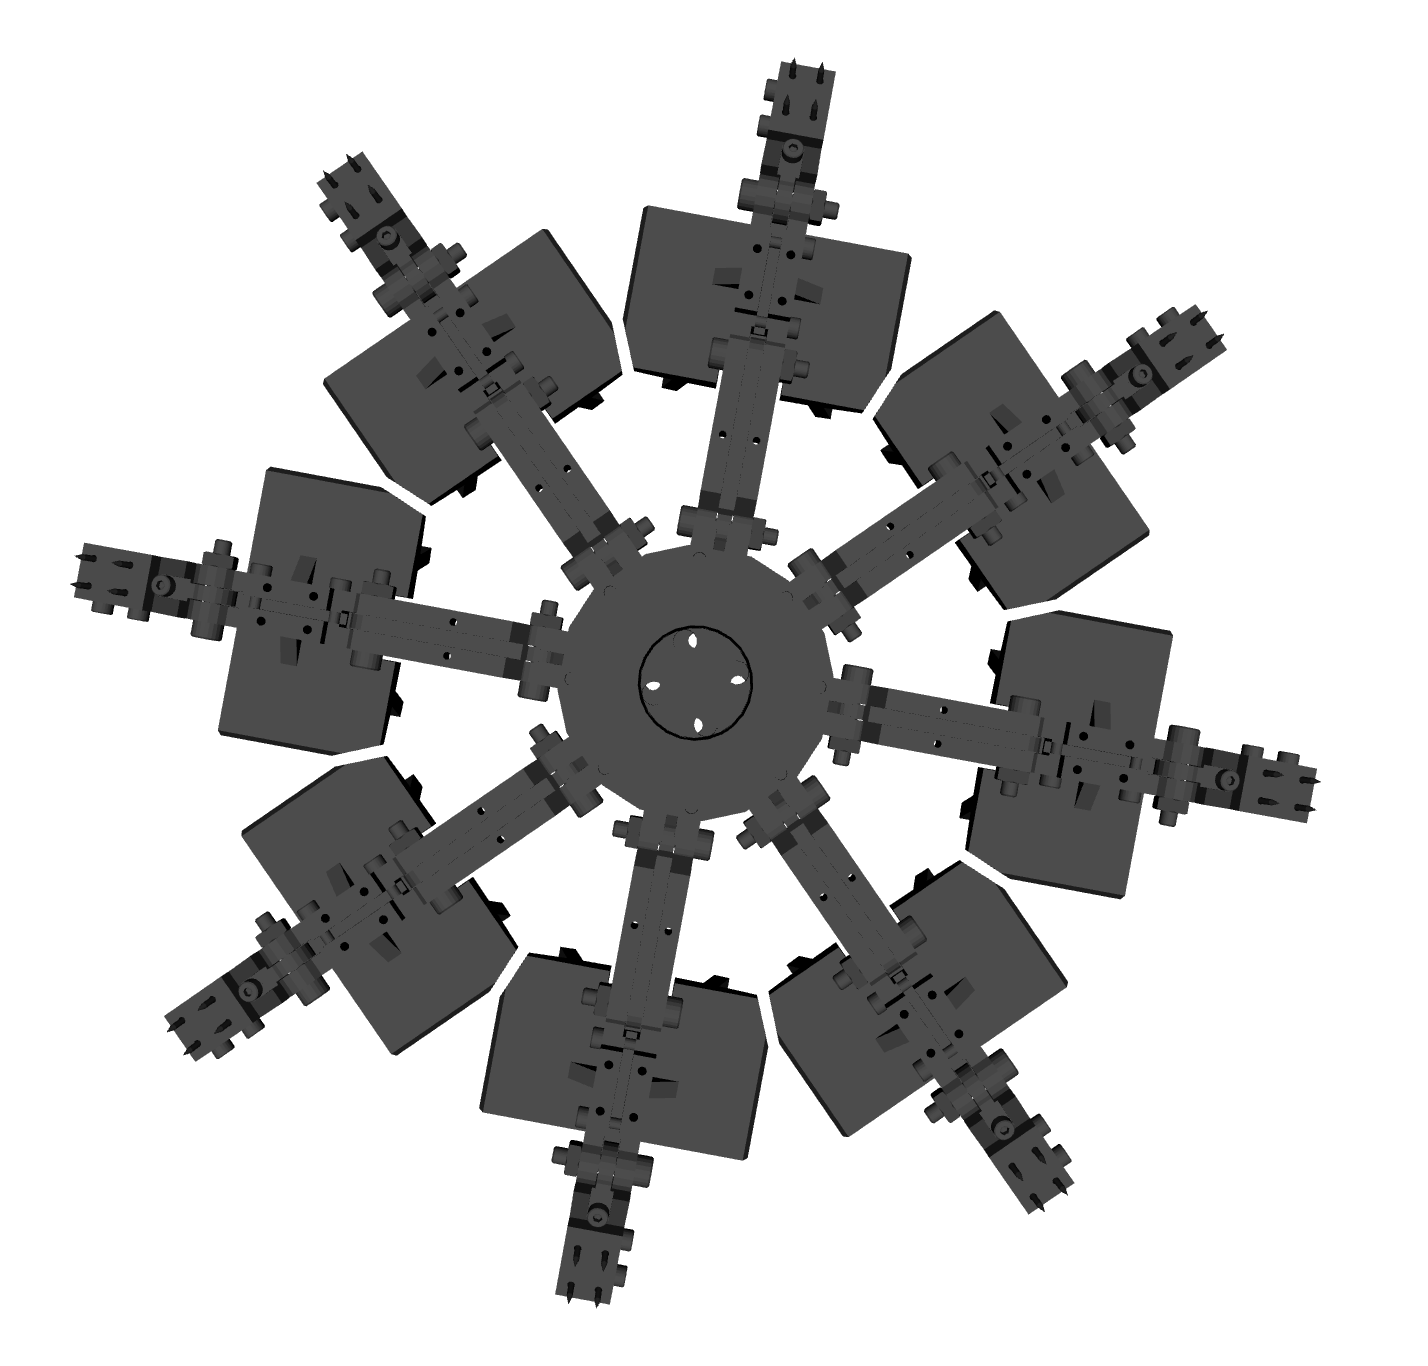
\includegraphics[width=0.90\paperwidth,
                             trim=15cm 16cm 0 0, % Set to zero or real units (e.g., 1cm 2cm 0 0)
                             clip]{G2W_0_transparent.png}
        };
    \end{tikzpicture}
    
    \clearpage
}
\newcommand{\BlankPageTLGWone}{
    \clearpage
    \thispagestyle{empty}
    \null
    
    \begin{tikzpicture}[remember picture, overlay]
        \node[anchor=south west, opacity=0.4] at (current page.south west){
            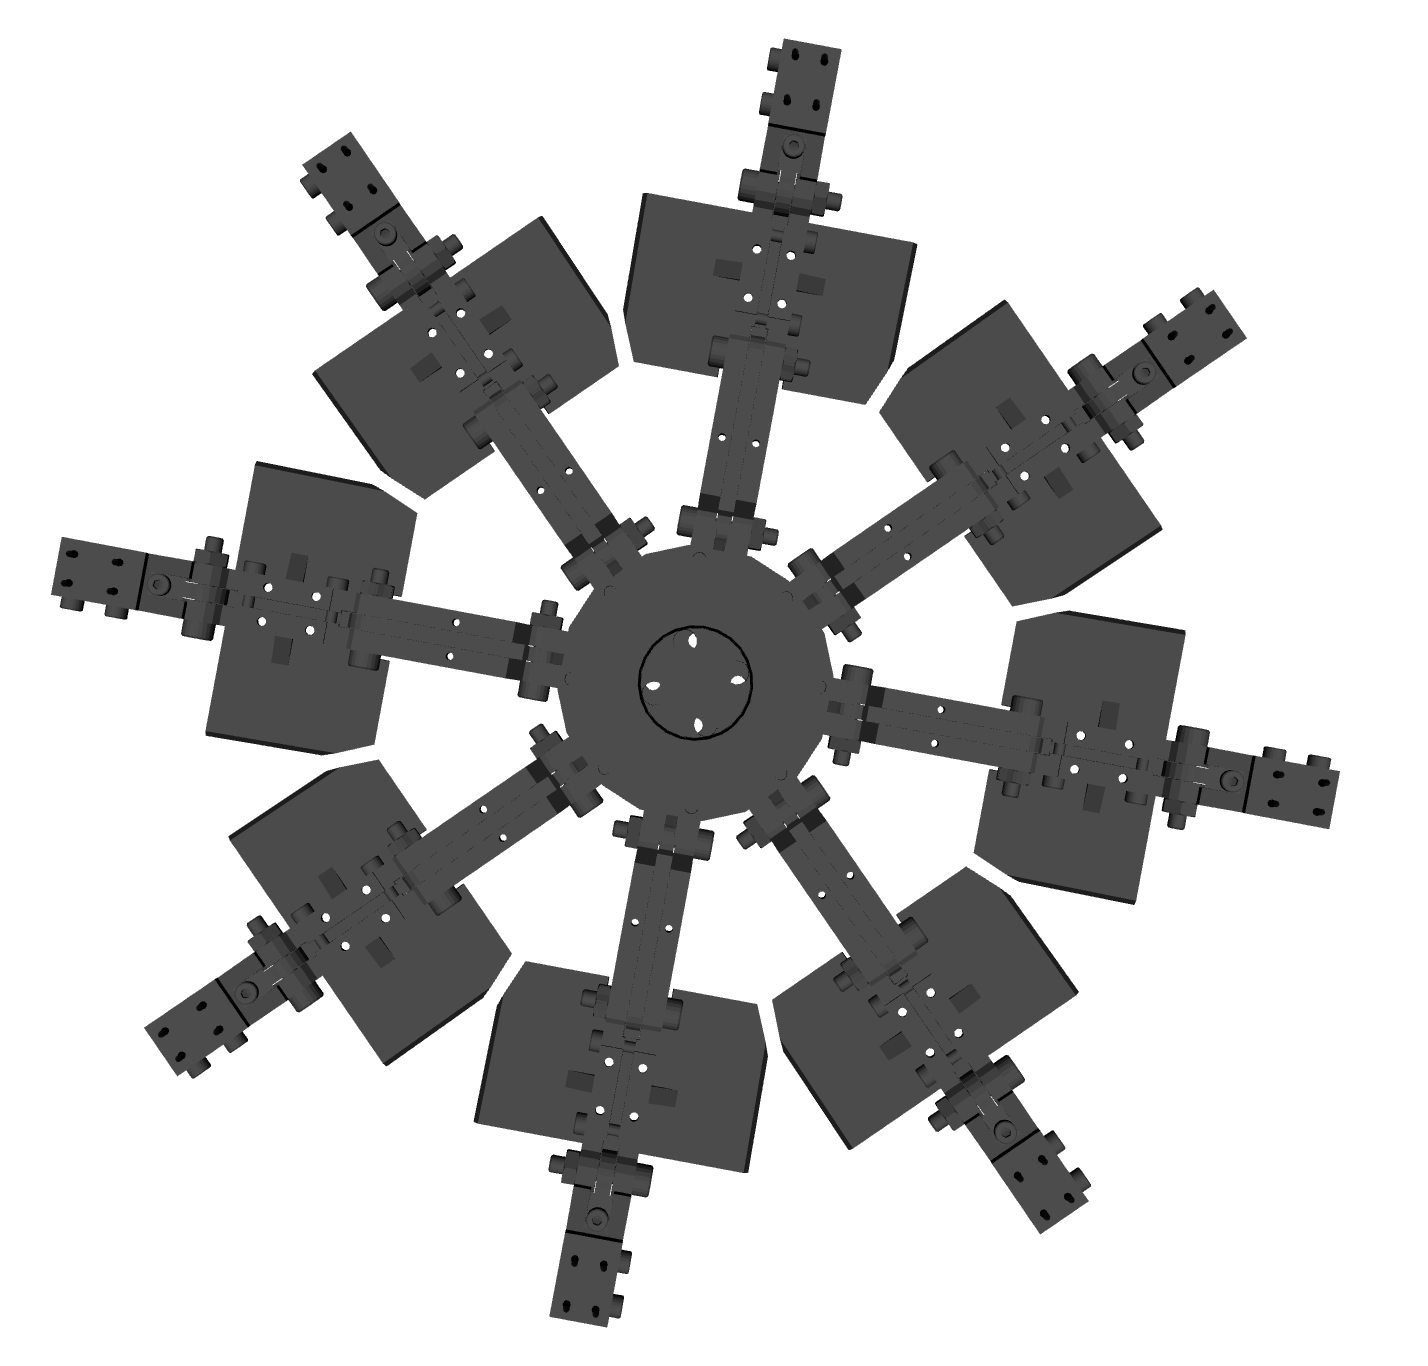
\includegraphics[width=0.90\paperwidth,
                             trim=15cm 16cm 0 0, % Set to zero or real units (e.g., 1cm 2cm 0 0)
                             clip]{G2W_1_new.png}
        };
    \end{tikzpicture}
    
    \clearpage
}
\newcommand{\BlankPageTLGWtwo}{
    \clearpage
    \thispagestyle{empty}
    \null
    
    \begin{tikzpicture}[remember picture, overlay]
        \node[anchor=south west, opacity=0.4] at (current page.south west){
            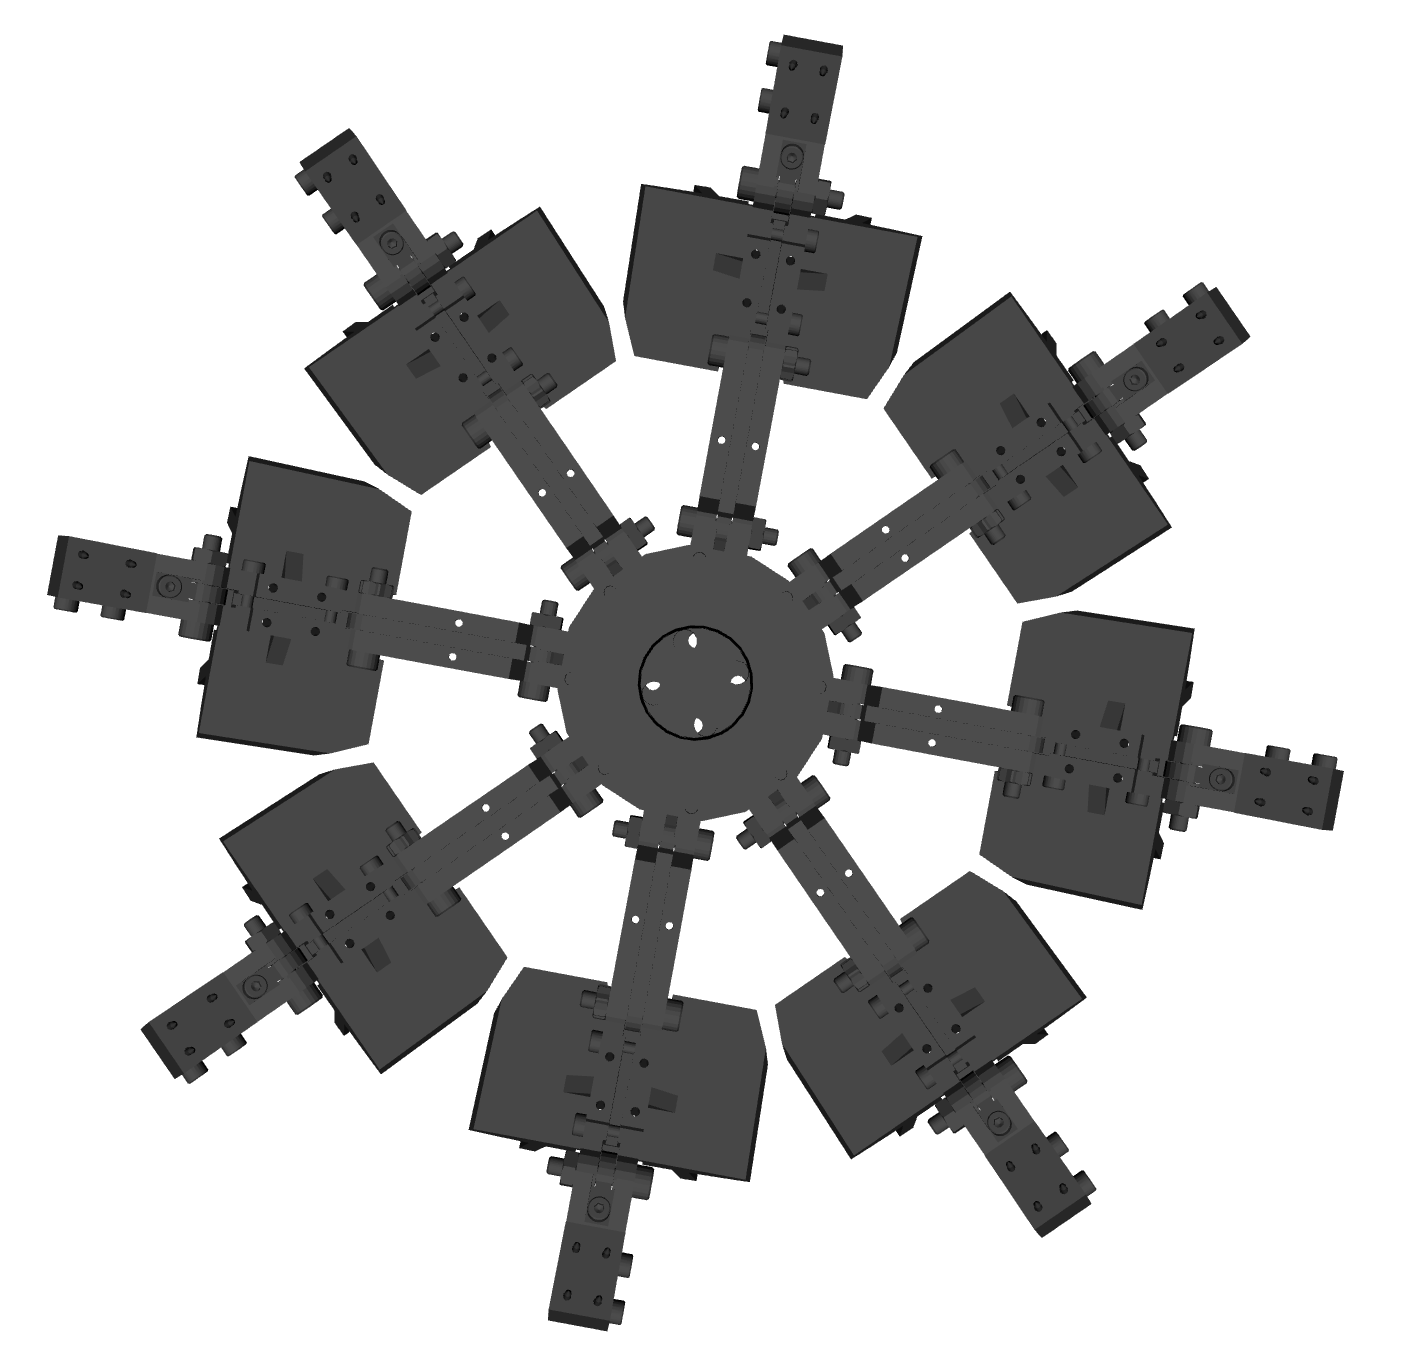
\includegraphics[width=0.90\paperwidth,
                             trim=15cm 16cm 0 0, % Set to zero or real units (e.g., 1cm 2cm 0 0)
                             clip]{G2W_2_new.png}
        };
    \end{tikzpicture}
    
    \clearpage
}
\newcommand{\BlankPageTLGWthree}{
    \clearpage
    \thispagestyle{empty}
    \null
    
    \begin{tikzpicture}[remember picture, overlay]
        \node[anchor=south west, opacity=0.4] at (current page.south west){
            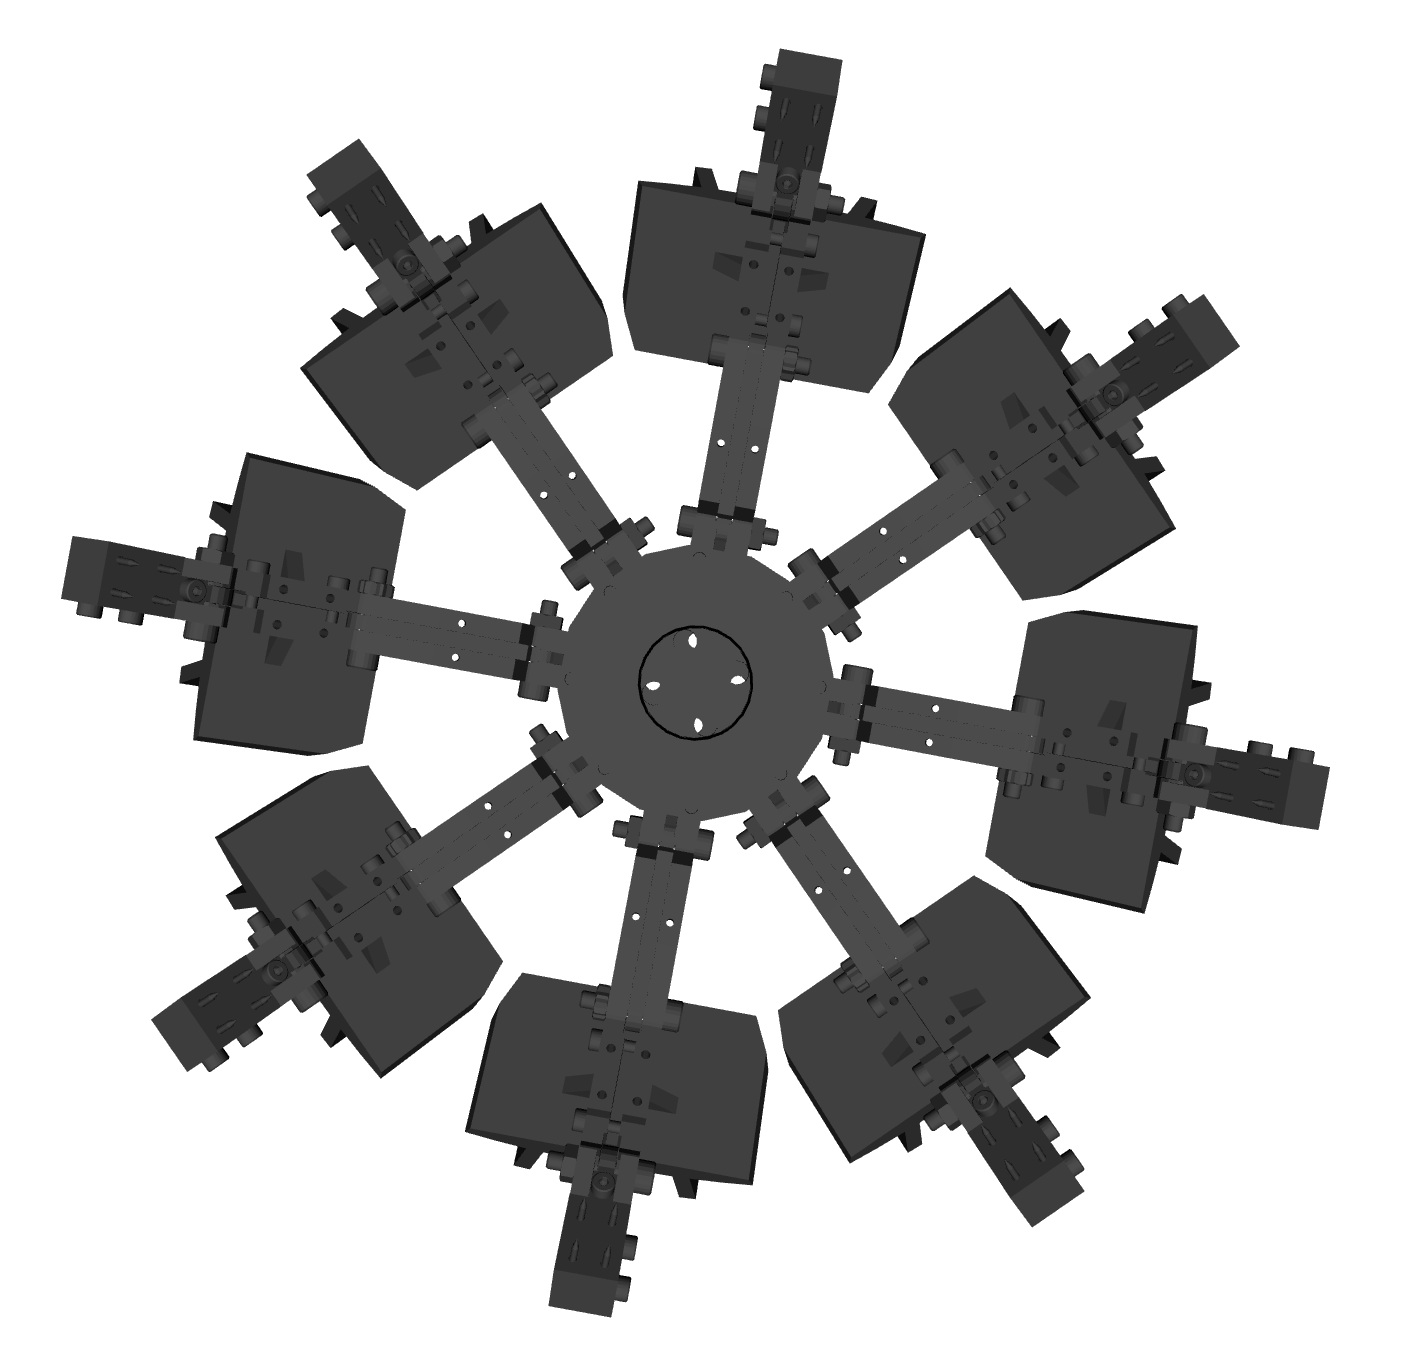
\includegraphics[width=0.90\paperwidth,
                             trim=15cm 16cm 0 0, % Set to zero or real units (e.g., 1cm 2cm 0 0)
                             clip]{G2W_3_new.png}
        };
    \end{tikzpicture}
    
    \clearpage
}
\newcommand{\BlankPageTLGWfour}{
    \clearpage
    \thispagestyle{empty}
    \null
    
    \begin{tikzpicture}[remember picture, overlay]
        \node[anchor=south west, opacity=0.4] at (current page.south west){
            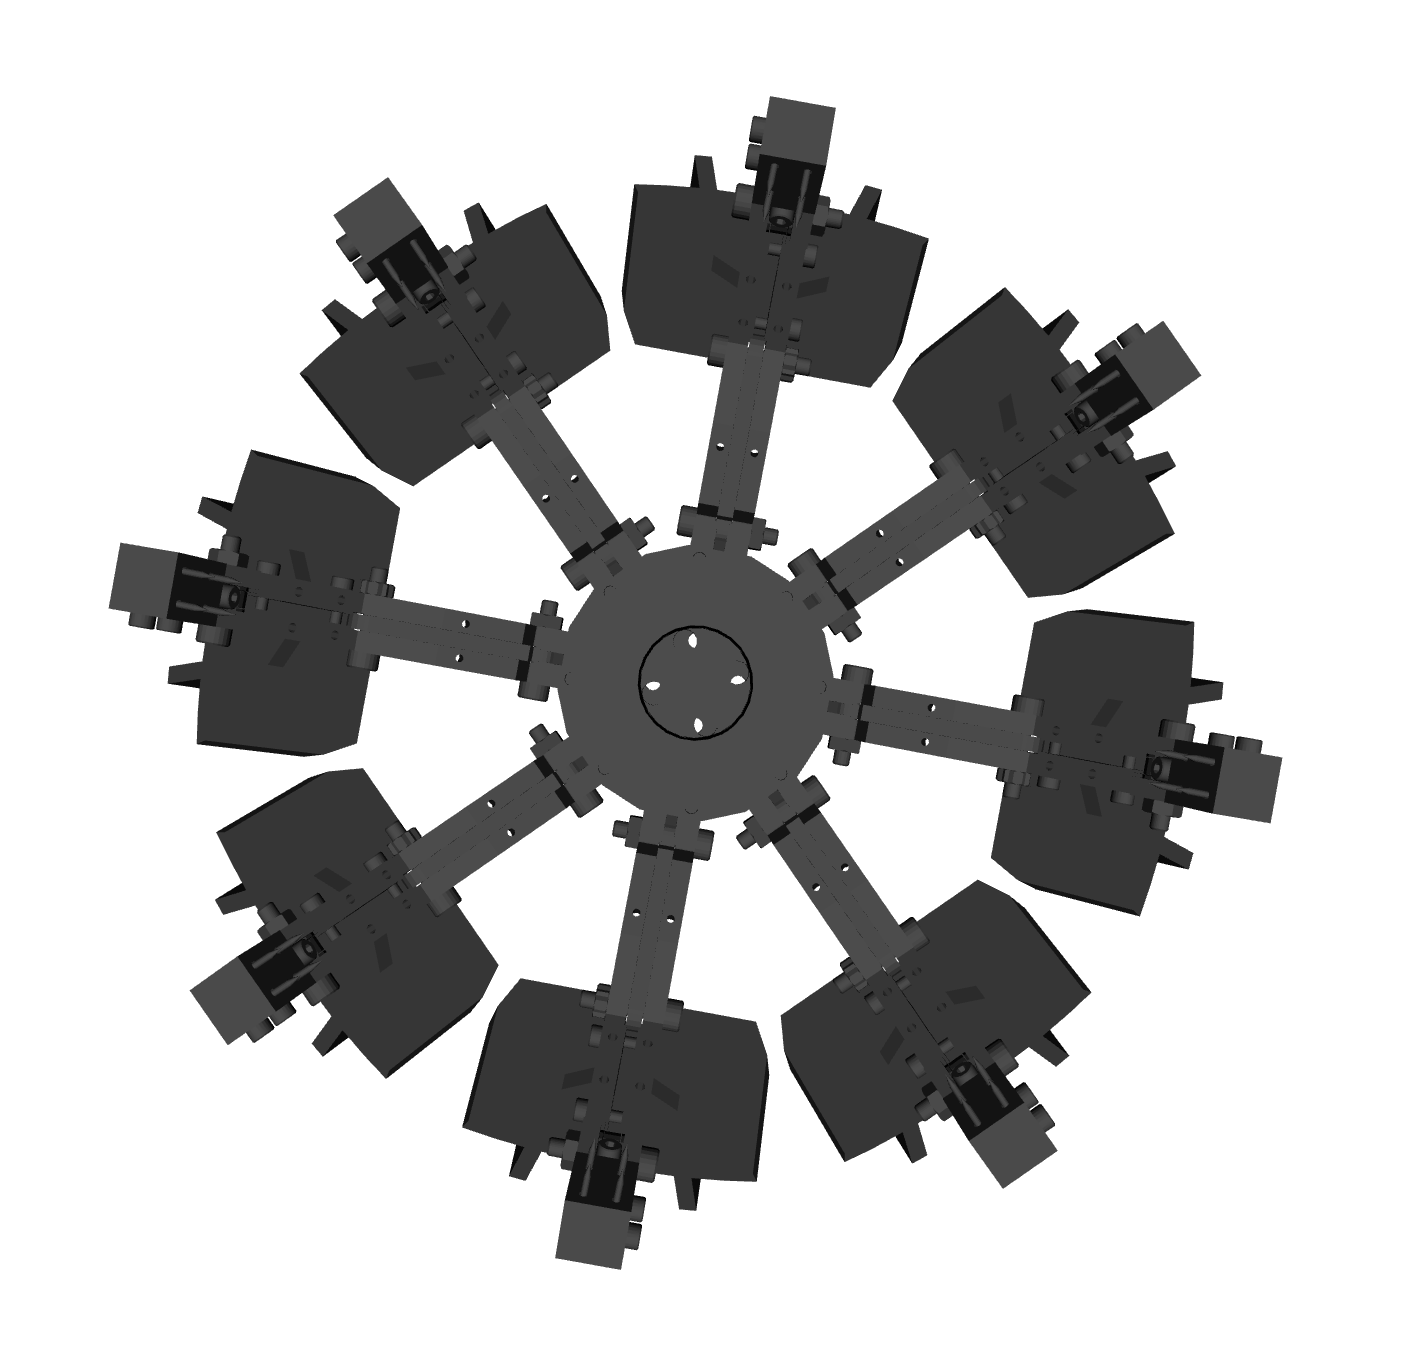
\includegraphics[width=0.90\paperwidth,
                             trim=15cm 16cm 0 0, % Set to zero or real units (e.g., 1cm 2cm 0 0)
                             clip]{G2W_4_new.png}
        };
    \end{tikzpicture}
    
    \clearpage
}
\newcommand{\BlankPageTLGWfive}{
    \clearpage
    \thispagestyle{empty}
    \null
    
    \begin{tikzpicture}[remember picture, overlay]
        \node[anchor=south west, opacity=0.4] at (current page.south west){
            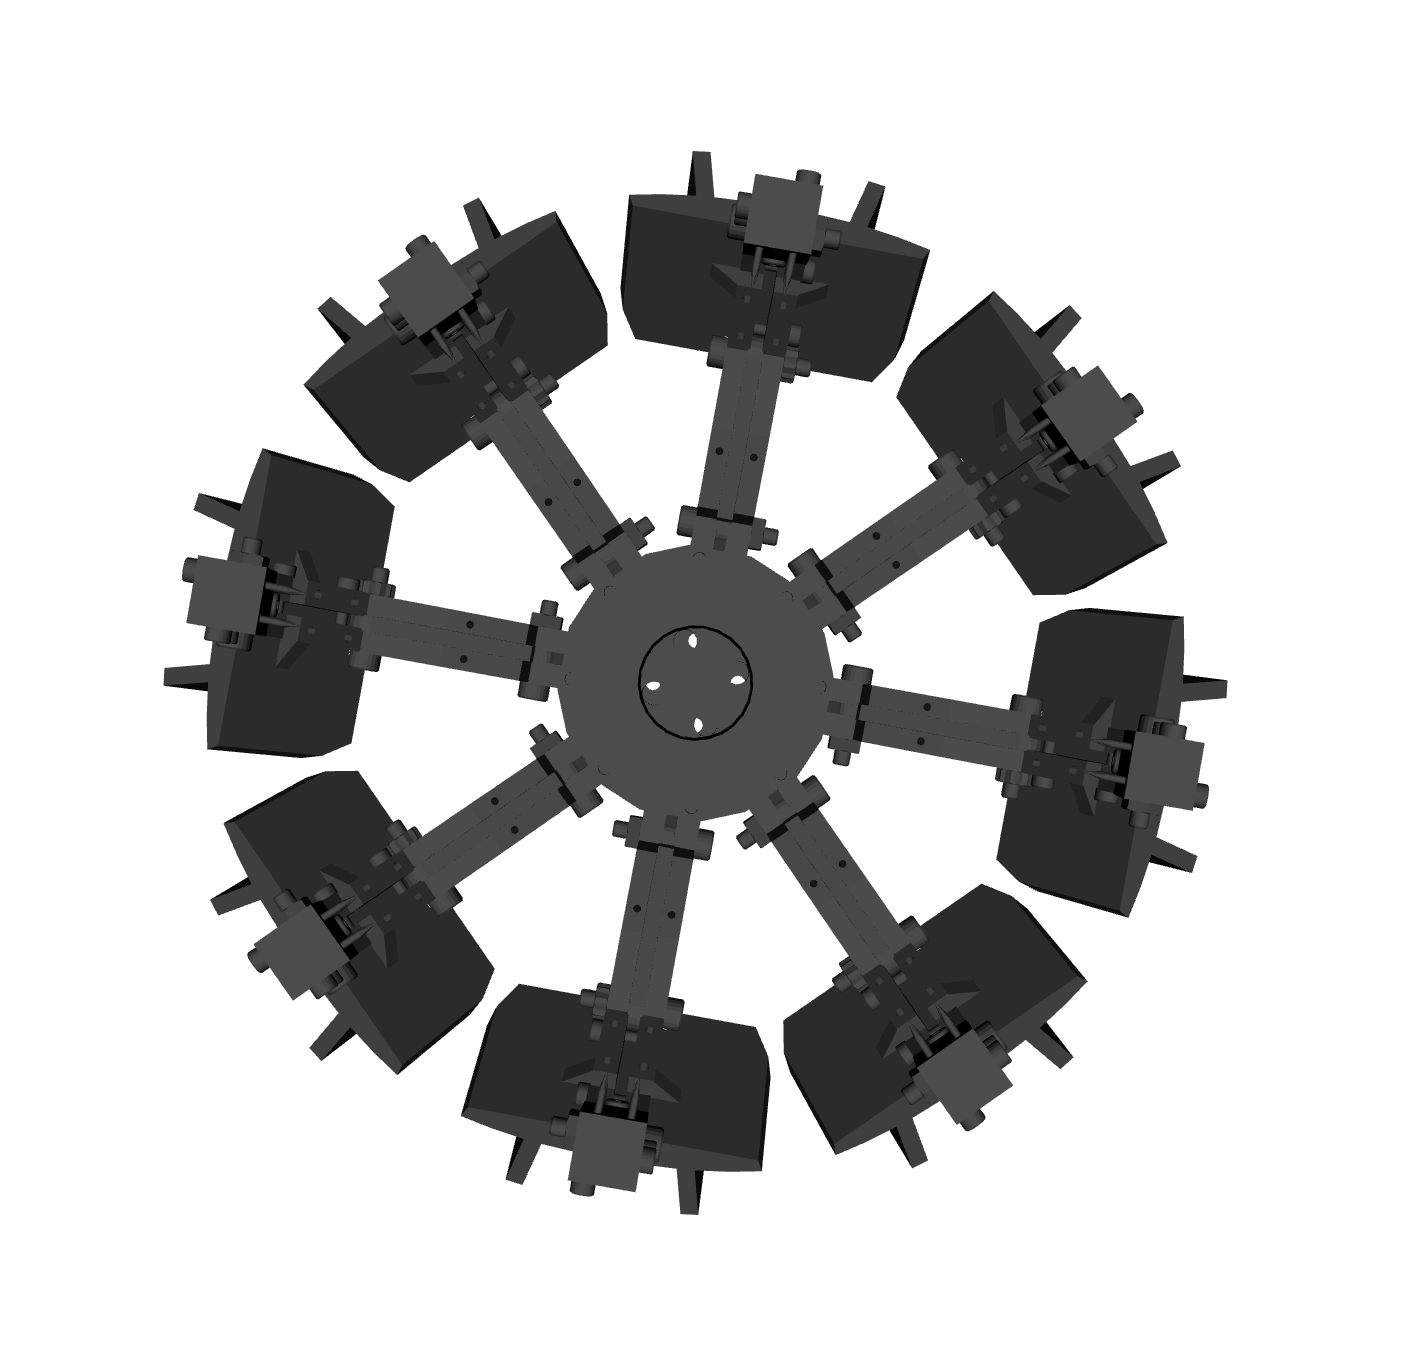
\includegraphics[width=0.90\paperwidth,
                             trim=15cm 16cm 0 0, % Set to zero or real units (e.g., 1cm 2cm 0 0)
                             clip]{G2W_5_new.png}
        };
    \end{tikzpicture}
    
    \clearpage
}
\newcommand{\BlankPageTLGWsix}{
    \clearpage
    \thispagestyle{empty}
    \null
    
    \begin{tikzpicture}[remember picture, overlay]
        \node[anchor=south west, opacity=0.4] at (current page.south west){
            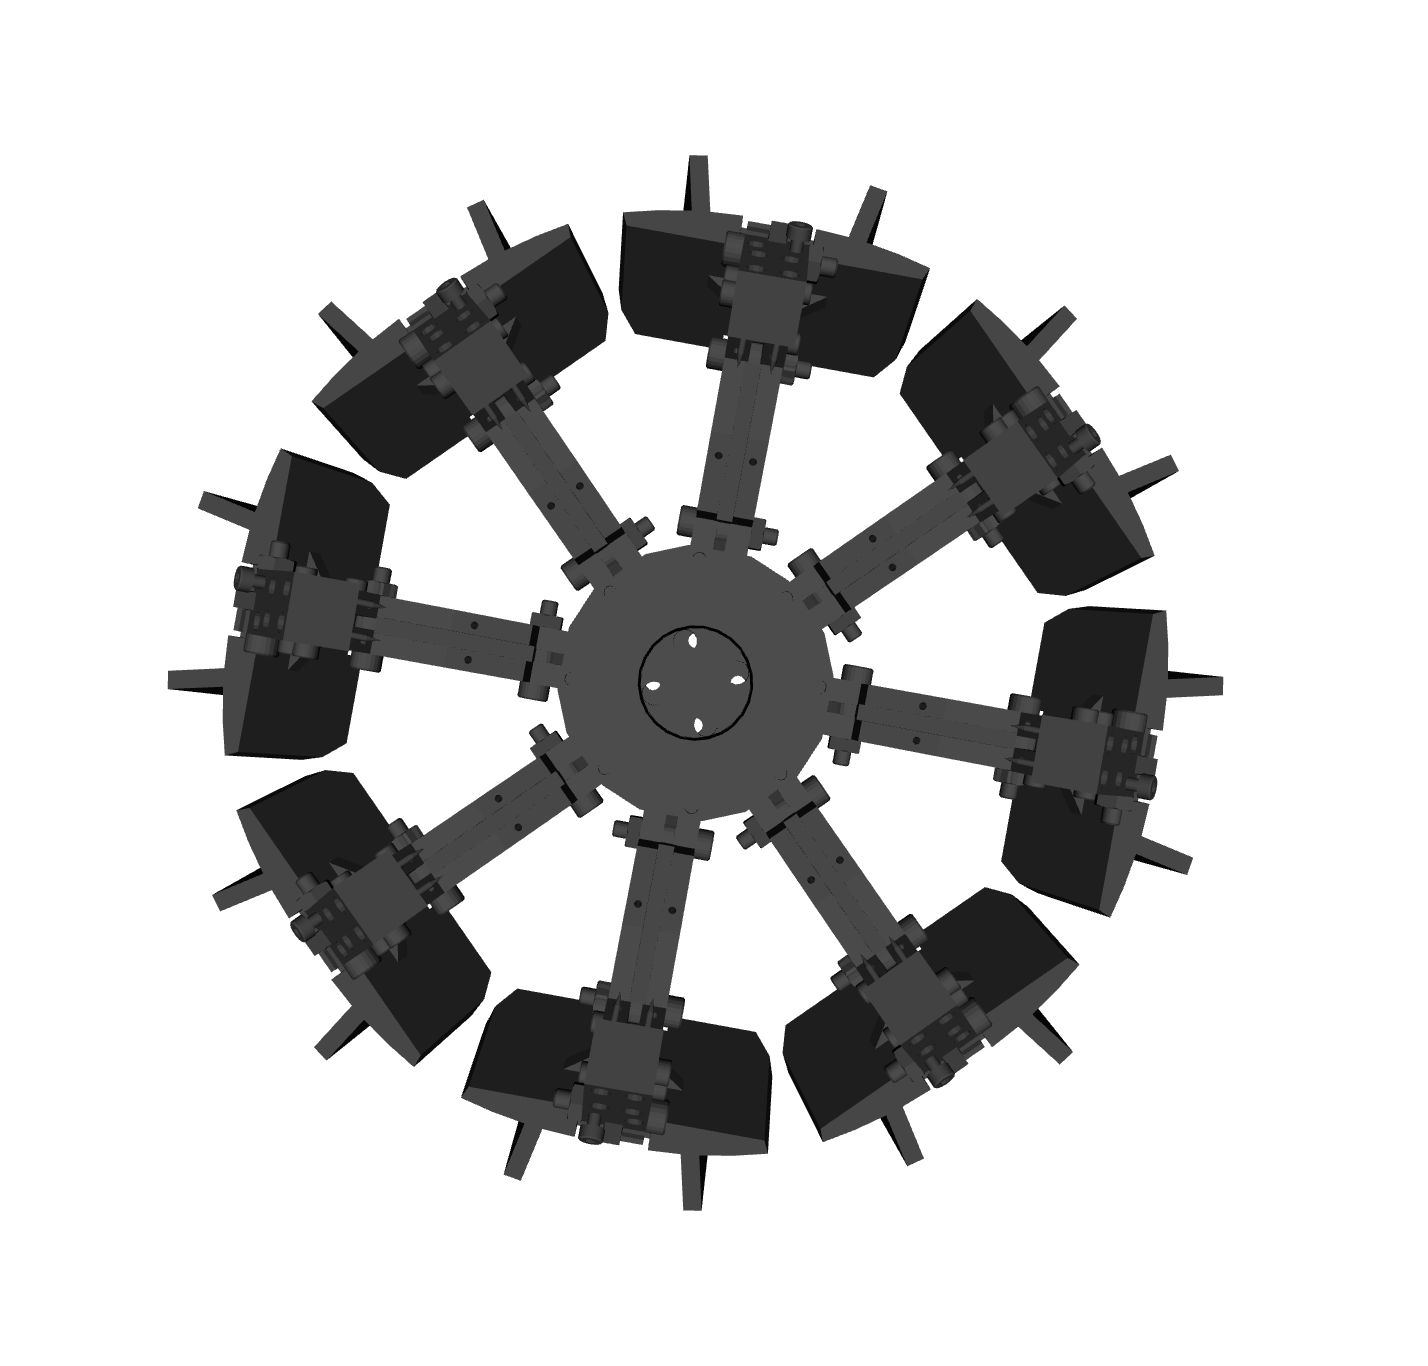
\includegraphics[width=0.90\paperwidth,
                             trim=15cm 16cm 0 0, % Set to zero or real units (e.g., 1cm 2cm 0 0)
                             clip]{G2W_6_new.png}
        };
    \end{tikzpicture}
    
    \clearpage
}
\newcommand{\BlankPageTLGWseven}{
    \clearpage
    \thispagestyle{empty}
    \null
    
    \begin{tikzpicture}[remember picture, overlay]
        \node[anchor=south west, opacity=0.4] at (current page.south west){
            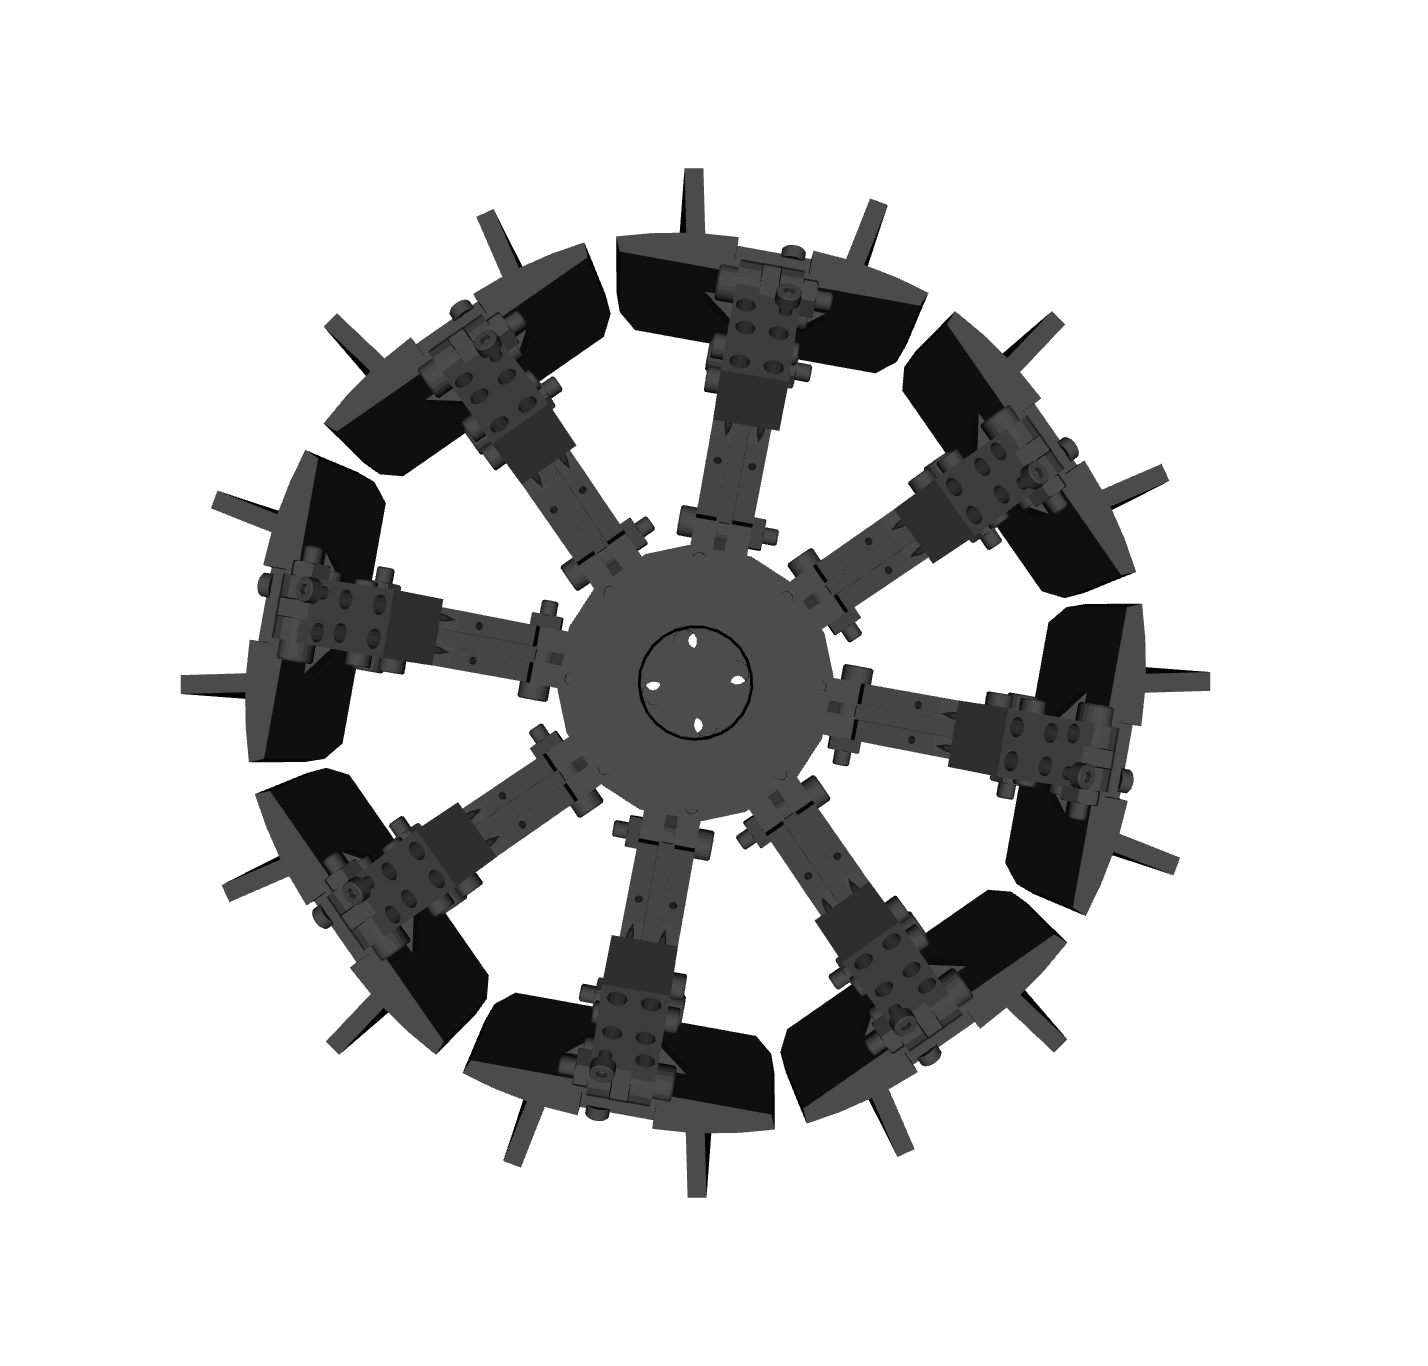
\includegraphics[width=0.90\paperwidth,
                             trim=15cm 16cm 0 0, % Set to zero or real units (e.g., 1cm 2cm 0 0)
                             clip]{G2W_7_new.png}
        };
    \end{tikzpicture}
    
    \clearpage
}
\newcommand{\BlankPageTLGWeight}{
    \clearpage
    \thispagestyle{empty}
    \null
    
    \begin{tikzpicture}[remember picture, overlay]
        \node[anchor=south west, opacity=0.4] at (current page.south west){
            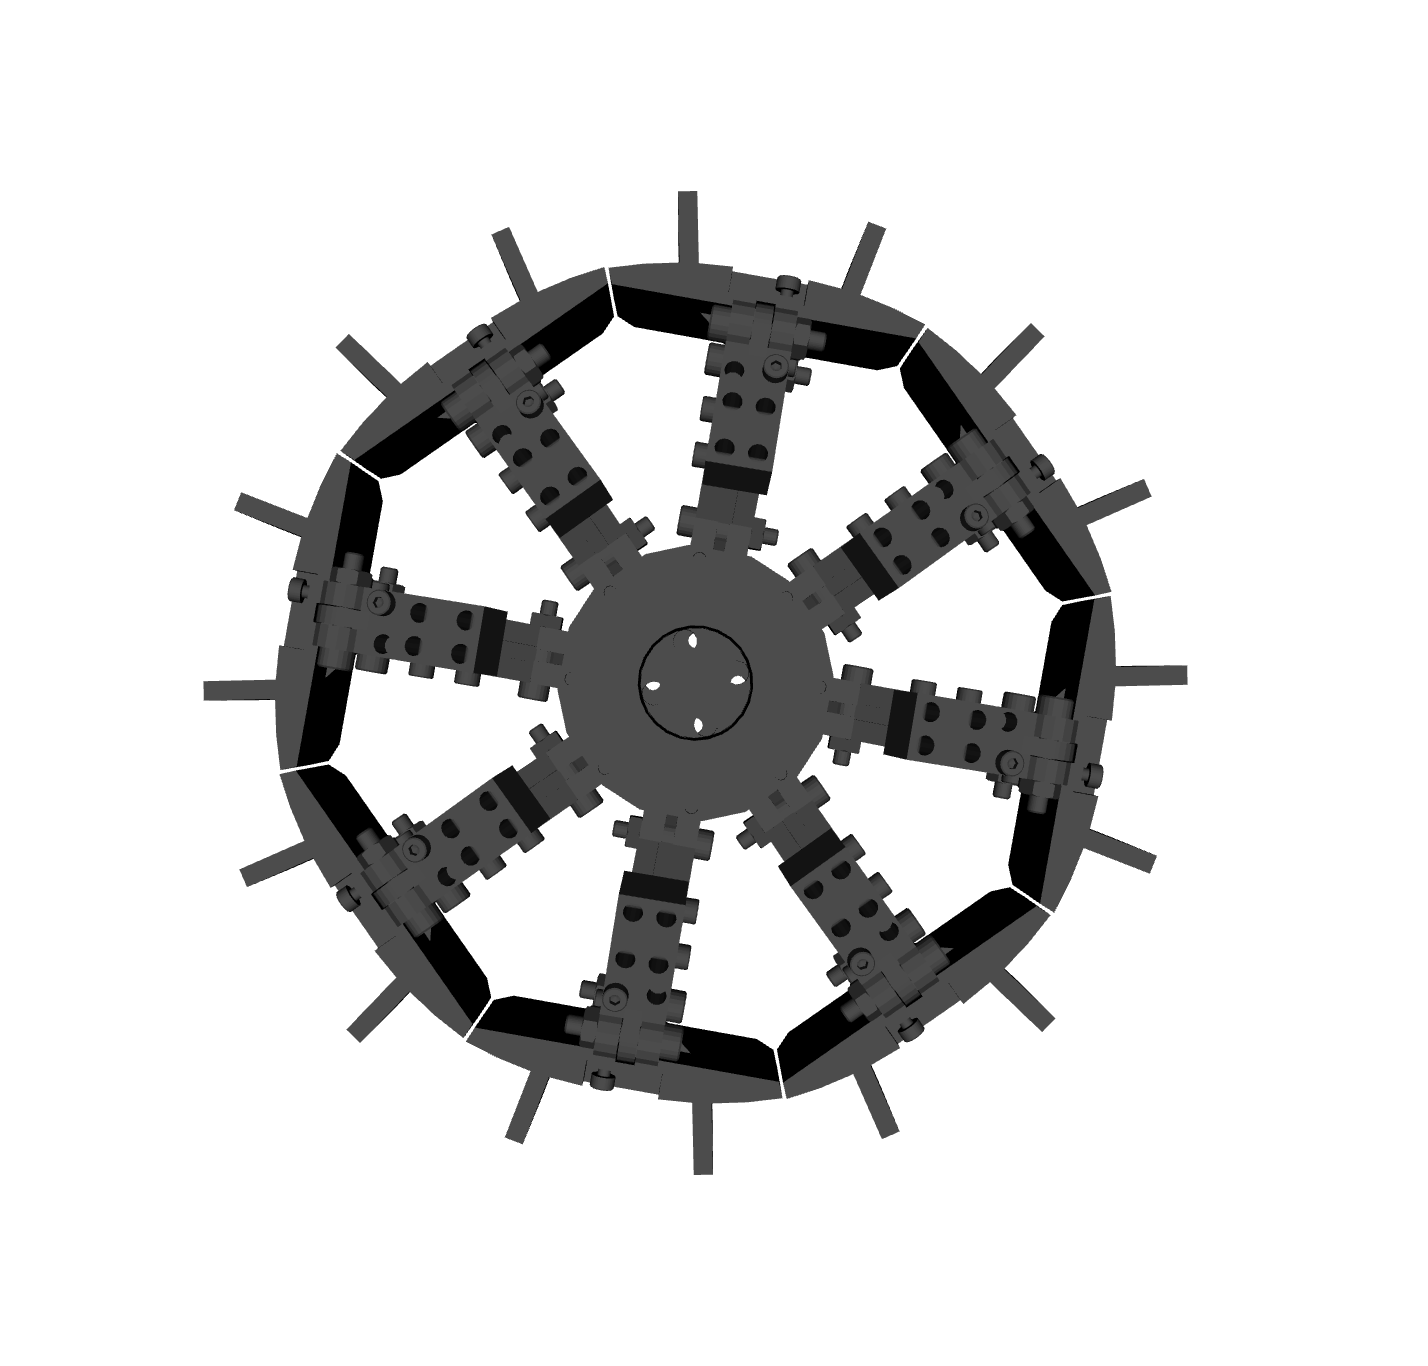
\includegraphics[width=0.90\paperwidth,
                             trim=15cm 16cm 0 0, % Set to zero or real units (e.g., 1cm 2cm 0 0)
                             clip]{G2W_8_new.png}
        };
    \end{tikzpicture}
    
    \clearpage
}
\newcommand{\BlankPageDLTRGW}{
    \clearpage
    \thispagestyle{empty}
    \null
    
    \begin{tikzpicture}[remember picture, overlay]
        \node[anchor=south west, opacity=0.4] at (current page.south west){
            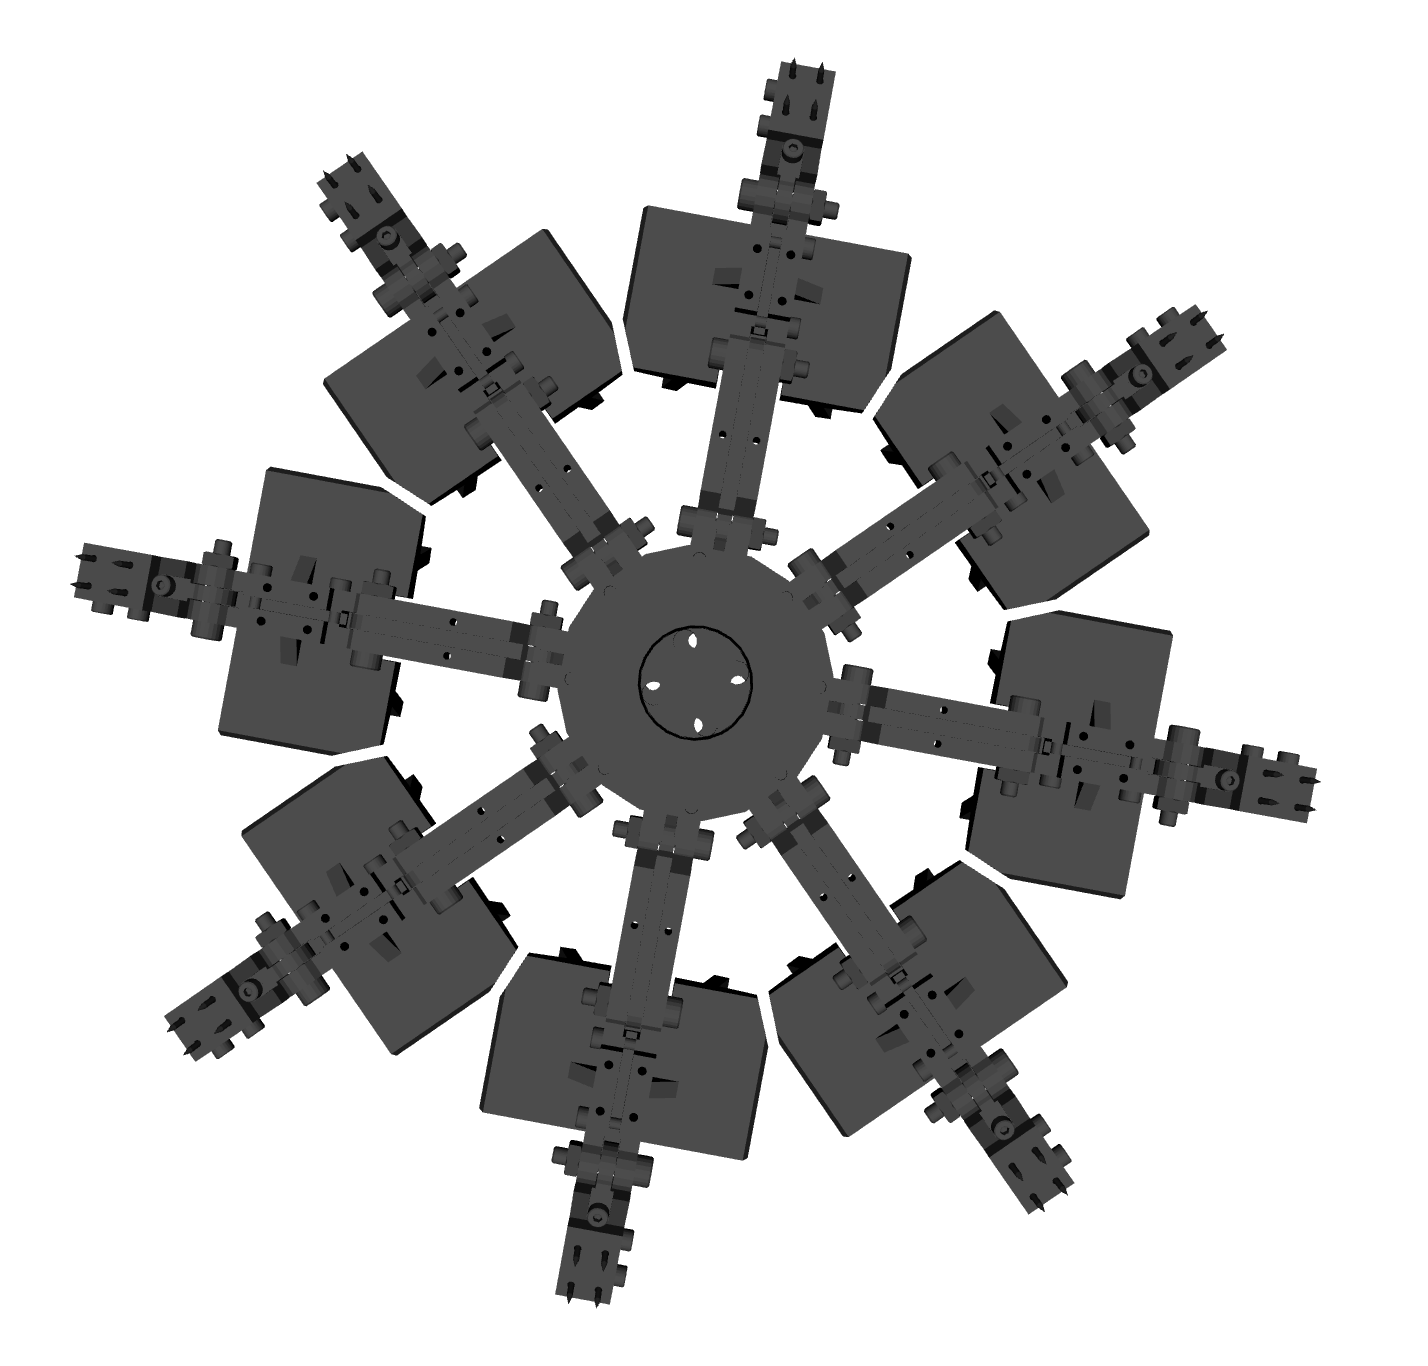
\includegraphics[width=0.80\paperwidth,
                             trim=15cm 16cm 0 0, % Set to zero or real units (e.g., 1cm 2cm 0 0)
                             clip]{G2W_0_transparent.png}
        };
    \end{tikzpicture}
    \begin{tikzpicture}[remember picture, overlay]
            \node[anchor=north east, opacity=0.4] at (current page.north east){
            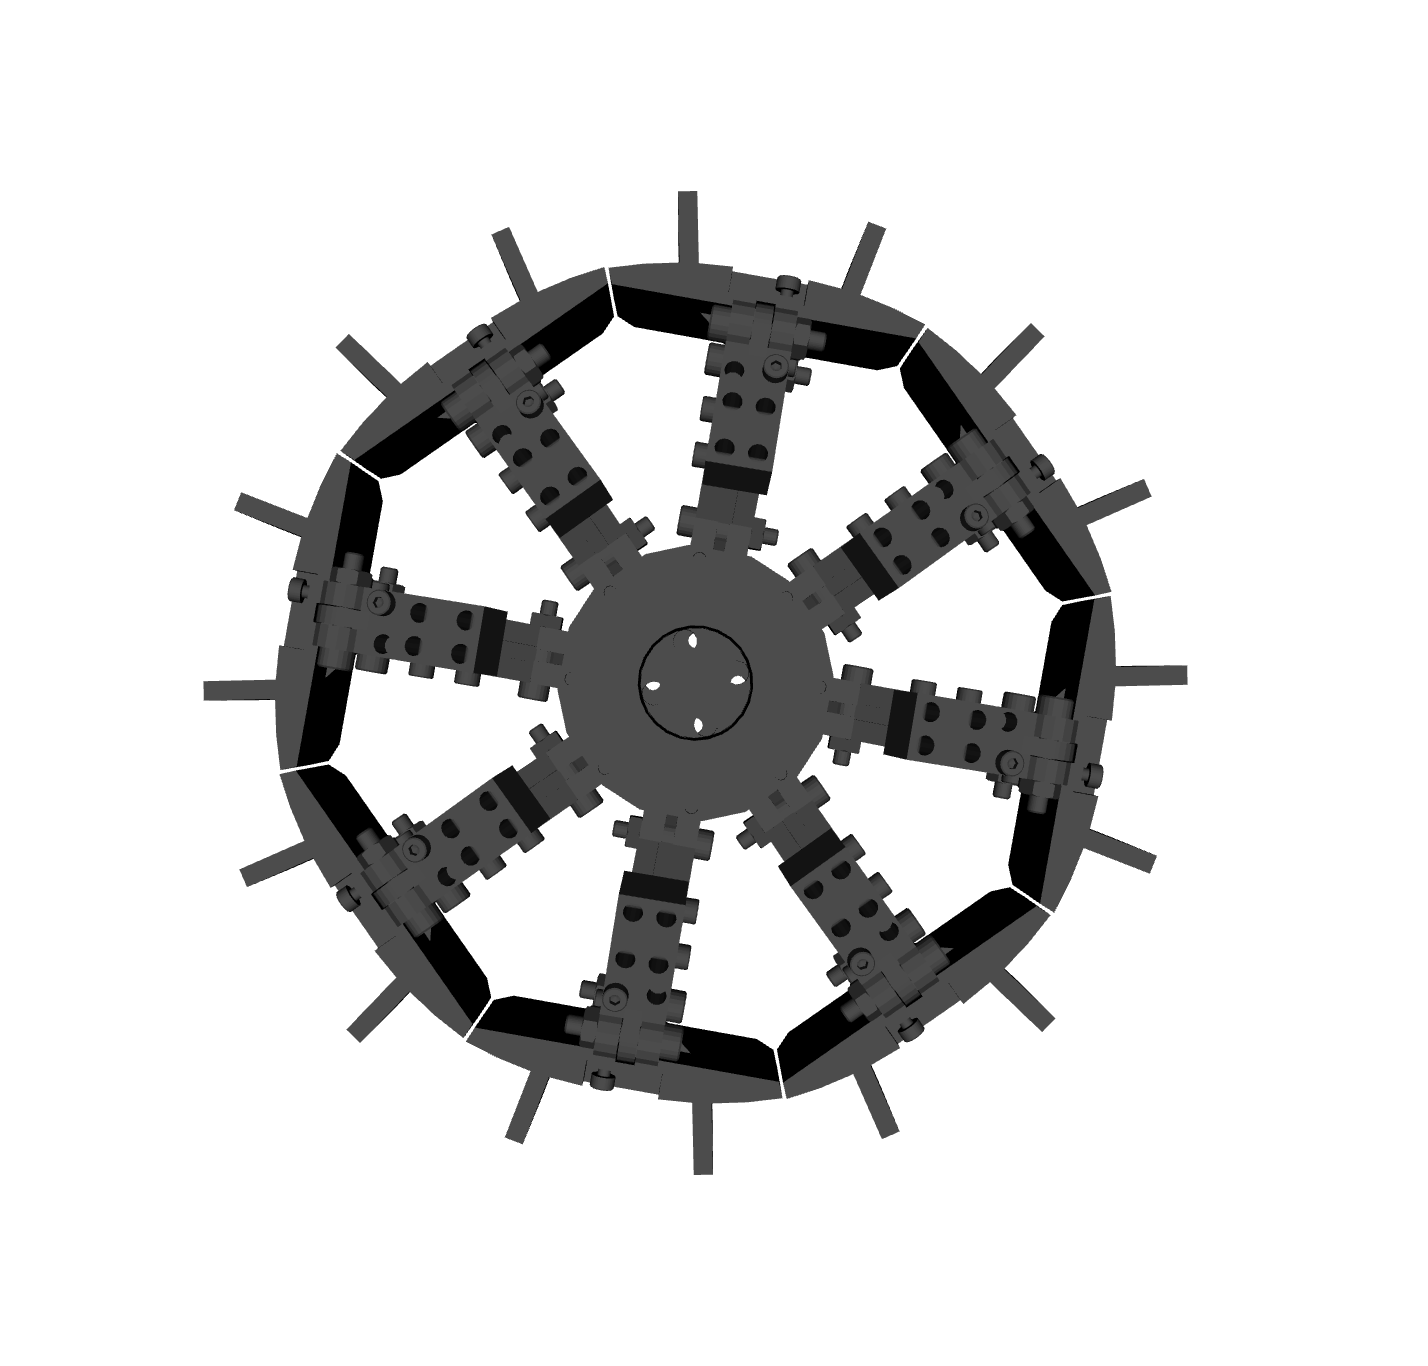
\includegraphics[width=0.80\paperwidth,
                             trim=0 0 15cm 16cm, % Set to zero or real units (e.g., 1cm 2cm 0 0)
                             clip]{G2W_8_new.png}
        };
    \end{tikzpicture}
    \clearpage
}
% EXAMPLES OF NEW COMMANDS
\newcommand{\bea}{\begin{eqnarray}} % Shortcut for equation arrays
\newcommand{\eea}{\end{eqnarray}}
\newcommand{\e}[1]{\times 10^{#1}}  % Powers of 10 notation

%----------------------------------------------------------------------------
%	BEGIN OF YOUR DOCUMENT
%----------------------------------------------------------------------------

%GLOSSARY


\usepackage[acronyms,nonumberlist]{glossaries}
\newglossarystyle{compactstyle}{
  \renewenvironment{theglossary}
    {\begin{description}%
       \setlength{\itemsep}{0pt}
     }
    {\end{description}}%
  \renewcommand*{\glossaryheader}{}%
  \renewcommand*{\glsgroupskip}{}%
}
\makeglossaries



\begin{document}

\fancypagestyle{plain}{%
\fancyhf{} % Clear all header and footer fields
\fancyhead[RO,RE]{\thepage} %RO=right odd, RE=right even
\renewcommand{\headrulewidth}{0pt}
\renewcommand{\footrulewidth}{0pt}}

%----------------------------------------------------------------------------
%	TITLE PAGE
%----------------------------------------------------------------------------

\pagestyle{empty} % No page numbers
\frontmatter % Use roman page numbering style (i, ii, iii, iv...) for the preamble pages

\puttitle{
	title={Motion Control and Manipulability Analysis of LIMBERO-GRIEEL: \\ a Multimodal Limbed Robot for Unstructured Environments}, % Title of the thesis
	name={Alessandro Puglisi}, % Author Name and Surname
	course={Automation and Control Engineering}, % Study Programme (in Italian)
	ID  = {221465},  % Student ID number (numero di matricola)
	advisor= {Prof. Luca Bascetta}, % Supervisor name
	coadvisor={Prof. Kazuya Yoshida}, % Co-Supervisor name, remove this line if there is none
	academicyear={2024-25},  % Academic Year
} % These info will be put into your Title page 

%----------------------------------------------------------------------------
%	PREAMBLE PAGES: ABSTRACT (inglese e italiano), EXECUTIVE SUMMARY
%----------------------------------------------------------------------------
\clearpage
\thispagestyle{empty} % This removes the header/footer but keeps the numbering
\vspace*{\fill} % Pushes everything to the bottom
\newpage

% ABSTRACT IN ENGLISH
\chapter*{Abstract} 

Crucial scientific and social activities such as environmental monitoring, exploration of extreme environments, and disaster response have relied on teleoperated robotic systems for as long as these technologies have existed.
Those operations are conducted in dangerous or unreachable environments for humans, where the deployment of machines capable of achieving multiple tasks is inevitable. A clear example is planetary exploration, conducted mainly with wheeled mobile robots since the first remotely operated rover landed on the lunar surface in 1970. 

In recent years, achievements such as improved computing capabilities, 3D perception, environmental awareness, and advanced control techniques have made autonomous systems possible. Furthermore, novel mechanical designs and actuation systems enable locomotion in terrains where moving on wheels is unfeasible. Walking, climbing, flying, and swimming robots are conquering unstructured environments.
However, to complete complex tasks in those settings, a unique locomotion mode is not enough, and the development of multimodal robotic systems is an active research nowadays.     


The robotic system considered in this research is a multimodal four-limbed machine, with walking, climbing, and driving capabilities, thanks to the employed gripper-wheel transformable end effector. This system's multiple locomotion modes and manipulation abilities enable the efficient execution of complex missions, otherwise requiring the simultaneous deployment of different conventional robots.

This cutting-edge machine is currently a prototype of the Space Robotics Lab, and this work contributes to its first development steps, with the design and implementation of reliable high-level motion algorithms, motion controller design, software architecture integration, simulation setup, and first real system experiments. 

The principal algorithm developed enables a smooth autonomous and adaptable module transformation, maintaining the robot stable with three limbs on the ground while transforming the raised limb. In computing the motion sequence, anticipative planning is used, and feedback from the system state adapts the tasks, considering dexterity and stability in defining the next robot configuration. 

The literature lacks an index of dexterity for multilimbed robots, for this reason, in this research a novel criterion has been defined, extending the theory on robotic arm manipulability ellipsoid. This index proves to be efficient in defining the preferred direction of motion of the robot base in a given configuration. Furthermore, this performance criterion has been tested in the bio-inspired example of a jumping grasshopper. 

The algorithm and the motion controller have been developed and tested into a simulator, configured as part of this research. Finally, tests on the real system have been conducted.

This work has defined the foundation of smooth locomotion transition and system autonomy, still under research for a novel mechanical design. In addition, many future design requirements and components have been derived from the system analysis. 



\vspace{0.5em}
\noindent\textbf{Keywords:} field robotics, multimodal robotics, motion control,manipulability analysis, ROS2, simulation.% Keywords


% ABSTRACT IN ITALIAN
\chapter*{Abstract in lingua italiana}
Attività scientifiche e sociali di fondamentale importanza, quali il monitoraggio ambientale, l’esplorazione di ambienti estremi e la risposta a situazioni di emergenza, si sono da sempre affidate a sistemi robotici operati da remoto. Tali operazioni vengono condotte in ambienti pericolosi o inaccessibili per l’essere umano, dove il dispiegamento di macchine in grado di svolgere molteplici compiti risulta inevitabile. Un chiaro esempio è rappresentato dall’esplorazione planetaria, realizzata principalmente mediante robot mobili su ruote sin dal primo rover teleoperato atterrato sulla superficie lunare nel 1970.

Negli ultimi anni, progressi significativi nelle capacità computazionali, nella percezione 3D, nella consapevolezza ambientale e nelle tecniche di controllo avanzato hanno reso possibile lo sviluppo di sistemi autonomi. Inoltre, innovativi design meccanici e sistemi di attuazione consentono oggi la locomozione in terreni dove muoversi su ruote risulta impraticabile. Sistemi robotici in grado di camminare su gambe, arrampicarsi, volare e nuotare stanno conquistando ambienti non strutturati. Tuttavia, per completare compiti complessi in tali contesti, una modalità di locomozione unica non è sufficiente, e lo sviluppo di sistemi robotici multimodali rappresenta oggi un campo di ricerca attivo.

Il sistema robotico considerato in questa ricerca è una macchina multimodale a quattro arti, dotata di capacità di camminare, arrampicarsi e muoversi su ruote, grazie all’end-effector impiegato, trasformabile da ruota a gripper e viceversa. Le molteplici modalità di locomozione e le capacità manipolative di questo sistema permettono l’esecuzione efficiente di missioni complesse che, altrimenti, richiederebbero il dispiegamento simultaneo di differenti robot convenzionali.

Questa macchina all’avanguardia è attualmente un prototipo sviluppato dallo Space Robotics Lab (Tohoku Univeristy, JP), e il presente lavoro contribuisce ai suoi primi passi di sviluppo, con la progettazione e l’implementazione di algoritmi di pianificazione del moto ad alto livello, il design del controller del moto, l’integrazione dell’architettura software, la configurazione dell’ambiente di simulazione e i primi esperimenti sul sistema reale.

L’algoritmo principale sviluppato consente una trasformazione autonoma, fluida e adattabile del end-effector. La stabilità del robot è garantita da tre arti a contatto con il suolo, durante il quale l’arto sollevato viene trasformato. 
Nella computazione della sequenza di movimento viene impiegata una pianificazione anticipativa, e il feedback dallo stato del sistema consente l’adattamento dei task, considerando destrezza e stabilità nella definizione della successiva configurazione del robot.

La letteratura attuale risulta priva di un indice di destrezza per robot multi-limbed, e in questa ricerca è stato definito un nuovo criterio per la sua valutazione, come estensione dell’ellissoide di manipolabilità dei bracci robotici. Questo indice si dimostra efficace nell’identificare la direzione ottimale di movimento della base del robot in una data configurazione degli arti. Inoltre, tale criterio di performance è stato testato sull’esempio bio-ispirato di un grillo in fase di salto.

L’algoritmo e il controller del moto sono stati sviluppati e testati in un simulatore, configurato durante questa ricerca. Infine, sono state condotte prove sul sistema reale.

Questo lavoro ha definito le basi per una transizione fluida tra diverse modalità di locomozione e per l’autonomia del sistema, aspetti tuttora in fase di studio in relazione al nuovo design meccanico. Inoltre, dall’analisi del sistema sono stati derivati numerosi requisiti e componenti per i futuri sviluppi progettuali.


\vspace{0.5em}
\noindent\textbf{Parole chiave:} robotica in ambienti non strutturati, robotica multimodale, controllo del movimento, analisi di manipolabilità, ROS2, simulazione.% Keywords (italian)

% ACKNOWLEDGEMENTS
\chapter*{Acknowledgements}

The story of this thesis begins a year ago, in March 2024, landing in Kyoto during the Sakura season (cherry blossom). The blooming of my research has lasted for a year since that time, and it has been the period of my academic studies in which I started to love what I do. I want to thank Professor Yoshida Kazuya that accept me as a research student at the Space Robotics Lab, giving me the possibility to work on something unique in the world. I would like to thank my advisor, Professor Luca Bascetta, for his support in critical moments of this research.
My work in Japan would not be possible without the help of Associate Professors Shreya Santra and Kentaro Uno, their continuous feedback and their kind words of appreciation gave me the motivation to keep going. I also want to thank the members of the SRL who support my vision there, especially Takada and Naoki, who helped me during my stay and continue to exchange ideas. I would love to work together again, pushing the boundaries of robotics research in exploring the unknown. 

Adesso i ringraziamenti entrano nella fase emotiva...Voglio dedicare questa tesi a mia nonna Renate, che mi ha trasmesso la sua determinazione e un filtro da artista sul mondo. Ai miei genitori (mamma, papà e zia Luisa – sì, io ne ho tre), che sono un faro per me e mi hanno insegnato che, ogni tanto, dei sacrifici sono necessari (come mi ha dimostrato questa tesi), ma che le soddisfazioni eclissano ogni fatica. La pazzia e l’ostinatezza di mio padre, la precisione di mia zia, la curiosità e l’instancabilità di mia madre sono state fondamentali, e mi accompagneranno sempre. 

Cecilia mi ha permesso di fare una seconda laurea in medicina, vivendo tutte le ansie di un esame di semeiotica o eziopatologia. Lei è stata la mia più grande fan, come io sono il suo, e ha reso Milano una bella città in cui ritornare dopo ogni festività passata giù. Grazie a lei questi anni sono stati pieni di colori, sorrisi, ed esperienze, anche quando il cielo era grigio. Questo primo passo verso una nuova fase della mia vita lo dedico anche a te. 

La cuginanza e gli zii andrebbero ringraziati uno ad uno: mi hanno fatto sentire a casa. Tra pranzi domenicali in famiglia, birrette,e serate in bici vagando per milano, senza di loro questi cinque anni non sarebbero stati gli stessi. Ovviamente va ringraziata anche la rimanente parte della cuginanza e i miei amici in Sicilia, per avermi dato un motivo per sopravvivere fino all’estate ogni anno.
Trasferirsi a Milano mi ha avvicinato di più alla parte della famiglia "emigrata", riducendo finalmente la distanza fisica che ci ha sempre separato. Grazie Bea, che mi hai reso una persona più critica, incazz**** verso le inguistizie e con un occhio sempre attento a ciò che mi succede attorno. Grazie a los Santos e Iago, fratelli e compagni di vita, tra pazzia, nosense ed esperienze indimenticabili. Cami e Ludo, tra iperattività e "ciaeee", Sere, Giuli, Iaffio e Vivi, grazie a tutti. Grazie anche ad un Siculo-Arabo-Ispanico, e tutti i miei amici che da ormai più di 5 anni aspettano ogni mio ritorno a casa.  

Le persone incontrate durante questi anni al Politecnico che ho ancora accanto sono ormai una parte integrante della mia vita, e non intendo chiudere questi rapporti con le conclusioni di questa tesi.
Pazzi di biorobot, fanatici di treni, gymbro, gattini dell'Agorà, amanti delle matrici, e chi più ne ha più ne metta, tutto questo non sarebbe stato lo stesso senza di voi. 

Se tu, lettore, stai per leggere questa tesi, ti auguro buona fortuna e ti ringrazio. Questo lavoro è stato una soddisfazione, seguito da mille problemi, e poi di nuovo soddisfazioni. Sono fiero dei risultati ottenuti e spero che il lavoro svolto possa ispirarti, come ha fatto con me.



%----------------------------------------------------------------------------
%	LIST OF CONTENTS/FIGURES/TABLES/SYMBOLS
%----------------------------------------------------------------------------

% TABLE OF CONTENTS
\thispagestyle{empty}
\tableofcontents % Table of contents 
\thispagestyle{empty}
\cleardoublepage

%-------------------------------------------------------------------------
%	THESIS MAIN TEXT
%-------------------------------------------------------------------------
% In the main text of your thesis you can write the chapters in two different ways:
%
%(1) As presented in this template you can write:
%    \chapter{Title of the chapter}
%    *body of the chapter*
%
%(2) You can write your chapter in a separated .tex file and then include it in the main file with the following command:
%    \chapter{Title of the chapter}
%    \input{chapter_file.tex}
%
% Especially for long thesis, we recommend you the second option.

\addtocontents{toc}{\vspace{2em}} % Add a gap in the Contents, for aesthetics


% --------------------------------------------------------------------------
% NUMBERED CHAPTERS % Regular chapters following
% --------------------------------------------------------------------------
% LIST OF SYMBOLS
% Write out the List of Symbols in this page
\chapter*{List of Symbols} % You have to include a chapter for your list of symbols (
\label{ch:listSymbols}
\begin{table}[H]
    %\centering
    \begin{tabular}{ll}
   %     \textbf{Variable} & \textbf{Description} & \textbf{SI unit}    
        %\hline\\[-9pt]
        ${i}$ & Joint index.\\[2pt]
        ${q_{i}}$ & Joint $i$ angular/prismatic position (manipulators).\\[2pt]
        ${N}$ & Number of legs/limbs.\\[2pt]
        ${N_c}$ & Number of legs/limbs in contact with the ground.\\[2pt]
        ${j}$ & Leg/Limb index.\\[2pt]
        ${J_c}$ & Set of indices of legs/limbs in contact with the ground.\\[2pt]
        ${n_j}$ & Number of joints of leg/limb $j$.\\[2pt]
        ${n_c}$ & Total Number of joints of legs/limbs in contact \\[2pt]
        ${n}$ & Total number of joints.\\[2pt]
        ${q_{j,i}}$ & Leg/Limb $j$, Joint $i$ angular/prismatic position (legged/limbed robots).\\[2pt]
        ${\mathbf{q_{j}}}$ & vector of all joint values of leg/limb $j$\\[2pt]
        ${\mathbf{P}_{c,j}}$ & Point of contact of leg/limb $j$, measured in the inertial frame.\\[2pt]
        ${\mathbf{q_{c}}}$ & vector of all joint values of legs/limbs in contact with the ground.\\[2pt]
        ${\mathbf{q_{a}}}$ & vector of all actuated joint values of legs/limbs (excluding virtual ones).\\[2pt]
        ${\mathbf{q_b}}$ & vector of floating base DOFs (virtual).\\[2pt]
        ${\mathbf{v_b}}$ & vector of base velocity.\\[2pt]
        ${\mathbf{^k v_i}}$ & vector of frame $\mathbf{i}$ velocity expressed in frame $\mathbf{k}$.\\[2pt]
        ${\textbf{q}}$ & vector of all joint variables DOFs (actuated).\\[2pt]
        ${\mathbf{\bar{q}}}$ & vector of joint variables constrained on joint domain.\\[2pt]
        ${\mathbf{q_{tot}}}$ & vector of joint values and floating base DOFs.\\[2pt]
        ${\mathbf{R^i_j}}$ & Rotation matrix from frame $\mathbf{j}$ to $\mathbf{i}$ (rotation of frame $\mathbf{j}$ respect $\mathbf{i}$).\\[2pt]
        ${\mathbf{^i p_j}}$ & 3D position vector of frame $\mathbf{j}$ origin, measured in frame $\mathbf{i}$.\\[2pt]
        ${\mathbf{T^i_j}}$ & Homogeneous Transformation matrix from frame $\mathbf{j}$ to $\mathbf{i}$.\\[2pt]
        ${\mathbf{\tilde{^ip_j}}}$ & Homogeneous vector of $\mathbf{^ip_j}$.\\[2pt]
        $\mathbf{J}$ & Geometrical Jacobian matrix.\\[2pt]
        $\mathbf{J_a}$ & Analytical Jacobian matrix.\\[2pt]
        $\mathbf{^i J}$ & Jacobian matrix, with velocity expressed in frame $\mathbf{i}$.\\[2pt]
        $\mathbf{J^k_i}$ & Velocity transformation matrix, from velocity in frame $\mathbf{i}$ to $\mathbf{k}$.\\[2pt]
        $\mathbf{\tau}$ & Vector of generalized joint force (torques and forces).\\[2pt]
        $\mathbf{\gamma_e}$ & Vector of static generalized force applied at the final frame.\\[2pt]        
        $\mathbf{\gamma_e}$ & Vector of dynamic generalized force applied at the final frame.\\[2pt]
    \end{tabular}
\end{table}
\newpage
\begin{table}[H]
    %\centering
    \begin{tabular}{ll}
        ${N_{gear}}$ & Gearbox reduction ratio.\\[2pt]
        $\mathbf{P}_{CoM}$ &Position of base CoM, measured in the inertial frame.\\[2pt]        
        $\overline{\mathbf{P}_{CoM}}$ &Position of base CoM vertical projection on support plane, measured in the inertial frame.\\[2pt]
        $\sigma_{SS}(\cdot)$ & Sigma static stability function based on support polygon criterion.\\[2pt]
        $\mathbf{M}_{j,k}$ & Tumbling moment around $jk$ tumbling axis.\\[2pt]
        $m$ & Total mass of the system.\\[2pt]
        $g$ & Gravitational acceleration.\\[2pt]
        $P$ & Instantaneous output power of locomotion.  \\[2pt]
        $P_{av}$ & Average power consumption during locomotion. \\[2pt]
        $v$ & Magnitude of locomotion velocity in a given instant. \\[2pt]
        $v_{av}$ & Average locomotion velocity during locomotion. \\[2pt]
        $v_{max}$ & Maximum locomotion velocity during locomotion. \\[2pt]
        $\tau^*$ & Motor rated torque. \\[2pt]
        $\tau_{stall}$ & Motor stall torque. \\[2pt]
        $\omega^*$ & Motor rated speed. \\[2pt]
        $a_i$ & DH $a$ parameter of link $i$. \\[2pt]
        $\alpha_i$ & DH $\alpha$ parameter of link $i$. \\[2pt]
        $d_i$ & DH $d$ parameter of link $i$. \\[2pt]
        $\theta_i$ & DH $\theta$ parameter of link $i$. \\[2pt]
        $\theta_{offset,i}$ & DH initial offset of $\theta$ of link $i$. \\[2pt]
        $SSM_\%$ & normalized percentage SSM index. 
        
    \end{tabular}
\end{table}
% LIST OF SYMBOLS
% Write out the List of Symbols in this page
\chapter*{List of Acronyms} % You have to include a chapter for your list of symbols (
\begin{table}[H]
    %\centering
    \begin{tabular}{ll}
    %    \textbf{Variable} & \textbf{Description} & \textbf{SI unit} \\\hline\\[-9pt]
        $\bm{DOF}$ & Degree Of Freedom \\[2pt]
        $\bm{DH}$ & Denavit-Hartenberg \\[2pt]
        $\bm{3D}$ & Three Dimensional \\[2pt]
        $\bm{FK}$ & Forward Kinematic \\[2pt]
        $\bm{IK}$ & Inverse Kinematic \\[2pt]
        $\bm{DK}$ & Differential Kinematic \\[2pt]
        $\bm{RPY}$ & Roll Pitch Yaw angles \\[2pt]
        $\bm{EE}$ & End Effector\\[2pt]
        $\bm{CoM}$ & Center of Mass\\[2pt]
        $\bm{EoM}$ & Equations of Motion\\[2pt]
        $\bm{P}$ & Proportional control\\[2pt]
        $\bm{PI}$ & Proportional Integral control\\[2pt]
        $\bm{PID}$ & Proportional Integral Derivative control\\[2pt]
        $\bm{IJC}$ & Indipendent Joint Control\\[2pt]
        $\bm{SP}$ & Support Pattern \\[2pt]
        $\bm{SSM}$ & Static Stability Margin\\[2pt]
        $\bm{LSM}$ & Longitudinal Stability Margin\\[2pt]
        $\bm{TSM}$ & Tumble Stability Margin\\[2pt]
        $\bm{ZMP}$ & Zero Moment Point\\[2pt]
        $\bm{GIA}$ & Gravito Inertia Acceleration\\[2pt]
        $\bm{ESM}$ & Energy Stability Margin\\[2pt]
        $\bm{NESM}$ & Normalized Energy Stability Margin\\[2pt]
        $\bm{NDESM}$ & Normalized Dynamics Energy Stability Margin\\[2pt]
        $\bm{ME}$ & Manipulability Ellipsoid \\[2pt]
        $\bm{VME}$ & Velocity Manipulability Ellipsoid \\[2pt]
        $\bm{BME}$ & Base Manipulability Ellipsoid \\[2pt]
        $\bm{EBFME}$ & External Base Force Manipulability Ellipsoid \\[2pt]
        $\bm{ABVME}$ & Absolute Base Velocity Manipulability Ellipsoid\\[2pt]
        $\bm{ATBVME}$ & Absolute Translational Base Velocity Manipulability Ellipsoid\\[2pt]
        $\bm{ARBVME}$ & Absolute Rotational Base Velocity Manipulability Ellipsoid\\[2pt]

    \end{tabular}
\end{table}
\newpage
\begin{table}[H]
    %\centering
    \begin{tabular}{ll}
        $\bm{LF}$ & Left Front \\[2pt]
        $\bm{LH}$ & Left Hind \\[2pt]
        $\bm{RH}$ & Right Hind\\[2pt]
        $\bm{RF}$ & Right Front\\[2pt]
        $\bm{L-G}$ & LIMBERO-GRIEEL \\[2pt]
        $\bm{B2C}$ & Body to Coxa joint\\[2pt]
        $\bm{C2F}$ & Coxa to Femur joint\\[2pt]
        $\bm{F2T}$ & Femur to Tibia joint\\[2pt]
        $\bm{T2E}$ & Tibia to (Limb)-End\\[2pt]
        $\bm{G2W}$ & Gripper to Wheel (transition)\\[2pt]
        $\bm{W2G}$ & Wheel to Gripper (transition)\\[2pt]
        $\bm{G/W}$ & Gripper/Wheel \\[2pt]
        $\bm{ROS}$ & Robot Operating System \\[2pt]
        $\bm{DDS}$ & Data Distribution Service \\[2pt]
        $\bm{CLI}$ & Command Line Interface \\[2pt]
        $\bm{MT}$ & Motion Task \\[2pt]
        $\bm{LMT}$ & Limb Motion Task \\[2pt]
        $\bm{BMT}$ & Base Motion Task \\[2pt]
        $\bm{MP}$ & Motion Package \\[2pt]
        $\bm{CI}$ & Command Interface \\[2pt]
        $\bm{SE}$ & State Estimator \\[2pt]
        $\bm{HLC}$ & High Level Controller \\[2pt]
        $\bm{LC}$ & Limb Controller \\[2pt]
        $\bm{LLC}$ & Low Level Controller \\[2pt]
        $\bm{IJC}$ & Indipendent Joint Controller \\[2pt]
        $\bm{JTC}$ & Joint Trajectory Controller \\[2pt]
        $\bm{DYC}$ & DYNAMIXEL Controller\\[2pt]
        
    \end{tabular}
\end{table}


% \printglossary[type=\acronymtype,title={List of Acronyms},style={compactstyle}]

% \newacronym{dof}{DOF}{Degree Of Freedom}
% \newacronym{zmp}{ZMP}{Zero Moment Point}


\startpreamble

\clearpage
\thispagestyle{empty} % This removes the header/footer but keeps the numbering
\vspace*{\fill} % Pushes everything to the bottom
\newpage

\BlankPageDLTRGW
\setcounter{page}{1} % Set page counter to 1
\mainmatter % Begin numeric (1,2,3...) page numbering
\chapter{Introduction}
\label{ch:chapter_one}

This thesis opens with an introduction to the research background, followed by an overview of unmanned systems and their deployment in this context. Considering current advancements in robotics, the main topic of this work is then introduced, along with its motivation, objectives, and workflow. Finally, a summary of the upcoming chapters is provided.

\section{Background}
\label{sec:background}

Exploration, collection of samples, environmental monitoring, disaster response, and infrastructure inspection. 
Those activities have one problem in common, they take place in highly unpredictable environments, sometimes unreachable or too dangerous for humans. Here, chaos reigns, and deploying autonomous systems is as inevitable as it is complex. 

\begin{figure}[H]
    \centering
    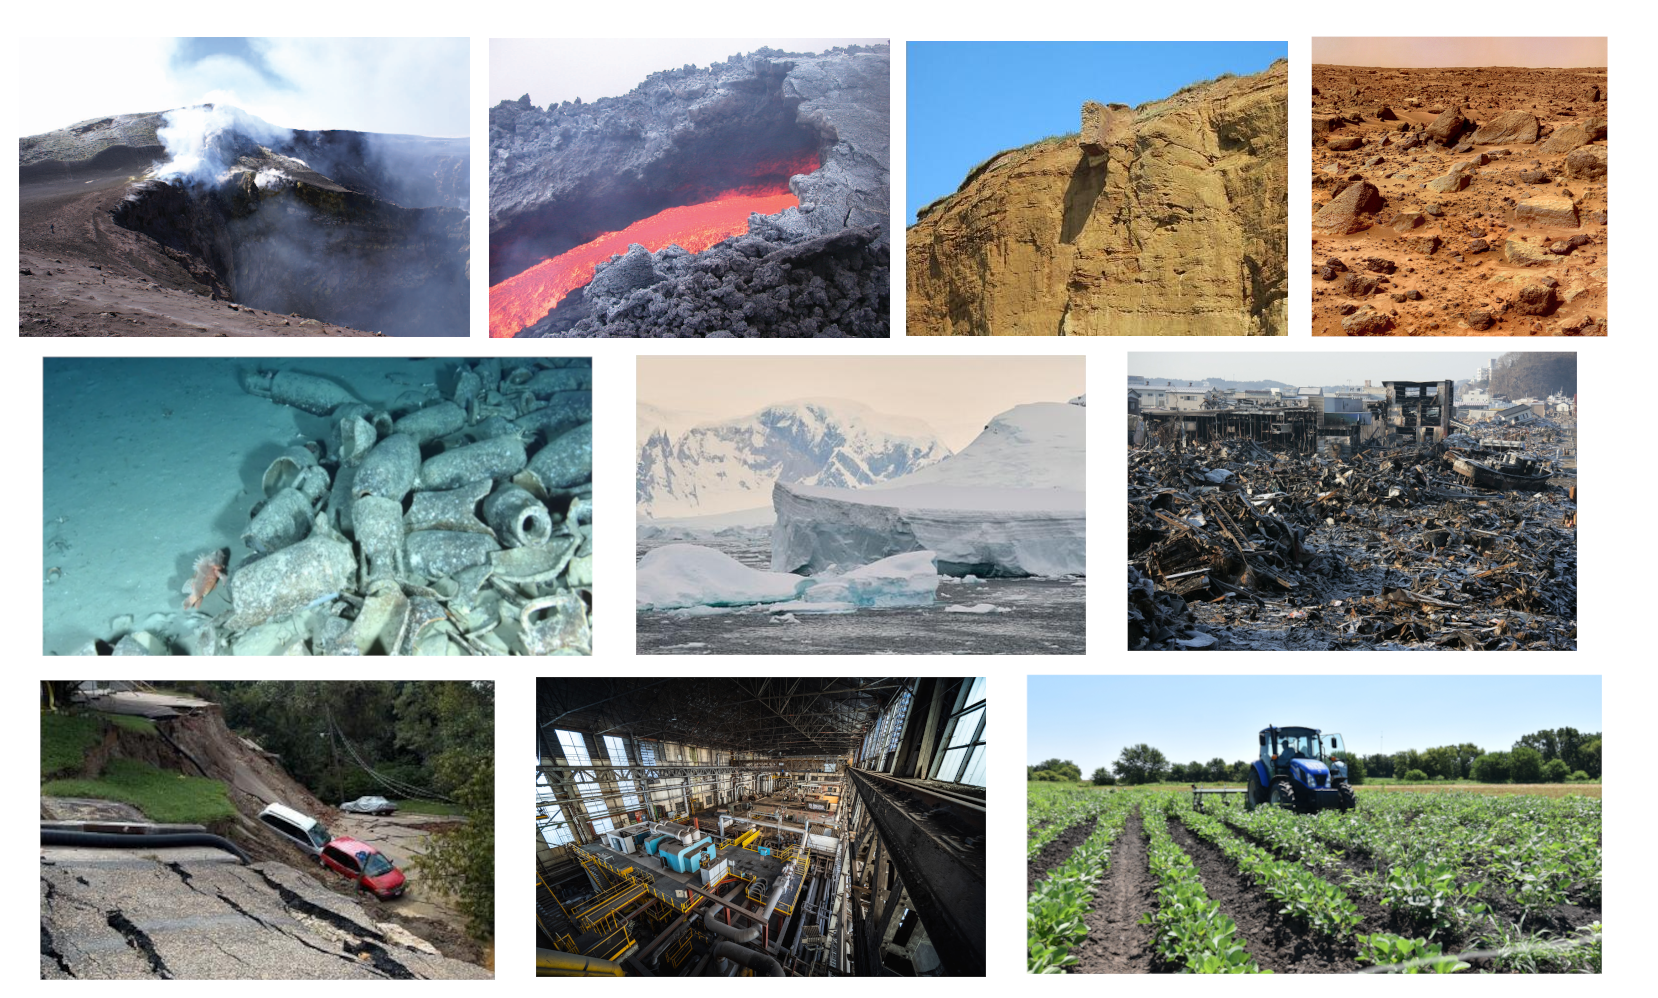
\includegraphics[width=0.85\textwidth]{Images/img_ch1/ExtremeUNstructured.png}
    \caption[Examples of unstructured and extreme environment]{Unstructured and extreme environment, in order from left to right and top to down: Mount Etna, Etna eruption, cliff, Mars, underwater archaeological site, Antarctica, Kasenumma city after the Great East Japan Earthquake, landslide,  power plant, farm field.}
    \label{fig:extreme_unstructured}
\end{figure}
Figure \ref{fig:extreme_unstructured} represents some examples of the domain of interest, referred to as \textbf{unstructured environments}. In particular, locations such as volcanoes, space, deep ocean, and disaster sites are referred to as \textbf{extreme environments}, and here more than in other places, the usage of autonomous systems is fundamental to complete different tasks\cite{Vulcanic_Survey}\cite{UnstructuredHOW}\cite{SearchandRescue}.

Extreme environments contain many rough 
terrains that limit the movement of robots, such as steep slopes, cliffs, and rubble areas, and depending on the robot's movement method, 
it may be impossible to reach the destination, or it may take a great deal of time and energy to reach the destination.
Therefore, designing robots for these critical areas is a complex task, involving not only material and electronics durability under extreme conditions, but also advanced 3D perception, environmental awareness, and adaptive locomotion strategies for efficient traversability\cite{TerrainTraversability}\cite{FieldRobots}.

This research focuses on environments composed of flat land and uneven terrain, as well as steeply sloping terrain made of rocks.
In the next section, the state-of-the-art robotics hardware is presented, to highlight the limitations of the classical approach, and introduce novel solutions, similar to the one discussed here. 

\section{Field Robots, different locomotions}
\label{sec:field_robots}
Autonomous and remotely operated machines working in unstructured environments are part of the \textbf{field robotics} research\cite{FieldRobots}. Here different cutting-edge systems are summarized and classified based on the type of locomotion solution.  


\subsection{Wheeled Robots}
\label{subsec:wheeled_robots}

Locomotion on wheels is the most common human transportation system, and the majority mobile robots are also based on this solution. Moving on wheels ensures high speed at low effort, and traversability can be improved with state-of-the-art suspension systems and mechanical structures. 

These types of robots are typically designed for flat terrains, with some robustness against possible roughness. Now some cutting-edge examples are presented.  

ECHO (see Fig.\ref{fig:ECHO}) is a four-wheeled robot to study emperor penguins' behavior, able to move in the Antarctic\cite{WHOI_ECHO} continent. Another example is
ROBOVOLC\cite{ROBOVOLC}\cite{Vulcanic_Survey}, represented in Fig.\ref{fig:ROBOVOLC}, is a robotic system moving on wheels even in rocky terrains, designed to help scientists in the exploration of volcanoes. 
As a final example, The 4-wheeled rover EX1 (in Fig.\ref{fig:EX1}) ensures smooth and stable driving at increased speed over loose soils, irregular hard surfaces, and hazard-abundant landscapes, thanks to its mechanically hybrid suspension system\cite{EX1}. 

\begin{figure}[H]
    \centering
    \subfloat[ROBOVOLC in mount Etna.\label{fig:ROBOVOLC}]{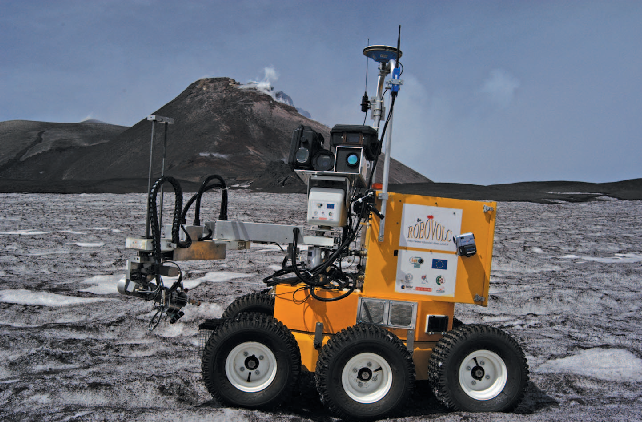
\includegraphics[width=0.28\textwidth]{Images/img_ch1/ROBOVOLC.png}}
    \subfloat[ECHO in Antartica.\label{fig:ECHO}]{
    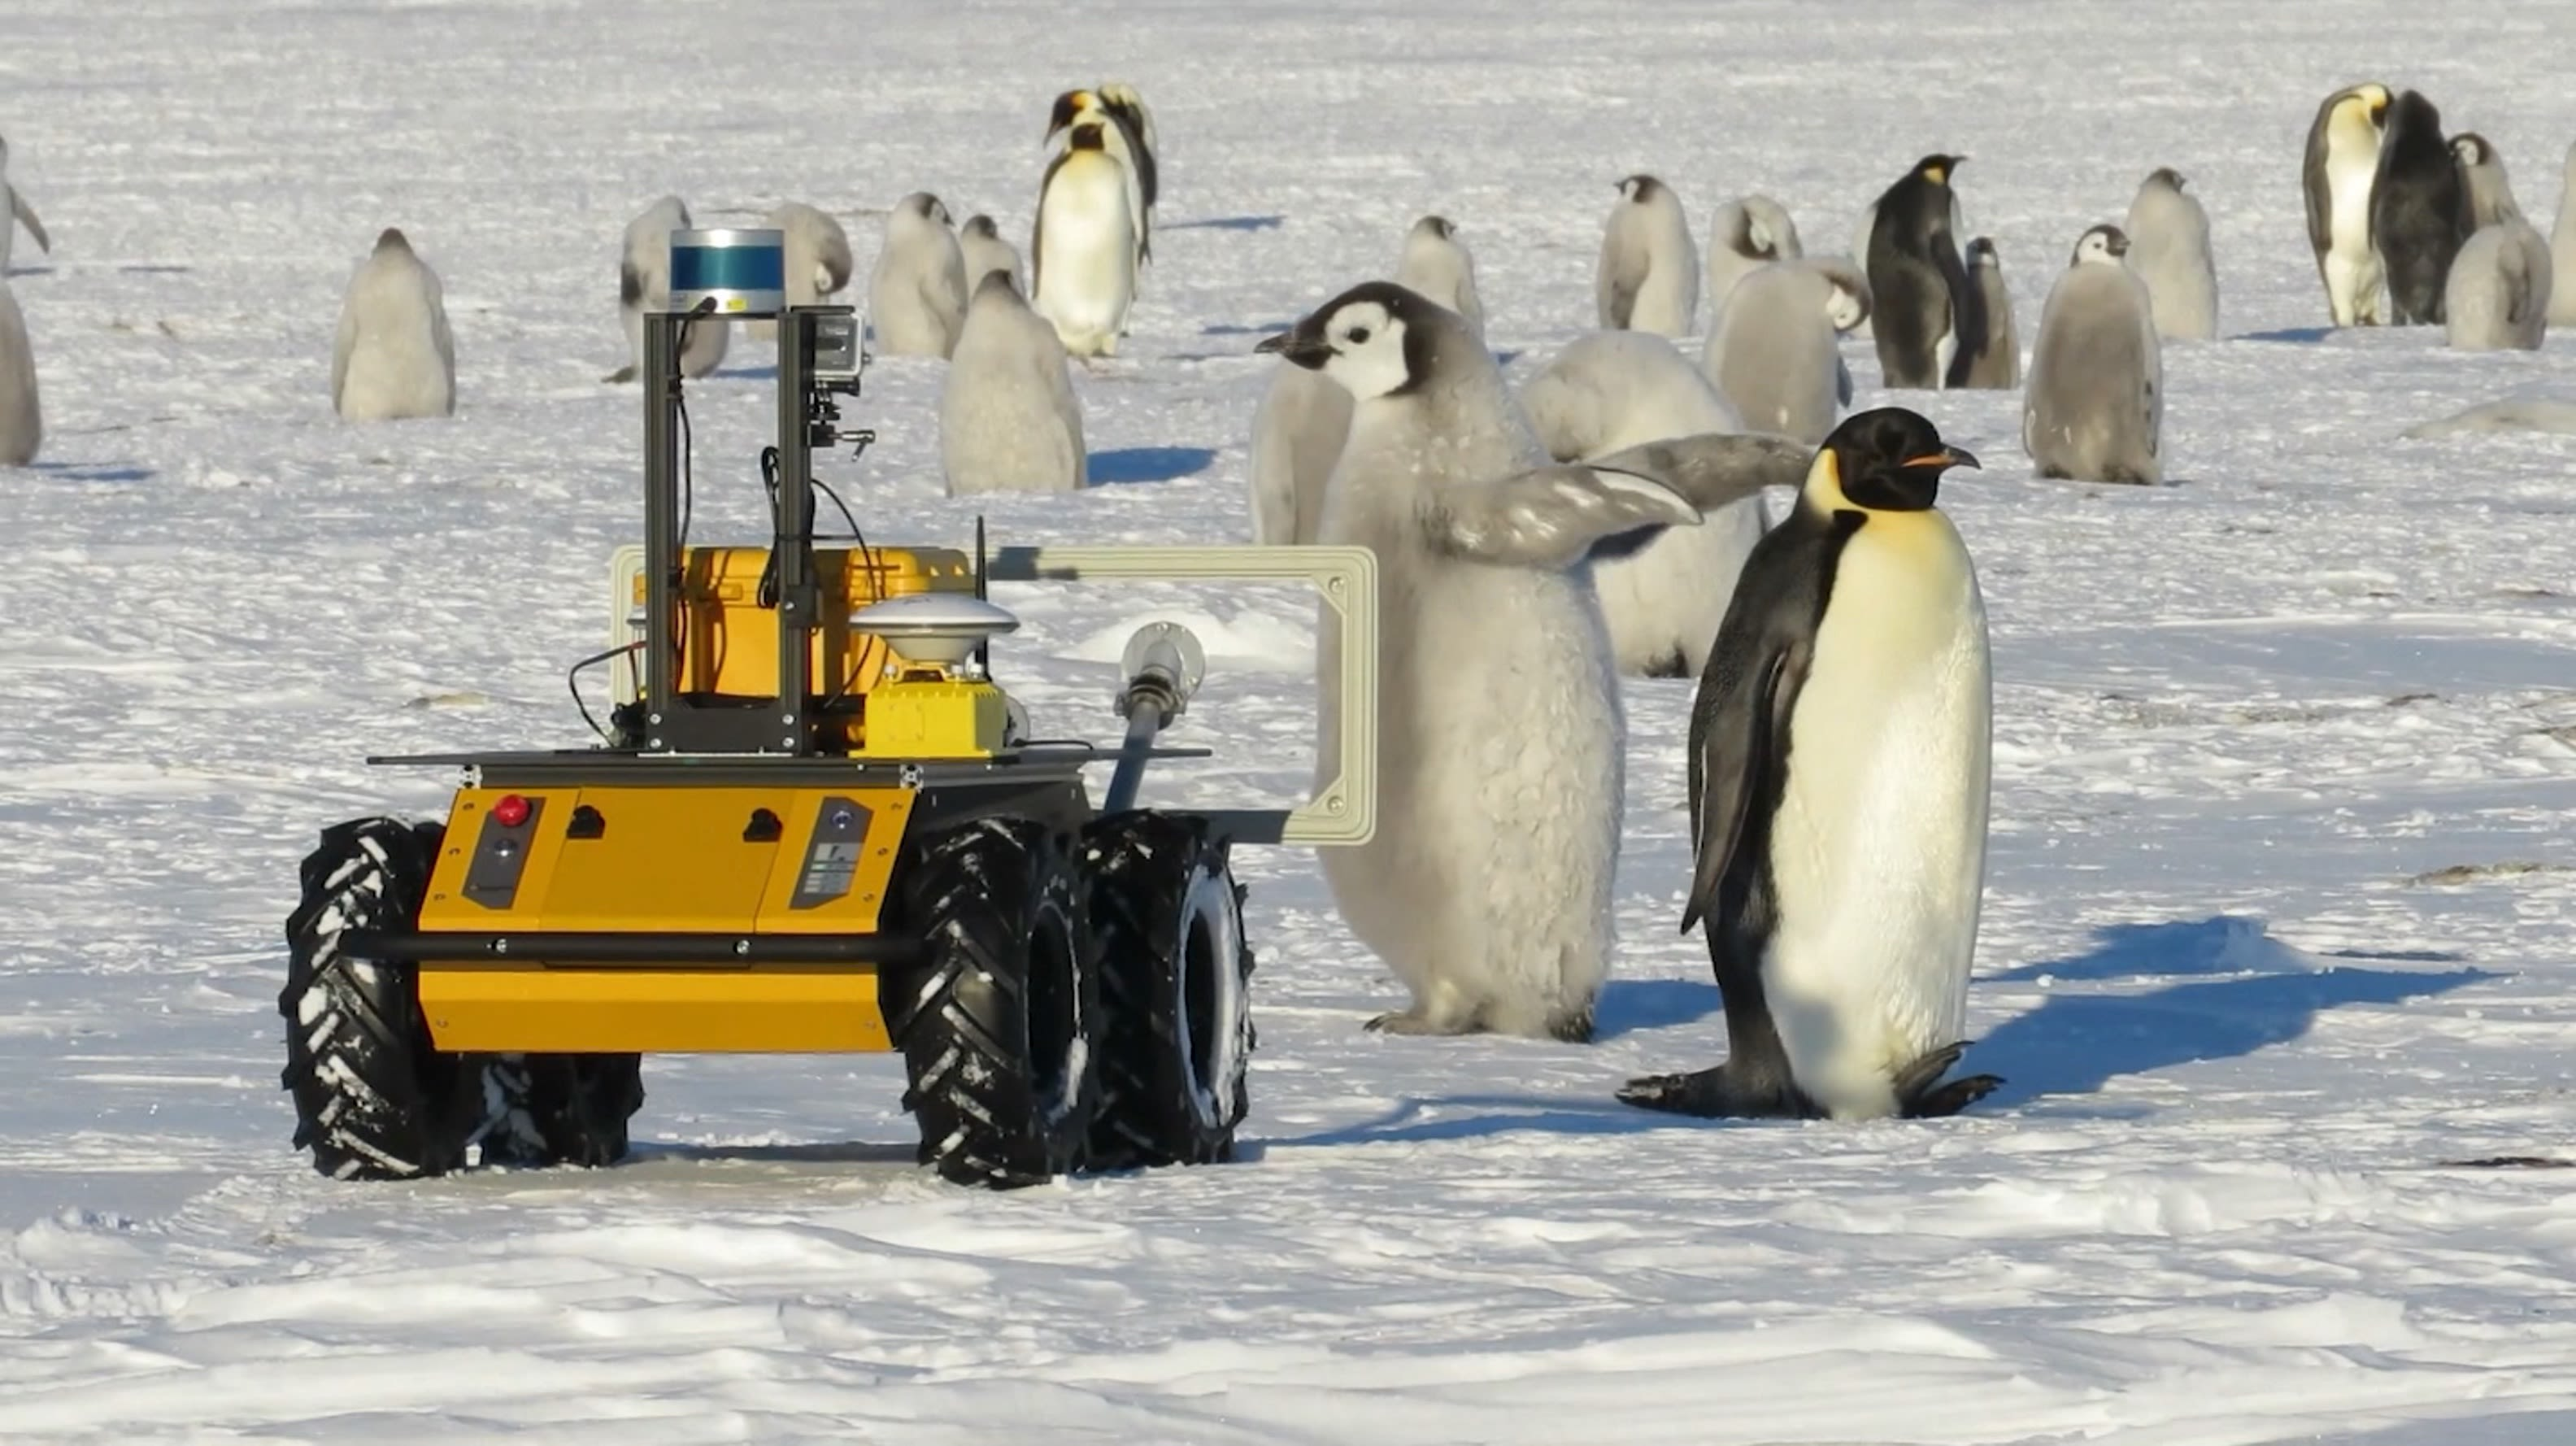
\includegraphics[width=0.32\textwidth]{Images/img_ch1/ECHO_antartica.jpg}}
    \subfloat[EX1 high-speed rover.\label{fig:EX1}]{
    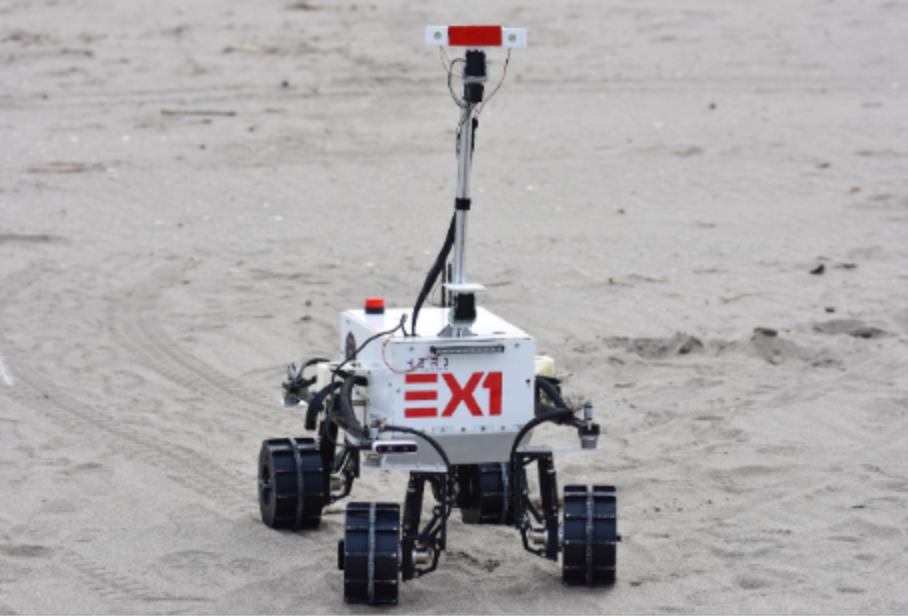
\includegraphics[width=0.28\textwidth]{Images/img_ch1/EX1.png}}
    \caption[Wheeled robot]{Wheeled robots}
    \label{fig:wheeled}
\end{figure}
The robots described here are different from other classical simple and rigid wheeled structure solutions. However, in muddy or very rough terrain, tracked locomotion is the most suitable.

\subsection{Tracked Robots}
\label{subsec:tracked_robots}

For their larger contact area with the ground,
tracked robots are used when high traction and payload capacity are required. 
Examples, represented in Fig.\ref{fig:tracked} are Quince \cite{Quince}\cite{FukushimaPlant}, a rescue robot developed by Satoshi Tadokor's group, and the tracked vehicles employed during the TRADR\cite{TRADR} project
\cite{Amatrice}\cite{SearchandRescue}. 

\begin{figure}[H]
    \centering
    \subfloat[Quince.\label{fig:WheelFly_robot}]{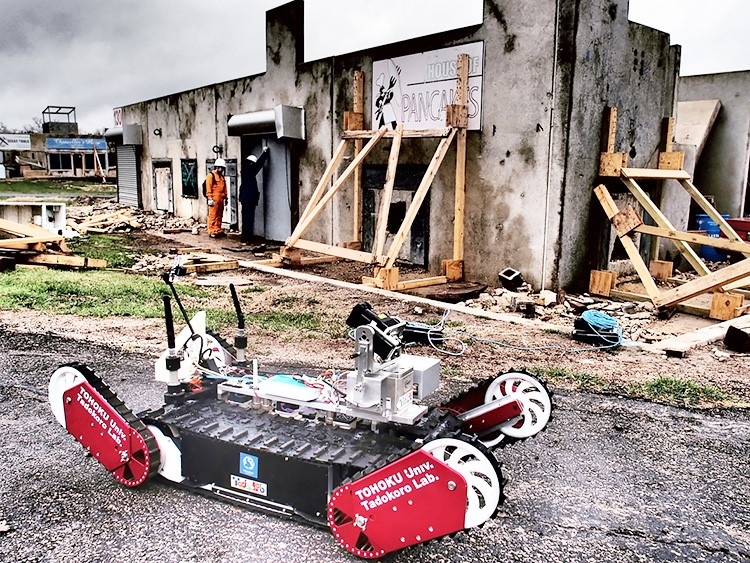
\includegraphics[width=0.4\textwidth]{Images/img_ch1/QuinceRobot.jpg}}
    \subfloat[rover form TRADR project, Amatrice.\label{fig:TRADR}]{
        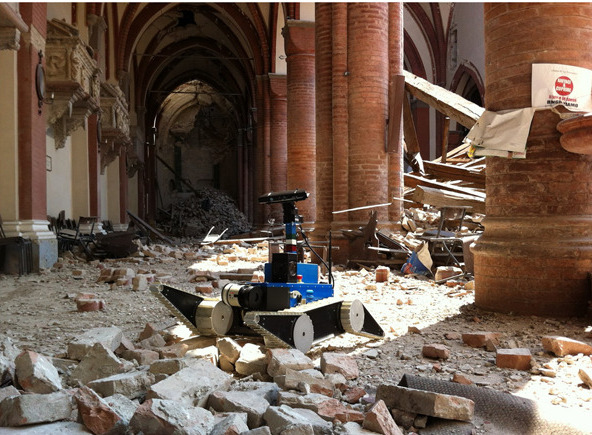
\includegraphics[width=0.4\textwidth]{Images/img_ch1/TRADR_UGV.jpg}}
    \caption[Tracked robots for search and rescue]{Tracked robots for search and rescue activities}
    \label{fig:tracked}
\end{figure}
With tracks, more types of terrains are traversable, at the cost of less energy efficiency than wheeled robots. 
However, there are still traversability limitations due to the required "continuous" trajectory on the ground, intrinsic both for tracked and wheeled locomotion. 


\subsection{Legged Robots}
\label{subsec:walking_robots}

The discrete ground interaction of legged robots solves
the problem mentioned above. This locomotion has been inspired by what Mother Nature has created over hundreds of millions of years of evolution and refinements\cite{Todd}.   

HyQ\cite{HyQ_website}\cite{HyQpaper} is a quadruped from the Italian Institute of Technology (IIT), ANYmal (in Fig.\ref{fig:ANYmal_outdoor} and \ref{fig:ANYmal_fire}), developed by ANYbotics for autonomous industrial inspection, and now enabling some of the most advanced legged locomotion capabilities 
\cite{LeggedRealWorld}\cite{AnymalDocThesis}\cite{LeggedRealWorld}\cite{SearchandRescue}.
Finally, from the researches on legged locmotion by Mark Raibert\cite{Raibert}, Boston Dynamics' Spot\cite{spot_website}  (in Fig.\ref{fig:Spot}) was one of the first machines to spark market interest in legged robots.
\begin{figure}[H]
    \centering
    \subfloat[ANYmal outdoor.\label{fig:ANYmal_outdoor}]{
        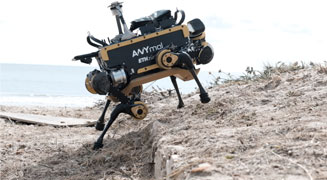
\includegraphics[width=0.3\textwidth]{Images/img_ch1/anymalOutdoor.png}
    }
    \subfloat[ANYmal during a fire.\label{fig:ANYmal_fire}]{
        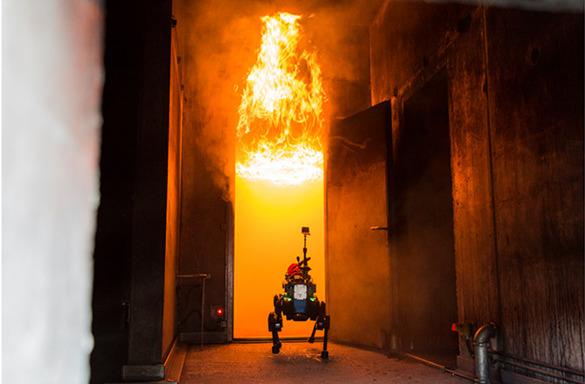
\includegraphics[width=0.3\textwidth]{Images/img_ch1/ANYmal_fire.jpg}
    }
    \subfloat[Boston Dynamics Spot.\label{fig:Spot}]{
        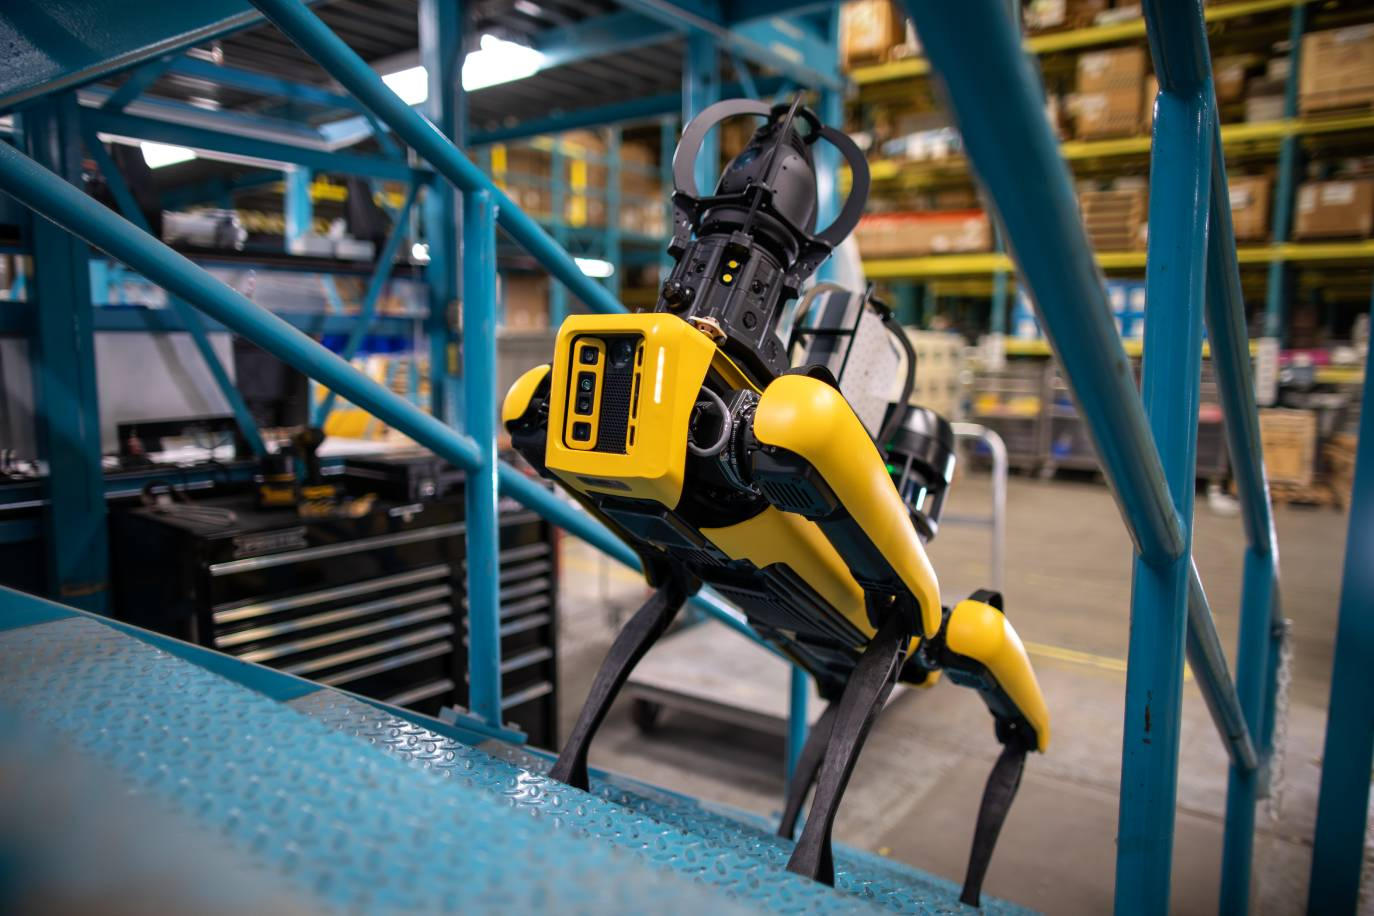
\includegraphics[width=0.3\textwidth]{Images/img_ch1/Spot.jpg}
    }
    \caption[Quadruped legged robots]{Examples of quadruped legged robots in unstructured environment.}
    \label{fig:WalkingRobots}
\end{figure}
The higher terrain adaptability again comes with costs in terms of energy efficiency and much more complexity in the development and design of those systems. 

Bipedal, hexapod, and even octopod legged robots exist, and it is relevant to highlight the increase of payload and stability when using more legs, and the manipulation ability with two upper arms in humanoids\cite{HumanoidRobot}.

The concept of legged locomotion can be extended into limbed robots, which use their "limbs" to move the base and manipulate the environment, without having to differentiate arms and legs as humanoid does.  

\subsection{Multilimb Robots}
\label{subsec:multilimb_robots}

Multilimbed robots are a wide class of robots\cite{Koyachi}, and legged machines are a subclass of this. 
Classical walking machines use simple foot tips and specific leg structures to interact with the environment and generate the necessary reaction forces to achieve motion. Multilimbed machines instead can employ different types of end effectors attached at the limb-end, depending on the task, such as magnetic modules \cite{MAGNEKO}, vacuum suction units\cite{suctionfoottip}, and passives spine grippers\cite{passiveSpineTohoku}, to list a few possibilities.
Furthermore, the limbs are properly structured to enhance the workspace, and sometimes redundant designs are employed. 

Particular types of multilimbed machines are climbing robots, designed to move on high slopes, vertical surfaces, or even on the ceiling. An example is the JPL/NASA LEMUR3 robot\cite{LEMUR3} (see Fig.\ref{fig:LEMUR3}), enabling access to previously inaccessible but scientifically relevant areas for space missions. In general, climbing robots lose performance when walking on the ground because designed for optimized climbing locomotion,  
SCALER\cite{SCALER} instead, guarantees fast locomotion also on the ground, and a new gait using the reconfigurable base, as represented in Fig.\ref{fig:SCALER}
\begin{figure}[H]
    \centering
    \subfloat[LEMUR3.\label{fig:LEMUR3}]{
    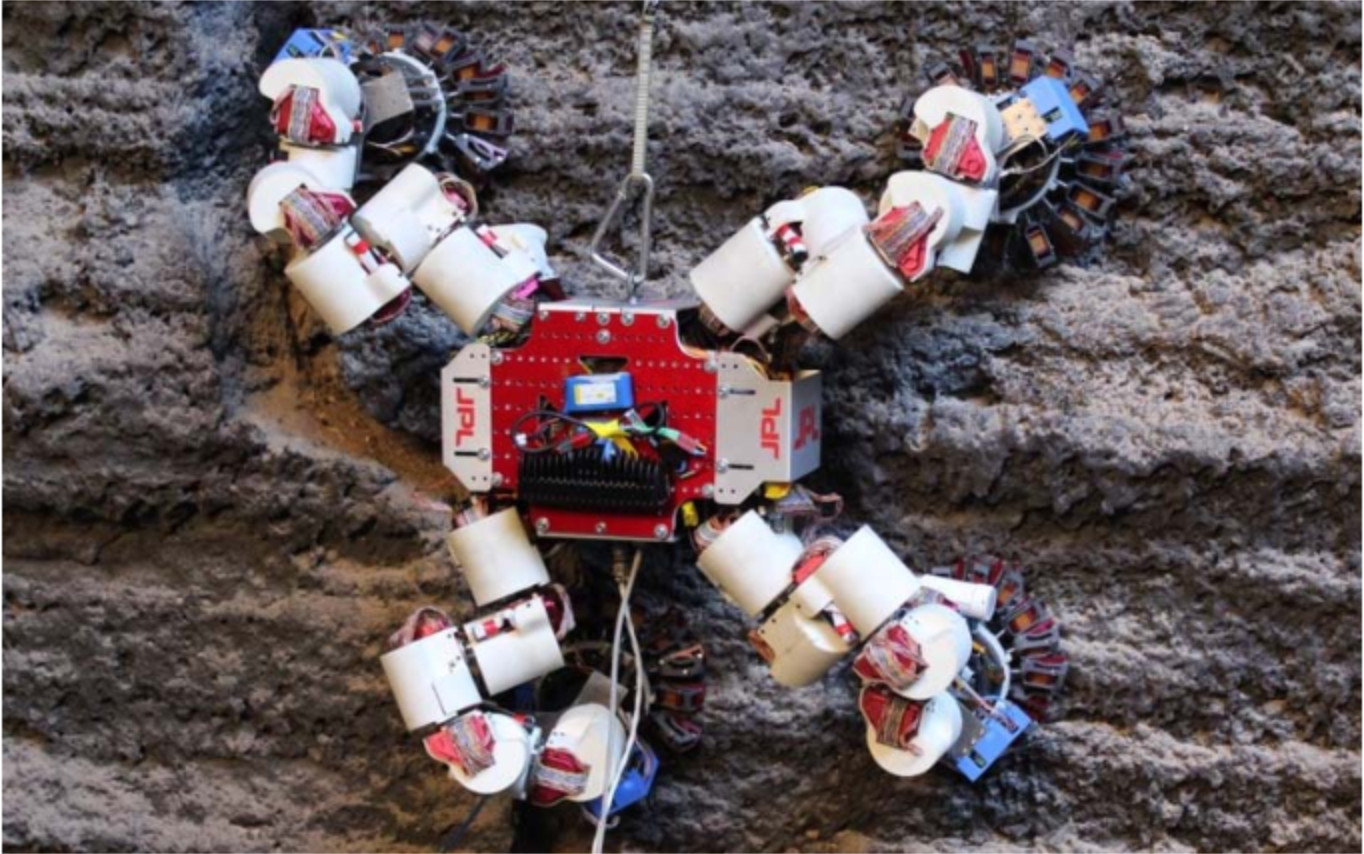
\includegraphics[width=0.55\textwidth]{Images/img_ch1/LEMUR3.png}}
    \subfloat[SCALER.\label{fig:SCALER}]{
    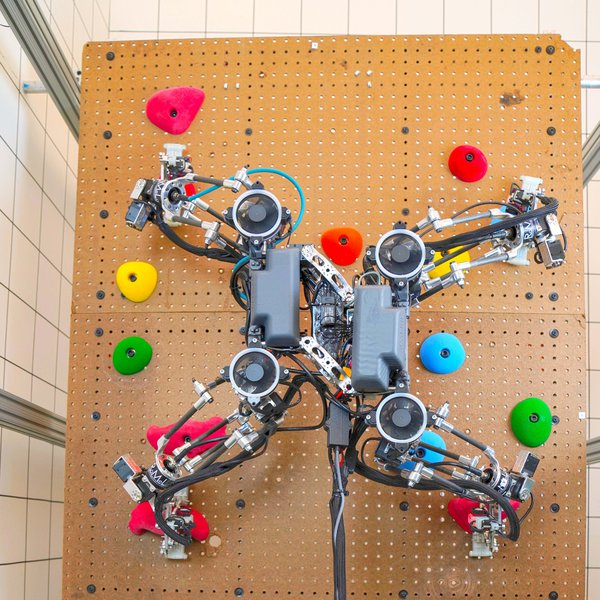
\includegraphics[width=0.35\textwidth]{Images/img_ch1/SCALER.jpg}}  
    \caption[Multi-Limb climbing robots]{Multi-limb climbing robots.}
    \label{fig:Climbing}
\end{figure}
An example of a multifunctional multilimbed robot is SCAR-E, an omnidirectional hexapod designed by the team of the Asteroid Mining Corporation (AMC). This robot structure enables horizontal and vertical locomotion in uneven environments, and multiple task execution with an interchangeable end effector\cite{SCARE_gripper}\cite{SCAR-E}. Figure \ref{fig:SCARE} represents the robot with simple feet and the designed soft gripper for its mission. Furthermore, the increased workspace of the limb allows it to reach tools carried on the base, and change the end effector depending on the task.

\begin{figure}[H]
    \centering
    \subfloat[SCAR-E Concept.\label{fig:SCARE_Concept}]{
        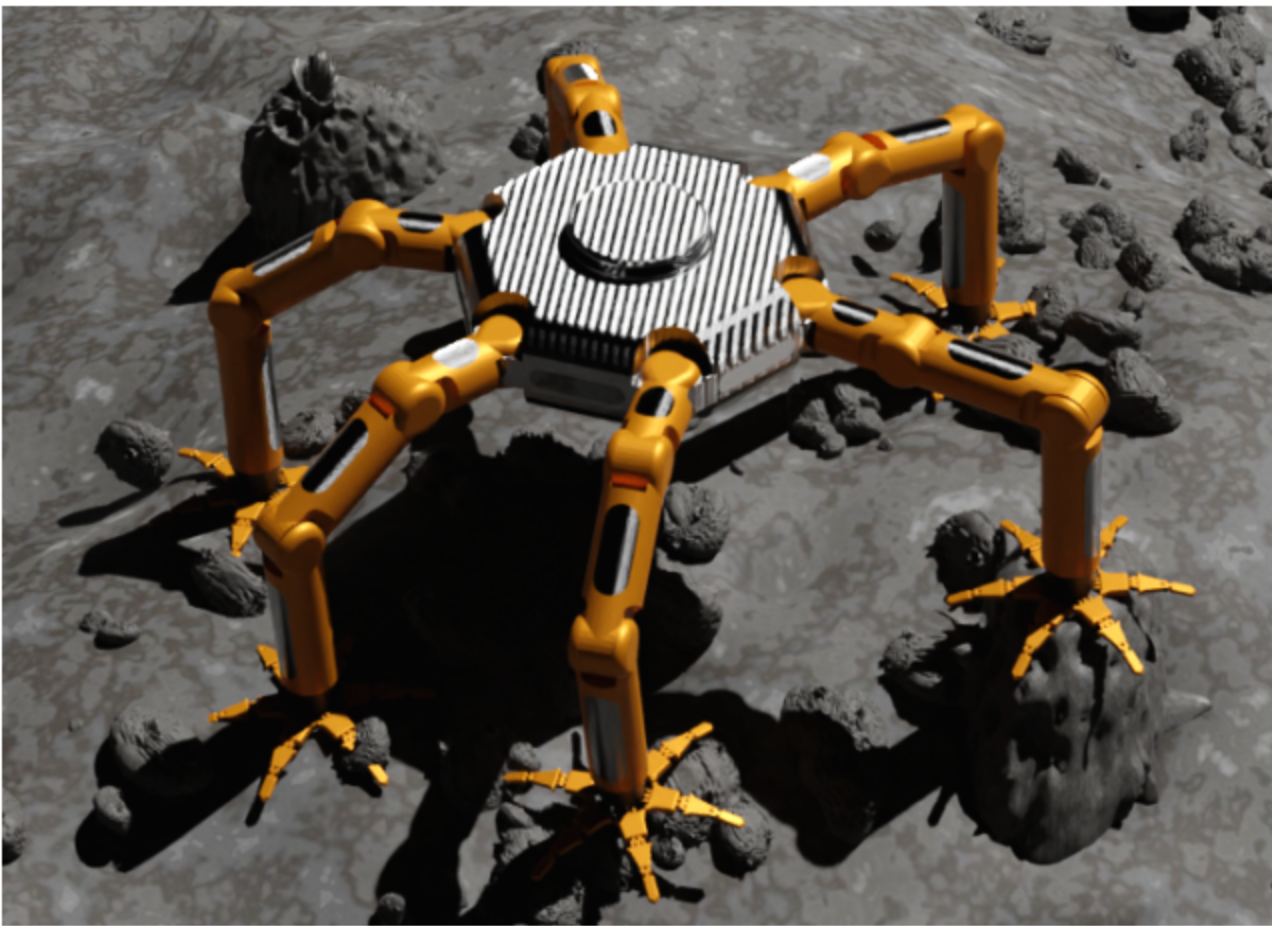
\includegraphics[scale=0.13]{Images/img_ch1/SCAR-E_concept.png}
    }
    \subfloat[SCAR-E Multi-limb Robot.\label{fig:SCARE_Robot}]{
        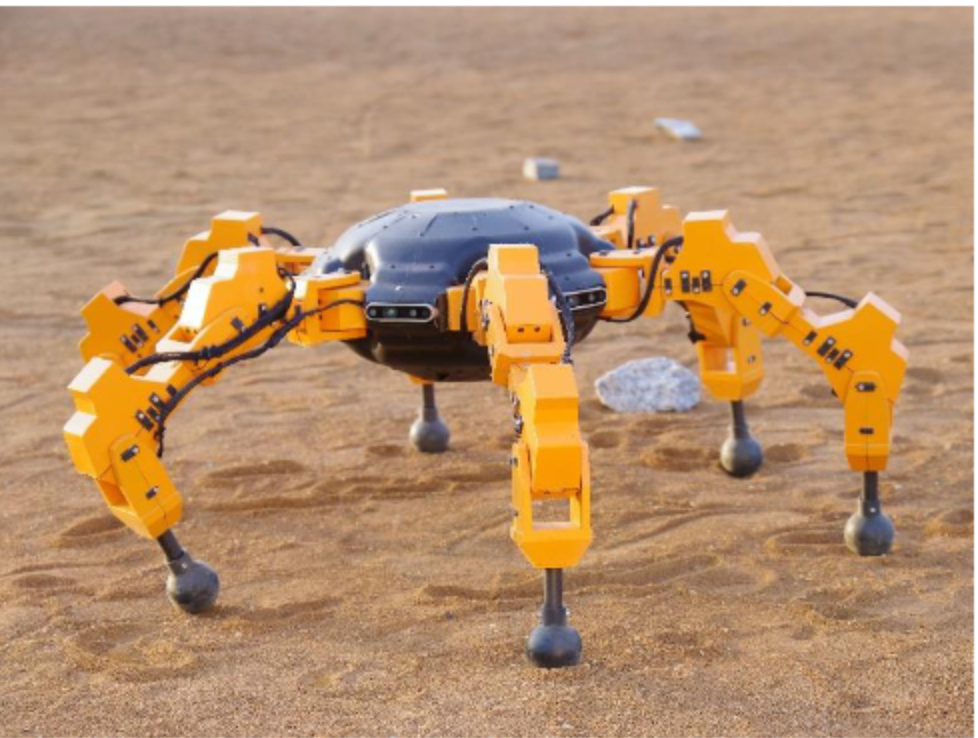
\includegraphics[scale=0.18]{Images/img_ch1/SCAR-E.png}
    }
    \subfloat[Soft gripping system.\label{fig:SCARE_Gripper}]{
        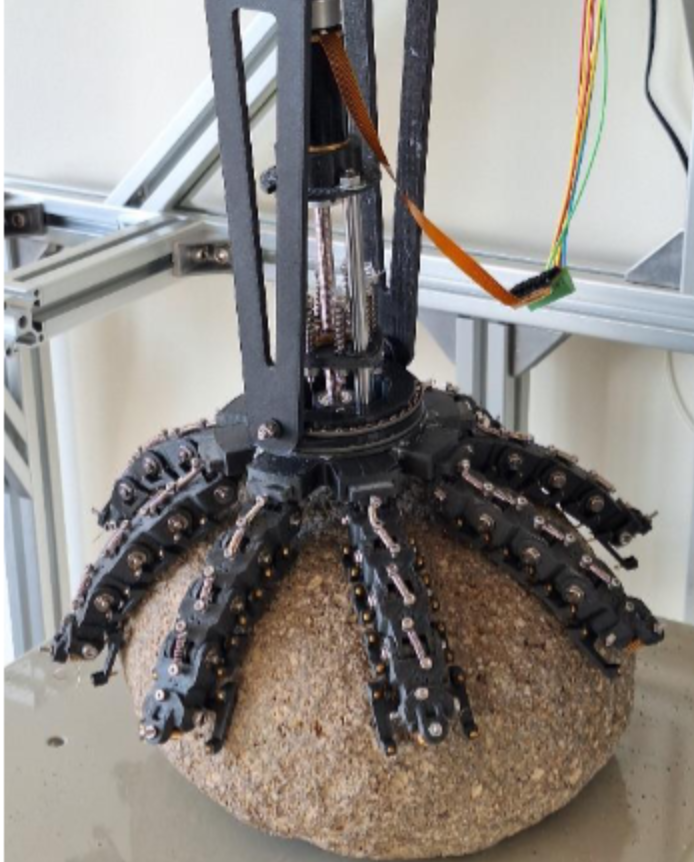
\includegraphics[scale=0.15]{Images/img_ch1/SCAR-E_Gripper.png}
    }
    \caption[Asteroid Mining Corporation (AMC) SCAR-E.]{AMC SCAR-E multi-limb robot for asteroid mining\cite{SCARE_gripper}\cite{SCAR-E}.}
    \label{fig:SCARE}
\end{figure}


Other locomotion solutions exist for other domains, such as propellers and thrusters for air and underwater navigation, enabling flying and swimming locomotion.
The problem with flying systems is that in general narrow navigation is complex, the cost of hovering is non-negligible, and payload capabilities are limited. 

Table \ref{table:locomotion_summary} summarizes the performance of the different classical locomotion forms as an average of traversability and energy efficiency.

\begin{table}[H]
\centering 
    \caption{Summary of locomotion performances for different terrains and tasks, where the average performance is measured from 0 to 3}
    \label{table:locomotion_summary}
    \begin{tabular}{ c }
    \textbf{Limb Joints Motors}
    \end{tabular}
    \begin{tabular}{| c | c | c | c | c | c |}
    \hline
    \rowcolor{bluepoli!40}
%    \rowcolor{bluepoli!40}
     \textbf{Task} &  Wheeled & Tracked & Walking & Climbing & Flying\T\B \\
    \hline \hline
    \textbf{Flat Terrains} & \cellcolor{bluepoli!20}3 & 2 & 1 & 0  & 2  \T\B\\
    \hline 
    \textbf{Rough Terrains} & 0 & 2 & \cellcolor{bluepoli!20}3 & 1  & 2 \T\B\\
    \hline
    \textbf{Rocky Slopes} & 0 & 1 & 1 & \cellcolor{bluepoli!20}3 & 2 \T\B\\
    \hline
    \textbf{Vertical Walls} & 0 & 0 & 0 & \cellcolor{bluepoli!20}3 & 2 \T\B\\
    \hline
    \textbf{Manipulation} & 0 & 0 & 0 & \cellcolor{bluepoli!20}3 & 0 \B\\
    \hline
    \end{tabular}
\end{table}


In conclusion, for the complex terrain considered in this research, which includes sloping rocky surfaces, flat ground, and uneven terrain, none of the proposed solutions achieve the optimal balance between energy efficiency and mobility.
To solve the issue of adaptability to different terrain conditions, without sacrificing efficiency or speed, hybrid forms of locomotion and multimodal robot designs exist. 

\subsection{Hybrid and Multimodal Robots}
\label{subsec:hybrid_robots}

The combination of multiple forms of locomotion is an active research topic, from the cooperation of more robots
\cite{MultimodalityROBOTS}, to the possibility of integrating multiple functionalities on a single machine.

Focusing on single-agent systems, 
In literature, the terms hybrid and multimodal are often used interchangeably, here the following differentiation is considered:\\ 
\textit{The locomotion is considered \textbf{hybrid} when a non-conventional solution enables multiple interactions with the environment, based on the same mechanism. \textbf{Multimodality}, on the other hand, involves different forms of movement from multiple integrated actuators, or a reconfiguration of the system structure.}

First, some examples from the hybrid locomotion domain are presented. 

The hybrid form of ANYmal\cite{AnymalDocThesis}\cite{legged-wheeled} (in Fig.\ref{fig:ANYmal_Wheels}) uses non-steerable wheels attached to its legs, allowing the robot to be efficient
on flat as well as agile on challenging terrain. Furthermore, it exploits skating motions with passive wheels, 
reducing the cost of transport
from legged systems. MAMMOTH\cite{MAMMOTH}\cite{MAMMOTH_structure} (in Fig.\ref{fig:MAMMOTH}) is an actively articulated wheel-on-leg rover, capable of traversing obstacles while driving, by reconfiguring its legs. Another example is Q-Whex\cite{QWhex}, a quasi‐wheeled hexapod robot (represented in Fig.\ref{fig:QWhex}), which uses a unique wheel design to traverse different types of irregular terrains. 


\begin{figure}[H]
    \centering
    \subfloat[ANYmal hybrid locomotion\label{fig:ANYmal_Wheels}]{
        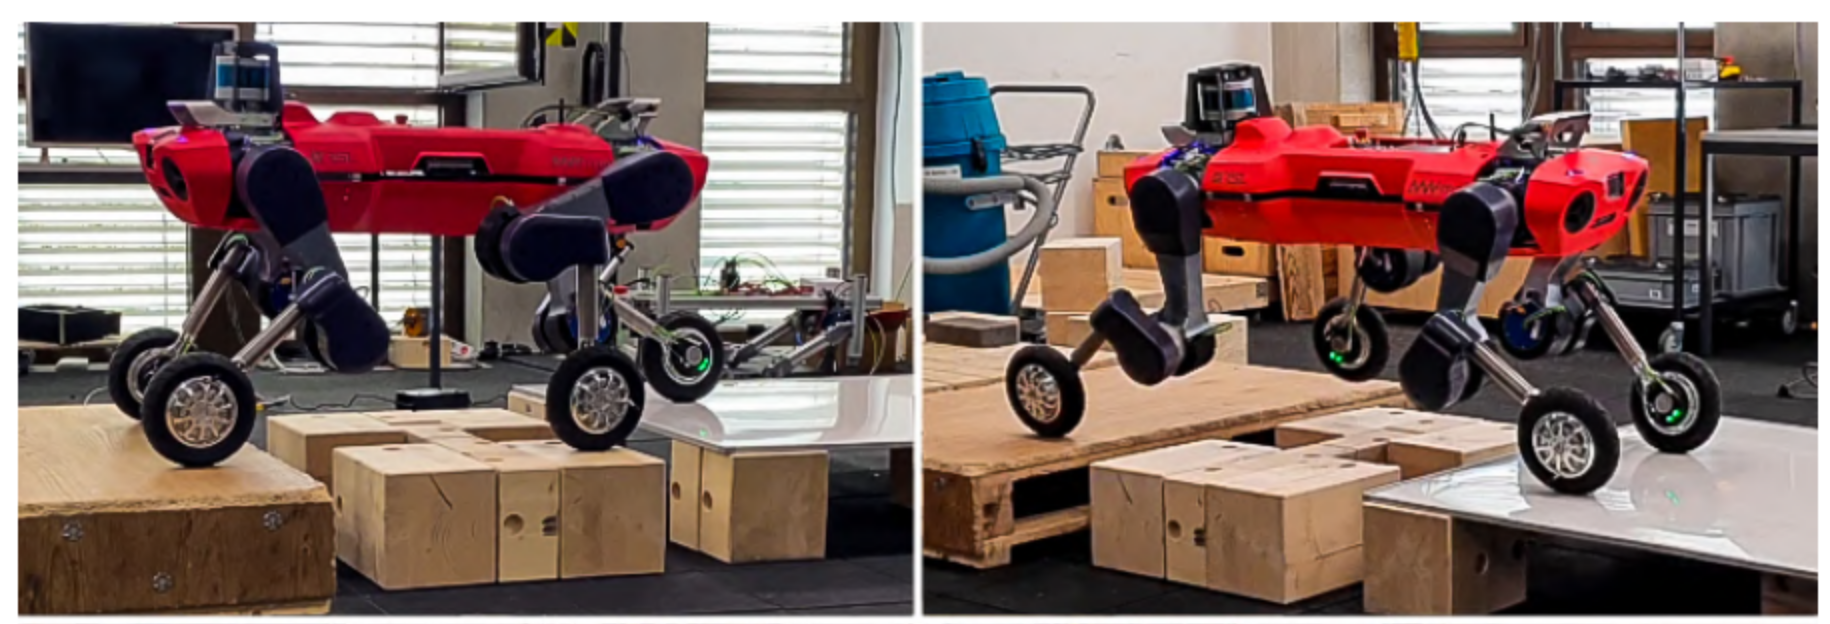
\includegraphics[width=0.50\textwidth]{Images/img_ch1/ANYmal_wheels.png}}
    \subfloat[MAMMOTH\label{fig:MAMMOTH}]{
        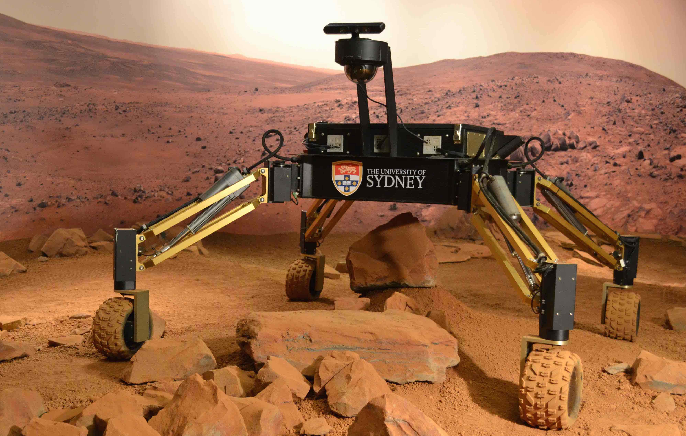
\includegraphics[width=0.25\textwidth]{Images/img_ch1/MAMMOTH.png}}
    \subfloat[Q-Whex \label{fig:QWhex}]{
        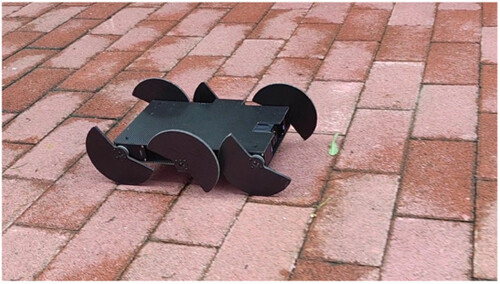
\includegraphics[width=0.25\textwidth]{Images/img_ch1/Q_Whex_quasiWheel.jpg}}
    \caption[Hybrid locomotion examples]{Hybrid locomotion robots examples}
    \label{fig:HybridLeggedWheel}
\end{figure}

The hybrid locomotion solutions described above use particular mechanical structures and adaptability behavior to enhance locomotion, 
when the robot reconfigures its mechanical structure or uses completely different actuators for different motion tasks, it is considered multimodal.

Multi-Modal Mobility Morphobot, or M4\cite{WheelFly} (represented in Fig.\ref{fig:WheelFly}), employs its components in different ways as wheels, thrusters, and legs, and simulates animals' behavior to enable extensive locomotion plasticity.
Examples of robots that remain on the ground are the reconfigurable legged-tracked AZIMUT\cite{LegsTracks_Azimut}
and the prototype legged-wheeled hexapod robot\cite{Hexapod_LegWheeled}, represented in Fig.\ref{fig:LegMultimodal}.
These two robots reconfigure their mechanical structure to change the ground interaction, furthermore, the hexapod prototype has manipulation capabilities thanks to the additional stability derived from using more legs. 

\begin{figure}[H]
    \centering
    \subfloat[Wheel mode.\label{fig:WheelFly_robot}]{
        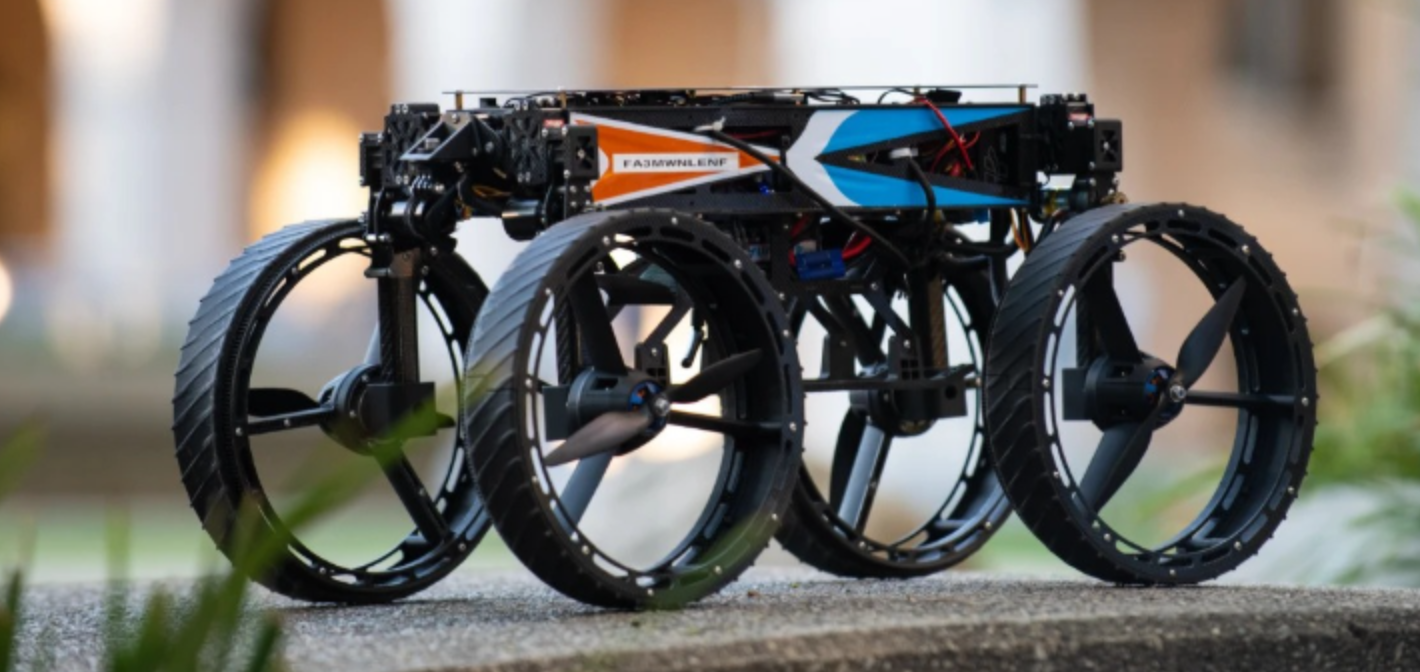
\includegraphics[width=0.4\textwidth]{Images/img_ch1/WheelFly_robot.png}}
    \subfloat[Locomotion transformation seqence.\label{fig:WheelFly_transformation}]{
        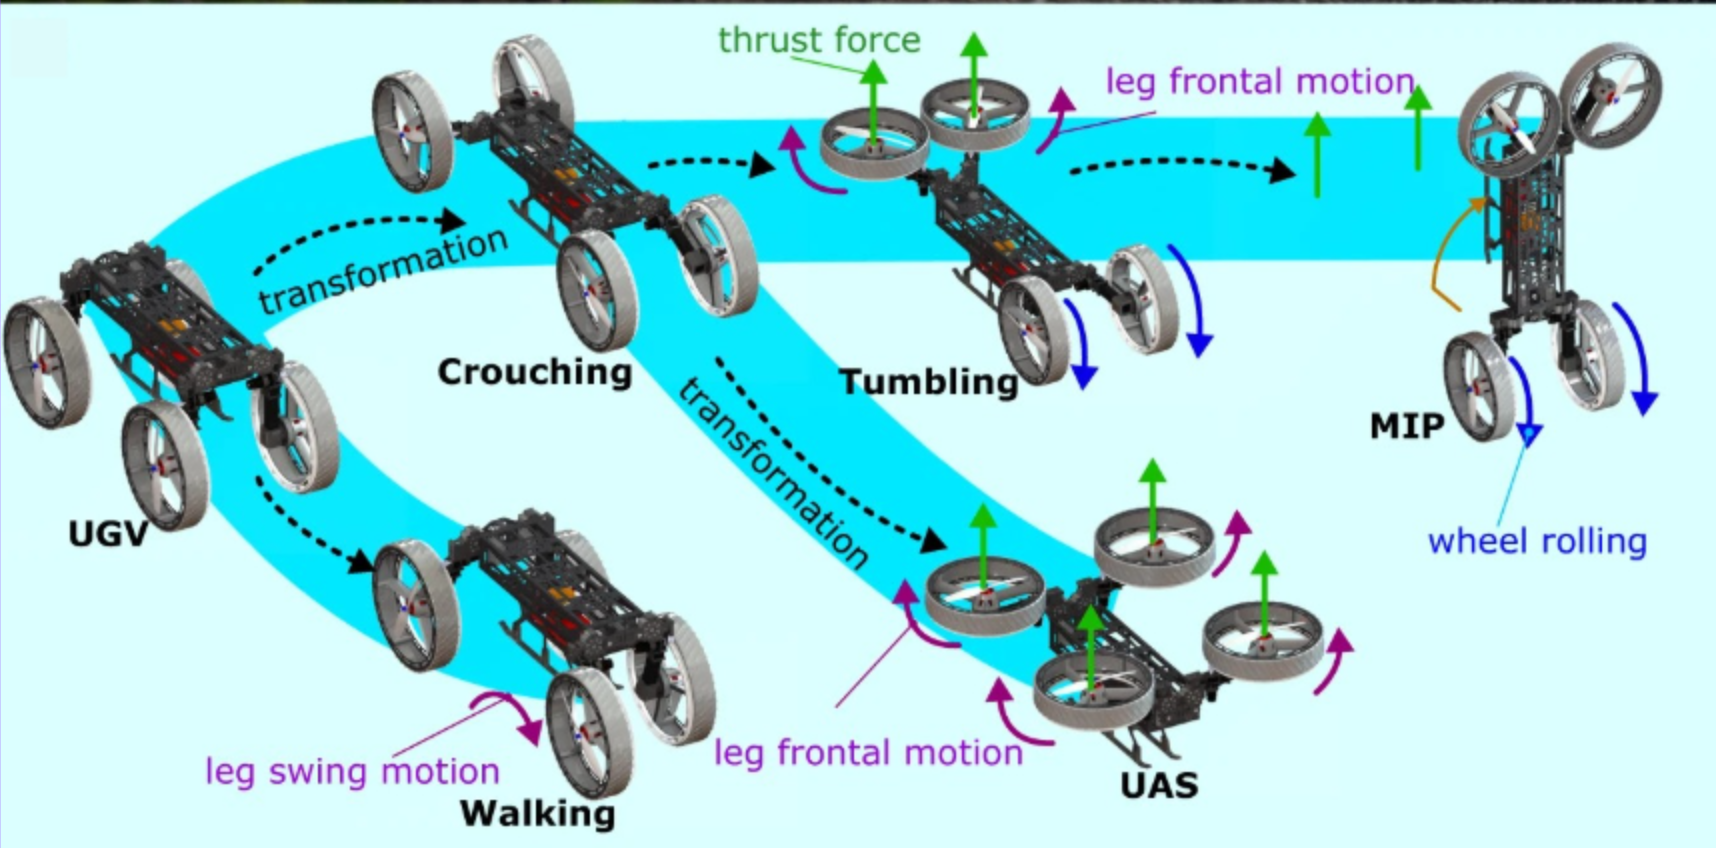
\includegraphics[width=0.55\textwidth]{Images/img_ch1/WheelFly_transformation.png}}
    \caption[Morphobot, driving-flying robot]{Morphobot \cite{WheelFly}, a multimodal driving-flying robot}
    \label{fig:WheelFly}
\end{figure}

\begin{figure}[H]
    \centering
    \subfloat[legged-wheeled hexapod.\label{fig:hexapod_Legwheels}]{
        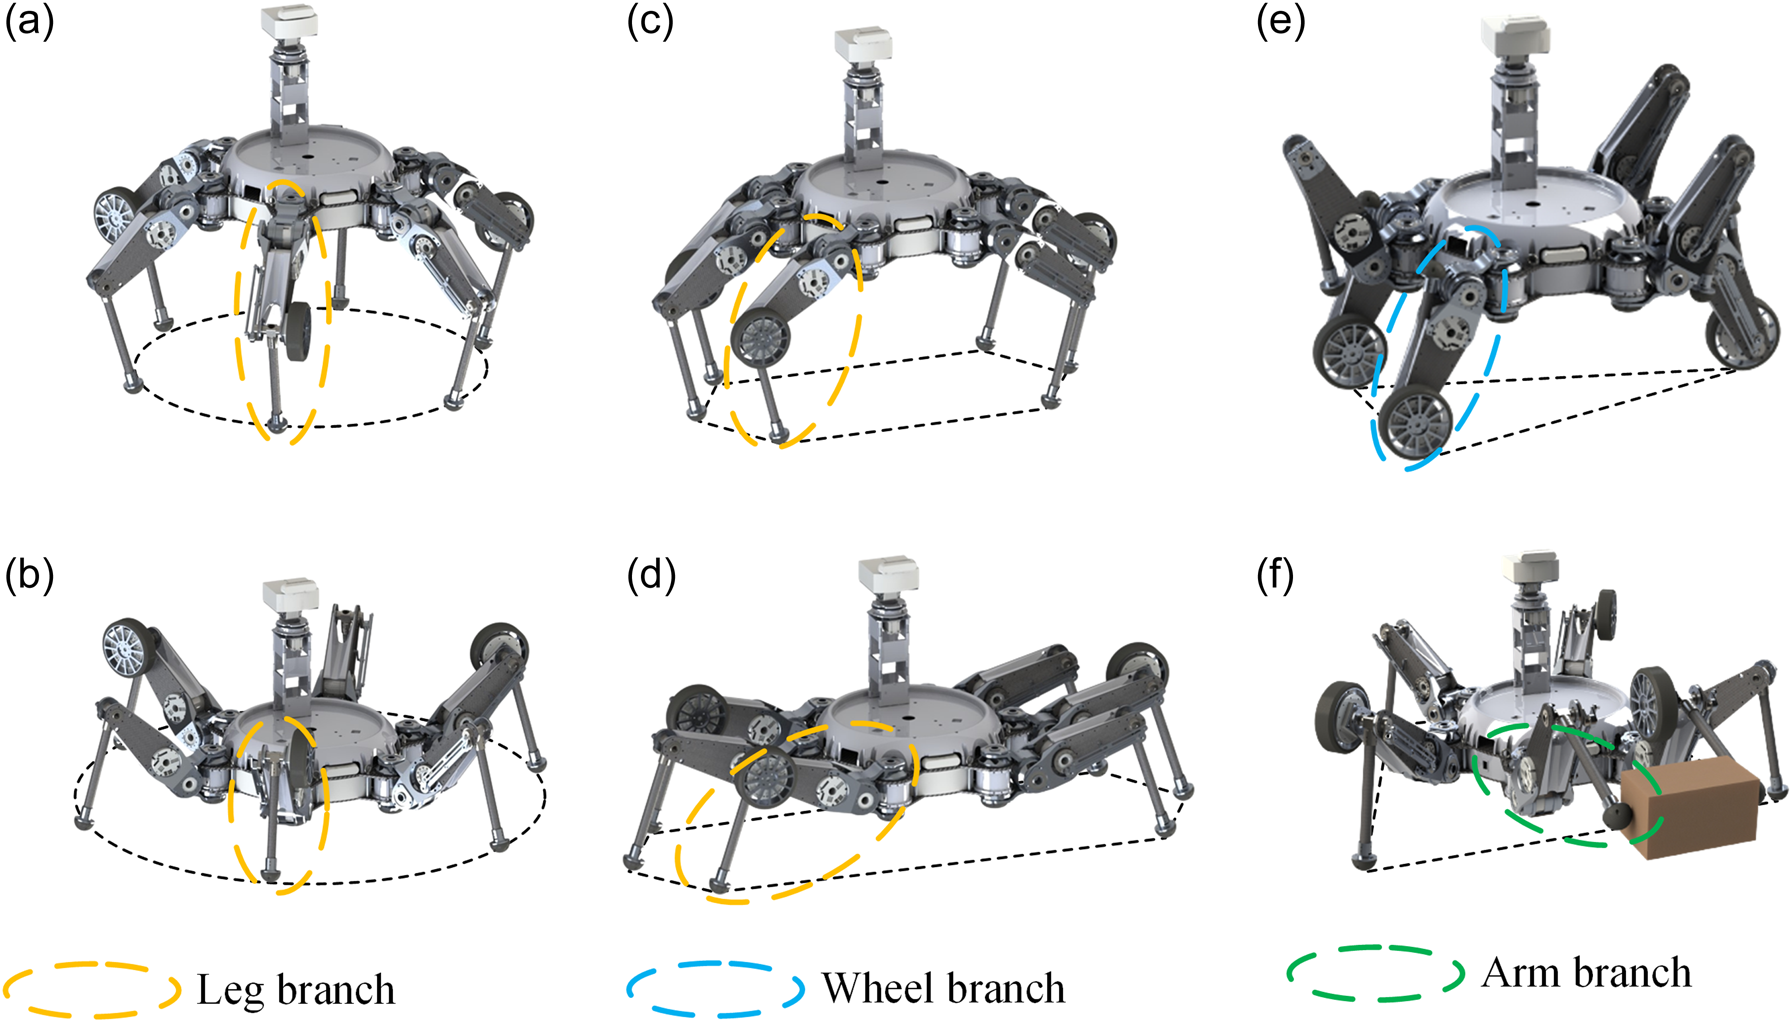
\includegraphics[width=0.6\textwidth]{Images/img_ch1/hexapod_Legweheels.png}}
    \subfloat[legged-tracked AZIMUT.\label{fig:AZIMUT}]{
        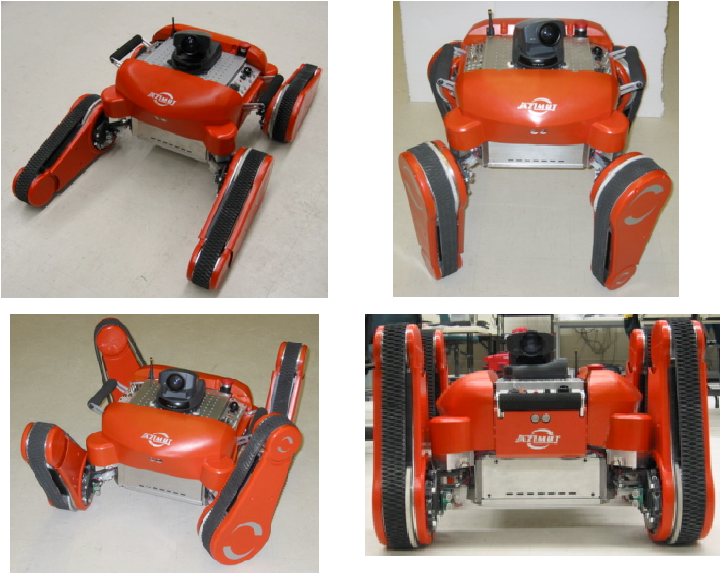
\includegraphics[width=0.4\textwidth]{Images/img_ch1/AZIMUT.png}
    }
    \caption[Multimodal legged robots]{Multimodal robots with different locomotion cpabilities}
    \label{fig:LegMultimodal}
\end{figure}

A cutting-edge robotic system for disaster response is the WAREC-1\cite{WAREC_Site} (and its successor 1R\cite{WAREC1R}), developed from the cooperation of different Japanese research institutes as part of the ImPACT project\cite{JST_IMPACT}. This four-limbed robot has advanced locomotion and manipulation capabilities\cite{WAREC1R_drilling}, transitioning among various locomotion styles, from bipedal/quadrupedal walking, crawling, ladder climbing\cite{WAREC1_book}\cite{WAREC1R}, and even driving with steerable or mecanum wheels.    
Figure \ref{fig:WAREC1} reports the possible manipulation and locomotion capabilities, even in highly unstructured environments with complex tasks to complete and obstacles to traverse. 

\begin{figure}[H]
    \centering
    \subfloat[Manipulation \label{fig:WAREC_manipulation}]{
    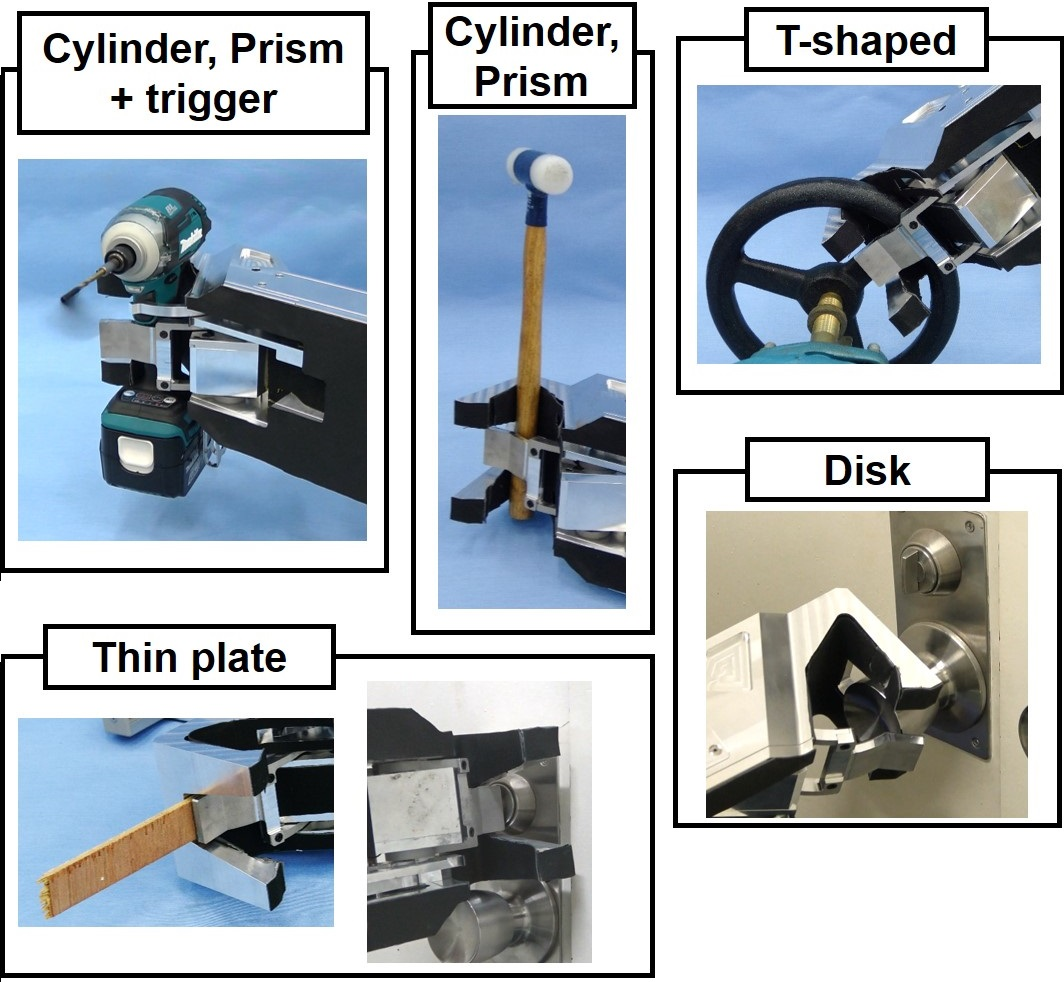
\includegraphics[width=0.3\textwidth]{Images/img_ch1/EE_WAREC1.jpg}}
    \subfloat[Omni wheel end effector\label{fig:WAREC_omniwheel}]{
    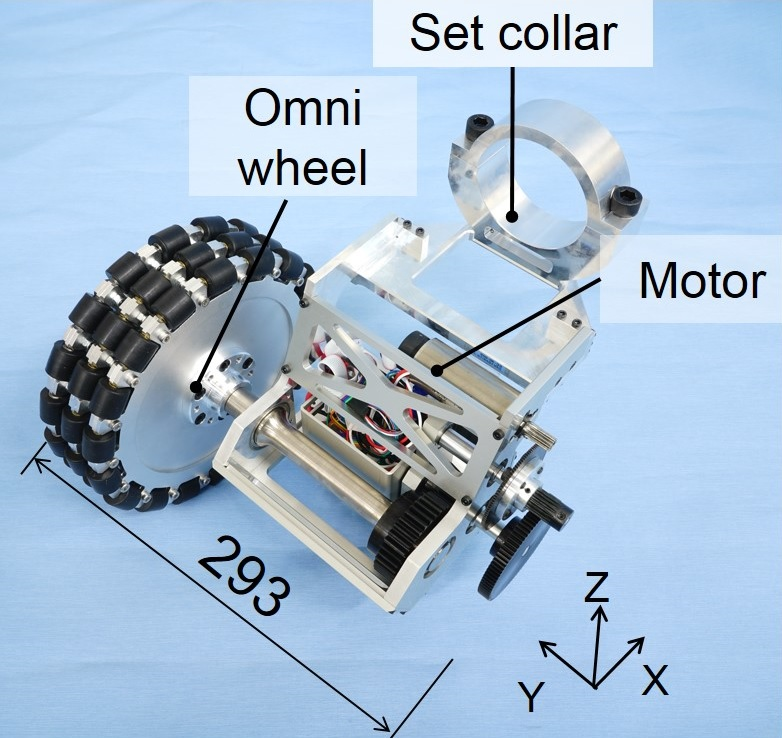
\includegraphics[width=0.3\textwidth]{Images/img_ch1/omniwheel_WAREC1.jpg}}
    \subfloat[Omni wheel driving mode \label{fig:WAREC_driving}]{
    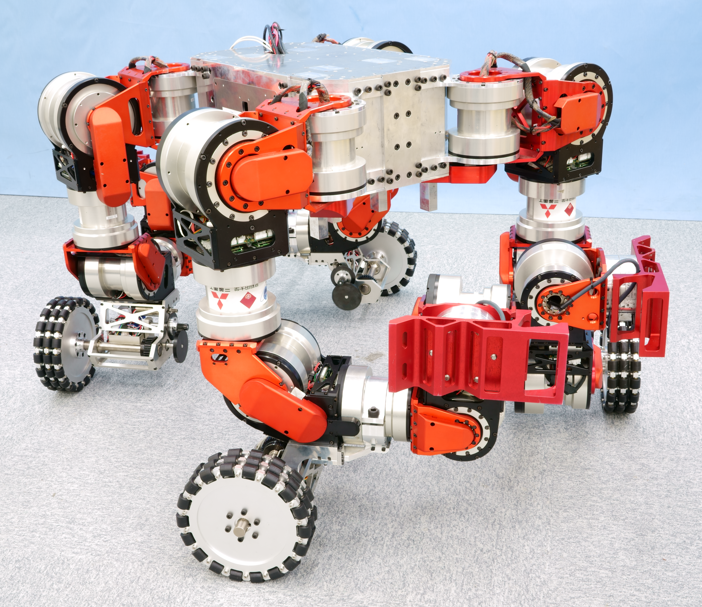
\includegraphics[width=0.3\textwidth]{Images/img_ch1/WAREC1_omniwheel.png}} \\
    \subfloat[WAREC-1R adaptable multimodal locomotion.\label{fig:WAREC_multimodal}]{
    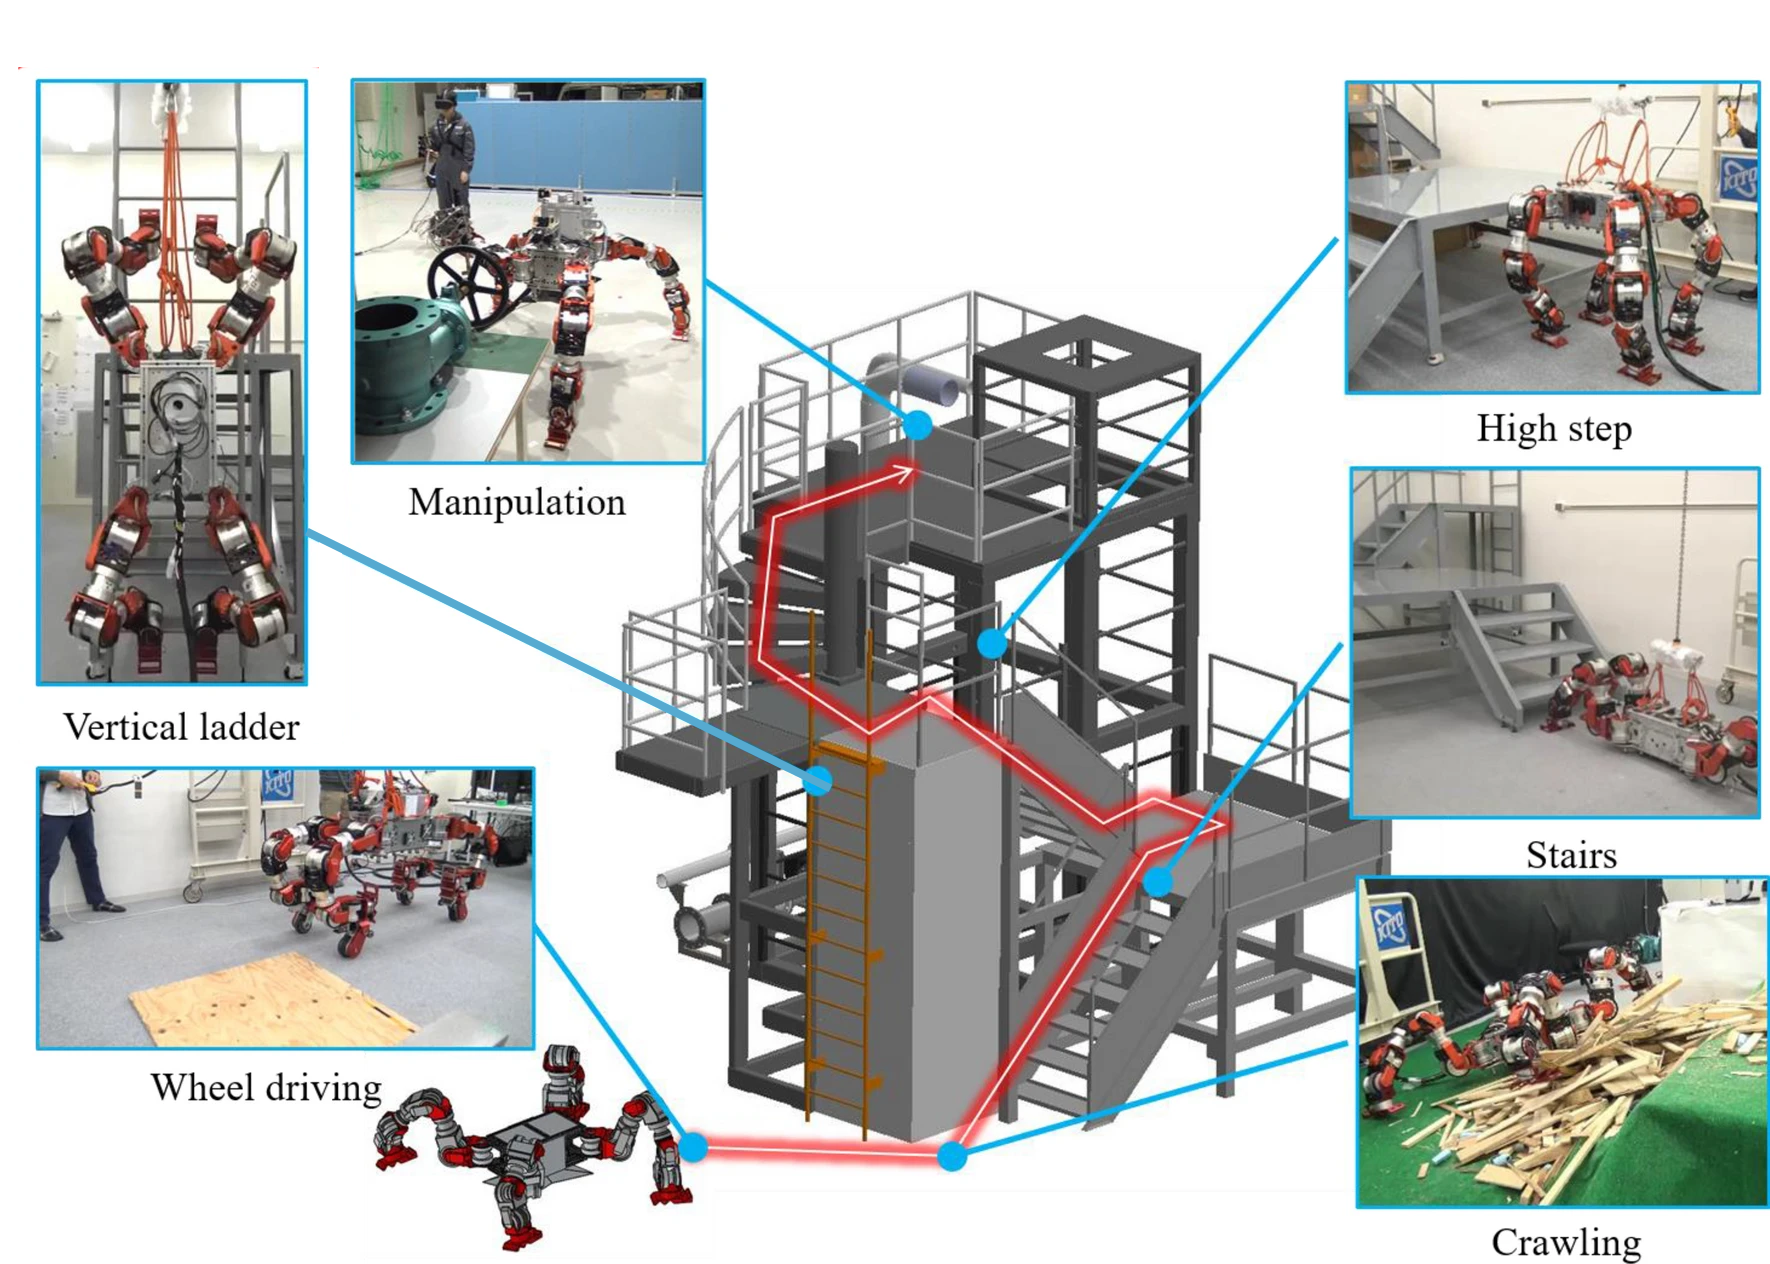
\includegraphics[width=0.9\textwidth]{Images/img_ch1/WAREC1_multimodal.png}}
    \caption[WAREC1, Disaster Response Robot for Extreme Environment]{WAREC1, Disaster Response Robot for Extreme Environment\cite{WAREC_Site}}
    \label{fig:WAREC1}
\end{figure}

The capabilities of WAREC-1(R) outperform other robots in disaster site adaptability, but in non-urbanized outdoor environments   (as the one addressed here) its ladder-climbing capabilities won't be useful, and its weight of 155 kg\cite{WAREC1} can be problematic.  

This section presents an overview of the most advanced robotic systems for unstructured environments, focusing on task capabilities for different terrain conditions. The examples highlight the relevance of the tools that interact with the environment to generate motion or other functions, for this reason, the end effector choice is as important as the robotic structure design. 



\section{Research Motivation and Objectives}
\label{sec:objectives}

In the environment addressed in this thesis, the best-suited robotic system needs climbing, driving, walking, and additional manipulation abilities to complete a full exploration and sampling mission, with the possibility of moving obstacles and freeing space for a safe and rescue operation. 
From these task requirements comes a transformable module developed at the Space Robotics Lab (SRL)\cite{SRL}, an innovative research laboratory of Tohoku University, led by Yoshida Kazuya, where the initial research activity of this thesis has been conducted.
GRIEEL\cite{GRIEELUdaThesis}\cite{GrieelUda}is this transformable Gripper-Wheel module designed and developed by M.Uda, K.Naoki \textit{et all}, members of the Rover Team at the SRL.
This module was created as an adaptable mechanism for any multilimbed robot, and in this research, it is deployed with LIMBERO, a multilimed climbing robot (developed by the Limb Team of the SRL). 

Manipulators and wheeled mobile robots are well-established systems in literature, and also walking machines to some extent. multimodal locomotion and multifunctional robots instead are a recent research trend, without a unique approach to solve the fundamental robotics' problems of modeling, planning, and control\cite{Siciliano}.

The multilimbed multimodal robotic system addressed in this research is in the early stage of development, and setting up the control system, software architecture, planning procedures, and simulation environments is fundamental to ensure smooth and efficient operation in its wheel and gripper mode. When deployed in an unstructured environment \cite{UnstructuredHOW}, reliability is a key requirement, especially for space exploration, where system retrieval is not possible, and failure is not admissible. Furthermore, in safety and rescue missions, completing the task quickly is an additional requirement, that has to be considered in the planning process.

In this work, different problems of modeling, control, and planning have been addressed, such as the design of stable high-level algorithms for the robot mode transformation, the definition of novel performance criteria to evaluate its dexterity, the setup of the simulator for preliminary testing, and the design of the control software architecture to coordinate the motion of the additional transformable model with the limb.
Considering everything above, the final objective is to enable the reliable and efficient autonomous execution of complex missions in unstructured environments, exploiting the multiple locomotion capabilities of this cutting-edge robotic system.  

 
\section{Research Workflow}
\label{sec:approach}

Now the workflow of this thesis is presented, to clarify its “nonlinear” approach towards the objectives defined in the previous section.

As mentioned, this work began at the Space Robotics Lab (Tohoku Univeristy, Japan), to design and implement the control system for the transformable module presented in the previous section, and integrate it with LIMBERO. As a researcher of the SRL, the following activities have been conducted: 
\begin{itemize}
  \setlength\itemsep{-0.7em} 
    \item Implement the software architecture. 
    \item Set up a simulation environment.
    \item Define a reliable locomotion transition algorithm.
    \item Design and Tune the motion control system. 
    \item Conduct experiments on the real system.
\end{itemize}

From the lessons learned from the experiments and the limbed robot state-of-the-art, additional research has been conducted at Politecnico di Milano:
\begin{itemize}
  \setlength\itemsep{-0.7em} 
    \item Set up a new simulator with advanced features, due to inaccessible hardware.  
    \item Redesign of the low-level controller. 
    \item Take a model-based tuning approach for the motion controller.
    \item Define novel performance index to evaluate multilimb robots' dexterity.
    \item Test the transition algorithm on the new simulator.
    \item Evaluate the motion performance based on the new criterion.
    \item Test additional motion task on the simulation environment.
\end{itemize}





\section{Thesis Organization}
\label{sec:organization}


Following this introductory chapter, this thesis is organized into eight chapters, which can be subdivided into five macro arguments: 
\begin{itemize}

    \item \textbf{Theoretical background}\\
    Multipurpose limbed robots are recent research topics, and for this reason, \textbf{Chapters \ref{ch:chapter_two}} and \textbf{\ref{ch:chapter_three}} analyze in detail the possible approaches to analyze these complex systems.  
    Multi-limed robot theory is discussed in \textbf{Chapter \ref{ch:chapter_two}} from a modeling and control point of view, and in \textbf{Chapter \ref{ch:chapter_three}} with a focus on stability and performances.  
    
    \item \textbf{Algorithm definition }\\
    The algorithm implemented for a reliable locomotion transition is explained in \textbf{Chapter \ref{ch:chapter_five}}, based on legged robots' stability. The performance of the designed procedure is analyzed in view of a novel mobility theory, and then the advantages, limitations, and possible extensions are discussed.
    The new mobility theory is introduced in  
    \textbf{Chapter  (\ref{sec:multi_limb_coopmanipulators}}, demonstrating its validity with a bio-inspired example. 
    
    \item \textbf{System description and setup}\\
    The robotic system used, and the preparation and approach of the experiments are accounted for in \textbf{Chapters \ref{ch:chapter_four}}, \textbf{\ref{ch:chapter_six}}, and \textbf{\ref{ch:chapter_seven}}.
    \textbf{Chapter \ref{ch:chapter_four}} presents the hardware and software of LIMBERO-GRIEEL, the multimodal robot used in this research.  In \textbf{Chapters \ref{ch:chapter_six}} and \textbf{\ref{ch:chapter_seven}} respectively, the control tuning and the experimental setup are discussed. In the latter, some limitations of the robotic system are introduced, as part of the experimental procedure description. 

    \item \textbf{Experiments and results}\\
    Final results and limitations on motion control and transformation capability  are discussed in \textbf{Chapter \ref{ch:chapter_eigth}}, both in simulations and with the real robot results. 

    \item \textbf{Conclusions}\\
    Achievements, research contributions, and potential future works are summarized in \textbf{Chapter \ref{ch:chapter_nine}}.
    
    \vspace{1.0cm}
    
    \begin{tcolorbox}[
      colback=bluepoli!20,
      colframe=bluepoli!40, 
      title=Additional Resources,
      sharp corners=south,
      fonttitle=\bfseries,
      coltitle=bluepoli!90!black,
    ]
    As supplementary resources, the hardware experiments and simulations have been documented in a set of videos on \href{https://youtube.com/playlist?list=PLFgoOtxCJKTPv_dibdvSUT_YPGDJBc_5C&si=bgCxZ_qWpax2N8Xt}{YouTube}.
    Furthermore, the MATLAB code used for limbed robot kinematic, dexterity analysis, and algorithm evaluation is on \href{https://github.com/AlePuglisi/limbed-robot-control}{GitHub}.
    \end{tcolorbox}
\end{itemize}






\clearpage
\thispagestyle{empty} % This removes the header/footer but keeps the numbering
\vspace*{\fill} % Pushes everything to the bottom
\newpage

\BlankPageTLGWzero
\chapter{Modeling and Control of Limbed Robots}
\label{ch:chapter_two}%
% The \label{...}% enables the removal of the small indentation that is generated, always leave the % symbol.

The former chapter describes common locomotion systems used for field robots, including new hybrid trends. In addition, the objectives of this research have been introduced, highlighting the importance of limbed locomotion for the system under analysis.
This chapter introduces the main theory behind limbed robot modeling and control, which are fundamental concepts for motion control and performance analysis. 

First, the difference between limbed and legged robots is formally explained.
Once this difference is clear, the kinematic model is introduced, describing forward, inverse, and differential kinematics, and why they are important for any motion task. 
Then, the fundamental equations of the dynamic model are presented, along with a simpler approach to describing them. 
Finally, a common control architecture is described, with an overview of classical and novel controller algorithms.
Those concepts are described for legged robots and manipulators, which are the basics for modeling and controlling limbed robots.  

The tools to describe and analyze performance are presented in chapter \ref{ch:chapter_three}.


\section{Limbed vs Legged Robot}
\label{sec:limbvsleg}

In anatomy, it is clear the difference between leg, arm, and limb, this difference can be defined in the same way in robotics.
"Limb" encompasses both leg and arm, the former has locomotion as a main function, and the latter ensures object manipulation and complex interactions with the environment. 

Theory on manipulators (robotic arms) dates back to the 50s, with the first example Unimate \cite{unimate}. In the next years, also legged robots were coming, with pioners McGhee and Frank \cite{McGhee}. 
The first definitions of limb mechanism in robotics can be found in Koyachi's works. \cite{Koyachi}\cite{Koyachi2}\cite{Koyachi3}.\newline

First, an important classification has to be done.
Robots can be classified as those with a fixed base, \textbf{robot manipulators}, and those with a mobile base, \textbf{mobile robots}\cite{Siciliano}
To introduce legged robots, a definition of manipulator and legged robot is needed.
In the 80s, the Robotics Institute of America (RIA) \cite{Siciliano}\cite{Robotics1} defined manipulators as "robot": 
\begin{definition}\label{def:manipulator}
A \textbf{robot} is a reprogrammable multifunctional \textbf{manipulator} designed to move material, parts, tools, or specialized devices through variable programmed motions for the performance of a variety of tasks.
\end{definition}

Whenever the base can perform some motion, it is considered a \textbf{mobile manipulator} (see Fig.\ref{fig:Manipulators}), entering the class of \textbf{mobile robots}. 

\begin{figure}[H]
    \centering
    \subfloat[CHIMERA Mobile manipulator.\label{fig:MobileManipulator}]{
        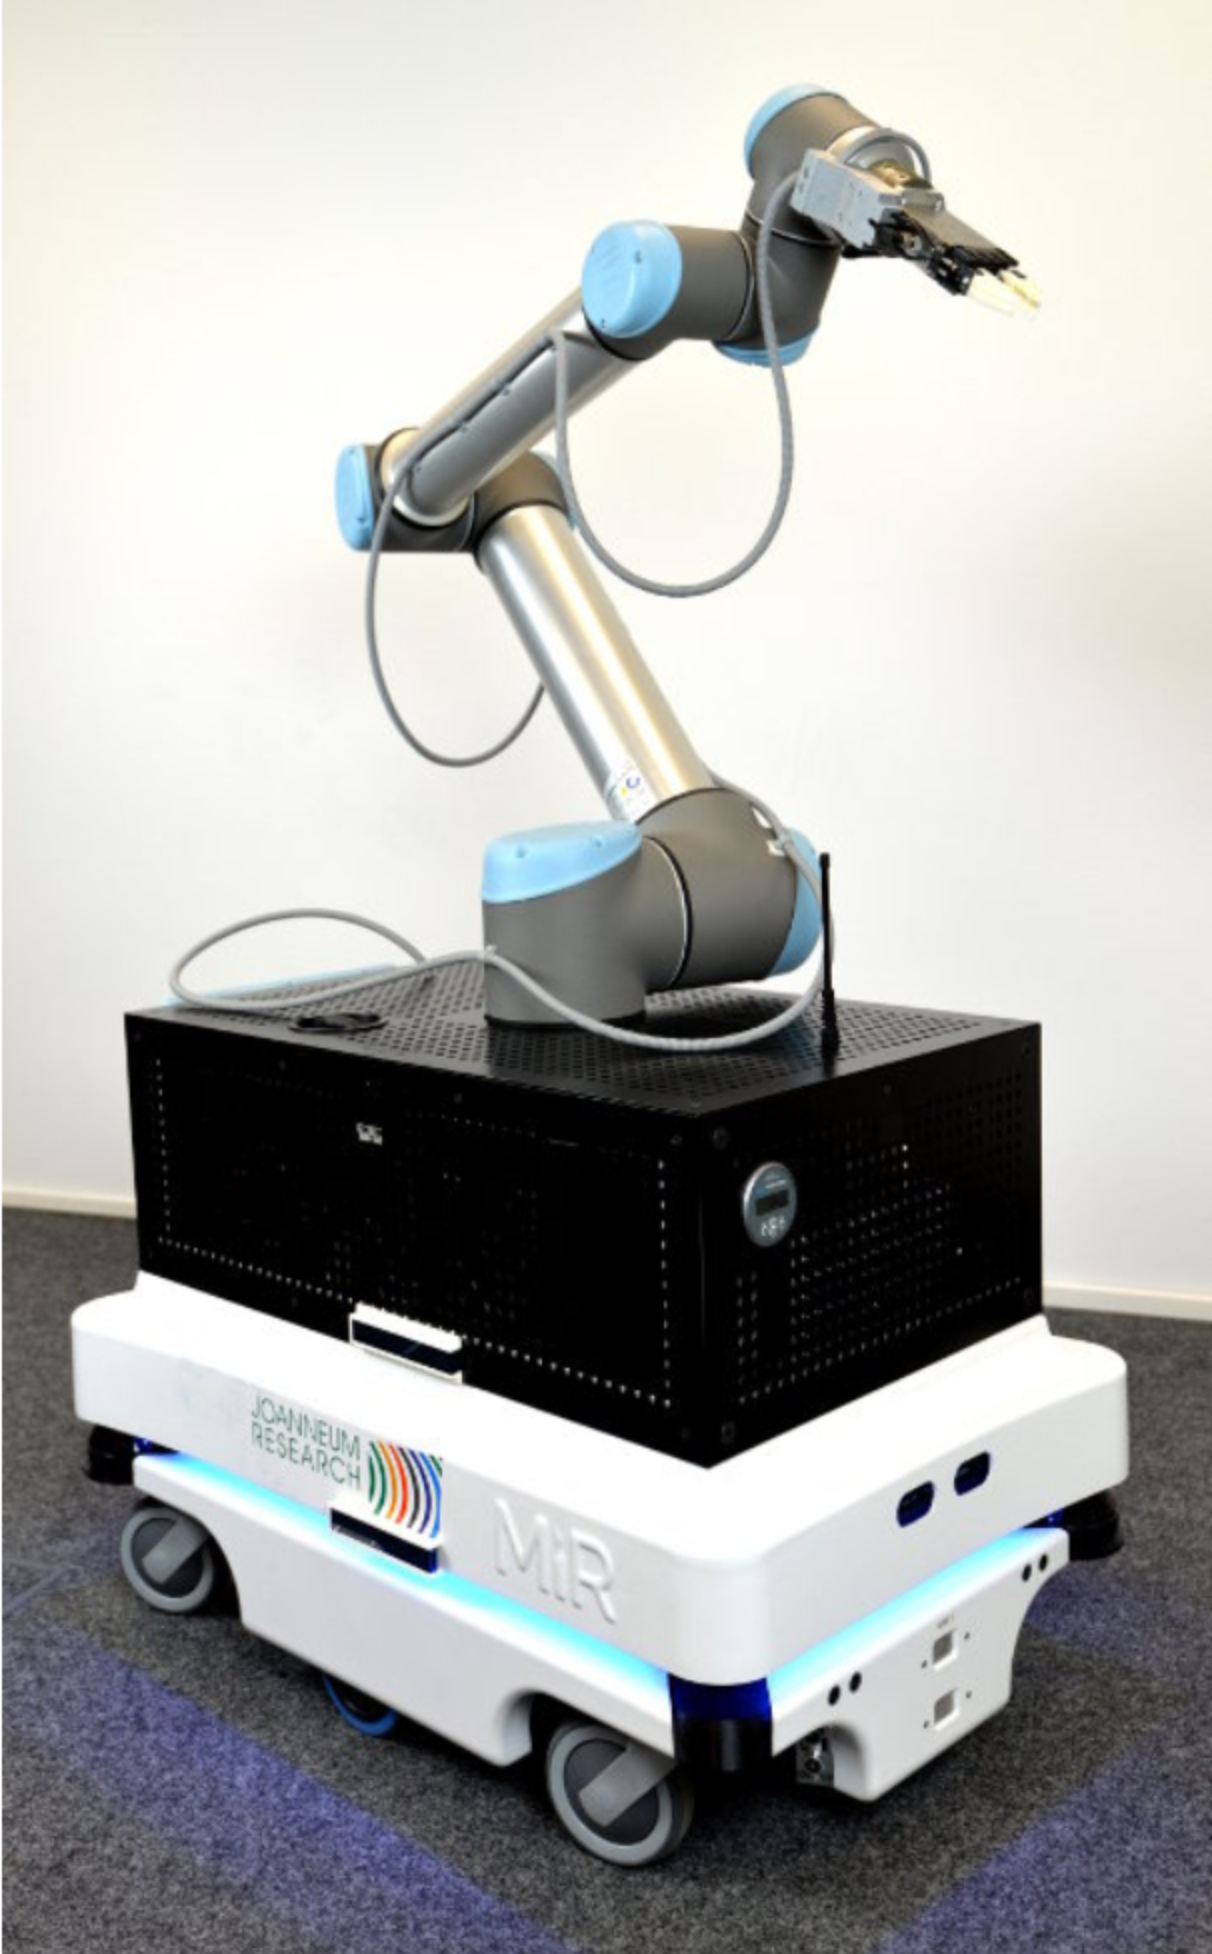
\includegraphics[scale=0.13]{Images/img_ch2/MobileManipulator.png}
    }
    \subfloat[KUKA-DLR manipulator.\label{fig:Manipulator}]{
        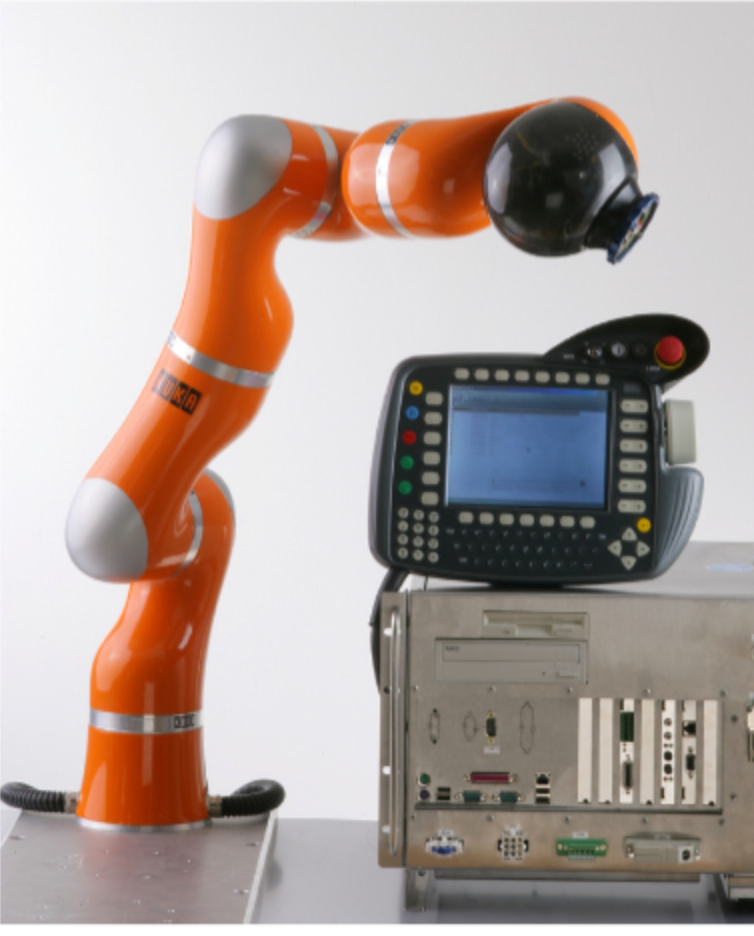
\includegraphics[scale=0.25]{Images/img_ch2/KUKA.png}
    }
    \caption[Examples of manipulators fixed and not.]{\cite{MOBILEMANIPULATOR}Mobile manipulator and \cite{KUKA}robotic arm}
    \label{fig:Manipulators}
\end{figure}

Raibert\cite{Raibert} and Todd\cite{Todd} give an extensive analysis of walking machines, while a clear definition of a legged robot can be found in \cite{Siciliano} or \cite{Legged}:

\begin{definition}\label{def:leggedSiciliano}
\cite{Siciliano}\textbf{Legged Robots} are made of multiple rigid bodies, interconnected by joints. Some of these bodies
form lower limbs, whose extremities (feet) periodically come in contact with the ground to realize locomotion
\end{definition}

\begin{definition}\label{def:legged}
\cite{Legged}\textbf{Legged Robots} use legs to move from one place to another. Legs provide an active suspension, so the motion of the main body of the robot can be largely decoupled from the terrain profile. With each step, a leg is temporarily
lifted off the ground, so that discontinuous terrain can be overcome as well, allowing locomotion in places out of reach otherwise.
\end{definition}

In the same article\cite{Legged}, legs in robotics are defined as:
\begin{definition}\label{def:leg}
\textbf{Legs} are usually articulated rigid bodies, assumed to contact the environment only with their end effector(EE). In most cases, this contact is unilateral,
meaning that the robot can push but not pull on contact surfaces
\end{definition}

In general, the design of legs is done to achieve walking locomotion (such as the quadrupeds in Fig.\ref{fig:WalkingRobots}). Using proper mechanical structures or innovative solutions\cite{climbing1}\cite{LEMUR3}\cite{SCARE_gripper}, also locomotion in walls and ceilings is possible, obtaining \textbf{climbing robots} (as the one in Fig.\ref{fig:LEMUR3}).

Finally, from Koyachi's works on multi-limbed robots, an explicit definition of limbed mechanism is given \cite{Koyachi}\cite{Koyachi2}\cite{Koyachi3}:

\begin{figure}[H]
    \centering
    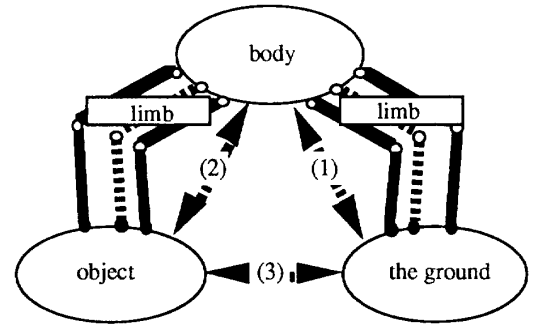
\includegraphics[width=0.5\textwidth]{Images/img_ch2/limb-mechanism.png}
    \caption{Scheme of Limb mechanism.\cite{Koyachi}}
    \label{fig:limb-mechanism}
\end{figure}

\begin{definition}\label{def:limb_mechanism1}
In robotics, a \textbf{Limb mechanism} is a link that connects the robot body with the environment. The objective with limb mechanism is to obtain the following motions (as in Fig.\ref{fig:limb-mechanism}) by moving each limb appropriately:
  \begin{itemize}
      \item (1) Relative motion between body and ground that
        causes locomotion of the robot.
      \item (2) Relative action between an object and a body that will
be used for handling and machining a small object.
      \item (3) Relative action between an object and base that will be
used for transferring and handling of an object, machining
of a large object.
  \end{itemize}
\end{definition}

From another publication of the same author\cite{Koyachi3}:  
\begin{definition}\label{def:limb_mechanism2}
In robotics, a \textbf{Limb mechanism} is a linkage integrating both locomotion and manipulation functions.
Ensuring the following features: 
\begin{itemize}
\item There is no clear boundary between walking and working spaces, and total efficiency increases because limbs can be used for walking or working according to the situation
\item Force generated by the hand increases and working space
is expanded because limbs can be coordinated and support
limbs can move the body
\item This mechanism can be compact and light because two
functions are integrated into one linkage.
\end{itemize}
\end{definition}
The working space, also called \textbf{workspace}, comes from manipulator theory, and it is defined as \cite{Siciliano}:
\begin{definition}\label{def:workspace}
The \textbf{workspace} is the region described by the origin of the end-effector frame when all the manipulator joints execute all possible motions.
\end{definition}

A formal definition of multi-limb robot cannot be found in literature, but an intuitive one can be deducted from the ones above: 

\begin{definition}\label{def:multilimb_robot}
A \textbf{multi-limb robot} is composed of a body and multiple limb mechanisms. Limb-end integrates both locomotion and manipulation through suction cups, magnets, adhesive materials, or miniature spine arrays \cite{Legged}\cite{Hirose1991}\cite{HorizontaltoVertical}\cite{passiveSpineTohoku}. In some cases, even \textbf{limb/leg}-wheeled \cite{AnymalDocThesis}\cite{WheelLegged}\cite{MAMMOTH}\cite{RollerWalker}\cite{HopperLegWheel} or multimodal mechanisms can be integrated\cite{GrieelUda}\cite{Armadillo}. If a transformable multimodal mechanism is used as limb-end, the robot can be defined \textbf{multi-modal}.
\end{definition}
SCAR-E in Fig.\ref{fig:SCARE} is a good example of a multi-limb robot, with its gripper(Fig.\ref{fig:SCARE_Gripper}) designed for climbing, manipulating, and walking.

To avoid any confusion, a final comment on robotic system classification has to be done, regarding the class of \textbf{Humanoid robots}\cite{HumanoidRobot}. These robots have a human-like physical appearance, with both manipulator and walking abilities, but the mechanical structures (arms and legs) used to achieve those tasks are different. Multi-limbed robots instead perform multiple tasks with the same limb structure. 

\begin{figure}[H]
    \centering
    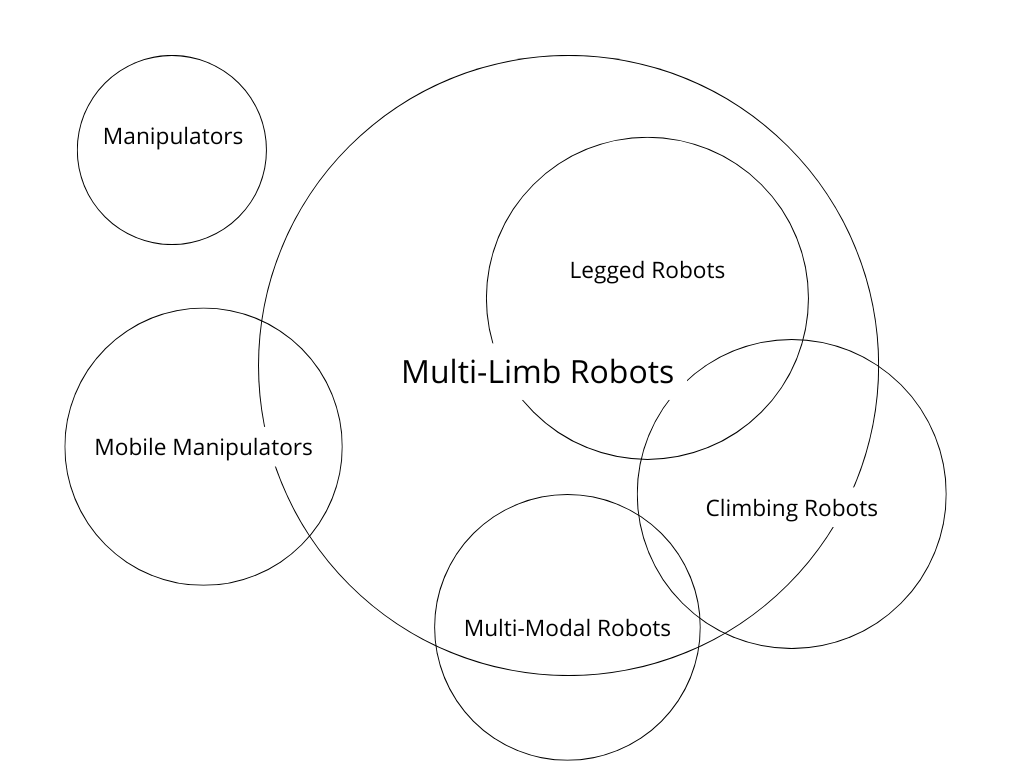
\includegraphics[width=0.8\textwidth]{Images/img_ch2/RobotClassificationVENN.png}
    \caption{Diagram of some robot classes}
    \label{fig:robotclasses}
\end{figure}

It is hard to identify a clear boundary among some of these classes of robots. Fig.\ref{fig:robotclasses} provides a diagram to summarize the concepts described in this section. 
This broad but mild classification highlights the reason why modeling and controlling limbed robots is not a simple task. 
A unique established theory doesn't exist. In the next chapters, first, state-of-the-art models of robot manipulators and legged robots are formalized, and then, some insights on possible solutions for limbed robots are given.

\section{Kinematic Model}
\label{sec:kinematic}

In mechanics, kinematics studies motion without considering its causes. When flexibility and softness are negligible in the system under analysis, rigid body theory is used.   

The rigid parts of the robot, also called links, are connected by joints, usually prismatic or revolute \cite{Siciliano}. The mobility of any robot is ensured by those joints, providing a single degree of freedom (DOF) each. 
An important concept when considering multi-body mechanics is the nature of the \textbf{kinematic chain}\cite{Siciliano}\cite{RoboticMechanics}. We classify it as: 
\begin{itemize}
\item \textbf{open kinematic chain} when only one sequence of links connects the mechanical chain's two ends (Fig.\ref{fig:openkin}). For example robot manipulators, but even dual-arm robots.
\item \textbf{closed kinematic chain} when the sequence
of links forms a loop(Fig.\ref{fig:closedkin}).
\end{itemize}. As a Parallelogram mechanism (used in construction vehicles), or legged robots, considering the "connection" between feet tip through a common ground \cite{RoboticMechanics}\cite{QuadrupedLocomotion}. 

\begin{figure}[H]
    \centering
    \subfloat[Open chain.\label{fig:openkin}]{
        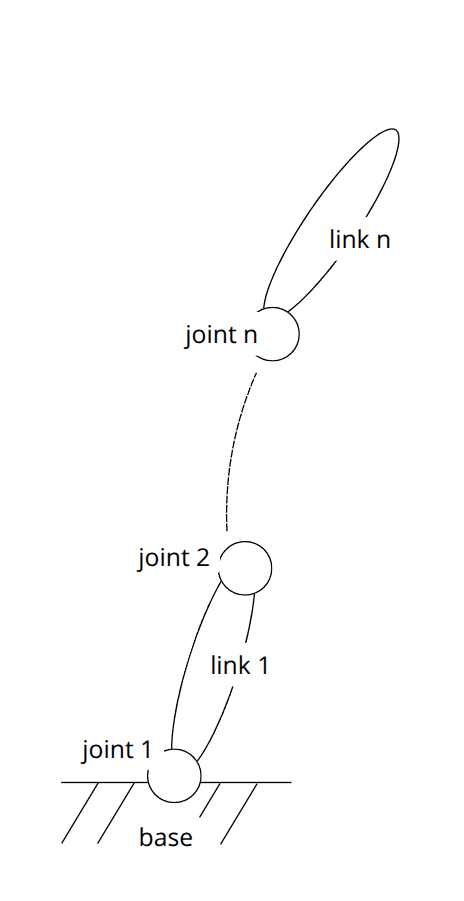
\includegraphics[scale=0.3]{Images/img_ch2/OpenKinChain.png}
    }
    \quad
    \subfloat[Closed chain.\label{fig:closedkin}]{
        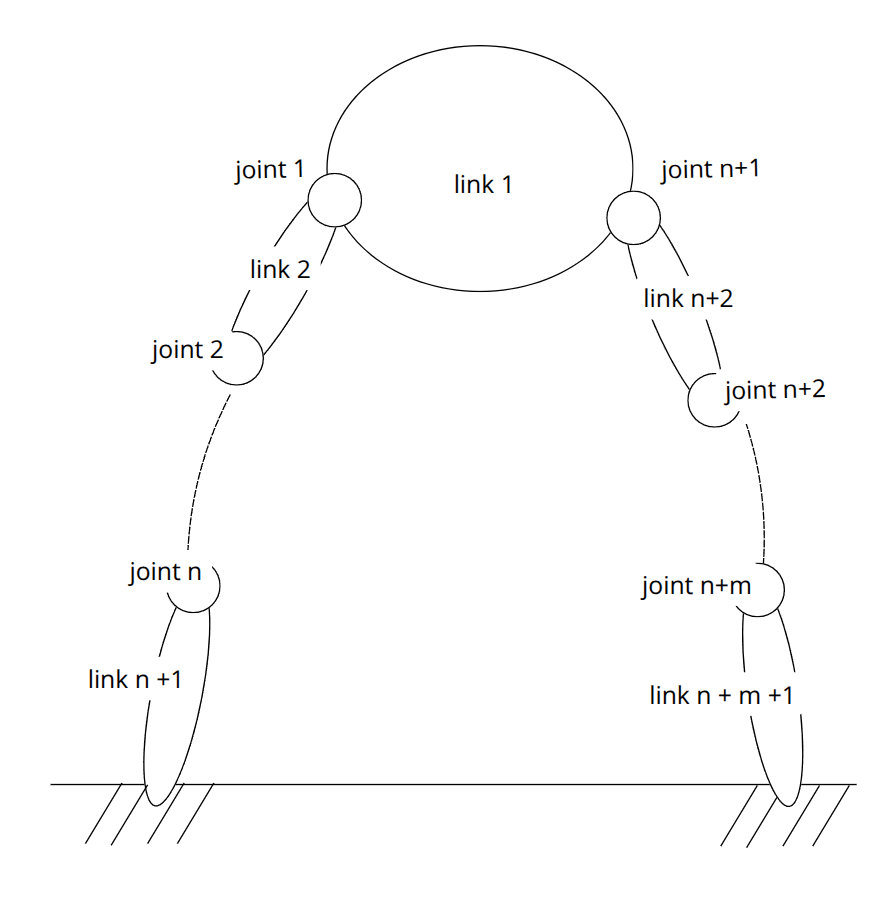
\includegraphics[scale=0.3]{Images/img_ch2/ClosedKinChain.png}
    }
    \caption[Scheme of possible kinematic chains]{Simple representation of open/closed kinematic chains.}
    \label{fig:quadtree2}
\end{figure}


In robotics, three main problems are considered: \textbf{forward}(FK), \textbf{inverse}(IK), and \textbf{differential kinematics} (DK). These are formally defined and solved for manipulators, legged, and multi-limb robots. 

\subsection{Forward Kinematic}
\label{sec:forward}
The role of FK is to derive the relationship between joint variables and the pose of a final link frame\cite{CorkeMATLAB}\cite{Siciliano}. 
The "final link" depends on the type of robot. 
For a manipulator, it is the end effector, which is the last element of the open chain, usually carrying a tool. 
In legged and multi-limb robots, the pose of all legs/limbs tips is important. 

Independently of the structure under analysis, the foundation of kinematics is the relationship between link frames. Each link is identified by an attached reference frame, and its pose is defined as the position and orientation of that frame \cite{Siciliano}\cite{RoboticMechanics}\cite{CorkeMATLAB}.
The choice of each link frame is not unique, the \textbf{Denavit-Hartenberg} (DH) convention \cite{DenavitHartenberg} provides a standard way to define it.

Collecting all variables of the n joints in a vector $\mathbf{q} \in \mathbb{R}^n$ (time dependency is omitted), the final result of FK is a homogenous 4x4 transformation matrix $\mathbf{T^0_f(\mathbf{q})}$, "0" identify the inertia frame, "f" the final frame in consideration. 
This matrix contains information about the position and orientation: 
\begin{equation}
\label{eq:homogeneus}
    \mathbf{T^0_f(\mathbf{q})} =
        \begin{bmatrix}
        \mathbf{R^0_f(\mathbf{q})} & \mathbf{^0p_f(\mathbf{q})} \\
        \mathbf{0}^{\top} & 1
        \end{bmatrix}
\end{equation}

Here, the dependency on joint configuration \textbf{q} is explicit, to clarify how FK is a function of joint configuration, for notation conciseness, sometimes it is omitted.
Furthermore, "0" is omitted in some cases, considering the inertial frame granted, 
$\mathbf{R^0_f} = \mathbf{R_f}$, $\mathbf{^0p_f} = \mathbf{p_f}$, and so on.
$\mathbf{T^0_f}$ is a powerful mathematical tool that not only contains information about the pose but also a matrix transformation to change the reference frame. If we consider the homogeneous coordinates ($\tilde{p} = \begin{bmatrix}
    \textbf{p} & 1
\end{bmatrix}^T$) of a generic point A in space, it holds:
\begin{equation}
\label{eq:pointTransform}
    \mathbf{\tilde{^0p_A}} = \mathbf{T^0_f} \cdot \mathbf{\tilde{^fp_A}} 
\end{equation}


Additionally, transformation matrix composition is as easy as a matrix product, and it can be chained.
\begin{equation}
\label{eq:chainTransform}
    \mathbf{T^0_f} = \mathbf{T^0_i} \cdot \mathbf{T^i_j} \cdot ... \cdot \mathbf{T^m_f}
\end{equation}

The drawback of using homogeneous transformation is the redundancy of $\mathbf{R^0_f}$ as orientation description. 
 Minimal or quai-minimal representations such as Euler angles or quaternion are often used \cite{Siciliano}.

In general, a pose in 3D space is described by 6 DOFs, 3 for rotation and 3 for orientation. In some cases, the task of the robotic structure requires less than 6 DOFs, and a task vector $\mathbf{x} \in \mathbb{R}^m$  is defined. The space in which the task is defined is called \textbf{operational/task space} (of dimension m), and it is always possible to derive a non-linear function, relating joint variables (in the so-called \textbf{joint space}) to this task vector: 
\begin{equation}
\label{eq:directKinematic}
    \mathbf{x} = \mathbf{k(q)}
\end{equation}

$\mathbf{x}$ collects position (\textbf{p}) and orientation (\textbf{$\phi$}) as: 
    $\mathbf{x} = \begin{bmatrix}
        \mathbf{p} & \mathbf{\phi}
    \end{bmatrix}^T $

A common minimal representation of orientation is the XYZ Euler angles also called Roll $\vartheta$, Pitch $\varphi$, Yaw $\psi$(RPY) (see Fig.\ref{fig:RPY}):
$\mathbf{\phi} = \begin{bmatrix}
        \vartheta &  \varphi &  \psi
    \end{bmatrix}^T$

\begin{figure}[H]
    \centering
    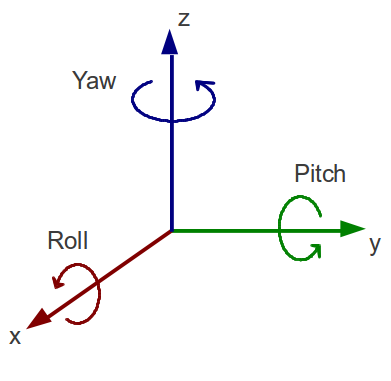
\includegraphics[width=0.3\textwidth]{Images/img_ch2/RPY.png}
    \caption{Roll Pitch Yaw angles}
    \label{fig:RPY}
\end{figure}

The explicit expression of the vectorial function $\mathbf{k(q)} \in \mathbb{R}^m$ is often derived by geometrical analysis of the robotic structure ($\mathbf{T^0_f}$ can also be computed in this way).

\begin{figure}[H]
    \centering
    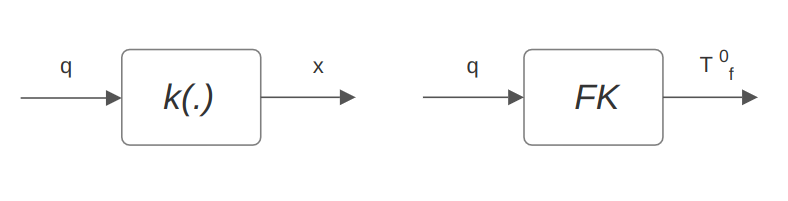
\includegraphics[width=0.8\textwidth]{Images/img_ch2/FKScheme.png}
    \caption{Block scheme of FK problem}
    \label{fig:FKScheme}
\end{figure}

Fig. \ref{fig:FKScheme} summarizes the kinematic problem and its resolution, Solving it is easy for an open kinematic chain robot, problems arise when the system presents closed chains.

The next part of this section presents techniques to solve FK for the robotics structure of interest.

\subsubsection{Manipulators and Single-Leg/Limb}
\label{sec:manipulatorFK}

\begin{figure}[H]
    \centering
    \subfloat[\cite{UR_DH_Parameters}UR DH frames.\label{fig:UR}]{
        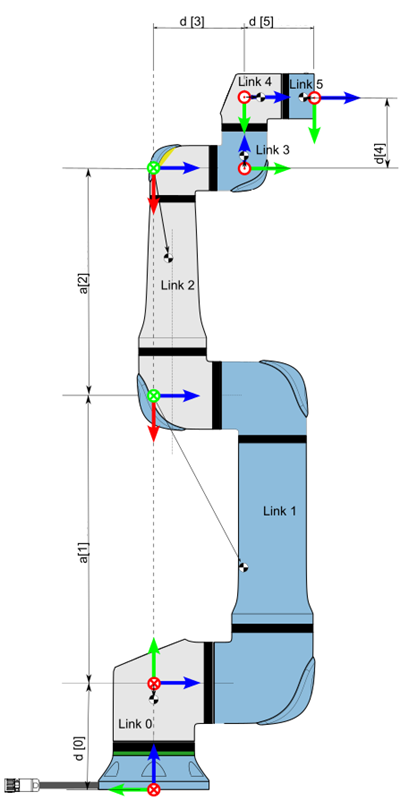
\includegraphics[scale=0.35]{Images/img_ch2/URKinematic.png}
    }
    \subfloat[\cite{Siciliano}Open kinematic chain frames.\label{fig:manipulatorFK}]{
        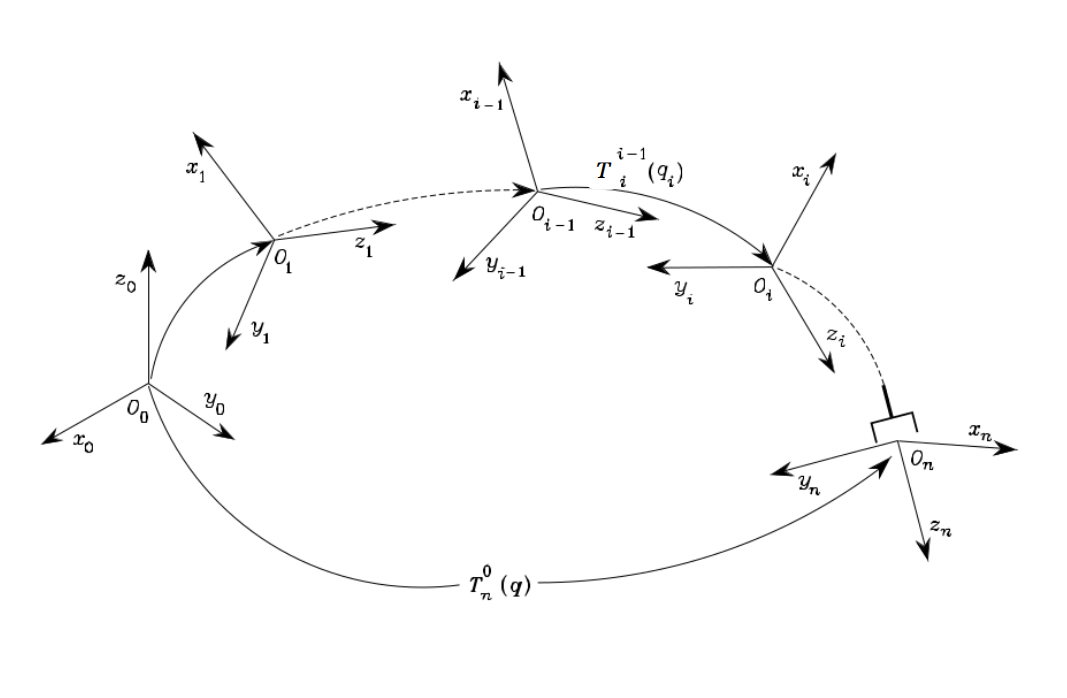
\includegraphics[scale=0.25]{Images/img_ch2/OpenChainKinFK.png}
    }
    \caption[forward kinematic in manipulators]{Example of DH Frames  in UR series manipulator(a), and scheme of open kinematic chain frames(b)}
    \label{fig:FKManipulator}
\end{figure}

In the context of \textbf{Robotic Manipulators}, the final frame (previously called \textbf{f}) is usually the final link frame (where a tool can be attached), defined as frame \textbf{n} (other times as end-effector frame \textbf{e}). 
Considering relation (\ref{eq:chainTransform}), for an open chain of n links, as the one in Fig.\ref{fig:manipulatorFK}, the resolution of FK with \textbf{homogeneous transformations} is straightforward:
\begin{equation}
\label{eq:FKManipulator}
    \mathbf{T^0_n(q)} = \mathbf{T^0_1(q_1)} \cdot \mathbf{T^1_2(q_2)} \dots \cdot \mathbf{T^{i-1}_{i}(q_i)} \dots \cdot \mathbf{T^{n-1}_n(q_n)}
\end{equation}

With $q_{i}$ defining the joint connecting links $i-1$ to $i$, It is straightforward that  $\mathbf{T^{i-1}_{i}(q)} = \mathbf{T^{i-1}_{i}(q_i)} $.

In principle, the choice of each link frame is arbitrary, nevertheless, respecting the DH convention (as in Fig.\ref{fig:UR}) brings some advantages:  
\begin{itemize}
    \item It is a standard convention, which avoids any ambiguity.
    \item $\mathbf{T^{i-1}_{i}(q_i)}$ $\forall i$ can be computed in a standard form from DH Parameters.
\end{itemize}

In simple cases, such as the manipulator in Fig.\ref{fig:ThreeLinkPlanar}, the pose of the final frame can be computed explicitly using \textbf{geometric considerations}. 

\begin{figure}[H]
    \centering
    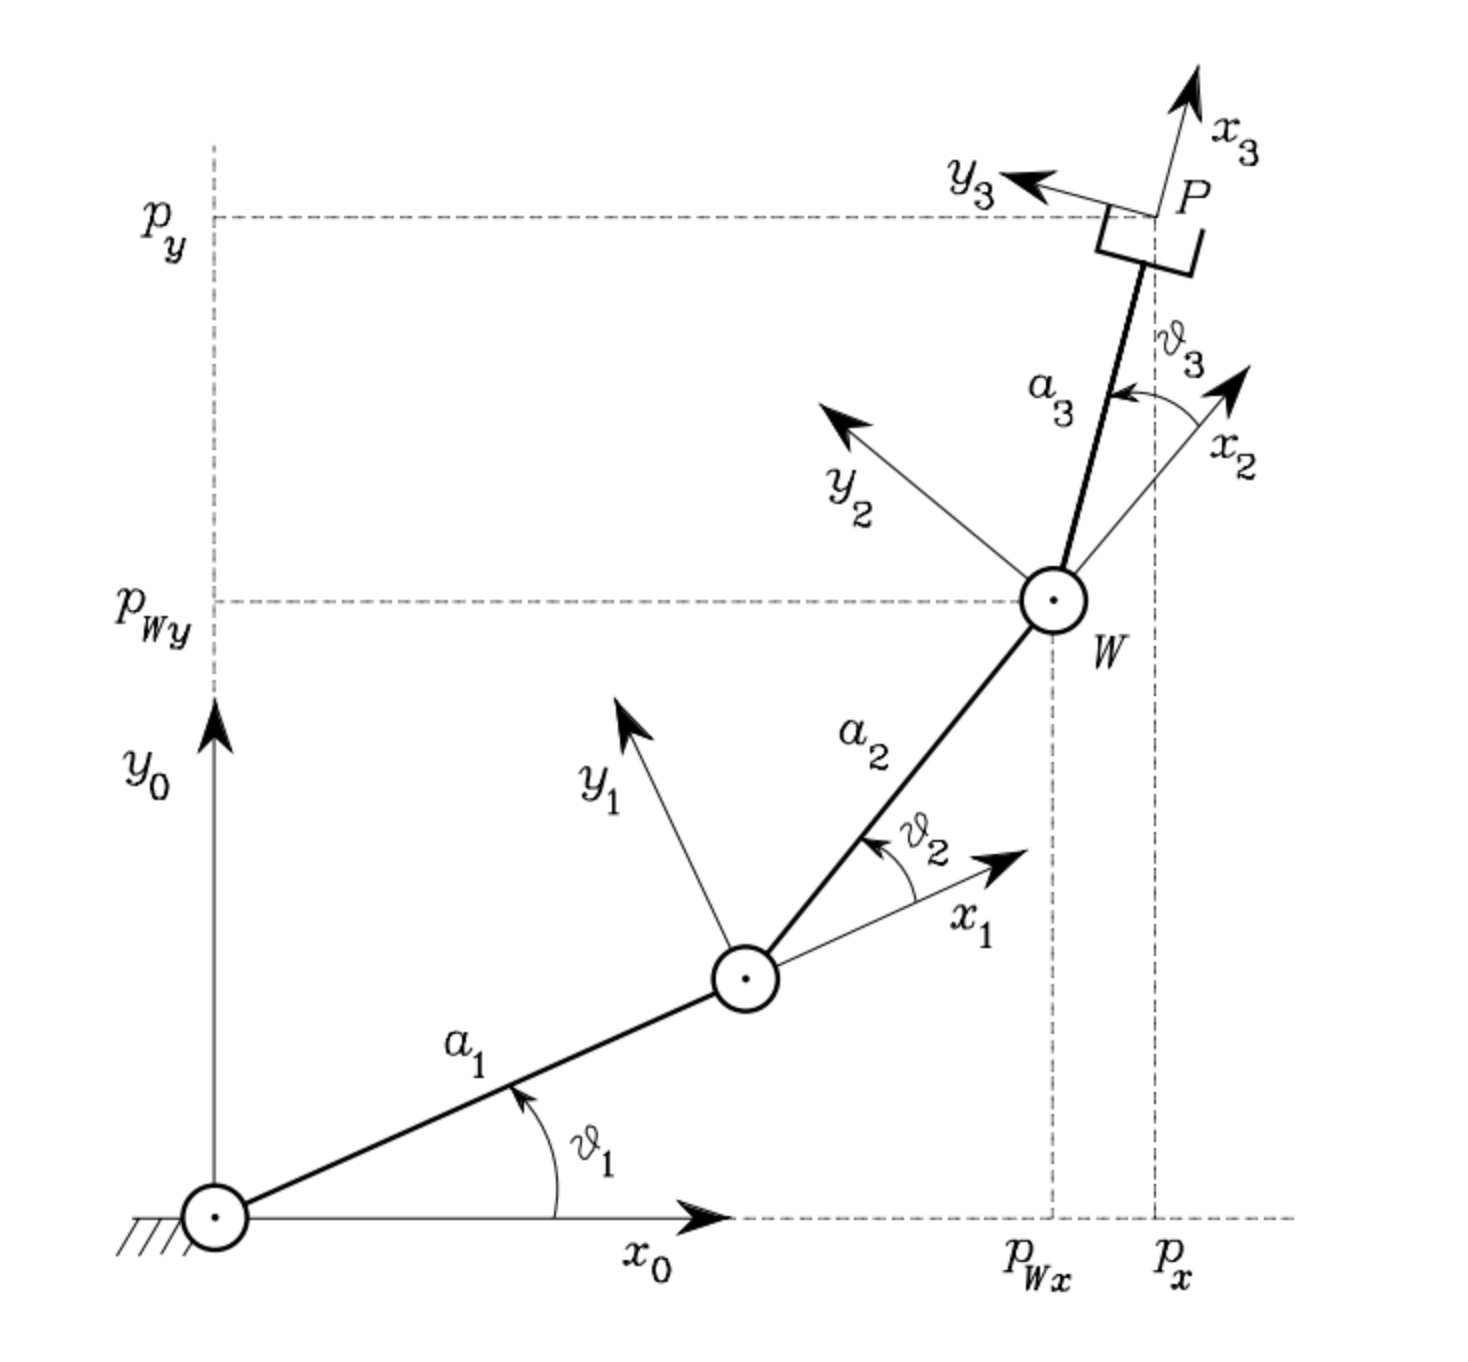
\includegraphics[width=0.6\textwidth]{Images/img_ch2/ThreeLinkPlanarArm.png}
    \caption{\cite{Siciliano}Three-link planar arm}
    \label{fig:ThreeLinkPlanar}
\end{figure}

The Three-link planar arm above provides useful insights into the meaning of \textbf{task space}. 
This mechanical structure allows planar motion in the XY plane. 
with reference to the symbols in the figure, $\mathbf{q} = \begin{bmatrix}
\vartheta_1 & \vartheta_2  & \vartheta_3 \end{bmatrix}^T$, $\mathbf{x} = \begin{bmatrix}
p_x & p_y  & \psi \end{bmatrix}^T$, where $p_x$, $p_y$ represents the EE position, while  $\psi = \vartheta_1 + \vartheta_2  + \vartheta_3 $ the EE orientation (as yaw angle). 
Deriving the expression of $\mathbf{T^{0}_{3}(q)}$ or $\mathbf{k(\cdot)} \in \mathbb{R}^3$ is not relevant here.

To introduce some commonly used reference frames, consider the following example. 
In Fig.\ref{fig:TITAN4Frames} below, the TITAN4 \cite{manipulatorTITAN4} is considered, with a fixed base. The inertial frame is the world frame \textbf{w}, \textbf{b} is a fixed frame attached to the base, frames from \textbf{0} to \textbf{n} identify robot links, and finally \textbf{e} is attached to the EE. 
Homogeneous transformation composition as in \ref{eq:FKManipulator} is used:
\begin{equation}
\label{eq:FKTITAN4}
    \mathbf{T^w_e(q)} = \mathbf{T^w_b} \cdot \mathbf{T^b_0}\cdot \mathbf{T^0_1(q_1)}  \dots \cdot \mathbf{T^{i-1}_{i}(q_i)} \dots \cdot \mathbf{T^{n-1}_n(q_n)}\cdot \mathbf{T^n_e}
\end{equation}
Defining the pose of the EE frame in the world inertial frame. 


\begin{figure}[H]
    \centering
    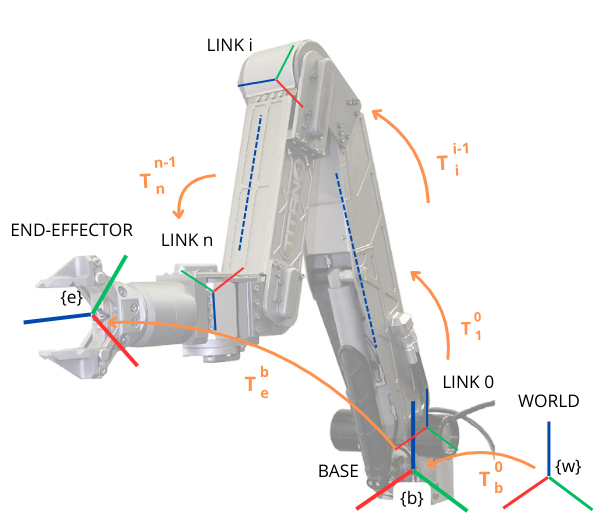
\includegraphics[width=0.7\textwidth]{Images/img_ch2/TITAN4.png}
    \caption{\cite{manipulatorTITAN4}Reference frames of fixed manipulator TITAN4}
    \label{fig:TITAN4Frames}
\end{figure}

These concepts can be extended to any open-chain structure, even to a stand-alone robotic leg/limb (as the ones defined in Def.\ref{def:leg} and  Def.\ref{def:limb_mechanism2}).

For example, the robotic leg in Fig.\ref{fig:KinematicLeg} has been described with the DH convention, to analyze the gait of a large-load-ratio six-legged robot \cite{LegDH}.
Here, the model considers the open kinematic chain from the leg root to the leg tip (as the final frame). 
With reference to Fig.\ref{fig:LegFrames}, denoting the frame attached to the leg root as \textbf{r}, and the one on the leg tip as \textbf{f}, it is possible to derive $\mathbf{T^r_f}$. Then, $\mathbf{T^w_r}$ is needed to obtain position and orientation in the inertial frame. This transformation matrix can be derived as $\mathbf{T^w_r} = \mathbf{T^w_b} \cdot \mathbf{T^b_r} $, where $\mathbf{T^w_b}$ denote the transformation from world inertial frame to the robot base, while $\mathbf{T^b_r}$ from robot base to limb root. It is just a matter of transformation composition. 

So, if the base pose is known ($\mathbf{T^w_b}$), it is possible to track the foot motion when the leg is above the ground. The same holds for any \textbf{limbs}, this modeling approach and classical manipulator FK theory can be used to plan manipulation tasks or limb motion. 

\begin{figure}[H]
    \centering
    \subfloat[Concept of 3 DOF robotic leg for walking.\label{fig:Leg}]{
        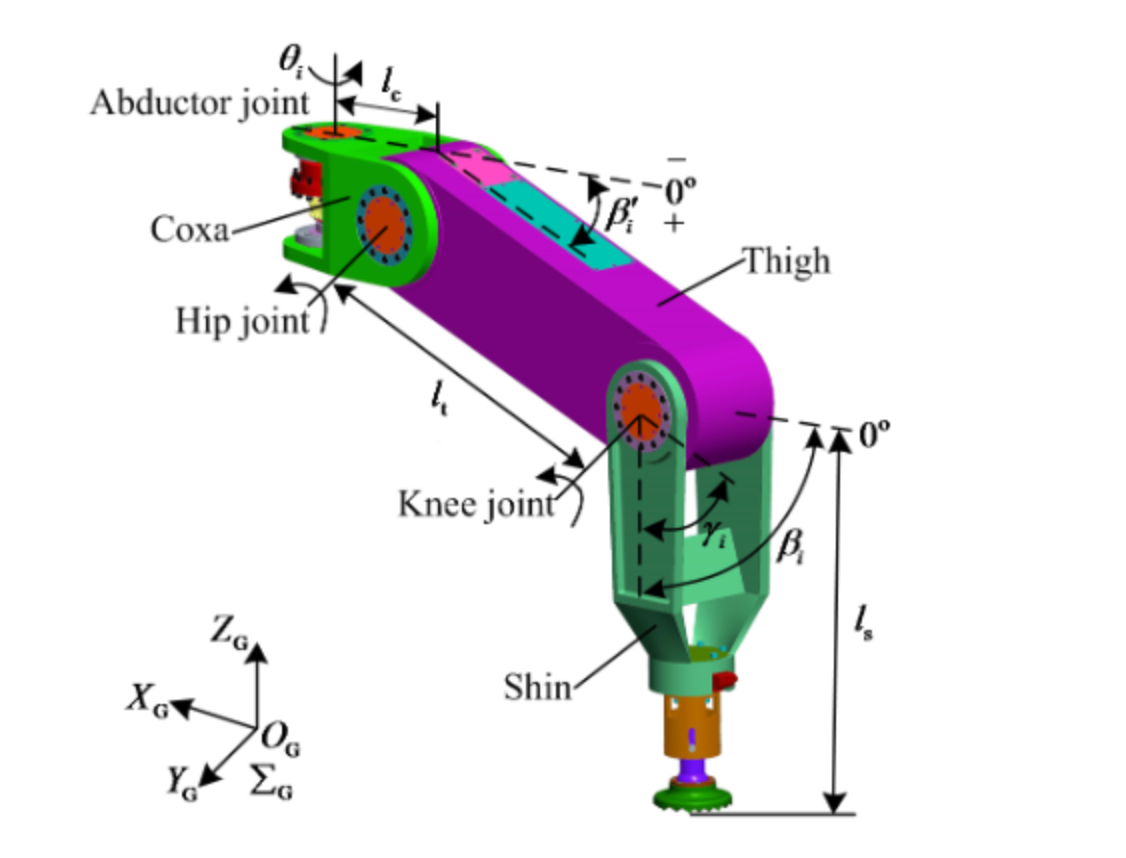
\includegraphics[scale=0.20]{Images/img_ch2/RoboticLeg.png}
    }
    \subfloat[DH frames for the same leg.\label{fig:LegDH}]{
        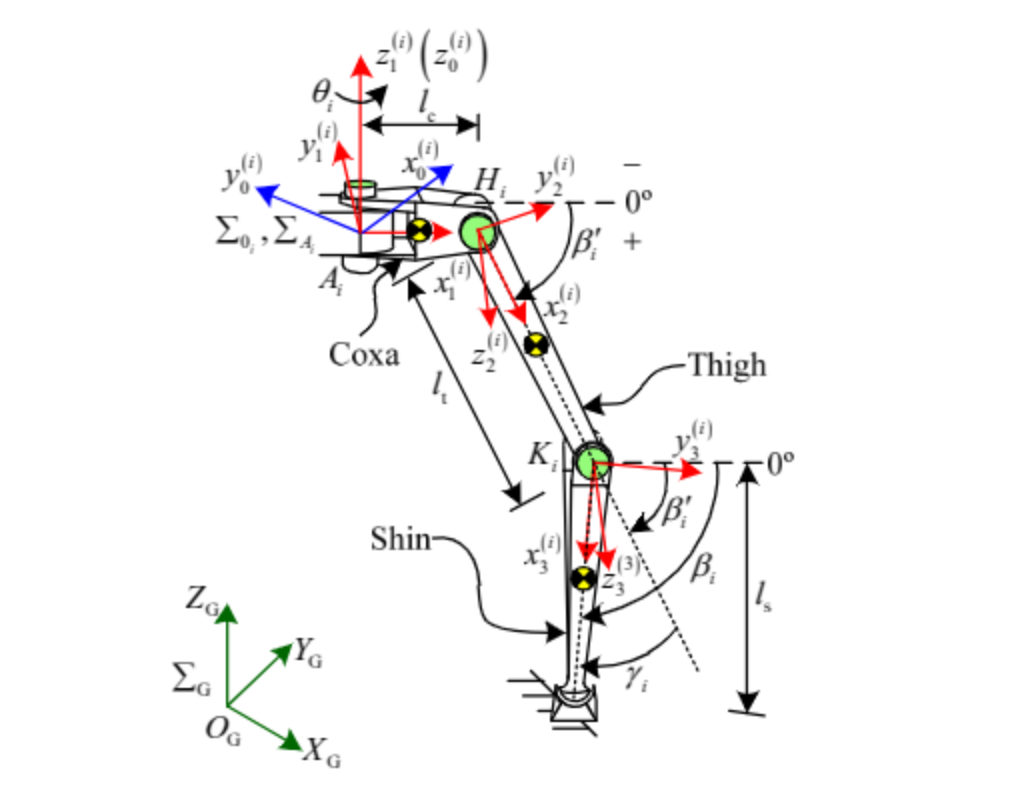
\includegraphics[scale=0.25]{Images/img_ch2/RoboticLegDH.png}
    }
    \caption[Open Kinematic chain Leg DH]{\cite{LegDH} Leg design and DH frames as open kinematic chain}
    \label{fig:KinematicLeg}
\end{figure}

\begin{figure}[H]
    \centering
    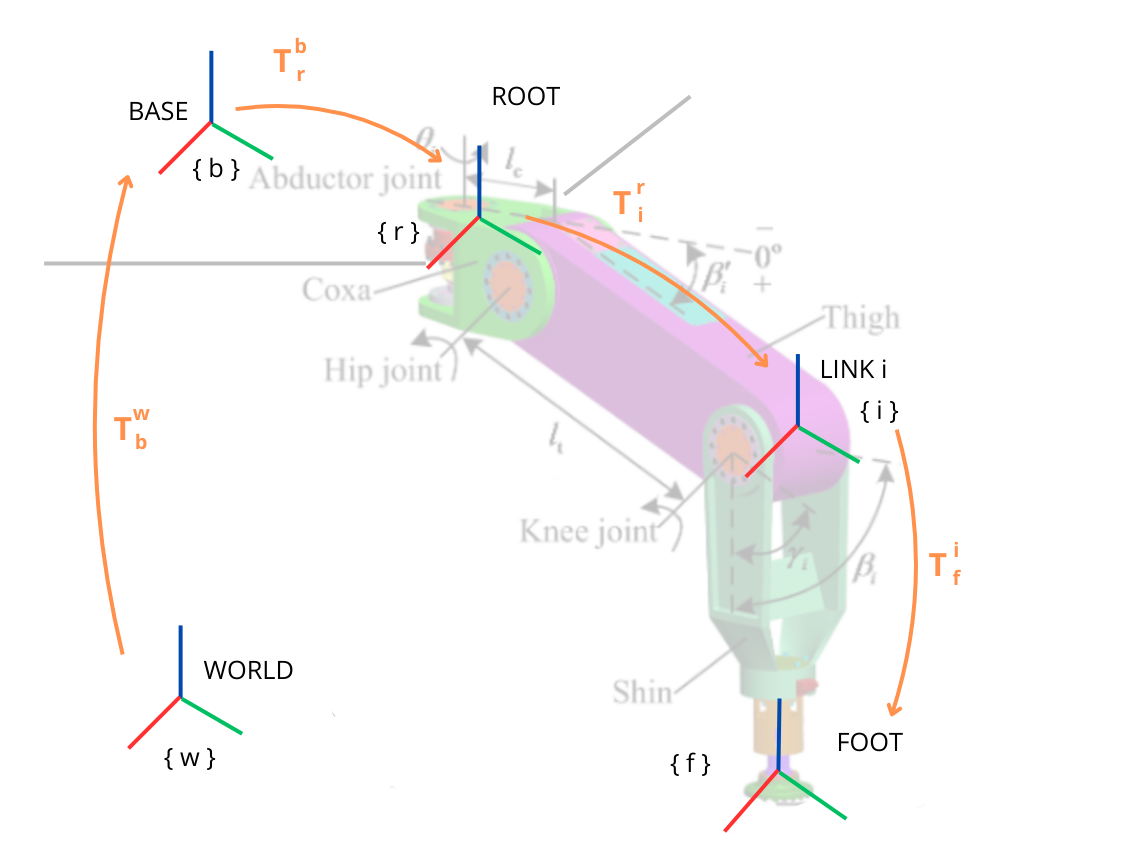
\includegraphics[width=0.7\textwidth]{Images/img_ch2/LIMB_FRAMES.png}
    \caption{Reference frames of single leg}
    \label{fig:LegFrames}
\end{figure}

It is important to notice the difference between the fixed manipulator and leg/limb kinematic. While in the first $\mathbf{T^w_b}$ is fixed and usually known, in the latter, the base is in motion, so $\mathbf{T^w_b}$ changes over time. The same holds when a mobile manipulator kinematic is analyzed. 
In the next section, this difference is further analyzed to define the kinematic of legged robots. 


\subsubsection{Legged Robots, Walking Machines}
\label{sec:leggedFK}

First, some terminology and symbols for walking robots is introduced. 
\begin{itemize}
    \setlength\itemsep{-0.7em} 
    \item \textbf{Base}: mobile base of the legged/limbed robot, \textbf{body} and \textbf{torso} are synonyms.
    \item \textbf{Gait}: walking pattern
    \item \textbf{Gait cycle}: Period between two rising phases of the same leg during gait.
    \item \textbf{Stance phase}: phase in which the leg is in contact 
    \item \textbf{Swing phase}: phase in which the leg is not in contact, changing the contact point 
\end{itemize} 

Expanding the notation used in the previous chapter to describe a single limb open chain model, it is possible to define all $\textbf{N}$ legs kinematics. 
Denoting the limb index with $j = 1,..,N$ and the joint with $i$, $q_{j,i}$ identify joint $i$ of limb $j$. Usually, all legs have the same number of joints, but in general, $n_j$ is the number of joints of leg $j$, and $n = {\sum_j{n_j}}$ is the overall number of joints.
$\mathbf{q_j} \in \mathbb{R}^{n_{j}}$ is the vector collecting all joint variables for leg $j$, while $\mathbf{q} \in \mathbb{R}^n$is the vector of all legs joint variables (system actuated DOFs). 
The relevant frame when analyzing the whole kinematic are \textbf{b}, \textbf{w}, {$\mathbf{r_j}$}, {$\mathbf{f_j}$}, {$\mathbf{j_i}$} (denoting link $i$ of leg $j$).
commonly, \textbf{b} is located in the base center of mass (CoM), {$\mathbf{r_j}$} is rigidly attached to the base and identify the point where the first joint of the leg is attached. The definition of {$\mathbf{j_i}$} instead is arbitrary, DH convention can be used, while {$\mathbf{f_j}$} identify the foot tip, where the leg contacts the ground.  
Fig.\ref{fig:LeggedCoordinates} gives a graphical representation of this model. A quadruped is represented, but the theory is generalizable for any N-legged robot. 

\begin{figure}[H]
    \centering
    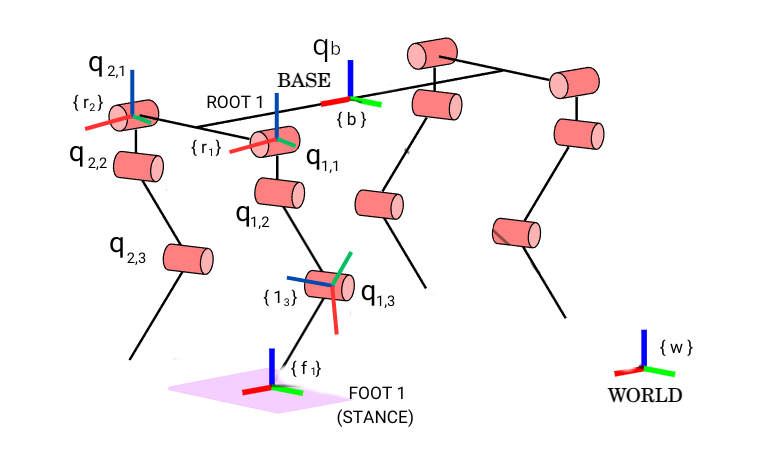
\includegraphics[width=0.9\textwidth]{Images/img_ch2/LeggedCoordinates.png}
    \caption{\cite{FloatingBase1} Quadruped kinematic model}
    \label{fig:LeggedCoordinates}
\end{figure}

As introduced in the previous section, in legged robots the base moves in the world frame. In legged locomotion \cite{QuadrupedLocomotion}, there are two main problems: 
\begin{enumerate}
    \setlength\itemsep{-0.7em} 
    \item Feet positioning to perform the gait
    \item Base positioning to maintain stability 
\end{enumerate}
These two problems introduce two different kinematic objectives, discussed briefly here.

\textbf{Problem 1: Feet positioning}

Estimation of the base pose in
the world is known as \textbf{localization} problem\cite{ProbabilisticRobotics}\cite{LeggedLocalization}(present in any mobile robot), which is outside of the scope of this research.
Furthermore, motion is achieved by a discrete placement of feet along the path. The problem of \textbf{path planning}\cite{LeggedPlanning1} requires the definition of each foot stance position. 
This concept is discussed in \ref{sec:leggedControl}, for now, it is important to anticipate that to achieve legged locomotion, foot position is usually computed in the base frame \textbf{b}. 

For those reasons, this forward kinematic problem consists of deriving the pose of each foot tip $\mathbf{f_j}$ in the base frame \textbf{b} ($\mathbf{T^b_{f_j}}$) (sometimes in the world \textbf{w} frame,$\mathbf{T^w_{f_j}}$).  
Knowing the pose of the base \textbf{b} in the world \textbf{w} ($\mathbf{T^w_b}$), and all joint variables $\mathbf{q_j}$ of each leg j.


Under this hypothesis, the \textbf{floating base} model \cite{FloatingBase2}\cite{LeggedThesis} is used. The base pose introduce 6 additional DOFs in 3D, $\mathbf{q_b} = \begin{bmatrix}
        x_b & y_b & z_b & \vartheta_b & \varphi_b & \psi_b
    \end{bmatrix}^T $ 
included in the system DOFs $\mathbf{q_{tot}} = \begin{bmatrix}
        \mathbf{q} & \mathbf{q_b}
    \end{bmatrix}^T \in \mathbb{R}^{n+6}$.
$\mathbf{q_b}$ affect the system state but there isn't any dedicated actuator, so they are considered as unactuated virtual DOFs (see Fig.\ref{fig:FloatingBase}).  

\begin{figure}[H]
    \centering
    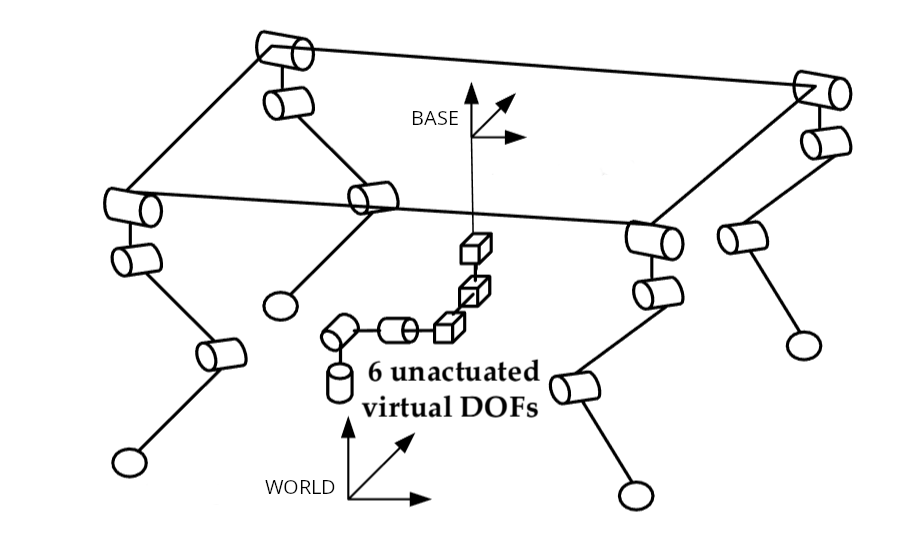
\includegraphics[width=0.6\textwidth]{Images/img_ch2/FloatingBase_2.png}
    \caption{Floating base model}
    \label{fig:FloatingBase}
\end{figure}

Refering to Fig.\ref{fig:FramesLegged}, to derive $\mathbf{T^b_{f_j}}$ an equation similar to \ref{eq:FKTITAN4} is used: 
\begin{equation}
\label{eq:FKLEG}
    \mathbf{T^b_{f_j}(q_j)} = \mathbf{T^b_r} \cdot \mathbf{T^r_{j_0}}\cdot \mathbf{T^{j_0}_{j_1}(q_{j,1})}  \dots \cdot \mathbf{T^{j_{i-1}}_{j_i}(q_{j,i})} \dots \cdot \mathbf{T^{j_{{n_j}-1}}_{j_{n_j}}(q_{j,{n_j}})}\cdot \mathbf{T^{j_{n_j}}_{f_j}}
    , \forall j=1,...,N
\end{equation}

If instead the foot position in the world frame is needed, the floating base DOFs are used
\begin{equation}
\label{eq:FKLEG}
    \mathbf{T^w_{f_j}(q_j, q_b)} = \mathbf{T^w_b(q_b)} \cdot \mathbf{T^b_{f_j}(q_j)}
    , \forall j=1,...,N
\end{equation}

\begin{figure}[H]
    \centering
    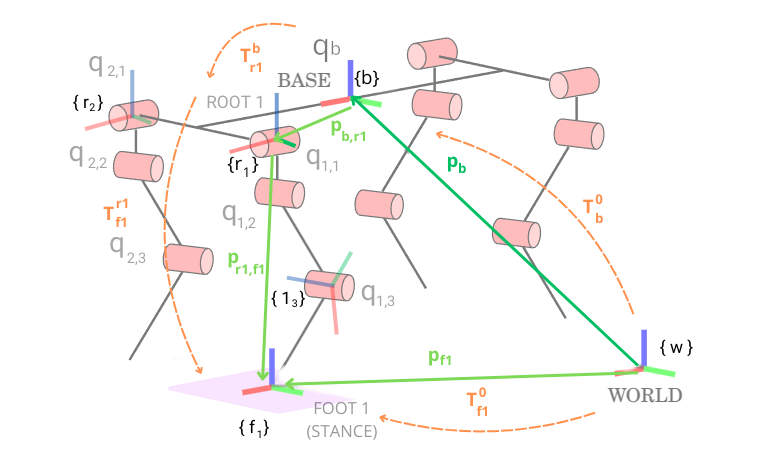
\includegraphics[width=1.0\textwidth]{Images/img_ch2/FramesLegged.png}
    \caption{Floating base kinematic position vectors}
    \label{fig:FramesLegged}
\end{figure}


\textbf{Problem 2: Base positioning}

In a legged machine, stability is a crucial aspect, explored in detail in \ref{ch:chapter_three}. For now, take for granted that to maintain the base stable, the base CoM is positioned in a specific region from the stance feet contact points. For this reason, it is important to describe the pose of the base from each foot contact point frame $\mathbf{T^{f_j}_b}$.

This forward kinematic problem consists of the derivation of the base pose \textbf{b} respect each contact leg foot $\mathbf{f_j}$ ($\mathbf{T^{f_j}_b}, \forall j \in J_c$), given the vector of leg $j$ DOFs $\mathbf{q_j}$.
Where $J_c$ defines the set of indices of legs in contact with the ground.

The kinematic model of each contact leg $j \in J_c$ is redefined for this purpose from the foot tip to the leg root as in Fig.\ref{fig:LegReversedKinModel}. 
Contact with the ground is assumed to take place such that the ground can exert only a “pushing” force on each leg but no moment. Thus, while we can model the contact between leg and ground as a spherical joint, care must be
taken so that no pulls of the ground on the leg are required for a given gait\cite{RoboticMechanics}
(The above assumption excludes climbing and complex multi-limb robot structures).

In this model, each contact foot frame $\mathbf{f_j}$ is attached to the foot tip and considered aligned with the ground in the xy plane. The spherical joint models the ground interaction and is represented by 3 rotational DOFs ($q_{j,1}, q_{j,2}, q_{j,3}$) of virtual unactuated joint variables (as for the floating base). 
The derivation of $\mathbf{T^{f_j}_b}$ is just a matter of homogeneous transformation composition as already described in depth:
\begin{equation}
\label{eq:FKLEG2}
    \mathbf{T^{f_j}_b(q_j)} = \mathbf{T^{f_j}_{j_1}(q_{j,1})} \cdot \mathbf{T^{j_1}_{j_2}(q_{j,2})} \cdot \cdot \mathbf{T^{j_{i-1}}_{j_i}(q_{j,i})} \dots \cdot \mathbf{T^{j_{n_{j}-1}}_{j_{n_{j}}}(q_{j,n})}\cdot \mathbf{T^{j_{n_{j}}}_{r_j}}\cdot \mathbf{T^{r_j}_b}
    , \forall j \in J_c
\end{equation}

\begin{figure}[H]
    \centering
    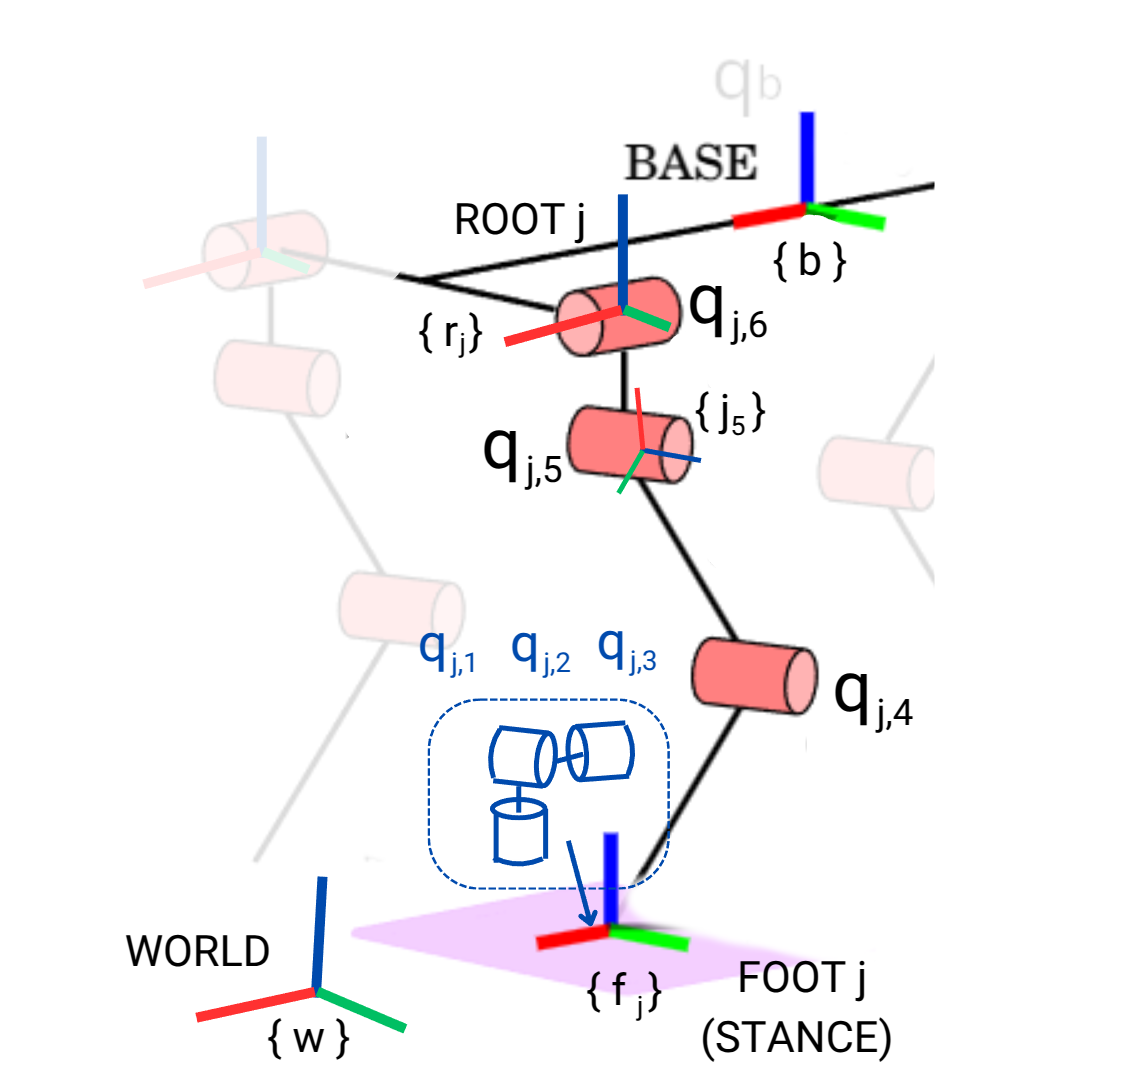
\includegraphics[width=0.6\textwidth]{Images/img_ch2/LegModeltiproot.png}
    \caption{Kinematic model of stance leg from foot tip to leg root}
    \label{fig:LegReversedKinModel}
\end{figure}

\subsubsection{Limbed Robots, Multipurpose Machines}
\label{sec:limbedFK}
From some limbed robots described in chapter \ref{ch:chapter_one}, the multifunctional aspect is clear.  
Those robots can move with walking locomotion, but also climbing, hybrid legged-wheeled driving, and even manipulate objects in the meantime\cite{SCAR-E}\cite{Koyachi}\cite{WheelLeggedStabilityOPT}. 
As for the kinematic modeling of walking machines defined in the previous section, different problems have to be solved. In general, we are interested in: 
\begin{itemize}
    \setlength\itemsep{-0.7em} 
    \item All limbs-end position respect base (or world) 
    \item Base pose respect limb-end 
\end{itemize}

The kinematic model for a generic multi-limb robot is as the one in Fig.\ref{fig:MultiLimbKin}.
The frames have the same meaning as for walking robots, except for the last frame referred to as $\mathbf{e_j}$. As for manipulators, any manipulation or locomotion "tool" can be attached to each limb's end frame (spine gripper, magnetic gripper, manufacturing tool, wheel, and so on...). 

\begin{figure}[H]
    \centering
    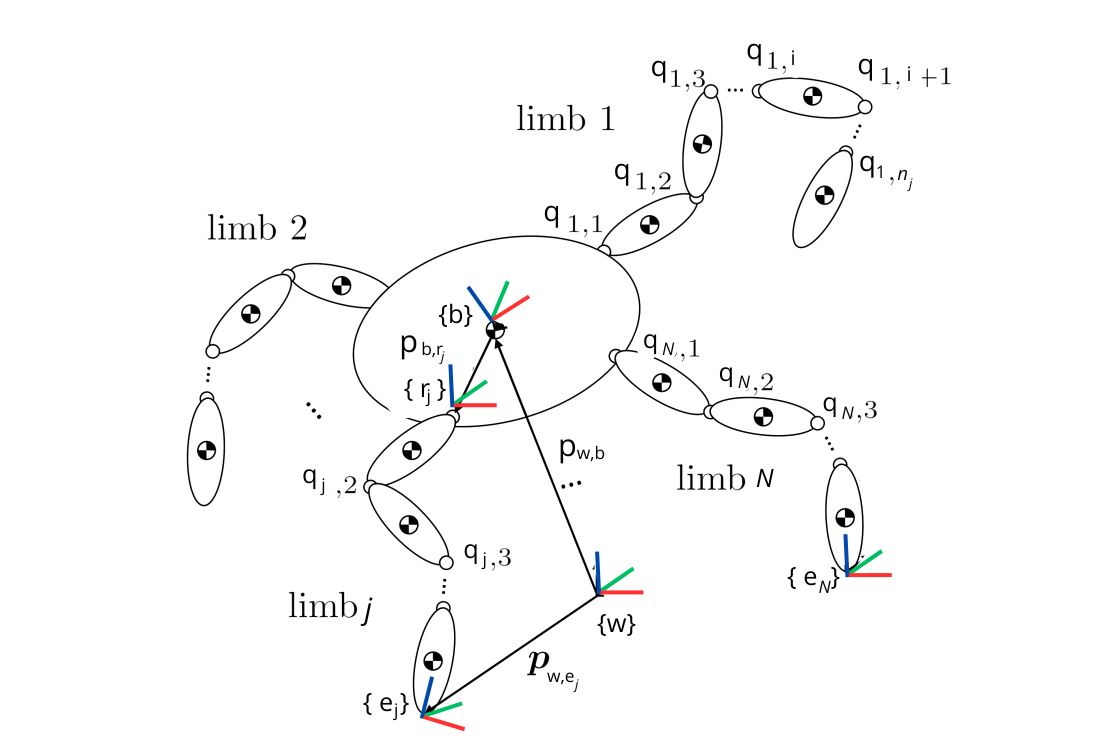
\includegraphics[width=0.85\textwidth]{Images/img_ch2/MultiLimbKin.png}
    \caption{\cite{Ribeiro2023reaction} model of multi-limb robot}
    \label{fig:MultiLimbKin}
\end{figure}

To solve the two main forward kinematic problems listed above, the same resolution as in equation \ref{eq:FKLEG2} (limb-end to base)and \ref{eq:FKLEG} (base to limb-end) can be applied. 


\newpage
Figure \ref{fig:FkAll} below summarizes the different robots' FK problems described here.
\begin{figure}[H]
    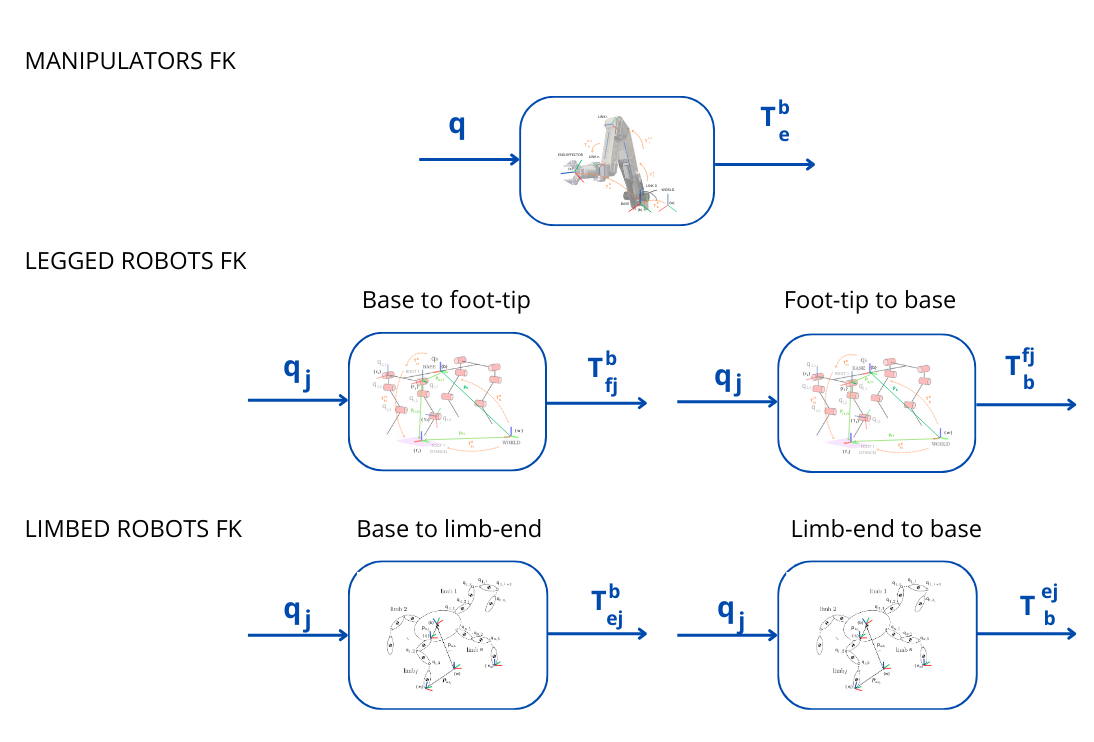
\includegraphics[width=1.1\textwidth, inner]
    {Images/img_ch2/FK_ALL.png}
    \caption{Scheme of FK problem for different robots}
    \label{fig:FkAll}
\end{figure}

With a standard procedure, the homogeneous transformation matrix is a way to represent the "final" frame pose. From that matrix, it is possible to extract the explicit FK equation $k(\cdot)$ in the task space. Alternatively, geometric analysis is always possible, but there isn't a standard formulation procedure.   

\subsection{Inverse Kinematic}
\label{sec:inverse}
As the name suggests, IK solves the Inverse problem of FK, going from the final frame pose (or task space) to the joint space \cite{Siciliano}\cite{RoboticMechanics}(as represented in Fig.\ref{fig:IKScheme}). 
From \cite{Siciliano}, in the context of \textbf{Manipulators}:
\textit{"The inverse kinematics problem consists of
the determination of the joint variables corresponding to a given end-effector position and orientation. The solution to this problem is of fundamental importance to transform the motion specifications, assigned to the end-effector in the operational space, into the corresponding joint space motions that allow execution of the desired motion"}.
So, in this formulation for different robotic structures, the "end-effector" could be the mobile base of the legged/limbed robot or the limb/leg end, depending on the task to execute.
\begin{figure}[H]
    \centering
    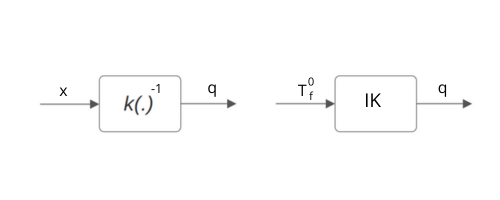
\includegraphics[width=0.7\textwidth]
    {Images/img_ch2/IKScheme.png}
    \caption{Scheme of general IK problems}
    \label{fig:IKScheme}
\end{figure}

Figure \ref{fig:IkAll} tries to summarize the IK problem for different robots with a simple scheme.
\begin{figure}[H]
%\hspace{-2cm} 
    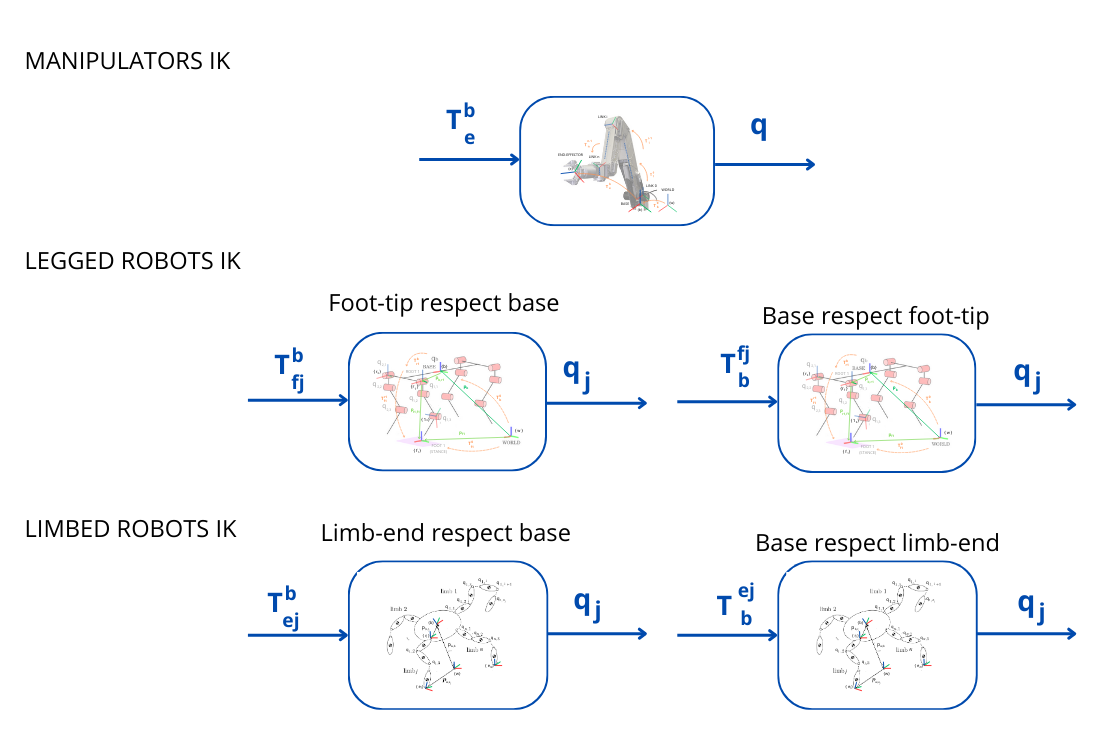
\includegraphics[width=1.1\textwidth, inner]
    {Images/img_ch2/IK_ALL.png}
    \caption{Scheme of FK problem for different robots}
    \label{fig:IkAll}
\end{figure}

\newpage
While FK has always one (and only one) solution, IK can have one, multiple (even infinite), or no solutions.

From the definition of workspace \ref{def:workspace}, it is clear that if a pose outside of it is chosen, IK cannot be solved. Due to mechanical constraints, link collisions, or design choice, the joint space $\mathbf{q} \in \mathbb{R}^n$ is an ideal space. The counter-image of the workspace is a subspace of the joint space, this can be defined as constrained joint space $\mathbf{\bar{q}} \subseteq \mathbf{q}$.
For example, for a single revolute joint mechanism, the joint space is $\mathbf{q} \in \mathbb{R}$, but if it can move only in between $-\pi$, $\pi$, then the constrained joint space is $\mathbf{\bar{q}} \in [-\pi, \pi]$.

There isn't a standard way to solve IK, some techniques are: 
\begin{itemize}
\item \textbf{FK algebraic inversion}:\newline
It consists of deriving the FK solution and inverting it.
But, whenever revolute joints are involved, it is clear that trigonometric functions of the joint variables appear in FK, not invertible in $\mathbf{\bar{q}}$.
Then, to invert it, assumptions on the constrained joint space domain are needed. Depending on the domain restriction, different solutions are found.
Even when a solution exists, finding a closed-form IK solution is hard and sometimes not possible. 
Having a closed-form solution makes computation faster and more reliable, expressed as: 
\begin{equation}
\label{eq:IK}
    \mathbf{q} = f_{IK}(\mathbf{x_f})
\end{equation}
Where $\mathbf{x_f}$ denotes the final frame task space vector.
When it is not possible, numerical methods are used.
\item \textbf{Numerical methods}:\newline
To solve non-linear equations, numerical methods such as Newton-Raphson\cite{ModernRobotics} are often used in robotics.
\item \textbf{Inverse differential kinematics}:\newline
This solution depends on the differential kinematic formulation, which will be discussed in section\ref{sec:differential}. For IK solution, once an explicit velocity relation is established between joint space and final frame velocity (goal of DK), it is inverted and integrated. 
\end{itemize}

Next, an overview of the IK problem for the robotics structure of interest is done. However, due to the absence of a standard method, the details of the resolution are not addressed here. 

\subsubsection{Manipulators and Single-Leg/Limb}
\label{sec:manipulatorIK}
The problem of IK for manipulators has already been introduced, formally: \\
\textit{Given a desired end-effector pose $\mathbf{T^0_e}$ ($\mathbf{T^w_e}$),or as $\mathbf{x}$, derive the joint configuration $\mathbf{q}$ to reach it.}



Again, as for FK, the same approaches can be used for single legs/limbs modeled from the base root attachment to the tip/end.
In that case, the problem is formulated as follows:\newline 
\textit{Given a desired limb $j$-end/leg $j$-tip  pose $\mathbf{T^b_{f_j/e_j}}$ ($\mathbf{T^w_{f_j/e_j}}$),or as $\mathbf{x_{f_j/e_j}}$, derive the joint configuration $\mathbf{q_j}$ to reach it.}

The IK problems described above are represented in Fig.\ref{fig:ArmLegIK}.
\begin{figure}[H]
    \centering
    \subfloat[\label{fig:ArmIK}]{
        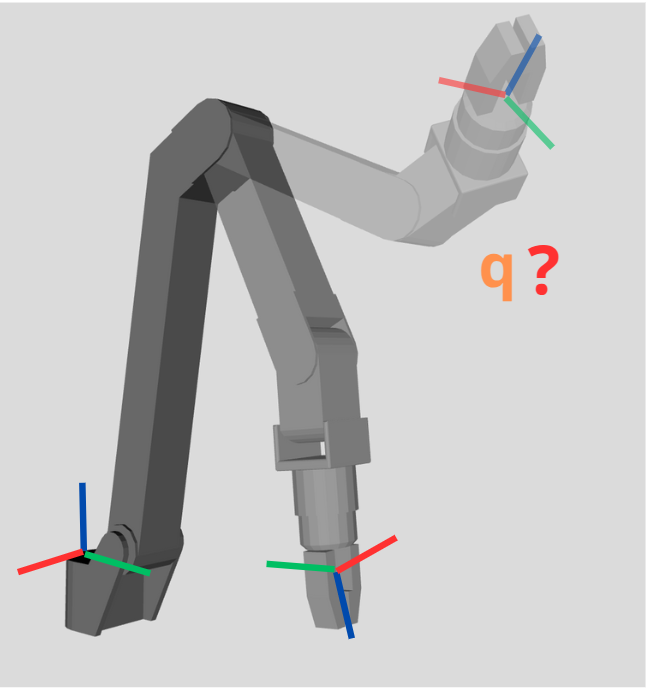
\includegraphics[scale=0.25]{Images/img_ch2/ArmIK.png}
    }
    \subfloat[\label{fig:LegIK}]{
        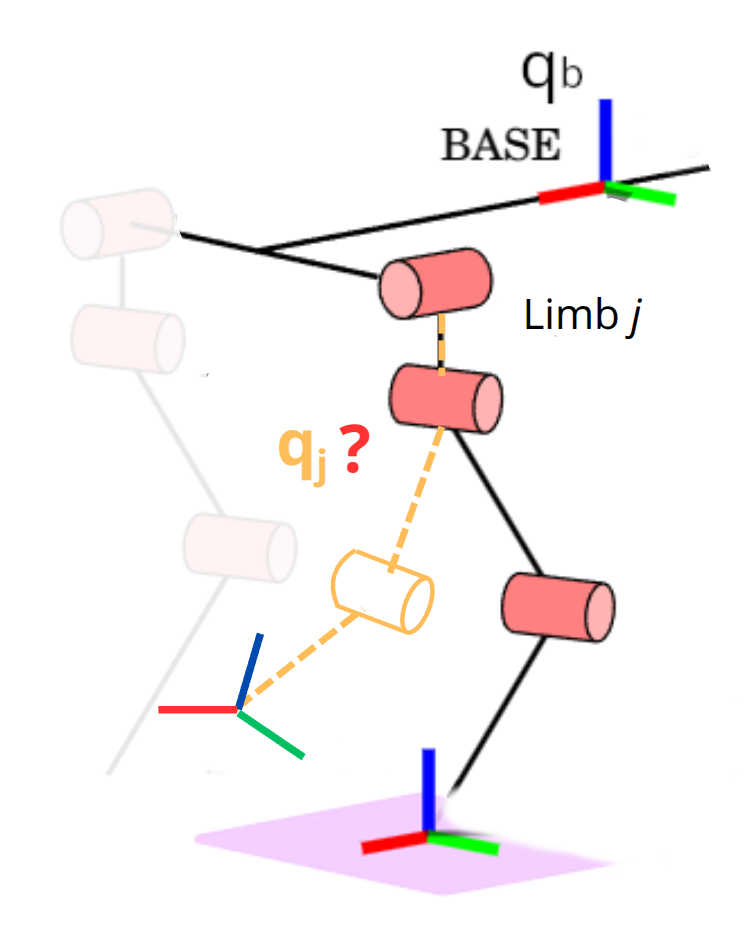
\includegraphics[scale=0.20]{Images/img_ch2/LegIK.png}
    }
    \caption[Leg/Limb and Arm IK]{IK problem for Manipulators (a) and single leg/limb (b)}
    \label{fig:ArmLegIK}
\end{figure}

The resolution of the IK described above is needed to plan any arm/limb manipulation or single leg/limb step. A different approach is used when positioning a legged/limb robot base. 
The definition of this IK problem is described in the next part. 

\subsubsection{Legged/Limbed Robots Base}
\label{sec:leggedLimbedIK}
The representation in Figure \ref{fig:IkAll} of IK for legged/limbed robots base is not complete. 
In fact, when dealing with base motion, we can reformulate the problem as: \newline
\textit{The inverse kinematics problem consists of
the determination of \textbf{all} legs/limbs joint variables corresponding to a given base position and orientation. The solution to this problem is of fundamental importance to transform the motion specifications, assigned to the base frame, into the corresponding joint space motions that allow execution of the desired motion.}

The relation to derive is not the single leg/limb mapping from
$\mathbf{T^{f_j/e_j}_w}$ to $\mathbf{q_j}$. To position the base, a \textbf{closed chain} structure (as in Fig.\ref{fig:closedkin}) is considered. Only legs/limbs in contact with the ground ($j \in J_c$) affect base positioning.

Formally: 
\textit{Given a desired base pose $\mathbf{T^{f_j/e_j}_b}$ (from one of the contact legs/limbs $j\in J_c$ frames), derive all contact legs/limbs joint configurations $\mathbf{q_c} \subseteq \mathbf{q}$ to reach it.}

Here, two approaches are described, in both cases, rigid contact with the ground is assumed for the kinematic modeling.
The first does not directly consider the closed chain, instead considers no penetration constraint of contact legs/limbs tip. 
The second instead relies on the parallelogram kinematic model to formalize and solve IK. 

\textbf{Contact Leg/limb Motion Propagation without Penetration}\newline 
When the contact between leg/limb-tip and ground is rigid, if a motion occurs during contact, ground penetration is not possible. This causes a motion propagation towards the root, rigidly attached to the base. CConsidering only translational motion of the limb/leg in contact $j \in J_c$, if motion along 3D vector $\mathbf{v_{e_j/f_j}} = \begin{bmatrix}
\mathbf{x_{e_j/f_j}} & \mathbf{y_{e_j/f_j}} & \mathbf{z_{e_j/f_j}}\end{bmatrix}^T $
this is mapped into a limb/leg root motion $\mathbf{v_{r_j}} = -\mathbf{v_{e_j/f_j}}$. 
According to rigid body theory \cite{RoboticMechanics}, the motion is translational when all points move along parallel directions, otherwise it is rotational.  
Therefore, when all contact legs/limbs roots translate along the same direction, that motion is propagated to the robot base. For a base rotation, different root translations are combined.

In simple terms, positioning the base becomes a problem of contact legs/limbs position, using the same single root-to-tip model described before. 

This approach is formulated in terms of "motion" and "changes in position", which is a topic of differential kinematics (treated in the next section). But it remains an IK problem if interpreted with the following steps:
\begin{enumerate}
    \setlength\itemsep{-0.7em} 
    \item Select a desired base pose $\mathbf{T^{f_j/e_j}_b}$ to $\mathbf{q_j}$.
    \item Convert that pose as the configuration of contact legs $\mathbf{T^b_{f_j/e_j}}, \forall j \in J_c$. 
    \item Solve leg/limb IK $\forall j \in J_c$.
\end{enumerate}


Figure \ref{fig:BaseMotionIK} represents some examples of legs/limbs to base motion conversion. 

\begin{figure}[H]
    \subfloat[Z translation.\label{fig:MoveBaseUP}]{
        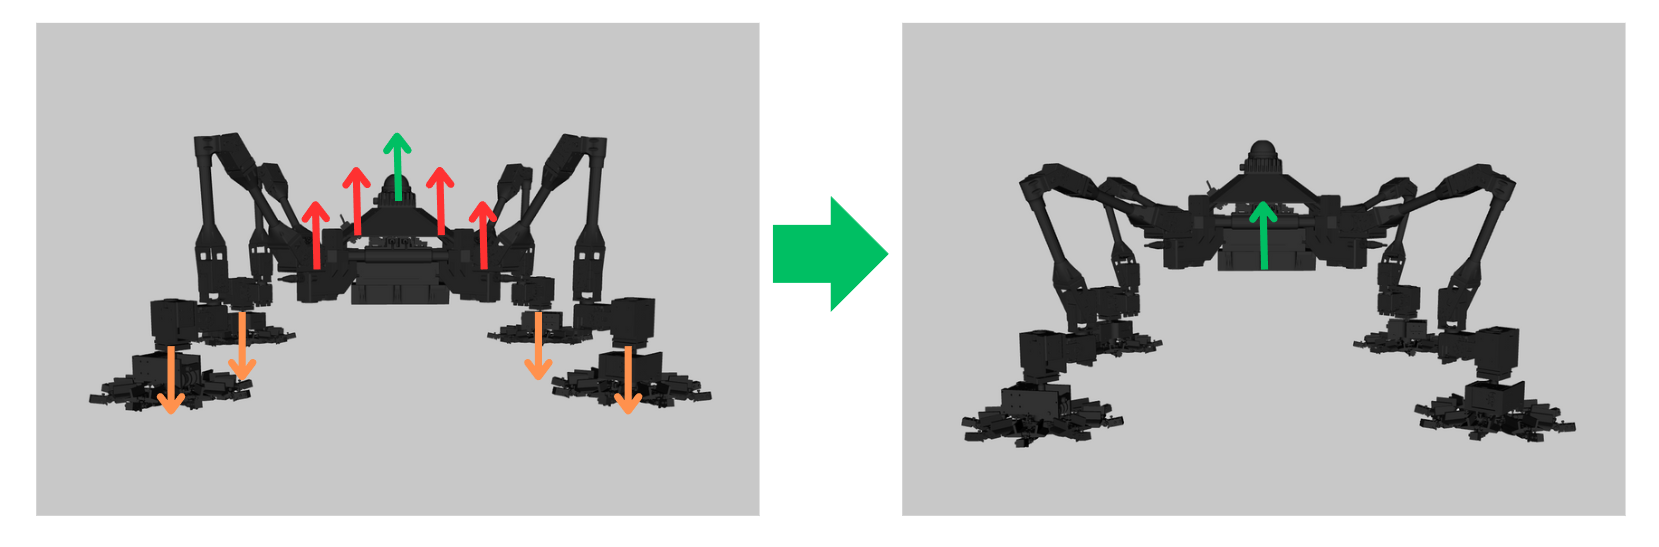
\includegraphics[scale=0.25]{Images/img_ch2/MoveBaseUP.png}
    }
    \quad
    \subfloat[XY translation.\label{fig:MoveBaseBACK}]{
        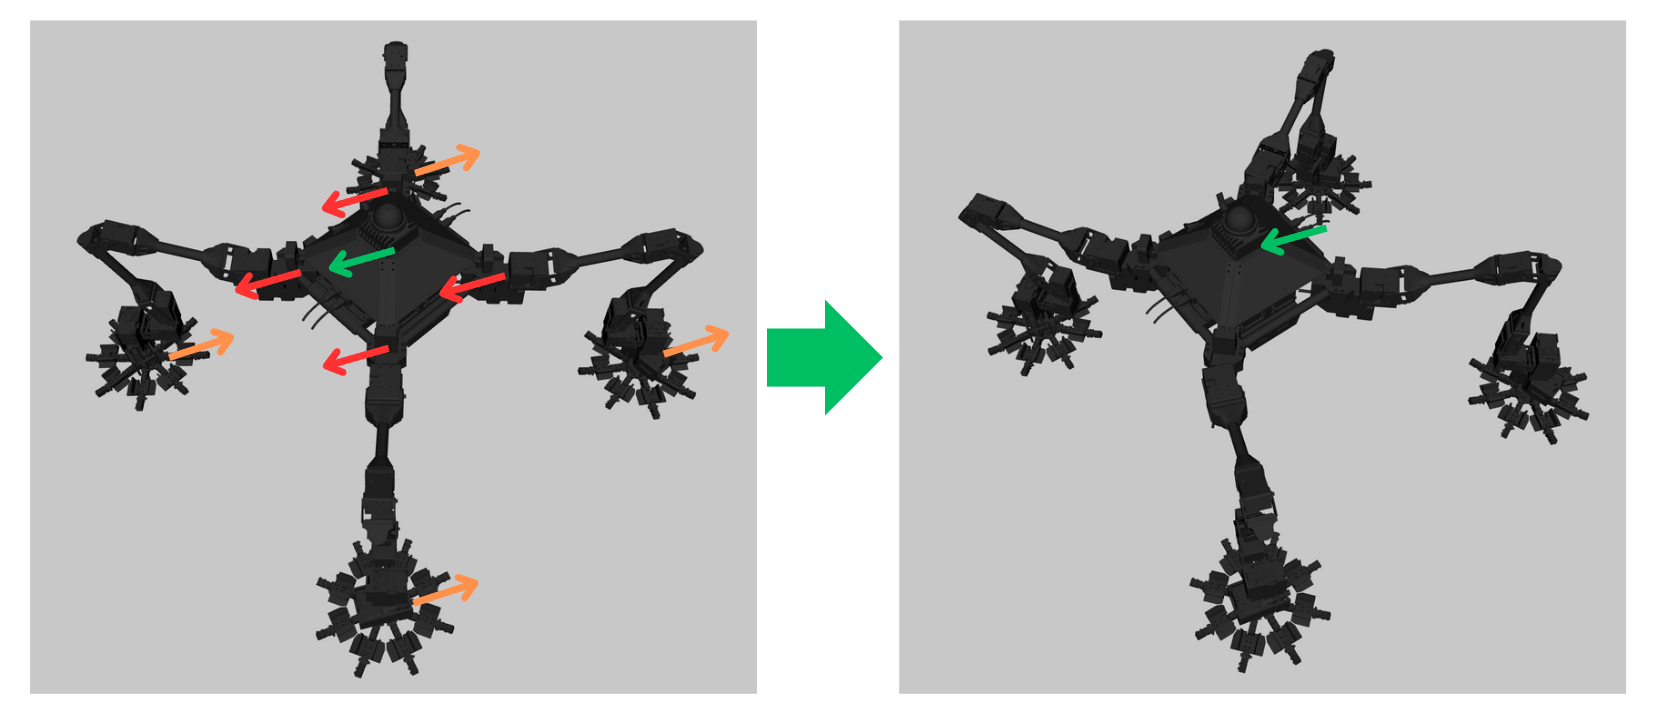
\includegraphics[scale=0.25]{Images/img_ch2/MoveBaseBACK.png}
    }
    \quad
    \subfloat[Yaw rotation.\label{fig:MoveBaseZRotate}]{
        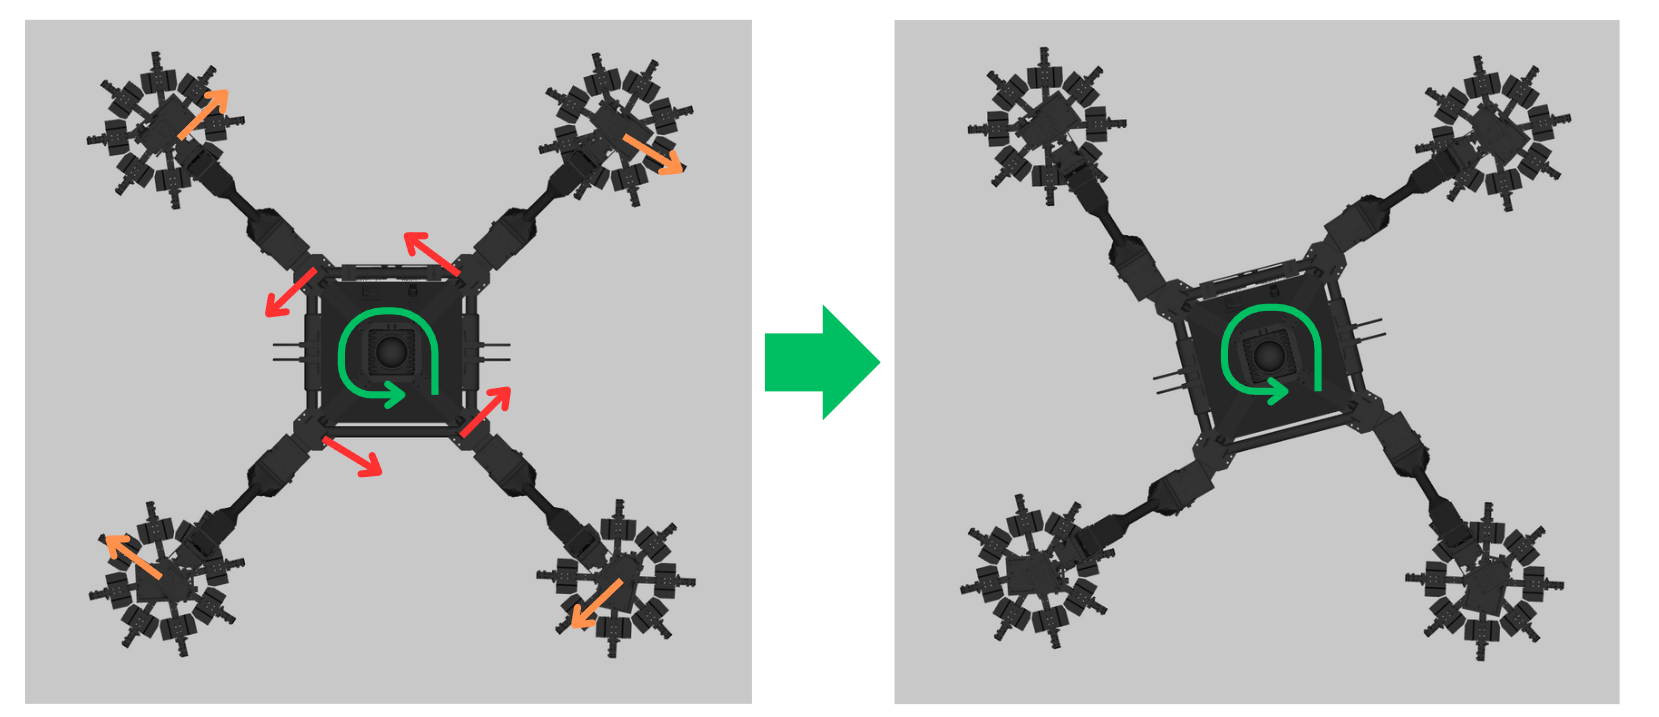
\includegraphics[scale=0.25]{Images/img_ch2/MoveBaseZRotate.png}
    }
    \caption[Limbed Robot IK Motion]{Different base motion as limb motion task. Orange arrows are objective limb position, reds are the new corresponding root pose, and green is the change on the base pose}
    \label{fig:BaseMotionIK}
\end{figure}


\textbf{Parallel Manipulator Model}\newline
Unlike serial manipulators (open chain structures as Fig.\ref{fig:Manipulator}), their parallel counterparts are composed of kinematic
chains with closed subchains (as in Fig.\ref{fig:ParallelManipulator} below).
Two frames can be distinguished, one fixed to the ground,\textit{B}, and one capable of moving arbitrarily within its workspace, \textit{M}.

\begin{figure}[H]
    \centering
    \subfloat[\cite{RoboticMechanics}Parallel manipulator scheme.\label{fig:Parallel}]{
        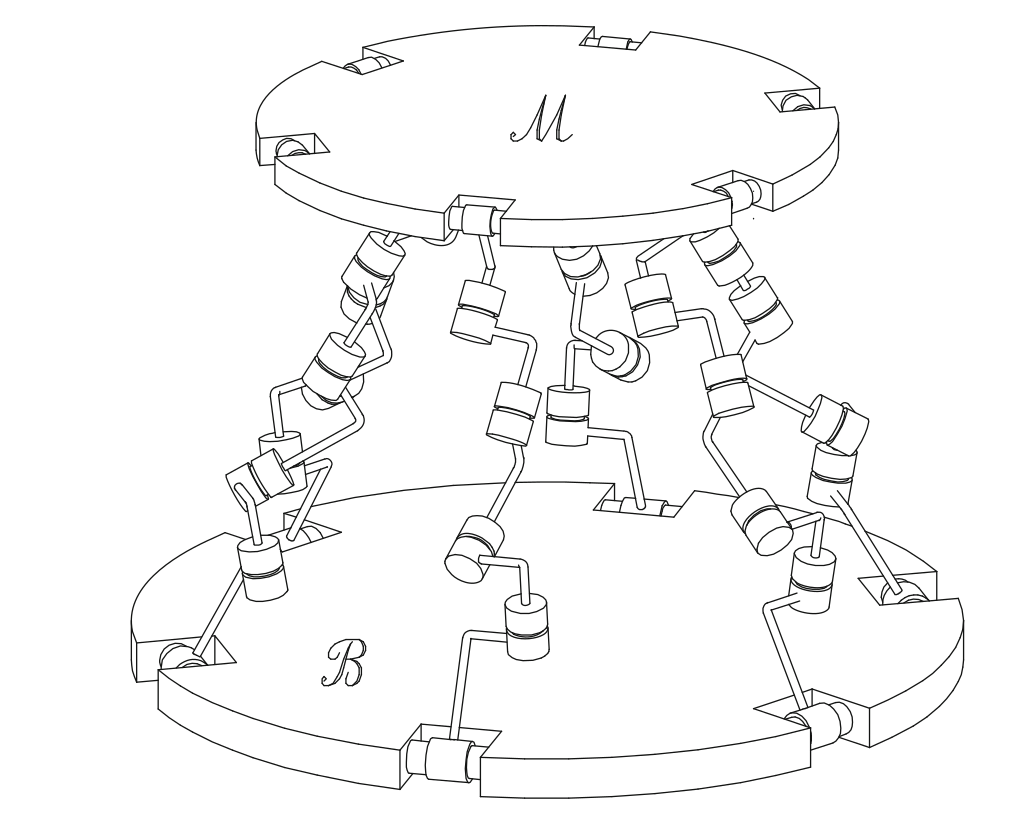
\includegraphics[scale=0.20]{Images/img_ch2/ParallelManipulator.png}
    }
    \subfloat[\cite{ABBParallel}ABB IRB.\label{fig:ABBParallel}]{
        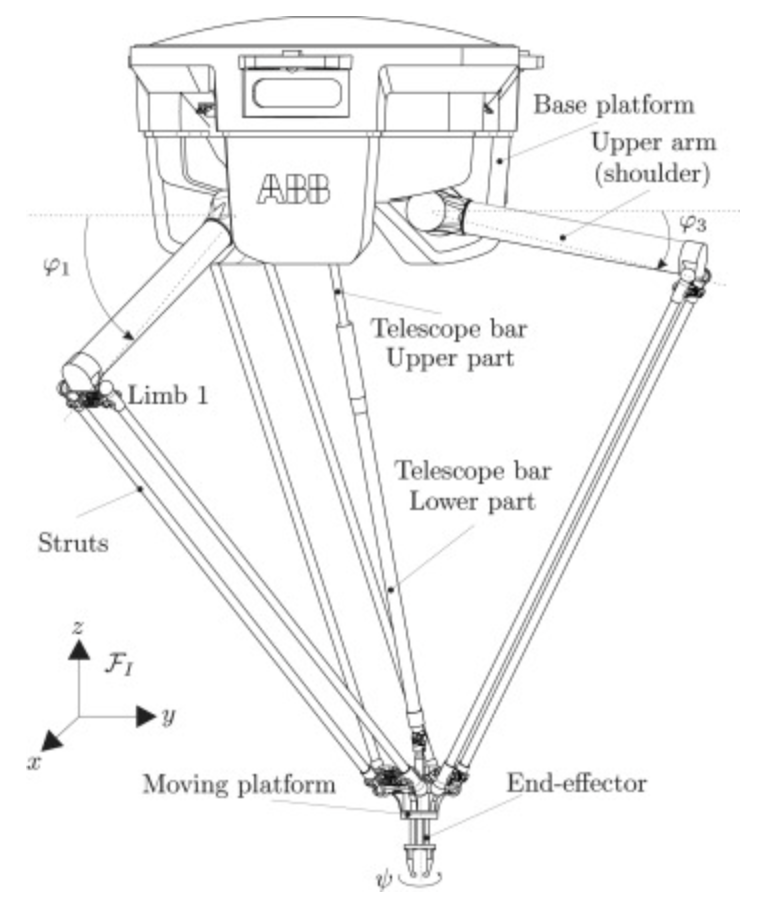
\includegraphics[scale=0.20]{Images/img_ch2/ABB_parallel.png}
    }
    \caption[Parallel Manipulator]{Parallel manipulator general scheme and example}
    \label{fig:ParallelManipulator}
\end{figure}

We can extend the parallel manipulator model\cite{RoboticMechanics} and consider the ground frame \textit{G} as fixed base (previously defined as \textit{B}), and the robot moving base \textit{B} as a moving frame (previously defined as \textit{M}) as in Fig.\ref{fig:KinematicWalkingParallel}.
Each leg is modeled from the contact point to the base root with the classical manipulator model described before. 
 

\begin{figure}[H]
    \centering
    \subfloat[Robot model as parallel manipulator.\label{fig:exapodparallel}]{
        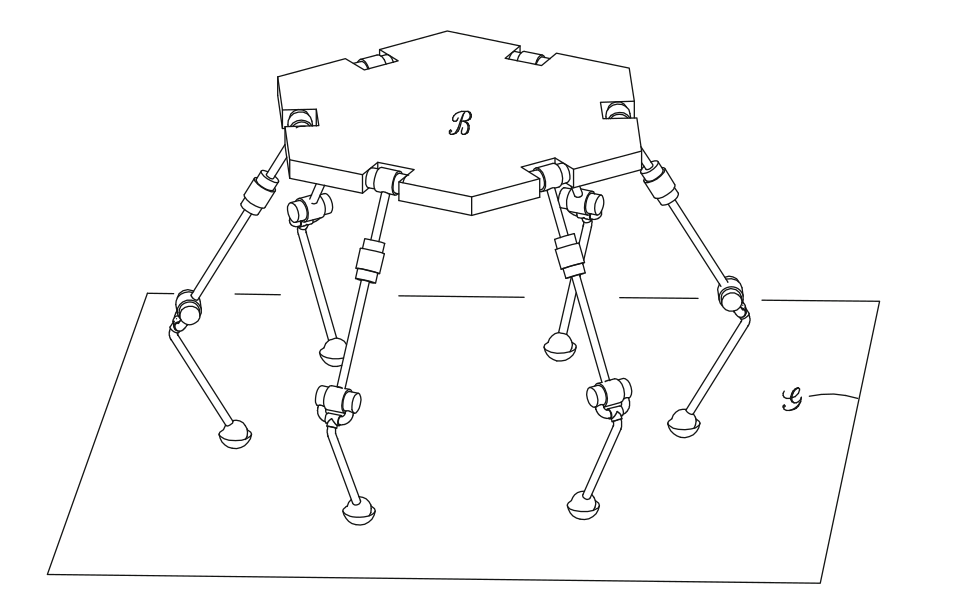
\includegraphics[scale=0.20]{Images/img_ch2/exapod_model.png}
    }
    \subfloat[Limb kinematic model.\label{fig:exapodleg}]{
        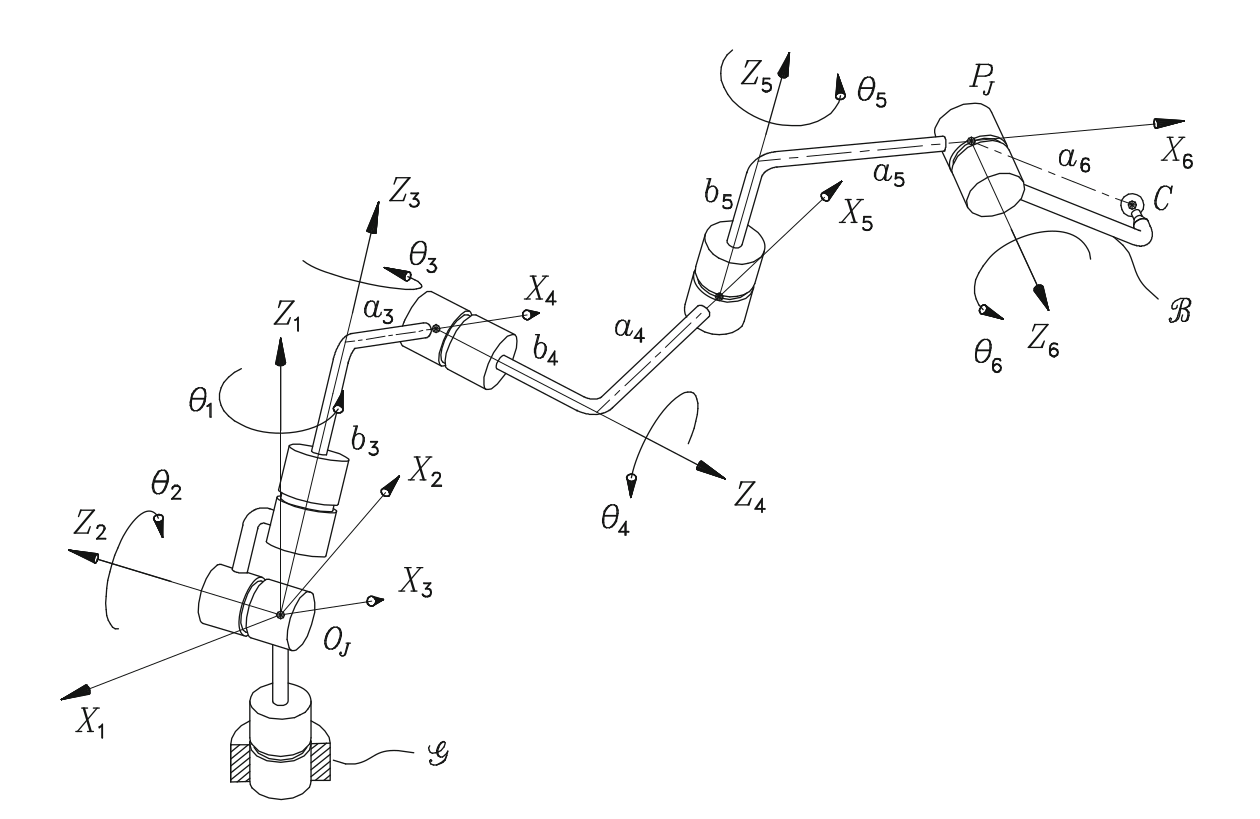
\includegraphics[scale=0.20]{Images/img_ch2/exapod_DH_leg.png}
    }
    \caption[Closed Kinematic chain Leg DH]{\cite{RoboticMechanics} Closed Kinematic chain base motion}
    \label{fig:KinematicWalkingParallel}
\end{figure}


When modeling legged robot base kinematics with the parallelogram structure, legs in contact with the ground are considered. 
Using the same leg kinematic model as in section \ref{sec:leggedFK}, The spherical joint of each leg j $q_{j,1}, q_{j,2},q_{j,3}$ accounts for the coupling of the leg with the ground. This is just for modeling purposes, there is no real actuation on those joints. So, we can reduce the space of actuated joint variables to  $\mathbf
{q_a} \in \mathbb{R}^{n-3N}$, removing all spherical coordinates.
A maneuver of \textit{B}, given by a prescribed pose, can be achieved by
suitable values of the contact limbs actuated-joints $\mathbf
{q_a}$ variables, which thus leads to a problem of parallel-manipulator inverse kinematics\cite{RoboticMechanics}.


\subsection{Differential Kinematic}
\label{sec:differential}
FK and IK have been defined as the direct and inverse mapping between joint space and task space. Such relations capture the robot configuration at a specific time instant. Differential kinematics (DK) instead derives the relationship between joint velocities and final frame linear $\mathbf{\dot{p}_f}$ and angular $\mathbf{\omega_f}$ velocity\cite{Siciliano}.
Denoting the joint space as $\mathbf{\dot{q}} \in \mathbb{R}^n$, and the final frame velocity vector
$\mathbf{v_f} =
\begin{bmatrix}
\mathbf{\dot{p}_f} & \mathbf{\omega_f}
\end{bmatrix}^T$, the mapping is described by: 
\begin{equation}
\label{eq:DK}
    \mathbf{v_f} = \mathbf{J(\mathbf{q})}\cdot\mathbf{\dot{q}} 
\end{equation}

$\mathbf{J(\mathbf{q})}$ is a $6\times n$ matrix, called \textbf{geometrical Jacobian}. This matrix relation can be decomposed into a linear and angular part: 
\begin{equation}
\label{eq:DK_decomposed}
    \mathbf{v_f} =
    \begin{bmatrix}
    \mathbf{\dot{p}_f}\\
    \mathbf{\omega_f}
    \end{bmatrix} = 
    \begin{bmatrix}
    \mathbf{J_P(\mathbf{q})}\\
    \mathbf{J_O(\mathbf{q})}    \end{bmatrix} \cdot \mathbf{\dot{q}} 
\end{equation}

As always, the reference frame is important.
If the notation is expanded, the jacobian matrix relating velocity of frame $\mathbf{f}$ in frame $\mathbf{0}$ can be denoted as $\mathbf{^0J_f}$.
The expression above represents the velocity of the final frame $\mathbf{v_f}$ in a chosen reference frame $\mathbf{0}$ . If velocity has to be represented in frame $\mathbf{k}$, it is easy to do under the hypothesis that $\mathbf{R^k_0}$ is constant \cite{Siciliano}\cite{CorkeMATLAB}. It holds: 

\begin{equation}
\label{eq:VelocityRelation}
    \mathbf{^k v_f} = \begin{bmatrix}
    \mathbf{^k\dot{p}_f}\\
    \mathbf{^k\omega_f}
    \end{bmatrix} =     \begin{bmatrix}
    \mathbf{R^k_0} & \mathbf{0_{3\times 3}}\\
    \mathbf{0_{3\times 3}} & \mathbf{R^k_0} 
    \end{bmatrix} \cdot    \begin{bmatrix}
    \mathbf{^0\dot{p}_f}\\
    \mathbf{^0\omega_f}
    \end{bmatrix} 
\end{equation}

Defining 
$\mathbf{J^k_0} = \begin{bmatrix}
    \mathbf{R^k_0} & \mathbf{0_{3\times 3}}\\
    \mathbf{0_{3\times 3}} & \mathbf{R^k_0} 
    \end{bmatrix}$
, representing a transformation of velocity frames from $\mathbf{0}$ to $\mathbf{k}$, from Eq.\ref{eq:DK}, it is possible to derive the expression of $\mathbf{^k v_f}$:
\begin{equation}
\label{eq:DKFrames}
    \mathbf{^k v_f} = \mathbf{J^k_0} \cdot \mathbf{J(q)} \cdot \mathbf{\dot{q}}
\end{equation}

From now on, the velocity reference frame is neglected, as it depends on the robotic structure under analysis. It will be made explicit only if necessary. 

When the final frame pose is represented in a minimal task space $\mathbf{x_f} \in \mathbb{R}^m$, it is possible to differentiate the forward kinematic relation, obtaining:
\begin{equation}
\label{eq:DK_analytical}
    \mathbf{\dot{x}_f} = \mathbf{J_a(\mathbf{q})}\cdot\mathbf{\dot{q}} 
\end{equation}

The \textbf{analytical Jacobian} $\mathbf{J_a(\mathbf{q})}$ is a $6\times m$ matrix, and in general it is different from the geometric one. 
The Jacobian, not only establishes velocity relation, but the inversion and integration of that relation give us an algorithm to solve IK. 
\begin{equation}
\label{eq:IKfromDK1}
    \mathbf{\dot{q}} = \mathbf{J^{-1}(\mathbf{q})}\cdot    \mathbf{v_f}  
\end{equation}
and then: 
\begin{equation}
\label{eq:IKfromDK2}
    \mathbf{q}(t) = \int_0^t{\mathbf{\dot{q}}(\varsigma)d\varsigma} + \mathbf{q}(0)  
\end{equation}
Obviously, techniques to avoid drifting errors of the integrator are implemented, but it is out of this scope. 

The importance of $ \mathbf{J(\mathbf{q})}$ to be invertible is clear from Eq.\ref{eq:IKfromDK1} . The values of $\mathbf{q}$ for which the Jacobian is not invertible ($det(\mathbf{J(\mathbf{q})}) = 0$, loss of rank) corresponds to a \textbf{singular configuration}. Singularities bring many problems, and so, the analysis of them is crucial for motion planning, and for system design.

The Jacobian matrix is also useful for understanding redundancy, an important concept in robotics, related to the relationship between joint space and task space\cite{Siciliano}\cite{RoboticMechanics}\cite{YoshikawaRedundancy}. A robot is redundant when the dimension of the task space $m$ is less than the joint space $n$, this brings additional freedom, but also complexity. 

Another tool derived from the Jacobian matrix is the \textbf{Manipuilability Ellipsoid} theory, widely expanded and used in this research. This is a geometric representation of the manipulability theory first introduced by T.Yoshikawa\cite{ManipulabilityYoshikawa}, where a hyper-spherical joint-space domain is mapped to a hyper-ellipsoidal task space, in the velocity or force: 
\begin{equation}
\label{eq:EllipsoidVel}
    \mathbf{\dot{q}}^T \mathbf{\dot{q}} = \mathbf{v_f}(\mathbf{J}\mathbf{J}^T)^{-1}\mathbf{v_f} = 1
\end{equation}
\begin{equation}
\label{eq:EllipsoidForce}
    \mathbf{\tau}^T \mathbf{\tau} = \mathbf{\gamma_e}^T(\mathbf{J}\mathbf{J}^T)\mathbf{\gamma_e} = 1
\end{equation}
This concept is expanded in Section \ref{sec:base_manipolability} for this research objective.

Finally, even if not related to kinematics, the Jacobian matrix provides a tool to solve the problem of \textbf{static}:
\textit{The goal of statics is to determine the relationship between the generalized
forces applied to the end-effector and the generalized forces applied to the joints (forces for prismatic joints, torques for revolute joints) with the
manipulator at an equilibrium configuration}\cite{Siciliano}.\\
The \textbf{kinetostatic duality} relationship can be proven with the principle of virtual work, deriving: 

\begin{equation}
\label{eq:Static}
\mathbf{\tau}  = \mathbf{J^T(\mathbf{q})}\cdot\mathbf{\gamma_{e}}
\end{equation}

where $\mathbf{\tau}\in \mathbb{R}^n$ is the vector of joint torques, and  $\mathbf{\gamma_{e}} \in \mathbb{R}^m$ is the vector of final frame generalized forces (force and moments) in task space. 

Again, there are some differences in the analysis of DK for manipulators and legged/limbed robots, which is explored in the next. 

\subsubsection{Manipulators and Single-Leg/Limb}
\label{sec:manipulatorDK}
For serial link structures like a manipulator or a single leg, DK relation is defined as in Eq.\ref{eq:DK}, with the same notation used for FK.
Fig.\ref{fig:ArmLegDK} represents an intuitive view of DK relation. 
If the frames are assigned using the DH convention, $\mathbf{J(\mathbf{q})}$ is derived column by column as: 
\begin{equation}
\label{eq:JacobianFormulaArm}
    \begin{bmatrix}
    \mathbf{j_{Pi}(\mathbf{q})}\\
    \mathbf{j_{Oi}(\mathbf{q})}    \end{bmatrix} = 
    \begin{cases}
    \begin{bmatrix}
    \mathbf{z_{i-1}}\\
    \mathbf{0}  \end{bmatrix}  \text{ if $i$ is prismatic}\\ \\ 
    \begin{bmatrix}
    \mathbf{z_{i-1}} (\mathbf{p_{e}} -  (\mathbf{p_{i-1}})\\
    \mathbf{z_{i-1}}\end{bmatrix} \text{ if $i$ is revolute}
    \end{cases}
\end{equation}

If the frames are not assigned with the DH convention, it is still possible to derive $\mathbf{J(\mathbf{q})}$ without this standard formulation.  
Furthermore, in terms of reference frame, Eq.\ref{eq:JacobianFormulaArm} provide the expression of $\mathbf{^b J_e(q)}$ (velocity of end-effector in base frame) or $\mathbf{^r J_f(q)}$ (velocity of foot/leg-tip in root frame), Eq.\ref{eq:DKFrames} is used for a change of reference frame (for example, to move to world \textbf{w} frame or legged/limbed body frame \textbf{b}).

The vectors in the statics equation \ref{eq:Static} in this case are: all the arm or leg/limb joint torques $\mathbf{\tau} \in \mathbb{R}^n$ and the generalized force applied at the end-effector or leg/limb-tip $\mathbf{\gamma_{e/f}} \in \mathbb{R}^m$.
For example, in 3D space it can be $m= 6$ and  $\mathbf{\gamma_{e/f}} = \begin{bmatrix}
    f_x & f_y & f_z & \mu_x & \mu_y & \mu_z
\end{bmatrix}^T$

\begin{figure}[H]
    \subfloat[DK of robotic arm.\label{fig:ArmDK}]{
    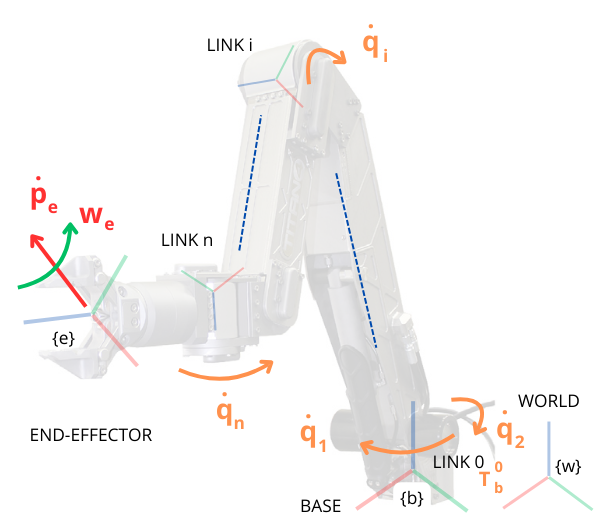
\includegraphics[scale=0.45]{Images/img_ch2/ArmDK.png}
    }
    \subfloat[DK of root-foot robotic leg/limb.\label{fig:LegDK}]{
        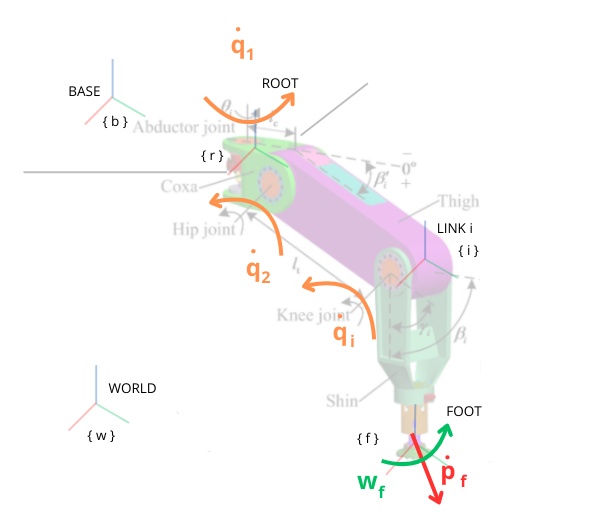
\includegraphics[scale=0.50]{Images/img_ch2/LegDK.png}
    }
    \caption[Arm and Leg/Limb DK]{Arm and Leg/Limb DK}
    \label{fig:ArmLegDK}
\end{figure}

\subsubsection{Legged/Limbed Robots Base}
\label{sec:leggedLimbedDK}
As discussed in the previous sections about FK and IK, the kinematics of N-legged/limbed robots involves the analysis of the base motion.
With reference to Fig.\ref{fig:LeggedDK},
the final goal is to derive a $6 \times n, (n=\sum_{j=1}^Nn_j)$ Jacobian matrix $\mathbf{J(q)}$ representing the relationship between
all legs/limbs joints velocity $\mathbf{\dot{q}} \in \mathbb{R}^n$ and the base velocity $\mathbf{v_b} = \begin{bmatrix}
\mathbf{\dot{p}_b} & \mathbf{\omega_{b}}\end{bmatrix}^T $ .

\begin{figure}[H]
    \centering
    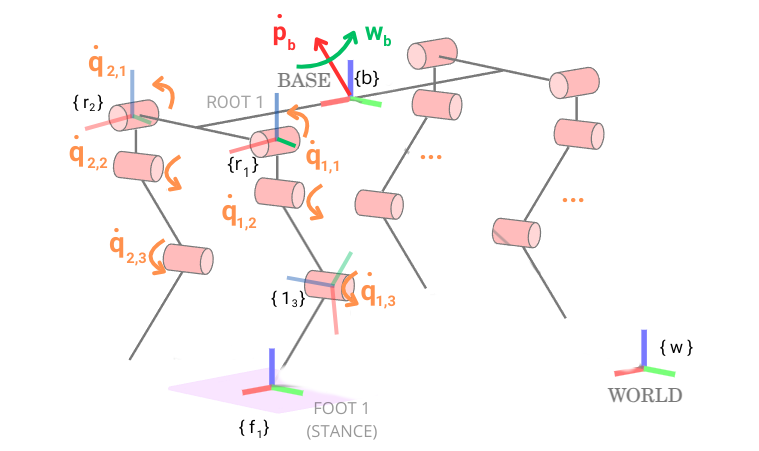
\includegraphics[width=0.9\textwidth]{Images/img_ch2/LeggedDK.png}
    \caption{Legged robot DK relation}
    \label{fig:LeggedDK}
\end{figure}

An alternative way to define the base velocity is $\mathbf{\dot{q}_b}$ through the \textbf{floating base model}, described previously. 

Different methods exist to derive this relationship, according to the kinematic model used. 
If the \textbf{parallel manipulator model} is used to describe the robot, theory on differential kinematics for closed chain structures exists \cite{Siciliano}\cite{RoboticMechanics}.
To define the contact point-to-root kinematic model, one of the two approaches expressed previously is possible: 
\begin{enumerate}
    \item Extend the leg/limb model with a spherical joint and model the system inverting joint order (used for the parallel manipulator model).
    \item use the contact leg/limb motion propagation without penetration approach, as defined in section\ref{sec:leggedLimbedIK}. 
\end{enumerate}

method (2) is employed in this thesis.
From now on, the Jacobian matrix and velocity vectors' reference frame is important, so it is explicit.
From the relation $\mathbf{^{e_j}v_{r_j}} = -\mathbf{^{r_j}v_{e_j/f_j}}$, it is just a matter of solving DK for the open chain root-to-tip leg/limb model (as in Eq.\ref{eq:DK}): 
\begin{equation*}
\label{eq:LegDKInversed1}
 \mathbf{^{r_j}v_{{e_j}/{f_j}}} = \mathbf{{^{r_j}J_j}(q_j)}\cdot\mathbf{\dot{q}_j}
\end{equation*}
so, with the velocity relation assumed before:
\begin{equation}
\label{eq:LegDKInversed2}
 \mathbf{^{e_j/f_j}v_{r_j}} = -\mathbf{{^{r_j}J_j}(q_j)}\cdot\mathbf{\dot{q}_j}
\end{equation}

The velocity vector $\mathbf{^{e_j/f_j}v_{r_j}}$ is equivalent to the velocity of one of the cooperative manipulators' end-effector (corresponding to the limb root), measured in its base frame (the contact foot/limb-tip). This parallelism is represented in Fig.\ref{fig:MultiArmLimbed}  

If we want to compute velocity of the limb root $\mathbf{^b v_{r_j}}$, measured on the base frame: 
\begin{equation}
\label{eq:rootDK_baseframe}
 \mathbf{^b v_{r_j}} = -\mathbf{J^b_{r_j}}\mathbf{{^{r_j}J_j}(q_j)}\cdot\mathbf{\dot{q}_j} = \mathbf{^b J_j(q_j)}\cdot\mathbf{\dot{q}_j}
\end{equation}

The ideas of \textbf{cooperative manipulators}\cite{CooperativeManipulators}\cite{DualArmManipulability}\cite{MultiArmManipulability} give a different point of view. Each leg/limb in contact with the ground $j \in J_c$ can be modeled from the contact point to the root as a separate "manipulator", cooperating to move the base frame. This is a novel approach for legged/limbed robots, introduced in this research, the details on this theory are addressed in in section \ref{sec:base_manipolability} of the next chapter.


\begin{figure}[H]
    \centering
    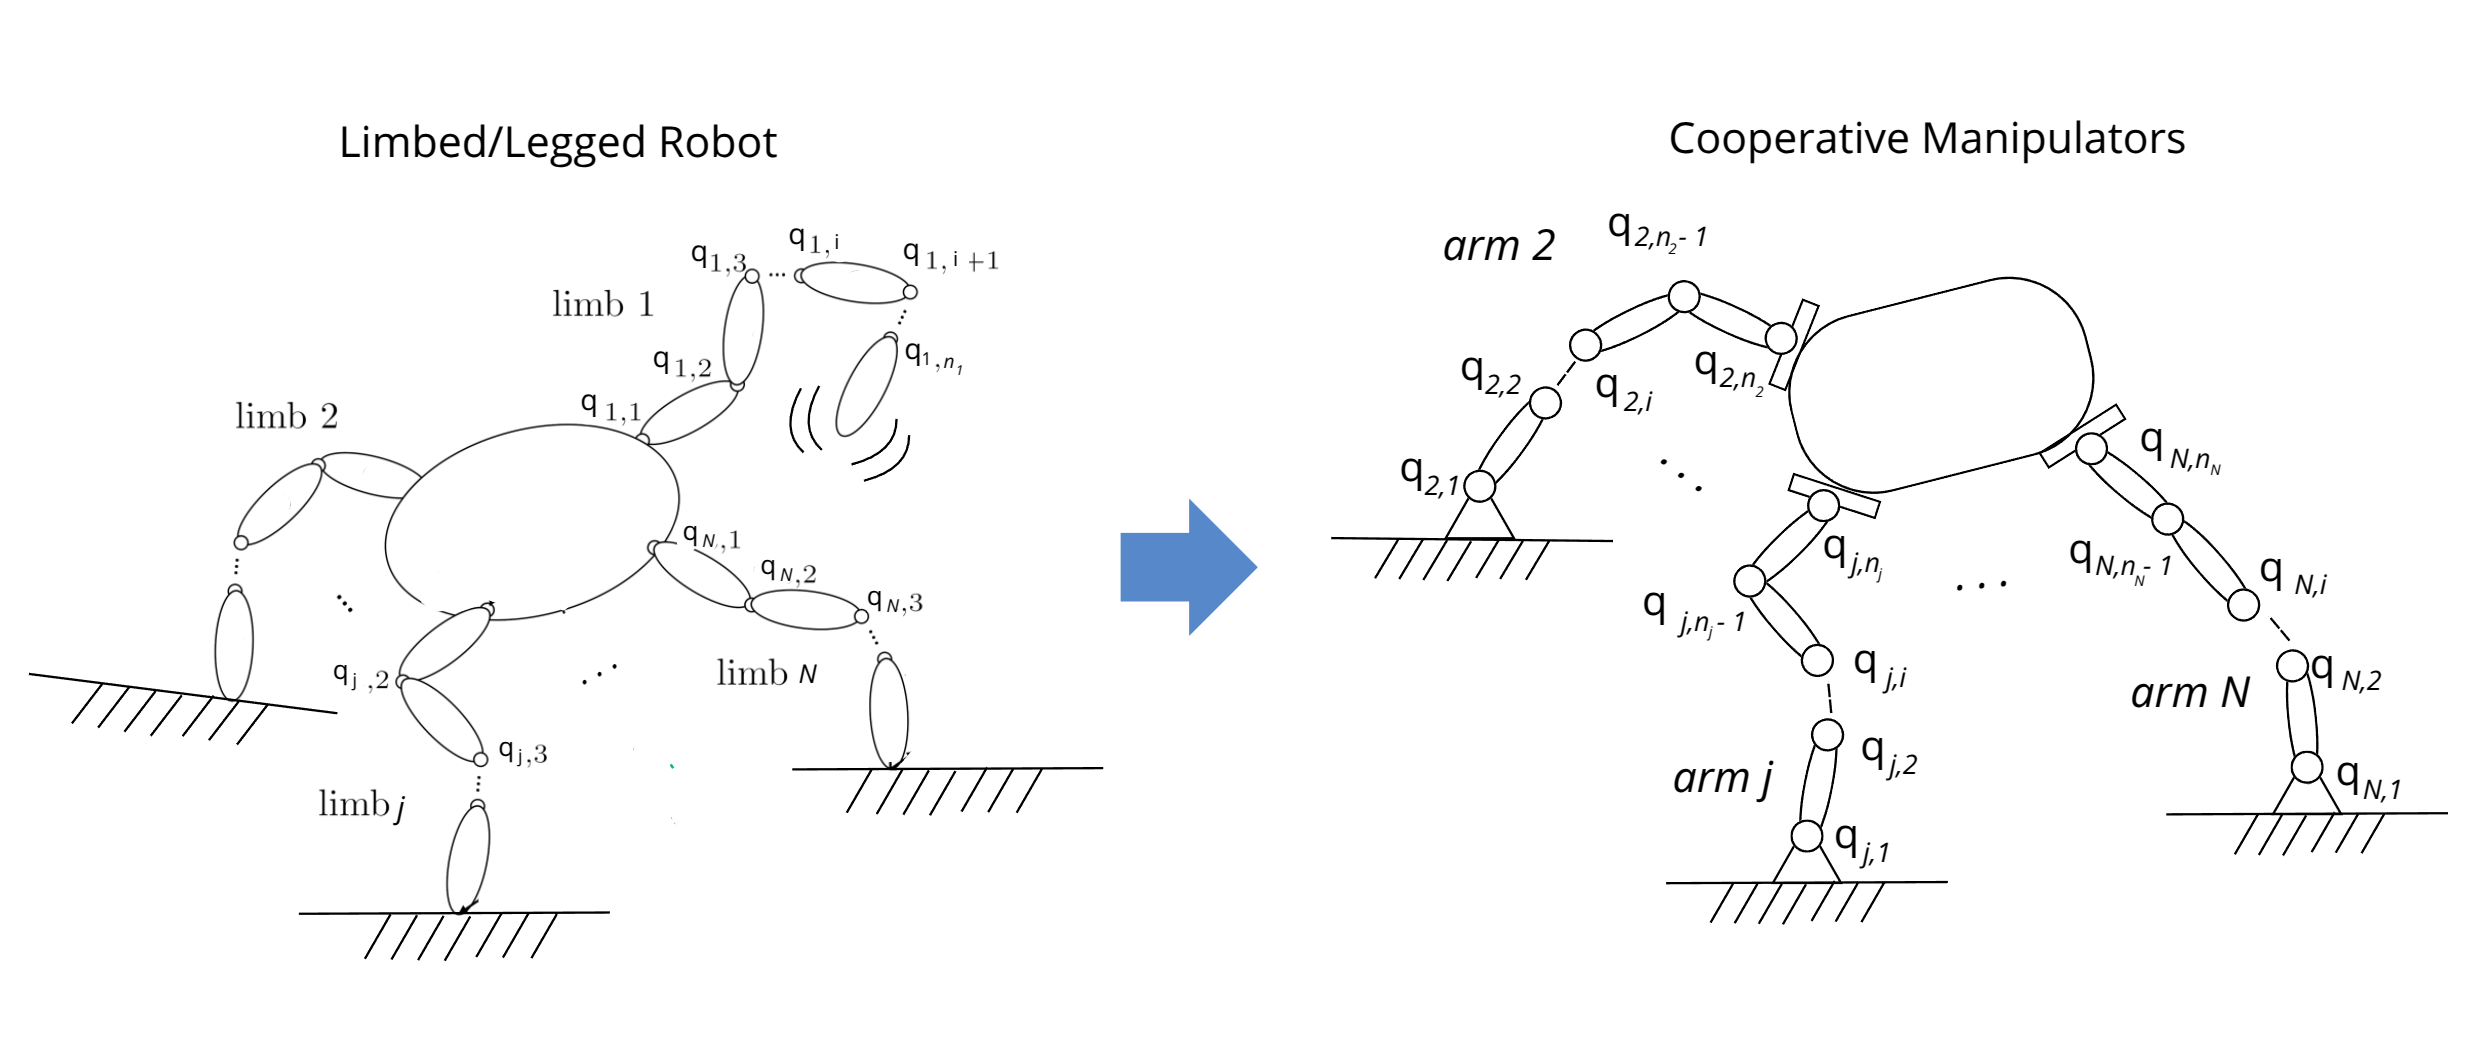
\includegraphics[width=1.0\textwidth]{Images/img_ch2/MultiArmLimbedParallel.png}
    \caption{Parallelism between limbed/legged robot and cooperative manipulator}
    \label{fig:MultiArmLimbed}
\end{figure}

The final relationship derived from this approach is again in the form: 
\begin{equation}
\label{eq:LeggedMultiArm}
 \mathbf{v_b} = \mathbf{{J}(q)}\cdot\mathbf{\dot{q}}
\end{equation}

\section{Dynamic Model}
\label{sec:dynamic}
Dynamics complete the modeling tools needed to analyze and understand the motion of a mechanical system. While kinematics forget about the cause of motion, 
the objective of \textbf{dynamics modeling} is to derive the relationship between joint actuator torques and the motion of the structure\cite{Siciliano}. 
The dynamics model is fundamental to derive the systems' equations of motion (EoM), then used for \textbf{simulation} and \textbf{design of control algorithms}.

To derive those equations, two methods exist: 
\begin{itemize}
    \item \textbf{Lagrange formulation}: Systematic approach, based on energetic quantities differentiation. 
    Defining the Lagrangian function as $\mathcal{L} = \mathcal{T} - \mathcal{U}$ (where $\mathcal{T}$ and $\mathcal{U}$ are respectively the kinematic and potential energy of the mechanical system) and $\mathbf{\xi}$  the vector of generalized force associated to the joint variables $\mathbf{q}$:
    \begin{equation}
    \label{eq:Lagrangian}
     \frac{d}{dt}\left(\frac{\partial\mathcal{L}}{\partial\mathbf{\dot{q}}}\right)^T -  \left(\frac{\partial\mathbf{\mathcal{L}}}{\partial\mathbf{q}}\right)^T= \mathbf{\xi}
    \end{equation}

    \item \textbf{Newton-Euler formulation}: based on a balance of forces and moments for rigid bodies.
    Recursive algorithms to solve dynamics are often based on this approach\cite{Siciliano}. 
\end{itemize}

The Lagrange formulation is the method employed here because it derives the EoM in a compact analytical form, convenient for control design.  
Furthermore, dynamics branches into two problems: 
\begin{itemize}
    \item \textbf{Direct Dynamics}:\\
    \textit{Given initial joint state and velocity $\mathbf{q}(t_0)$, $\mathbf{\dot{q}}(t_0)$, applied external generalized forces at final frame $\mathbf{h_e}(t)$ and joint torques $\mathbf{\tau}(t)$ for $t>t_0$, determine joint acceleration $\mathbf{\ddot{q}}(t)$ for $t>t_0$.}\\
    Once this problem is solved, from $\mathbf{\ddot{q}}(t)$, it is possible to integrate and obtain $\mathbf{\dot{q}}(t)$, $\mathbf{q}(t)$, and then from kinematics, describe the motion of the frame of interest. This is the procedure used to simulate motion.  
    \item \textbf{Inverse Dynamics}: \\
    \textit{Given the desired joint motion $\mathbf{\ddot{q}}(t)$, $\mathbf{\dot{q}}(t)$, $\mathbf{q}(t)$ and knowing the external external generalized forces at final frame  $\mathbf{h_e}(t)$, determine the joint torques $\mathbf{\tau}(t)$ to achieve that motion.}\\
    Algorithms to control the system can be derived from the solution to this problem\cite{SurveyQuadrupeds}.    
\end{itemize}

Next, a brief survey of the EoM derived from the dynamics of some robotic structures is presented.

\subsection{Manipulators and Single-Leg/Limb}
\label{sec:manipulatorDyn}
The theory on Manipulator robots is well-established, and a standard EoM in matrix form is derived with the Lagrange approach: 
\begin{equation}
    \label{eq:ManipulatorEoM}
    \mathbf{B}(\mathbf{q})\mathbf{\ddot{q}} + \mathbf{C}(\mathbf{q},\mathbf{\dot{q}})\mathbf{\dot{q}} + \mathbf{F_v\dot{q}} + \mathbf{F_{s}}sgn(\mathbf{\dot{q}})+ \mathbf{g}(\mathbf{q}) = \mathbf{\tau} - \mathbf{J}^T(\mathbf{q})\mathbf{h_e}
\end{equation}
Where the matrices have the following meaning: 
\begin{table}[H]
    \begin{tabular}{ll}
        ${\mathbf{B}(\mathbf{q})}$ & Inertia Matrix ($n \times n$, symmetric and positive definite).\\[2pt]
        ${\mathbf{C}(\mathbf{q}, \mathbf{\dot{q}})}$ & Coriolis and Centrifugal Matrix ($n \times n$).\\[2pt]
        $\mathbf{F_v}$ & Viscous friction matrix ($n \times n$, diagonal).\\[2pt]
        $\mathbf{F_s}$ & Static friction matrix ($n \times n$, diagonal), coulomb friction model.\\[2pt]
        $\mathbf{g}(\mathbf{q})$ & Gravitational torque vector ($n \times 1$).\\[2pt]
   \end{tabular}
\end{table}
The other symbols have the same meaning as discussed before. 
In particular, $\mathbf{J}^T(\mathbf{q})\mathbf{h_e}$ map the generalized force exerted by the EE to the joint space (similarly to the static relationship \ref{eq:Static}). When a generalized force $\mathbf{h_c}$ is applied at a generic point $\mathbf{C}$ in the structure, the mapping is straightforward, an additional contribution of $\mathbf{\tau_c} = \mathbf{J_c}^T(\mathbf{q})\mathbf{h_c}$ is subtracted at the left-hand side of the EoM \cite{DeLucaContact1}. 

The dynamic model above is highly coupled and configuration-dependent, for control purposes, a decoupled joint model can be derived. 

\subsubsection{Decoupled Model}
\label{sec:DecoupledDyn}
The joint space vector $\mathbf{q}$ used until now, refers to the change of position of the link from the initial one, neglecting what happens at the motor level. 
Gearboxes are usually used for joint actuation, a gearbox provides a mechanical transmission between the motor and load, with reference to Fig.\ref{fig:TransmissionMotor}, the following relationship holds: 
\begin{equation}
\label{eq:Transmission}
    \begin{cases}
        q_l = \frac{1}{N_{gear}}q_m \\
        \dot{q}_l = \frac{1}{N_{gear}}\dot{q}_m \\
        \mathbf{\tau}_{l} = N_{gear} \mathbf{\tau}_{lm} \\
    \end{cases}
\end{equation}
Where $N_{gear}$ is the transmission ratio (or gear ratio), $\tau_l$ the torque at the load side (corresponding to $\tau_i$, $i^{th}$ joint torque of $\mathbf{\tau}$),  $\tau_{lm}$ the load torque transferred at motor side, $\tau_{m}$ the motor torque, $J_m$ the motor inertia, and $J_l$ the load inertia.
Neglecting the friction effect, the motor dynamics is defined by the following equation: 
\begin{equation}
\label{eq:Transmission}
        J_{m}\ddot{q}_m = \tau_m - \frac{\tau_l}{N_{gear}} 
\end{equation}

\begin{figure}[H]
    \centering
    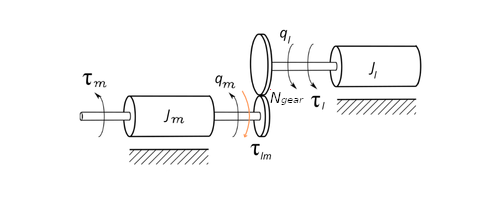
\includegraphics[width=1.0\textwidth]{Images/img_ch2/TransmissionMotor.png}
    \caption{\cite{Siciliano} Schematic representation of mechanical gear }
    \label{fig:TransmissionMotor}
\end{figure}

Considering a single row of the dynamic equation of the manipulator (neglecting external forces and friction), the load torque for the $i^{th}$ motor-transmission-load system is:
\begin{equation*}
    \label{eq:ManipulatorJointEoM}
    \tau_i = \mathbf{B_i}^T(\mathbf{q})\mathbf{\ddot{q}} + \frac{1}{2}\mathbf{\dot{q}}^T\mathbf{C_i}(\mathbf{q})\mathbf{\dot{q}} + g_i(\mathbf{q}) 
\end{equation*}
Then, collecting as residual the effect of Coriolis and centrifugal forces, gravitational load, and other joints ($j \not{=} i$) inertial effect: 
\begin{equation*}
    \label{eq:ResidualManipulator}
    \tau_{di} = \sum_{j\not{=}i}{C_{ij}(\mathbf{q})\cdot\dot{q}^2_j} +\sum_{j\not{=}i}{B_{ij}(\mathbf{q})\cdot\ddot{q}_j} + g_i(\mathbf{q})
\end{equation*}
And approximating $B_{ii}(\mathbf{q})$, representing the effect of inertia of joint $i$ due to its acceleration, as $B_{ii}(\mathbf{q}) \simeq \overline{B_{ii}} = J_{li}$ (as an average value over frequent joint configurations), the equation for $i^{th}$ joint become: 
\begin{equation*}
    \label{eq:TauJoint}
    \tau_i = J_{li}\ddot{q}_i + \tau_{di}
\end{equation*}
Introducing this load torque in Eq.\ref{eq:Transmission}, the resulting decoupled model, represented in Fig.\ref{fig:ManipulatorDecoupled} is: 
\begin{equation}
    \label{eq:DecoupledManipulatorEoM}
    \left ( J_{mi} + \frac{J_{li}}{N_{gear,i}^2}\right )\ddot{q}_{mi} = \tau_{mi} - \frac{\tau_{di}}{N_{gear,i}} \quad i = 1,\dots,n
\end{equation}

It is important to notice that the residual term $\tau_{di}$ is scaled up by $N_{gear,i}$, meaning that, high reduction ratios reduce the coupling effects, making the independent joint model a more accurate approximation. 
\begin{figure}[H]
    \centering
    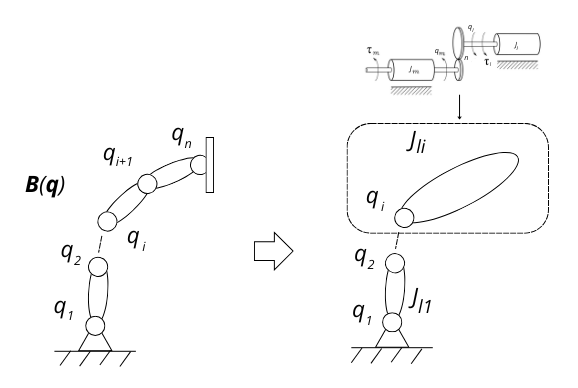
\includegraphics[width=0.75\textwidth]{Images/img_ch2/IJC.png}
    \caption{Schematic representation of decoupled manipulator model}
    \label{fig:ManipulatorDecoupled}
\end{figure}


Under the assumption that the base of a legged/limbed robot is static, the same equations describe a single leg/limb model from the root to the tip. 
In particular, this is useful in multipurpose multi-limb robots, when manipulation tasks are assigned, the EoM of the single limb can be considered as in Eq.\ref{eq:ManipulatorEoM} or Eq.\ref{eq:DecoupledManipulatorEoM}.

\subsection{Legged Robots, Walking Machines}
\label{sec:leggedDyn}

The mechanical complexity of walking robots and their intrinsic closed kinematic chain has been commented on several times. For this reason, forces and moments propagate from one leg to another, further increasing coupling effects. 
Considering the different approaches for walking robots discussed before, if a "stance-foot" modeling approach is used, the parallel manipulator model can be used, where only contact legs are considered. The dynamic model of parallel manipulator \cite{RoboticMechanics} with a minimal DOF as all leg joints can be derived. With this modeling approach, changing the stance foot causes a switch in the dynamic model, making the dynamics model a state machine with a number of states exponential in the number of legs.  
If instead a non-minimal number of DOF is used and the floating base DOFs model is employed, ( previously defined as: $\mathbf{q} = \begin{bmatrix}
    \mathbf{q_b} & \mathbf{q_1} & \mathbf{q_2} & \dots & \mathbf{q_N}
\end{bmatrix}^T$) it is possible to derive the EoM in a standard form with the Lagrange approach\cite{QuadrupedLocomotion}\cite{HandbookLegged} $\mathbf{q} \in \mathbb{R}^{n+6}, (n=\sum_jn_j)$: 
\begin{subequations}
    \label{eq:WalkingDyn}
    \begin{align}[left=\empheqlbrace]
           \mathbf{B}(\mathbf{q})\mathbf{\ddot{q}} + \mathbf{C}(\mathbf{q},\mathbf{\dot{q}})\mathbf{\dot{q}}+ \mathbf{g}(\mathbf{q}) = \mathbf{J_M}^T(\mathbf{q})\mathbf{\tau} - \mathbf{J_C}^T(\mathbf{q})\mathbf{h_c} \label{eq:WalkingEoM} \\
    \mathbf{J_c}\ddot{\mathbf{q}} + \mathbf{\dot{J}_c}\dot{\mathbf{q}} = 0\label{eq:walkingEoMConstraint} 
    \end{align}
\end{subequations}

Eq.\ref{eq:walkingEoMConstraint} represents the holonomic contact constraint of null velocity at contact point $\mathbf{v_c} = \mathbf{J_c}(\mathbf{q})\mathbf{\dot{q}} = \mathbf{0}$, and 
the matrices involved include the self and coupling effects of all leg joints and base DOF, so they have bigger dimensions than Eq.\ref{eq:ManipulatorEoM}. The matrix $\mathbf{J_M}$ maps all leg joint torques in the space of generalized coordinates.

Under some assumptions, the dynamics can be simplified\cite{Legged}\cite{HumanoidRobot}\cite{HandbookLegged}\cite{ModelingControlLegged}, providing a tool for the dynamical analysis of the robot, simple simulation, and controller design.  

For example, as described in \cite{ModelingControlLegged}\cite{Legged}\cite{ArticulatedRobots}, the non-actuated (virtual DOF of the base) part of the EoM can be rewritten as the Newton-Euler equation of the whole system: 
\begin{equation}
    \label{eq:CoMDynamicWalking}
    m(\ddot{\mathbf{c}} + \mathbf{g}) = \sum_i{f_i}
\end{equation}

Where $\mathbf{c}$ is the position of the whole robot CoM, $\mathbf{g}$ is the vector of gravity, and $f_i$ are the external forces. 
Equation \ref{eq:CoMDynamicWalking} doesn't provide details on the controlled DOFs, but it is important because it highlights that to generate any motion ($\ddot{c} \not= 0$) different from the gravitational falling effect, interaction forces $f_i$ are needed, so the goal of any motion algorithms will be to achieve a proper ground interaction.
Other models include the cart-table and the inverted pendulum\cite{Todd}.


\subsection{Limbed Robots, Multipurpose Machines}
\label{sec:limbedDyn}
If modeling the dynamics of walking robots is complex, for multi-limbed multipurpose robots it is even harder. The main difference is in the interaction of each limb with the environment. In Eq.\ref{eq:WalkingEoM}, the external force $\mathbf{h_c}$ model ground interaction during walking locomotion, only as pushing force, usually modeled using contact model as the friction cone \cite{ModelingControlLegged}\cite{WBCFocchi}. For multi-limb robots instead, the interaction can include manipulation and so additional payload, climbing with pushing forces\cite{RibeiroGroundGripping}, and hybrid wheeled-legged locomotion\cite{AnymalDocThesis}. An equation similar to \ref{eq:WalkingEoM} can be derived, but the modeling of $\mathbf{h_c}$ becomes harder. 

\section{Motion Control, State of the Art}
\label{sec:motionControl}

The objective of motion control is to enable the system's autonomy, and two main approach are used in controlling robotics systems\cite{LeggedSurvey}\cite{InteligentControlMultiLegged}: 
\begin{itemize}
    \item \textbf{Model Based}: the control algorithm exploits the knowledge of kinematics or dynamics model to compute the control action.
    \item \textbf{Model Free}: novel emerging approach like Reinforcement Learning\cite{AnymalDocThesis}\cite{RL_overview}, where the system learns a policy to execute tasks in the best way. 
\end{itemize}

In robotics, model-based algorithms are intrinsically multi-layered, the problem can be generalized in the following steps: 
\begin{enumerate}
    \setlength\itemsep{-0.7em} 
    \item Definition of the task (high-level)
    \item Conversion of task into system DOFs (middle-level)
    \item Actuation of DOFs (low-level)
\end{enumerate}

Each level has more functions, and
the accuracy and reliability of control can be ensured only when the system state is continuously observed, implementing a \textbf{feedback} control strategy\cite{Siciliano}\cite{CorkeMATLAB}. 

This closed-loop control principle is defined as the "sense-plan-act" architecture (in Fig.\ref{fig:RobotControl}), composed of the main components to achieve autonomy:
\begin{itemize}
    \setlength\itemsep{-0.7em} 
    \item \textbf{sensors}: To perceive the internal state (proprioceptive) and the surroundings (exteroceptive)
    \item \textbf{actuators}: To effectively interact with the environment and perform actions.
    \item \textbf{controllers}: connect perception and action by a control logic, as the one defined above.  
\end{itemize}

\begin{figure}[H]
    \centering
    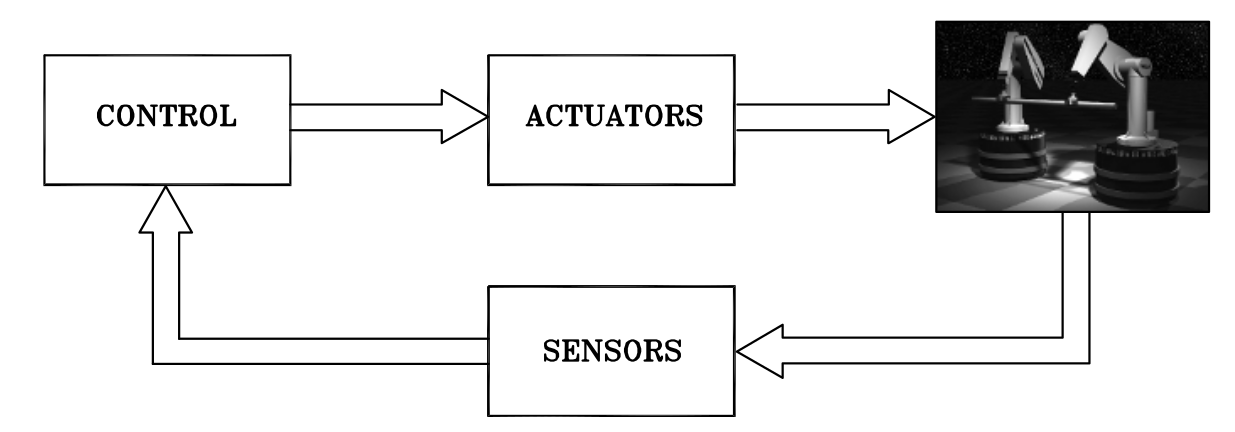
\includegraphics[width=0.7\textwidth]{Images/img_ch2/RobotControl.png}
    \caption{\cite{Siciliano} Closed loop sense-plan-act architecture}
    \label{fig:RobotControl}
\end{figure}

Next, the control architecture for manipulators is defined, then, legged and multi-limbed robots are discussed.  

\subsection{Manipulators}
\label{sec:manipulatorControl}

In manipulator robots, the desired task is defined by a sequence of the EE positions, to be reached autonomously without colliding with obstacles. The main functions of the control architecture layer, represented in Fig.\ref{fig:ManipulatorControlScheme}, are: 
\begin{itemize}
    \setlength\itemsep{-0.7em} 
    \item \textbf{High-Level}: Tasks are generated autonomously by intelligent decision algorithms or by an operator.
    \item \textbf{Middle-Level}:  After generating the trajectory between the initial state (computed with FK from joint feedback) and the final state in EE coordinates, tasks are converted in joint space by IK. Then a control algorithm is used to compute the actuator input from the joint state reference.  
    \item \textbf{Low-Level}: Closed loop control of actuator command, like the motor torque's proportional integral derivative (PID) feedback control. 
\end{itemize}

Additionally, \textbf{state estimator} algorithms are included to keep track of the internal state of the system from sensor feedback.

The high-level task generator can be operated manually, or with more intelligent algorithms ensuring a complete level of autonomy. 
For example, in pick and place tasks or in machining, feedback from cameras and other sensors is used to generate the sequence of operations once the general task has been defined\cite{CorkeMATLAB}. 

For the middle-level control layer, only the control in the joint space is described here, but working directly in the task space is possible with appropriate algorithms\cite{Siciliano}. 

There are different choices for the control algorithms in the \textbf{axis controller}, which is responsible for moving the joints in the desired position, in the \textbf{model based} context,  some of the most common are: 
\begin{itemize}
    \setlength\itemsep{-0.7em} 
    \item \textbf{Indipendent Joint Control} (IJC): Decentralized control, based on the decoupled model defined in Eq.\ref{eq:DecoupledManipulatorEoM}.
    \item \textbf{Inverse Dynamics} (ID): From the desired joint state, dynamics equation \ref{eq:ManipulatorEoM} is solved in $\mathbf{\tau}$. This approach requires an accurate estimation of dynamic model parameters, often hard to obtain. 
    \item \textbf{Adaptive}: Based on adaptive control theory. 
    \item \textbf{Model Predictive Control} (MPC): Find the best control input as an optimization problem using the system model. 
\end{itemize}

\begin{figure}[H]
    \centering
    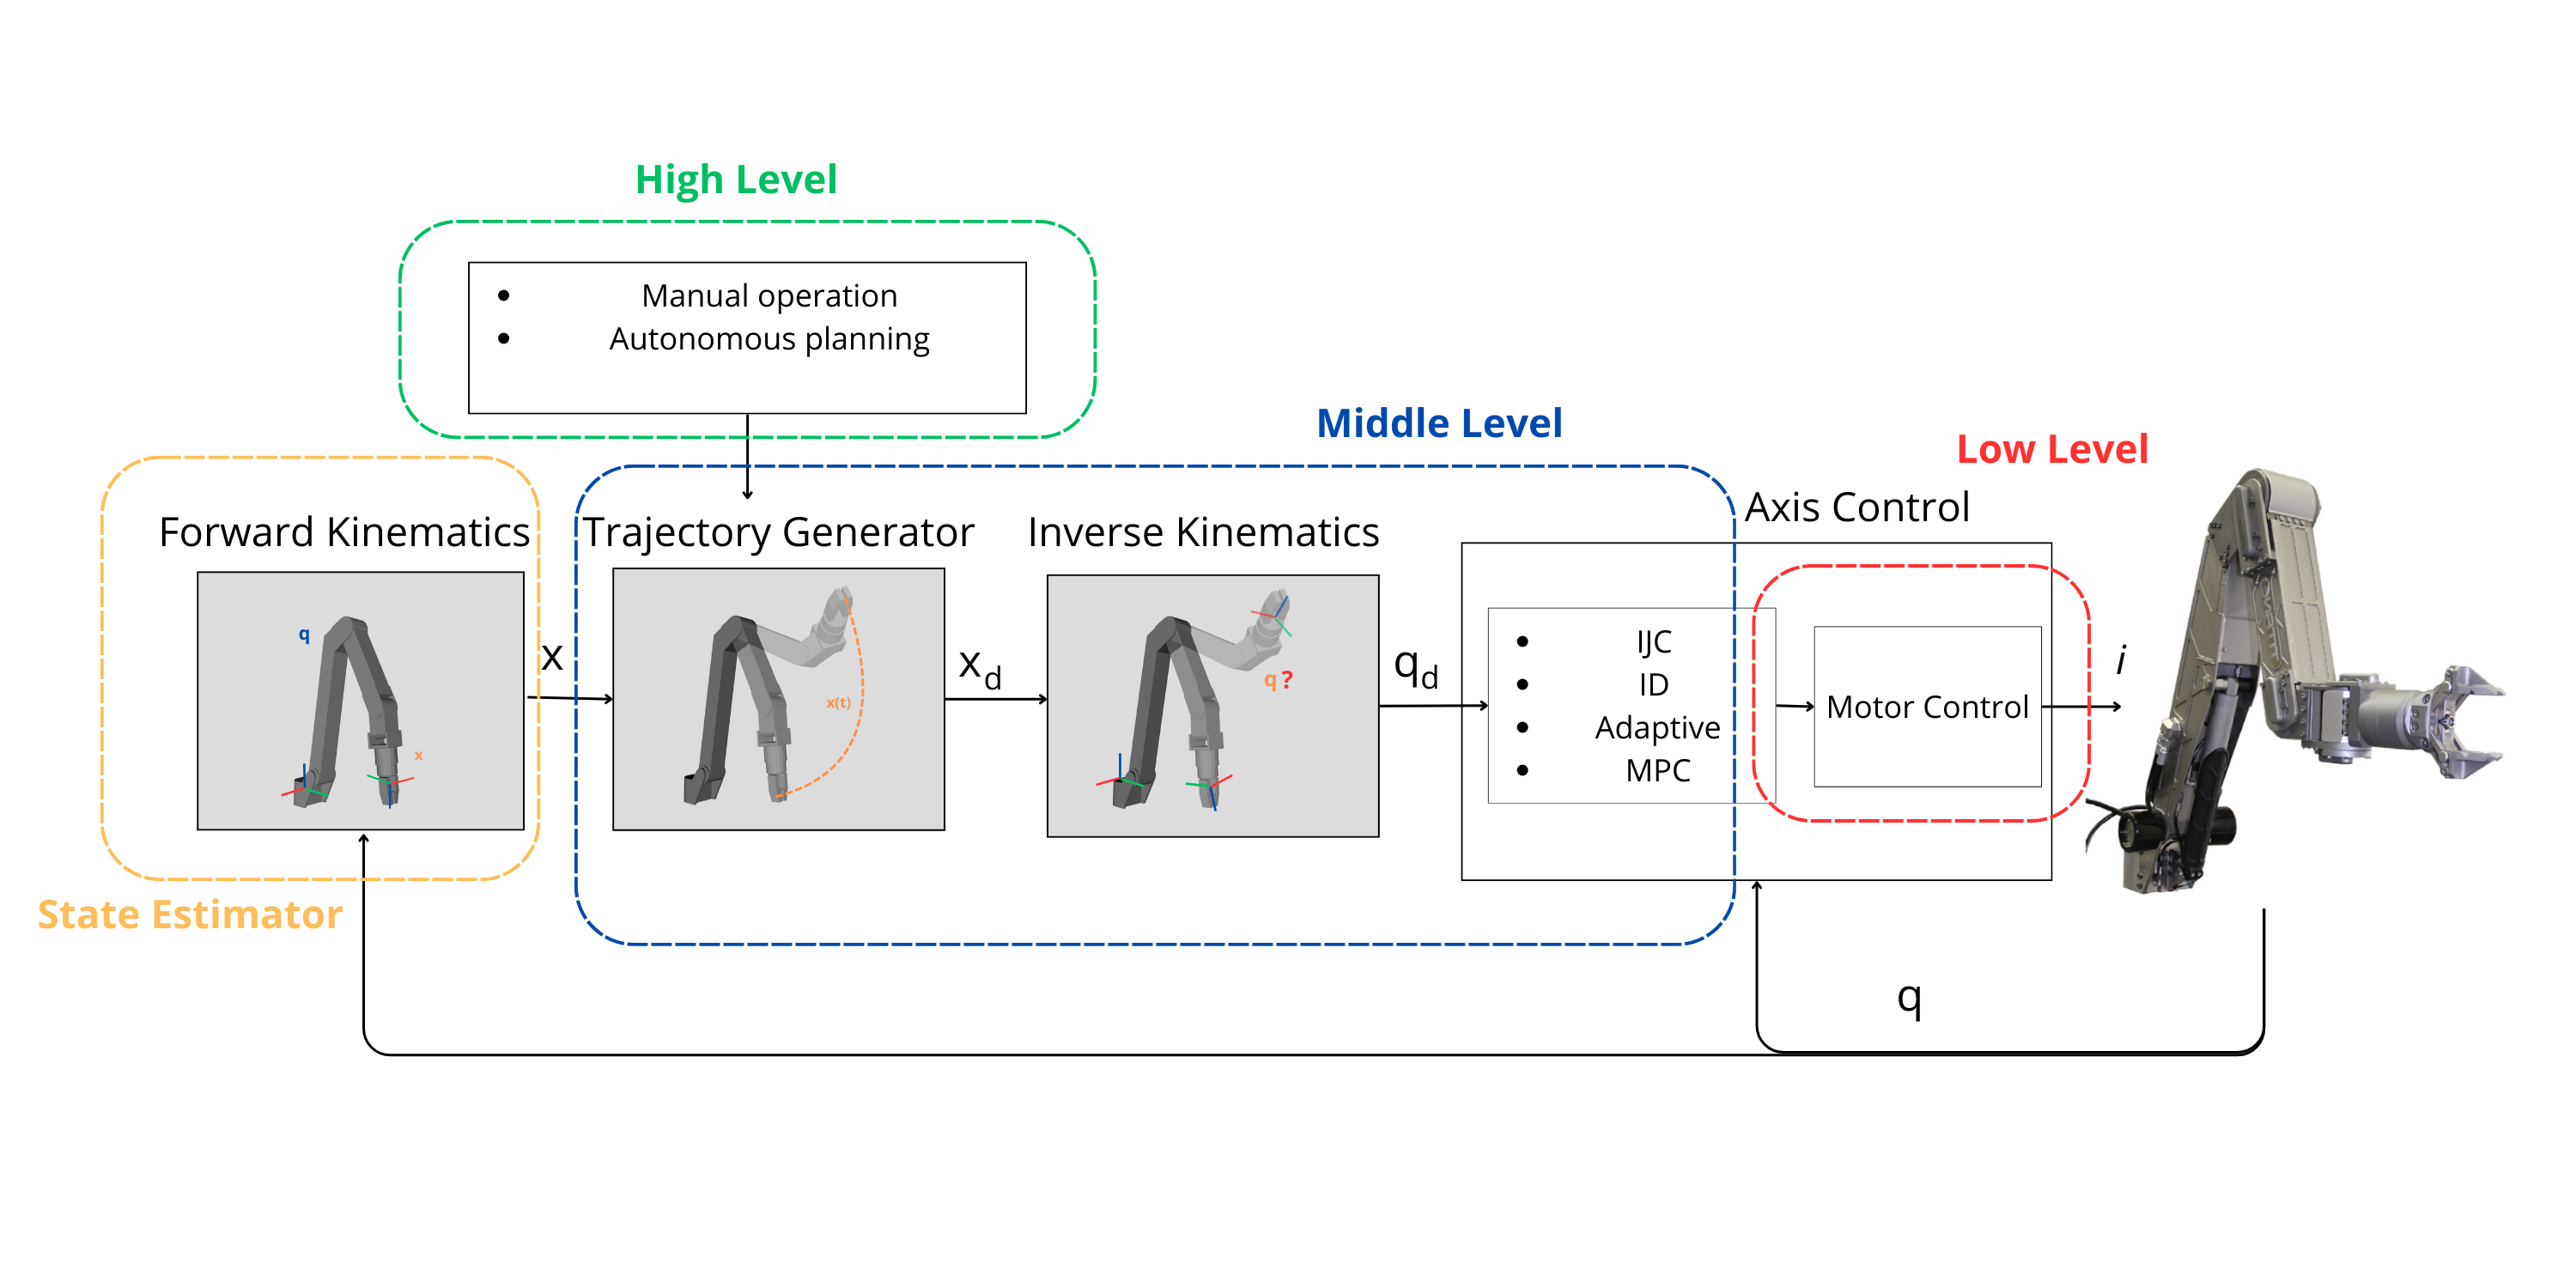
\includegraphics[width=1.1\textwidth]{Images/img_ch2/ManipulatorSchemeControl.png}
    \caption{Schematic representation of manipulator control architecture  }
    \label{fig:ManipulatorControlScheme}
\end{figure}

The IJC is a simple approach to controlling robot motion, for this reason, it is often used in robot prototypes. 

\newpage 
\subsubsection{Indipendent Joint Controller}
\label{sec:IndipendentJointControl}
The decoupled joint dynamics described by Eq.\ref{eq:DecoupledManipulatorEoM} is a good starting point for the design of a decentralized closed-loop control system of the whole robot.

In the Laplace domain, the transfer function from torque to position of each joint motor is:
\begin{equation}
    \label{eq:DecoupledManipulatorEoM}
    G_i(s) = \frac{q_{mi}(s)}{\tau_{mi}(s)} = \frac{\frac{1}{J_{mi} + \frac{J_{li}}{n_i^2}}}{s^2} \quad i = 1,\dots,n
\end{equation}

The idea behind a decentralized control structure is to control each subsystem (joint motor) independently from the others, as represented in Fig.\ref{fig:IJCScheme} below.

\begin{figure}[H]
    \centering
    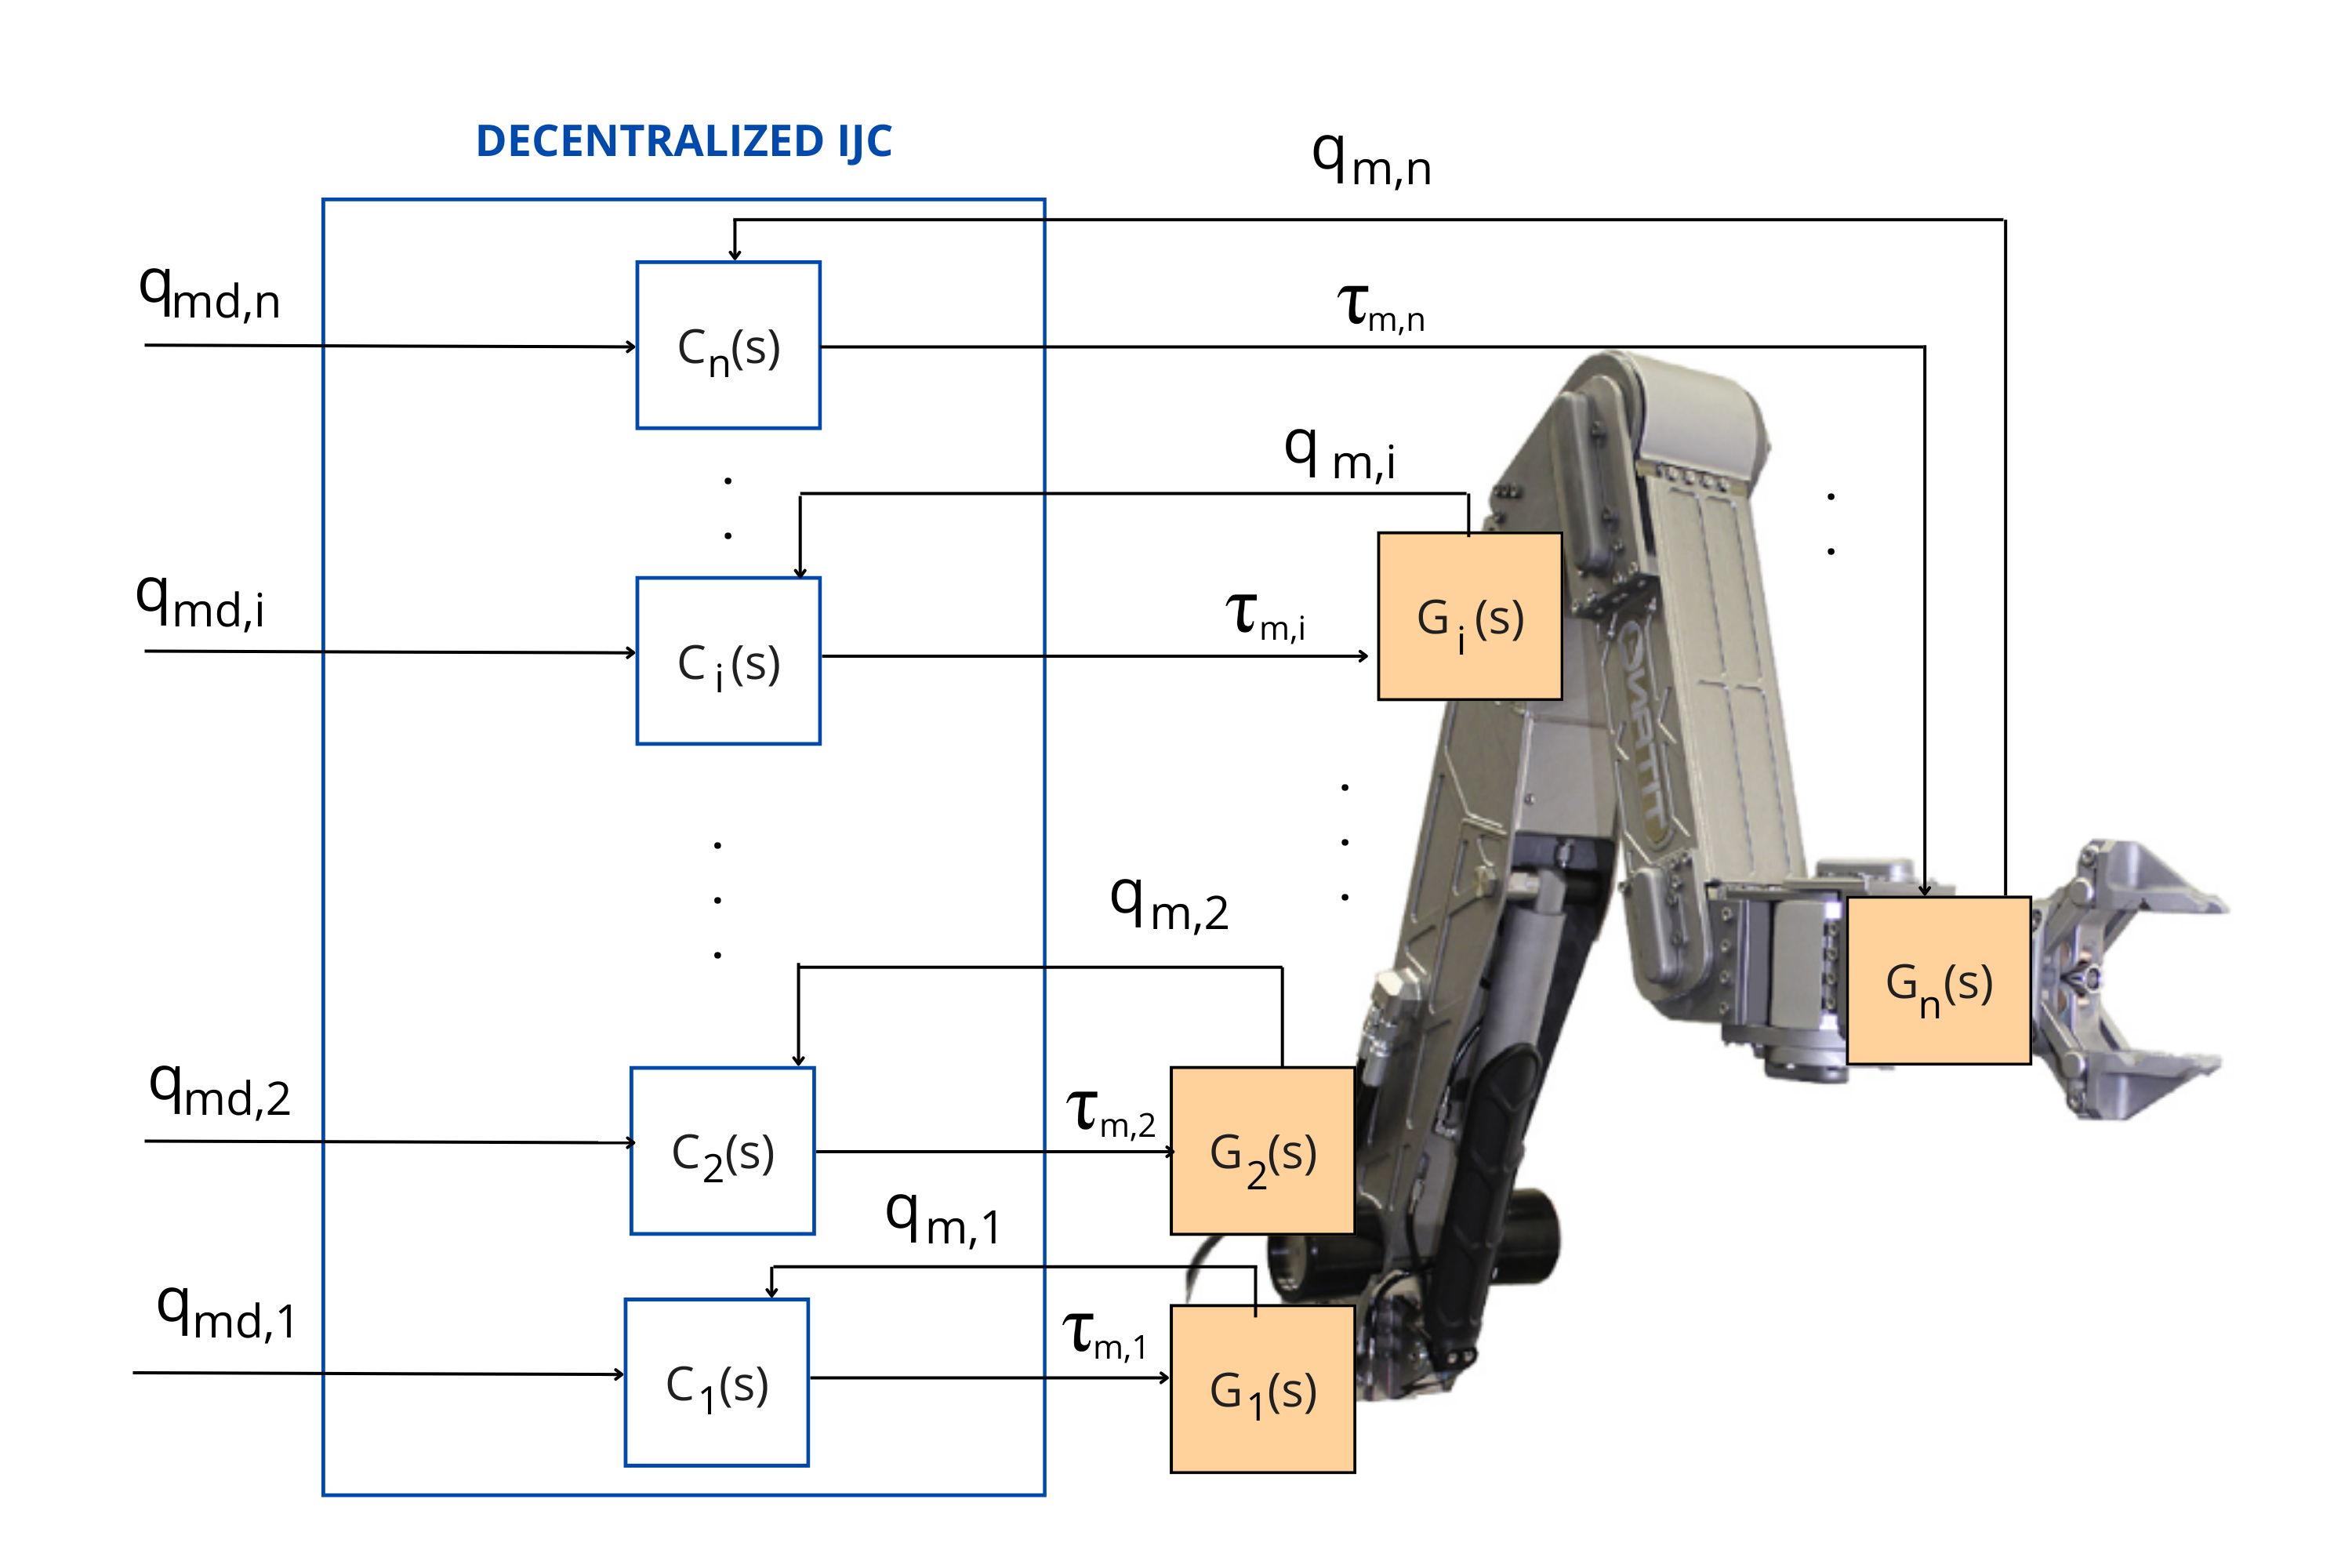
\includegraphics[width=0.7\textwidth]{Images/img_ch2/DecentralizedIJC.png}
    \caption{Schematic representation of a decentralized control structure for a manipulator}
    \label{fig:DecentralizedIJC_Arm}
\end{figure}


Fig.\ref{fig:PPI_IJC} represents the structure of each controller. The motor joint position is often controlled using a cascade controller structure(P+PI), with a proportional(P) in position controller and a proportional-integral(PI) in velocity, and a feed-forward velocity compensation, the controllers are properly tuned accordingly to the system requirements\cite{ControlTheory}.

\begin{figure}[H]
    \centering
    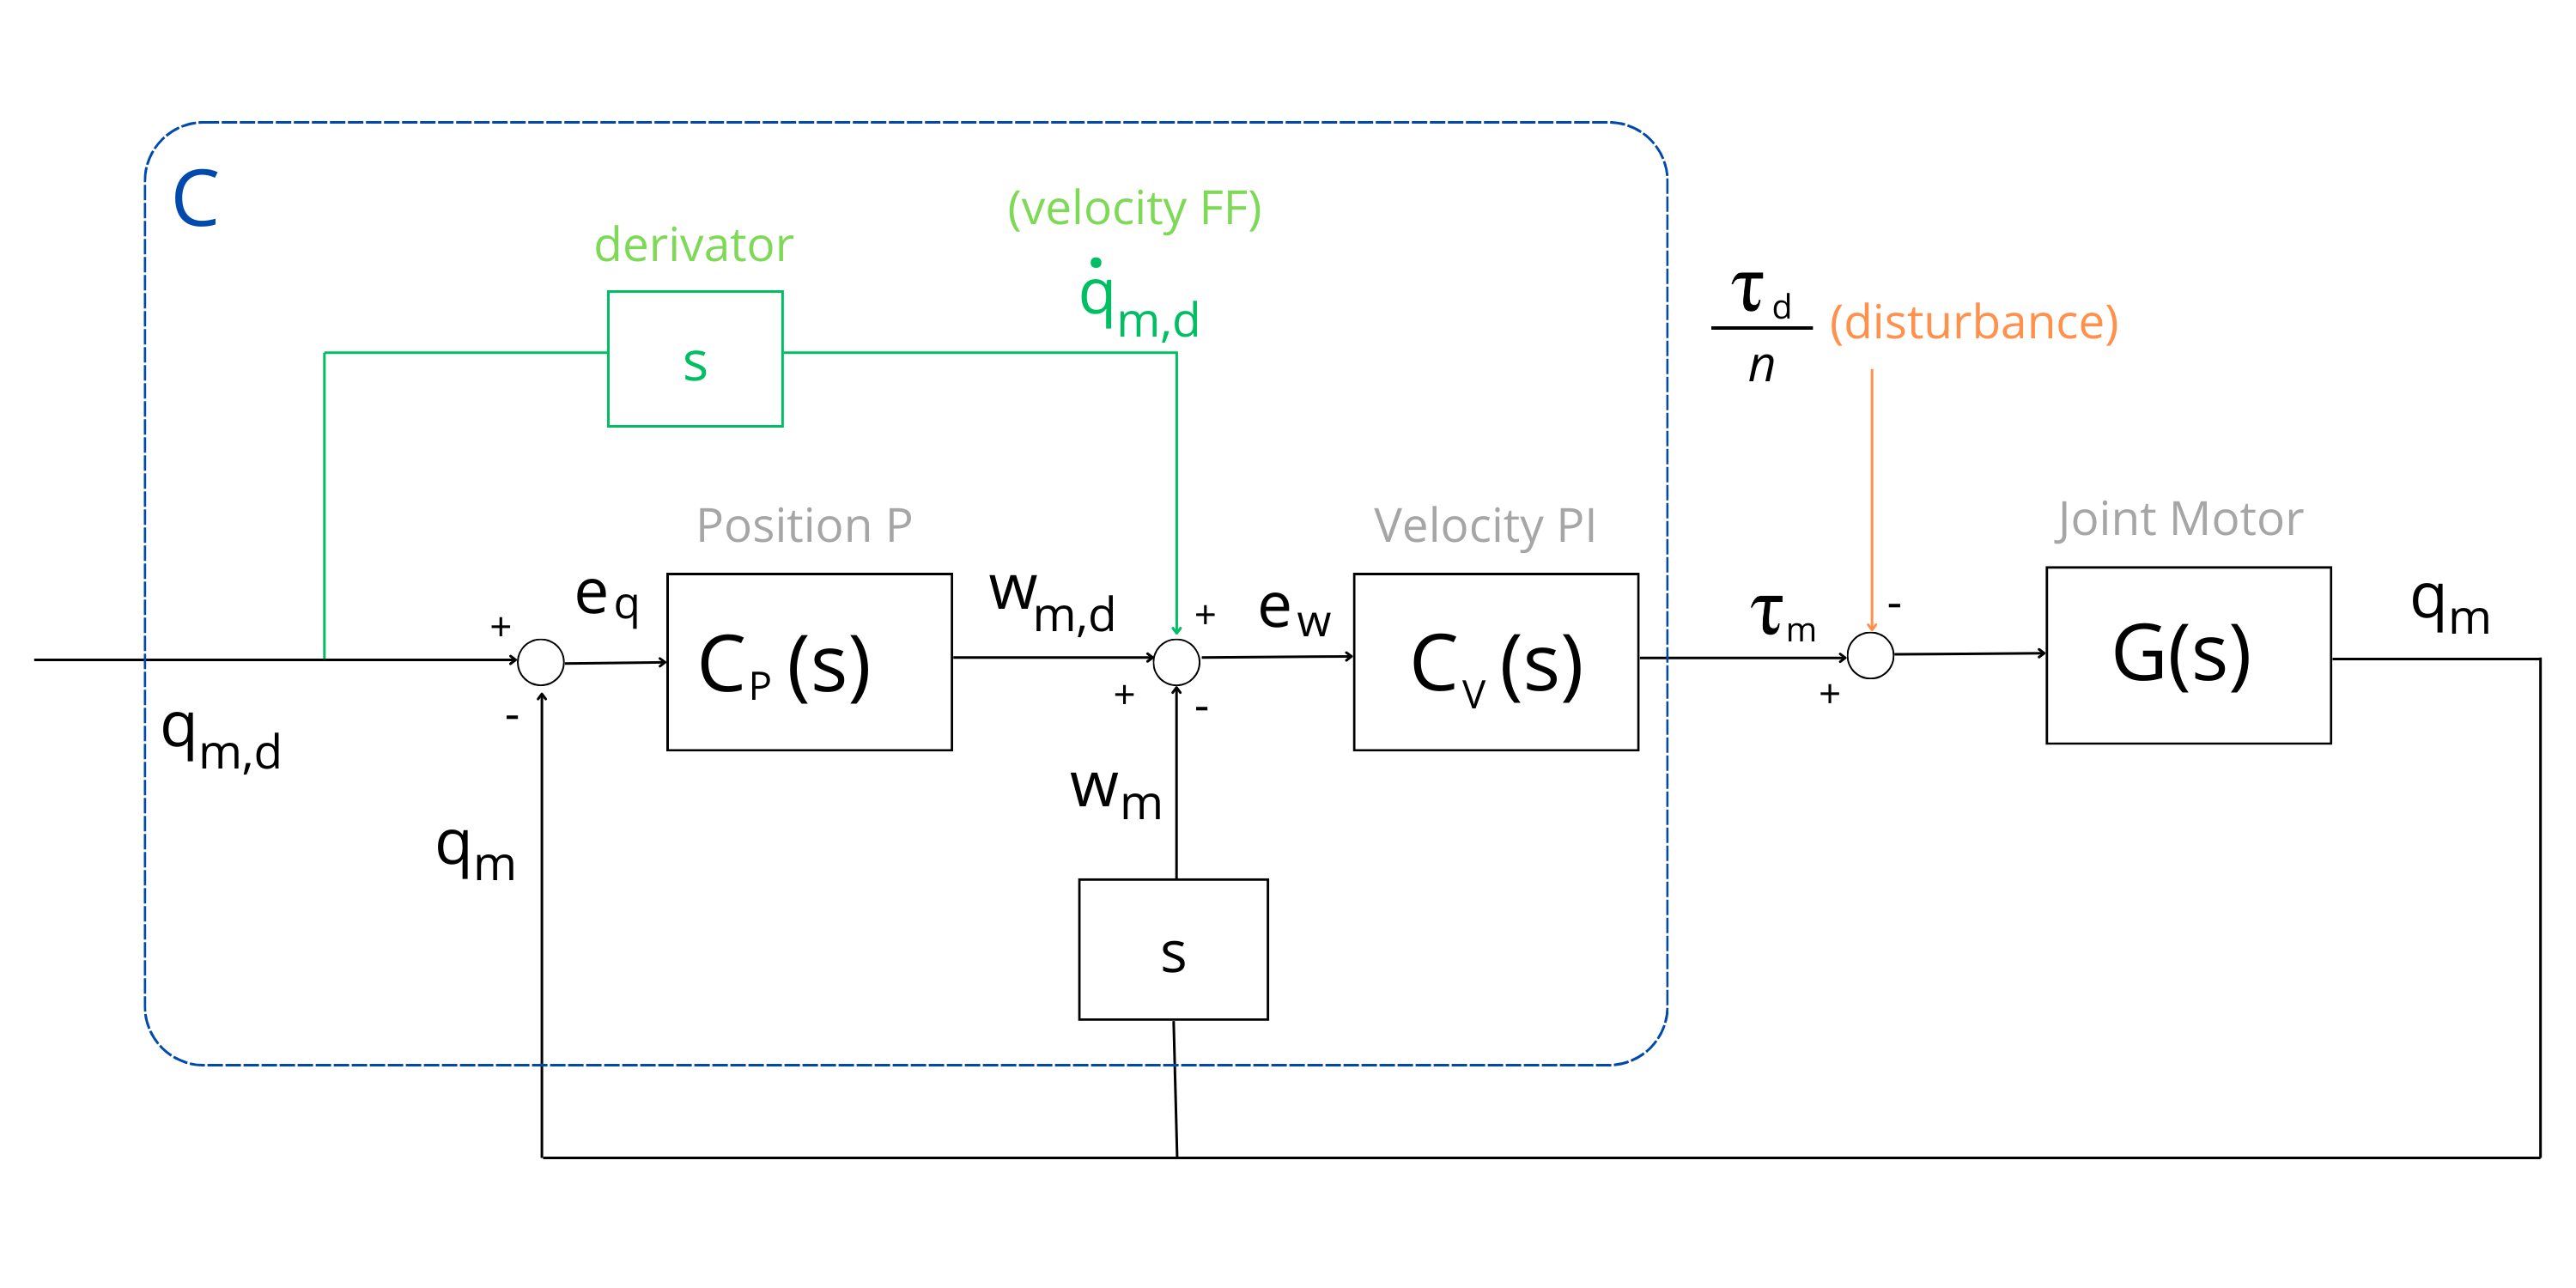
\includegraphics[width=0.7\textwidth]{Images/img_ch2/PPI_IJC.png}
    \caption{Block scheme of P+PI controller of each joint motor}
    \label{fig:PPI_IJC}
\end{figure}

Where the controllers have the following expressions in the Laplace domain: 

$C_P(s) = k_{pp}$ \quad $C_V(s) = k_{pv}\frac{1 + sT_{iv}}{sT_{iv}}$

\subsection{Legged Robots, Walking Machines}
\label{sec:leggedControl}

Legged robots introduce additional levels of complexity to the problem of motion control.
A set of base positions in space defines the motion task, to be executed with a chosen gait without falling or colliding with obstacles.
First of all, common for all mobile robots, the ability to move the base in the environment introduces a higher level of freedom, requiring a further ramification of control: 
\begin{itemize}
    \setlength\itemsep{-0.7em} 
    \item \textbf{Global planning/control}: long-term decision component, works with low frequency to define the trajectory from an initial point to a destination\cite{LeggedPlanning1}. This introduces the additional problem of understanding the environment through localization and mapping algorithms \cite{LeggedLocalization}\cite{AnymalDocThesis}.
    \item \textbf{Local planning/control}: ensure the execution of the global plan, working with high frequency. In legged robots, some of its main components are: gait scheduler, body trajectory control, and leg control (these elements are discussed in the next).  
\end{itemize}
In manipulators, the global planner is the high-level task generator, while the local planner is the architecture below that moves the robot.

Differently from wheeled robots, legged robots' motion is intrinsically discrete, with the advantage of higher traversability capabilities. 
But as introduced in chapter \ref{ch:chapter_one}, legs bring advantages but additional problems, such as base stability. Details on the techniques to evaluate stable conditions for the base position are discussed in chapter \ref{ch:chapter_three}. Intuitively, any legged system, including humans and animals, respects some configuration conditions to avoid falling, due to gravity and other inertial effect. For this reason, during motion, legs are positioned appropriately to maintain stability, humans and animals do it from a learning process, but machines must be instructed to do it. 

The definition of leg contact points along the trajectory is a complex task achieved by the global planner\cite{LIMBEROTakadaThesis}.
Leg order is decided by the \textbf{gait scheduler}, which generates a sequence of leg motion with a timing order, to move the base in a desired direction \cite{Todd}\cite{HiroseDesignGate}\cite{Raibert}. The \textbf{body trajectory controller} instead, keeps the body position in a stable configuration. 

The higher-level components of this architecture are out of the focus of this research, instead, the different techniques to control leg motion from the base specification are discussed now. 

\begin{itemize}
    \setlength\itemsep{-0.7em} 
    \item \textbf{Whole Body Controller} (WBC): Optimization-based control algorithm. Based on the desired base position and the dynamic model of the system, a constrained optimization problem is solved to compute the torque reference for all legs actuators \cite{AnymalDocThesis}\cite{WBCFocchi}\cite{WBCQuadruped}.
    \item \textbf{Model Predictive Control} (MPC): Similarly to the WBC this is an optimization-based control algorithms, which introduce the concept of receding horizon in its "Predictive" feature.  
    \item \textbf{Inverse Dynamic Torque-Based control} (IDC): Similarly to the ID control for manipulators, it is based on the ID problem for legged robots. From the Dynamic model inversion and the desired motion, the required joint torques are computed. When controlling motor torque, Impedance/Admittance control of legs is possible \cite{Siciliano}.
    \item \textbf{Inverse Kinematic Joint control} (IKJC): From the desired base motion, base IK is computed, obtaining each leg joint state. Then each leg is controlled with one of the techniques discussed for manipulator axis control (decentralized IJC, ID, Adaptive, MPC).
\end{itemize}

WBC, MPC, and IDC account for the whole robot dynamic model, ensuring better terrain adaptability, and performance, but dynamic model identification is usually hard.
In IKJC methods instead, each leg is controlled singularly, this is easy to implement but lacks terrain adaptability and ignores the coupled system dynamics. 

As for manipulators, this set of control problems requires a multi-layered control architecture, one possible control scheme is represented in fig.\ref{fig:LeggedControlScheme} below, respecting the "sense-plan-act philosophy". 
Including estimators for the state of the body, each leg, and the surroundings (map and terrain).

\begin{figure}[H]
    \centering
    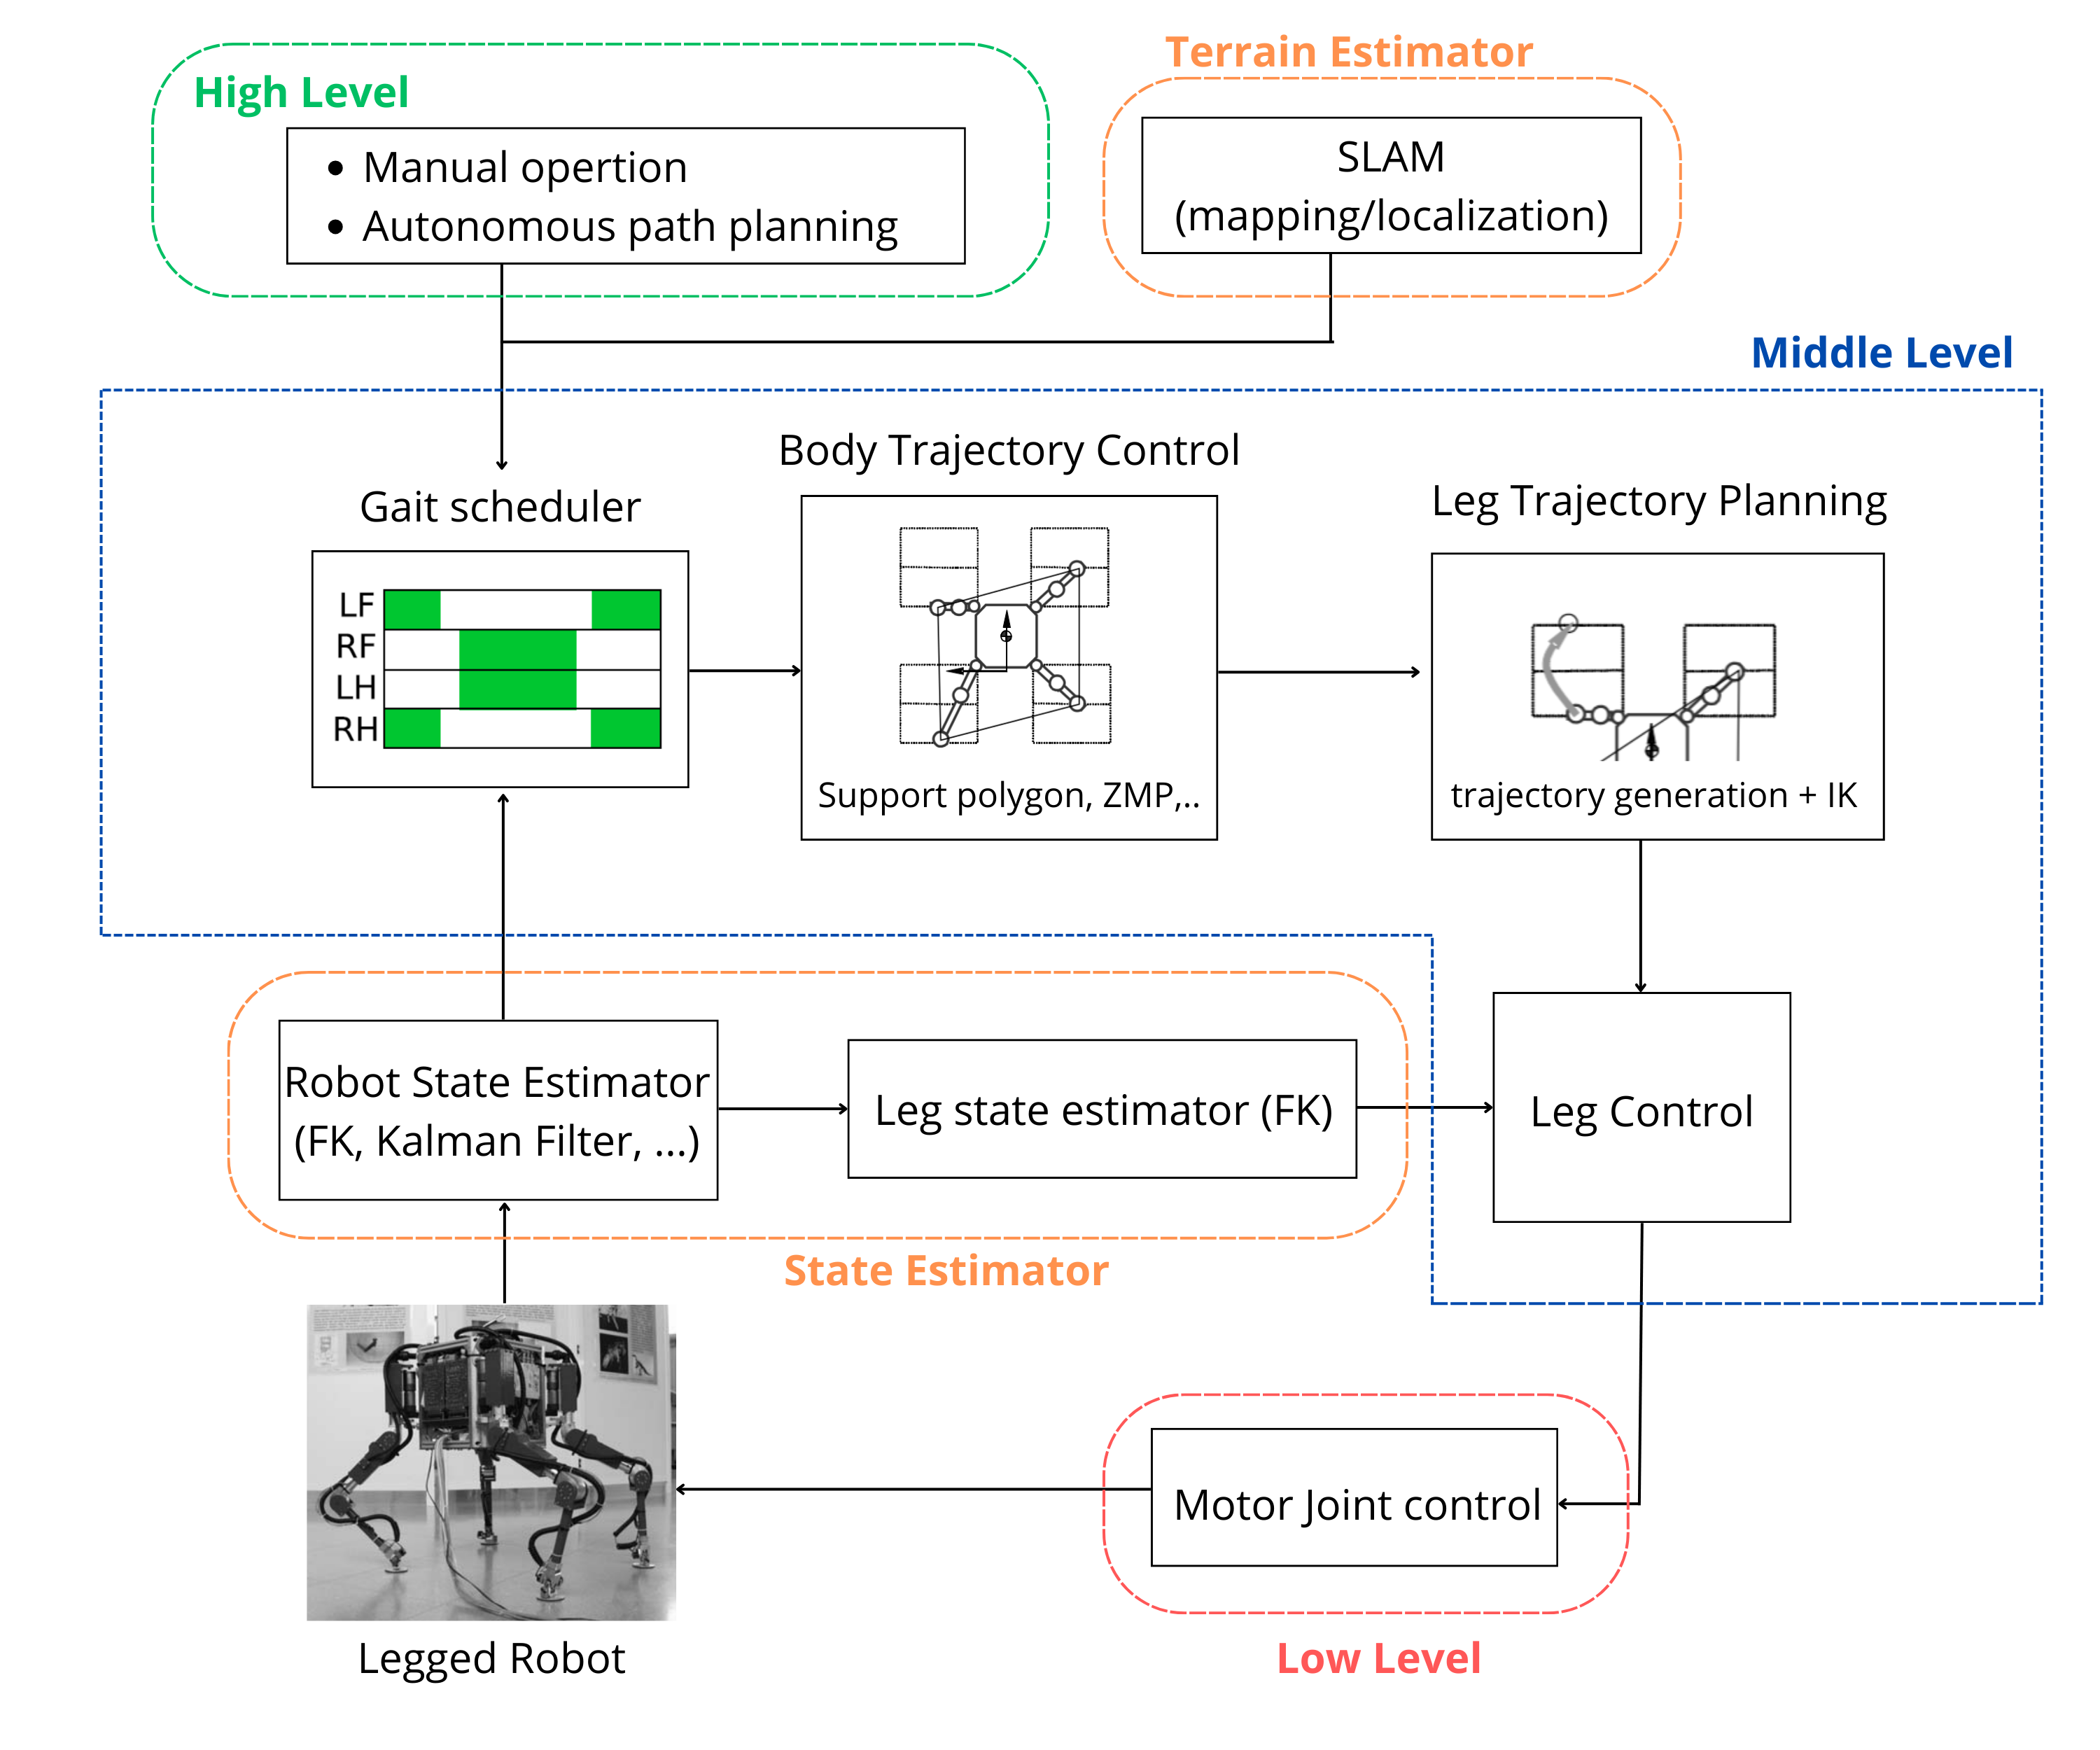
\includegraphics[width=0.8\textwidth]{Images/img_ch2/LeggedControlScheme.png}
    \caption{Schematic representation of one possible legged robot control architecture (some figures are taken from \cite{QuadrupedLocomotion})}
    \label{fig:LeggedControlScheme}
\end{figure}

\subsection{Limbed Robots, Multipurpose Machines}
\label{sec:limbedControl}
Defining a general control structure to control the motion of multi-limbed robots is not possible, due to their multipurpose nature. It is possible to give some task examples: 
\begin{itemize}
    \setlength\itemsep{-0.7em} 
    \item \textbf{Climbing robots}: the motion task is defined by a set of base positions in space (as for walking robot), to be reached while maintaining wall/ceiling adhesion and without colliding with obstacles\cite{KentaroUnoPhD}.
    \item \textbf{Walking/Climbing + Manipulating robots}: When limbs are designed also to manipulate objects in the environment. That means that tasks can be of two natures, reaching positions in space or moving limb tip in a sequence of positions, sometimes at the same time (walking while manipulating).
    \item \textbf{Driving + Walking robots}: legged-wheeled robots\cite{AnymalDocThesis}\cite{WheelLeggedStabilityOPT} add the additional legs DOF to the classical wheeled locomotion, making possible hybrid locomotion (like skating). The task is reaching poses in space, but additional decisional problems arise. 
    \item \textbf{Hybrid robots}: For robots equipped with transformable EE at limb tips, the complexity of modeling and control increases. Walking, climbing, driving, and manipulating tasks are unlocked. 
\end{itemize}

While walking machines are constrained to stay on the ground, space multi-limbed robots move around gripping the surroundings \cite{Ribeiro2023reaction}\cite{RibeiroGroundGripping}\cite{ISSLimbedRobot}. 
Professor Oussama Khatib implemented a possible solution to this complex scenario, the "constrained consistent task oriented WBC"\cite{KhatibConstrainedConsistentTaskOrientedWBC}. He defined a task-oriented control algorithm for humanoid robots, that can be generalized to different complex robotic structures.  
The details of this control algorithm are out of the scope of this research.

Another possible simpler solution is to consider again a multi-layered control structure, similar to the one discussed for walking machines (see Fig.\ref{fig:LeggedControlScheme}). In this case, additional complexity is included at a high level, where different types of tasks are generated. 
The output of high-level components will also include the type of task, and at middle-level decisions are taken accordingly. For the limb controller, reliable control algorithms (MPC, WBC, ID) are used to adapt to different tasks, such as moving the base, manipulating a heavy object, or gripping a rocky wall. 
Each module can be implemented using the concepts discussed for manipulators and climbing robots, but care must be taken due to the different tasks and situations addressed by the robot. 


\BlankPageTLGWone

\chapter{Stability and Performance Indices for Limbed Robots}
\label{ch:chapter_three}%

It is known that evolution has led living things to efficient anatomical structures: bipedal, quadrupedal\cite{bipedalVSquadrupedal}, hexapod, and octopods, 
this symmetry is not casual, and roboticists take inspiration from that\cite{robotsymmetry}.
An even number of legs allows the execution of periodic gaits and efficient locomotion\cite{LeggedSurvey}, and locomotion stability is guaranteed by repositioning the torso based on the position of the feet.
Stability is important whenever discrete, time-varying ground contact is involved, and understanding how to evaluate it is fundamental to designing and controlling any limbed or legged robot. Furthermore, legged locomotion is energy-expensive, and analyzing the performance and efficiency provides important insight.   

For the reasons above, this chapter presents tools for analyzing multi-limbed robots' stability and performance. Most of the theory discussed here was introduced for robots walking on legs but the same holds for limbed locomotion. 

First, quantitative state-of-the-art tools to evaluate system stability against falling are discussed. Then, performance in terms of efficiency is considered, introducing energetic indices related to power consumption during motion. 
Finally, a novel index to evaluate pose dexterity is formulated as an extension of the manipulability index for cooperative manipulators. This measure provides a visual tool to understand the motion capability of a robot in a given configuration, a problem not addressed until now. 

\section{Stability Indices}
\label{sec:stability_indices}
The challenge of achieving locomotion using legs has been studied long before the development of legged robots\cite{animalsInMotion}\cite{InsectLeggedWalking},
and McGhee and Frank have been the pioneers in the application of biomechanics on the legged mechanism\cite{LocomotionLeggedStudy}\cite{McGhee}\cite{Frank1968}.
They formalize the main theory behind legged robots, which is still used to study and characterize stability and gaits. First, some of their definitions are presented and reformulated, then from the limitations of those methods, other criteria are defined. 

\subsection{Static Stability}
\label{sec:static_stability}

Simplifying the leg tip as a single point, and defining the \textbf{contact points} as the position in the supporting plane where stance feet are located, the \textbf{support pattern} is defined as: 
\begin{definition}\label{def:support_pattern}
\cite{McGhee}The \textbf{support pattern} (or \textbf{support polygon}) is the minimum area convex point set in the support plane such that all of the leg contact points are contained 
\end{definition}
In simple terms, it is the area inside of the perimeter obtained by connecting the contact legs in sequence, as represented in Fig.\ref{fig:supportPolygon}.
\begin{figure}[H]
    \centering
    \subfloat{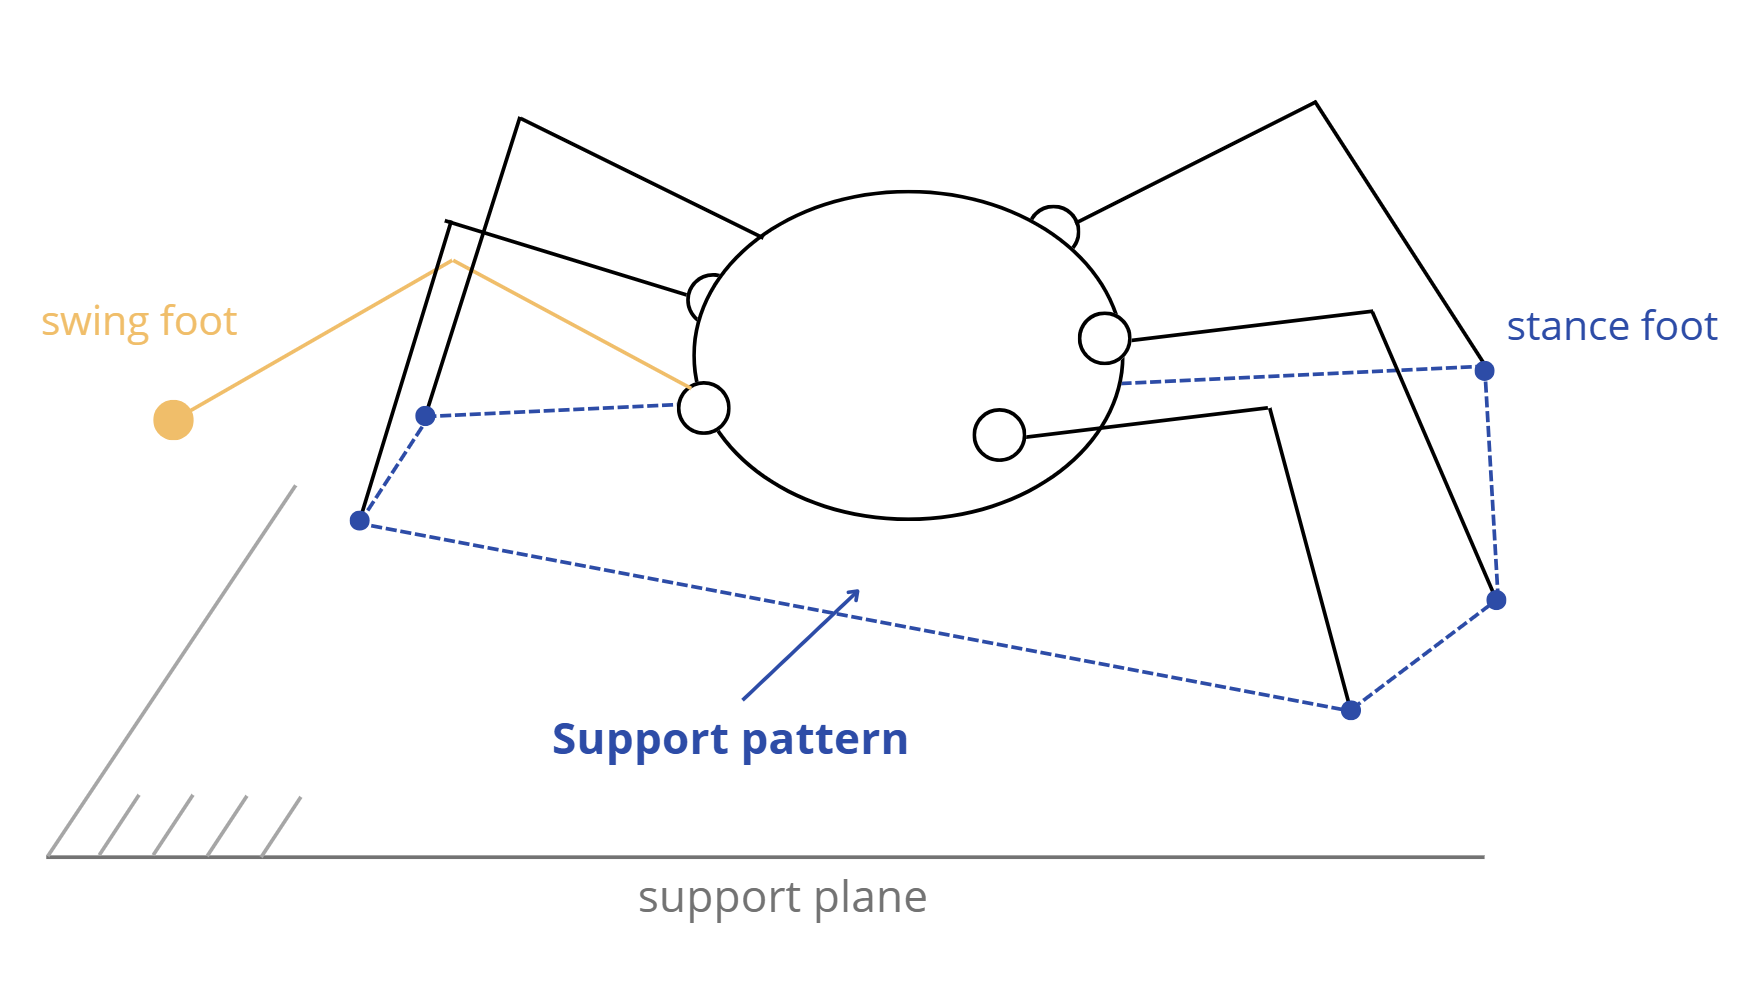
\includegraphics[scale=0.4]{Images/img_ch3/supportpattern1.png}}
    \subfloat{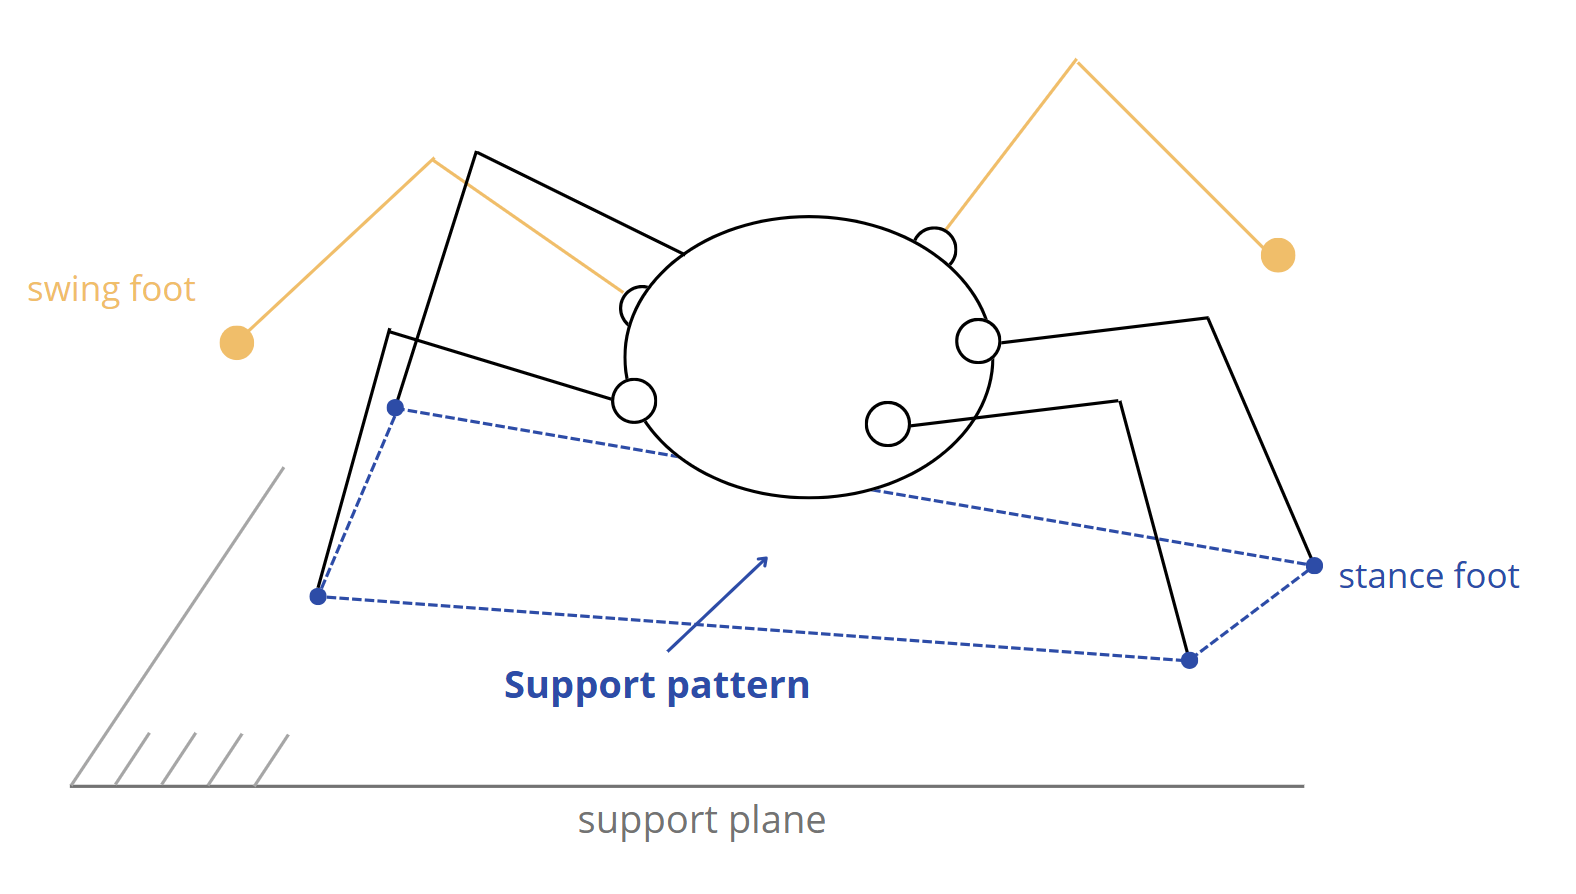
\includegraphics[scale=0.45]{Images/img_ch3/supportpattern2.png}}
    \caption[Examples of support pattern]{Example of support pattern in two different leg configurations.}
    \label{fig:supportPolygon}
\end{figure}

Support patterns are related to the static stability of legged machines, and a theorem to evaluate this stability for a horizontal support plane has been formalized \cite{McGhee}
\begin{definition}\label{def:static_stability}
A legged locomotion machine is \textbf{statically stable} at time $t$ if all legs in contact with the support plane at the given time remain in contact with that plane when all legs of the machine are fixed at their locations at time $t$ and the translational and rotational velocities of the resulting rigid body are simultaneously reduced to zero
\end{definition}
\begin{theorem}\label{th:static_stability}
A legged locomotion machine supported by a stationary horizontal plane surface is \textbf{statically stable} at time $t$ if and only if the vertical projection of the center of gravity of the machine onto the supporting surface lies within its support pattern at the given time
\end{theorem}

Theorem \ref{th:static_stability} holds for an ideal machine not subjected to external disturbances\cite{McGhee}, a notion of relative stability according to this theory is desirable to provide a margin of reliability.


\newpage
\begin{definition}\label{def:static_stability_margin}
\cite{McGhee}The magnitude of the \textbf{static stability margin}(SSM) at time $t$ for an arbitrary support pattern is equal to the shortest distance from the vertical projection of the center of gravity to any point on the boundary of the support pattern. If the pattern is statically stable, the stability margin is positive. Otherwise, it is negative.
\end{definition}

The SSM requires the computation of all the distances of the CoM projection from the support pattern perimeter, McGhee introduced an additional stability margin related to the direction of motion\cite{McGheeRoughLocomotion}:
\begin{definition}\label{def:static_stability_margin}
The magnitude of the \textbf{longitudinal stability margin} (LSM) at time $t$ for an arbitrary support pattern is equal to the shortest distance from the vertical projection of the center of gravity to the front or rear boundary of the support pattern as measured in the direction of travel 
\end{definition}

Using the kinematic model of multi-limbed robots introduced in \ref{sec:forward}, it is possible to reformulate these important concepts mathematically. 
The time dependency is neglected for notation conciseness, but all the quantities described are time-dependent, furthermore, all the 3D vectors above are measured in an inertial frame, for example, the World frame \textbf{w}. 
Remembering that the set of contact limbs has been defined as $J_c$, the support pattern (SP) is given by the convex hull formed by the contact points of the feet in the support plane $\mathbf{P}_{c,j},\forall j \in J_c$:

\begin{equation}
\label{eq:SP}
    SP = \text{Conv}(J_c) = \left\{ \sum_{j \in J_c} \lambda_j \mathbf{P}_{c.j} \;\Bigg|\; \sum_{j \in J_c} \lambda_j = 1, \; \lambda_j \geq 0, \; \forall j \in J_c \right\}
\end{equation}

Denoting with $\mathbf{P}_{CoM}$ the position of the base CoM, with $\mathbf{\overline{P}}_{CoM}$ its vertical projection on the support plane, theorem \ref{th:static_stability} can be reformulated. 
First, it is important to notice that the support plane is assumed horizontal, at height $z_0$ in the inertial frame, so $\mathbf{\overline{P}}_{CoM} = \begin{bmatrix} \overline{x}_{CoM} & \overline{y}_{CoM} & \overline{z}_{CoM}\end{bmatrix}^T \in \mathbb{R}^3$ can be reduced to a 2D vector $\mathbf{\overline{P}}_{CoM} = \begin{bmatrix} \overline{x}_{CoM} & \overline{y}_{CoM}\end{bmatrix}^T$ in the support plane, being $\overline{z}_{CoM} = z_0$ constant.  
This reduction of space allows to formulate the condition of static stability ($\overline{P_{CoM}} \in SP$) using the convex combination condition ($\overline{\mathbf{P}}_{CoM}$ is given by a convex combination of SP vertex, with the same formulation of SP points):
\begin{theorem}\label{th:static_stability_math}
A legged locomotion machine supported by a stationary horizontal plane surface is \textbf{statically stable} at time $t$ if and only if \\ $\exists \lambda_j \ge 0 \;,\; j\in J_c \;|\; \sum_{j \in J_c} \lambda_j = 1 \;, \overline{\mathbf{P}}_{CoM} = \sum_{j \in J_c} \lambda_j \mathbf{P}_{c.j}$
\end{theorem}

\newpage
Furthermore, with the same logic, it is possible to define a function $\sigma_{SS}(\overline{\mathbf{P}}_{CoM})$ equal to $+1$ if ($\overline{\mathbf{P}_{CoM}} \in SP$), $-1$ otherwise, this is needed to define the SSM correctly. 

\begin{equation}
\label{eq:sigma_SS}
\sigma_{SS}(\overline{\mathbf{P}}_{CoM}) = \
    \begin{cases}
    +1 \quad\text{ if } \exists \lambda_j \ge 0 \;,\; j\in J_c \;|\; \sum_{j \in J_c} \lambda_j = 1 \;, \overline{\mathbf{P}}_{CoM} = \sum_{j \in J_c} \lambda_j \mathbf{P}_{c.j}\\ \\ 
    -1 \quad\text{ otherwise}
    \end{cases}
\end{equation}

Finally, denoting with $\partial SP$ the perimeter of the SP, identified by all the edges $\overline{\mathbf{P}_{c.j}\mathbf{P}_{c.j+1}}\;,\; \forall j\in J_c$, the SSM can be defined as:
\begin{equation}
\label{eq:SSM_1}
    SSM = \sigma_{SS}(\overline{\mathbf{P}}_{CoM}) \cdot\min_{\mathbf{P}\in\partial SP}{\text{dist}(\overline{\mathbf{P}}_{CoM}, \mathbf{P})}
\end{equation}
Where dist($\mathbf{P_1}$,$\mathbf{P_2}$) denotes a measure of distance between $\mathbf{P_1}$ and $\mathbf{P_2}$, for example, the Euclidean distance in 3D space  $||\mathbf{P_2} - \mathbf{P_1}||$. 
This can be further reformulated considering that the SP perimeter is composed by the segments connecting the sequence of contact points: 
\begin{equation}
\label{eq:SSM_2}
    SSM =\sigma_{SS}(\overline{\mathbf{P}}_{CoM})\cdot \min_{j}{\frac{\left|(\mathbf{P}_{c,j+1} - \mathbf{P}_{c,j})  \times (\mathbf{P}_{c,j} - \mathbf{\overline{P}}_{CoM})\right|}{||\mathbf{P}_{c,j+1} - \mathbf{P}_{c,j}||}}
\end{equation}

Multiplying by $\sigma_{SS}(\overline{\mathbf{P}}_{CoM})$ is important to maintain the characteristic of the SSM to be positive is the legged robot is stable, negative otherwise. Clearly, the bigger the SSM and higher the level of stability, $SSM=0$ is a critical boundary condition, when $SSM < 0$ the robot is unstable.

To define the LSM, if the direction of motion is identified by the translational base velocity vector $\dot{\mathbf{p}}_b$, a mathematical formulation of that index requires also the identification of the intersection between the projection of the direction of motion in the support plane $\overline{\dot{\mathbf{p}}}_b$ and the support polygon perimeter $\partial SP$. This is not addressed here, instead Figure\ref{fig:SP_SSM_LSM} is a graphical representation of this, including the SP and the SSM.

\begin{figure}[H]
    \centering
    \subfloat[Stable configuration.\label{fig:stableLegged}]{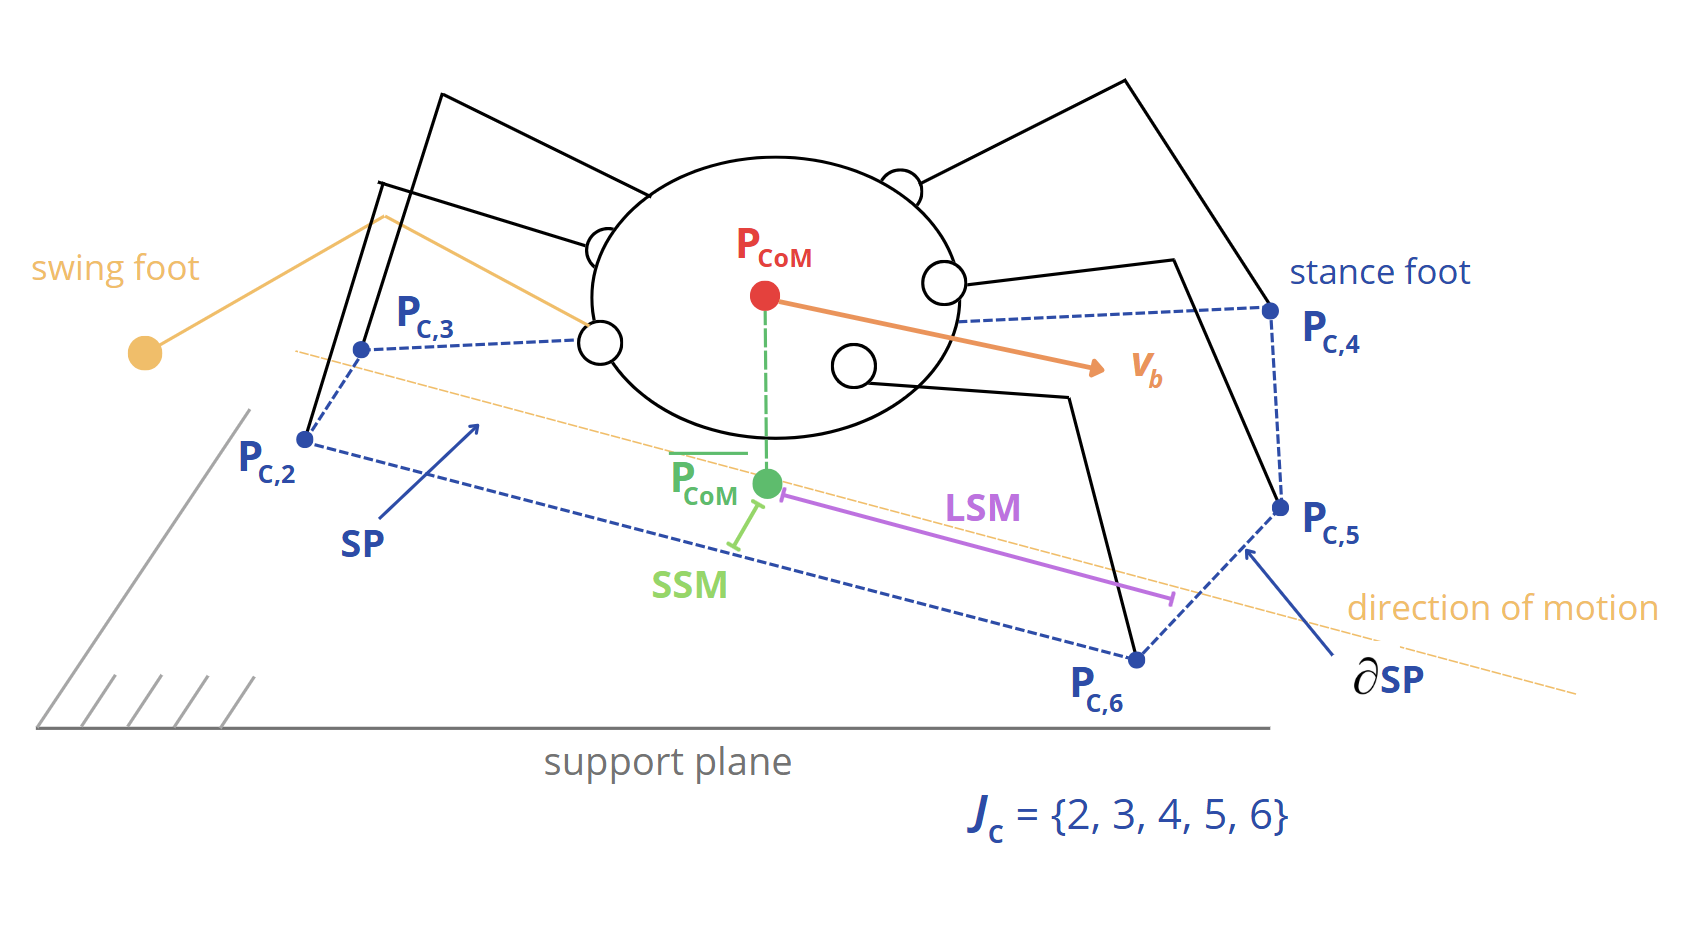
\includegraphics[scale=0.45]{Images/img_ch3/StabilityMargin1.png}}
    \subfloat[Unstable configuration.\label{fig:unstableLegged}]{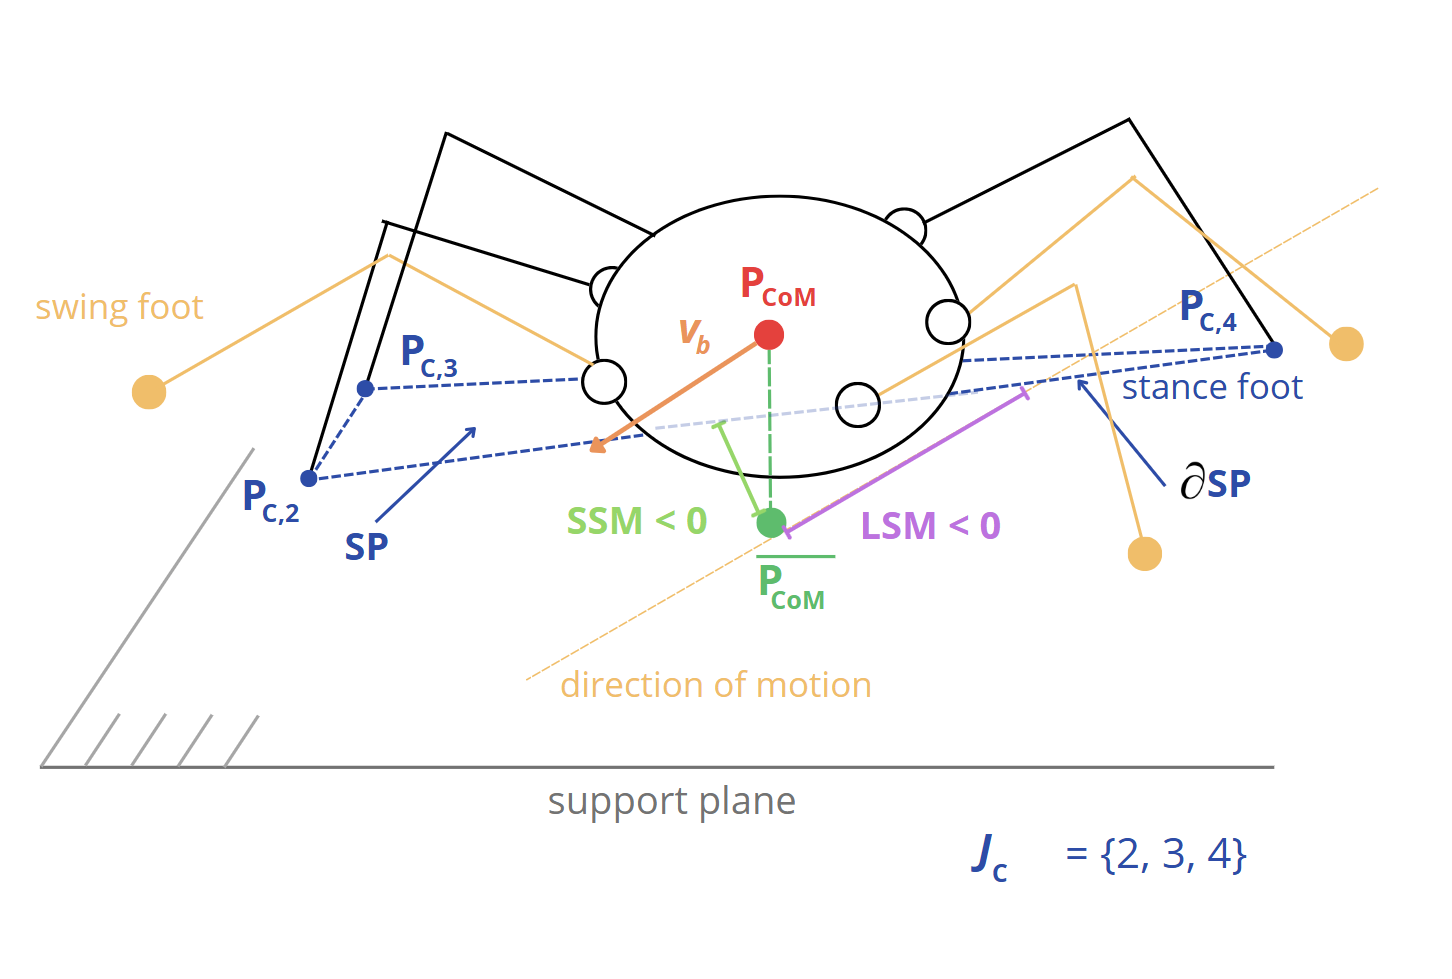
\includegraphics[scale=0.45]{Images/img_ch3/StabilityMargin2.png}}
    \caption[Examples of stability evaluation]{Example of statically stable and unstable robot configuration.}
    \label{fig:SP_SSM_LSM}
\end{figure}

As discussed in the previous chapter during the kinematic modeling of limbed robots, the base pose depends on all leg configuration $\mathbf{q} \in \mathbb{R}^n$, then $\mathbf{P}_{CoM}(\mathbf{q})$. This dependency is neglected in the notation, but it is important to remember that the robot is in a statically stable or unstable configuration depending on the leg joint state. 

This stability criteria, formalized from Equation \ref{eq:SP} to \ref{eq:SSM_2}, depends only on geometrical analysis and simple contact assumptions, and the validity is restricted when the support plane is horizontal (or at least approximately flat). Even if flat terrains of operation have been assumed for this research, it is relevant to give a brief overview of other methods that account for robot dynamics and interaction forces. 

\subsection{Dynamic Stability}
\label{sec:dynamic_stability}

One of the first studies on dynamic stability comes from the work of Vukobratović on anthropomorphic systems\cite{ZMP_vukobratovic}, which led to the definition of the zero moment point (ZMP). The ZMP is the point where the net moment of inertia force and gravity on the ground has no component in the horizontal direction\cite{ZMP_Vukobratovic_2}, and stability is maintained when it lays inside the SP. It has been widely used to evaluate both bipedal and multi-legged robot stability and gait generation \cite{ZMP_bipedal}\cite{ZMP_quadruped}\cite{ZMP_quadruped2}\cite{HandbookLegged}. It can be proven that when quasi-static motion is involved, ZMP and SSM stability criteria are equivalent\cite{HandbookLegged}.

Both the SSM and ZMP measure a stability margin as the distance of a point from the SP borders, the SP is a planar surface by definition. The limitation of the SSM is that that plane must be almost horizontal, while the ZMP, which considers gravity and inertial effect, is reliable also for slopes. In both cases, a limitation is clear: a plane where all leg contact points lay has to be identified, and this is not always possible, as represented in Fig.\ref{fig:rough_terrain}.
For this reason, the equilibrium of robots walking in rough terrain cannot be evaluated with those classical methods.

\begin{figure}[H]
    \centering
    \subfloat{
        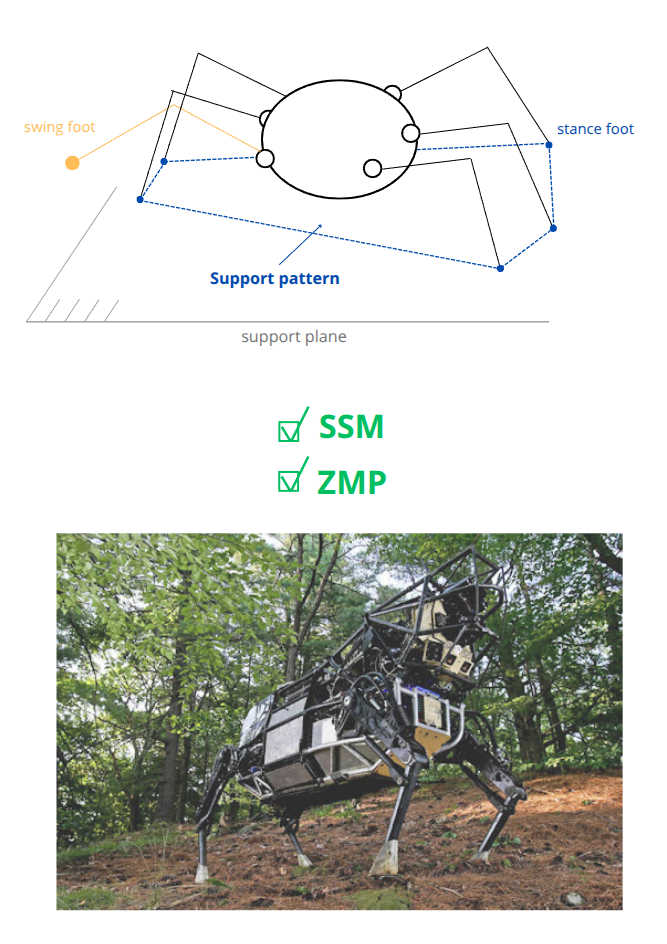
\includegraphics[scale=0.2]{Images/img_ch3/roughterrain1.png}
    }
    \subfloat{
        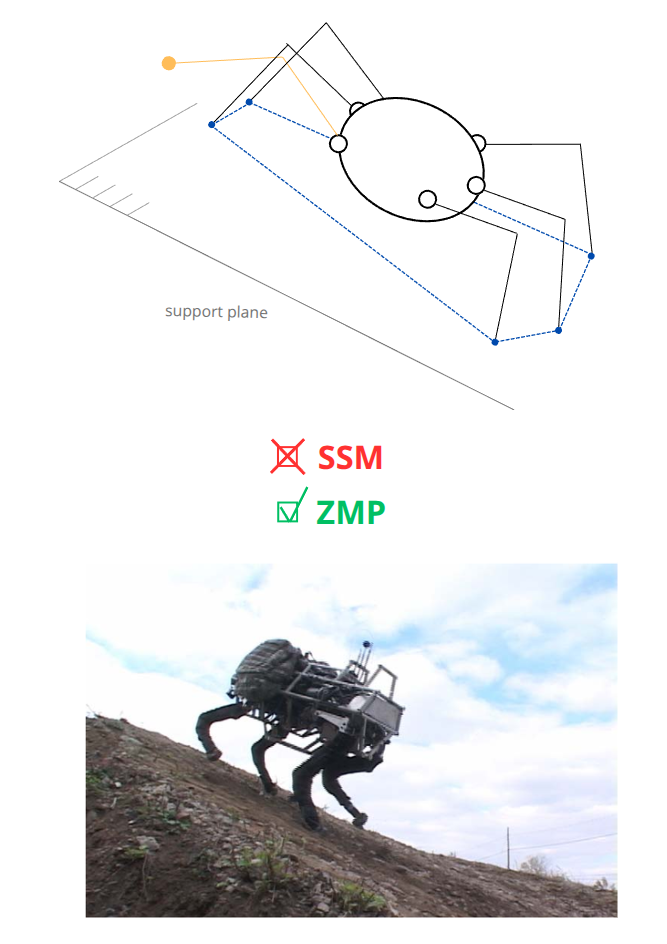
\includegraphics[scale=0.2]{Images/img_ch3/roughterrain2.png}
    }
    \subfloat{
        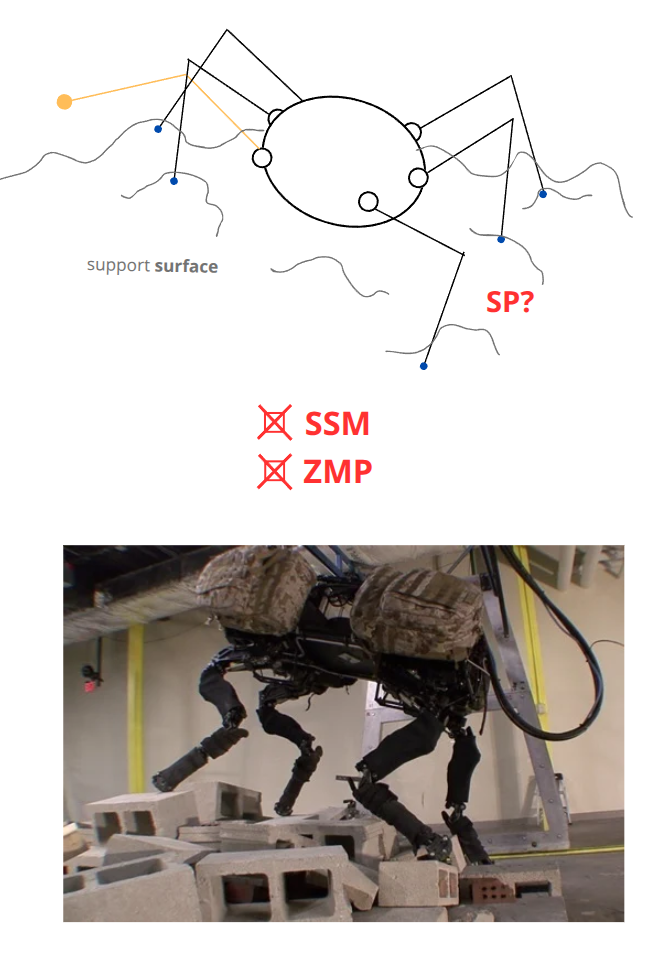
\includegraphics[scale=0.2]{Images/img_ch3/roughterrain3.png}
    }
    \caption[Overview of SSM and SMP usage]{Schematic representation of cases where SSM and ZMP can be used, with real-life examples based on Boston Dynamics Big Dog\cite{BigDogRoughTerrain}}
    \label{fig:rough_terrain}
\end{figure}


 S.Hirose, another pioneer of legged robotics, defined the tumble stability (TS) as a dynamic equilibrium criterion\cite{TumbleStability}. Identifying the tumbling axis as the line connecting two different contact points ($\overline{\mathbf{P}_{c,j}\mathbf{P}_{c,k}} \;, \; j,k \in J_c\ ;,\; j \not= k$), and the tumbling moment $\mathbf{M}_{j,k}$ as the total moment around the tumbling axis, computed from the effect of gravitational, inertial and external forces\cite{Ribeiro2023reaction}\cite{KentaroUnoPhD}.
 Under no slipping condition, the equilibrium is ensured when tipping over is counteracted by another contact foot. 
 Details on the computation of $\mathbf{M}_{j,k}$ and the stability constrain formulation are out of this scope, the resultant stability margin coming from this analysis is the tumble stability margin: 
\begin{equation}
\label{eq:TSM}
    TSM =\min_{j,k \in J_c}{\frac{\mathbf{M}_{j,k}}{mg}}
\end{equation}
where $m$ denotes the total mass of the robot. 

The tumble stability concept has been extended by W.Ribeiro for applications in microgravity, introducing the concepts of gravito inertia acceleration (GIA) and stability polyhedron\cite{GIA_polyedron}\cite{Ribeiro2023reaction}. 
The GIA is a vector derived from the combination of the robot's inertial acceleration and the gravity vector, while the support polyhedron is a 3D region defined from tumble stability constraints.
While the previously introduced support pattern is a 2D region, and the stability is evaluated with the ZMP or CoM projection, the GIA vector, introduces an additional dimension, and stability is guaranteed when the GIA vector is contained in the support polyhedron (as represented in Fig.\ref{fig:GIA}).

\begin{figure}[H]
    \centering
    \subfloat[Stable limit plane .\label{fig:stableregion}]{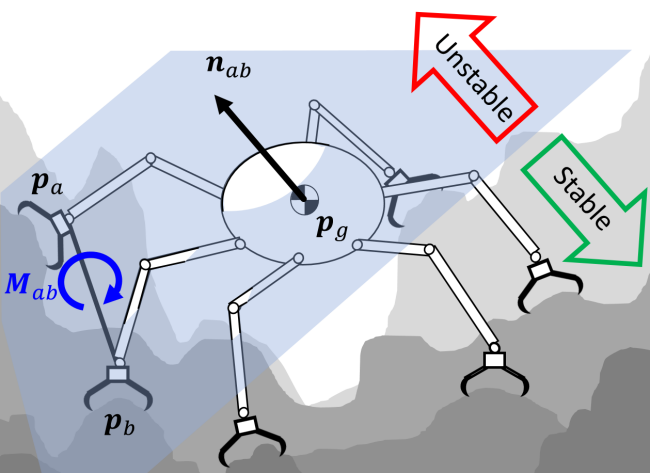
\includegraphics[scale=0.3]{Images/img_ch3/GIA1.png}}
    \subfloat[Stability polyhedron and GIA vector\label{fig:gia_polyhedron}]{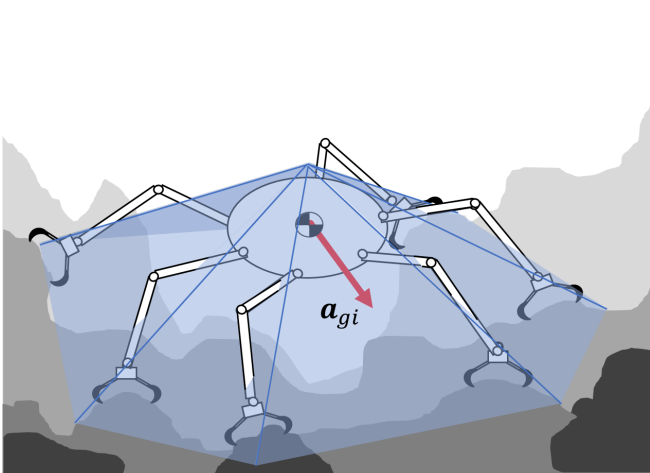
\includegraphics[scale=0.3]{Images/img_ch3/GIA2.png}}
    \caption[Schematic representation of GIA and support polyhedron]{\cite{GIA_polyedron}\cite{Ribeiro2023reaction} representation of GIA and support polyhedron configuration.}
    \label{fig:GIA}
\end{figure}



Both the TS and GIA can be formulated with gripping forces, making those methods suitable for climbing robots\cite{Ribeiro2019climbing}\cite{RibeiroGroundGripping}. 

The state of the art on stability analysis for legged robots is vast, in the next, additional criteria based on energetic considerations are described. 

\subsection{Energetic Stability}
\label{sec:gripping_stability}

For rough terrain, Messuri and Klein introduce an energy base criterion, the \textbf{energy stability margin} (ESM)\cite{ESM}, quantifying the minimum potential energy required to tumble the robot around the edge of the support polygon (a subset of the tumble axis, $\overline{\mathbf{P}_{c.k}\mathbf{P}_{c.k+1}}$ ):
\begin{equation}
\label{eq:ESM}
    ESM =\min_{k\in J_c}{mgh_k}
\end{equation}
In this formula, $h_k$ is the CoM height variation during the tumble, M is the total mass of the robot, and g is the gravitational acceleration. 

This index has been redefined  as \textbf{Normlaized Energy Stability Margin} (NESM) by Hirose, considering only the variation of the robot's CoM height \cite{NormalizedEnergySM}

\begin{equation}
\label{eq:NESM}
    NESM = \frac{ESM}{mg} = \min_{k \in J_c}{h_k}
\end{equation}

Both the ESM and NESM are efficient measures to evaluate statically stable walking on rough and sloped terrains\cite{EnergyIndexhexapod}, but when relevant dynamic effects influence motion (as fast locomotion or manipulation), these indices are not reliable. 
position
From the idea of Ghasempoor and Sepehri\cite{DESMidea} to measure wheel-based mobile manipulator stability, Garcia \cite{GarciaDESM} extend it for walking machines. 
The ESM has been extended, including the presence of other dynamical effects, like inertial forces or manipulation effects, computing the increase of mechanical energy that the CoM experiences during the tumble. 
The resulting \textbf{Normalized Dynamics Energy Stability Margin} (NDESM) is defined as the smallest of the stability levels required to tumble the robot around the support
polygon, normalized to the robot mass: 
\begin{equation}
\label{eq:NDESM}
    NDESM = \min_{k \in J_c}{\frac{E_k}{mg}}
\end{equation}
where $E_k$ identify the stability level of the $k^{th}$ edge of the support polygon,
which physically means the increment of mechanical energy required to tumble
the robot around that edge. 

In his extensive studies on the SILO 4 robot\cite{QuadrupedLocomotion}, Garcia introduce new approaches to the stability analysis, introducing new stability margins related to actuator limitation, such as: 
\begin{itemize}
    \setlength\itemsep{-0.7em} 
    \item \textbf{ torque limit stability margin}: related to the motor torque usage respect the limits
     \item \textbf{ current stability margin} related to the electric current usage respect the limits
\end{itemize}
Furthermore, normalized quantities and a global static-stability vector have been defined to analyze realistic constrained static stability, but the description of it is not relevant here.

\section{Performance Indices}
\label{sec:dynamic_indices}

The measures and criteria discussed until now address the evaluation of stability from geometrical, dynamic, and energetic considerations, but insights into system consumption efficiency and locomotion performance are not investigated. 

\subsection{Energetic Efficiency}
\label{sec:energetic_efficecny}

A possible energetic performance measure was proposed for a monopod robot\cite{SpecificResistance2}, based on the specific resistance $\varepsilon$ by Gabrielli and Von Karamn\cite{SpecificResistance1}, which considers not only the output power but also the mass moved and the obtained velocity. 
If $P$ denotes the output power, $m$ the total mass of the system, and $v_{max}$ the maximum speed of transportation, this quantity is defined as 
\begin{equation}
\label{eq:NESM}
    \varepsilon = \frac{P}{mgv_{max}}  
\end{equation}

This quantity can be evaluated in function of the locomotion  velocity as: 
\begin{equation}
\label{eq:NESM_2}
    \varepsilon(v) = \frac{P(v)}{mgv}  
\end{equation}
This can be used to compare different robots regardless of size, speed, or configuration.
An alternative way to compute this measure, comes from the definition of Gabrielli and von Karman\cite{SpecificResistance1}: 
\begin{equation}
\label{eq:NESM_2}
    \varepsilon = \frac{E}{mgd}  
\end{equation}
where $E$ is the total energy consumption for a travel of
distance $d$, $m$ is the total mass of the vehicle, and $g$ is
the acceleration due to gravity\cite{HandbookLegged}.

With a similar approach, energy consumption has been analyzed for a realistic six-legged robot\cite{EnergyIndexhexapod}, using the average locomotion power $P_{av}$ and the average velocity $v_{av}$ with the same formula as in Eq.\ref{eq:NESM_2}, denoting it as \textbf{specific energy consumption}.  
This same index has also been referred to as \textbf{cost of Transportation}(CoT)\cite{CosOfTransport} because it is a metric of the energetic economy of locomotion. 

Other interesting power efficiency indices have been introduced by M.F.Silva\cite{LocomotionPerformance}, such as the mean absolute power, mean power dispersion, and mean power lost, based on different power analyses on limb motors during locomotion.

\subsection{Mobility Efficiency}
\label{sec:mobility_efficecny}

When planning motion tasks for a limbed robot, stability, and efficiency should be taken into account, but dexterity and maneuverability are also important. 
For example, under the assumption of quasi-static motion in a horizontal plane, the SP criterion is used to evaluate stability, and according to the SSM, the optimal configuration (where the SSM is maximized) corresponds always to the one where the CoM project in the center of the SP. This requirement can lead to limb configurations close to singularities and joint limits(as represented in Fig.\ref{fig:bad_config}), degrading the dexterity of the system for any future motion.

\begin{figure}[H]
    \centering
    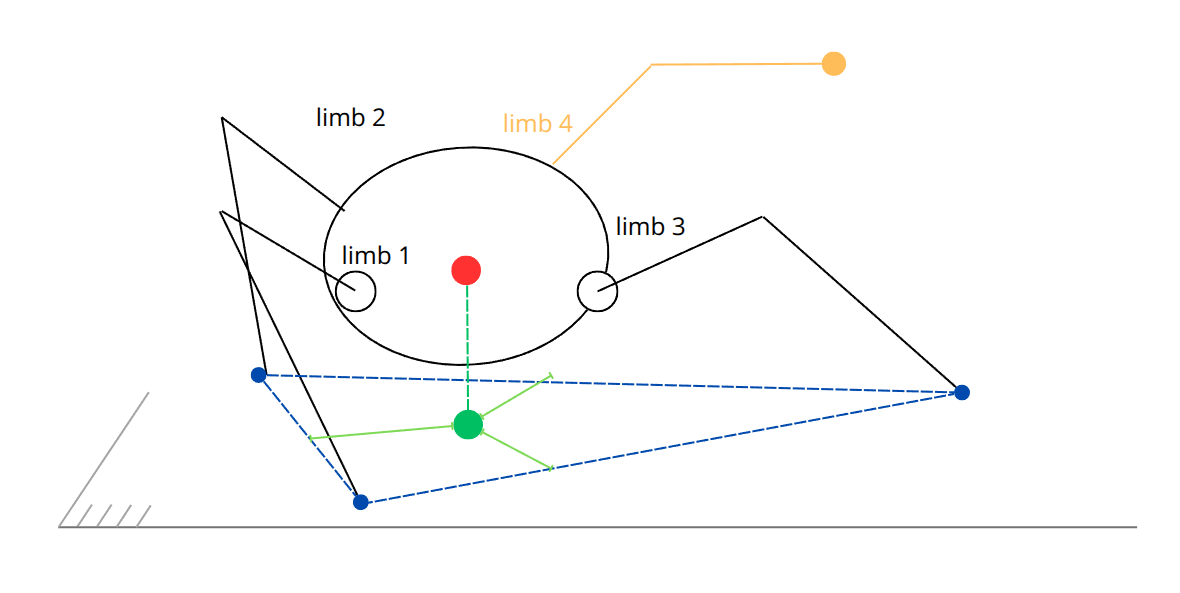
\includegraphics[width=0.7\textwidth]{Images/img_ch3/BadConfig.png}
    \caption{Example of undesired limbed robot configuration with optimal SSM}
    \label{fig:bad_config}
\end{figure}

The literature lacks a measure of ease of motion in a given configuration for multi-limbed robots, which could be relevant when planning complex multipurpose tasks.
In this section, the existing tools and research on limbed robot locomotion performances are summarized, in the next, a new measure to generalize and quantify manipulability for limbed robots is defined and discussed. 

F.Silva\cite{LocomotionPerformance} defined a \textbf{Locomobility Measure} from the concept of arm manipulability\cite{ManipulabilityYoshikawa}, applied to the limb during motion. 
With the same notation of chapter \ref{sec:differential}, the Jacobian matrix relating the limb root with the foot end is $\mathbf{J}_j(\mathbf{q}_j)$, with $\mathbf{J_P}_j(\mathbf{q}_j)$ denoting the translational part, then the translational velocity manipulability ellipsoid is described by the $3\times3$ positive definite matrix $\mathbf{J_P}_j(\mathbf{q}_j)\mathbf{J^T_P}_j(\mathbf{q}_j)$. 
Then, the locomobility index over a gait cycle $T$ is computed as: 
\begin{equation}
\label{eq:Locomobility}
    L_F = \frac{1}{T} \int_0^T{E_F(t)dt}  
\end{equation}
Where $E_F$ denotes the distance between the center of the foot translational ellipsoid and its intersection with the tangent to the desired foot trajectory. 
The best foot trajectory is the one that maximizes $L_F$. 
This index is useful to optimize the ease of foot motion along the trajectory during walking.

Another measure of the system locomotion capability is the workspace (def.\ref{def:workspace} in the previous chapter), which can be mapped from the limb tip to the reachable base positions, considering closed kinematic chain constraints in the contact points (with parallel manipulator model). This is a measure often used in the design phase for robot limbs, but rarely used in the base position space \cite{HexapodBaseWorkspace}\cite{HexapodBaseWorkspace2}. In free space, the limb workspace depends just on its mechanical design and joint limits, and after the limb development, it is fixed. The base workspace instead depends both on the contact limb workspace and contact points, which can be useful during foothold planning along the planned path \cite{LIMBEROTakadaThesis}\cite{LeggedPlanning1}\cite{threeLeggedDexterity}
. 

None of the measures described above provide an intuitive way to define optimal configuration in terms of base manipulability and dexterity. The only works with similar desired performance metrics are "general multi limb robots analysis" by C.Melchiorri \textit{et all} \cite{MultiLimbManipulabilityMelchiorri} and "velocity workspace analysis for multi-legged robots" by J.Lee \textit{et all}  
\cite{velocityWorkspacePolytope}.
In \cite{MultiLimbManipulabilityMelchiorri}, mobility, kinematic, and manipulability of multiple limb robots cooperating to move an object are analyzed. To define a generic framework for various similar systems (such as dexterous hands (multi-fingers interaction) and legged vehicles), the assumptions made on cooperation are very general.
This generality is both its strength and its limitation, it is complex to define, and not many examples of its usage can be found in literature.  

In \cite{velocityWorkspacePolytope} instead, walking robot velocity manipulability is analyzed with an approach similar to this research contribution, using the cooperative manipulators' parallelism introduced in section \ref{sec:leggedLimbedDK}. "Hard-foot" ground interaction is considered, constraining any moment to zero. With this model, the analysis has been conducted only for manipulability of translational base motion, represented through polytope\cite{PolytopesManipulability}. 


\section{Novel Base Manipulability Index}
\label{sec:base_manipolability}

As introduced in the previous section, the literature lacks tools to analyze online and intuitively the rotational and translational maneuverability of limbed robot configuration.
The only works trying to implement something similar are \cite{DualArmTaskManipulability} \cite{MultiLimbManipulabilityMelchiorri} for cooperative manipulators, and \cite{velocityWorkspacePolytope} for limbed robots. 
These works are 25 years old and applications based on these ideas cannot be found in literature.

Despite this, a measure of manipulability is very useful to define optimal task-consistent robot configuration, especially for multi-limb robots, where manipulation capabilities are intrinsic in limbs design.

To develop this theory, the manipulability ellipsoid (ME) is an intuitive and powerful geometrical entity to understand the capabilities of a robotic arm\cite{ManipulabilityYoshikawa}, and some researchers tried to adapt the theory for humanoid robots
\cite{BipedEllipsoid1}\cite{BipedEllipsoid2}\cite{BipedEllipsoid3}\cite{BipedEllipsoid4}\cite{BipedEllipsoid5}. This thesis contribution aims to break years of silence in research on manipulability theory for multi-limbed machines by showing the possibilities it can open up. Moreover, the need for this tool arose from the main problem addressed in this thesis, in fact it is used in chapter \ref{ch:chapter_five} to define properly an efficient adaptable motion sequence. 


Here, the \textbf{base ME} is introduced as an extension of the extensively used manipulators' ME theory, taking inspiration from the work of Professor B.Siciliano on space manipulability ellipsoids for multiple-arm systems\cite{MultiArmManipulability}\cite{DualArmManipulability}. Differently from \cite{MultiLimbManipulabilityMelchiorri} and \cite{velocityWorkspacePolytope}, his model is elegant, intuitive, and simple to use online, opening new possibilities for optimal motion adaptation at runtime, based on manipulability index maximization. 

% Both T.Yoshikawa's theory\cite{ManipulabilityYoshikawa}
% \cite{YoshikawaRedundancy}\cite{YoshikawaRoboticsBook}\cite{TRManipulability} of ME for single manipulators and B.siciliano's one \cite{DualArmManipulability}
% \cite{MultiArmManipulability} for cooperative manipulators are explained in Appendix \ref{ch:appendixB}


\subsection{Multi-limb Robot Base Manipulability Ellipsoid}
\label{sec:multi_limb_coopmanipulators}

In this section, the hypothesis and the intuitions behind this modeling approach are introduced, and then the kinetostatic and differential kinematic model considered is reported. Finally, the extension of multiarm ME to multi-limb robot base manipulability ellipsoid (BME) is defined.

\subsubsection{Assumptions and Duality}
\label{sec:multi_limb_coopmanipulators}

The multi-limbed robot-multiarm duality is inspired by the similar behavior between the two systems (as schematically represented in Fig.\ref{fig:MultiArmLimbed}), and it is possible when the assumptions listed below hold.

As multiple arms with fixed bases cooperate to move an object in space, a multi-limb robot with fixed contacts reconfigures the limbs to move the torso. 
This behavior is based on the hypothesis of \textbf{contact limb motion propagation without penetration} (\textit{Assumption 1}), as introduced in section \ref{sec:leggedLimbedIK}, and represented intuitively in Fig.\ref{fig:BaseMotionIK}. 
From this, the similarity between the base of each manipulator and the corresponding limb contact point is clear.

Furthermore, tight grasp and rigid object\cite{MultiArmManipulability} is considered for the multiarm system (\textit{Assumption 2}), likewise, the limb root is mechanically attached to the robot torso. 

A schematic view of this is represented in Fig.\ref{fig:MultilimbMultiArm} below. 

\begin{figure}[H]
    \centering
    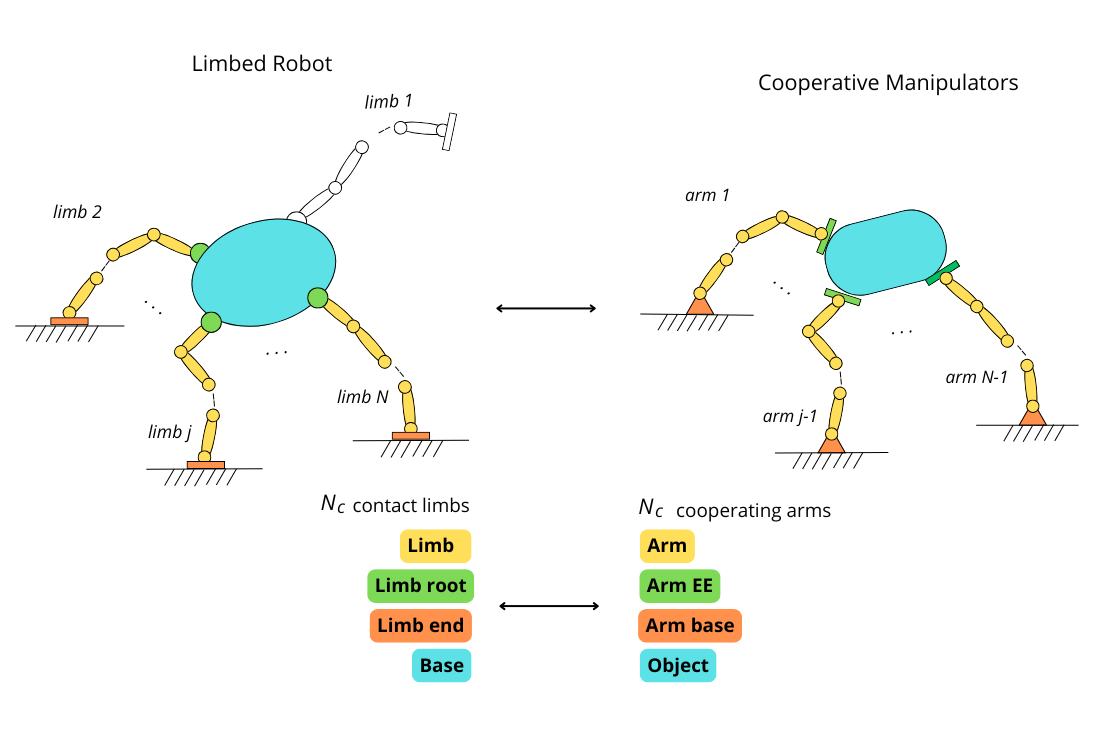
\includegraphics[width=0.9\textwidth]{Images/img_ch3/MultilimbMultiArm.png}
    \caption{Schematic representation of multi-limbed robots and cooperative arms duality}
    \label{fig:MultilimbMultiArm}
\end{figure}

\subsubsection{Kinematic Model for Multi-Limb Robot Base and BME}
\label{sec:multi_limb_coopmanipulators}

The derivation of the kinetostatic model for a multiarm system\cite{MultiArmManipulability} and the quantities involved are defined in \cite{MultiArmManipulability}, here the relevant quantities and equations are summarized for a multi-limb robot. All the vectors are measured in the base frame and represented in Fig.\ref{fig:multilimbmodel}.

\begin{figure}[H]
    \centering
    \subfloat[Frame references and DOFs.\label{fig:multilimbdof}]{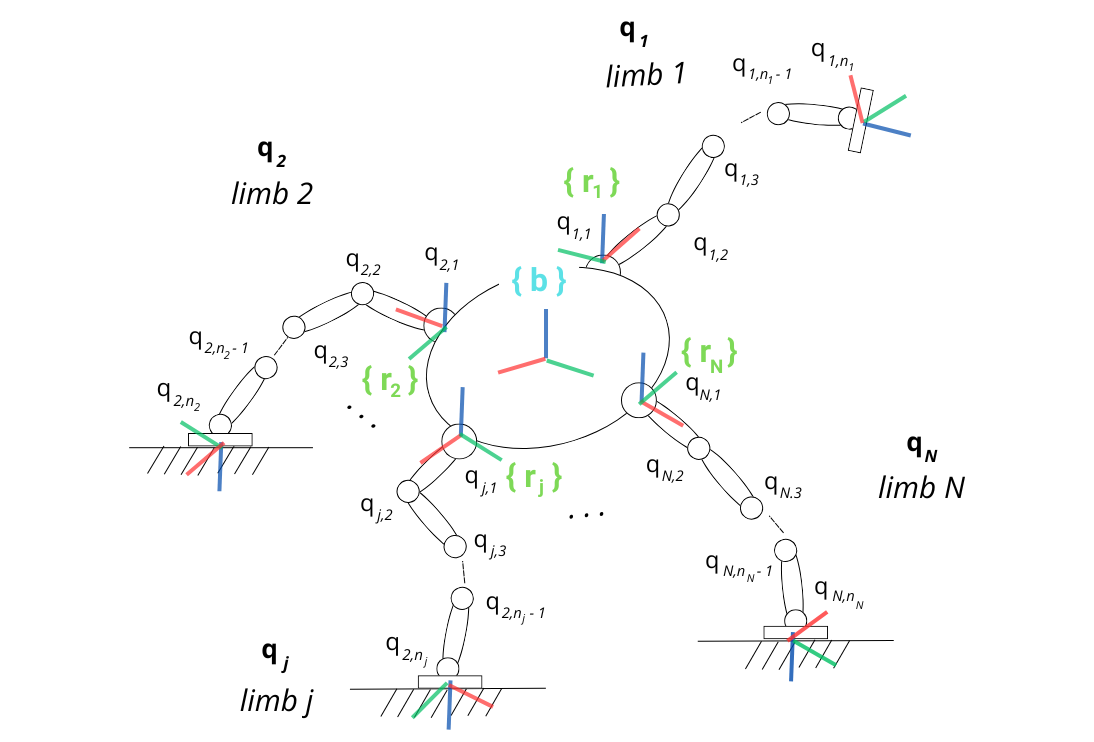
\includegraphics[width=0.8\textwidth]{Images/img_ch3/multilimbmodelDOF.png}}\\
    \subfloat[Relevant vectors.\label{fig:miultilimbvec}]{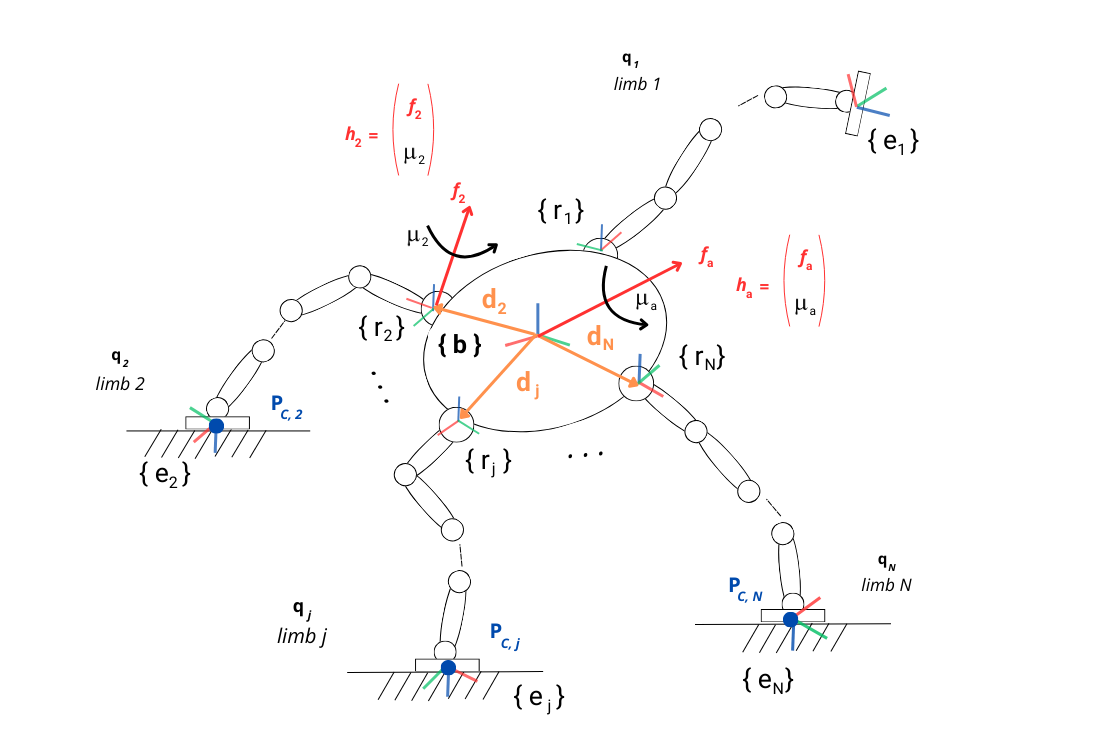
\includegraphics[width=0.8\textwidth]{Images/img_ch3/multilimbmodelVector.png}} 
    \caption[Multi-limb robots frames and vectors]{Relevant frames, DOFs and vector in multi-limb robots}
    \label{fig:multilimbmodel}
\end{figure}

\begin{figure}[H]
    \centering
    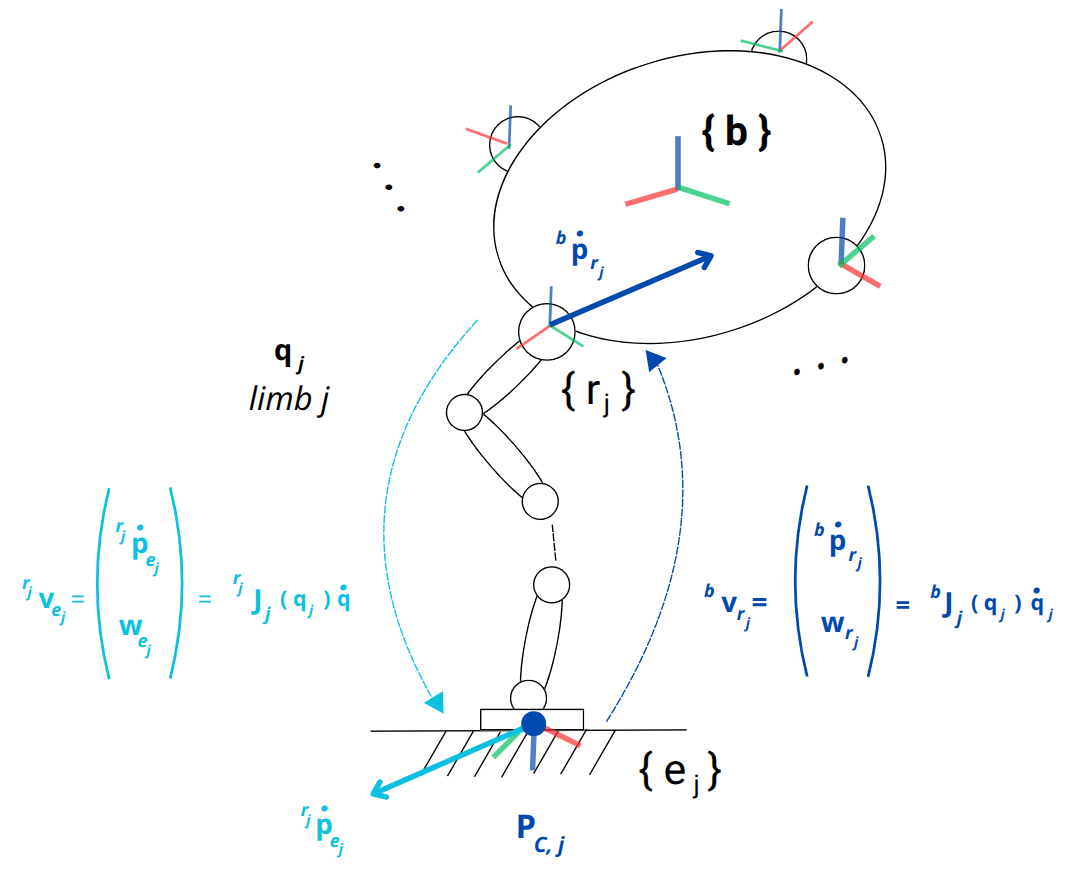
\includegraphics[width=0.6\textwidth]{Images/img_ch3/diffkin_multilimb.png}
    \caption{Schematic representation of single limb differential kinematic relation}
    \label{fig:diffkin_multilimb}
\end{figure}

$\mathbf{h}_a \in \mathbb{R}^{m}$
$\mathbf{h} \in \mathbb{R}^M , M = m\cdot N_c$

The vectors of generalized forces at the limb root, generated from ground contact interaction, are denoted as $\mathbf{h_i} \in \mathbb{R}^m$, and collected as $\mathbf{h} \in \mathbb{R}^M$ ($M = m\cdot N_c$).If the vector of external forces applied at the CoM of the base is denoted as $\mathbf{h_a}$, then: 
\begin{equation}
    \mathbf{h}_a = \mathbf{W} \mathbf{h}
    \label{eq:grasping_relation}
\end{equation}
Where $\mathbf{W} \in \mathbb{R}^{m \times M}$  is the grasping matrix, used to map limbs root interaction to base task space. defined as: 
\begin{equation}
    \mathbf{W} = [ \mathbf{W}_1 \dots \mathbf{W}_j \dots\mathbf{W}_N],\quad
    \begin{cases}
    \mathbf{W}_j = \mathbf{0} \in \mathbb{R}^{m\times m}  \quad \text{if } j\not \in J_c\\
    \mathbf{W}_j = \begin{bmatrix}
        \mathbf{I_3} & \mathbf{0_3} \\
        \mathbf{R}_j & \mathbf{I_3}    \end{bmatrix} 
        , \quad \text{if } j \in J_c
    \end{cases}
    \label{eq:grasping_relation_rev}
\end{equation}

With $\mathbf{R}_j$ responsible of performing the vector product $\mathbf{d}_j \times \mathbf{f_j} = \mathbf{R}_j\mathbf{f}_j$, where $\mathbf{d}_j$ is the vector from base frame to limb $j$ root measured in the base frame, as represented in Fig.\ref{fig:multilimbmodel}.

From the inversion of this relation,
and neglecting the internal forces $\mathbf{h_r} \in \mathbb{R}^{M-m}$, which are representative of the null space of $\mathbf{W}$ 
%as explained in Appendix \ref{ch:appendixB}, 
, it is derived: 
\begin{equation}
    \mathbf{h} = \mathbf{W}^\dag \mathbf{h}_a
    \label{eq:grasping_relation_rev}
\end{equation}
Then, using the same notation introduced in chapter \ref{ch:chapter_two}, Jacobian matrices that relate each limb joint velocities to limb root, in the base frame, are defined as in (\ref{eq:rootDK_baseframe}) (accordingly to \textit{Assumption 1}), as represented for a single limb in Fig.\ref{fig:diffkin_multilimb}.
\begin{equation}
    \label{eq:root_jacobian}
     \mathbf{^b J_j(q_j)} = - \mathbf{J^b_{r_j}}\mathbf{{^{r_j}J_j}(q_j)}
\end{equation}
Where $\mathbf{{^{r_j}J_j}(q_j)}$ is the jacobian matrix of limb $j$, computed considering the limb-tip as EE and the root frame $\mathbf{r_j}$ as the "fixed" base.  
Those Jacobian matrices are collected in 
$\mathbf{J}(\mathbf{q}) \in \mathbb{R}^{M \times n}$ as 
\begin{equation}
\label{eq:JacobianFormulaMultiLimb}
    \mathbf{J}(\mathbf{q}) = diag(\mathbf{^b J_1}(\mathbf{q_1}) \dots \mathbf{^b J_j}(\mathbf{q}_j) \dots \mathbf{^b J_N}(\mathbf{q}_N)) ,\quad
    \mathbf{J_j}(\mathbf{q}_j) = \mathbf{0} \in \mathbb{R}^{m\times n_j}  \quad \text{if } j\not \in J_c
\end{equation}

While joint torque vectors in $\mathbf{\tau} \in \mathbb{R}^n$.
the kinetostatic relation (\ref{eq:Static}) holds, with $\mathbf{\gamma}_e = \mathbf{h}$, so substituting (\ref{eq:grasping_relation}): 

\begin{equation}
    \mathbf{\tau} = \mathbf{J}^T_a(\mathbf{q})\mathbf{h}_a
    \label{eq:MultiLimbKinetostatic}
\end{equation}
Where $\mathbf{J}^T_a(\mathbf{q}) = \mathbf{J}^T(\mathbf{q})\mathbf{W}^\dag \in \mathbb{R}^{n\times m}$

From kinetostatic duality, denoting with $\mathbf{v}_a \in \mathbb{R}^m$, the absolute velocity of the base, it holds the dual of (\ref{eq:MultiLimbKinetostatic}): 
\begin{equation}
    \mathbf{v}_a = \mathbf{J}_a(\mathbf{q})\mathbf{\dot{q}}
    \label{eq:MultiLimbvel}
\end{equation}

Finally, from relation (\ref{eq:MultiLimbvel}) and (\ref{eq:MultiLimbKinetostatic}) the \textit{\textbf{external base force manipulabnility ellipsoid}} for the base (EBFME), and the \textit{\textbf{absolute base velocity manipulability ellipsoid}} (ABVME) are defined as follows: 
\begin{equation}
    \mathbf{h}^T_a [\mathbf{J}_a(\mathbf{q})\mathbf{J}^T_a(\mathbf{q})]\mathbf{h}_a = 1
    \label{eq:BEFME}
\end{equation}
\begin{equation}
    \mathbf{v}^T_a [\mathbf{J}_a(\mathbf{q})\mathbf{J}^T_a(\mathbf{q})]^{-1}\mathbf{v}_a = 1
    \label{eq:ABVME}
\end{equation}

The matrix $\mathbf{E}_a \in \mathbb{R}^{m\times m}$ represents the core of the EBFME's quadratic form, while its inverse is the ABVME's. 
When the limbs have at least 6 DOFs, $m = 6$ (task space includes both rotation and translation), and a 6-dimensional curve clearly cannot be visualized, but a numeric index like the manipulability measure proposed by Yoshikawa \cite{ManipulabilityYoshikawa} can be defined:
\begin{equation}
\label{eq:ManipulabilityMeasureBase}
    w_a(\mathbf{q}) = \sqrt{det(\mathbf{E}_a(\mathbf{q}}))
\end{equation}

From now on, the joints' dependency is implicit.
By analyzing the equation of the ellipsoid matrix, and decomposing the absolute base Jacobian matrix, it is possible to decompose also $\mathbf{E}_a$ in a translational and rotational part. Denoting with $m_P \leq 3$ the dimension of the translational task space, and $m_O \leq 3$ for the rotational one ($m = m_O + m_P \leq 6$), the base Jacobian is decomposed in its translational  ($\mathbf{J_P}_a \in \mathbb{R}^{m_P \times n}$) and rotational part($\mathbf{J_O}_a \in \mathbb{R}^{m_O \times n}$): 
$\textbf{J}_a = \begin{bmatrix}
    \mathbf{J_P}_a\\ \mathbf{J_O}_a
\end{bmatrix}$ 
Then the expression of the ellipsoid matrix is: 
\begin{equation}
\label{eq:BME_decoupled}
    \mathbf{E}_a = \begin{bmatrix}
        \mathbf{E_T}_a & \mathbf{E_{TR}}_a \\
        \mathbf{E^T_{TR}}_a & \mathbf{E_{R}}_a 
    \end{bmatrix}
\end{equation}
Where $\mathbf{E_T}_a \in \mathbb{R}^{m_P \times m_P}$ is the core of the translational BME (TBME),  
$\mathbf{E_R}_a \in \mathbb{R}^{m_O \times m_O}$
is the core of the rotational BME (RBME),
and $\mathbf{E_{TR}}_a \in \mathbb{R}^{m_P \times m_O}$ is a coupling matrix.

If decoupling is possible, translational motion is analyzed with $\mathbf{E_T}_a$, while rotational with $\mathbf{E_R}_a$, furthermore, information could be derived from the coupling matrix. When the complete decoupling cannot be proven, an approximation can be used.

Yoshikawa studied the decoupling of translational and rotational manipulability \cite{TRManipulability}, sometimes implicit in the robotic structure, as in spherical wrist manipulators  (where the three wrist joints meet in a single point). When the mechanical structure doesn't imply it, a rule of thumb can be used to measure the quality of the approximation.
For example, the ratio of the matrix norms
\begin{equation*}
z_T = \frac{{||\mathbf{E_T}_a||}_2}{{||\mathbf{E_{TR}}_a||}_2} \quad
z_R = \frac{{||\mathbf{E_R}_a||}_2}{{||\mathbf{E_TR}_a||}_2} 
\end{equation*}
When the ratio of the motion under analysis is big enough, the coupling is negligible and the approximation is possible. 
Then, even when $m = 6$, the overall EM $\mathbf{E_a}$ is decomposed in its components, and independent analysis of translational or rotational motion is possible.
In this case, the ABVME can be decomposed in translational (ATBVME) and rotational (ARBVME):
\begin{equation}
    \mathbf{\dot{p}}^T_a [\mathbf{E_T}_a]^{-1}\mathbf{\dot{p}}_a = 1
    \label{eq:ATBVME}
\end{equation}
\begin{equation}
    \mathbf{\omega}^T_a [\mathbf{E_R}_a]^{-1}\mathbf{\omega}_a = 1
    \label{eq:ARBVME}
\end{equation}

Next, this theory is applied to multi-limbed robots, computing the ATBVME and analyzing its meaning.

\subsection{Multi-limb Robots ME Examples and Extensions}
\label{sec:ME_multi_limb_example}

An intuitive description of the manipulability ellipsoid is useful for understanding the examples and results discussed in the next.

T.Yoshikawa\cite{TRManipulability} proposes the manipulability ellipsoid as a measure of "ease of arbitrary changing the position and orientation of the end effector at the rip of the manipulator". Defined by the mapping of a unit sphere in the velocity (force) joint space to the corresponding velocity (force) task space, resulting in an ellipsoid. By looking at the major axis of the ellipsoid, it suggests the direction in which the mechanical system performs better. In fact, the distance between the ellipsoid center and its surface is a measure of how the joint space unit sphere is mapped in the task space, then, it is a measure of the "transformation ratio".
S.L.Chiu describes\cite{TaskCompatibilityPosture} this relation by interpreting the manipulator as a mechanical transformer with joint velocity (force) as input and Cartesian velocity (force) as output. 

Furthermore, from kinetostatic duality, it can be proven that the matrix describing the quadratic form of the velocity and manipulability ellipsoids are one the inverse of the other. That means that the maximum VME axis corresponds to the minimum FME axis. 
With the mechanical transformer interpretation, the conservation of energy justifies the F/VME duality, as amplification in velocity transmission corresponds to a reduction in force transmission, and vice versa\cite{TaskCompatibilityEllipsoid}.

With this simple interpretation (rather than the equations previously derived), it is clear that the closer the VME is to a sphere, the better the end-effector can move isotropically along all task space directions \cite{Siciliano}. When the VME gets elongated along some directions, those are the preferred directions of motion, 
and in the limit case when one axis becomes null, task space mobility is lost in that direction, and the system is in a singular configuration. 

If the extension of the manipulability theory is correct, similar considerations should hold for multi-limbed robot base motion. 
Even if the BME is the main objective, from the aspects described above, it can be deduced that the manipulability theory is useful also in analyzing the performance of limbs on their own. Concepts of task compatibility\cite{TaskCompatibilityPosture} and ellipsoid tracking \cite{EllipsoidTracking} can be employed when defining limb tasks such as manipulation, grasping configuration while climbing, or the best direction to approach the ground.
Furthermore, When using a complex EE such as GRIEEL, optimal postures in wheel mode can be defined based on the ellipsoid shape, according to driving requirements in interacting with the ground. 



As a final consideration, the V/FME is a powerful tool not only for its intuitive interpretation but also for the ease of computation, which comes from the singular value decomposition of the manipulator Jacobian matrix\cite{Siciliano}\cite{YoshikawaRoboticsBook}. 
However, it presents some limitations a lot discussed in literature\cite{PolytopesManipulability}\cite{LimitsEllipsoid}, one of those is the unrealistic hypothesis of the hypershpere joint velocity domain $||\dot{\mathbf{q}}|| = \dot{\mathbf{q}}^T\dot{\mathbf{q}}\leq 1$, a polytope ( $-\dot{q}_{i,max} \leq \dot{q}_i \leq \dot{q}_{i,max}, i=1,\dots,n$) is usually a better domain.

Despite this limitation, results obtained by applying the VME theory to some multi-limbed robots provide usefull information, both for mechanical design and the configuration definition during task execution, as discussed now. 

The following examples are implemented in MATLAB, with base manipulability theory and multi-limbed robots' kinematic computation. The used code is open-source, and it can be found in this \href{https://github.com/AlePuglisi/limbed-robot-control}{GitHub} repository.

\subsubsection{Example 1: Quadruped with 3-DOFs Limbs}
\label{sec:BME_quadruped}

This example considers a simple 4-limbed robot where each limb has 3 DOFs anthropomorphic arm configuration (as the one in Fig.\ref{fig:antropomorphicDH}), and an insect leg topology\cite{Todd}\cite{KentaroUnoPhD}. 
Even if the anthropomorphic configuration is considered (attached to the base), the leg links are denoted in order as coxa, femur, and tibia, with joints B2C, C2F, and F2T. 
From now on, this robot will be called LimbedEx1. 
The DH parameters of the limb are reported in Tab.\ref{table:limb_ex1_1_DH}, and the robot is represented in Fig.\ref{fig:ex1_robot}, with all legs in the zero configuration $\mathbf{q_0} = \begin{bmatrix}
    0 & 0 & 0
\end{bmatrix}^T$ and in the initial walking configuration $\mathbf{q_W} = \begin{bmatrix}
    0 & -\pi/6 & \frac{2}{3}\pi
\end{bmatrix}^T$.

\begin{figure}[H]
    \centering
    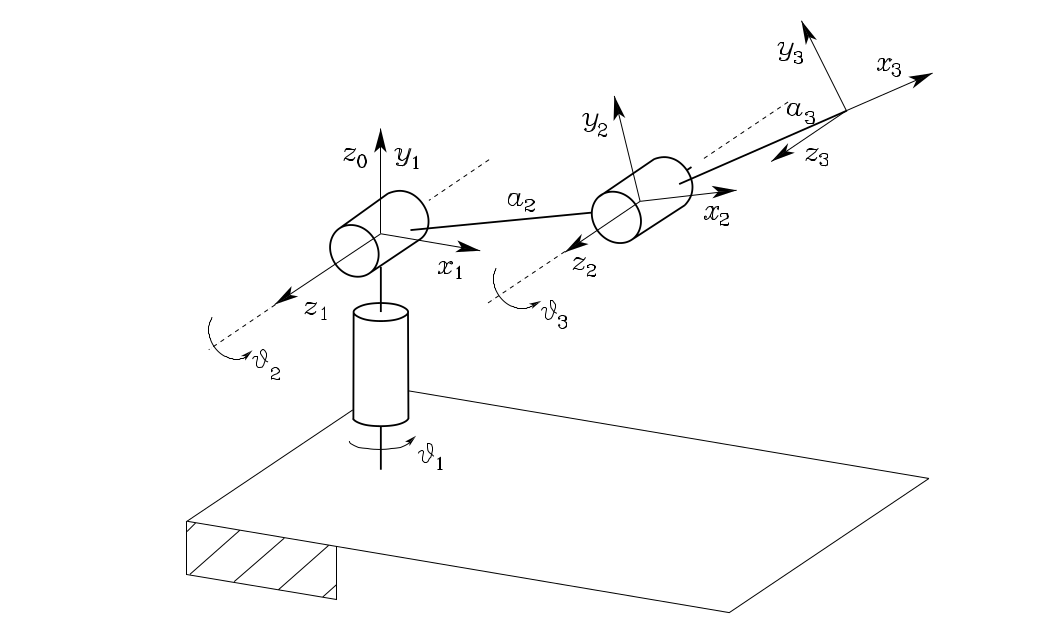
\includegraphics[width=0.6\textwidth]{Images/img_ch3/antropomorphicDH.png}
    \caption{\cite{Siciliano} representation of an anthropomorphic arm, with DH frames}
    \label{fig:antropomorphicDH}
\end{figure}

\begin{table}[H]
\centering 
    \caption{LimbedEx1 DH parameters}
    \label{table:limb_ex1_1_DH}
    \begin{tabular}{| l | c | c | c | c | c |}
    \hline
    \rowcolor{bluepoli!40}
%    \rowcolor{bluepoli!40}
     \textbf{Link} &  $a_i$ $[m]$ & $\alpha_i$ $[rad]$ & $d_i$ $[m] $ & $\theta_i$ $[rad]$ & $\theta_{offset, i}$ $[rad]$ \T\B \\
    \hline \hline
    \textbf{Coxa} ($i=1$) & 0.0 & $-\frac{\pi}{2}$ & 0.1  & $q_1$  & 0.0 \T\B\\
    \hline 
    \textbf{Femur} ($i=2$) & 0.35 & 0.0  & 0.0  & $q_2$  & 0.0  \T\B\\
    \hline
    \textbf{Tibia} ($i=3$) & 0.35  & 0.0  & 0.0  & $q_3$ & 0.0 \T\B\\
    \hline
    \end{tabular}
\end{table}

\begin{figure}[H]
    \centering
    \subfloat[LimbedEx1 with limbs in $\mathbf{q_0}$\label{fig:quadruped_q0}]{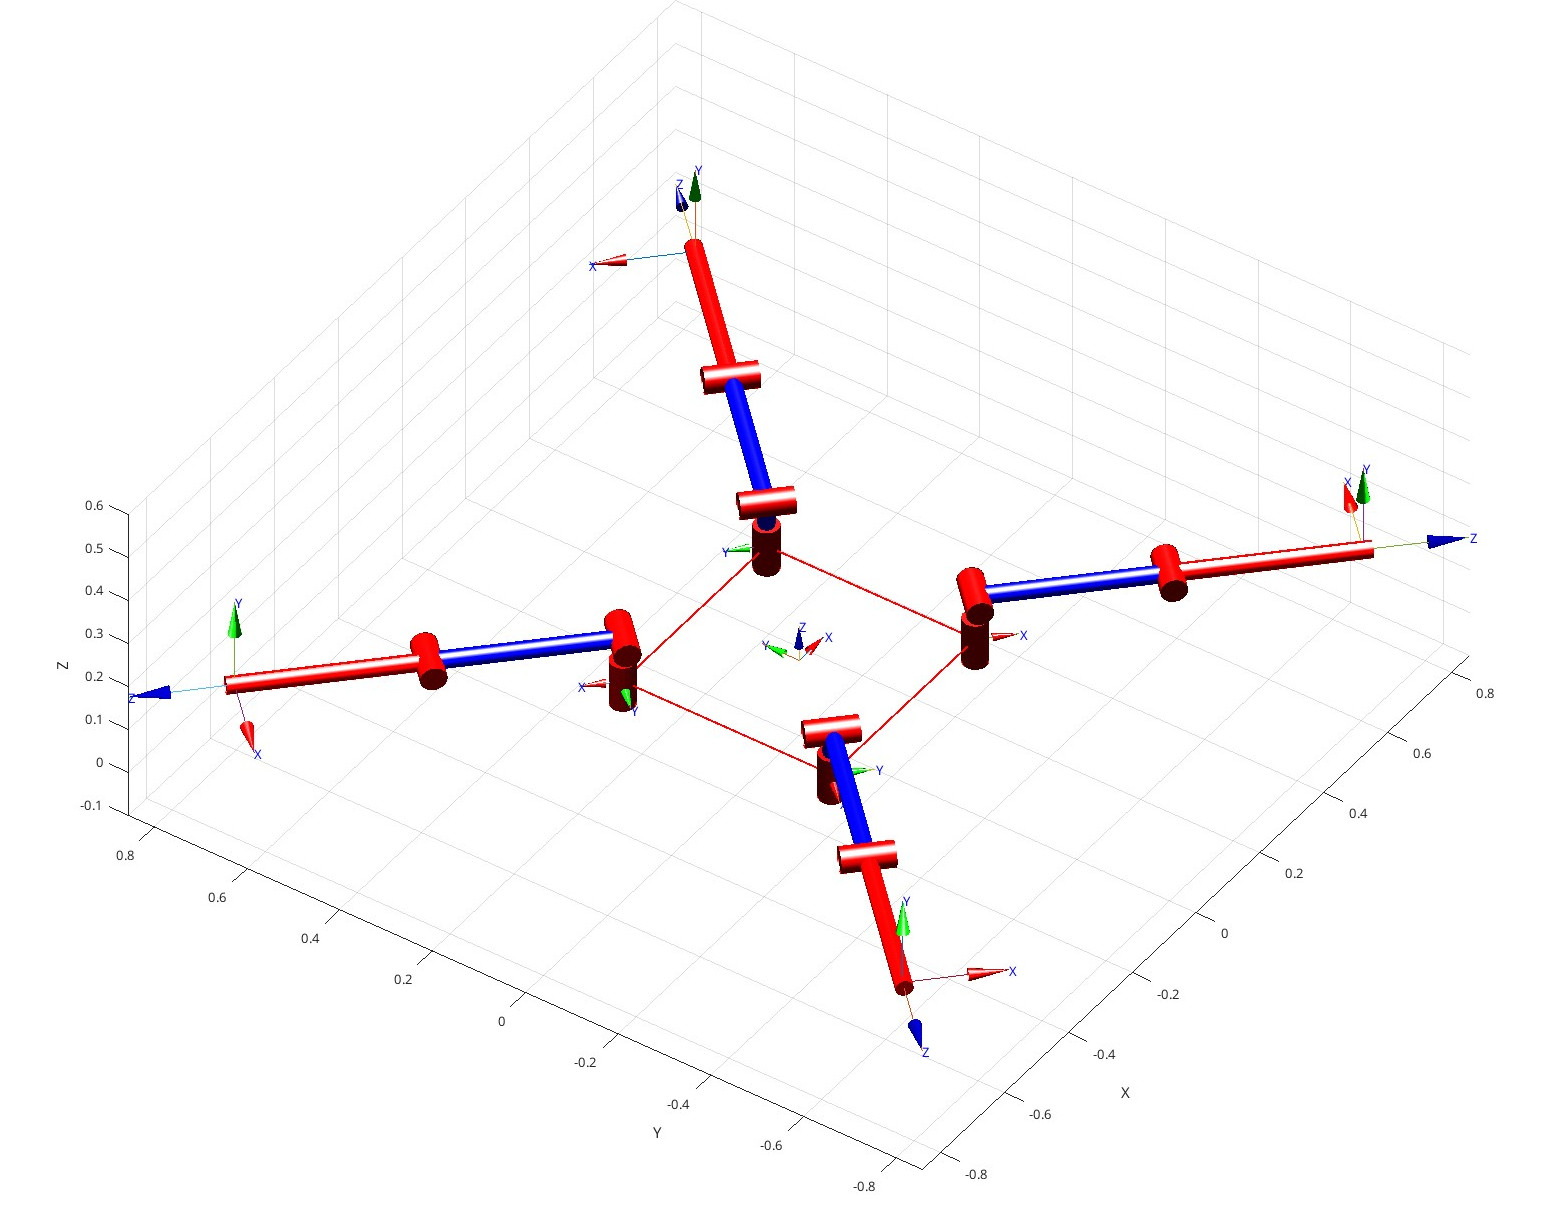
\includegraphics[width=0.45\textwidth]{Images/img_ch3/quadruped_q0.jpg}}
    \subfloat[LimbedEx1 with limbs in $\mathbf{q_W}$\label{fig:quadruped_qw}]{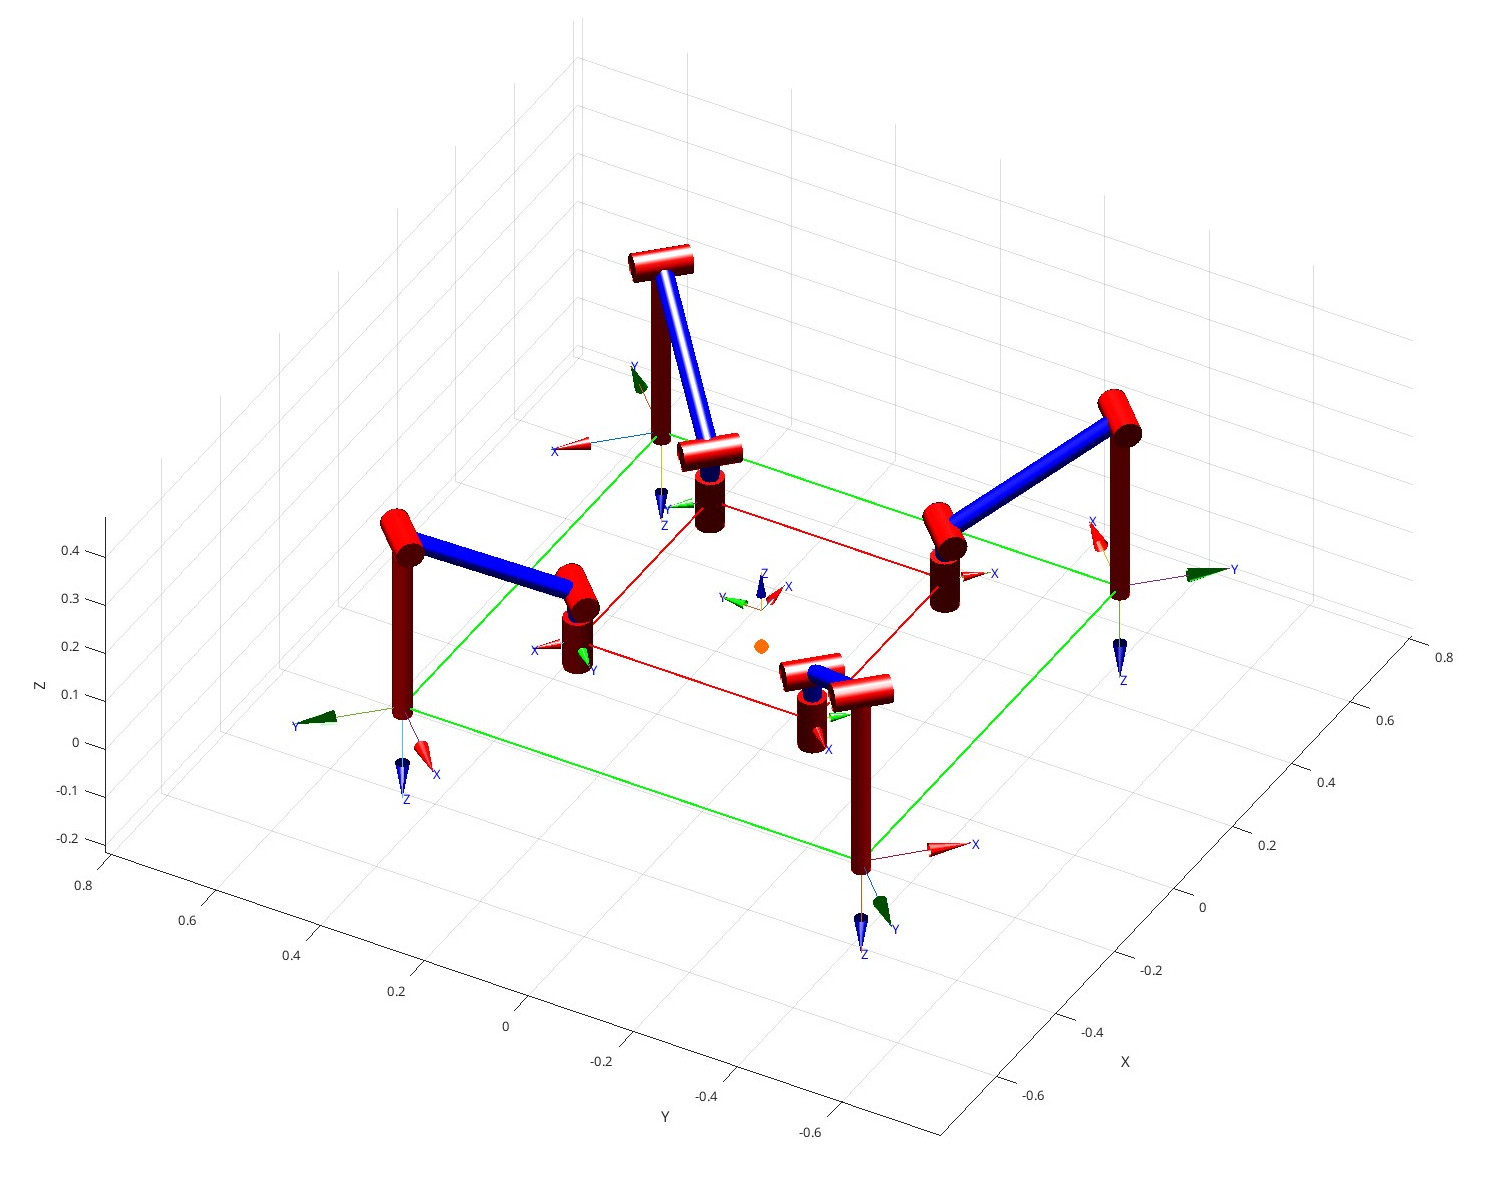
\includegraphics[width=0.45\textwidth]{Images/img_ch3/quadruped_qw.jpg}} 
    \caption[LimbedEx1 in zero and walking configuration]{LimbedEx1 in zero and walking configuration}
    \label{fig:ex1_robot}
\end{figure}

The results of the TVME of each limb and the ATBVME are now reported in different configurations.
Each limb TVME is represented to understand how they affect base motion, but also because the manipulability of the limb gives information on how it can interact with the environment when manipulating or approaching the ground, as described before. 

The figures will use the following convention: 
\begin{itemize}
    \setlength\itemsep{-0.7em} 
    \item\textbf{Robot torso}: Red polygon (connecting limb roots).
    \item\textbf{Base CoM}($\mathbf{P_CoM}$): Positioned in the base frame center.
    \item\textbf{Base CoM Projection}($\mathbf{\overline{P_CoM}}$): Orange point.
    \item\textbf{Support pattern}: Green polygon (connecting contact points). 
    \item\textbf{ATBVME}: Red ellipsoid (in the base frame). 
    \item\textbf{Contact limbs VME}: Blue ellipsoids (in the limbs EE frame). 
    \item\textbf{Contact limbs VME}: Green ellipsoids (in the limbs EE frame). 
\end{itemize}

The different configurations analyzed are computed as results of base motion translation tasks from the walking configuration, considering possible limb raises.

\textbf{Walking Configuration}
\begin{figure}[H]
    \centering
    \subfloat[perspective view\label{fig:ex1_walking_ortho}]{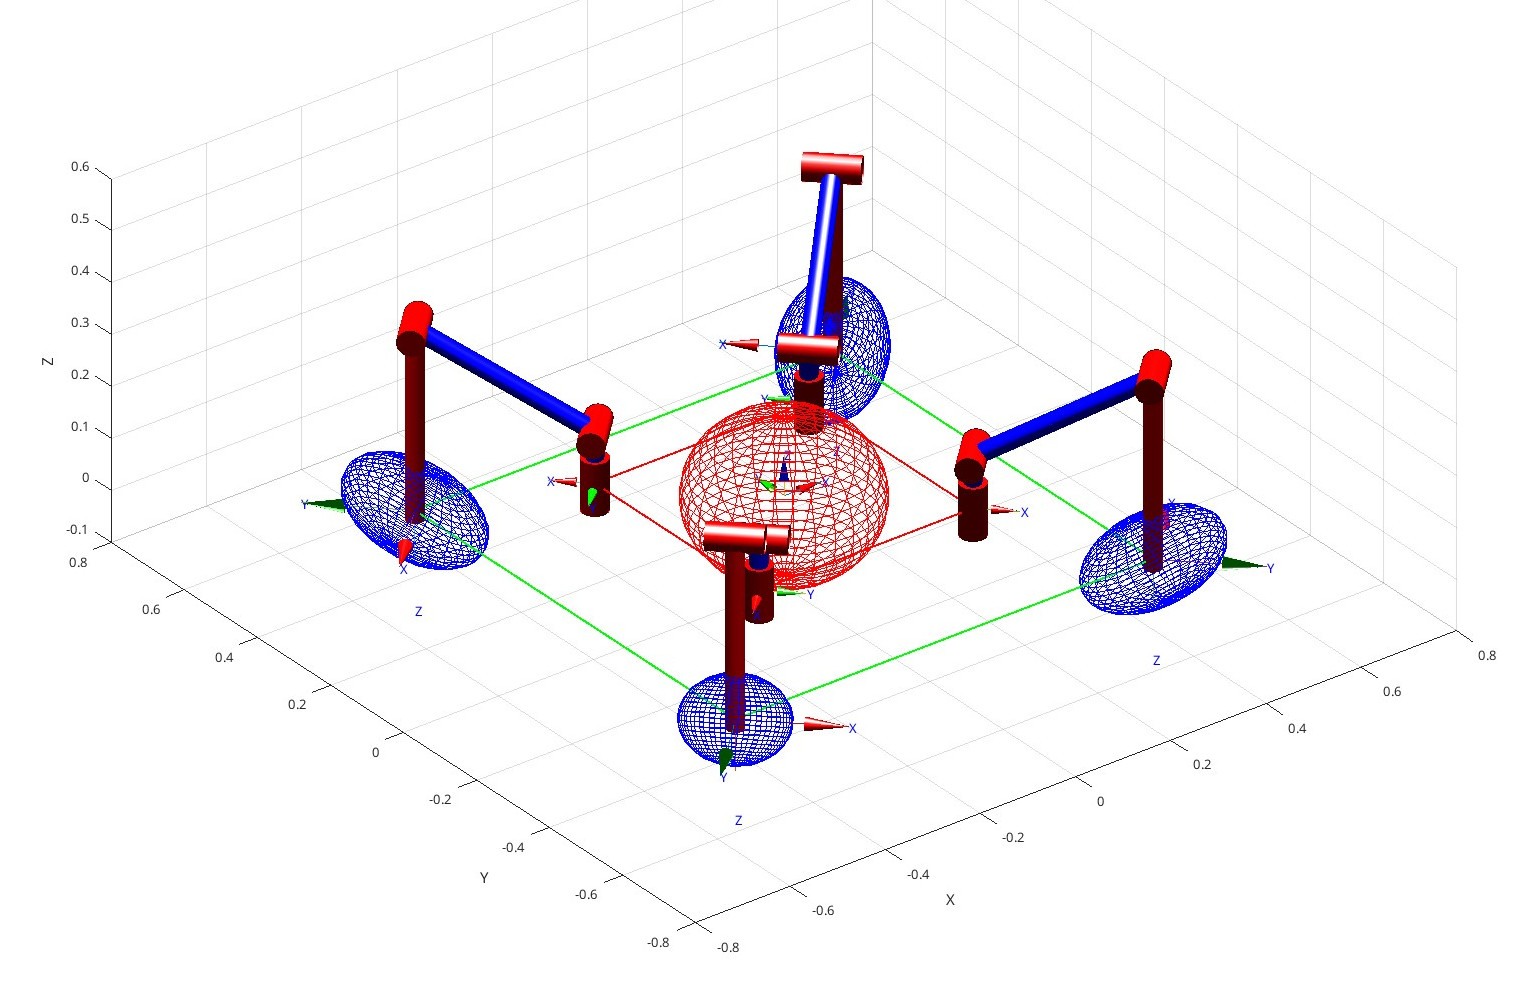
\includegraphics[width=0.3\textwidth]{Images/img_ch3/ex1_walking_ortho.jpg}}
    \subfloat[xy view\label{fig:ex1_walking_xy}]{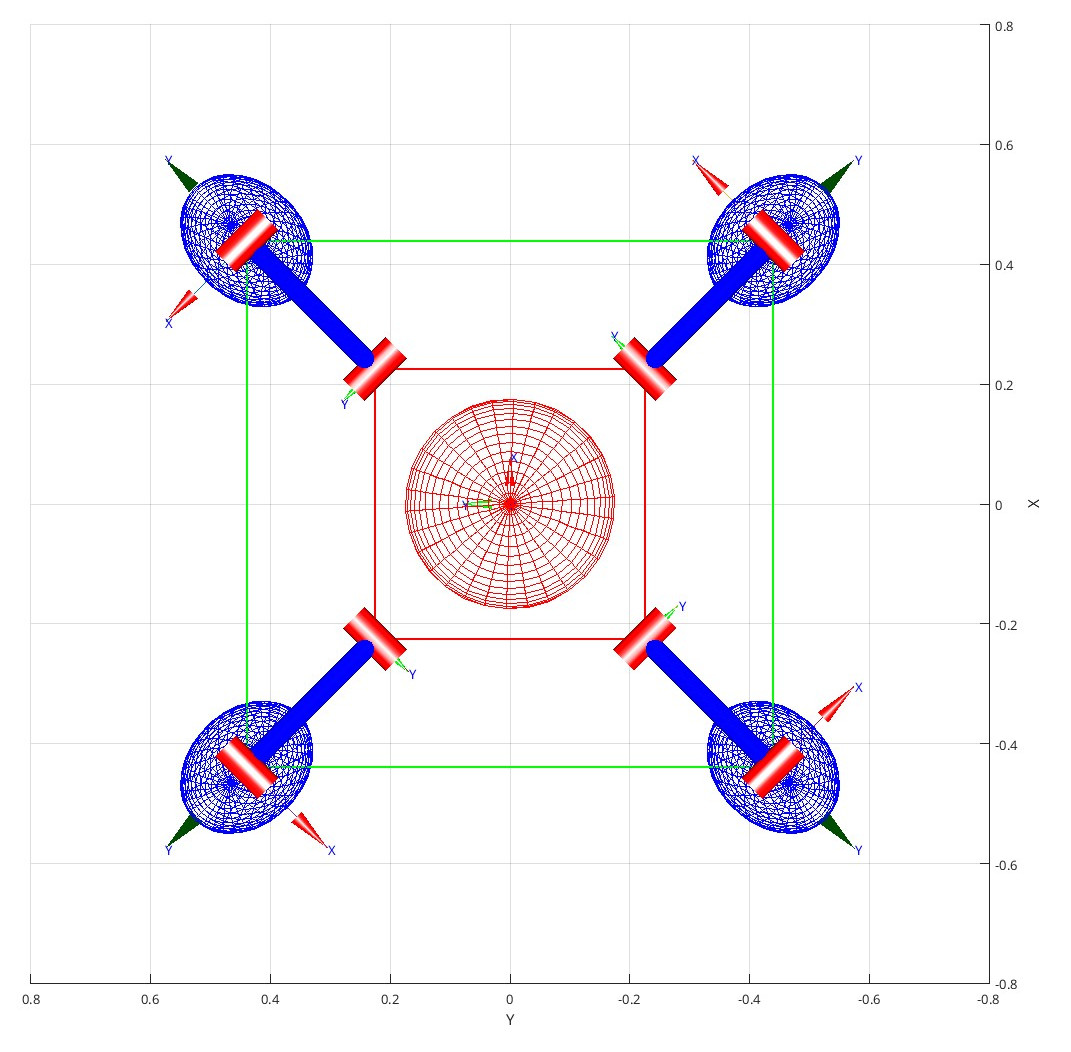
\includegraphics[width=0.3\textwidth]{Images/img_ch3/ex1_walking_xy.jpg}} 
    \subfloat[xz view\label{fig:ex1_walking_xz}]
    {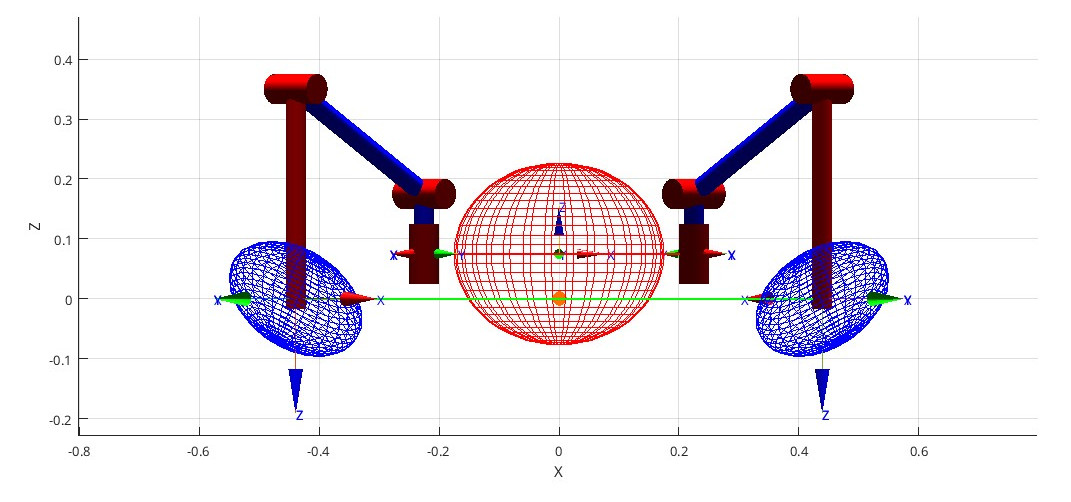
\includegraphics[width=0.3\textwidth]{Images/img_ch3/ex1_walking_xz.jpg}} 
    \caption[LimbedEx1 ME in walking configuration]{LimbedEx1 ME in walking configuration}
    \label{fig:ex1_walking}
\end{figure}

The characteristic isotropic shape of the ATBVME in Fig.\ref{fig:ex1_walking} is coherent with the expected mobility of the robot in this symmetric configuration, where motion in all directions is possible with the same dexterity.  

\textbf{Base z translations}

In this analysis, the manipulability measure is not explicitly reported. Still, recalling that it is proportional to the volume of the ellipsoid, it is simple to deduce how it is changing.

In those first tests, when the base translates along the positive z-axis, the shape of the ellipsoid gets flattened vertically, because of less mobility of the limbs in pushing the ground. This aspect of the ellipsoid axis relative dimensions is consistent, but the first problem of the BME theory is evident from the results in Fig.\ref{fig:ex1_z}. When the base is higher, the ellipsoid is stretched along the xy plane more than flattened in the z-axis, resulting in higher mobility. 
It is evident that "the higher the better" is not accurate when analyzing the dexterity of the base. 


\begin{figure}[H]
    \centering
    \subfloat[z=0.2, perspective view\label{fig:ex1_z020_xy}]{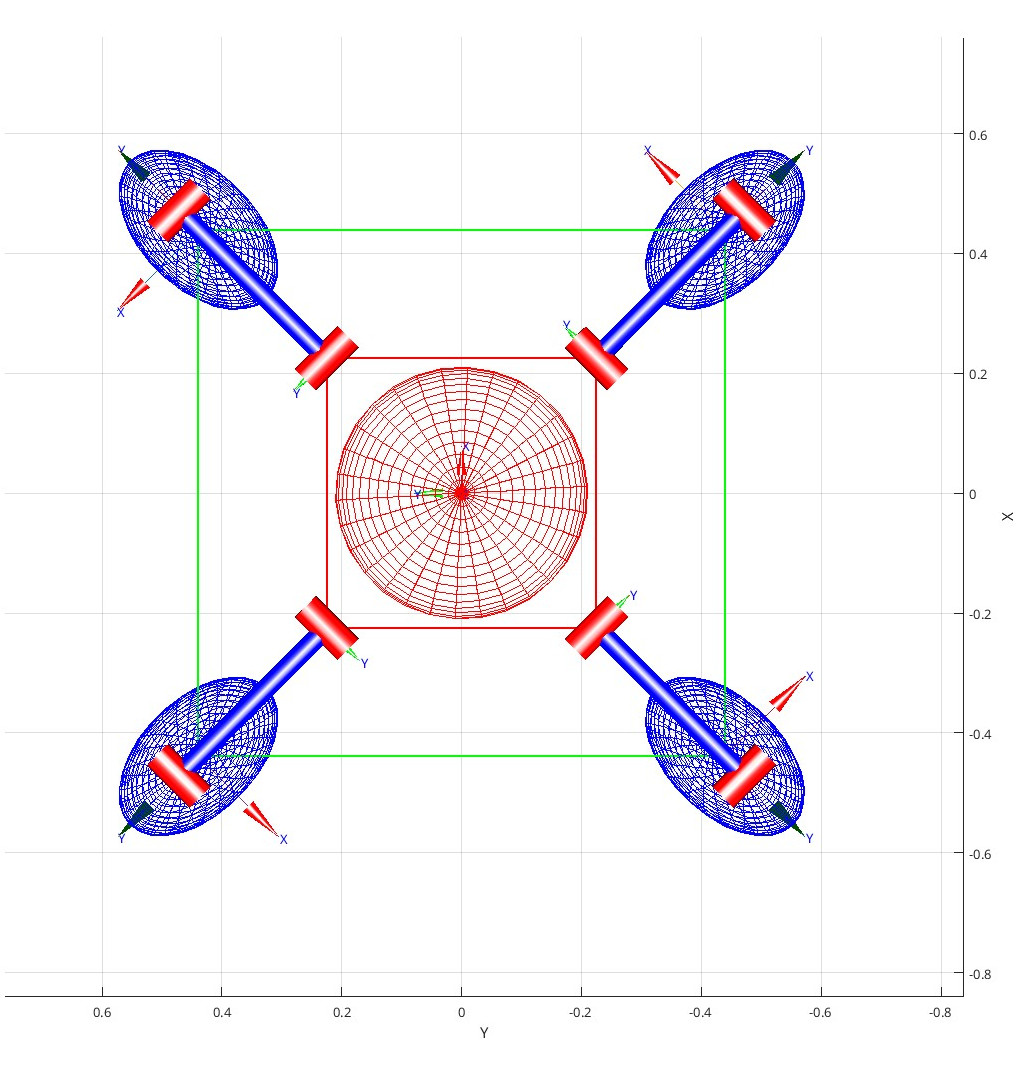
\includegraphics[width=0.35\textwidth]{Images/img_ch3/ex1_z020_xy.jpg}}
    \subfloat[z=0.2, xy view\label{fig:ex1_z020_xz}]{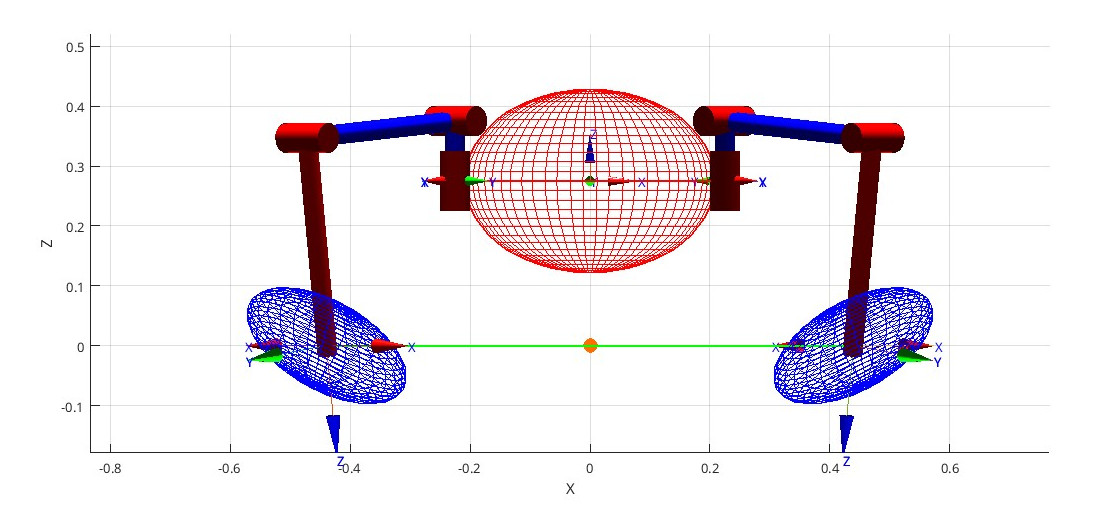
\includegraphics[width=0.35\textwidth]{Images/img_ch3/ex1_z020_xz.jpg}} \\
    \subfloat[z=0.4, xz view\label{fig:ex1_z040_xy}]
    {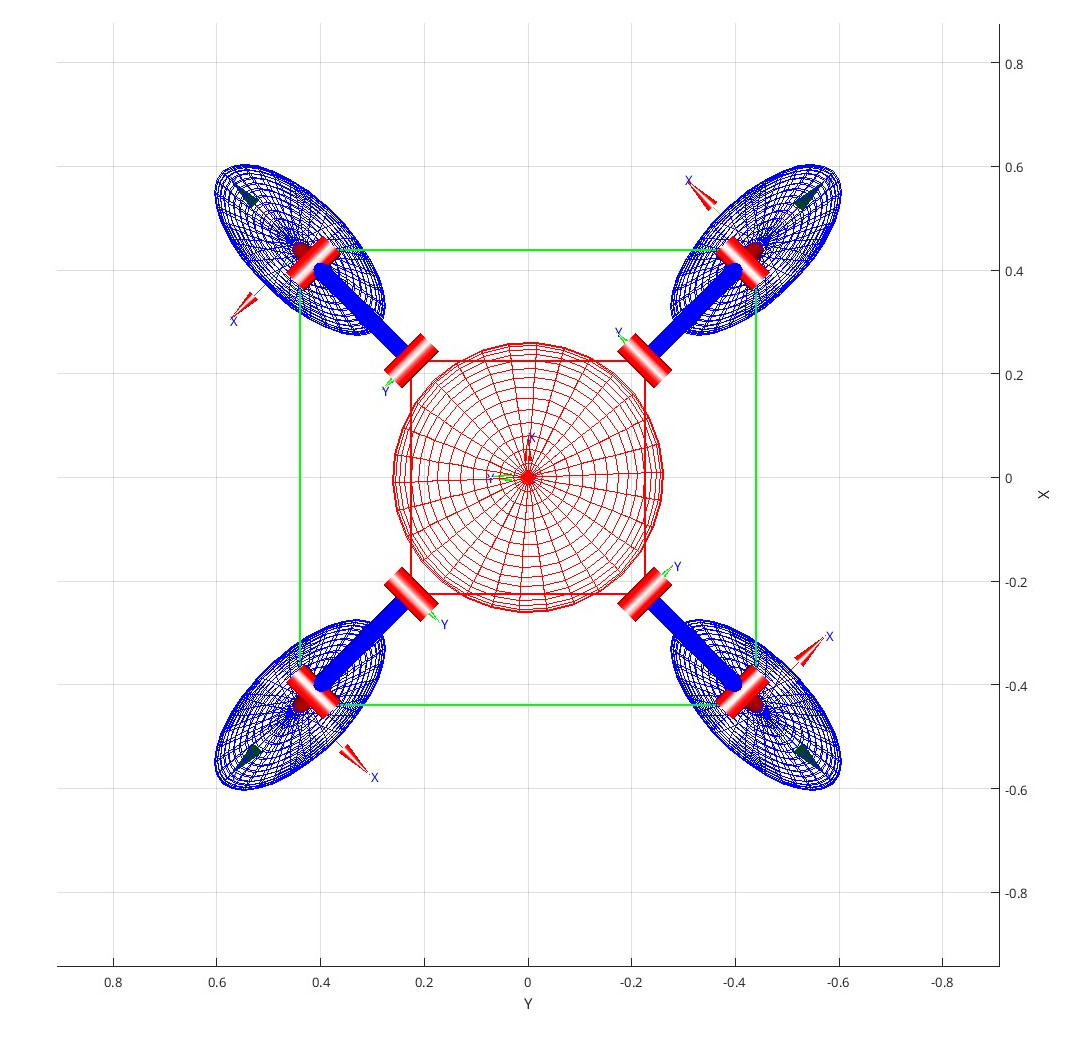
\includegraphics[width=0.35\textwidth]{Images/img_ch3/ex1_z040_xy.jpg}} 
    \subfloat[z=0.4, xz view\label{fig:ex1_z040_xz}]
    {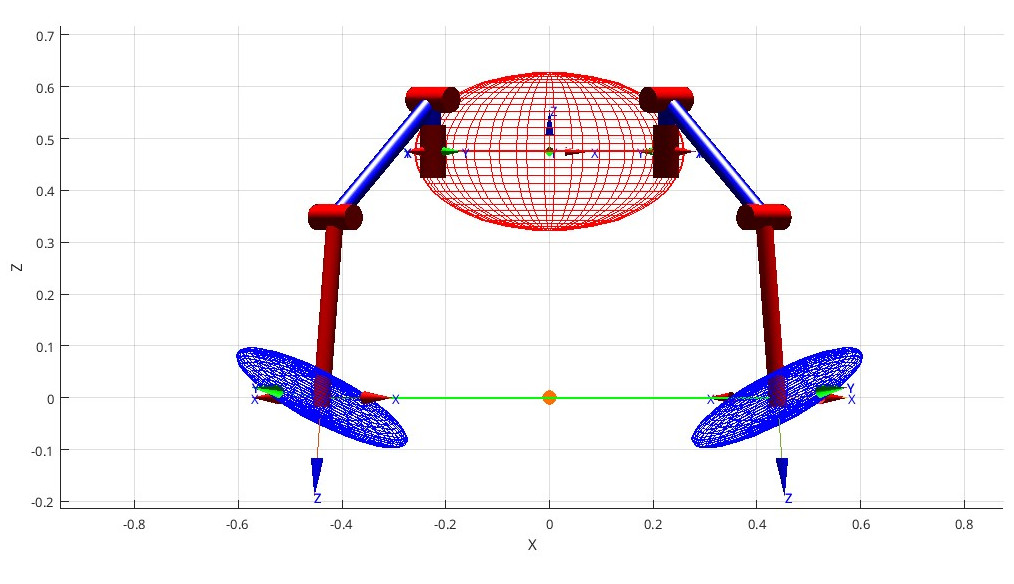
\includegraphics[width=0.35\textwidth]{Images/img_ch3/ex1_z040_xz.jpg}} 
    \caption[LimbedEx1 ME after z base translation]{LimbedEx1 ME after z base translation}
    \label{fig:ex1_z}
\end{figure}

\textbf{Base x,y,z translations}

Translating the base as in Fig.\ref{fig:ex1_xyz_translate} provides again coherent results in the sense of preferred motion directions, with the maximum axis of the ellipsoid orientated where the retracted limbs have a higher range of motion. But again the problem of the quantitative manipulability index is present, and even uncommon configurations such as the one in Fig.\ref{fig:ex1_z01_xneg01_yneg03_xy} result in satisfactory mobility. 

\begin{figure}[H]
    \centering
    \subfloat[z=0.1, x=0.15, xy view\label{fig:ex1_z01_x015_xy}]{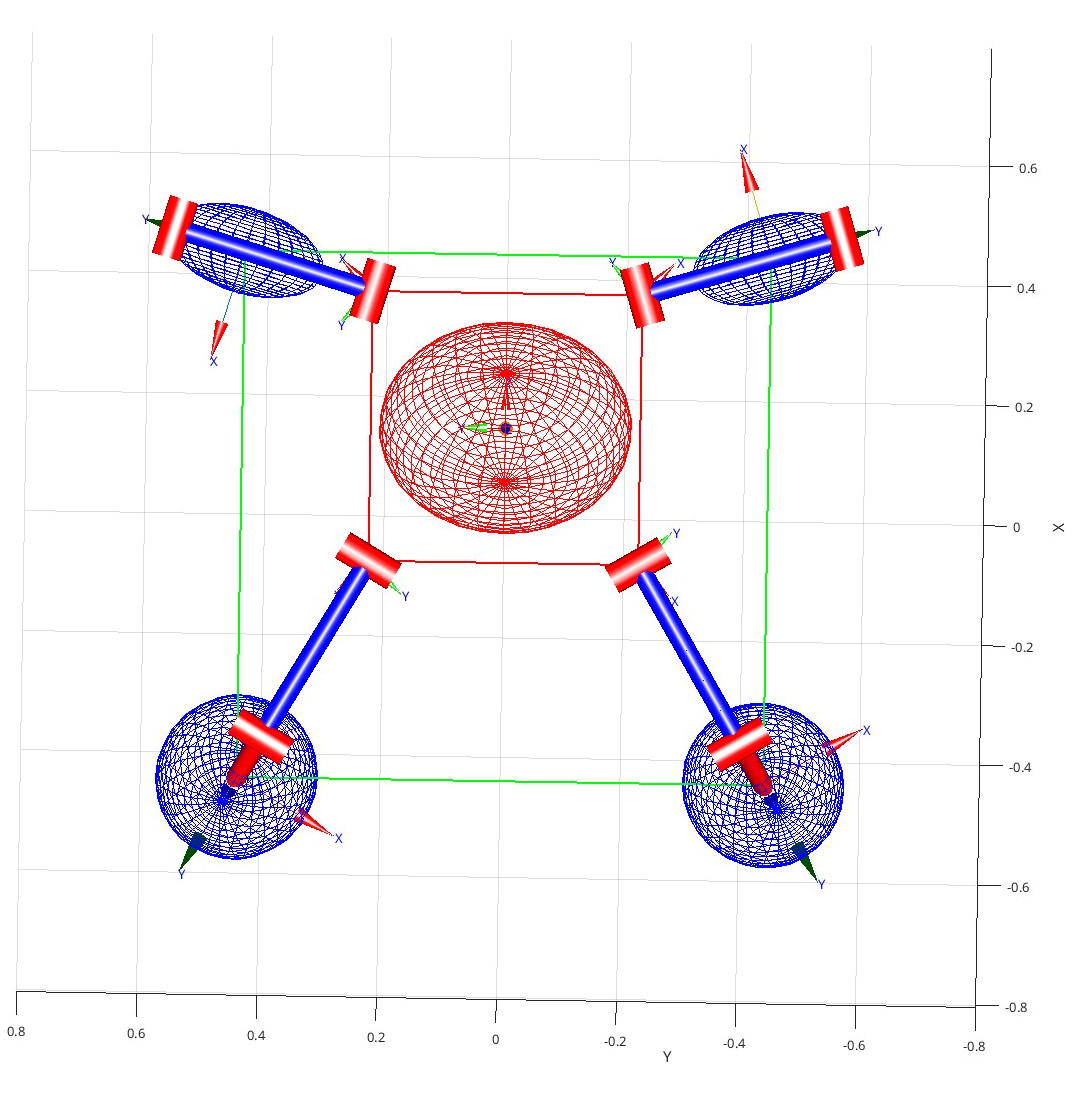
\includegraphics[width=0.35\textwidth]{Images/img_ch3/ex1_z01_x015_xy.jpg}}
    \subfloat[z=0.1, x=0.15, xz view\label{fig:ex1_z01_x015_xz}]{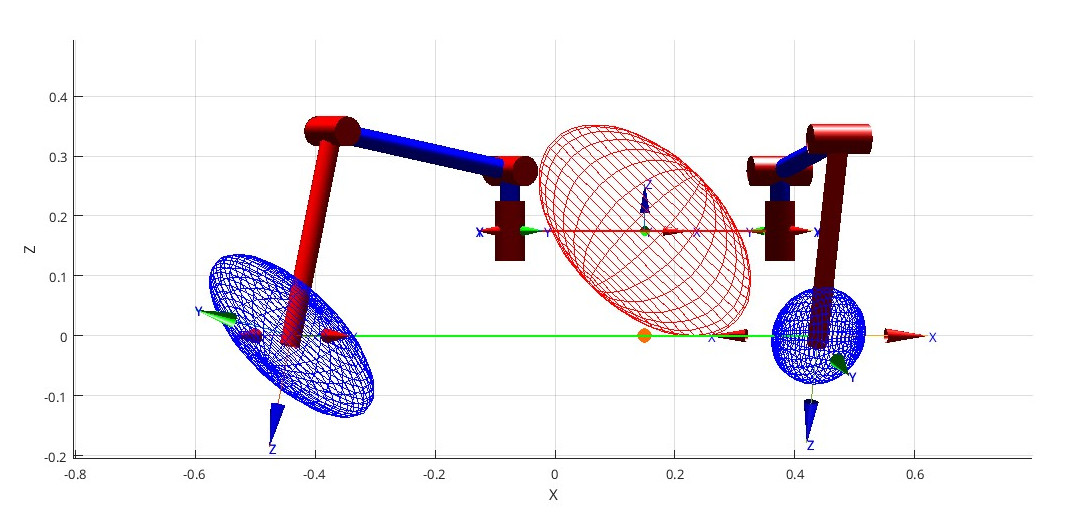
\includegraphics[width=0.35\textwidth]{Images/img_ch3/ex1_z01_x015_xz.jpg}} \\
    \subfloat[z=0.1, x=-0.1, y=-0.3, xy view\label{fig:ex1_z01_xneg01_yneg03_xy}]
    {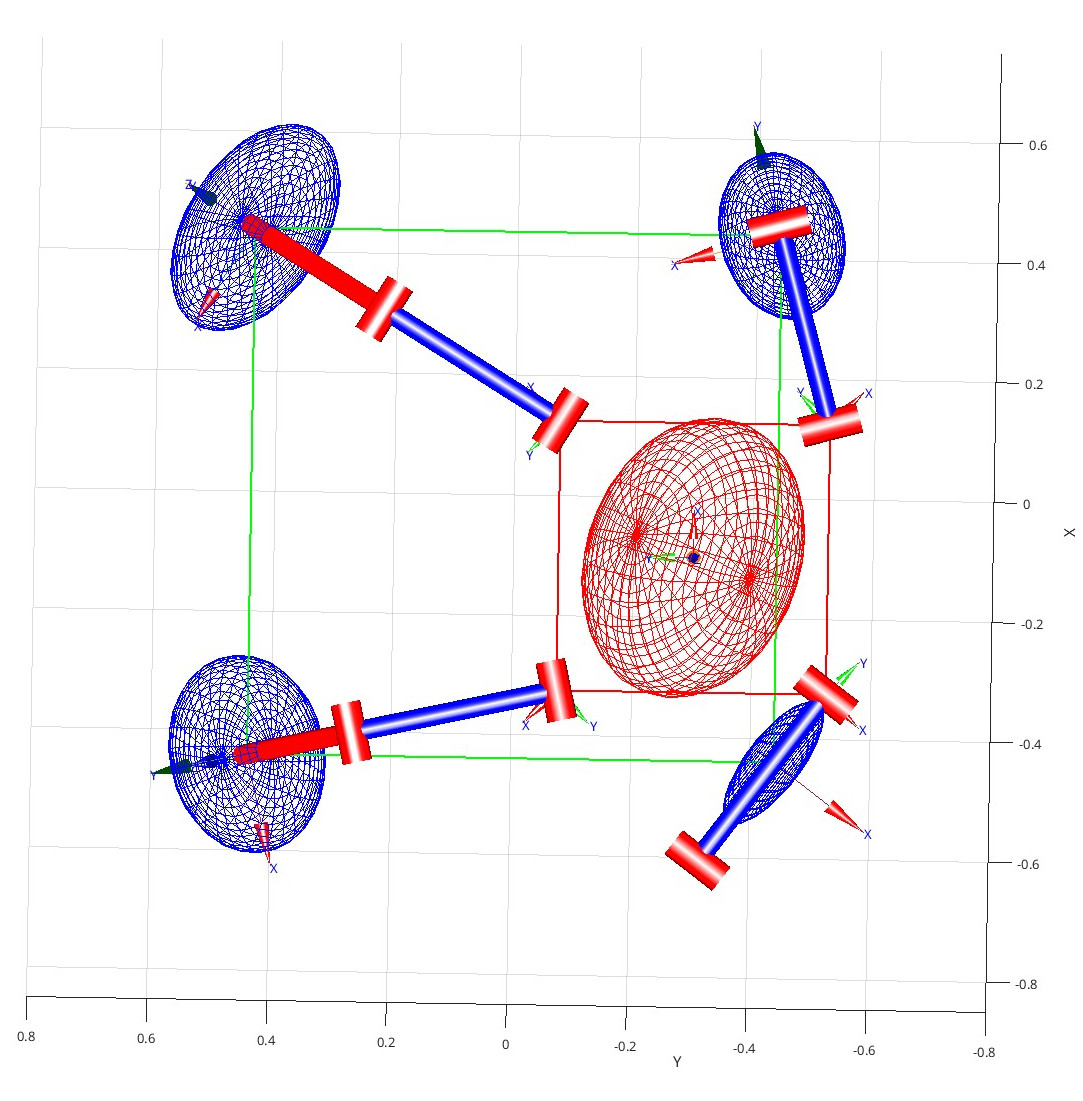
\includegraphics[width=0.35\textwidth]{Images/img_ch3/ex1_z01_xneg01_yneg03_xy.jpg}} 
    \subfloat[z=0.1, x=-0.1, y=-0.3, yz view\label{fig:ex1_z01_xneg01_yneg03_yz}]
    {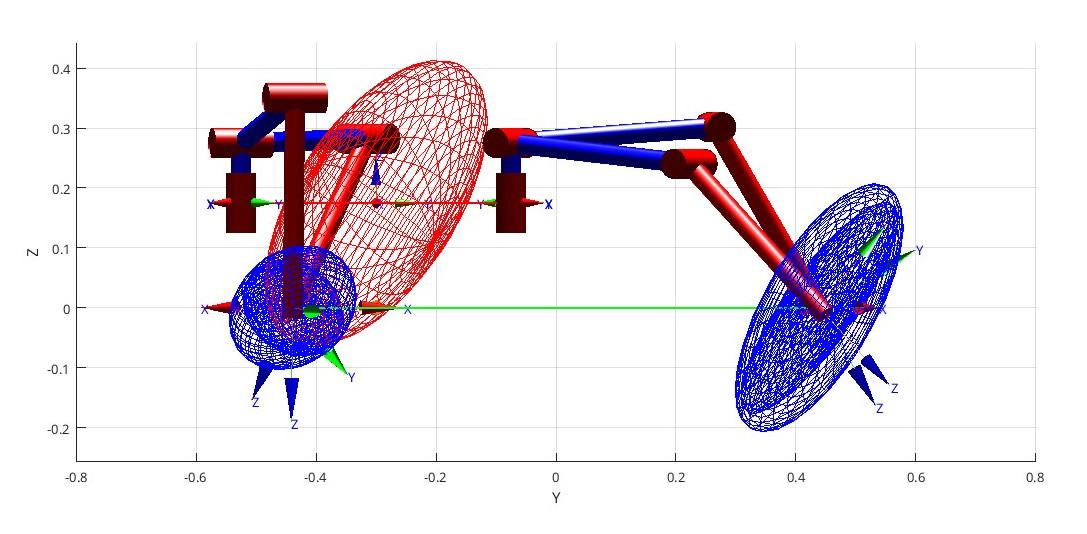
\includegraphics[width=0.35\textwidth]{Images/img_ch3/ex1_z01_xneg01_yneg03_yz.jpg}} 
    \caption[LimbedEx1 ME after generic base translation]{LimbedEx1 ME after generic base translation}
    \label{fig:ex1_xyz_translate}
\end{figure}

\textbf{Raise Limb}
When one limb is raised, only three limbs are used to move the base, and this is reflected in the distorted shape of the ellipsoid.
\begin{figure}[H]
    \centering
    \subfloat[z=0.1, and LF up, perspective view \label{fig:ex1_z01_LFup_ortho}]{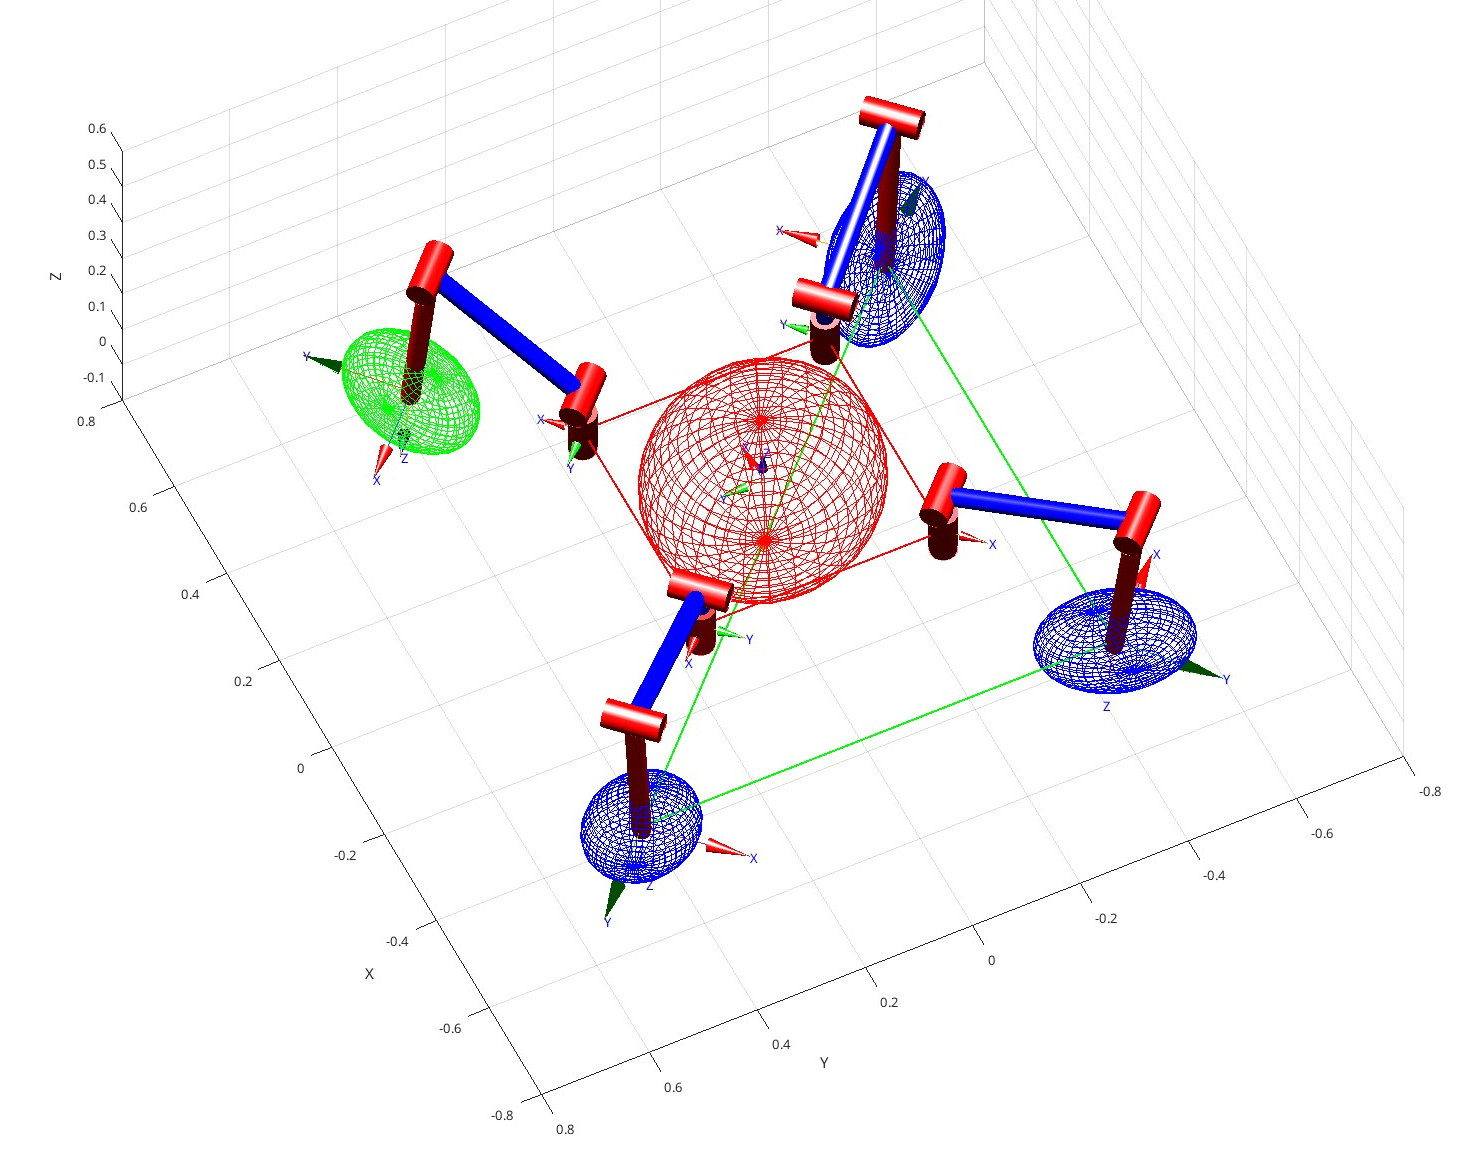
\includegraphics[width=0.35\textwidth]{Images/img_ch3/ex1_z01_LFup_ortho.jpg}}
    \subfloat[z=0.1, and LF up, xy view \label{fig:ex1_z01_LFup_xy}]{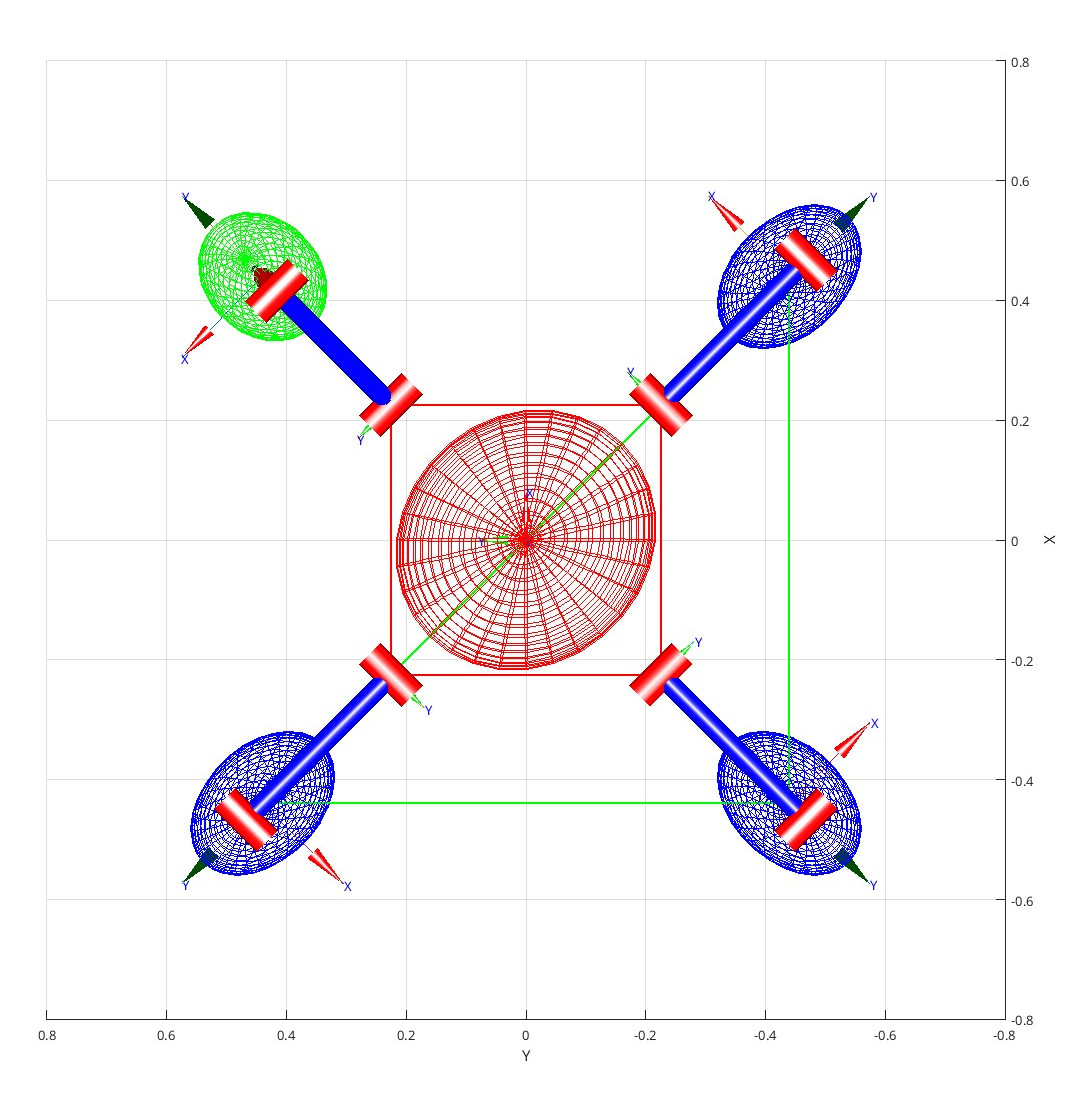
\includegraphics[width=0.35\textwidth]{Images/img_ch3/ex1_z01_LFup_xy.jpg}} \\
    \subfloat[z=0.1, x=-0.1, y=-0.1, and LF up, perspective view \label{fig:ex1_z01_xneg01_yneg01_LFup_ortho}]{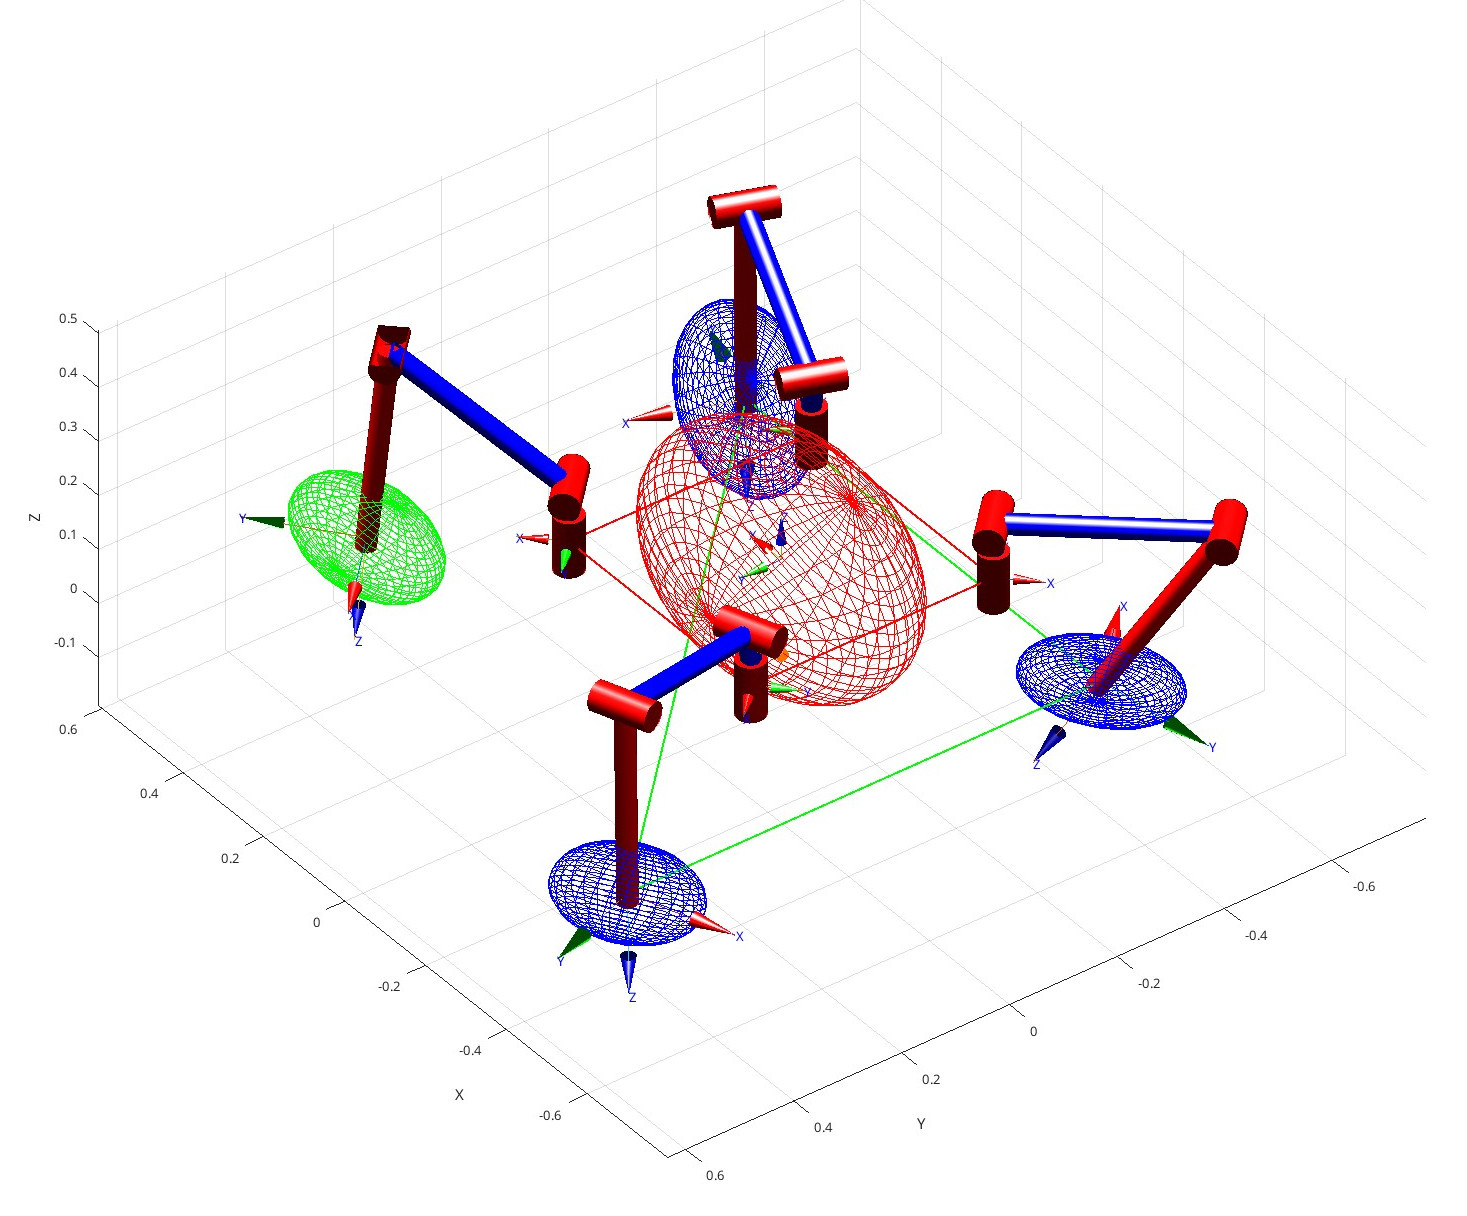
\includegraphics[width=0.35\textwidth]{Images/img_ch3/ex1_z01_xneg01_yneg01_LFup_ortho.jpg}}
    \subfloat[z=0.1, x=-0.1, y=-0.1, and LF up, xy view \label{fig:ex1_z01_xneg01_yneg01_LFup_xy}]{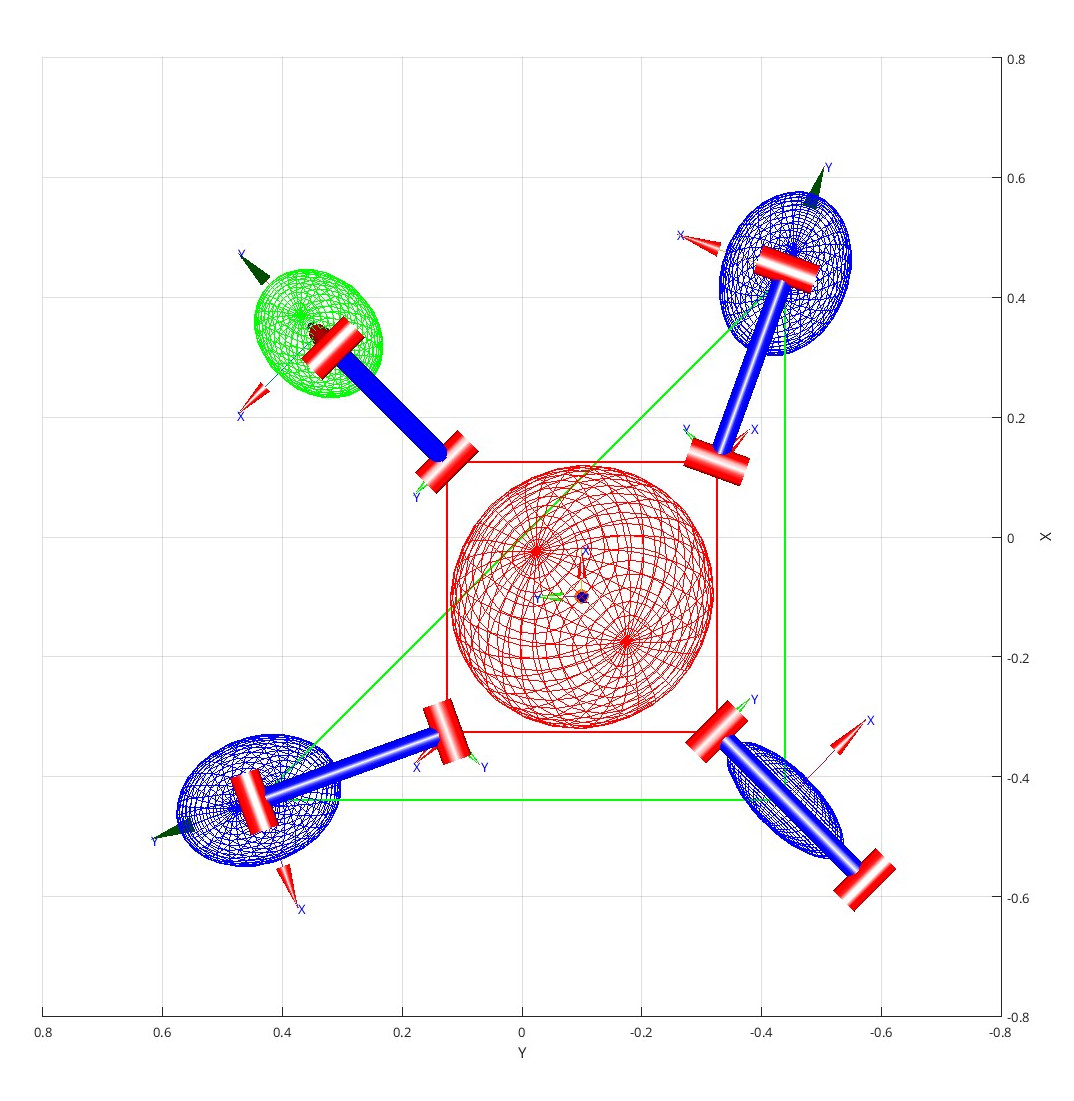
\includegraphics[width=0.35\textwidth]{Images/img_ch3/ex1_z01_xneg01_yneg01_LFup_xy.jpg}} 
    \caption[LimbedEx1 ME after LF limb up and base translation]{LimbedEx1 ME after LF limb up and base translation}
    \label{fig:ex1_rise_limb}
\end{figure}

\subsubsection{Example 2: Hexapod with 3-DOFs Limbs}
\label{sec:BME_hexapod}

This example is an extension of the previous one, to prove that more limbs are not a problem, therefore it is considered a 6-limbed robot with the same limb structure as before (now referred to as LimbedEx2). 
The robot is represented in Fig.\ref{fig:ex2_robot}, with all limbs in the zero configuration $\mathbf{q_0} = \begin{bmatrix}
    0 & 0 & 0
\end{bmatrix}^T$ and in the initial walking configuration $\mathbf{q_W} = \begin{bmatrix}
    0 & -\pi/6 & \frac{2}{3}\pi
\end{bmatrix}^T$.

\begin{figure}[H]
    \centering
    \subfloat[LimbedEx2 with limbs in $\mathbf{q_0}$\label{fig:ex2_q0}]{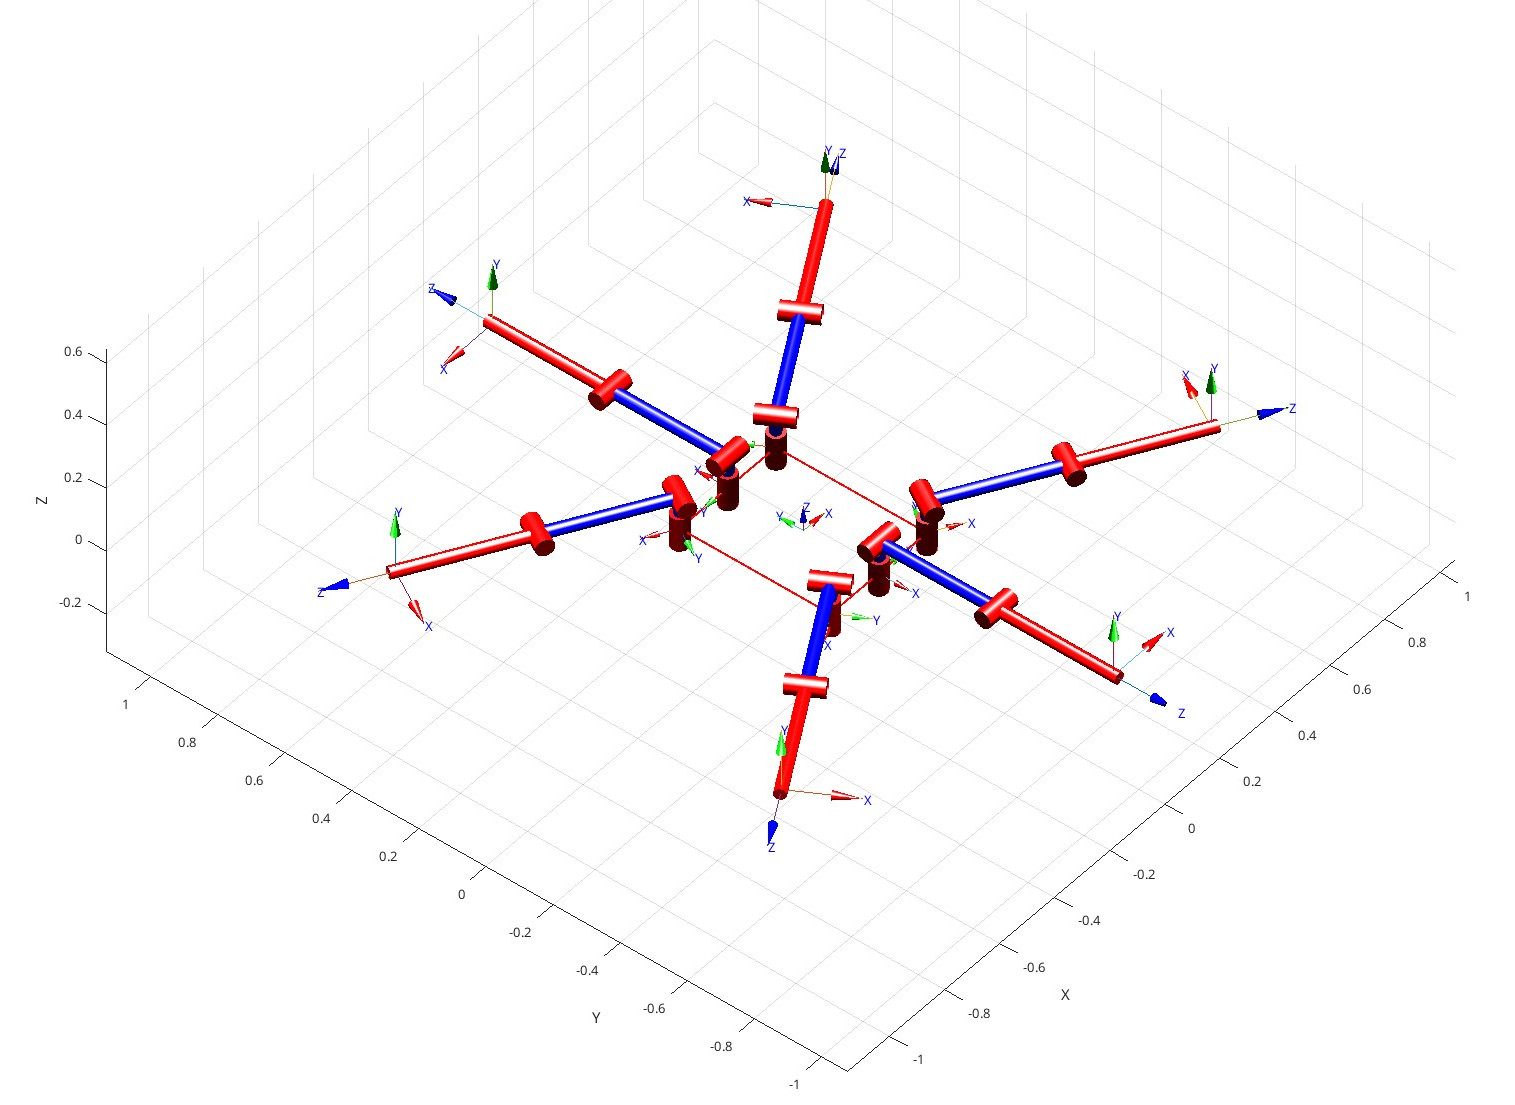
\includegraphics[width=0.45\textwidth]{Images/img_ch3/hexapod_q0.jpg}}
    \subfloat[LimbedEx2 with limbs in $\mathbf{q_W}$\label{fig:ex2_qw}]{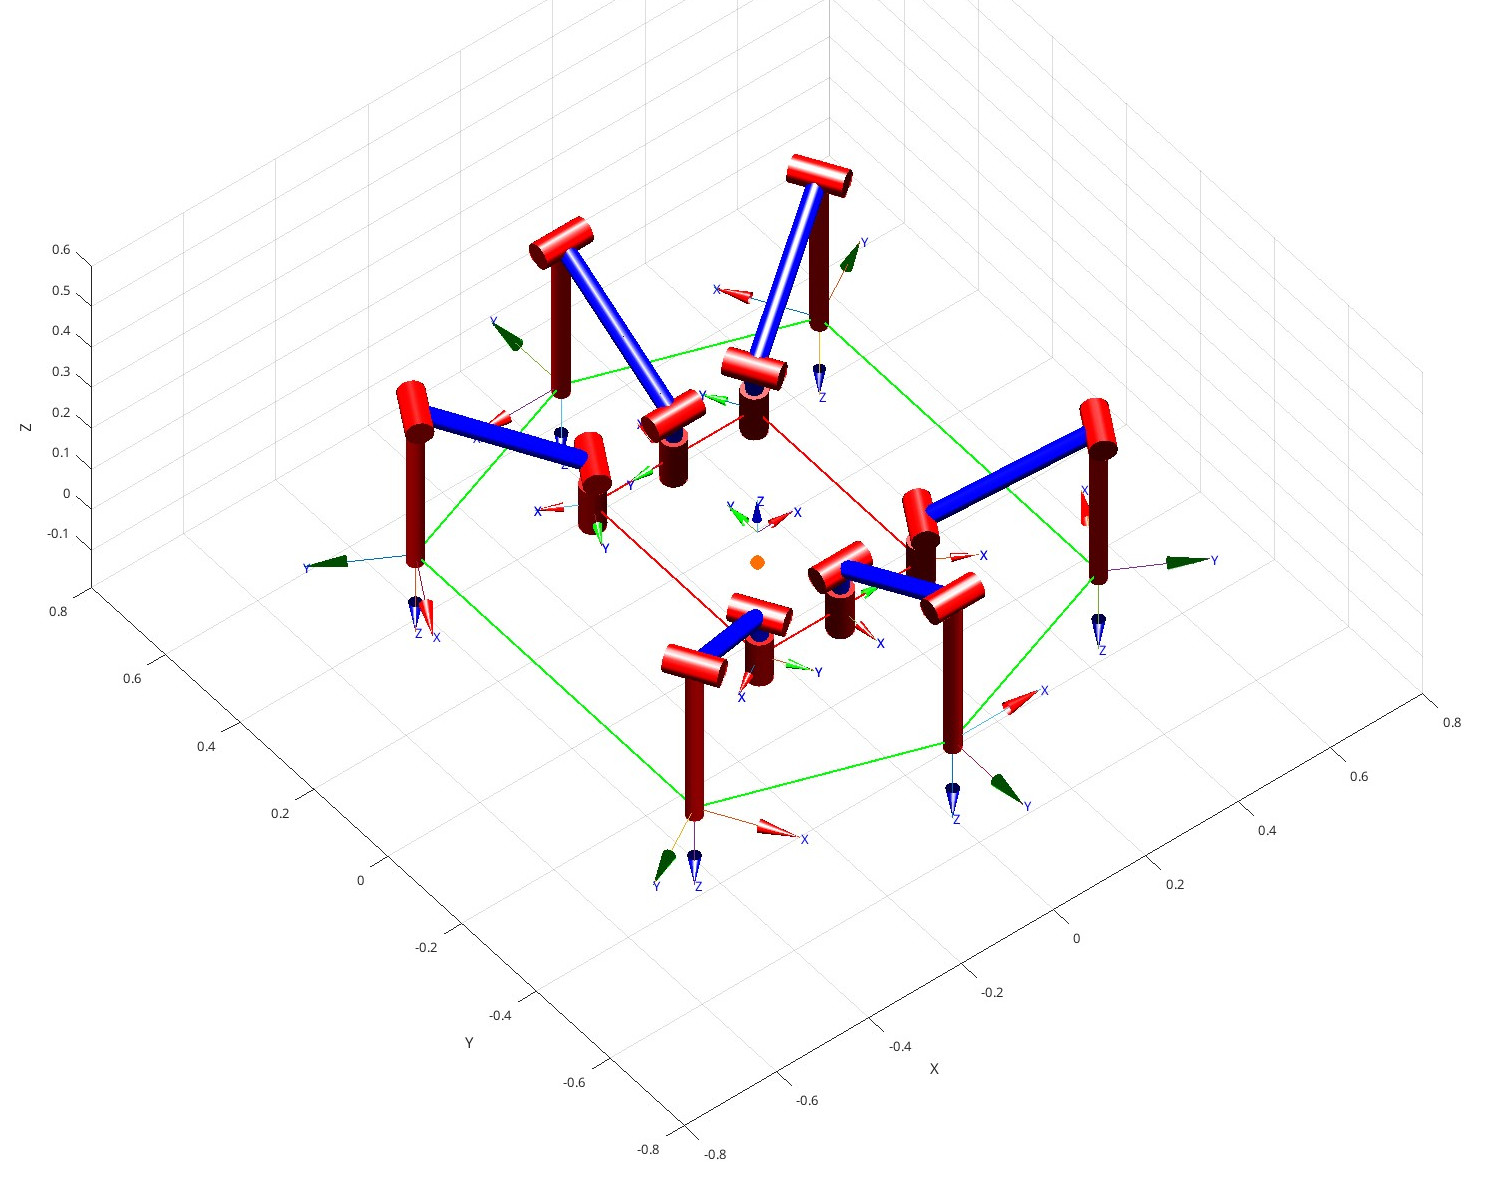
\includegraphics[width=0.45\textwidth]{Images/img_ch3/hexapod_qw.jpg}} 
    \caption[LimbedEx2 in zero and walking configuration]{LimbedEx2 in zero and walking configuration}
    \label{fig:ex2_robot}
\end{figure}

 Similarly to example 1, configurations computed as base motion from the walking one can be tested to evaluate the validity of the ATBVME for multi-limbed robots. The results obtained from the analysis of the ellipsoid shape and volume are the same as the previous example, with the same limitation in the unexpectedly increasing volume.  
 
\textbf{Walking Configuration}
\begin{figure}[H]
    \centering
    \subfloat[perspective view\label{fig:ex2_walking_ortho}]{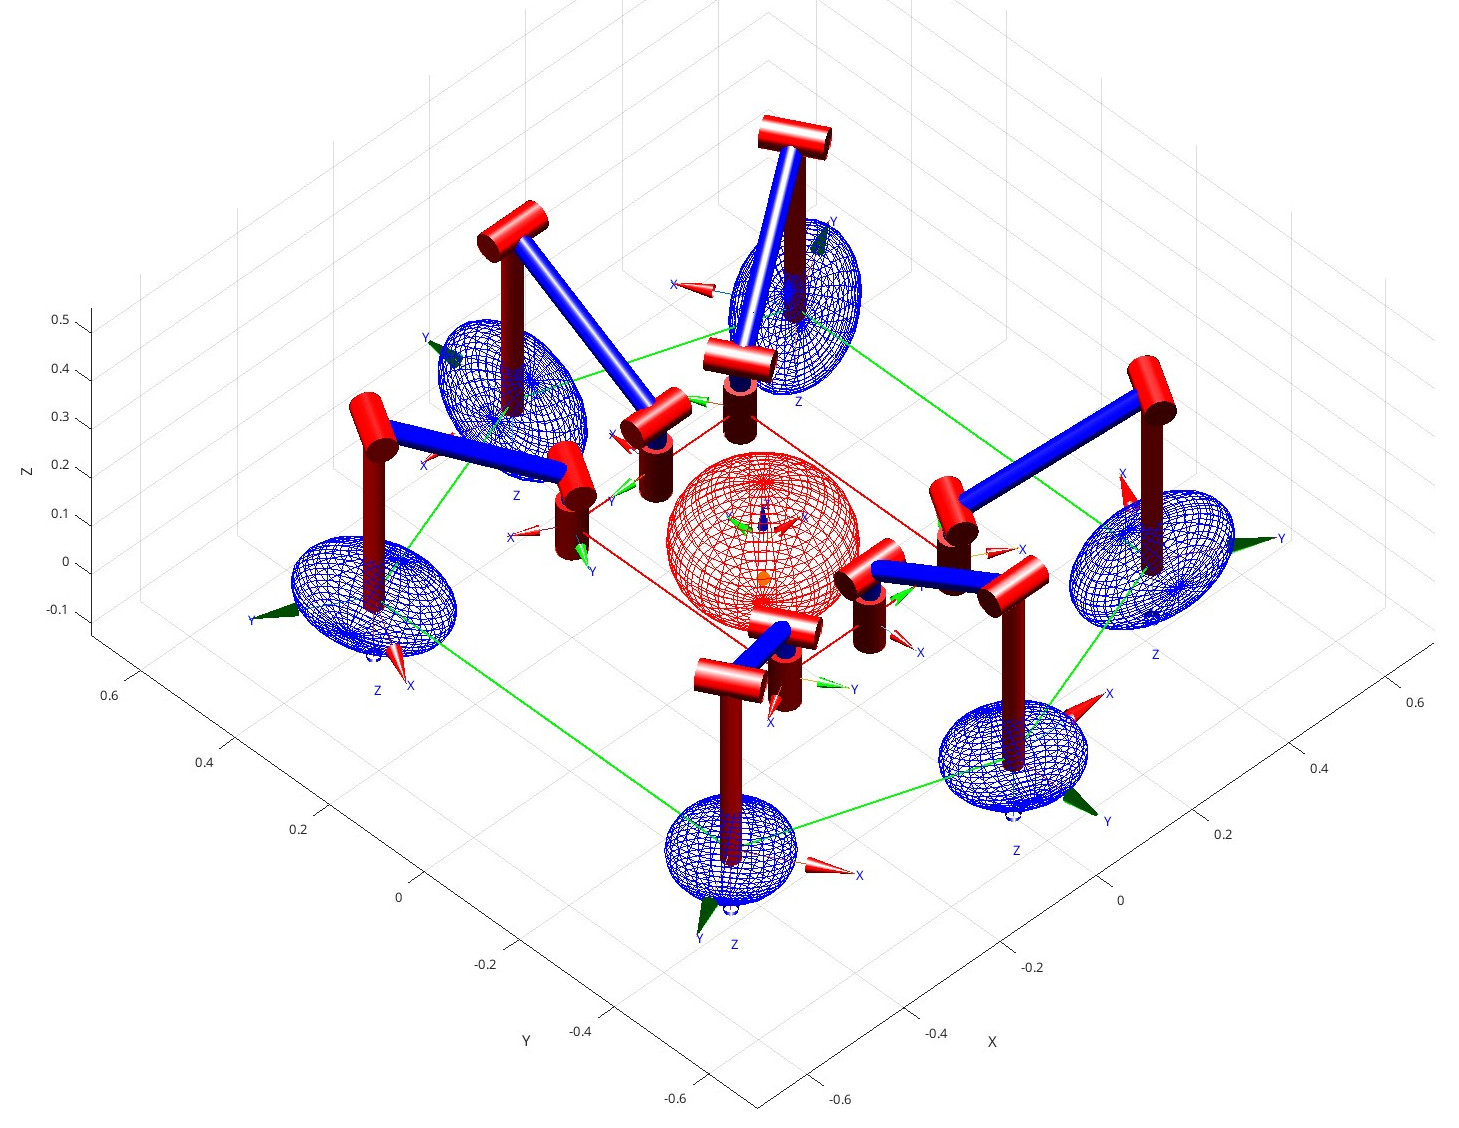
\includegraphics[width=0.3\textwidth]{Images/img_ch3/ex2_walking_ortho.jpg}}
    \subfloat[xy view\label{fig:ex2_walking_xy}]{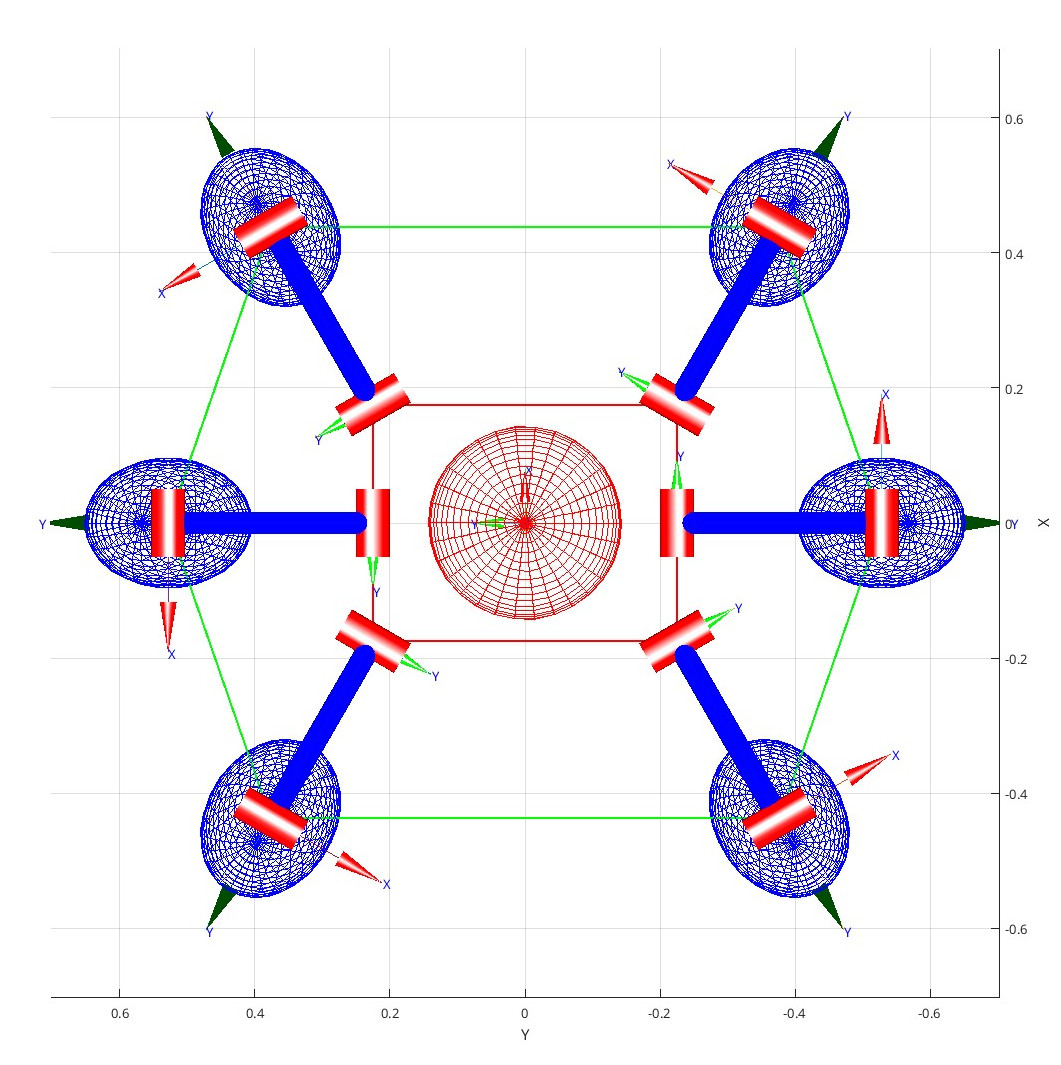
\includegraphics[width=0.3\textwidth]{Images/img_ch3/ex2_walking_xy.jpg}} 
    \subfloat[xz view\label{fig:ex2_walking_xz}]
    {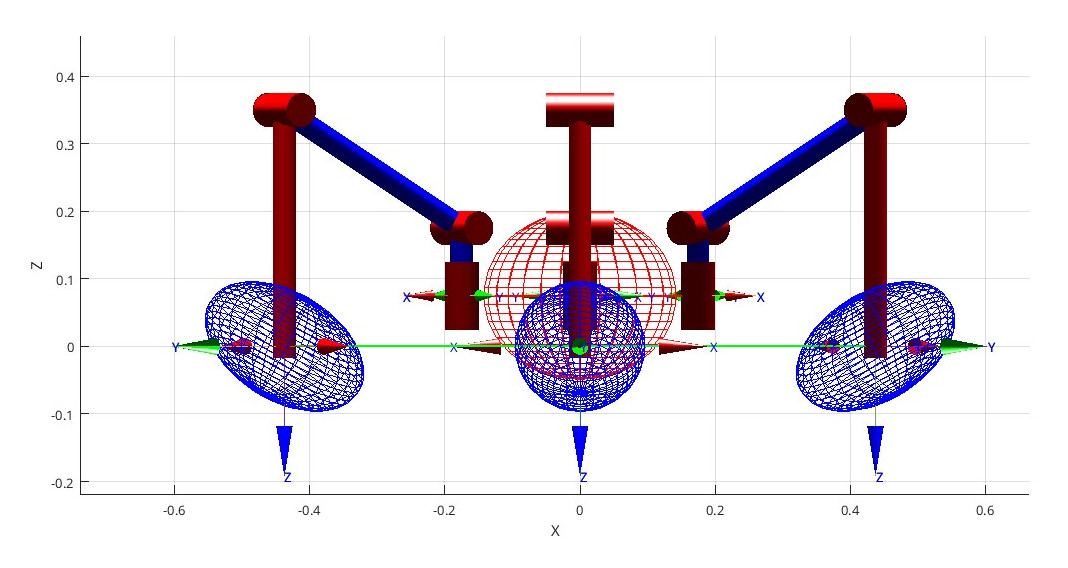
\includegraphics[width=0.3\textwidth]{Images/img_ch3/ex2_walking_xz.jpg}} 
    \caption[LimbedEx2 ME in walking configuration]{LimbedEx2 ME in walking configuration}
    \label{fig:ex2_walking}
\end{figure}
\newpage
\textbf{Base z translations}
\begin{figure}[H]
    \centering
    \subfloat[z=0.2, perspective view\label{fig:ex2_z020_xy}]{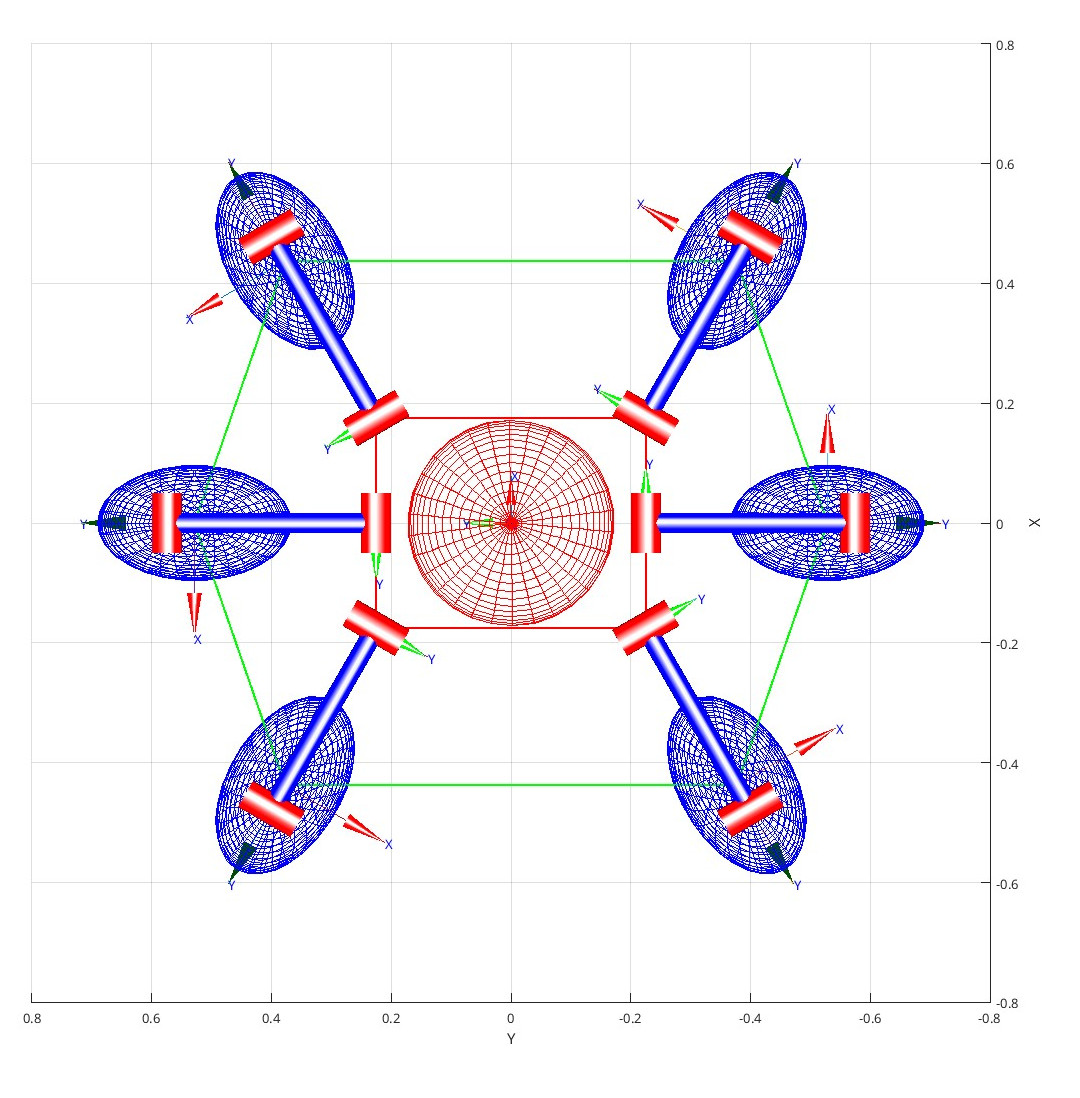
\includegraphics[width=0.35\textwidth]{Images/img_ch3/ex2_z020_xy.jpg}}
    \subfloat[z=0.2, xy view\label{fig:ex2_z020_xz}]{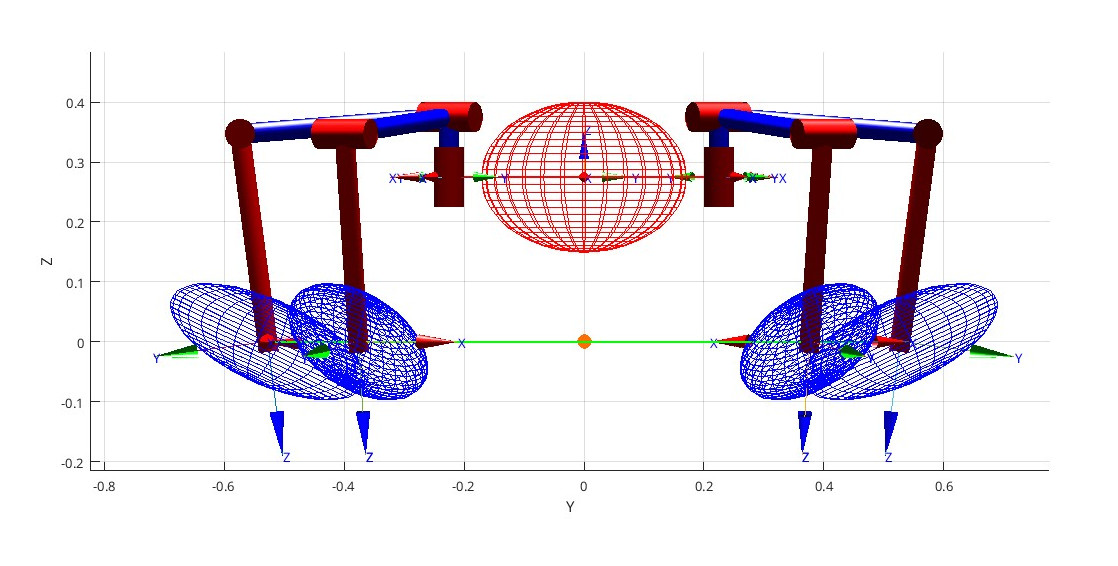
\includegraphics[width=0.35\textwidth]{Images/img_ch3/ex2_z020_xz.jpg}} \\
    \subfloat[z=0.4, xz view\label{fig:ex2_z040_xy}]
    {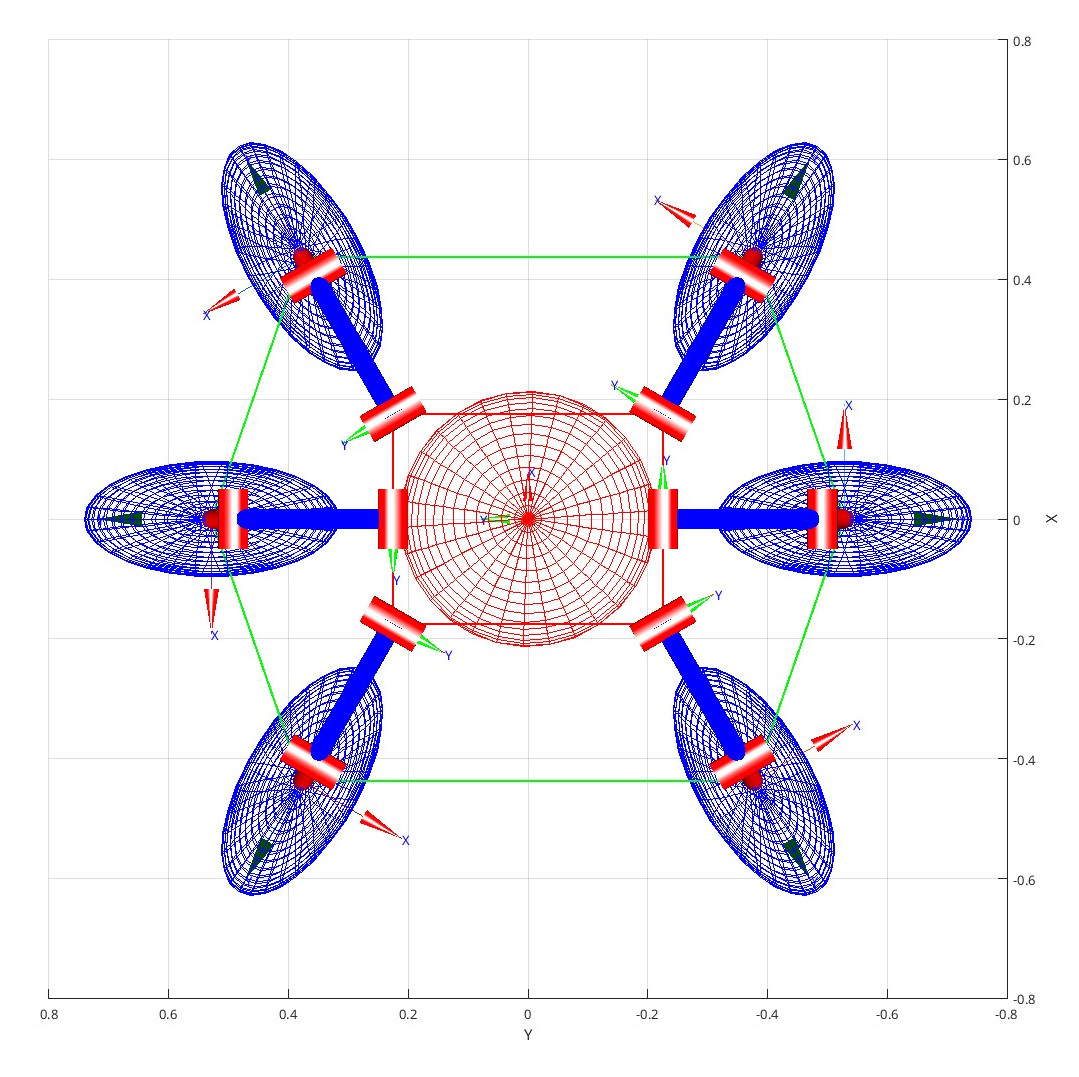
\includegraphics[width=0.35\textwidth]{Images/img_ch3/ex2_z040_xy.jpg}} 
    \subfloat[z=0.4, yz view\label{fig:ex2_z040_yz}]
    {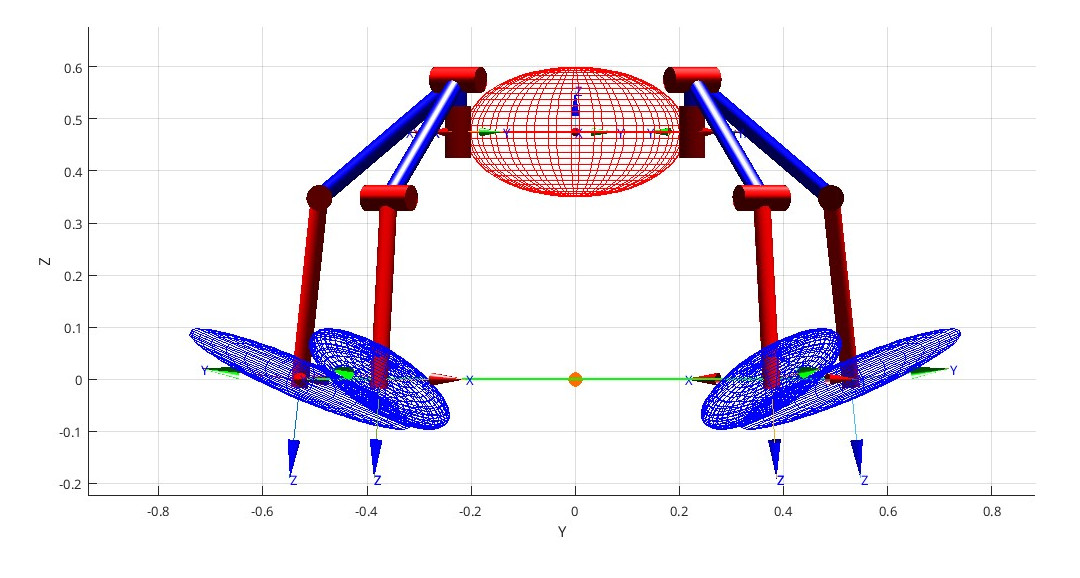
\includegraphics[width=0.35\textwidth]{Images/img_ch3/ex2_z040_yz.jpg}} 
    \caption[LimbedEx2 ME after z base translation]{LimbedEx2 ME after z base translation}
    \label{fig:ex2_z}
\end{figure}

\textbf{Base x,y,z translations}
\begin{figure}[H]
    \centering
    \subfloat[perspective view\label{fig:ex2_xneg02_y01_z015_ortho}]{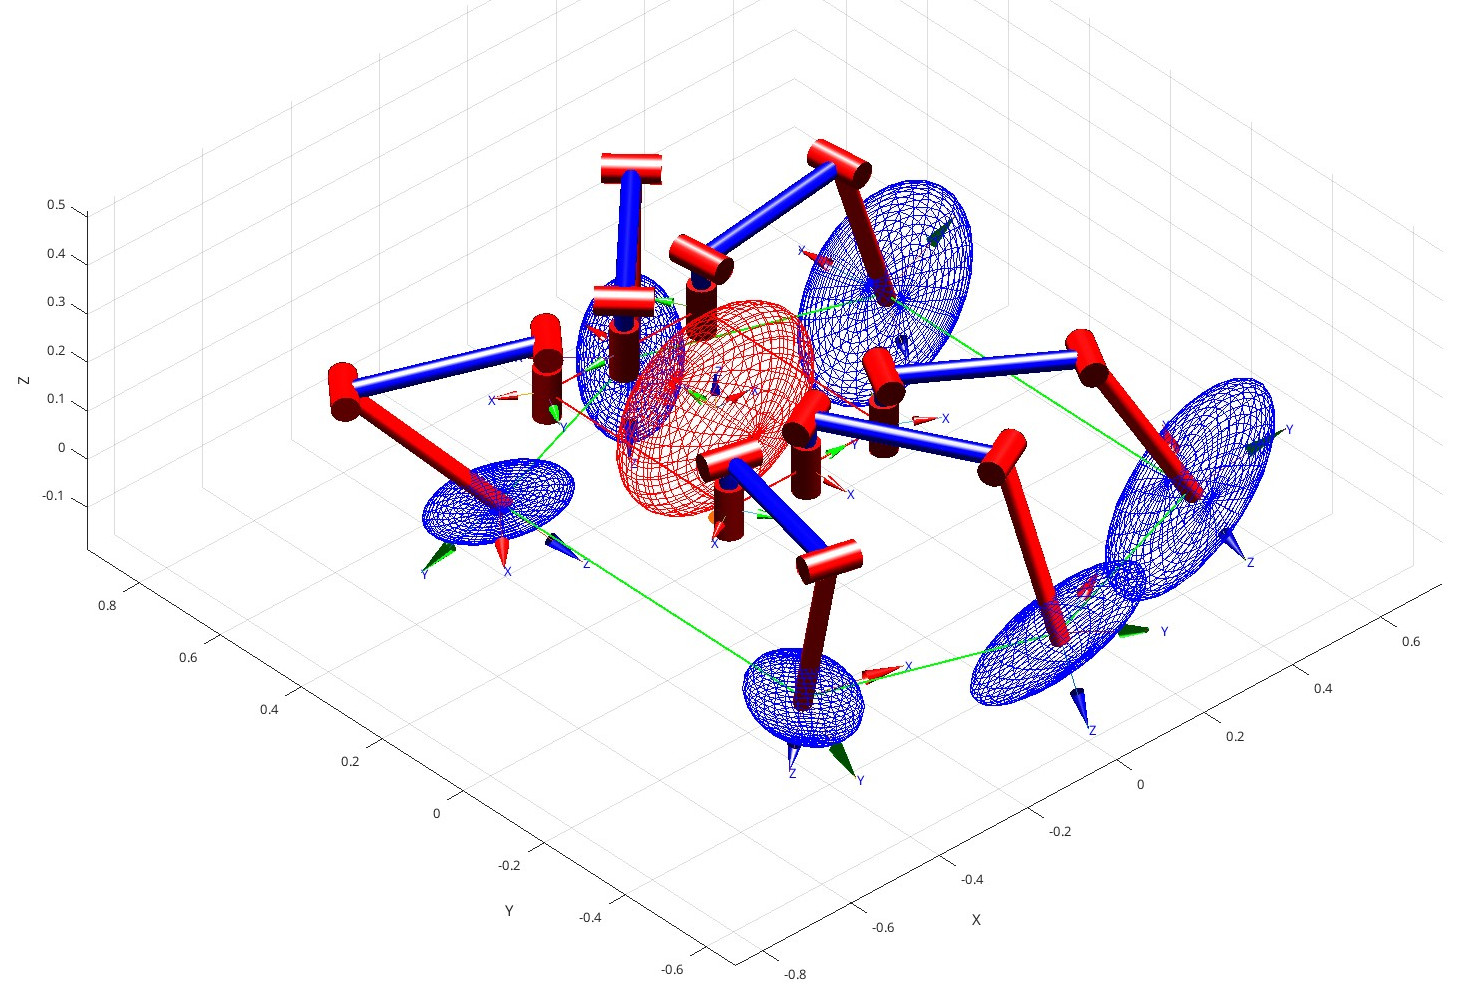
\includegraphics[width=0.3\textwidth]{Images/img_ch3/ex2_xneg02_y01_z015_ortho.jpg}}
    \subfloat[xy view\label{fig:ex2_xneg02_y01_z015_xy}]{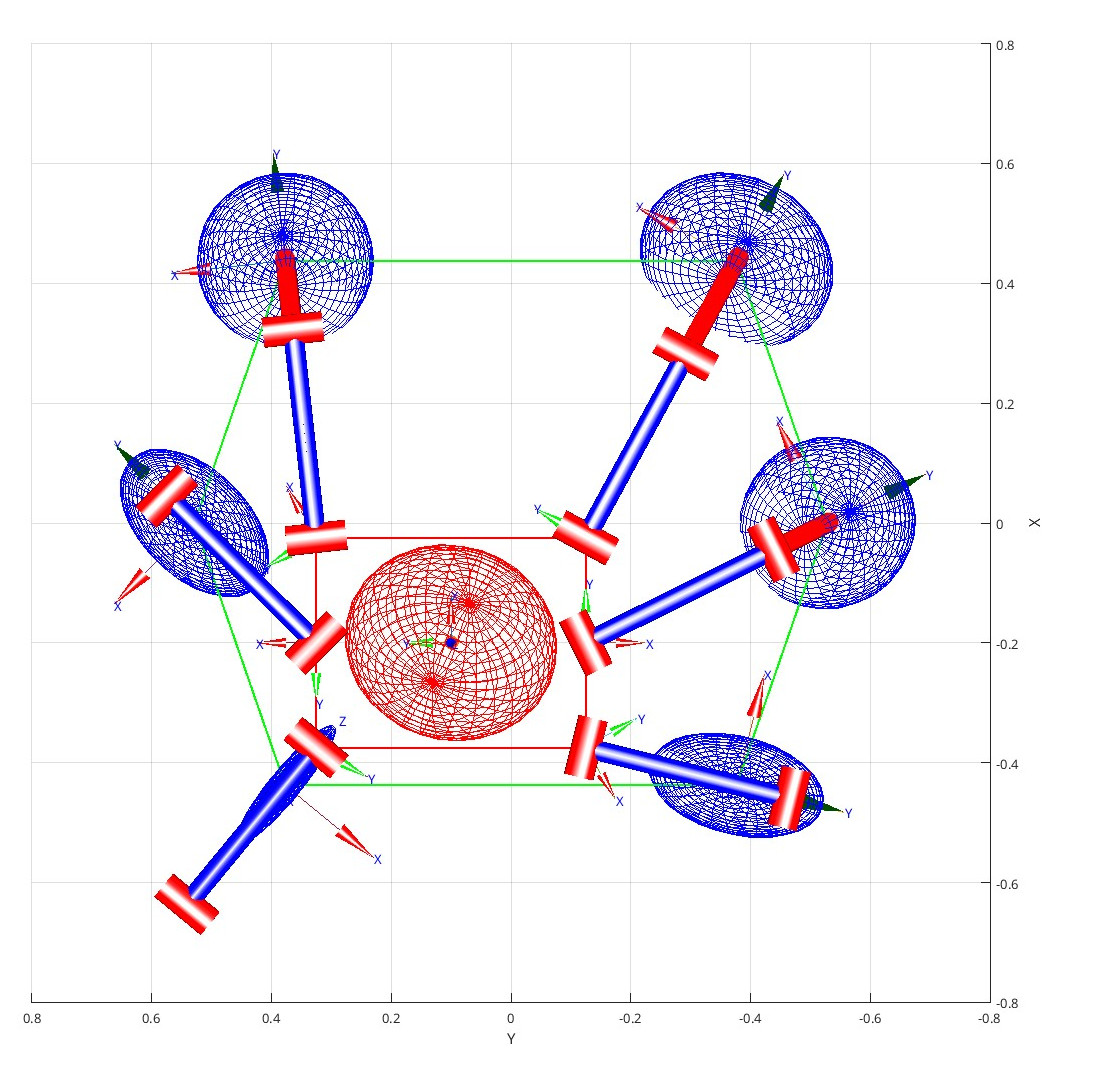
\includegraphics[width=0.3\textwidth]{Images/img_ch3/ex2_xneg02_y01_z015_xy.jpg}} 
    \subfloat[xz view\label{fig:ex2_xneg02_y01_z015_xz}]
    {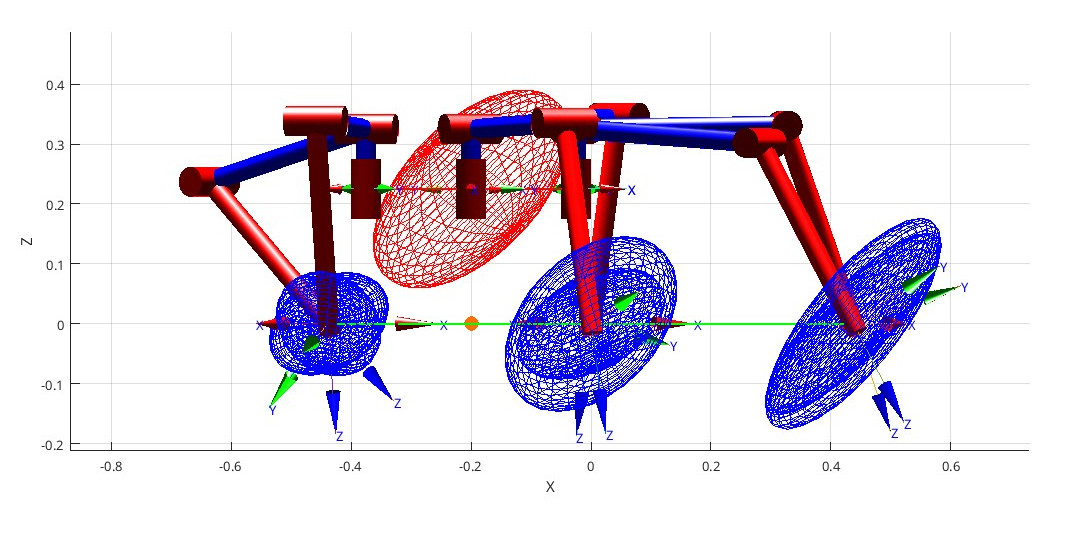
\includegraphics[width=0.3\textwidth]{Images/img_ch3/ex2_xneg02_y01_z015_xz.jpg}} 
    \caption[LimbedEx2 ME after base x=-0.2, y=0.1, z=0.15  translation]{LimbedEx2 ME after base x=-0.2, y=0.1, z=0.15  translation}
    \label{fig:ex2_xyz_translate}
\end{figure}
\newpage
\textbf{Raise Limb}
\begin{figure}[H]
    \centering
    \subfloat[LF and RF up, z=0.15, perspective view \label{fig:ex2_z015_LFRFUP_ortho}]{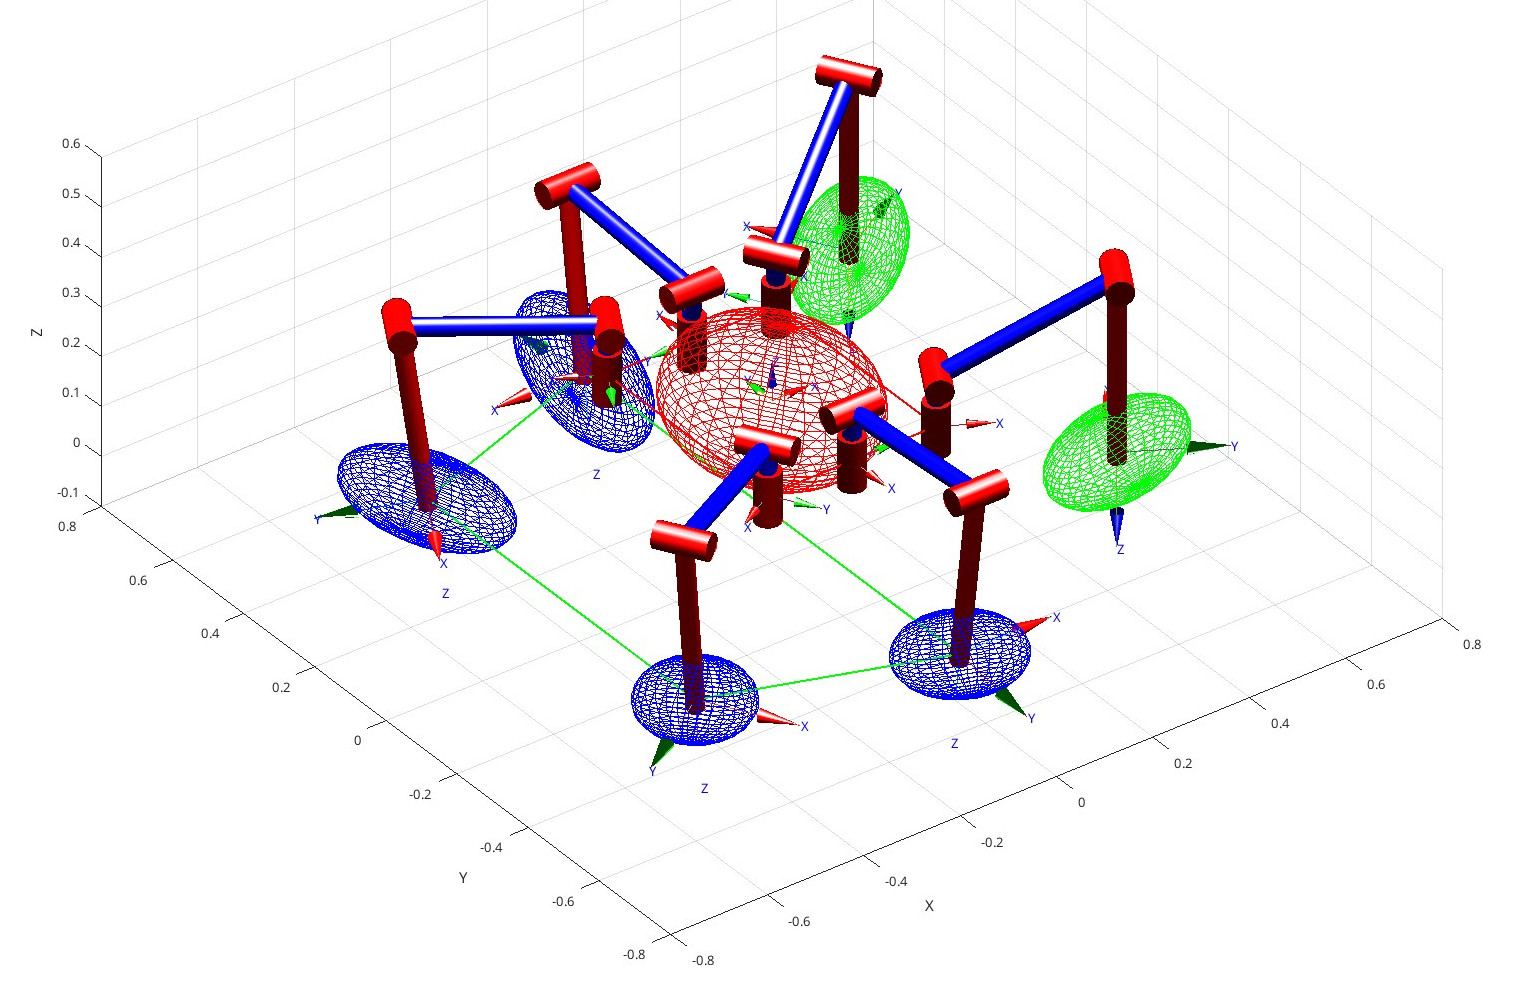
\includegraphics[width=0.45\textwidth]{Images/img_ch3/ex2_z015_LFRFUP_ortho.jpg}}
    \subfloat[LF and RF up, z=0.15,  xz view \label{fig:ex2_z015_LFRFUP_xz}]{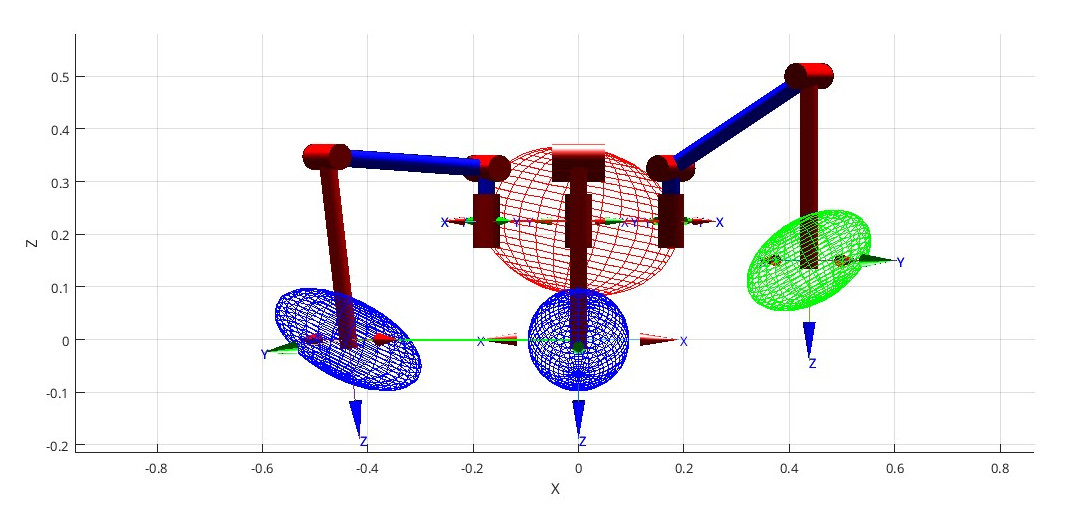
\includegraphics[width=0.45\textwidth]{Images/img_ch3/ex2_z015_LFRFUP_xz.jpg}} \\
    \subfloat[LF and RF up, z=0.15, x=-0.2, perspective view \label{fig:ex2_z015_xneg02_LFRFUP_ortho}]{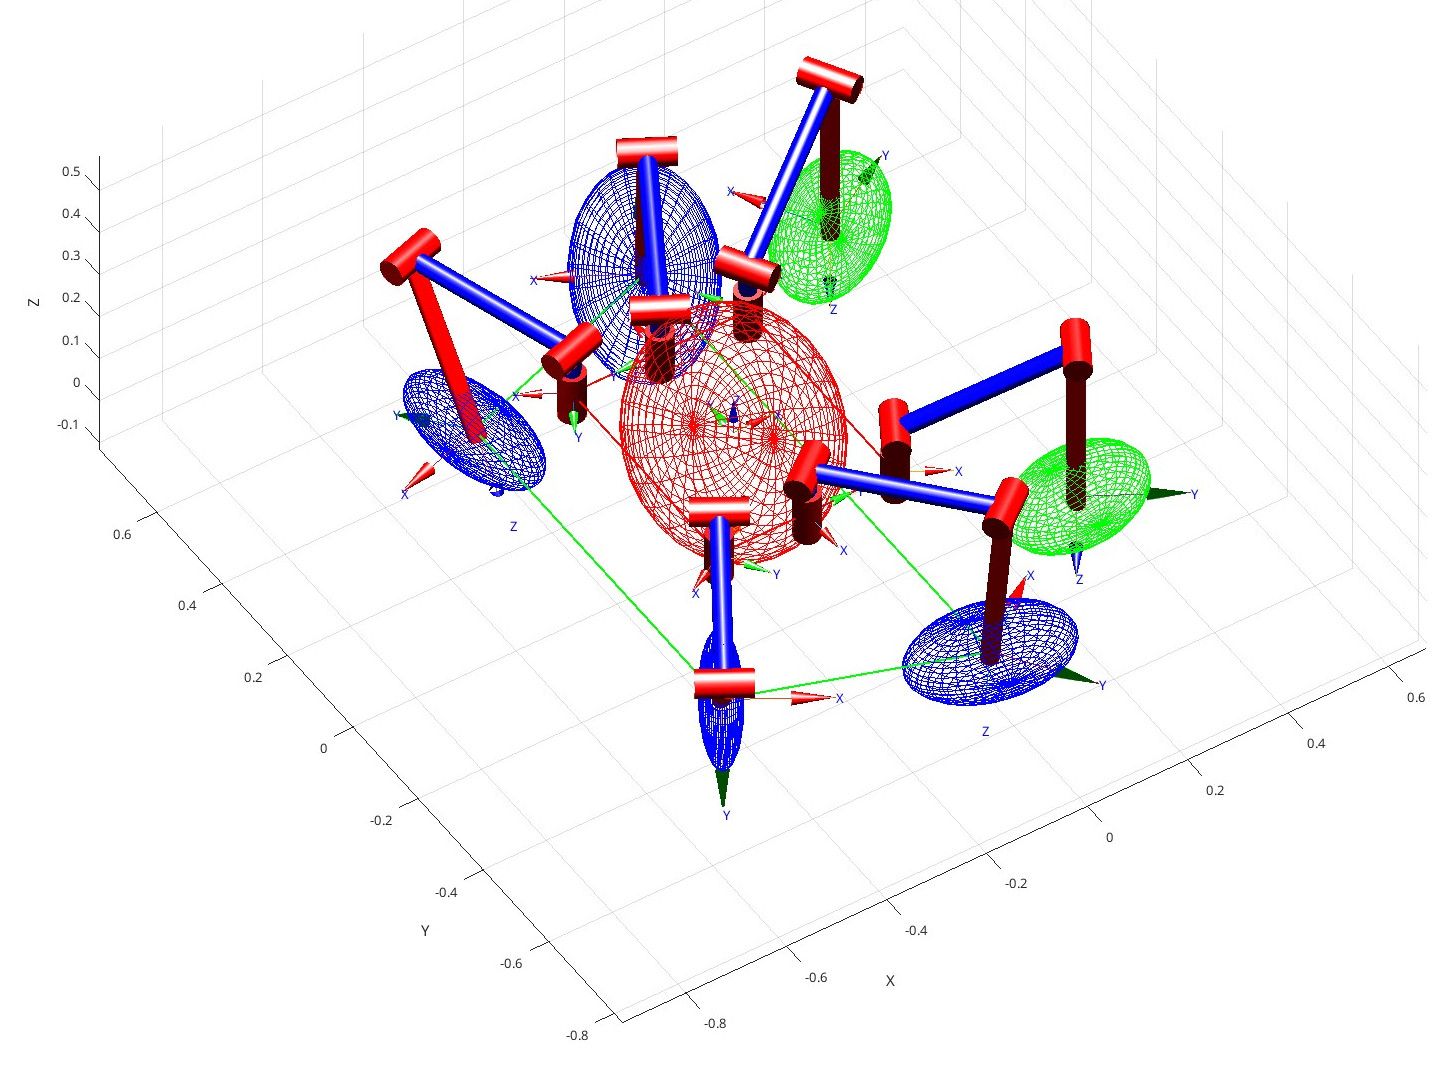
\includegraphics[width=0.45\textwidth]{Images/img_ch3/ex2_z015_xneg02_LFRFUP_ortho.jpg}}
    \subfloat[LF and RF up, z=0.15, x=-0.2, xz view \label{fig:ex2_z015_xneg02_LFRFUP_xz}]{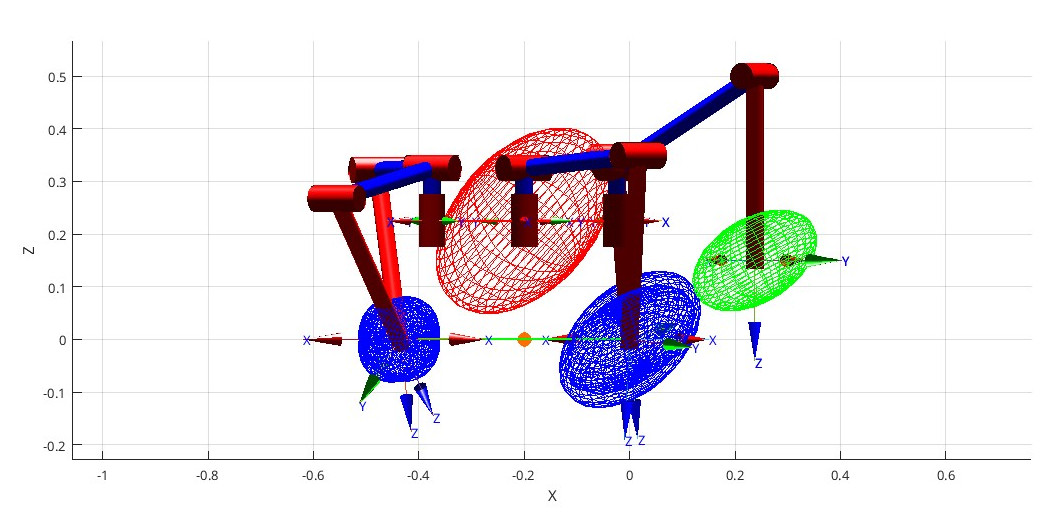
\includegraphics[width=0.45\textwidth]{Images/img_ch3/ex2_z015_xneg02_LFRFUP_xz.jpg}} \\
    \subfloat[LF, LB, RM up, z=0.15, perspective view \label{fig:ex2_z015_LFLBRMUP_ortho}]{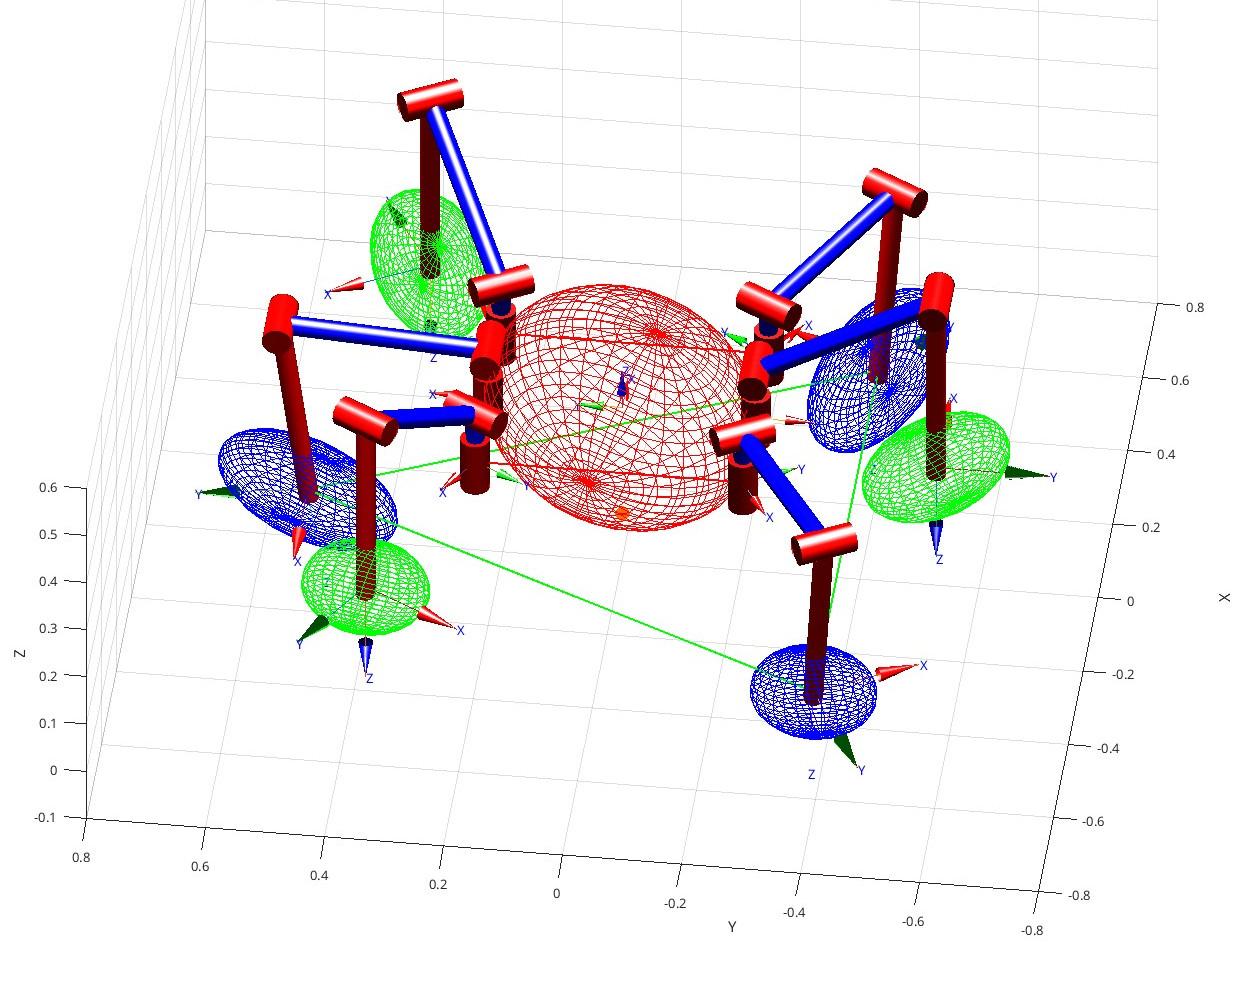
\includegraphics[width=0.45\textwidth]{Images/img_ch3/ex2_z015_LFLBRMUP_ortho.jpg}}
    \subfloat[LF, LB, RM up, z=0.15, yz view \label{fig:ex2_z015_LFLBRMUP_yz}]{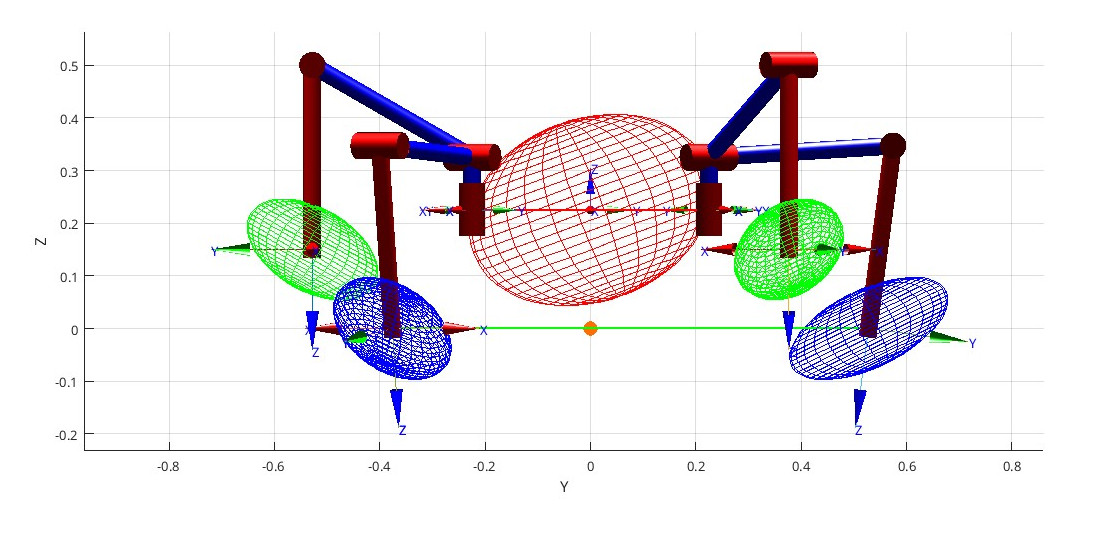
\includegraphics[width=0.45\textwidth]{Images/img_ch3/ex2_z015_LFLBRMUP_yz.jpg}}
    \caption[LimbedEx2 ME after limbs raise and base translation]{LimbedEx2 ME after limbs raise and base translation}
    \label{fig:ex2_rise_limb}
\end{figure}


\subsection{Biomechanics Examples, the Grasshopper}
\label{sec:ME_bio_inspired}

A final example is described in this section, in this case, a common approach to prove the validity of novel theory is used, and biomechanics is considered.

It is common practice to take inspiration from nature\cite{Biomimetics}, and walking robots themselves come from studies on animals' anatomy and gaits\cite{Todd}.
One of the fields of biological sciences is 
Biomechanics, which studies biological systems in their structures, functions, and working principles, and it provides useful insights for bio-inspired engineering solutions. 

It is possible to rely on biomechanical analysis in the opposite direction, proving that a mathematical theory is meaningful because it is coherent with nature. 

For example, applying the manipulability ellipsoid theory of T.Yoshikawa\cite{ManipulabilityYoshikawa} on a reduced human arm model, intuitive results can be found\cite{Siciliano}.

In the same way, here the BME theory is used to analyze the biomechanics of a grasshopper (as the one in Fig.\ref{fig:grasshopper_real}), and if the theory is meaningful results consistent with real documented behavior have to be found. 
The choice of this animal is motivated by its ability to jump, and the particular rear legs configuration taken in preparation for jumping, which inspired different robotic studies and actuation mechanism
\cite{Grasshopper1}\cite{Grasshopper2}\cite{Grasshopper3}.

\begin{figure}[H]
    \centering
    \subfloat[Grasshopper picture\label{fig:grasshopper_real}]{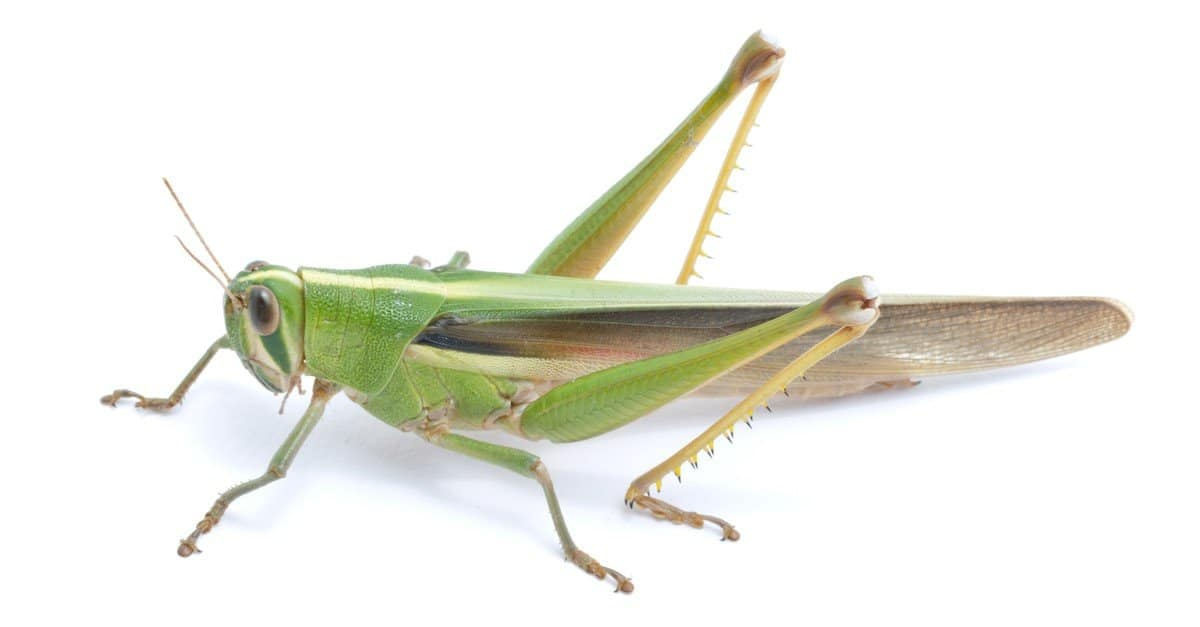
\includegraphics[width=0.4\textwidth]{Images/img_ch3/grasshopper_real.jpg}}\quad
    \subfloat[\cite{Grasshopper3}Anatomic scheme and measurements \label{fig:grasshopper_schema}]{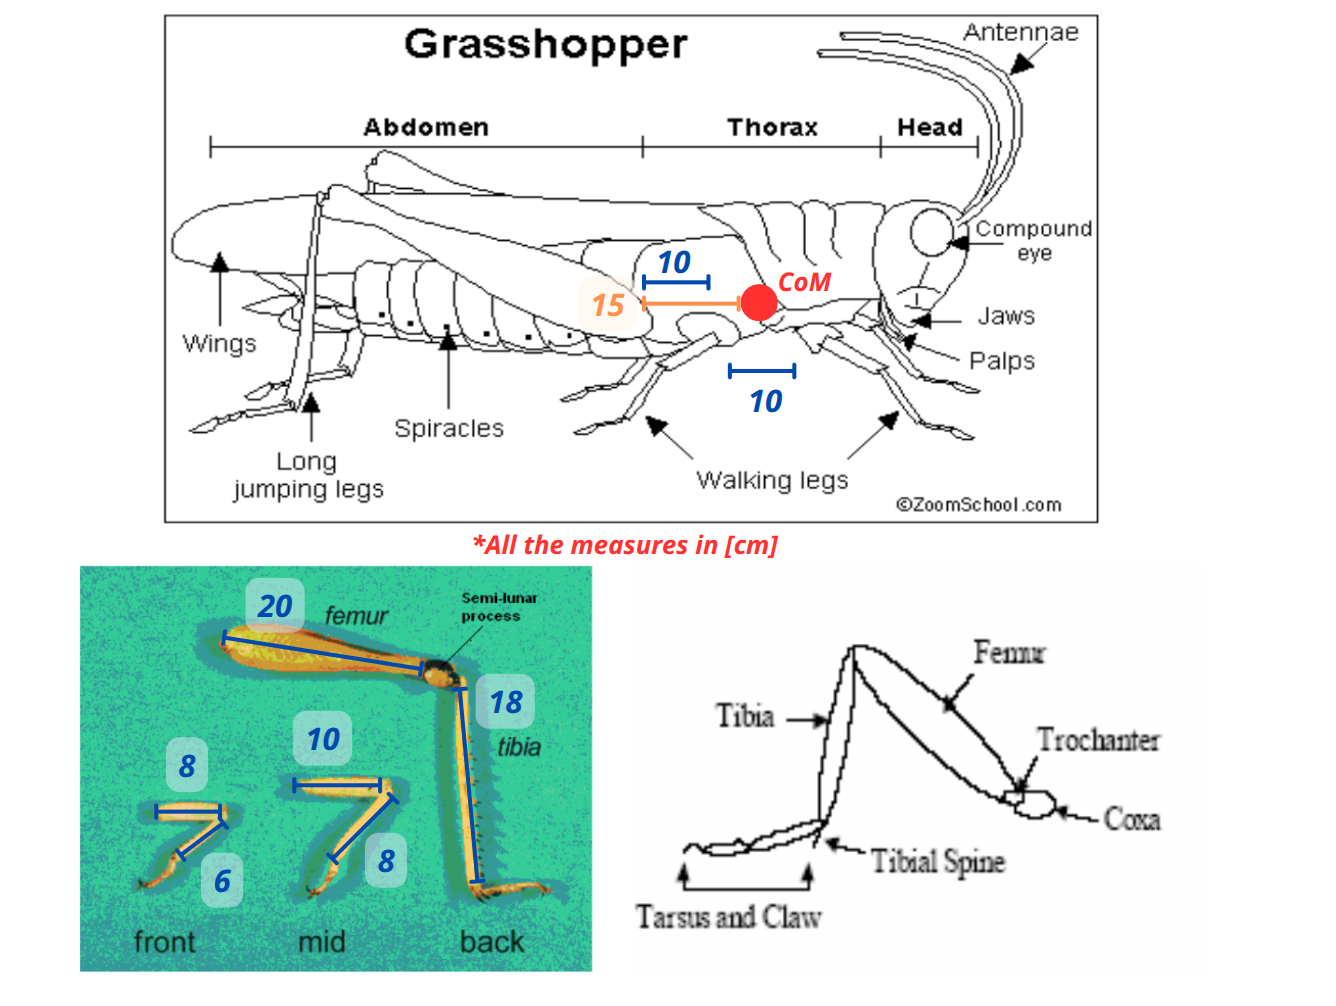
\includegraphics[width=0.55\textwidth]{Images/img_ch3/grasshopper_schema.png}} 
    \caption[Grasshopper picture and anatomic table]{Grasshopper picture and measurements}
    \label{fig:grasshopper}
\end{figure}

The jump is characterized by a big instantaneous body velocity when releasing the rear legs (due to particular leg anatomical features). 
If the BME works, in the jumping configuration the ATBVME should be oriented and elongated in the direction of the jump. 

Furthermore, if one of the rear legs is considered unusable, the jumping direction is affected, and if both cannot be used, the jumping ability is lost.
Finally, uncommon hind leg configurations and unrealistic body CoM locations are tested, to verify the consequence. 

First, an approximated kinematic model of the relevant DOFs of the legs (front, mid, and back) is derived.
The "approximation" neglects the additional links and joints used by the animal for additional mobility, not fundamental in the current analysis. 
The used dimensions of all leg links\cite{Grasshopper3} and the distance between them are reported in Fig.\ref{fig:grasshopper_schema}.

The model used for the legs is again the anthropomorphic arm, as the one in figure \ref{fig:antropomorphicDH} of the previous example. With this model, it is possible to represent the relevant joint and frames for this analysis. 
the DH parameters of all the legs models are reported in Tab.\ref{table:grasshopper_DH}.

\begin{table}[H]
\centering 
    \caption{Grasshopper legs DH parameters}
    \begin{tabular}{ c }
    \textbf{Front Legs parameters}
    \end{tabular}
    \begin{tabular}{| c | c | c | c | c | c |}
    \hline
    \rowcolor{bluepoli!40}
%    \rowcolor{bluepoli!40}
     \textbf{Link} &  $a_i$ $[m]$ & $\alpha_i$ $[rad]$ & $d_i$ $[m] $ & $\theta_i$ $[rad]$ & $\theta_{offset, i}$ $[rad]$ \T\B \\
    \hline \hline
    \textbf{CoxaF} ($i=1$) & 0.0 & $-\frac{\pi}{2}$ & 0.0  & $q_{F1}$  & 0.0 \T\B\\
    \hline 
    \textbf{FemurF} ($i=2$) & 0.08 & 0.0  & 0.0  & $q_{F2}$  & 0.0  \T\B\\
    \hline
    \textbf{TibiaF} ($i=3$) & 0.06  & 0.0  & 0.0  & $q_{F3}$ & 0.0 \T\B\\
    \hline
    \end{tabular}
    \begin{tabular}{ c }
    \\
    \textbf{Mid Legs parameters}
    \end{tabular}
    \begin{tabular}{| c | c | c | c | c | c |}
    \hline
    \rowcolor{bluepoli!40}
%    \rowcolor{bluepoli!40}
     \textbf{Link} &  $a_i$ $[m]$ & $\alpha_i$ $[rad]$ & $d_i$ $[m] $ & $\theta_i$ $[rad]$ & $\theta_{offset, i}$ $[rad]$ \T\B \\
    \hline \hline
    \textbf{CoxaM} ($i=1$) & 0.0 & $-\frac{\pi}{2}$ & 0.0  & $q_{M1}$  & 0.0 \T\B\\
    \hline 
    \textbf{FemurM} ($i=2$) & 0.10 & 0.0  & 0.0  & $q_{M2}$  & 0.0  \T\B\\
    \hline
    \textbf{TibiaM} ($i=3$) & 0.08  & 0.0  & 0.0  & $q_{M3}$ & 0.0 \T\B\\
    \hline
    \end{tabular} 
    \begin{tabular}{ c }
    \\
    \textbf{Back Legs parameters}
    \end{tabular}
    \begin{tabular}{| c | c | c | c | c | c |}
    \hline
    \rowcolor{bluepoli!40}
%    \rowcolor{bluepoli!40}
     \textbf{Link} &  $a_i$ $[m]$ & $\alpha_i$ $[rad]$ & $d_i$ $[m] $ & $\theta_i$ $[rad]$ & $\theta_{offset, i}$ $[rad]$ \T\B \\
    \hline \hline
    \textbf{CoxaB} ($i=1$) & 0.0 & $-\frac{\pi}{2}$ & 0.0  & $q_{B1}$  & 0.0 \T\B\\
    \hline 
    \textbf{FemurB} ($i=2$) & 0.20 & 0.0  & 0.0  & $q_{B2}$  & 0.0  \T\B\\
    \hline
    \textbf{TibiaB} ($i=3$) & 0.18  & 0.0  & 0.0  & $q_{B3}$ & 0.0 \T\B\\
    \hline
    \end{tabular} 
    \label{table:grasshopper_DH}
\end{table}

Figure \ref{fig:grasshopper_model} represents the overall kinematic model used in the following analysis, with the legs positioned using the distances reported in Fig.\ref{fig:grasshopper_schema}, and the initial legs orientation around the z-axis (Left Front (LF), Left Mid (LM), Left Back (LB)) is $\gamma_{LF} = \pi/6, \gamma_{LM} = \frac{2}{3}\pi, \gamma_{RB}=\pi$, and symmetric for the right ones: RF, RM, and RB.


\begin{figure}[H]
    \centering
    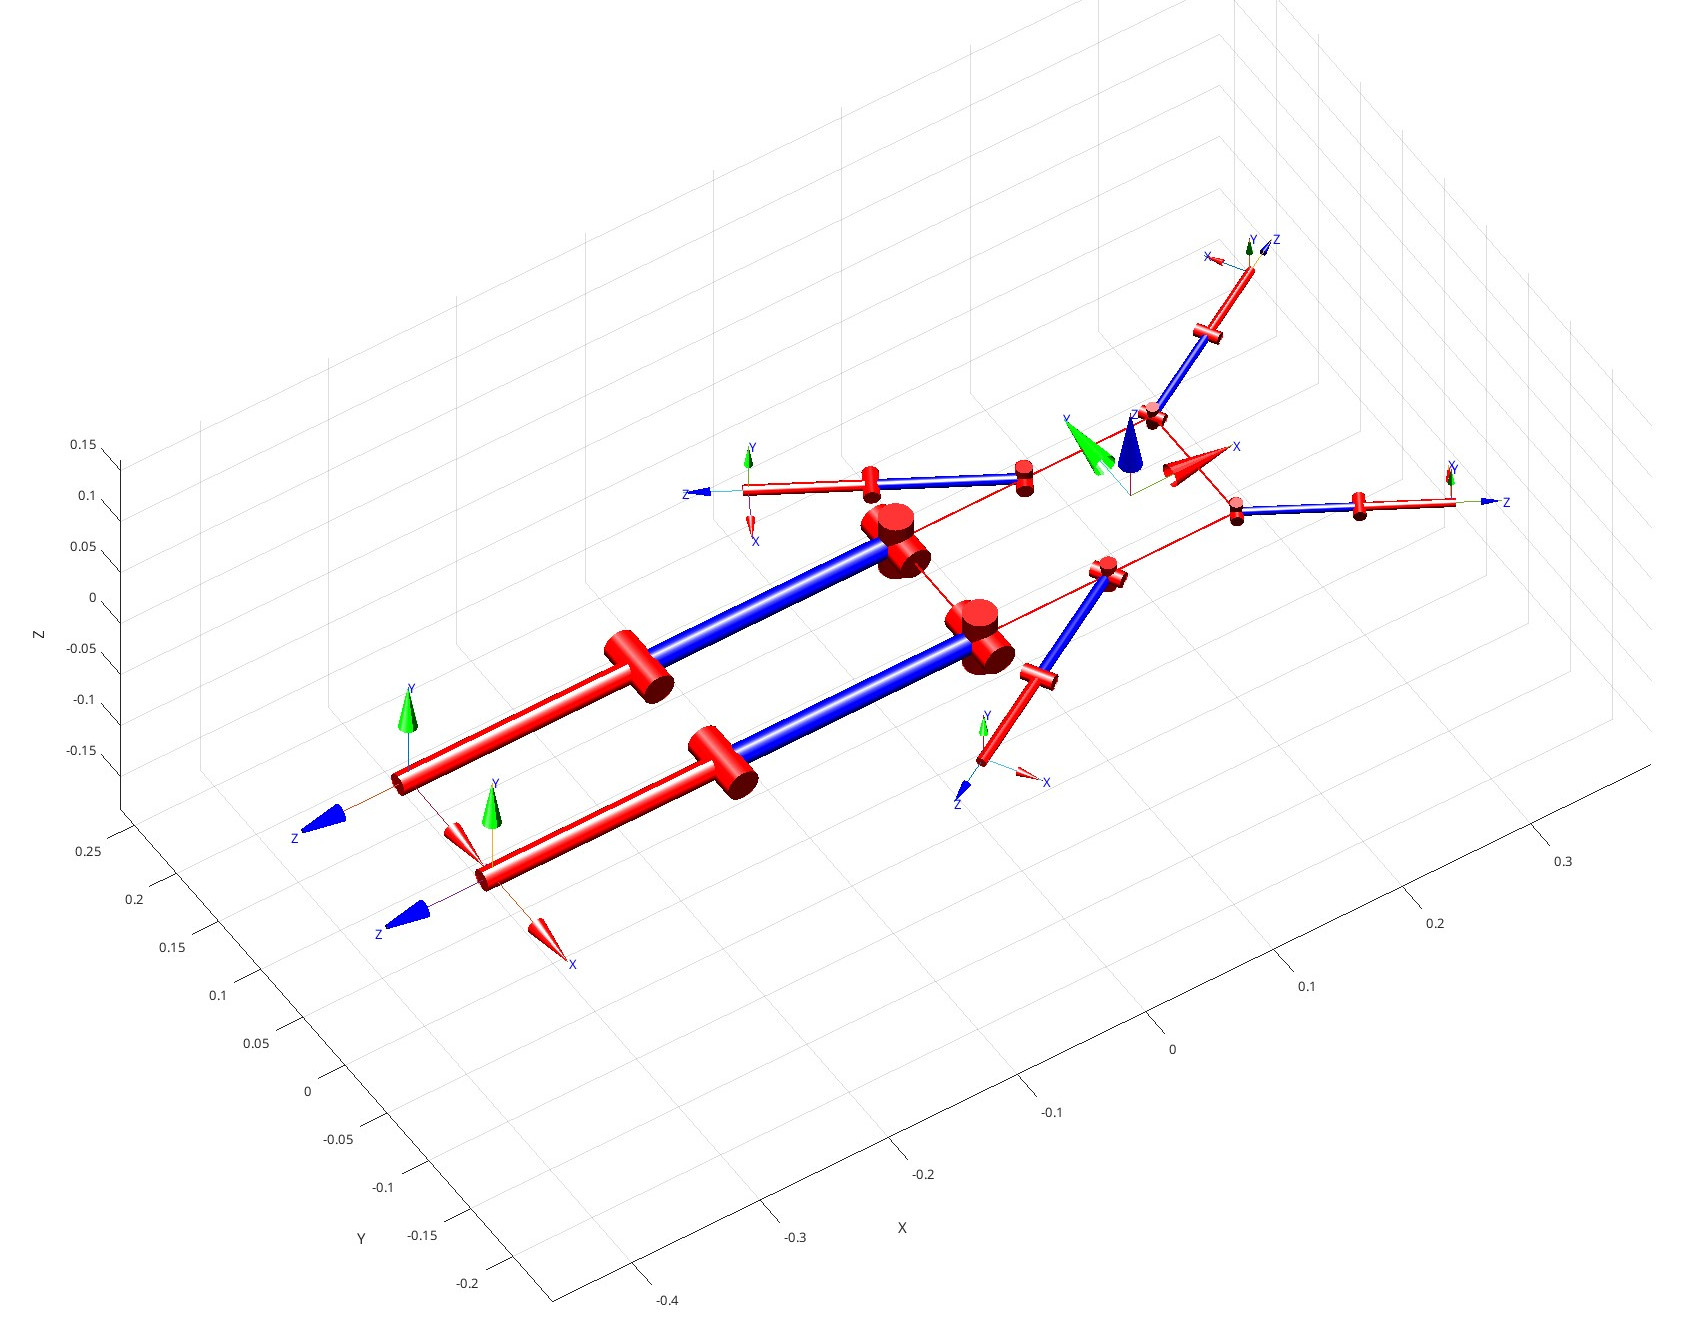
\includegraphics[width=0.7\textwidth]{Images/img_ch3/grasshopper_DH.jpg}
    \caption{Approximated kinematic model of a grasshopper in the zero configuration.}
    \label{fig:grasshopper_model}
\end{figure}

With the model ready to use, the conditions explained before are tested to see if the ATBVME provides meaningful results, in summary the tests are the following: 
\begin{enumerate}
    \setlength\itemsep{-0.7em} 
    \item\label{item:grasshopper_test1}\textbf{Jumping configuration}
    \item\label{item:grasshopper_test2}\textbf{Sensitivity analysis of the jumping configuration}
    \item\label{item:grasshopper_test3}\textbf{One back leg unavailable}
    \item\label{item:grasshopper_test4}\textbf{Both back legs unavailable}
    \item\label{item:grasshopper_test5}\textbf{Sensitivity analysis of CoM position}
\end{enumerate}

To conduct those experiments, first, the different joint velocity limits are considered to use a realistic joint space domain. In particular $\mathbf{Q_{lim}}\in\mathbb{R}^{n\times n}$ is defined \cite{DualArmSpaceManipulabilityEllipsoid}as a diagonal matrix containing the joint limit of all the legs. 
To capture the fact that the front(F) and mid(M) legs are less reactive and used for slow walking, while the back(B) leg's femur-to-tibia joint is the one responsible for the explosive jump (so the fastest one), this aspect is mdeled by defining the limits as:\\
$\mathbf{\dot{q}}_{lim,LF} = \begin{bmatrix}
    0.8 & 0.8 & 0.8
\end{bmatrix}$; 
$\mathbf{\dot{q}}_{lim,LM} = \begin{bmatrix}
    0.8 & 0.8 & 0.8
\end{bmatrix}$; 
$\mathbf{\dot{q}}_{lim,LB} =  \begin{bmatrix}
    1.0 & 1.0 & 4.0
\end{bmatrix}$\\
(with $\mathbf{\dot{q}}_{lim,LF} = \mathbf{\dot{q}}_{lim,RF}$,$\mathbf{\dot{q}}_{lim,LM} = \mathbf{\dot{q}}_{lim,RM}$, $\mathbf{\dot{q}}_{lim,LB} = \mathbf{\dot{q}}_{lim,RB}$)\\

and finally:
$\mathbf{Q}_{lim} = diag(\mathbf{q}_{lim,LF}, \mathbf{q}_{lim,LM}, \mathbf{q}_{lim,LB}, \mathbf{q}_{lim,RF}, \mathbf{q}_{lim,RM}, \mathbf{q}_{lim,RB})$


 because the manipulability theory is relevant to derive the preferred directions rather than the specific numbers\cite{LimitsEllipsoid}, the specific numeric value is not important. Furthermore, this analysis is not rigorous in the exact sizes and dimensions. The important aspect of these boundary values is that the femur-to-tibia joint is the biggest, and the others represent realistic behavior. 

From the definition of $\mathbf{Q}_{lim}$ it is possible to redefine the joint-space sphere behind Yoshikawa's theory in a normalized space $\mathbf{\tilde{\dot{q}}} = \mathbf{Q}^{-1}_{lim}\mathbf{\dot{q}}$, as:
\begin{equation} \mathbf{\tilde{\dot{q}}}^T\mathbf{\tilde{\dot{q}}} = 1
    \label{eq:nornalized_space}
\end{equation}

Then it is simple to rewrite all in the joint space and obtain a new quadratic form for the manipulability ellipsoid, including different symmetric joint limits. In this way, it is possible to give more importance to some of the joints rather than others, solving a limitation of the manipulability theory.  

\textbf{1) Jumping Configuration}\\
In this configuration\cite{Grasshopper3}, the legs are considered with the following joint values, as reported in figure \ref{fig:jumping_config} : 

\begin{equation}
    \label{eq:jumping_config}
    \left\{
    \begin{aligned}
           \mathbf{q}_{LF} = \mathbf{q}_{RF}  = \begin{bmatrix}
               0 &-\frac{\pi}{6} & \frac{2}{3}\pi 
           \end{bmatrix}^T = \begin{bmatrix}
               0 &-30^\circ & 120^\circ 
           \end{bmatrix}^T 
           \\
           \mathbf{q}_{LM} = \mathbf{q}_{RM}  = \begin{bmatrix}
               0 &-\frac{\pi}{6} & \frac{2}{3}\pi 
           \end{bmatrix}^T = \begin{bmatrix}
                0 &-30^\circ & 120^\circ
           \end{bmatrix}^T 
            \\
            \mathbf{q}_{LB} = \mathbf{q}_{RB}  = \begin{bmatrix}
               -\frac{\pi}{12} &-\frac{7}{36}\pi & \frac{8}{9}\pi 
           \end{bmatrix}^T = \begin{bmatrix}
               -15^\circ &-35^\circ & 160^\circ
           \end{bmatrix}^T 
    \end{aligned}
    \right.
\end{equation}

It is evident from the shape of the ATBVME reported in Fig.\ref{fig:jumping_ME_ortho} and \ref{fig:jumping_ME_xz} that a clear jumping direction is indicated by the bigger axis of the ellipsoid, where higher base velocity is achievable. 

\begin{figure}[H]
    \centering
    \subfloat[Jumping configuration\label{fig:jumping_config}]{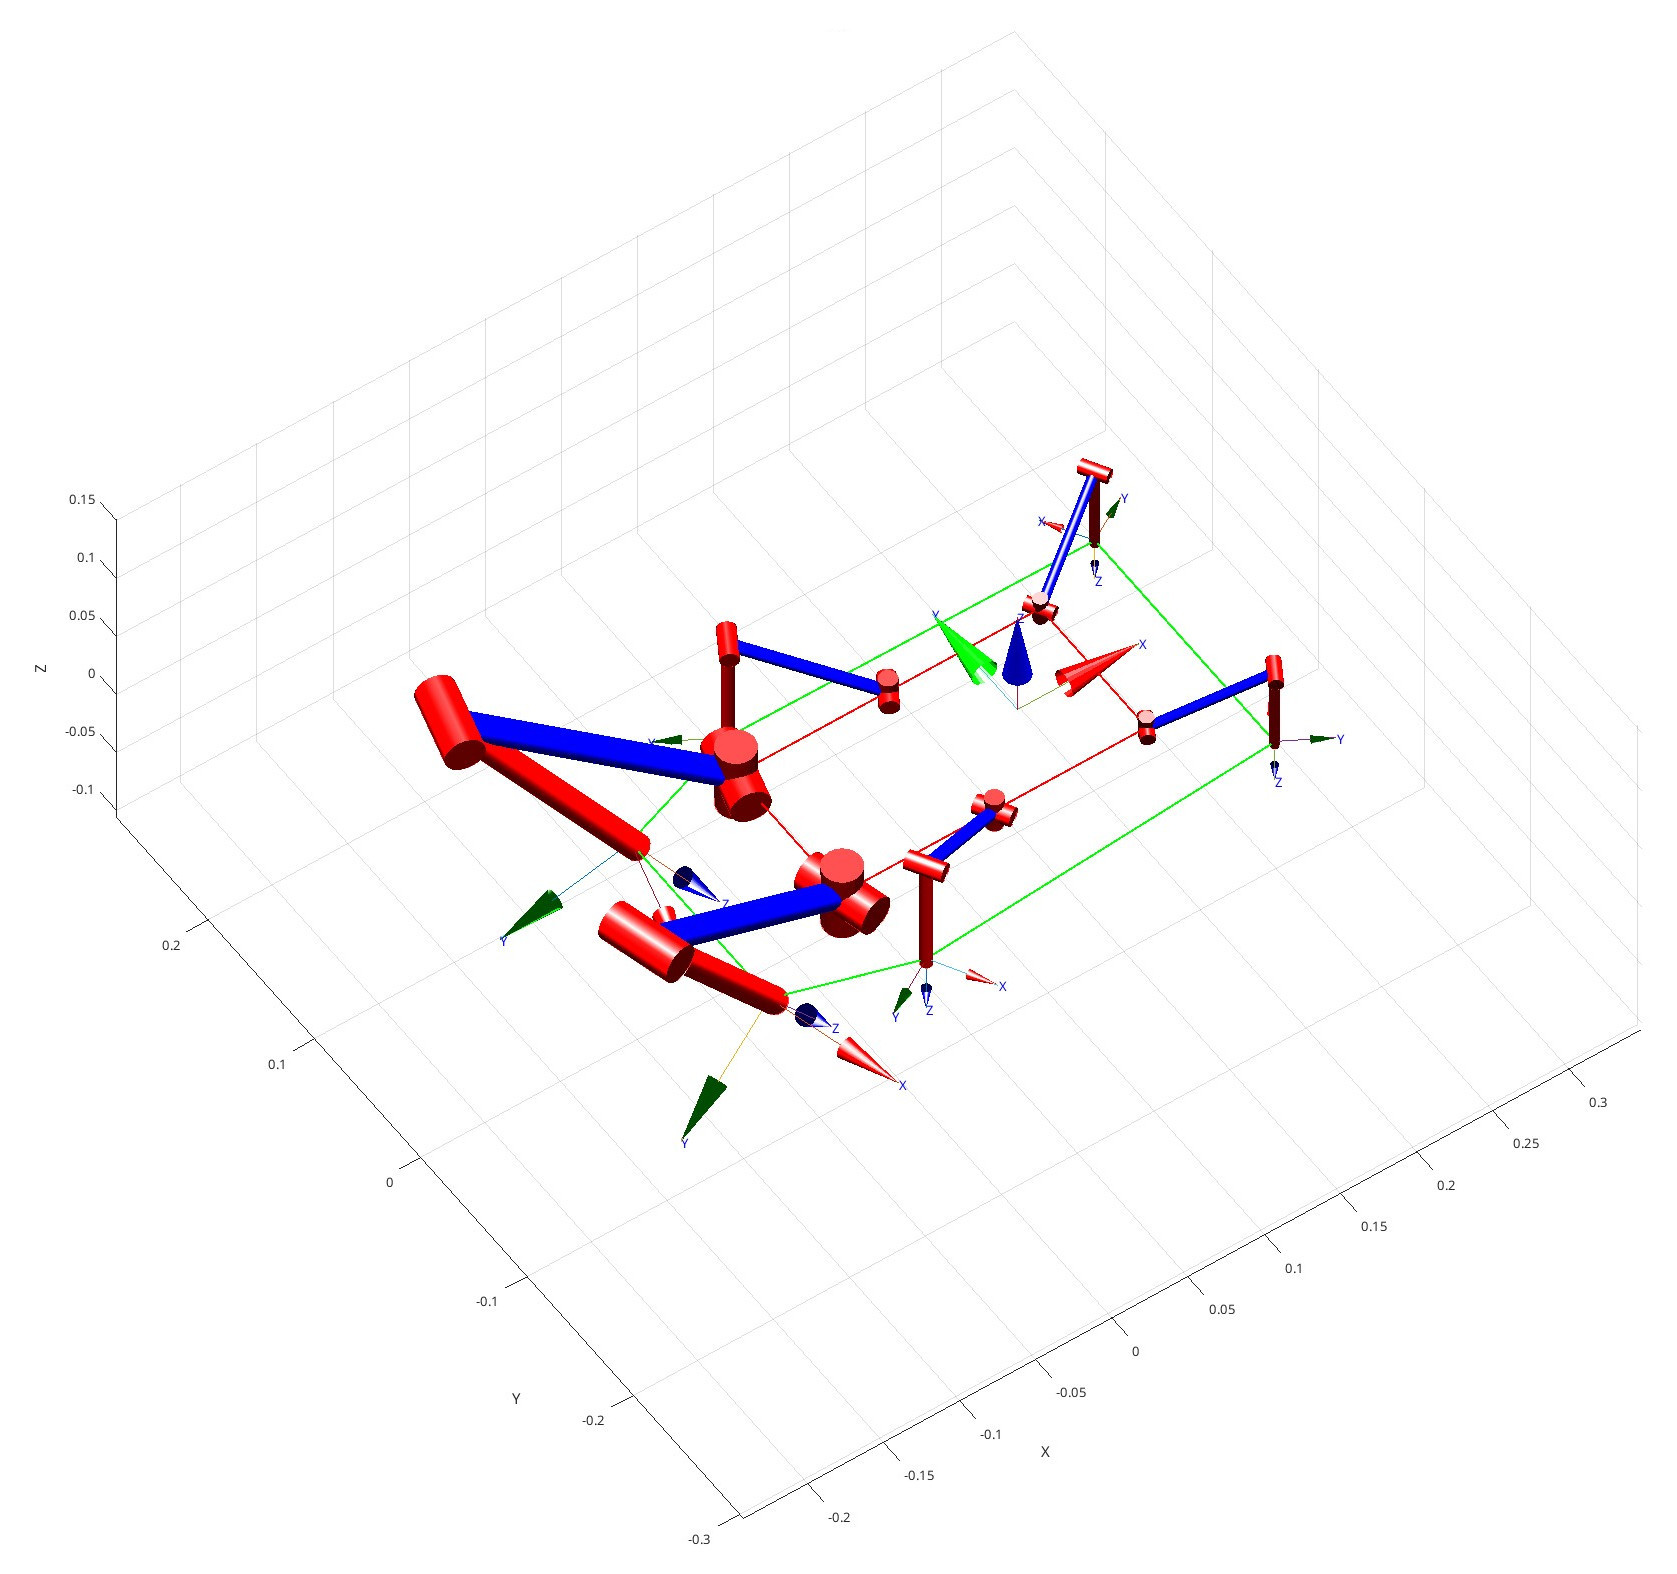
\includegraphics[width=0.5\textwidth]{Images/img_ch3/jumping_config.jpg}}
    \subfloat[ATBVME and legs BVME, orthographic view\label{fig:jumping_ME_ortho}]
    {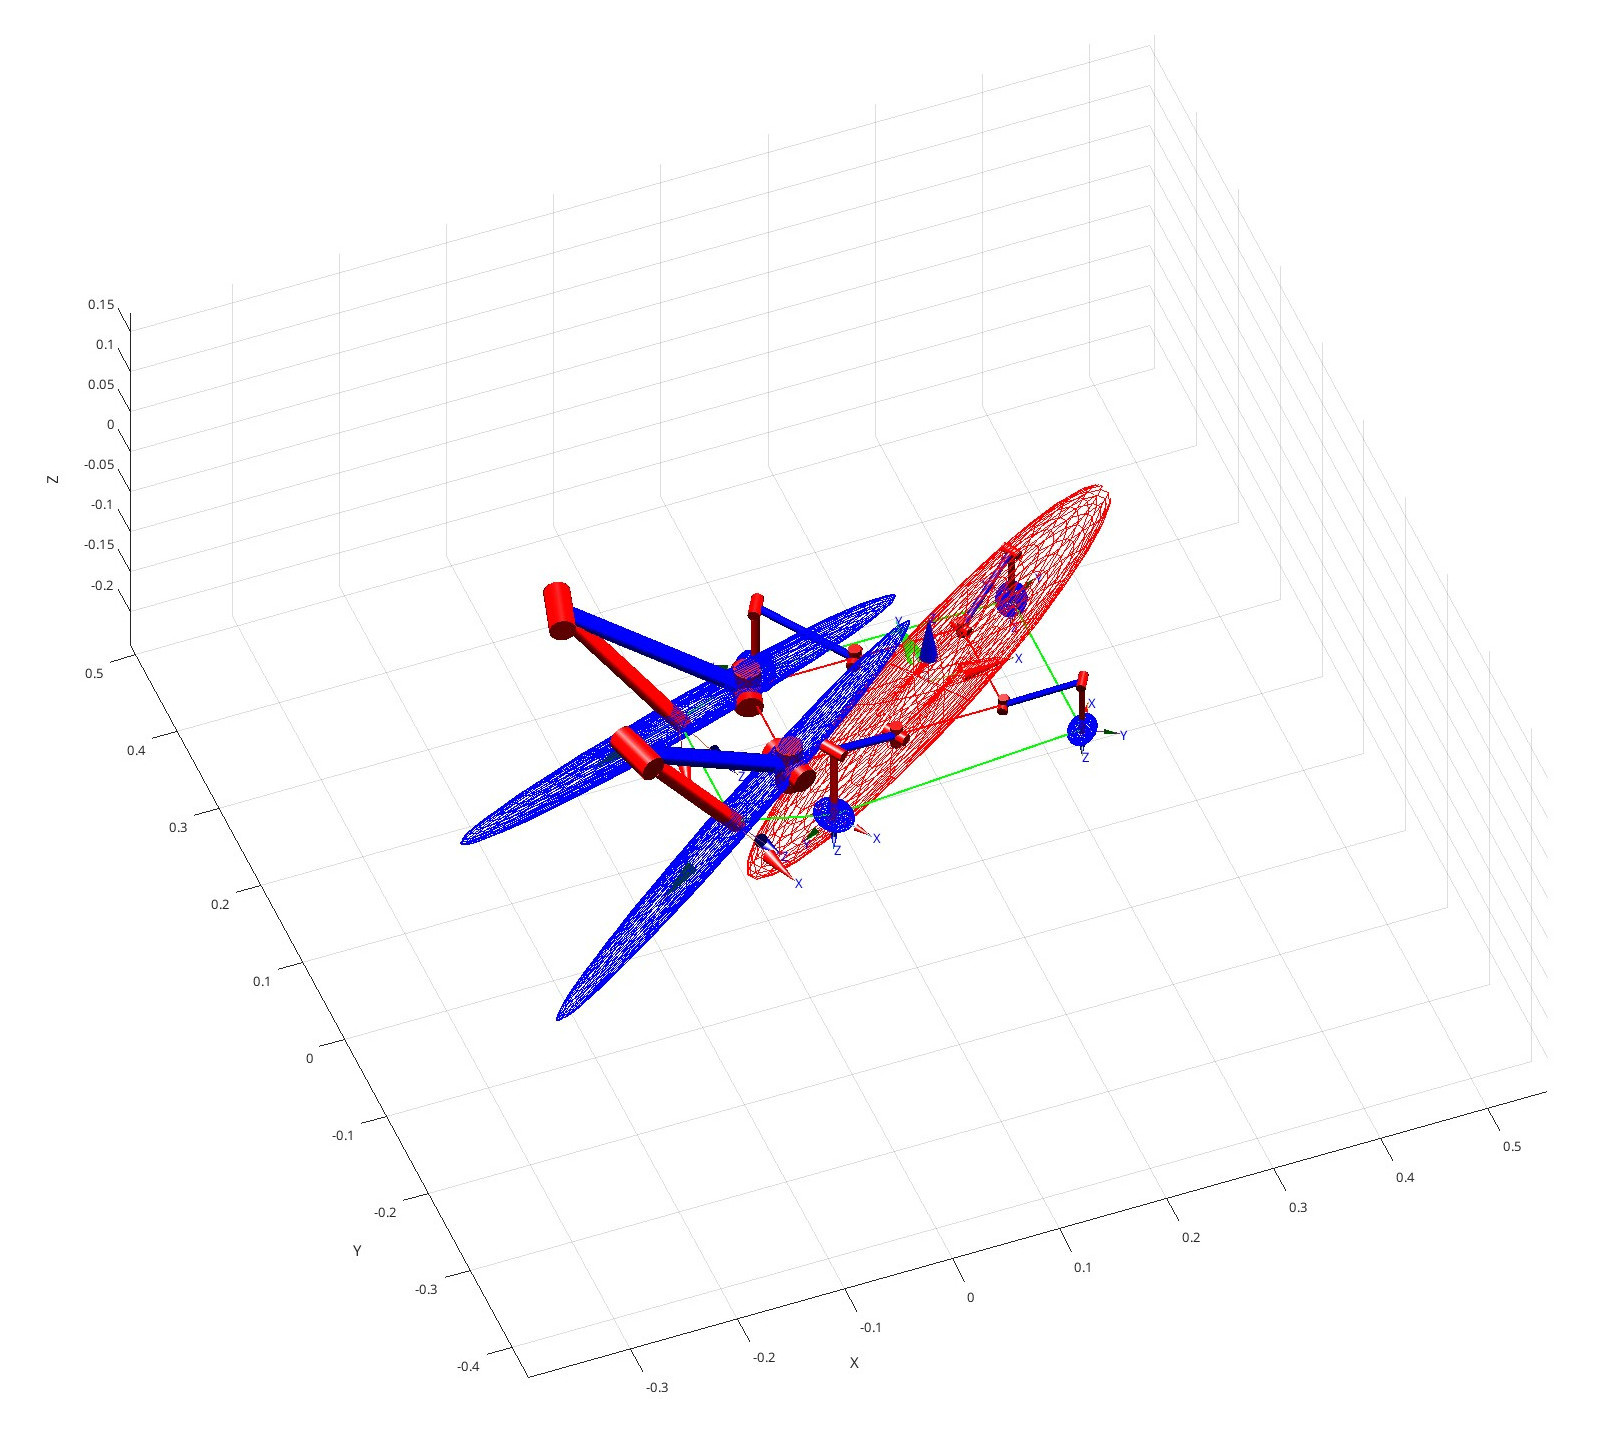
\includegraphics[width=0.5\textwidth]{Images/img_ch3/jumping_ME_ortho.jpg}}\\
    \subfloat[ATBVME and legs BVME, xz view\label{fig:jumping_ME_xz}]
    {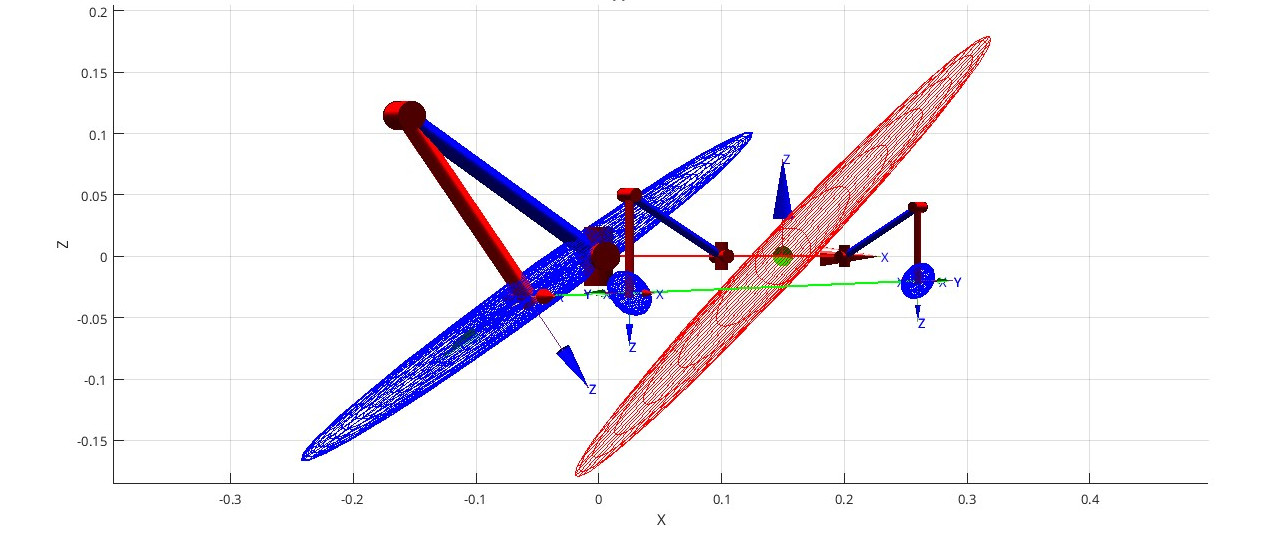
\includegraphics[width=0.6\textwidth]{Images/img_ch3/jumping_ME_xz.jpg}}
    \caption[Manipulability analysis in the jumping configuration]{Manipulability analysis in the jumping configuration}
    \label{fig:grasshopper_model}
\end{figure}


\textbf{2) Jumping Configuration, Sensitivity Analysis}\\
The changes in the ATBVME, when different back leg configurations are considered, are interesting to analyze if the results are consistent with the real biomechanics. 

The jumping configuration of the grasshopper is not only the one in (\ref{eq:jumping_config}), but a set of configurations around the one previously defined, according to the desired jump direction. Releasing the femur-to-tibia (F2T) joint should change the "explosive motion direction". As a limitation of a pure kinematic model, here the spring-like behavior of the extensor muscle is not modeled as a reaction to contraction release, but with the higher speed limit of the F2T joint. For this reason, even when not contracted, back legs give a high-velocity manipulability effect, but configurations far from the jumping one are expected to be disadvantages for this task. 

The results in changing the coxa-to-femur (C2F) and femur-to-tibia (F2T) are reported in Fig.\ref{fig:jumping_changes} in configurations where the back legs touches the ground. Finally, uncommon configurations with wider back legs (B2C angles sensitivity) are reported in Fig.\ref{fig:b2c_changes}, highlighting why these are not common configurations. 


\begin{figure}[H]
    \centering
    \subfloat[$C2F=-30^\circ$, $C2F=160^\circ$, xy view\label{fig:jumping_neg30_160_xy}]{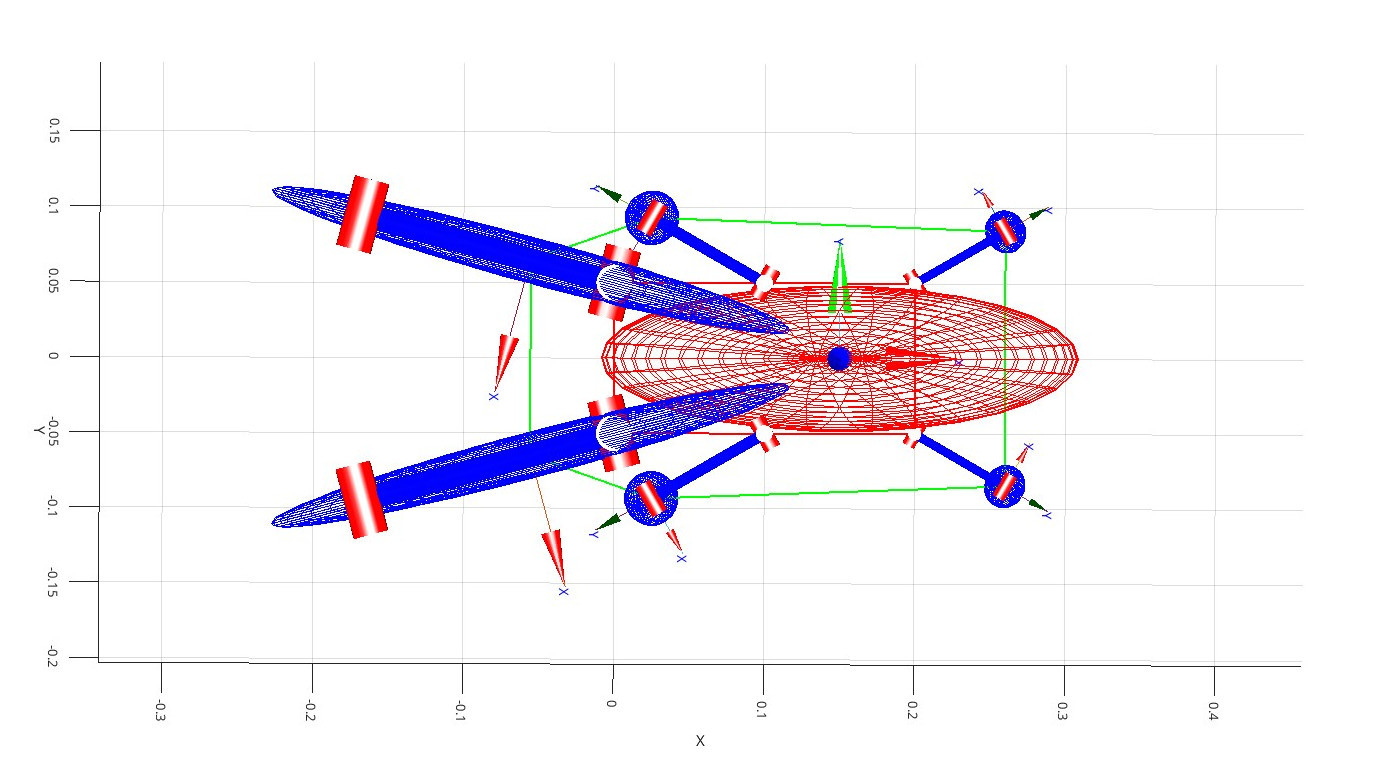
\includegraphics[width=0.50\textwidth]{Images/img_ch3/jumping_neg30_160_xy.jpg}}
    \subfloat[$C2F=-30^\circ$, $C2F=160^\circ$, xz view\label{fig:jumping_neg30_160}]{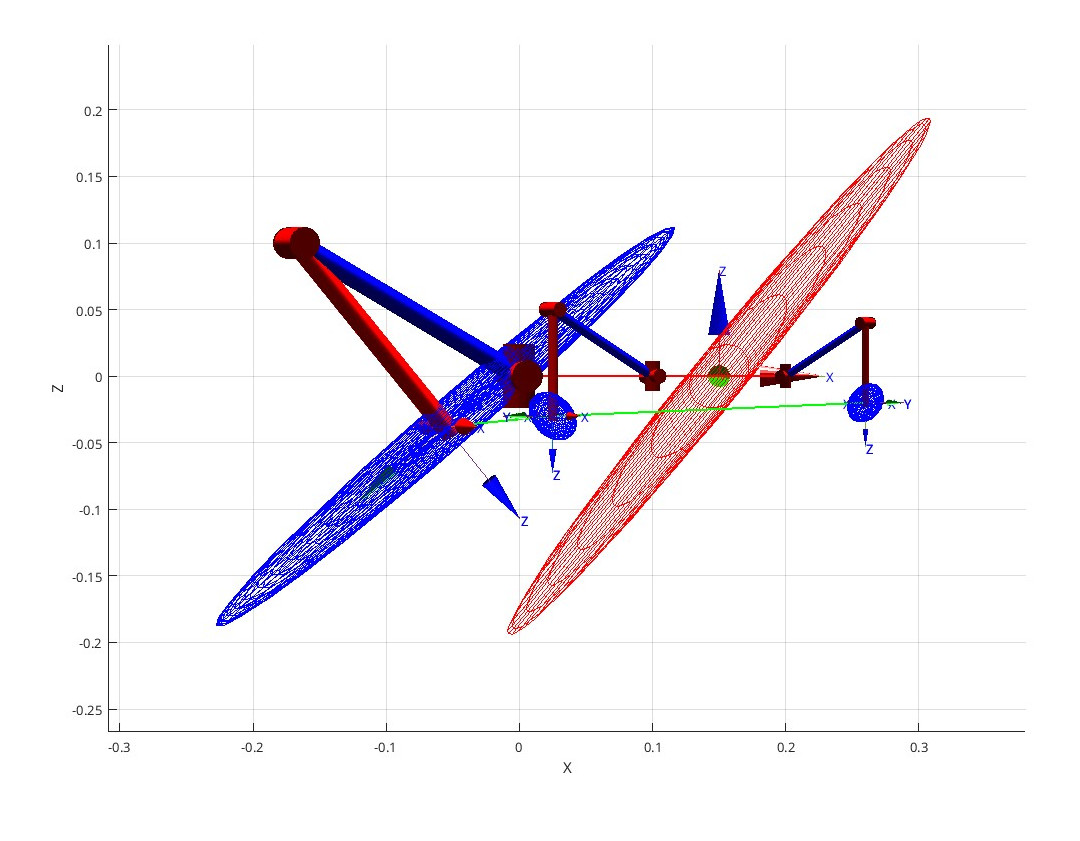
\includegraphics[width=0.45\textwidth]{Images/img_ch3/jumping_neg30_160.jpg}}\\
    \subfloat[$C2F=-20^\circ$, $C2F=170^\circ$, xz view\label{fig:jumping_neg20_170}]
    {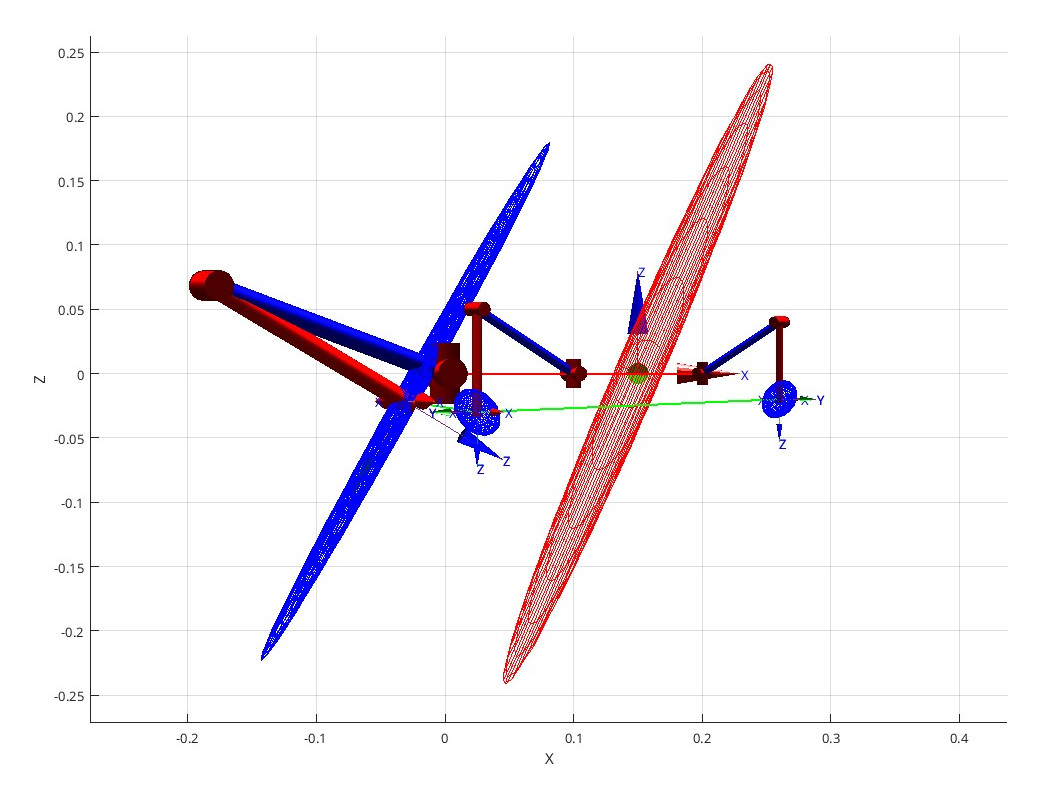
\includegraphics[width=0.45\textwidth]{Images/img_ch3/jumping_neg20_170.jpg}}
    \subfloat[$C2F=-20^\circ$, $C2F=50^\circ$, xz view\label{fig:jumping_neg20_50}]
    {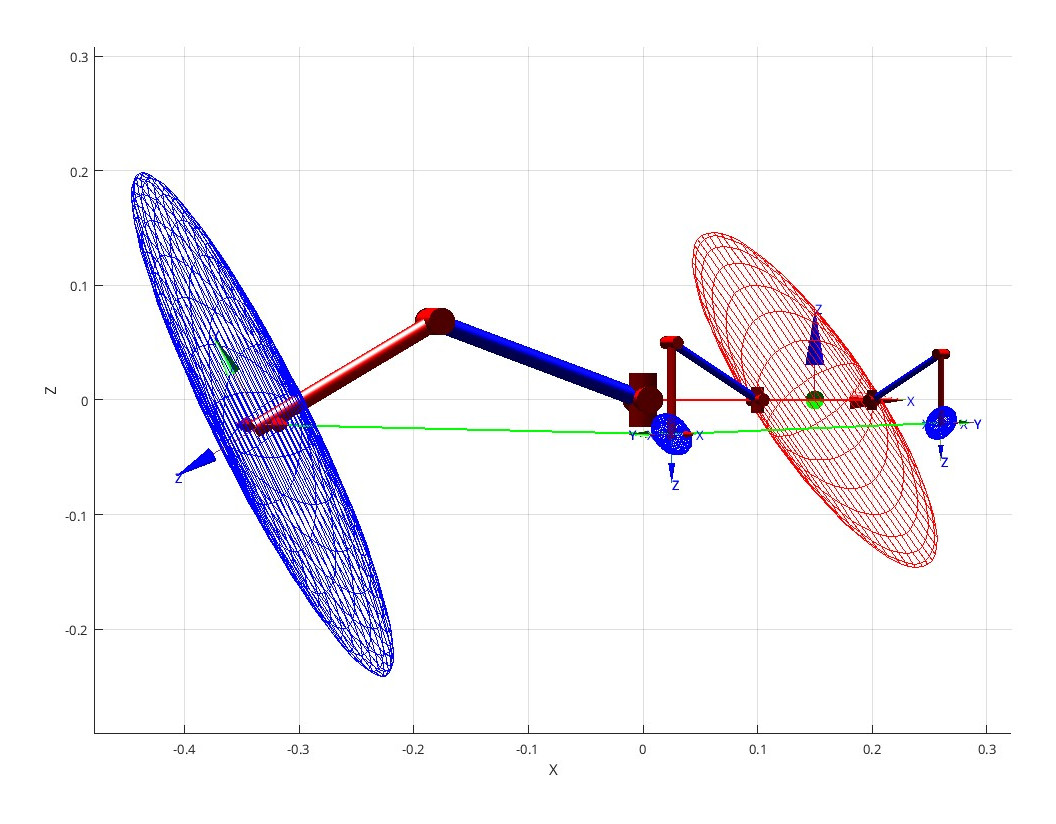
\includegraphics[width=0.45\textwidth]{Images/img_ch3/jumping_neg20_50.jpg}}
    \caption[C2F and F2T jumping sensitivity]{C2F and F2T jumping sensitivity, maintaining $B2C=-15^\circ$.}
    \label{fig:jumping_changes}
\end{figure}

In all the configurations tested and reported above in Fig.\ref{fig:jumping_changes}, the ellipsoid is oriented in the x-axis direction, but the major axis highly depends on the back legs configuration. 
Different legs' interactions with the ground (here modeled just kinematically by the configurations) affect the jump performances and the direction. 

Intuitively, if the back legs are wider, jumping capability gets distributed in a wider range of directions, using efficiency, and the BME is coherent with this, as reported in Fig.\ref{fig:b2c_changes}.

In conclusion, an asymmetric configuration of the back legs is reported in Fig.\ref{fig:asymmetry}, resulting in consistent ellipsoids with the expected unnatural jumping capability.

\begin{figure}[H]
    \centering
    \subfloat[$|B2C|=15^\circ$\label{fig:jumping_b2c_neg15}]{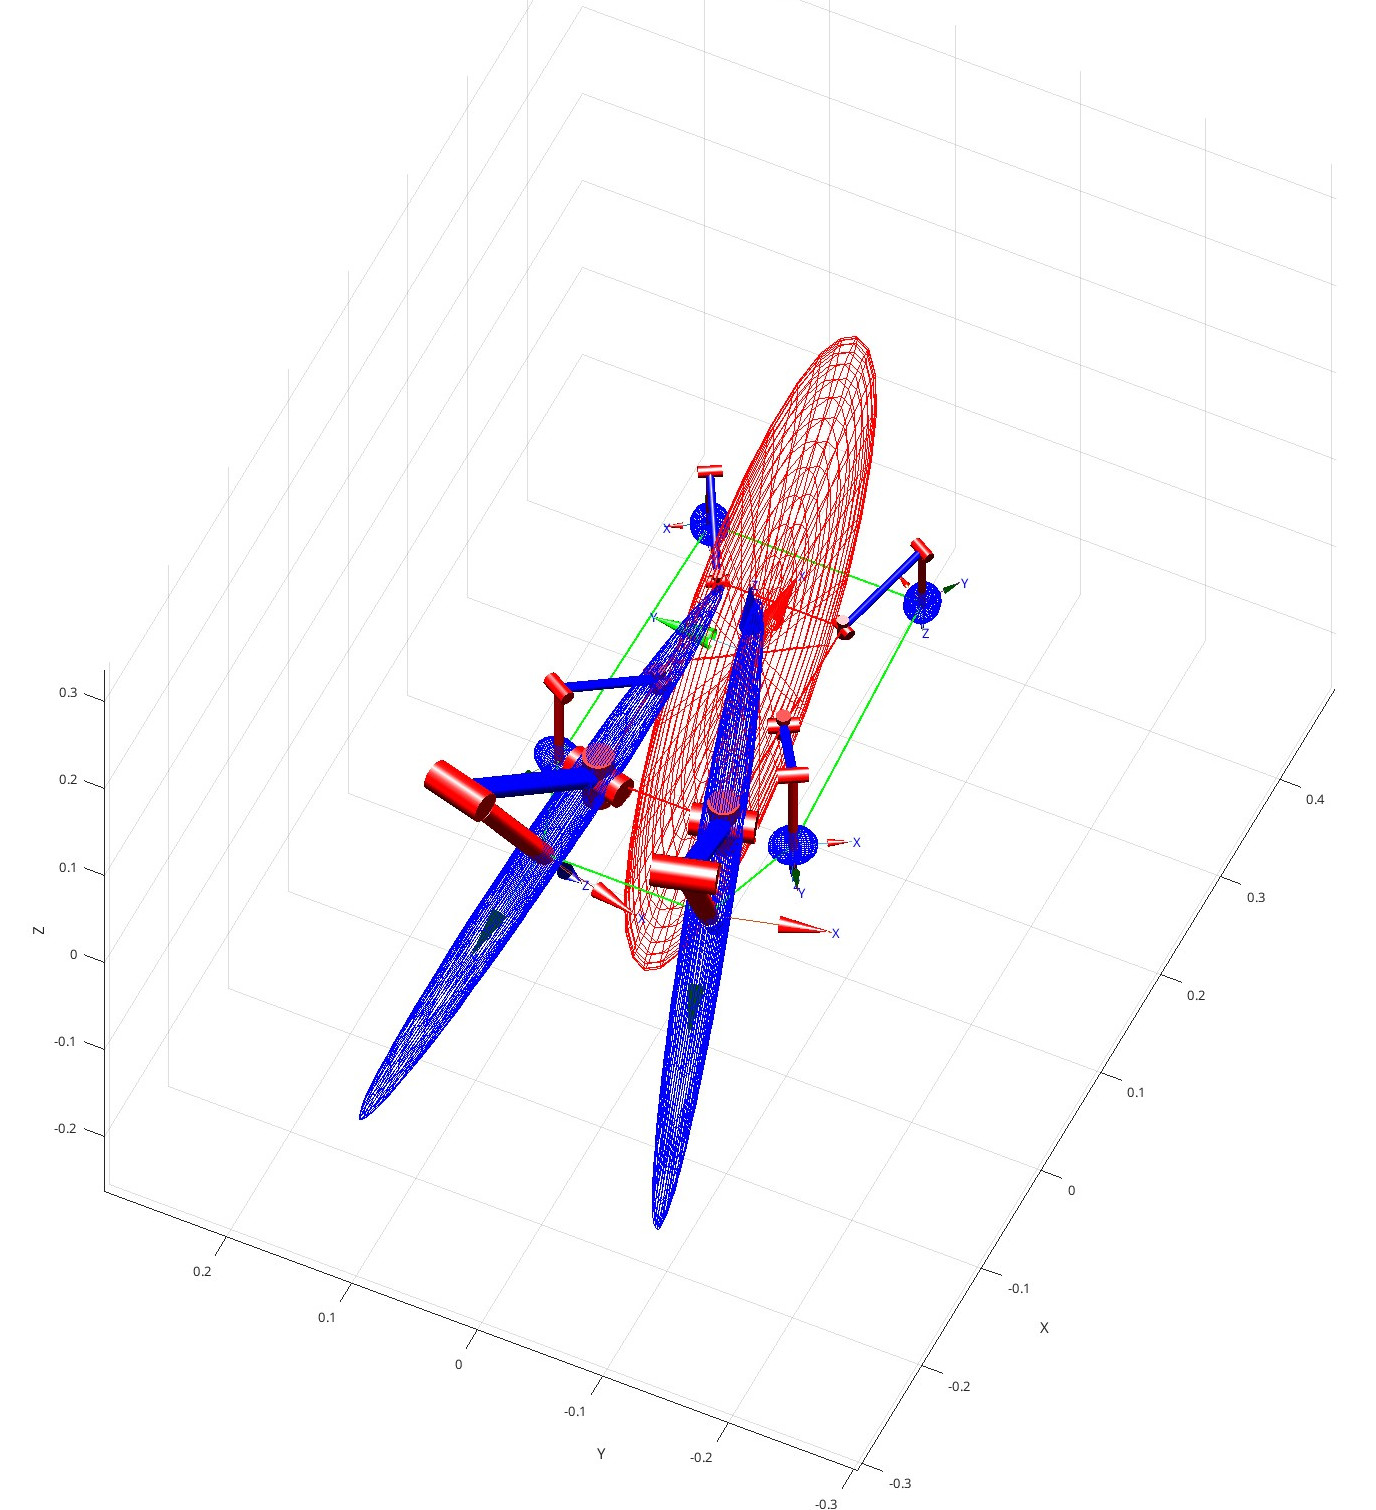
\includegraphics[width=0.4\textwidth]{Images/img_ch3/jumping_b2c_neg15.jpg}}
    \subfloat[$|B2C|=25^\circ$\label{fig:jumping_b2c_neg25}]
    {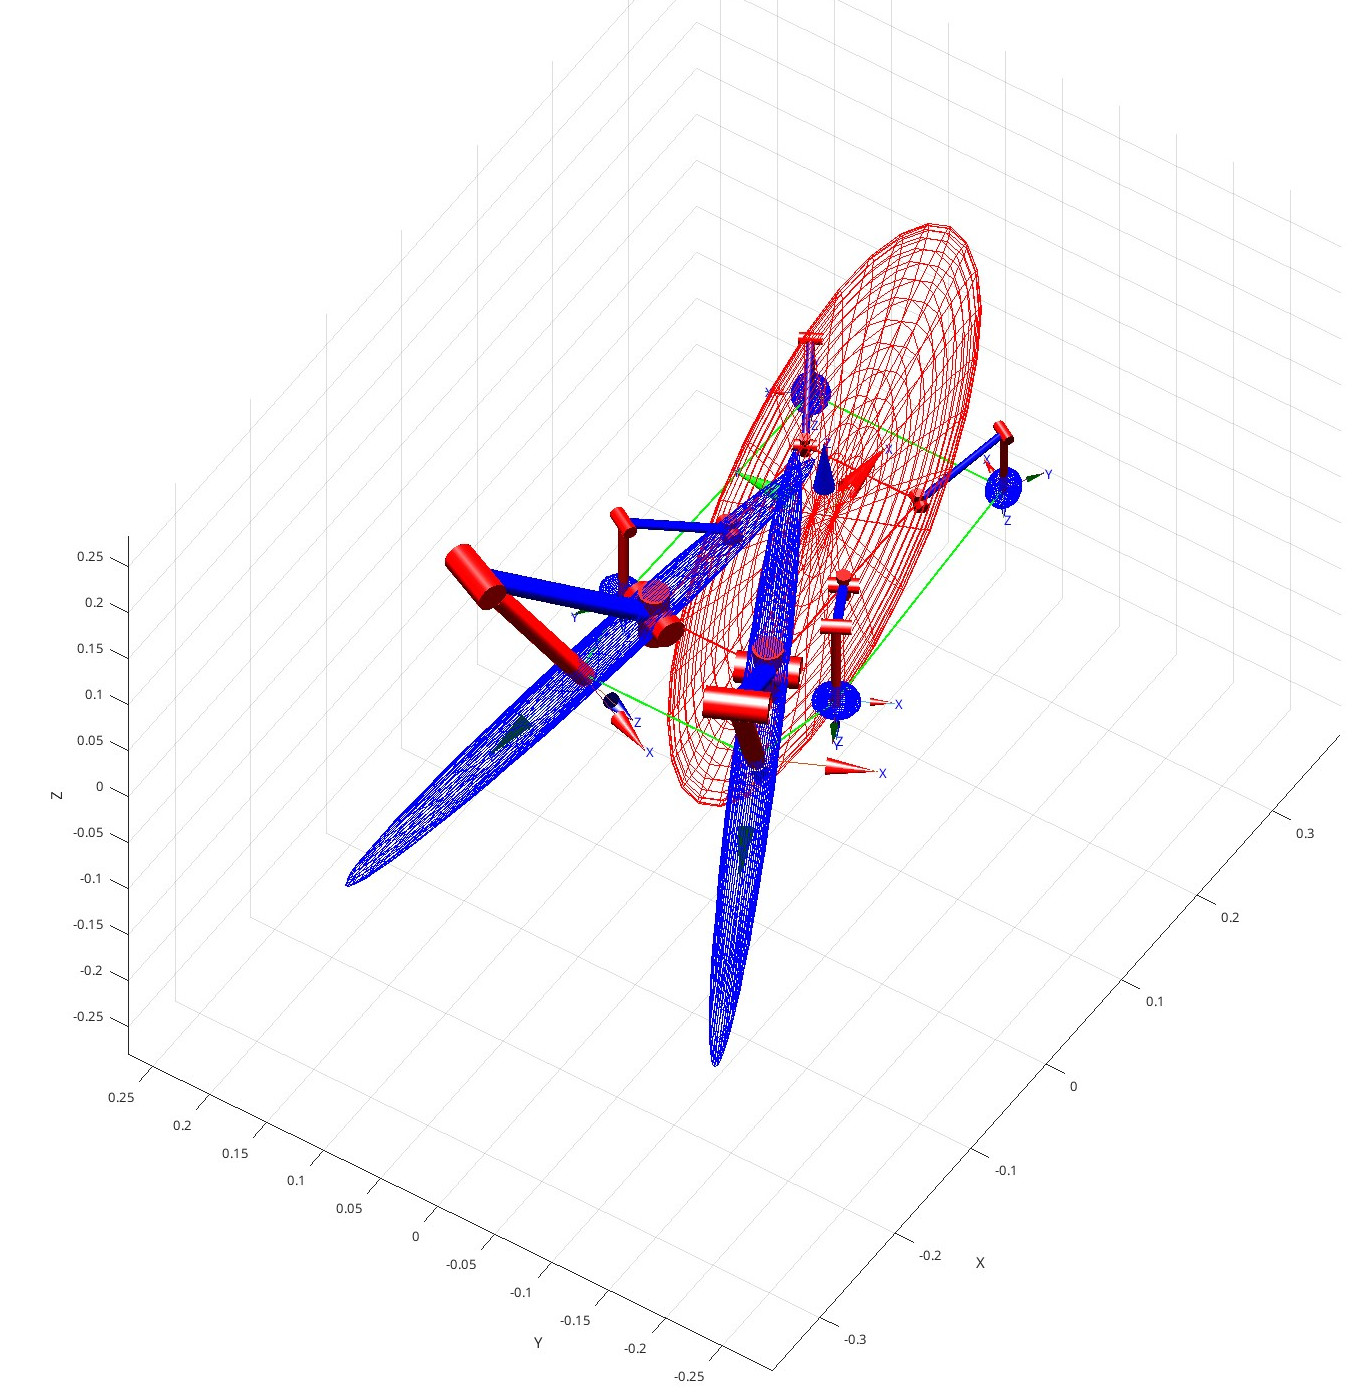
\includegraphics[width=0.4\textwidth]{Images/img_ch3/jumping_b2c_neg25.jpg}}\\
    \subfloat[$|B2C|=45^\circ$\label{fig:jumping_b2c_neg45}]
    {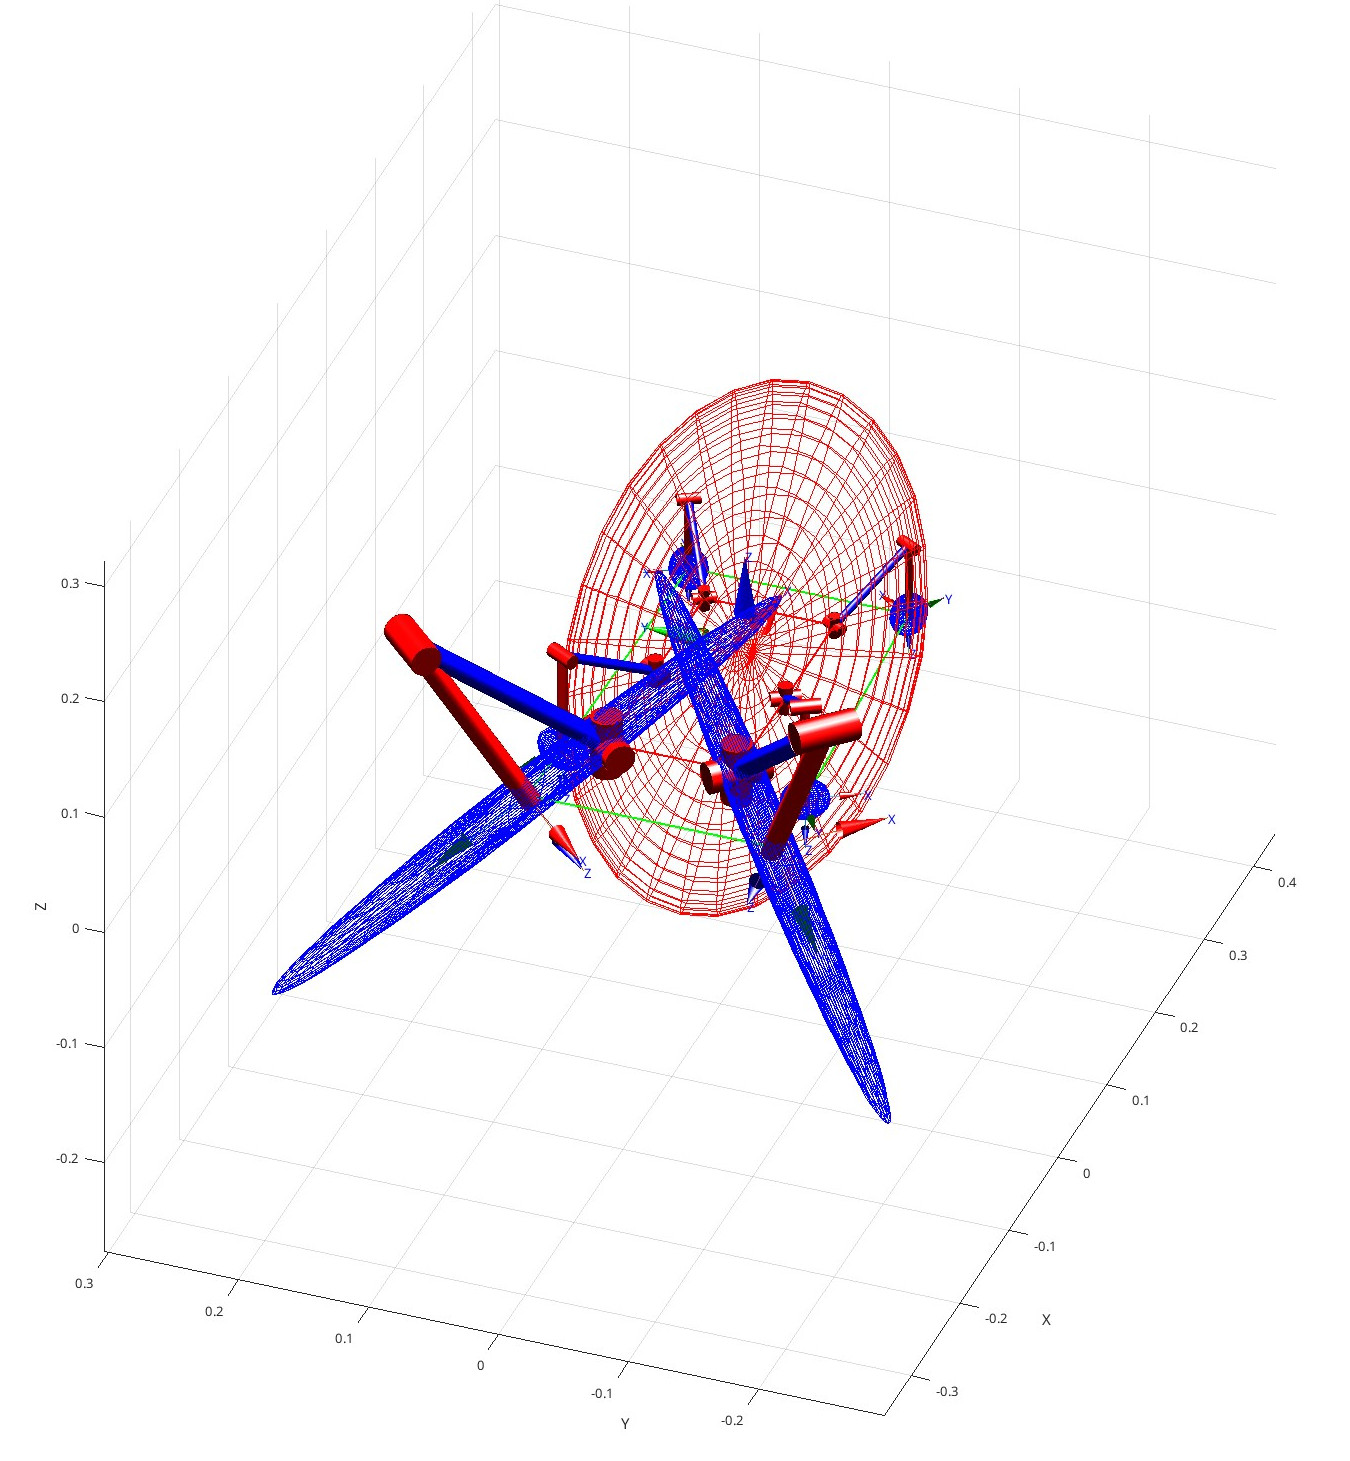
\includegraphics[width=0.4\textwidth]{Images/img_ch3/jumping_b2c_neg45.jpg}}
    \subfloat[$|B2C|=70^\circ$\label{fig:jumping_b2c_neg70}]
    {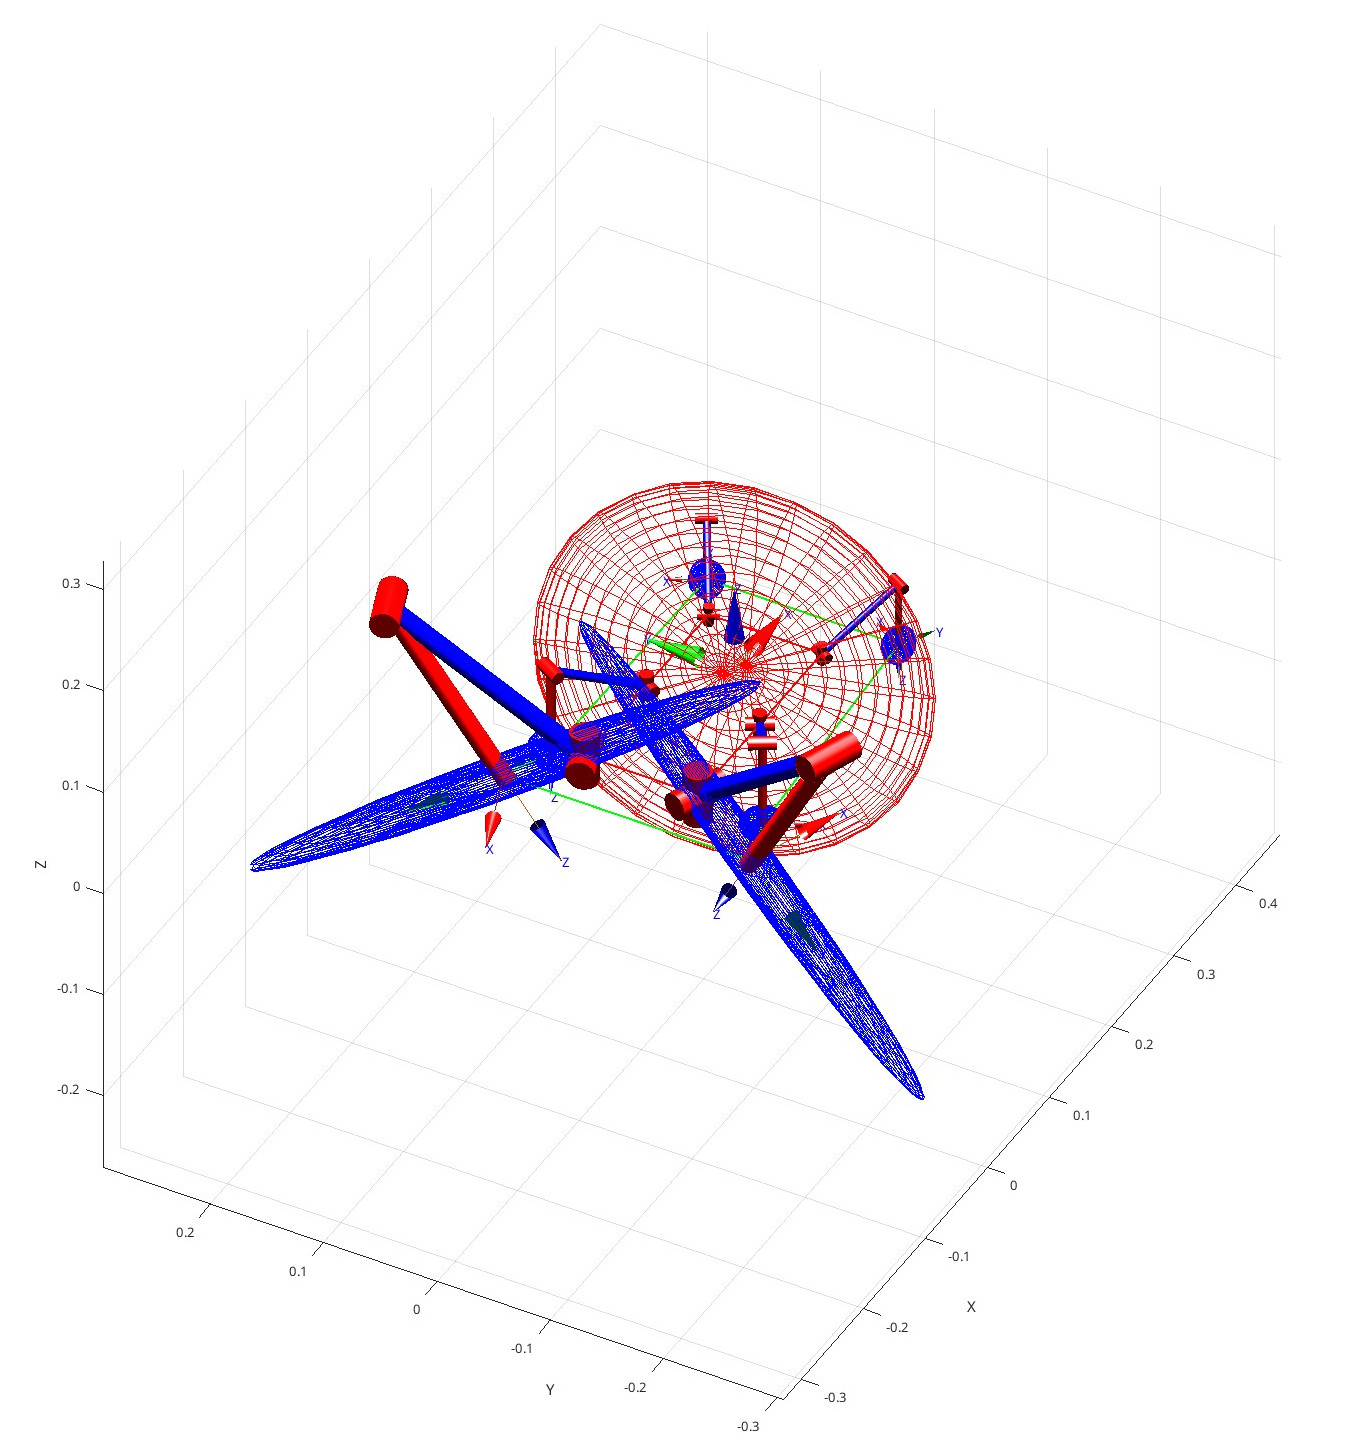
\includegraphics[width=0.4\textwidth]{Images/img_ch3/jumping_b2c_neg70.jpg}}\\
    \subfloat[$|B2C|=15^\circ$, yz view\label{fig:jumping_b2c_neg15_yz}]
    {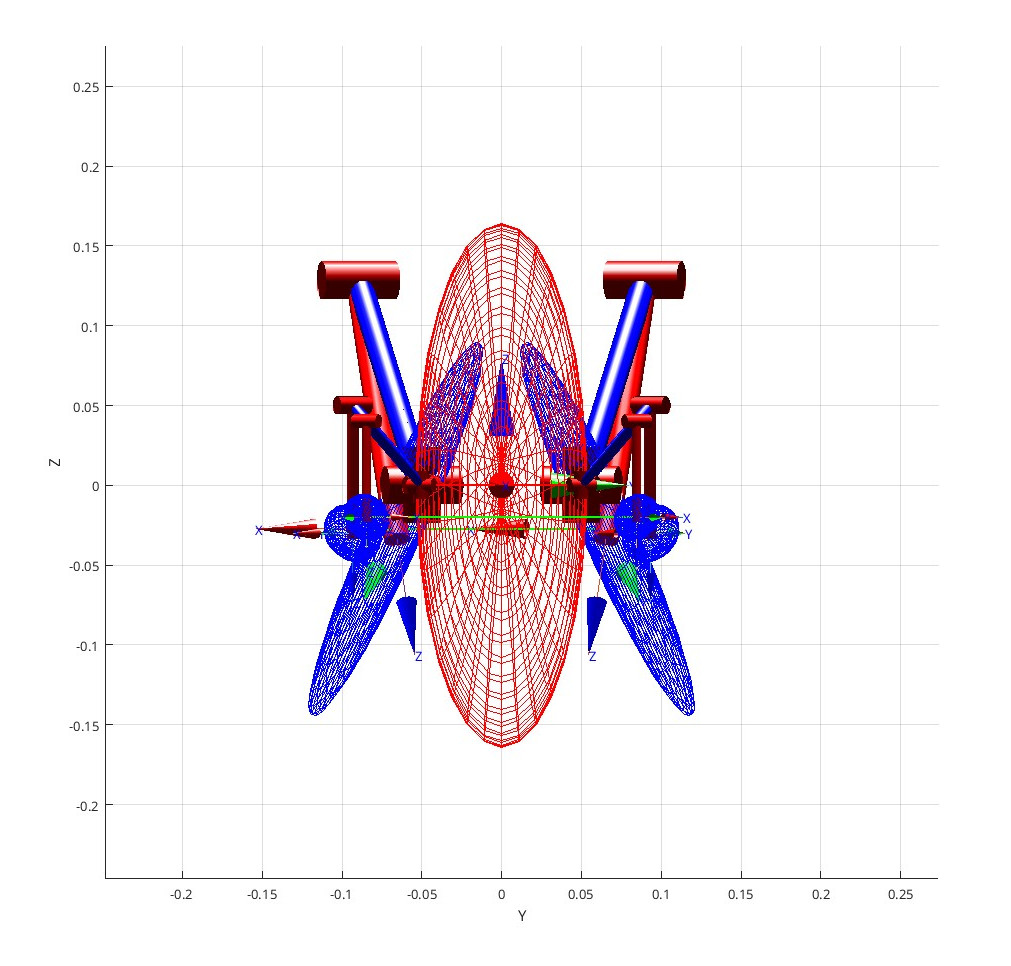
\includegraphics[width=0.4\textwidth]{Images/img_ch3/jumping_b2c_neg15_yz.jpg}}
    \subfloat[$|B2C|=70^\circ$, yz view\label{fig:jumping_b2c_neg70_yz}]
    {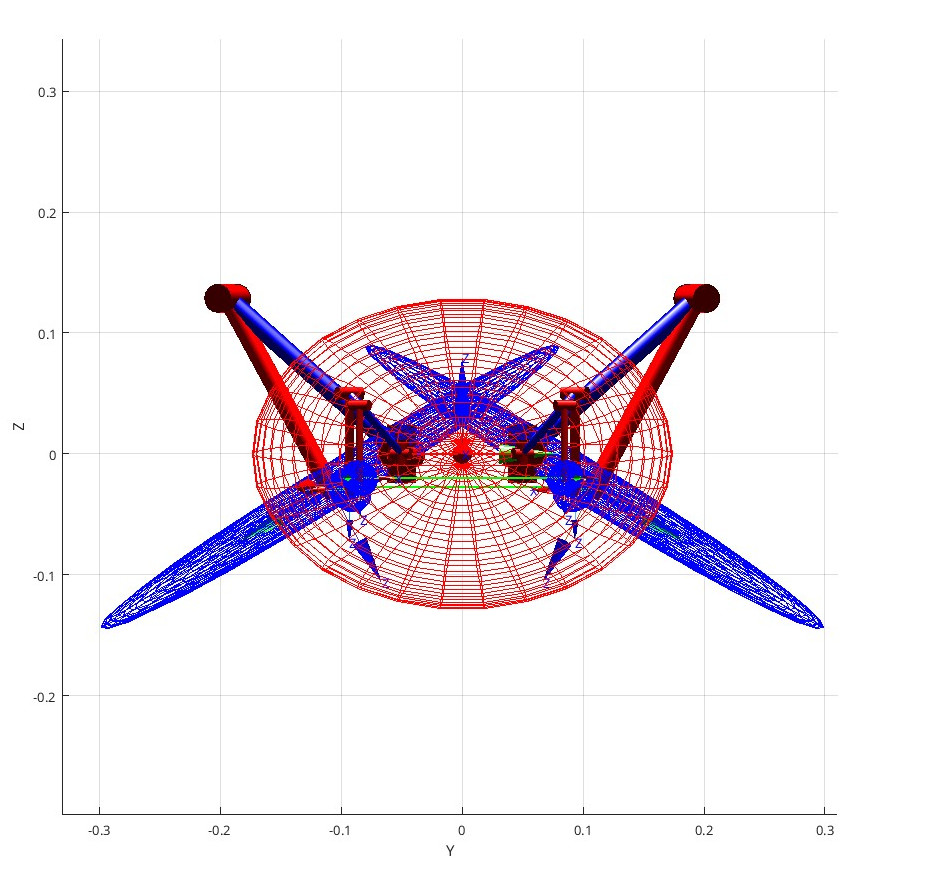
\includegraphics[width=0.4\textwidth]{Images/img_ch3/jumping_b2c_neg70_yz.jpg}}
    \caption[B2C jumping sensitivity]{B2C jumping sensitivity, maintaining $C2F=-40^\circ$ and $F2T=160^\circ$}
    \label{fig:b2c_changes}
\end{figure}

\begin{figure}[H]
    \centering
    \subfloat[$L_{F2T}=120^\circ$ $R_{F2T}=160^\circ$\label{fig:jumping_Lf2t_120_Rf2t_160}]{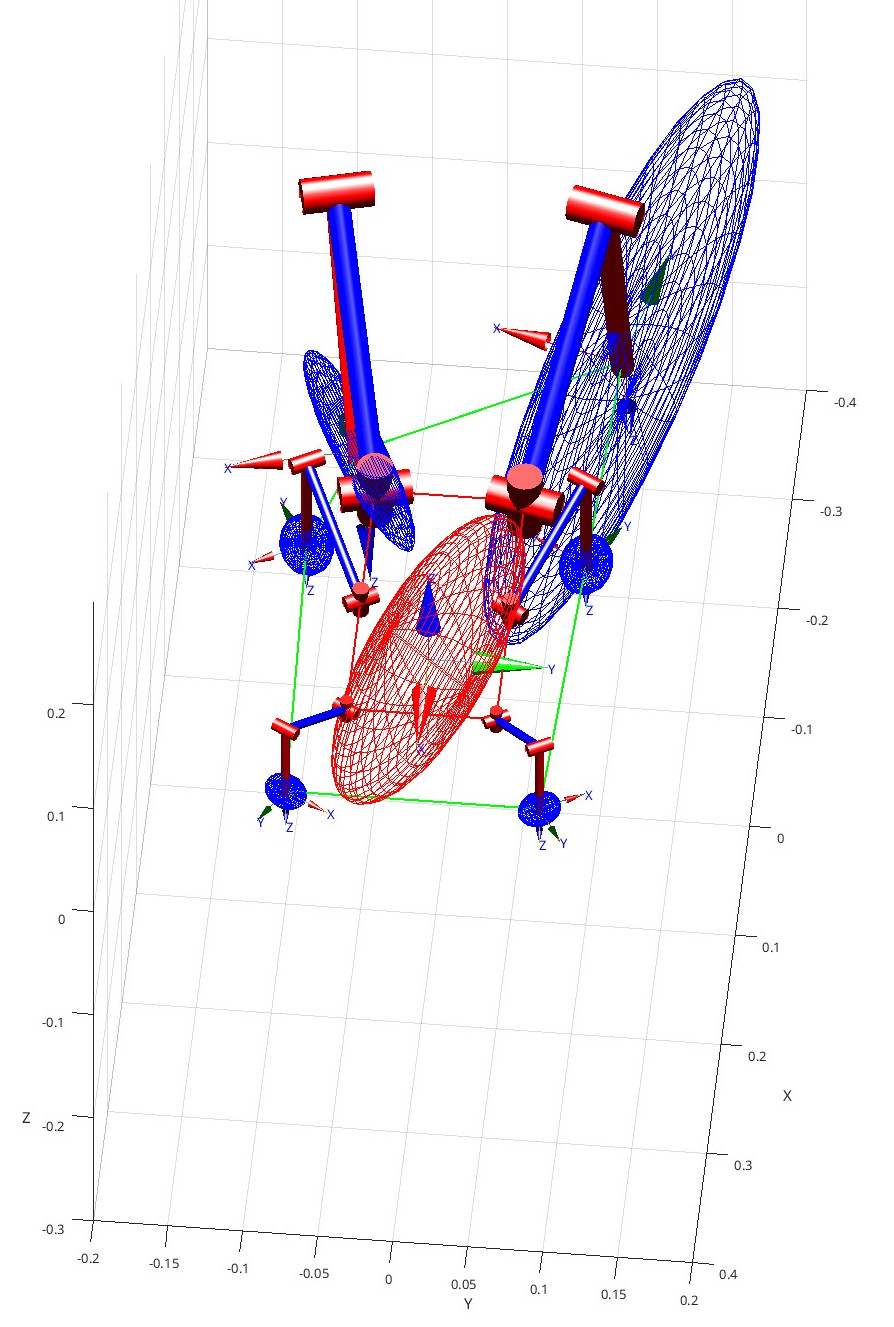
\includegraphics[width=0.35\textwidth]{Images/img_ch3/jumping_Lf2t_120_Rf2t_160.jpg}}
    \subfloat[$L_{F2T}=120^\circ$ $R_{F2T}=160^\circ$, yz view\label{fig:jumping_Lf2t_120_Rf2t_160_yz}]
    {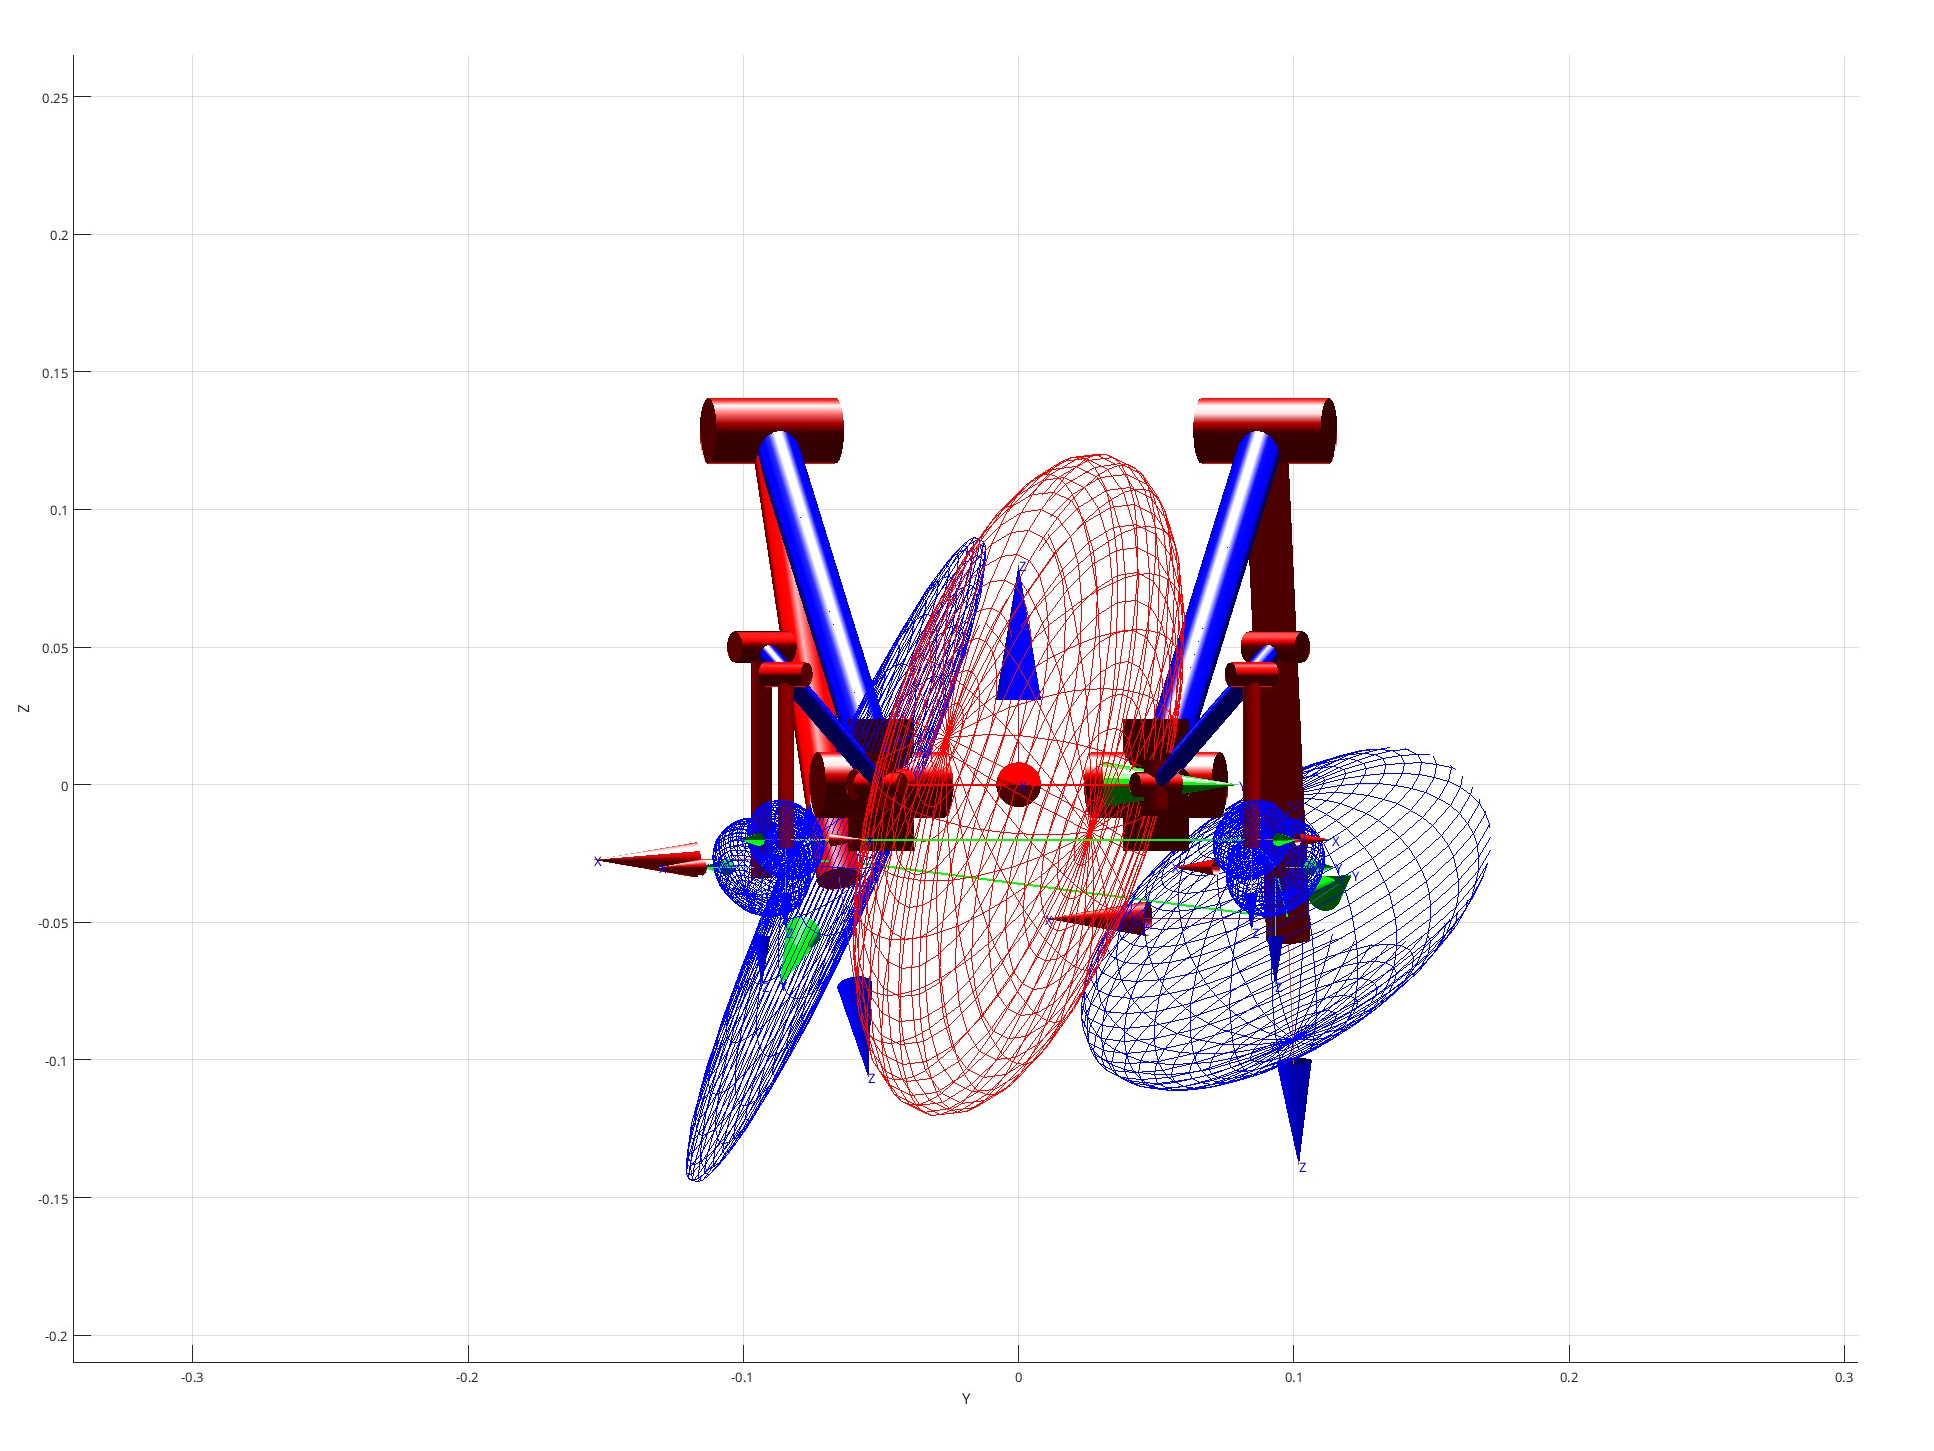
\includegraphics[width=0.5\textwidth]{Images/img_ch3/jumping_Lf2t_120_Rf2t_160_yz.jpg}}\\
    \caption[Asymmetric back legs performances]{Asymmetric back legs performances, with $|B2C| = -15^{\circ}$ and $C2F = -40^{\circ}$.}
    \label{fig:asymmetry}
\end{figure}

\textbf{3) Failure of one back leg}\\
Analyzing possible points of failure is interesting, in this case, to see if the behaviors described by the ellipsoid are coherent. For a robotic system instead, it can provide useful information to define recovery behaviors.  

In the results here, the jumping leg is considered in the configuration:\\ 
$\textbf{q}_{jump,B} = \begin{bmatrix}
    -15^\circ & -40^\circ & 160^\circ
\end{bmatrix}^T$ \\While the other one is irrelevant, since not involved in the motion of the base (removing the ground interaction, represented by the fact that its ellipsoid is green).   

The clear change of maximum direction of the ATBVME in Fig.\ref{fig:one_fail} is coherent with the expected loss of one-leg jumping mobility. 

\begin{figure}[H]
    \centering
    \subfloat[Manipulability without back left leg, top view\label{fig:jumping_NO_BL_xy}]{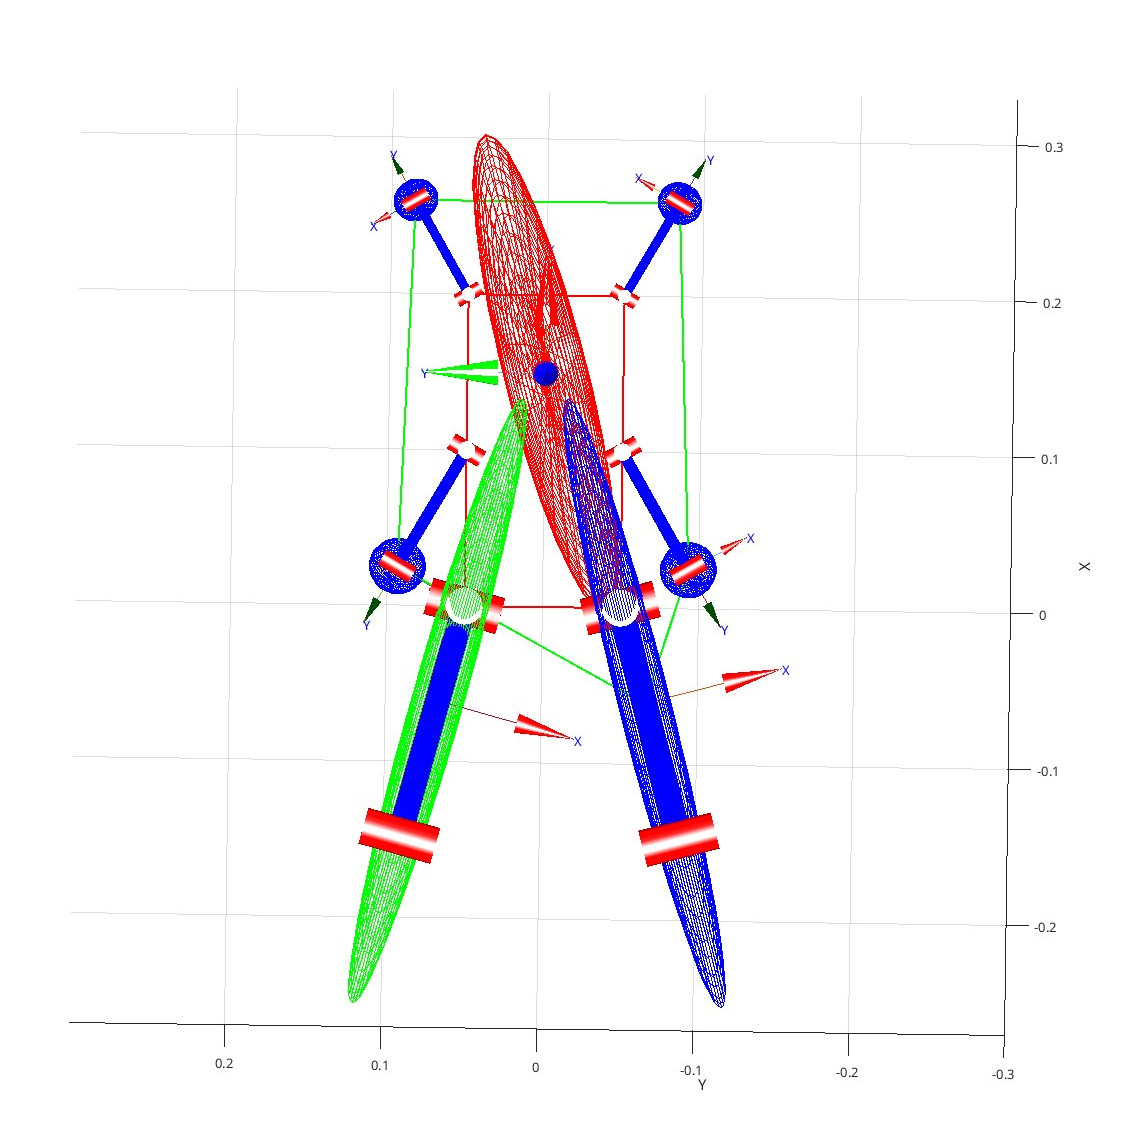
\includegraphics[width=0.5\textwidth]{Images/img_ch3/jumping_NO_BL_xy.jpg}}
    \subfloat[Manipulability without back right leg, top view\label{fig:jumping_NO_BR_xy}]
    {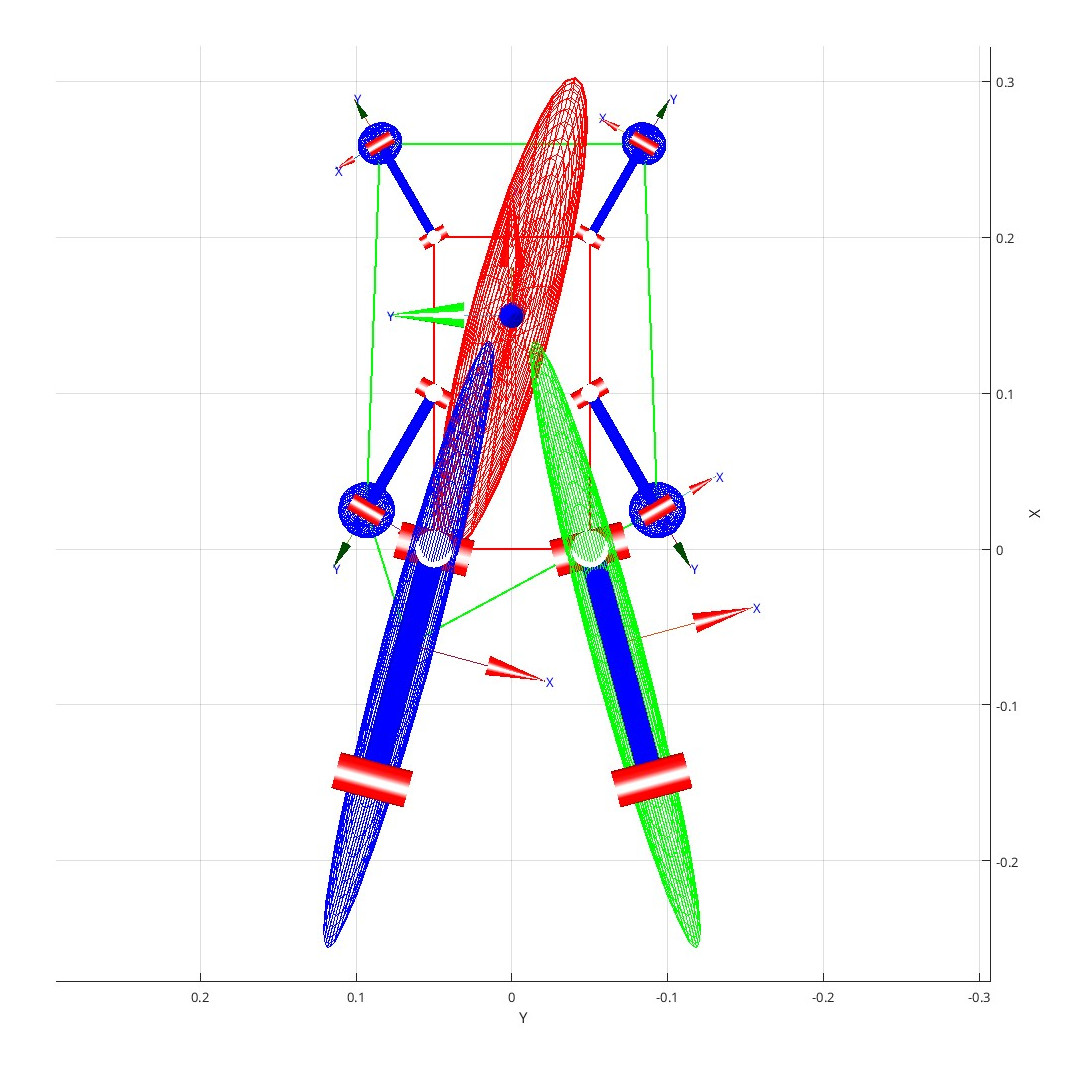
\includegraphics[width=0.5\textwidth]{Images/img_ch3/jumping_NO_BR_xy.jpg}}\\
    \subfloat[Manipulability without back left leg, xz view\label{fig:jumping_NO_BL_xz}]{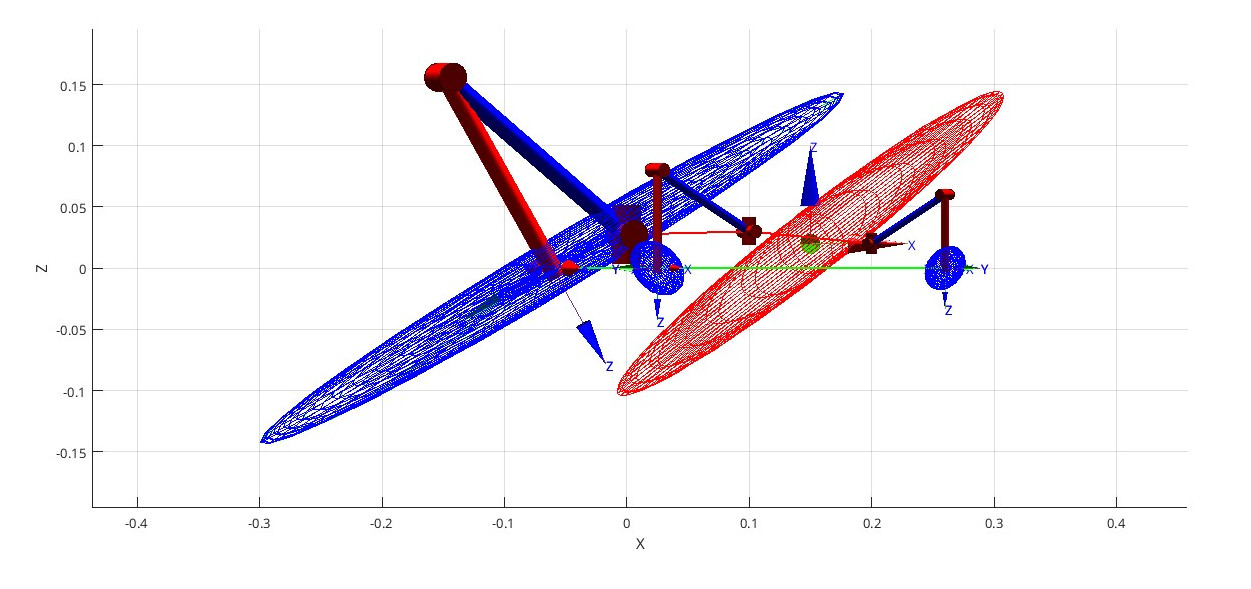
\includegraphics[width=0.5\textwidth]{Images/img_ch3/jumping_NO_BL_xz.jpg}}
    \subfloat[Manipulability without back right leg, xz view\label{fig:jumping_NO_BR_xz}]
    {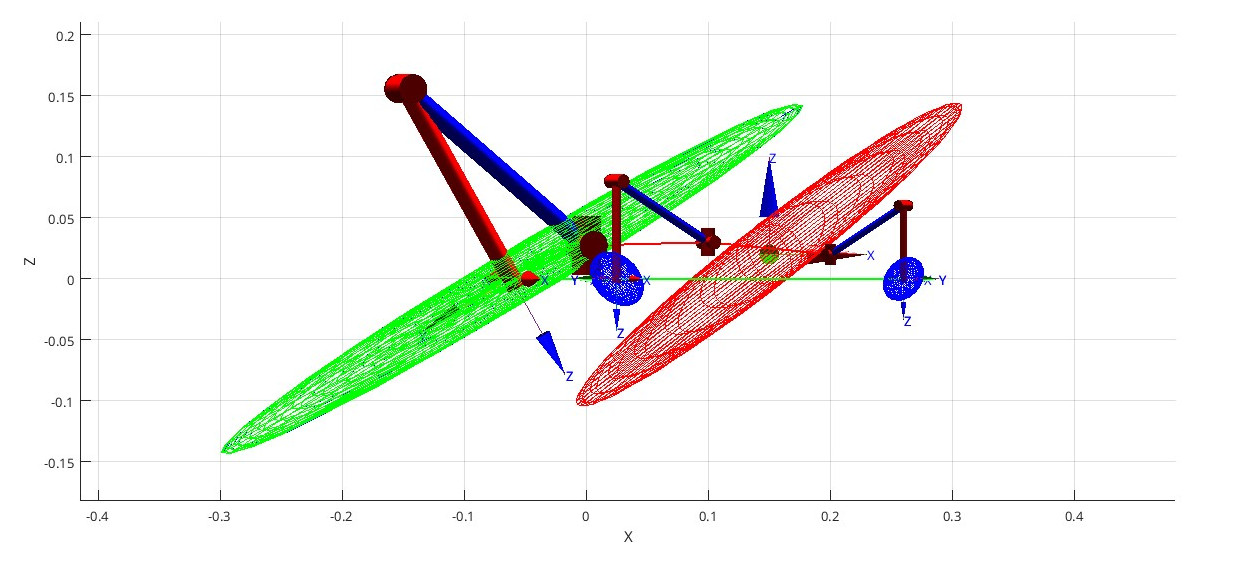
\includegraphics[width=0.5\textwidth]{Images/img_ch3/jumping_NO_BR_xz.jpg}}
    \caption[Jumping performances without one of the back leg]{Jumping performances without one of the back leg.}
    \label{fig:one_fail}
\end{figure}

\textbf{4) Failure of both back legs}\\
Considering a critical failure, in principle it is expected a complete loss of the jumping ability, with only a limited motion capability given by the weak front legs.
The results are reported in Fig.\ref{fig:both_leg_fail}, with a small isotropic ellipsoid, without any dominating jumping axis. 

\begin{figure}[H]
    \centering
    \subfloat[Manipulability without jumping legs, xy view\label{fig:jumping_NO_B_xy}]{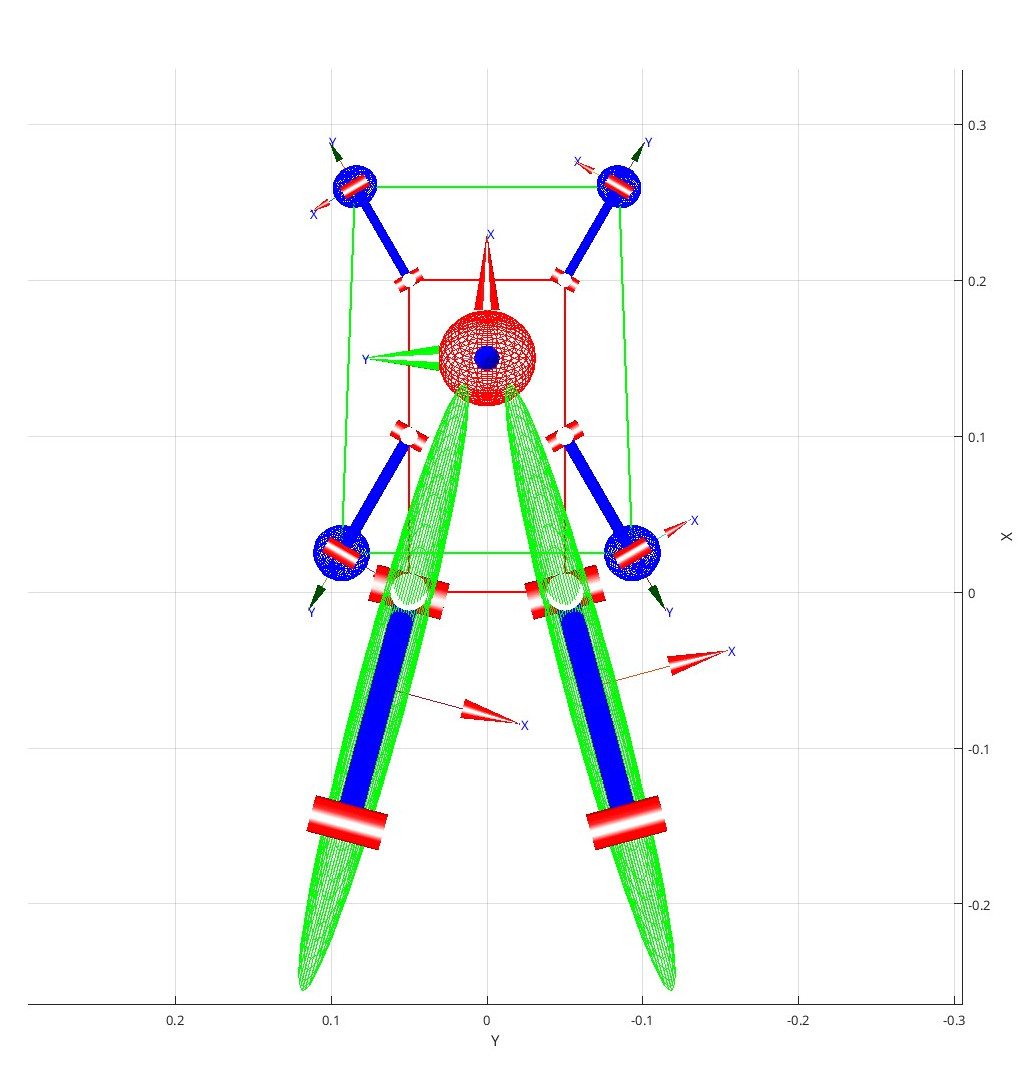
\includegraphics[width=0.5\textwidth]{Images/img_ch3/jumping_NO_B_xy.jpg}}
    \subfloat[Manipulability without jumping legs, xz view\label{fig:jumping_NO_B_xz}]
    {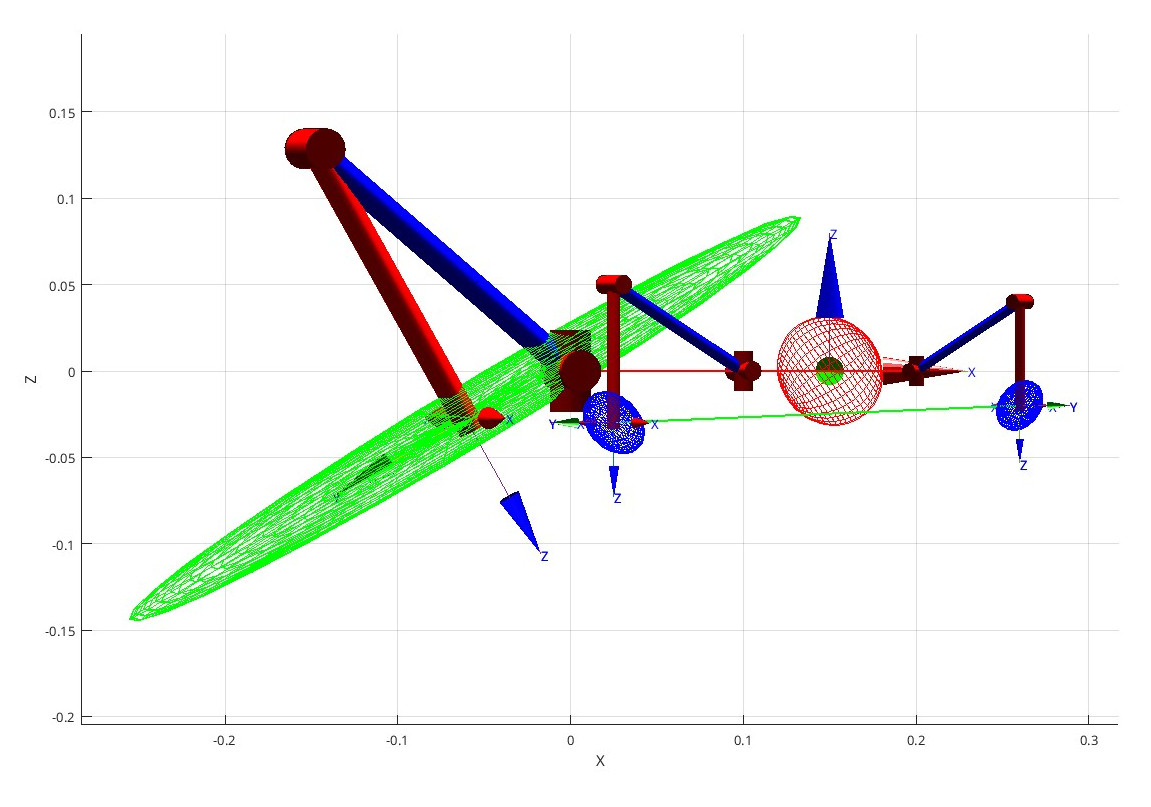
\includegraphics[width=0.5\textwidth]{Images/img_ch3/jumping_NO_B_xz.jpg}}
    \caption[Manipulability without jumping legs]{Manipulability without jumping legs}
    \label{fig:both_leg_fail}
\end{figure}

\textbf{5) CoM position, Sensitivity Analysis}\\
What happens to the manipulability ellipsoid when the CoM position changes is an interesting question. 
This is especially relevant for systems that can 
lose/gain parts or change its structure depending on the task.
Again the back legs are considered in 
$\mathbf{q}_{LB} =\mathbf{q}_{RB} = \begin{bmatrix}
    -15^\circ & -40^\circ & 160^\circ
\end{bmatrix}^T$\\
As reported in Fig.\ref{fig:CoM_changes}, the CoM is translated in the midpoint between the two back legs.
\begin{figure}[H]
    \centering
    \subfloat[xy view\label{fig:jumping_CoM_0_xy}]
    {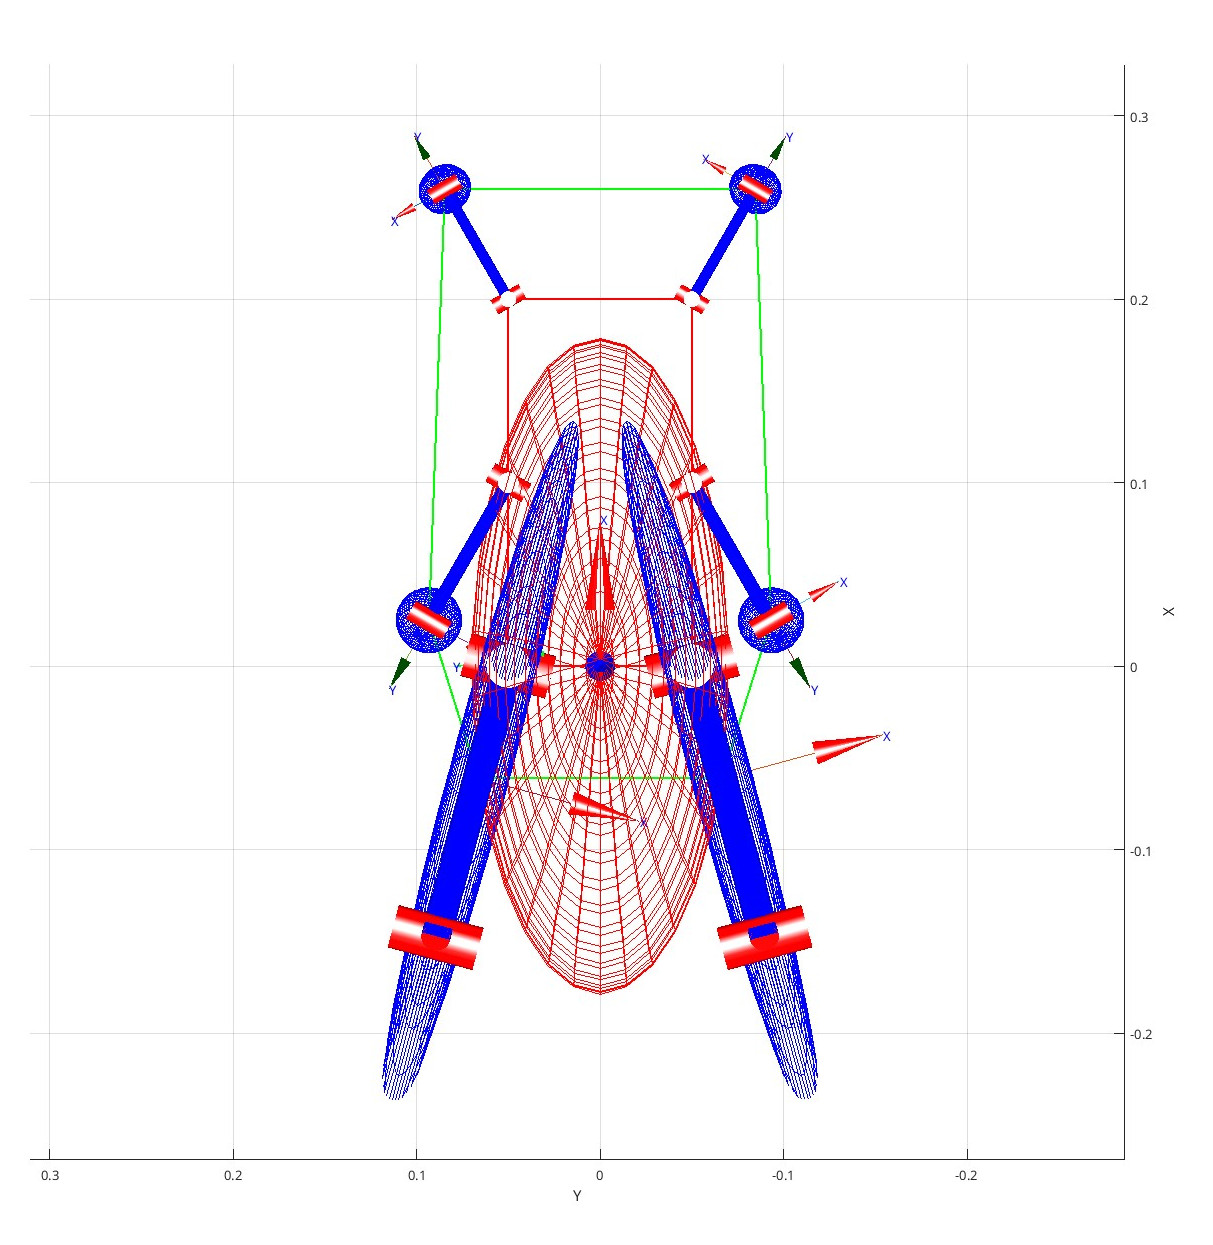
\includegraphics[width=0.4\textwidth]{Images/img_ch3/jumping_CoM_0_xy.jpg}}
    \subfloat[xz view\label{fig:jumping_CoM_0_xy}]
    {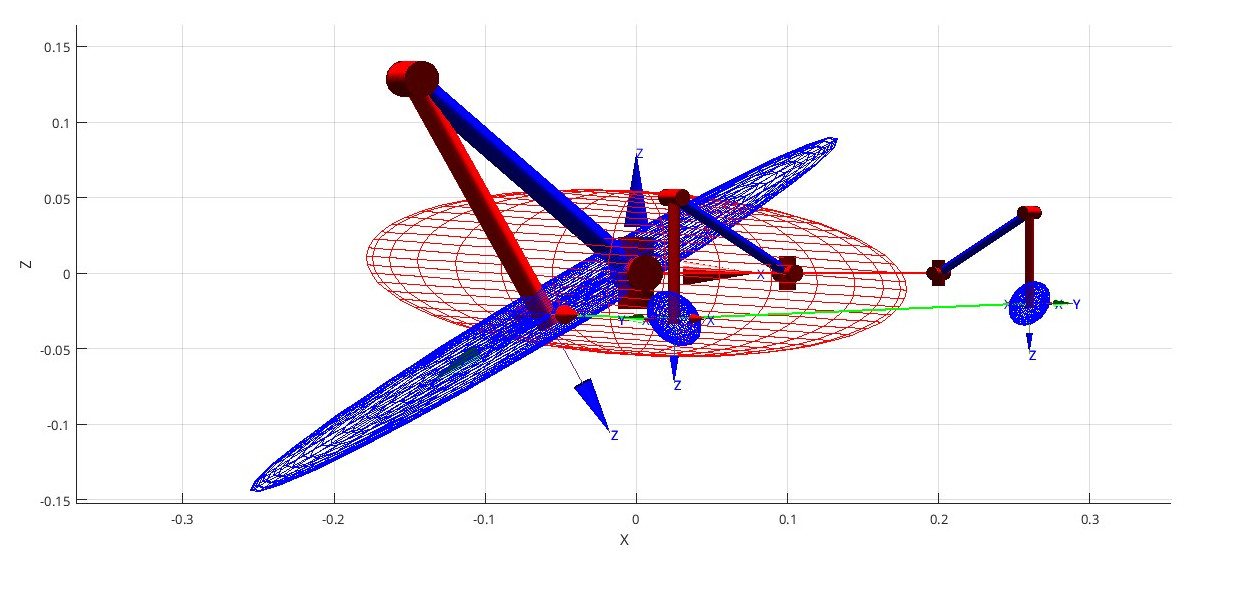
\includegraphics[width=0.4\textwidth]{Images/img_ch3/jumping_CoM_0_xz.jpg}}
    \caption[Jumping with different CoM]{Jumping with the CoM in the midpoint of the back legs}
    \label{fig:CoM_changes}
\end{figure}


\subsection{Final Comments on Multi-Limb robot base ME}
\label{sec:Conclusions}

The results of the examples above prove that the ATBVME is an intuitive and powerful geometrical tool, to identify the preferred direction of base motion. The ellipsoids obtained in all the configurations are consistent with the one expected by an extension of the original theory. Unfortunately, some of the limitations of the manipulability theory are reflected here, and in some cases, even if the shape is correct, the dimensions are just indicative and possibly misleading. 

For this reason, in the current formulation, this theory is useful to estimate directions with good mobility, but not accurate for defining quantitative indices to optimize. 
The scaling approach used for the grasshopper example has been tested also in LimbedEx1 and LimbedEx2, obtaining more meaningful ellipsoid axis ratios, but still high volume in inefficient configurations. 

Nevertheless, this approach is useful for multi-limbed robots with complex limb designs, characterized by unexpected possible base motion, identifiable using the major axis of the ATBVME. For this reason, it will be used to analyze the mobility of the robotic system used in this research and introduced in the following chapter, LIMBERO-GRIEEL.




\clearpage
\thispagestyle{empty} % This removes the header/footer but keeps the numbering
\vspace*{\fill} % Pushes everything to the bottom
\newpage
\BlankPageTLGWtwo
\chapter{LIMBERO-GRIEEL, Hardware and Software}
\label{ch:chapter_four}%

In this chapter, LIMBERO-GRIEEL, the robotic system used for this research is presented. Defining its configuration is important to understand its purpose and the problems addressed in the next chapters. 

\textbf{LIMBERO} (\textbf{LIMB}-climbing \textbf{E}xploration \textbf{RO}bot) is a prototype omnidirectional four-limbed robot, designed, 3D printed, and assembled by the Limb Team at the Space Robotics Lab \cite{SRL}(SRL) (led by Professor Yoshida Kazuya at Tohoku University, Japan). It is a small lightweight climbing robot, with a claw-type gripper\cite{passiveSpineTohoku} in its default design.\\
\textbf{GRIEEL} (\textbf{GRI}pper wh\textbf{EEL}) is a prototype gripper-wheel transformable mechanism, designed and patented by Masahiro Uda \textit{est all}\cite{GrieelUda}\cite{GRIEELUdaThesis}, member of the SRL Rover Team.  

\textbf{LIMEBRO-GRIEEL} is obtained from the assembly of the two systems described above, enabling wheeled locomotion in addition to walking and climbing. 
The overall system used in this research is still in the early stages of development, and a new version of GRIEEL (here referred to as GRIEELv2) has been already developed, as new limbs for LIMBERO-GRIEELv2. 
Chapter \ref{ch:chapter_nine} presents briefly these new versions of the prototypes. 

The robotic structure used during this research is described in terms of its hardware structure and the ROS2 control software architecture. Then, the Gazebo and MATLAB-Simulink simulation is briefly described, the first used to validate the motion control software and the additional algorithm implemented (described in chapter \ref{ch:chapter_five}), the second to tune the joints controllers and analyze the base manipulability ellipsoid, described in the previous chapter. 

\newpage 

\section{Hardware Description}
\label{sec:hardware}

The Hardware is described in this section, first with an overview of the limb structure and its actuated joints, and an explanation of how the gripper-wheel mechanism works and what are the two main mode configurations. Finally, the servo motors used to control the joints are listed.   

\subsection{Limb Description}
\label{sec:limb}
In its current design, LIMBERO is an omnidirectional quadruped with $4-DOF$ insect leg topology (different legs' views are represented in Fig.\ref{fig:LIMBERO_limb}) \cite{Todd}\cite{LeggedRObotBiomechanics}\cite{ReviewLegged}, in particular the choice of this structure comes from the studies of Kentaro Uno on HubRobo \cite{HubRobo}. 
In his PhD dissertation \cite{KentaroUnoPhD}, he proved that for climbing locomotion, the insect configuration results in
being more stable, energy-efficient, and versatile at once.


GRIEEL is the transformable end effector module (represented in Fig.\ref{fig:Gripper_Wheel}), but here this name is used to refer to the overall actuated mechanism, composed of the module and a $3-DOF$ mounting mechanism used for limb attachment, configuration change, and driving locomotion \cite{GRIEELUdaThesis} (represented in Fig.\ref{fig:GRIEEL_GRIPPER_WHEEL}).   


\begin{figure}[H]
    \centering
    \subfloat[\label{fig:Limbero_sideVIEW2}]{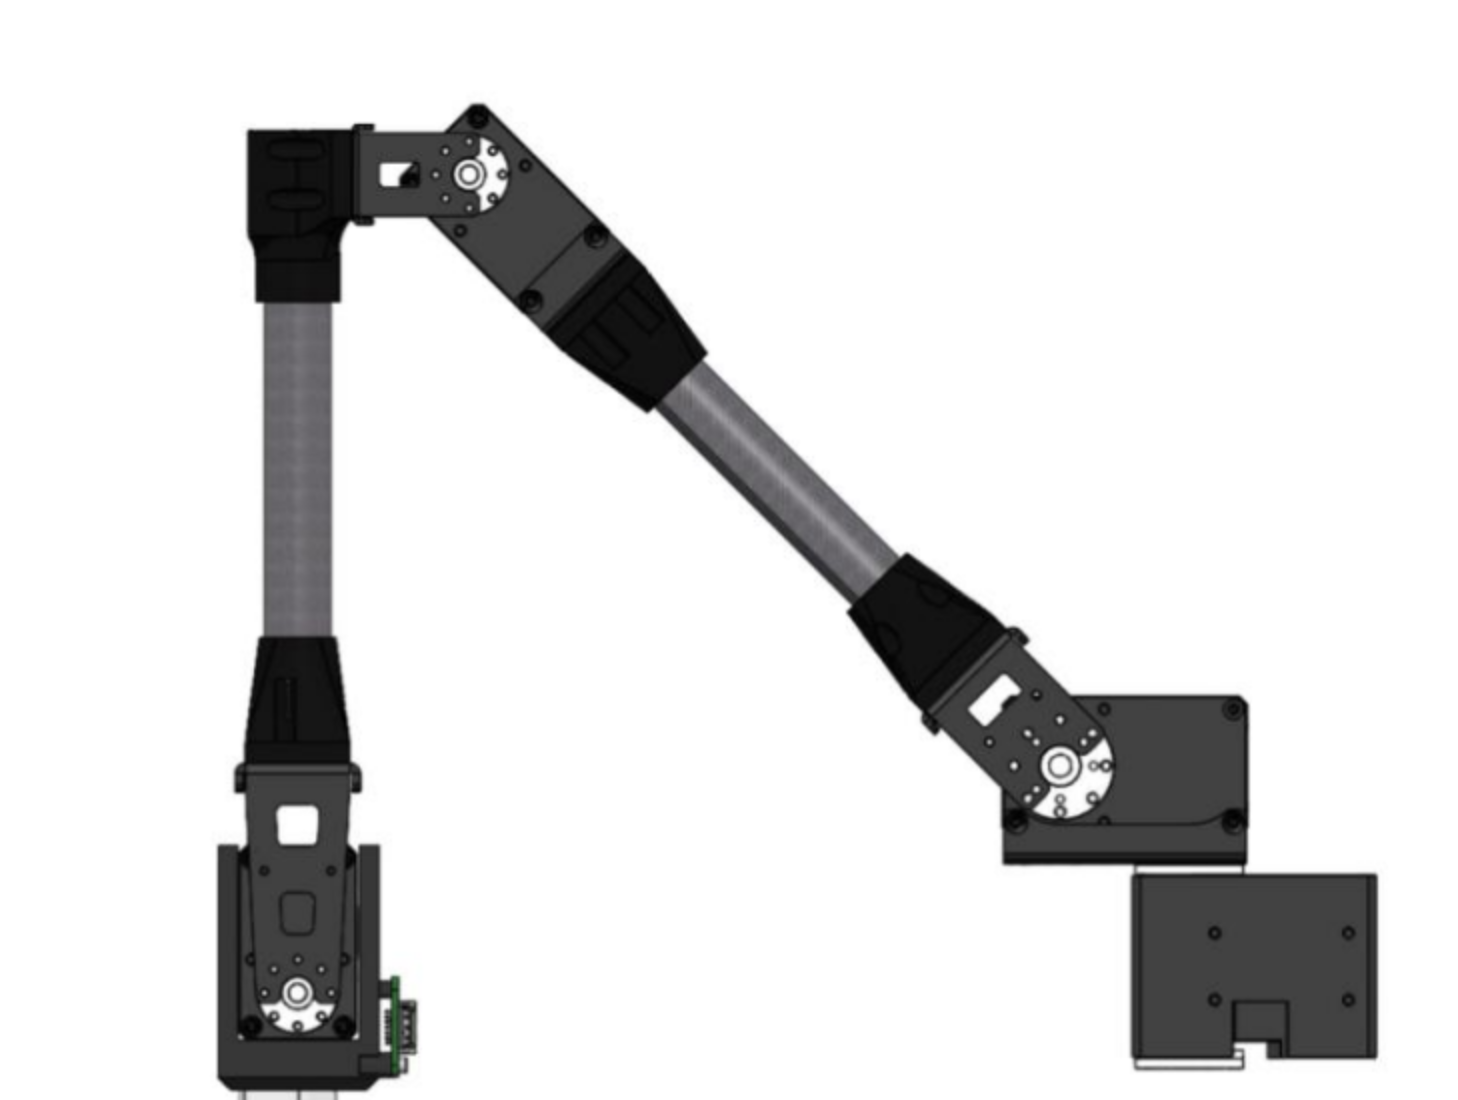
\includegraphics[scale=0.1]{Images/img_ch4/limbero_sideVIEW2.png}}
    \subfloat[\label{fig:Limbero_orthoVIEW}]{\includegraphics[scale=0.1]{Images/img_ch4/Limbero_orthoVIEW.png}}\\
    \subfloat[\label{fig:Limbero_sideVIEW1}]{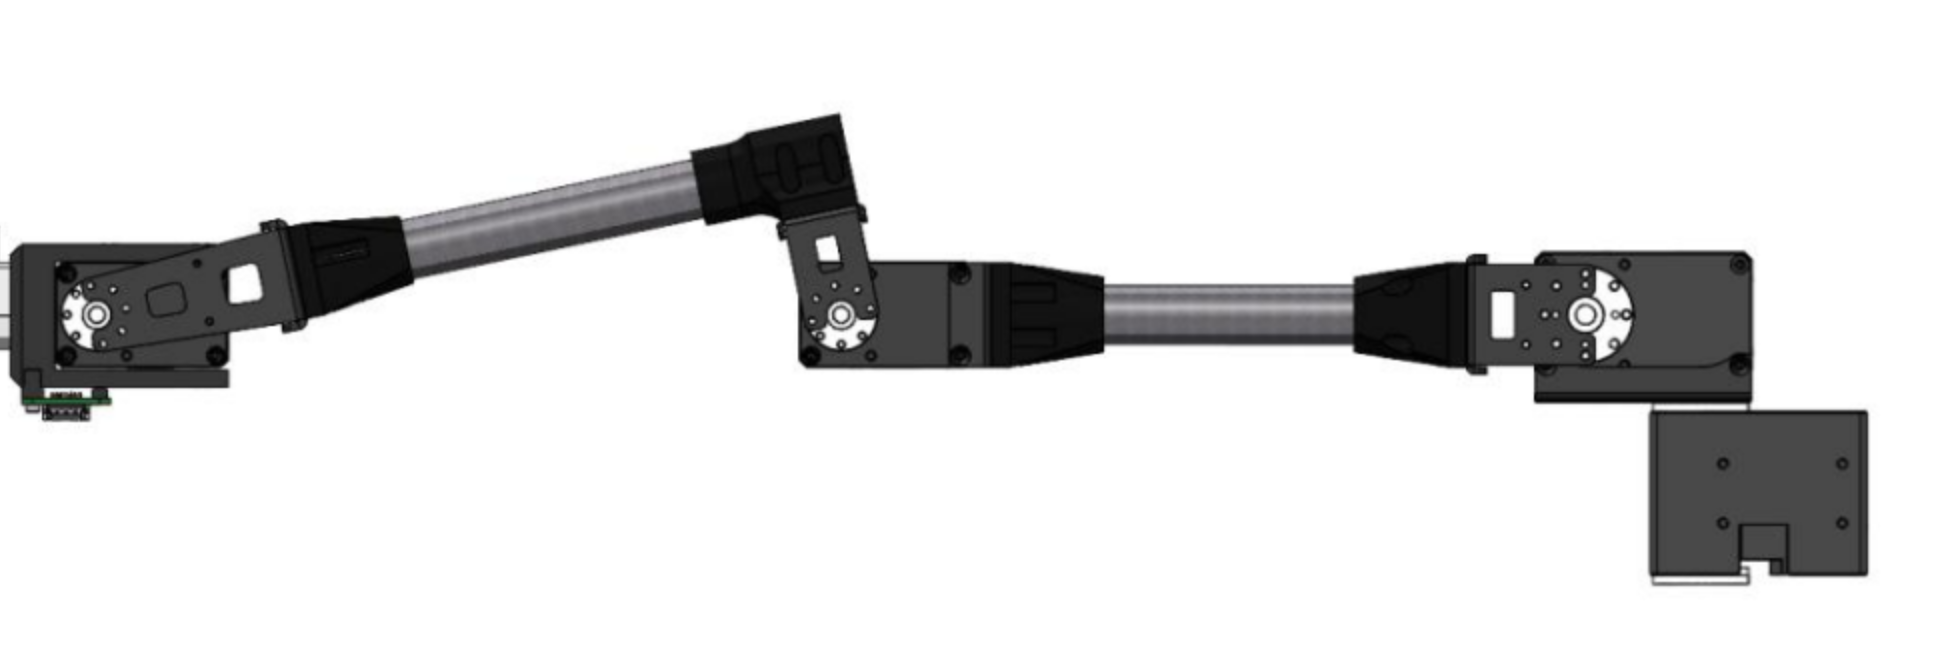
\includegraphics[scale=0.1]{Images/img_ch4/limbero_sideVIEW1.png}}
    \caption[Different views of LIMERO limb model]{\cite{LIMBEROTakadaThesis} Views of LIMERO limb model, without the claw-type gripper EE, (a) and (b) are in the same configuration, while (c) is in the zero joints configuration}
    \label{fig:LIMBERO_limb}
\end{figure}

\begin{figure}[H]
    \centering
    \subfloat[Gripper-Wheel module.\label{fig:Gripper_Wheel}]{\includegraphics[scale=0.20]{Images/img_ch4/Gripper_Wheel.png}}
    \\
    \subfloat[actuated GRIEEL mechanism in the two modes.\label{fig:GRIEEL_GRIPPER_WHEEL}]{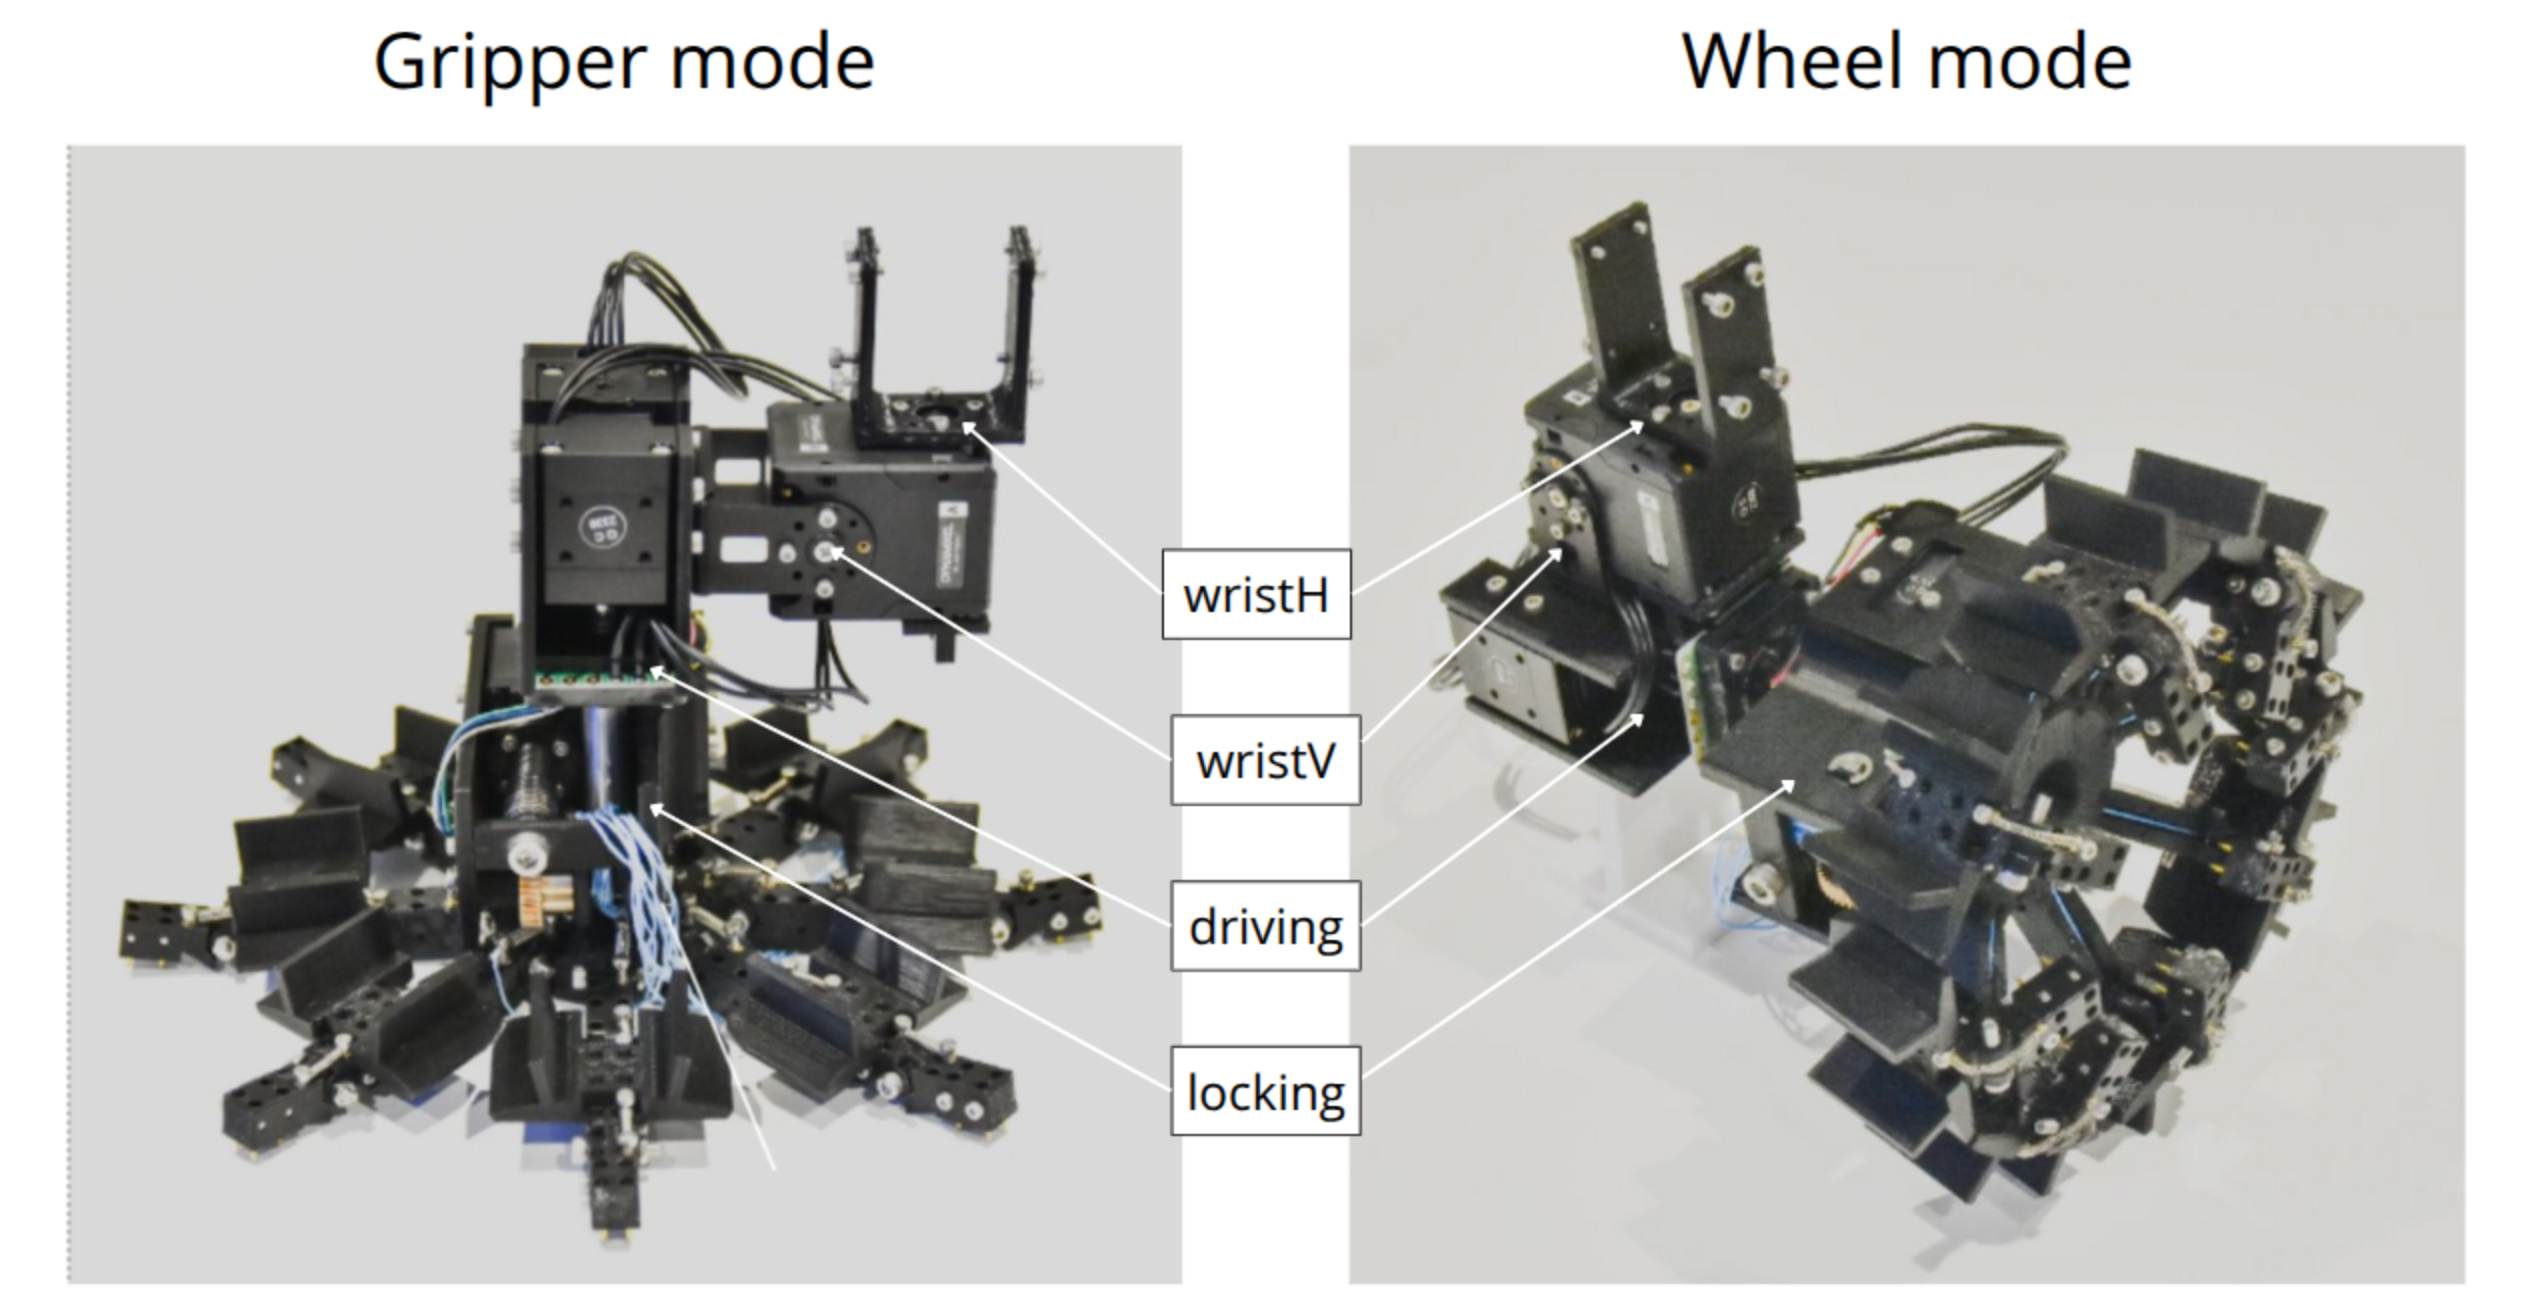
\includegraphics[scale=0.15]{Images/img_ch4/GRIEEL_GRIPPER_WHEEL.png}}
    \caption[GRIEEL module and actuation mechanism]{GRIEEL module and actuation mechanism}
    \label{fig:GRIEELMechanism}
\end{figure}

The assembled limb structure, with its $7-DOF$ is a redundant system on the 6-dimensional position and orientation task space of its limb tip  (the model and the real limb are represented in Fig.\ref{fig:LIMBERO_GRIEEL_limb}, and the equivalent schematic model in Fig.\ref{fig:LIMBERO_GRIEEL_limb_model}). 
Introducing some names, with the notation introduced in chapter \ref{sec:kinematic}, the set of limbs here defined as $J = \{LF, LH, RH, RF \}$ (Left Front, Left Hind, Right Hind and Right Front), and the joint space of each limb $\mathbf{q}_j \in \mathbb{R}^7, \forall j\in J $, where the joints have the following names:\\
$q_{j,i} \in \{ j\_B2C, j\_C2F,  j\_F2T, j\_T2E,j\_wristH, j\_wristV, j\_driving\}$, as ordered in the serial kinematic structure. The names of the joints come from a common naming convention for the limb links in walking robots, for LIMBERO ordered as {limb\_root, coxa, femur, tibia, limb\_end}  and with a wrist notation for GRIEEL {wristH(orizontal), wristV(ertical), driving, gripper/wheel}.
The overall structure of the links' interconnection is represented in Fig.\ref{fig:TFTree_NOFINGERS} below.  
 
\begin{figure}[H]
    \centering
    \subfloat[Side view in gripper mode.\label{fig:LIMBERO_GRIEEL_GRIPPER_side}]{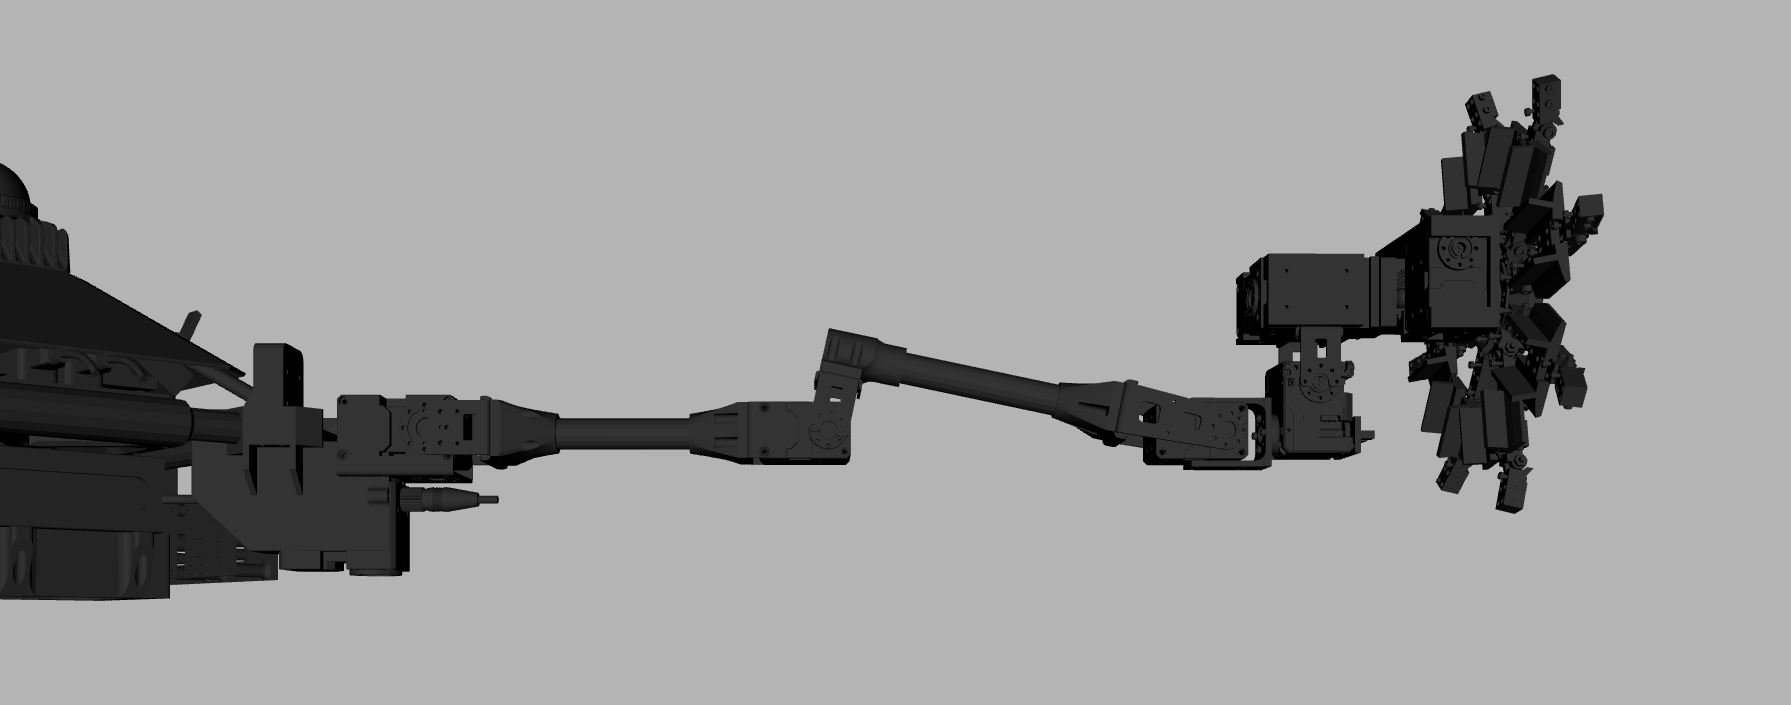
\includegraphics[width=0.4\textwidth]{Images/img_ch4/LIMBERO_GRIEEL_GRIPPER_side.png}}  \quad \subfloat[Side view in wheel mode.\label{fig:LIMBERO_GRIEEL_WHEEL_side}]{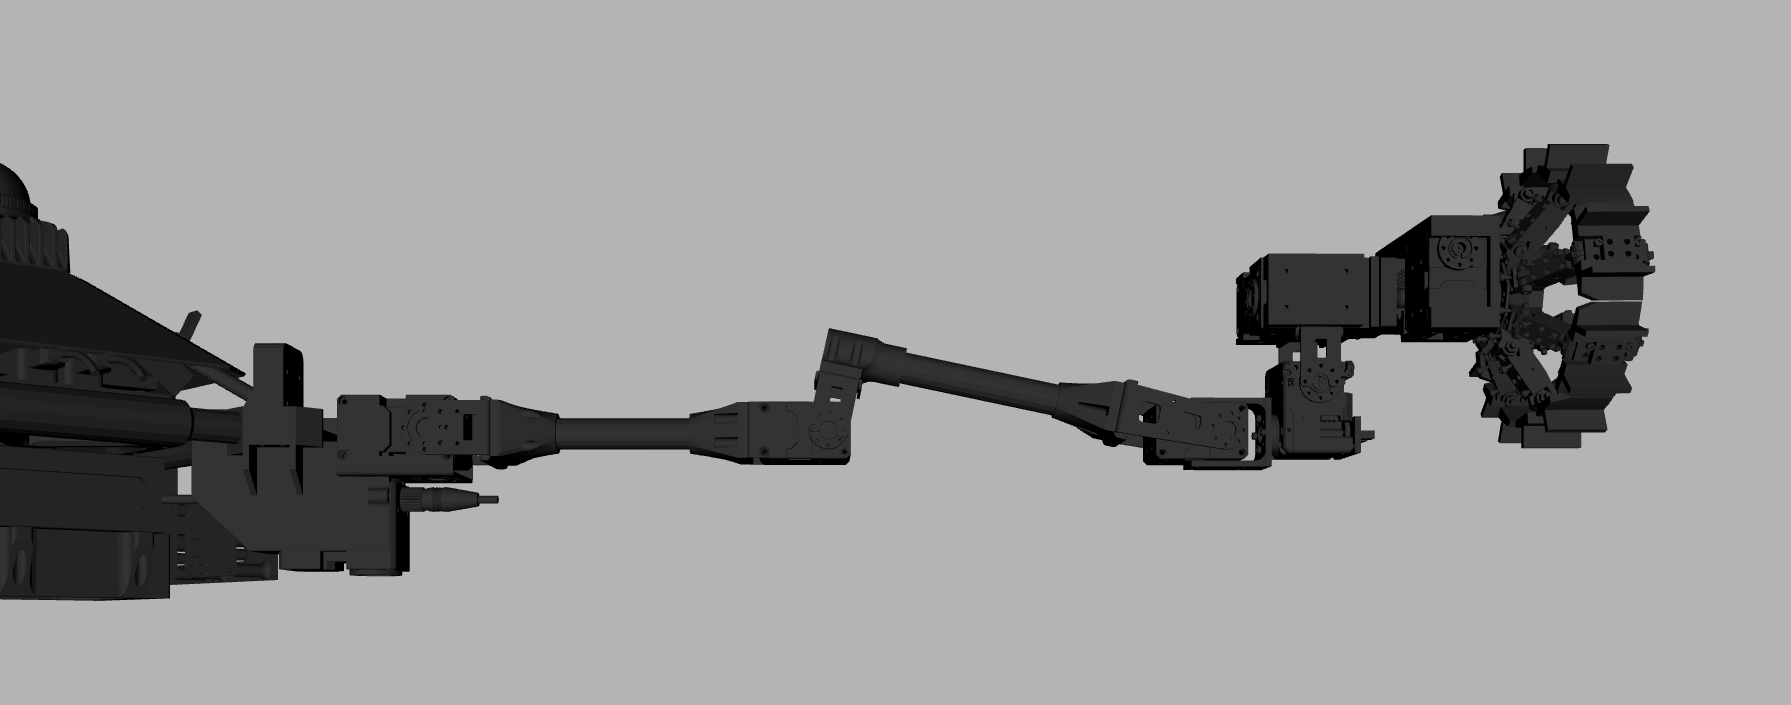
\includegraphics[width=0.4\textwidth]{Images/img_ch4/LIMBERO_GRIEEL_WHEEL_side.png}}
    \\
    \subfloat[Top view in gripper mode.\label{fig:LIMBERO_GRIEEL_GRIPPER_top}]{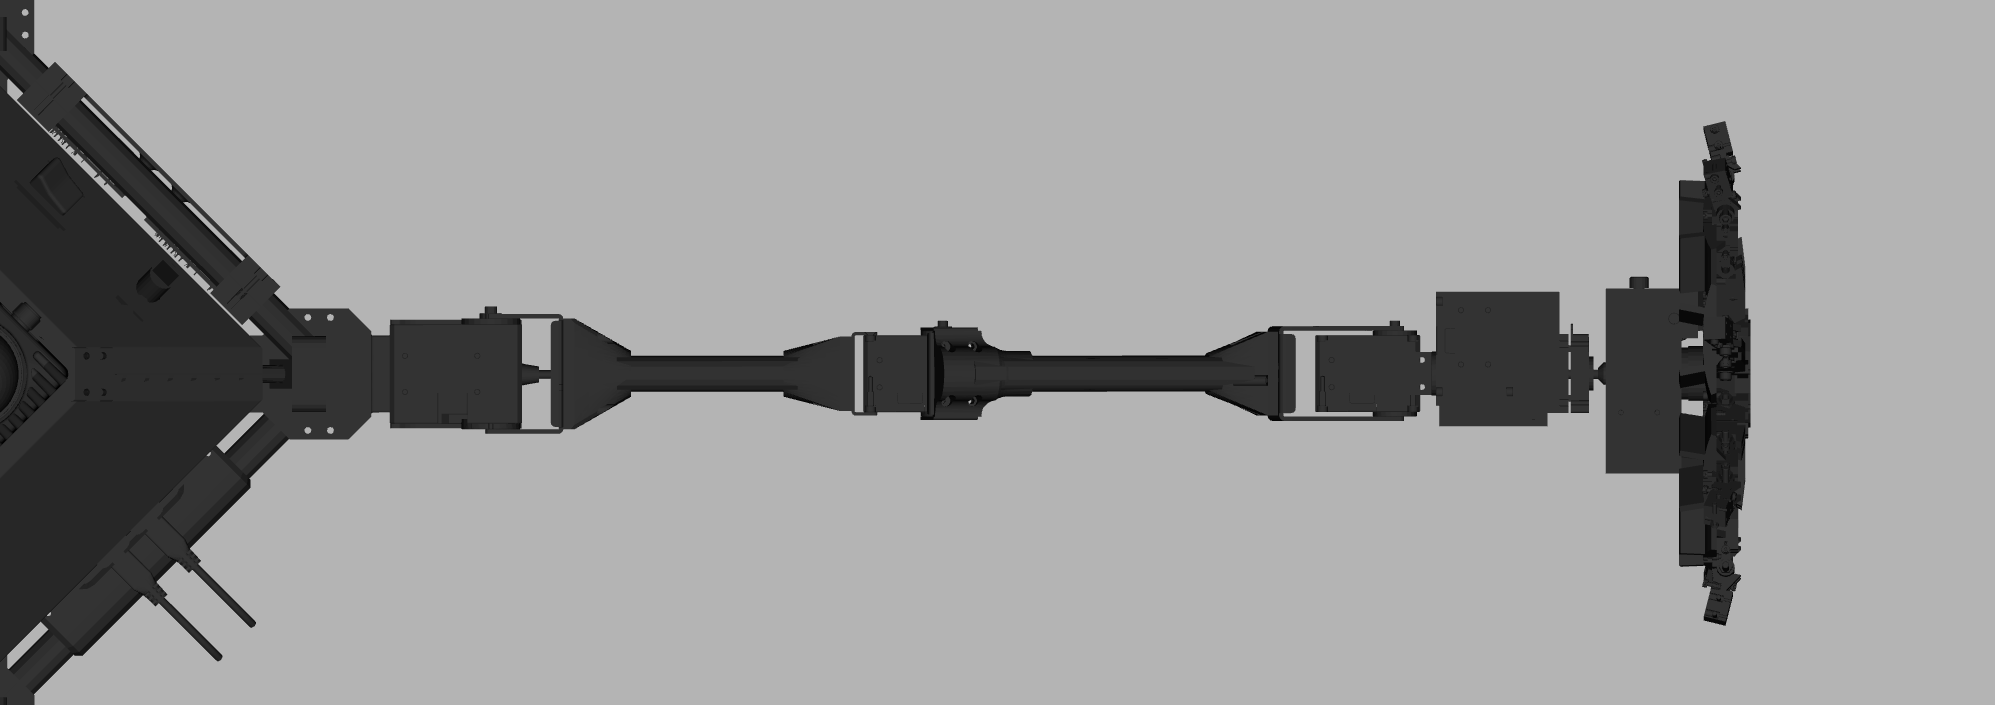
\includegraphics[width=0.4\textwidth]{Images/img_ch4/LIMBERO_GRIEEL_GRIPPER_top.png}}   \quad
    \subfloat[Top view in wheel mode.\label{fig:LIMBERO_GRIEEL_WHEEL_top}]{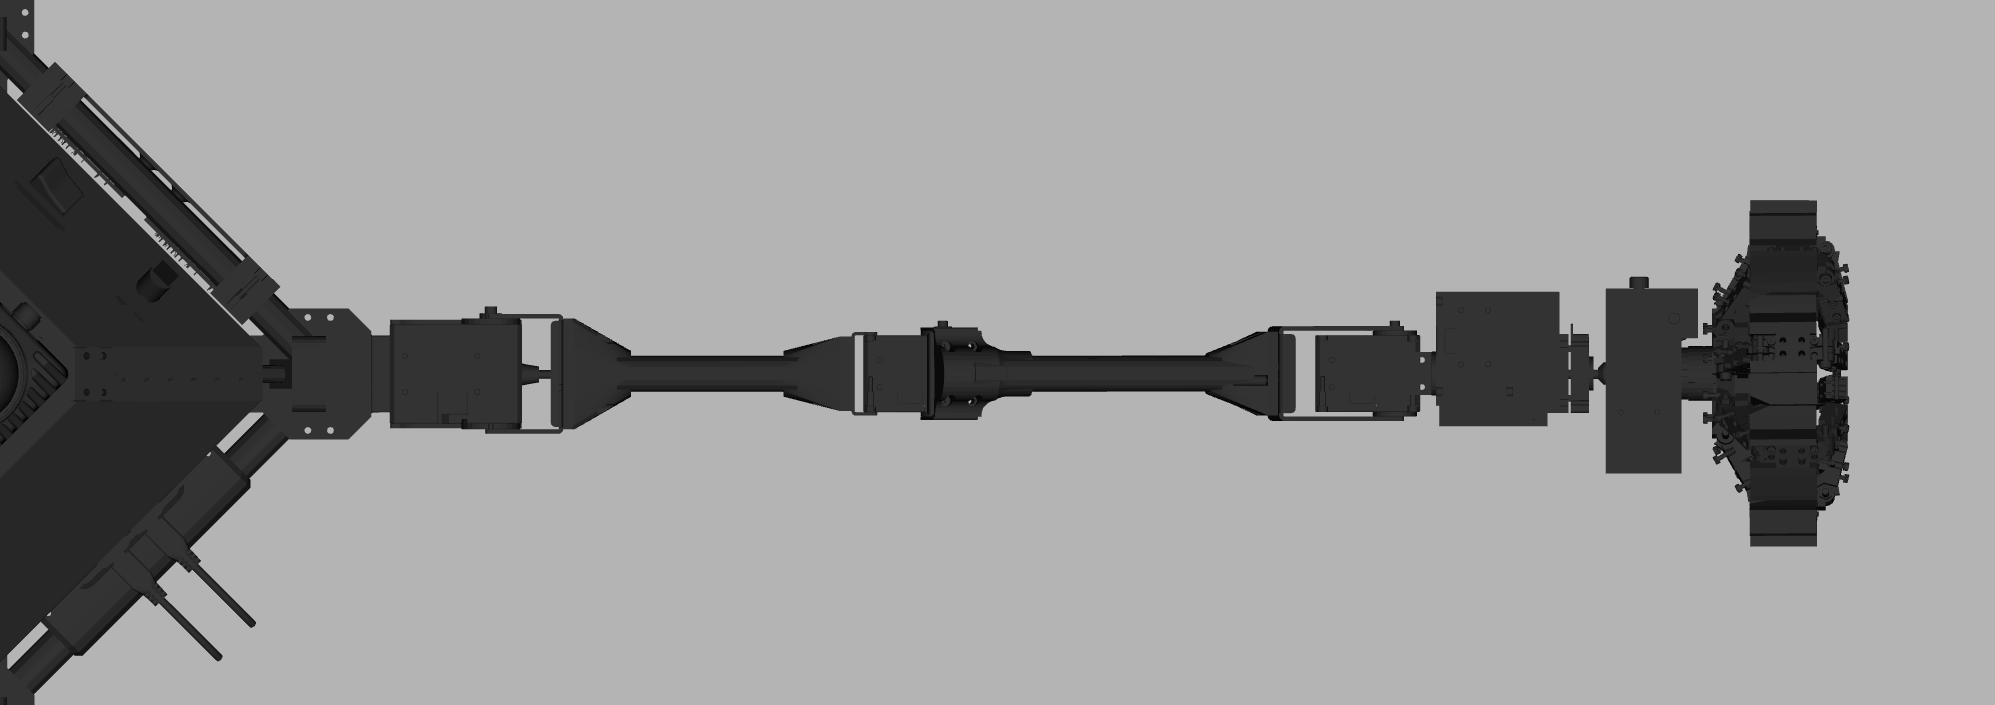
\includegraphics[width=0.4\textwidth]{Images/img_ch4/LIMBERO_GRIEEL_WHEEL_top.png}}
    \\
    \subfloat[Perspective view in gripper mode.\label{fig:LIMBERO_GRIEEL_GRIPPER_ortho}]{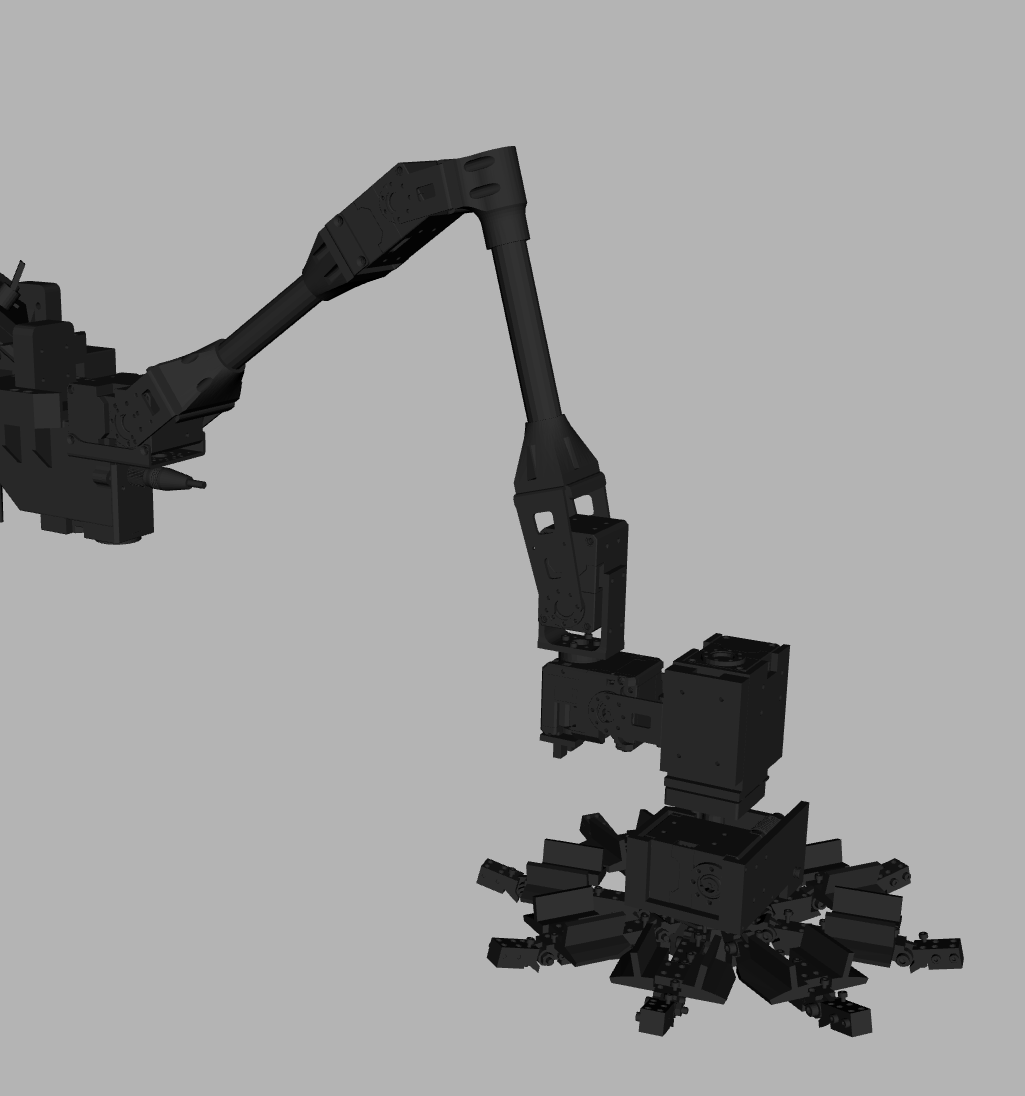
\includegraphics[width=0.4\textwidth]{Images/img_ch4/LIMBERO_GRIEEL_GRIPPER_ortho.png}}   \quad\subfloat[Perspective view in wheel mode.\label{fig:LIMBERO_GRIEEL_WHEEL_ortho}]{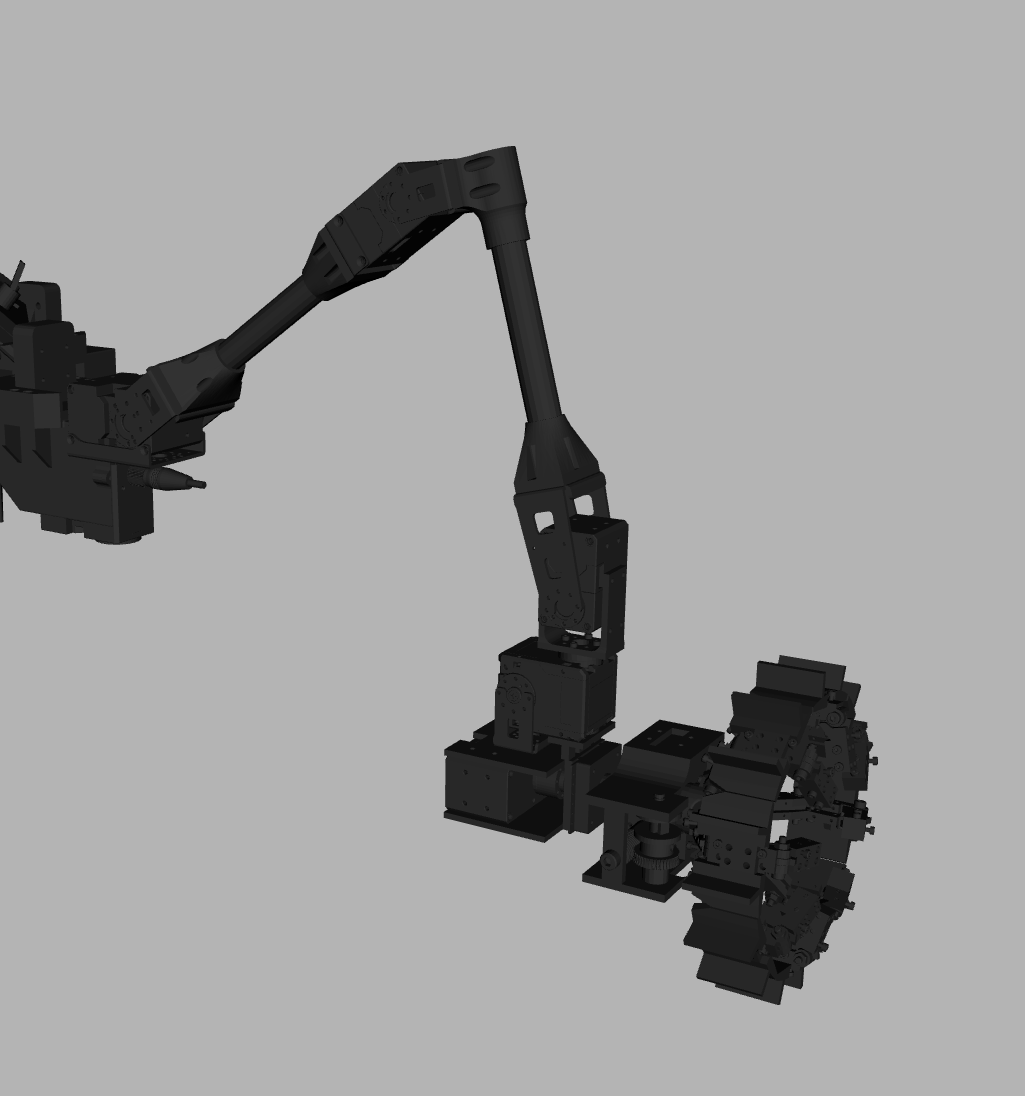
\includegraphics[width=0.4\textwidth]{Images/img_ch4/LIMBERO_GRIEEL_WHEEL_ortho.png}}
    \\
    \subfloat[Real limb in gripper mode. \label{fig:LIMBERO_GRIEEL_GRIPPER_hw}]{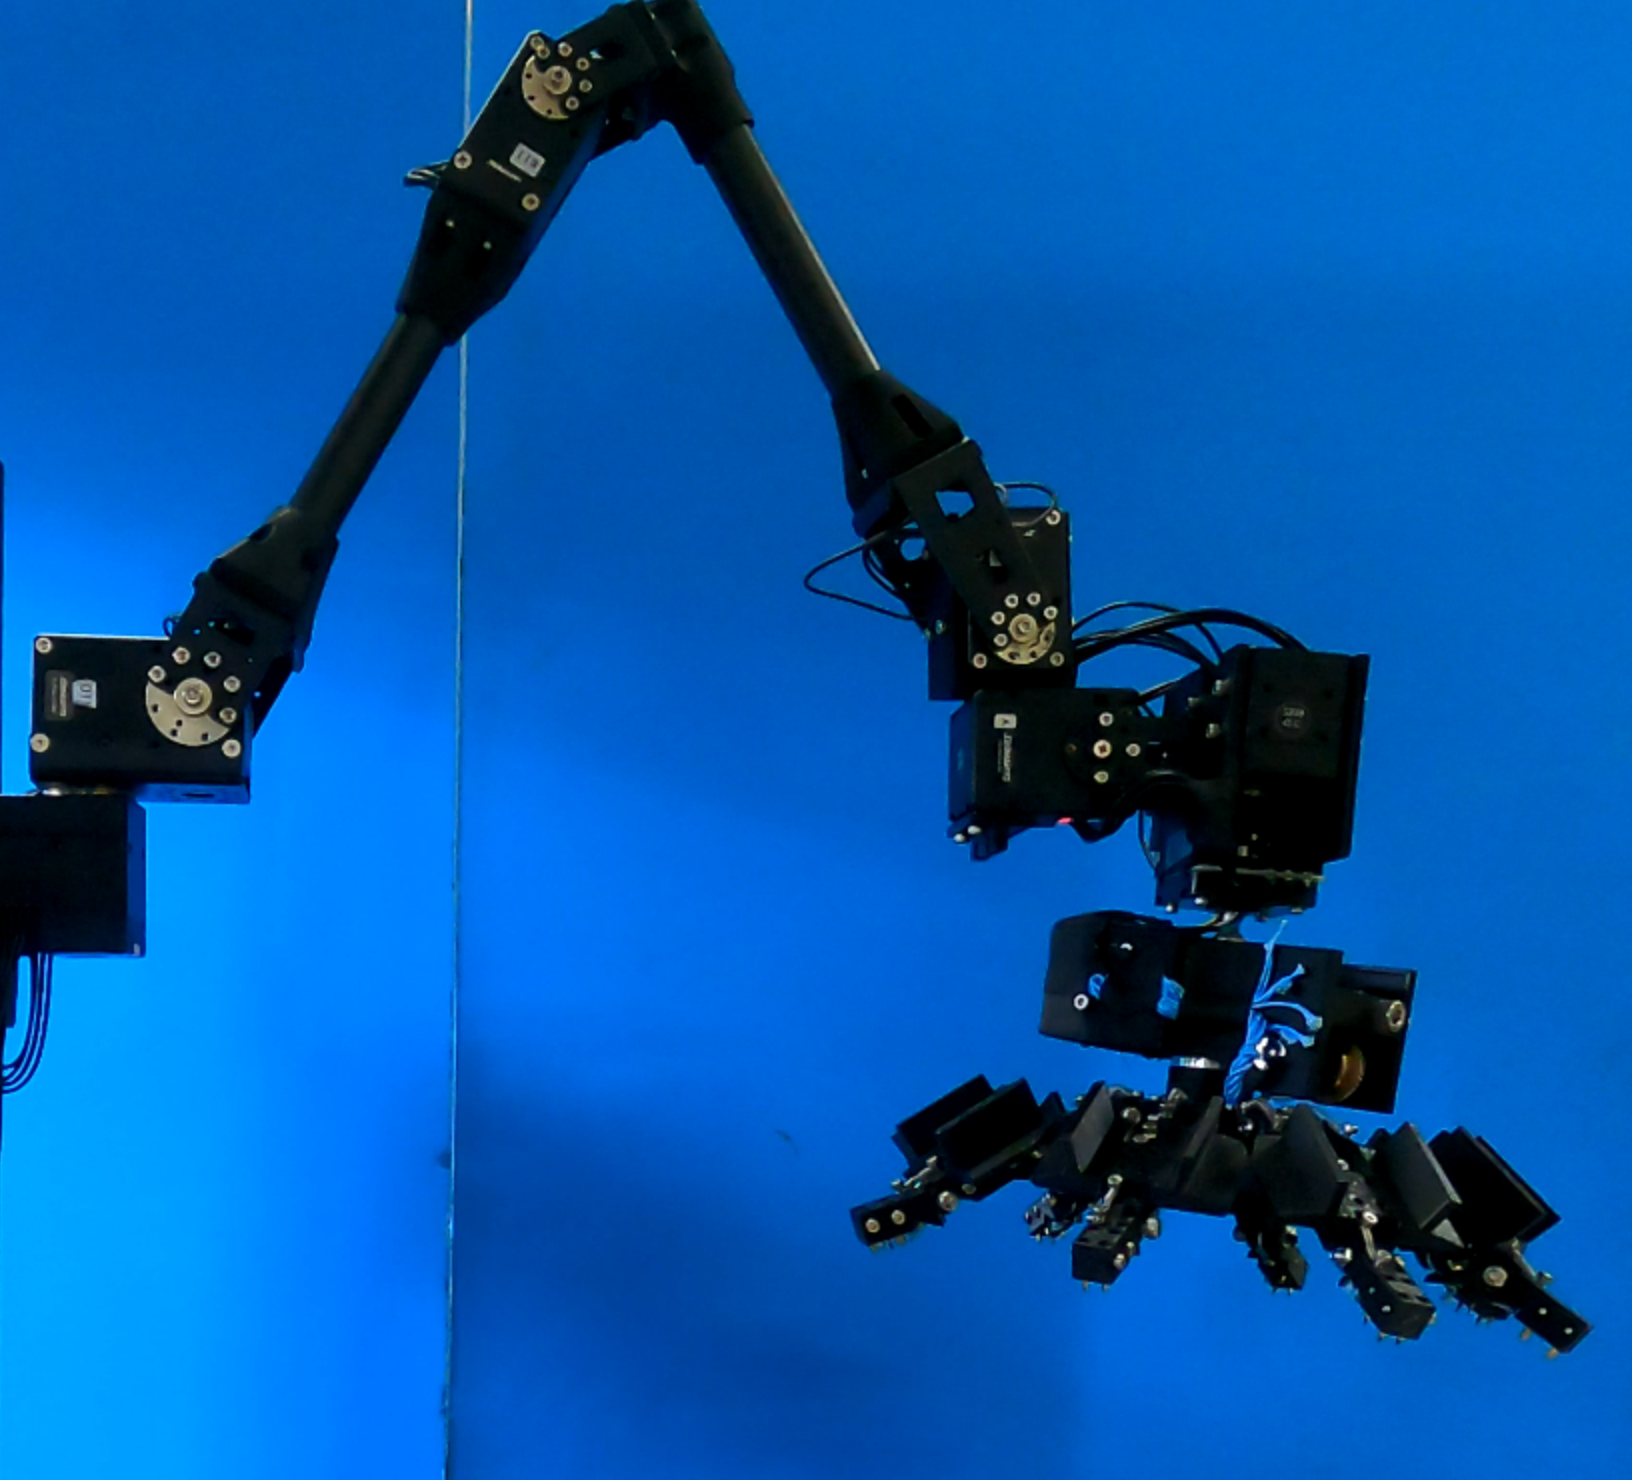
\includegraphics[width=0.4\textwidth]{Images/img_ch4/LIMBERO_GRIEEL_GRIPPER_hw.png}}   \quad\subfloat[Real limb in wheel mode.\label{fig:LIMBERO_GRIEEL_WHEEL_hs}]{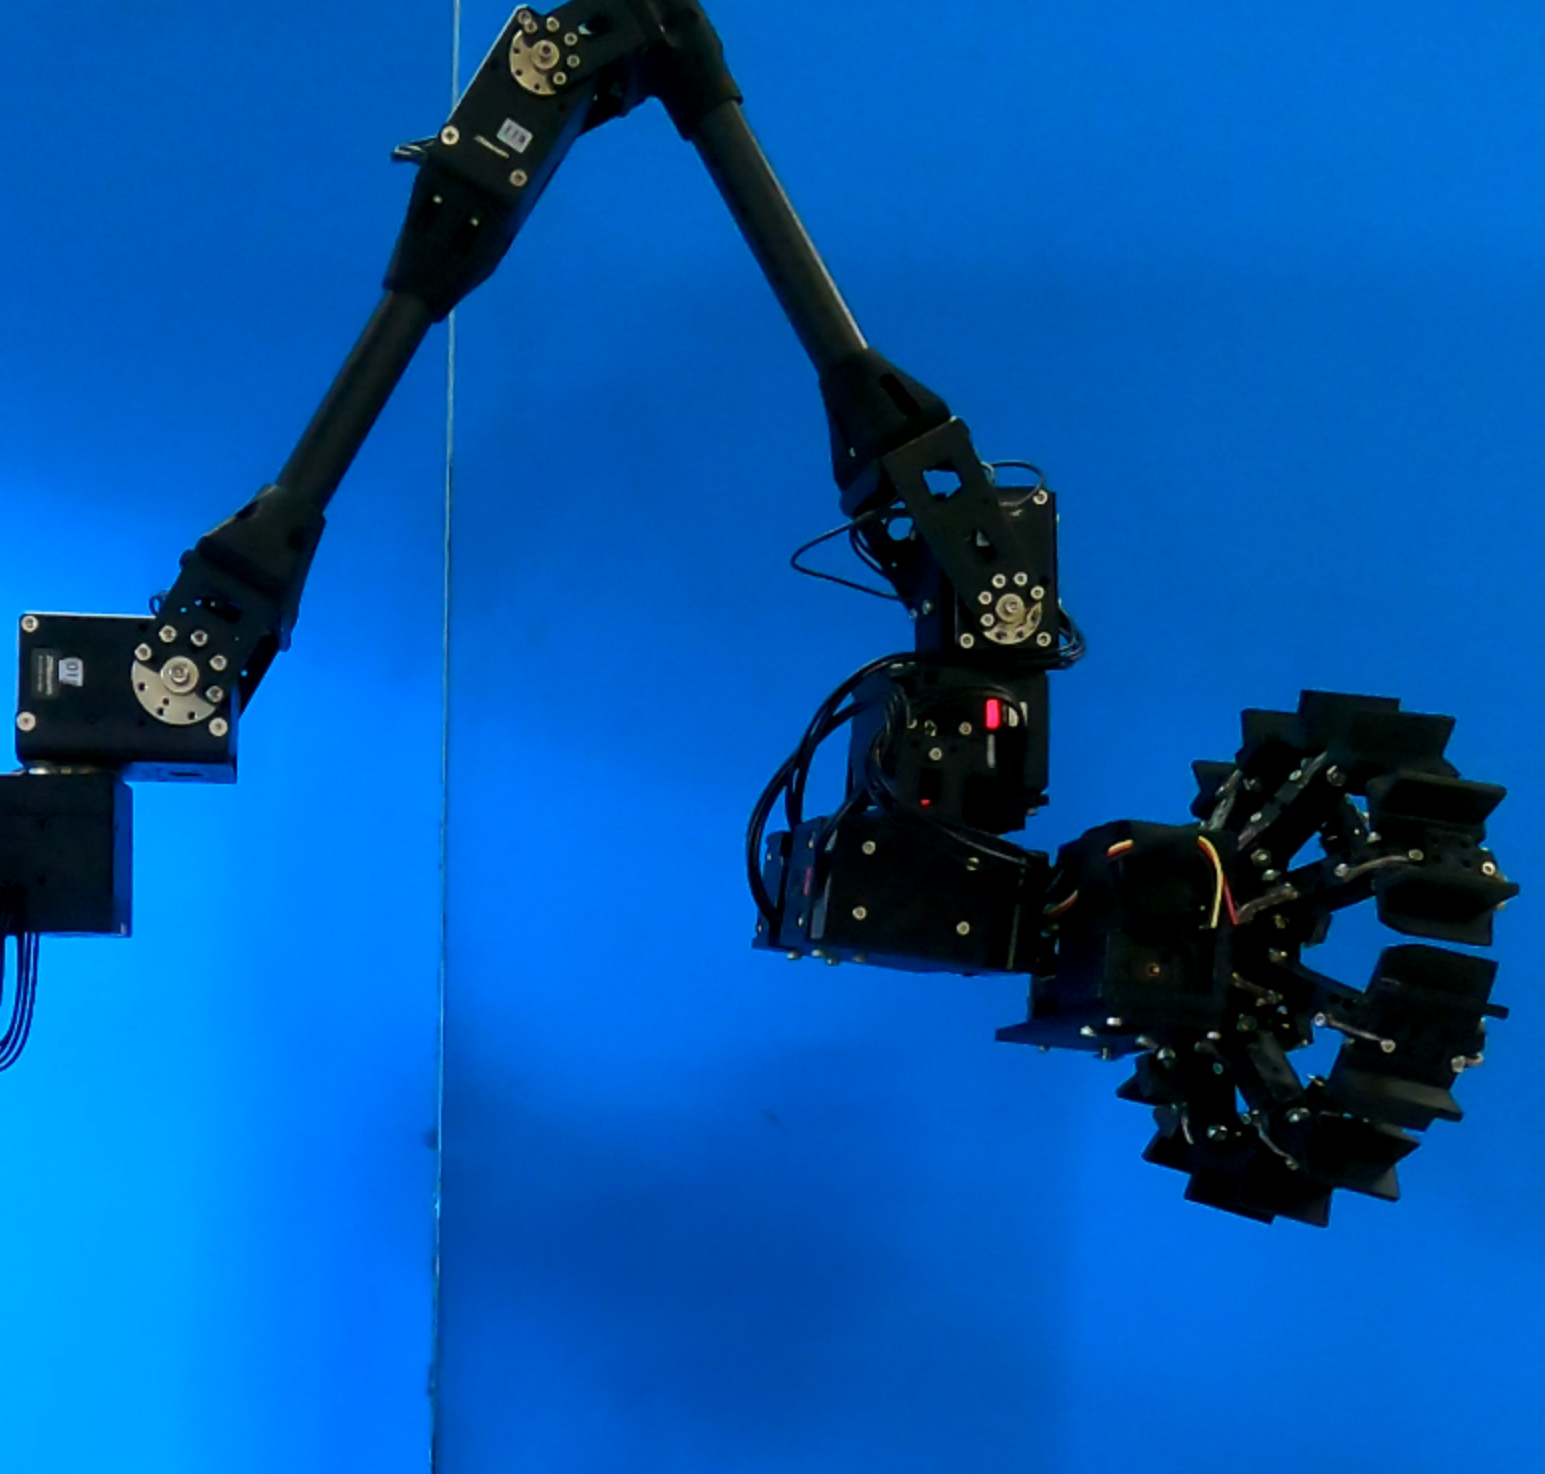
\includegraphics[width=0.4\textwidth]{Images/img_ch4/LIMBERO_GRIEEL_WHEEL_hw.png}}

    \caption[Different views of LIMBERO-GRIEEL limb model and real system]{Different views of LIMBERO-GRIEEL limb model and real system}
    \label{fig:LIMBERO_GRIEEL_limb}
\end{figure}

\begin{figure}[H]
    \centering
    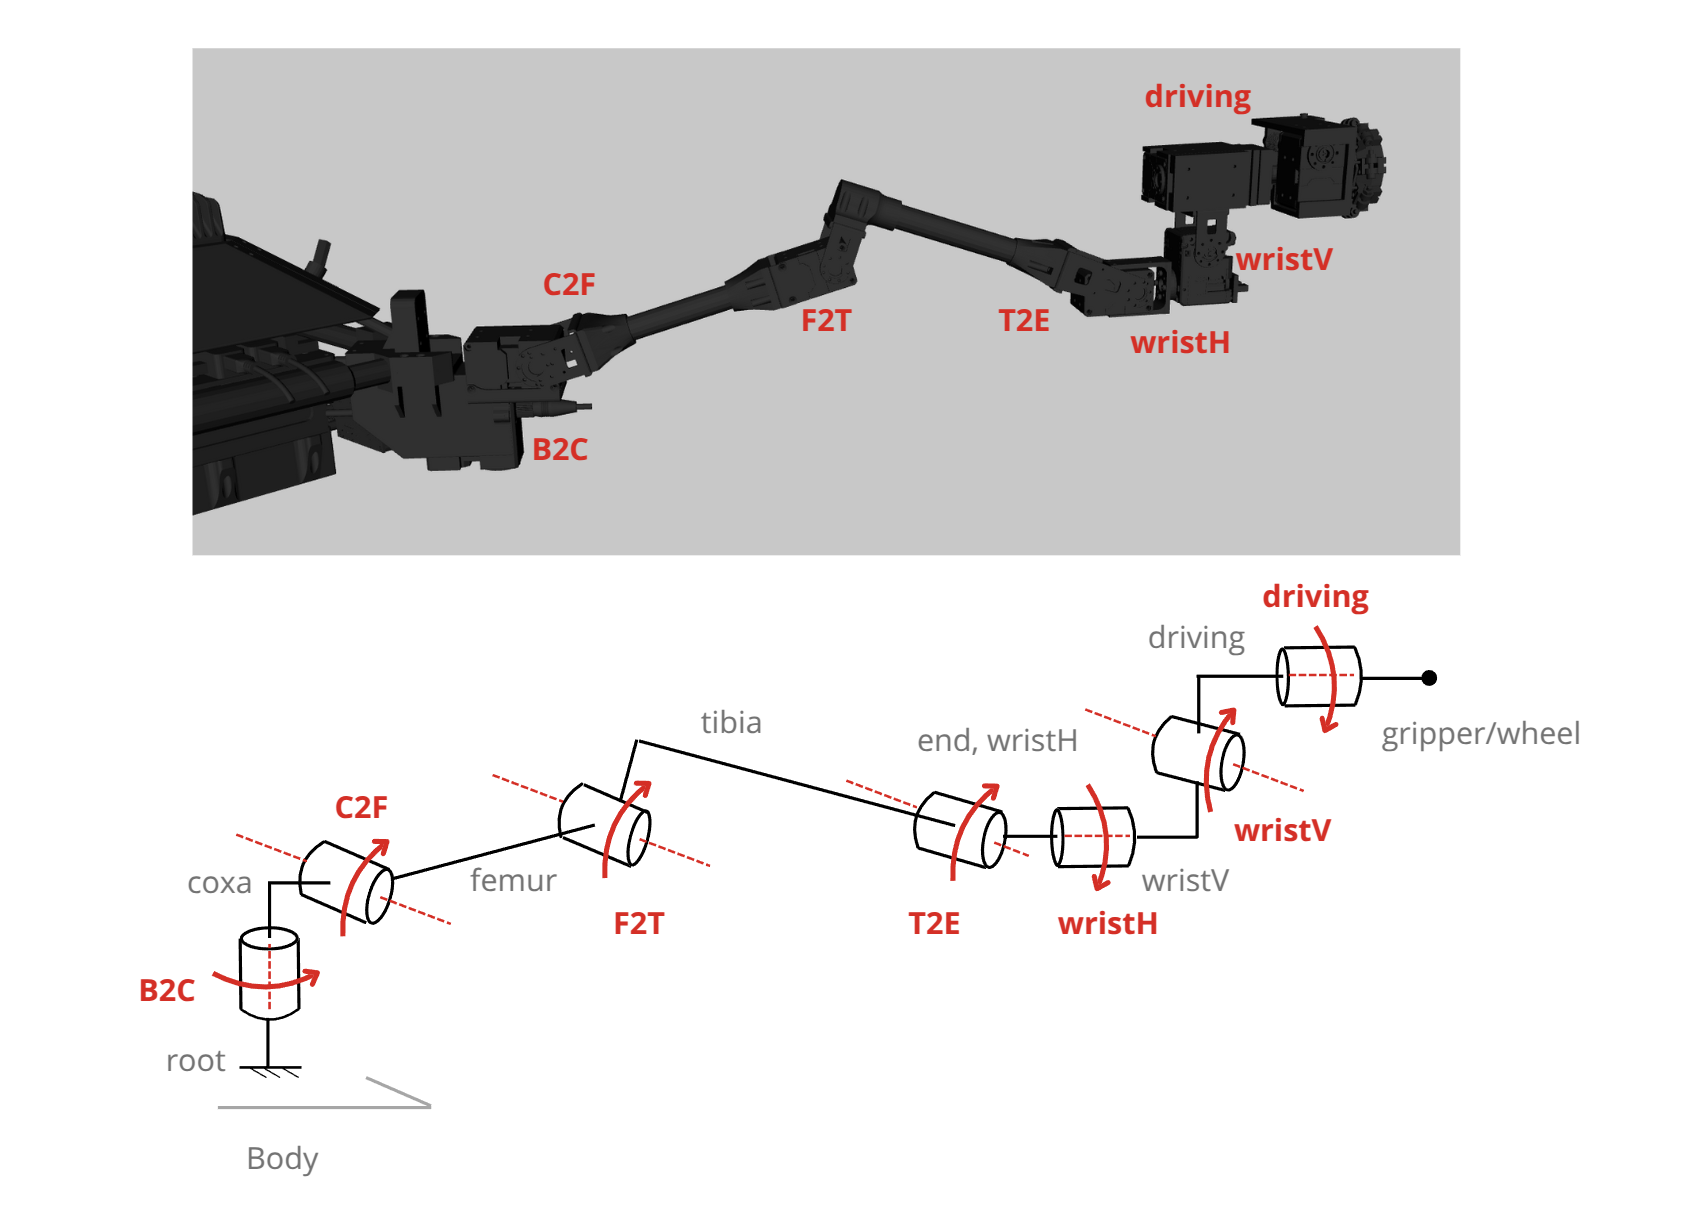
\includegraphics[width=1.0\textwidth]{Images/img_ch4/LIMBERO_GRIEEL_limb_model.png}
    \caption{Schematic model of actuated joints of LIMBERO-GRIEEL limb}
    \label{fig:LIMBERO_GRIEEL_limb_model}
\end{figure}

In principle, in the 3D translational/rotational task space this 7-DOFs structure is redundant, but as evident from the wheel mode, the \textit{driving} joint is included for wheeled locomotion. Therefore, in the motion tasks, the first six joints are used to control the pose, while the last when driving locomotion is required. However, in manipulation task, even when the module is used in gripper mode, the driving motor could be used to change the orientation of the manipulated object, which can be useful in some applications such as pick and place of samples.   

\begin{figure}[H]
    \centering
    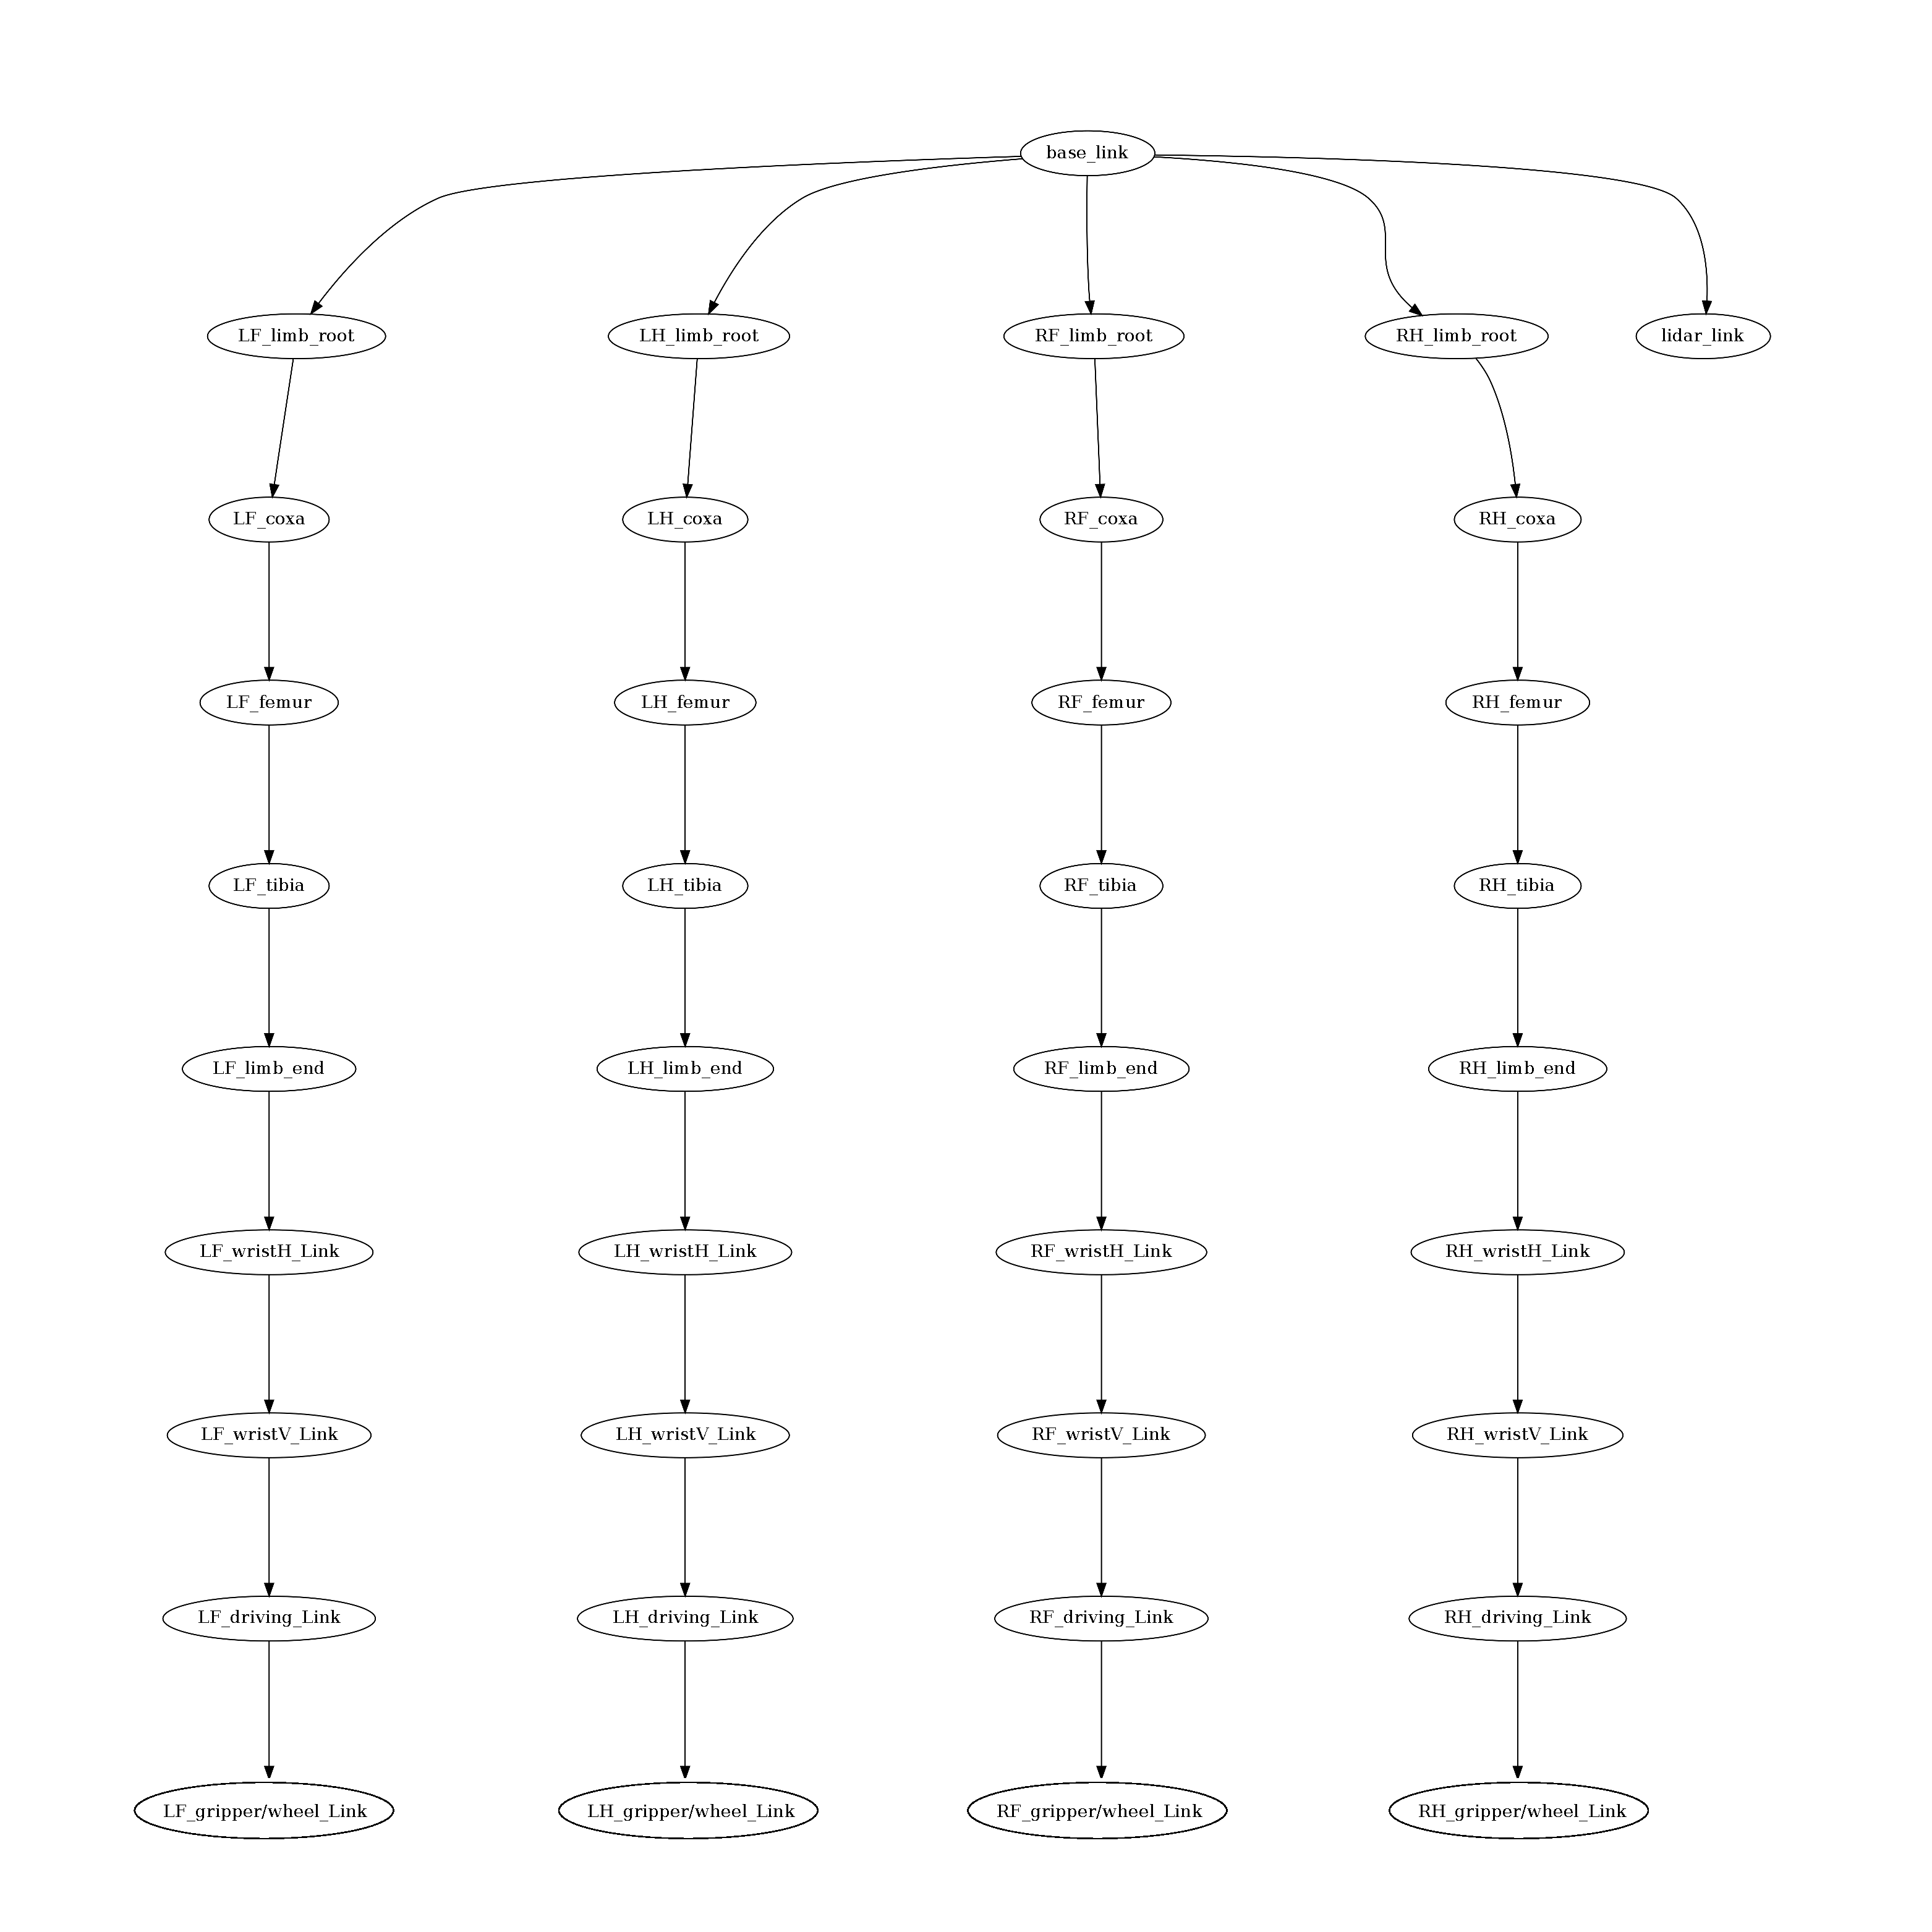
\includegraphics[width=1.0\textwidth]{Images/img_ch4/TFTree_NOFINGERS.pdf}
    \caption{Links structure of LIMBERO-GRIEEL Limb, neglecting gripper-wheel transformation fingers' joints}
    \label{fig:TFTree_NOFINGERS}
\end{figure}

Finally, the equivalent DH model of the limb is represented in Fig.\ref{fig:limbero_grieel_DH} (extracted from the robot Unified Robot Description Format (URDF), described in the software section), the DH parameters are reported in Tab.\ref{table:DH}, and the value of masses in Tab.\ref{table:Mass}.

\begin{table}[H]
\centering 
    \caption{LIMBERO-GRIEEL DH parameters}
    \label{table:DH}
    \begin{tabular}{| l | c | c | c | c | c |}
    \hline
    \rowcolor{bluepoli!40}
%    \rowcolor{bluepoli!40}
     \textbf{Link} &  $a_i$ $[m]$ & $\alpha_i$ $[rad]$ & $d_i$ $[m] $ & $\theta_i$ $[rad]$ & $\theta_{offset, i}$ $[rad]$ \T\B \\
    \hline \hline
    \textbf{coxa} ($i=1$) & 0.031 & $-\frac{\pi}{2}$ & 0.0  & $q_1$  & 0.0 \T\B\\
    \hline 
    \textbf{femur} ($i=2$) & 0.2 & 0.0  & 0.0  & $q_2$  & 0.0  \T\B\\
    \hline
    \textbf{tibia} ($i=3$) & 0.2  & 0.0  & 0.0  & $q_3$ & 0.0 \T\B\\
    \hline
    \textbf{limb-end} ($i=4$) & 0.0 &  $-\frac{\pi}{2}$ & 0.0 & $q_4$ &  $-\frac{\pi}{2}$  \B\\
    \hline
    \textbf{wristV} ($i=5$) & 0.024 &  $\frac{\pi}{2}$ & 0.0468 & $q_5$  & 0.0 \B\\
    \hline
    \textbf{driving} ($i=6$) & 0.0458  &  $-\frac{\pi}{2}$ & 0.0 & $q_6$  &  0.0 \B\\
    \hline
    \textbf{gripper/wheel} ($i=7$) & 0.0 & 0.0 & 0.1131 & $q_7$ & 0.0   \B\\
    \hline
    \end{tabular}

\end{table}

\begin{table}[H]
    \caption{LIMBERO-GRIEEL links masses}
    \label{table:Mass}
     \hspace{-2.0cm} % Adjust this value as needed
    \begin{tabular}{| c || l | l | l | l | l | l | l | l | l | l |}
    \hline
     \cellcolor{bluepoli!40}\textbf{Link} & body & root  & coxa & femur & tibia & limb-end & wristH & wristV & driving & G/W \T\B \\
    \hline 
    \cellcolor{bluepoli!40}\textbf{mass} [kg] & 3.115  & 0.085 & 0.091 &  0.128 & 0.062 & 0.082 & 0.008 & 0.102 & 0.133 & 0.416\T\B\\
    \hline 
    \end{tabular}
\end{table}

\begin{figure}[H]
    \centering
    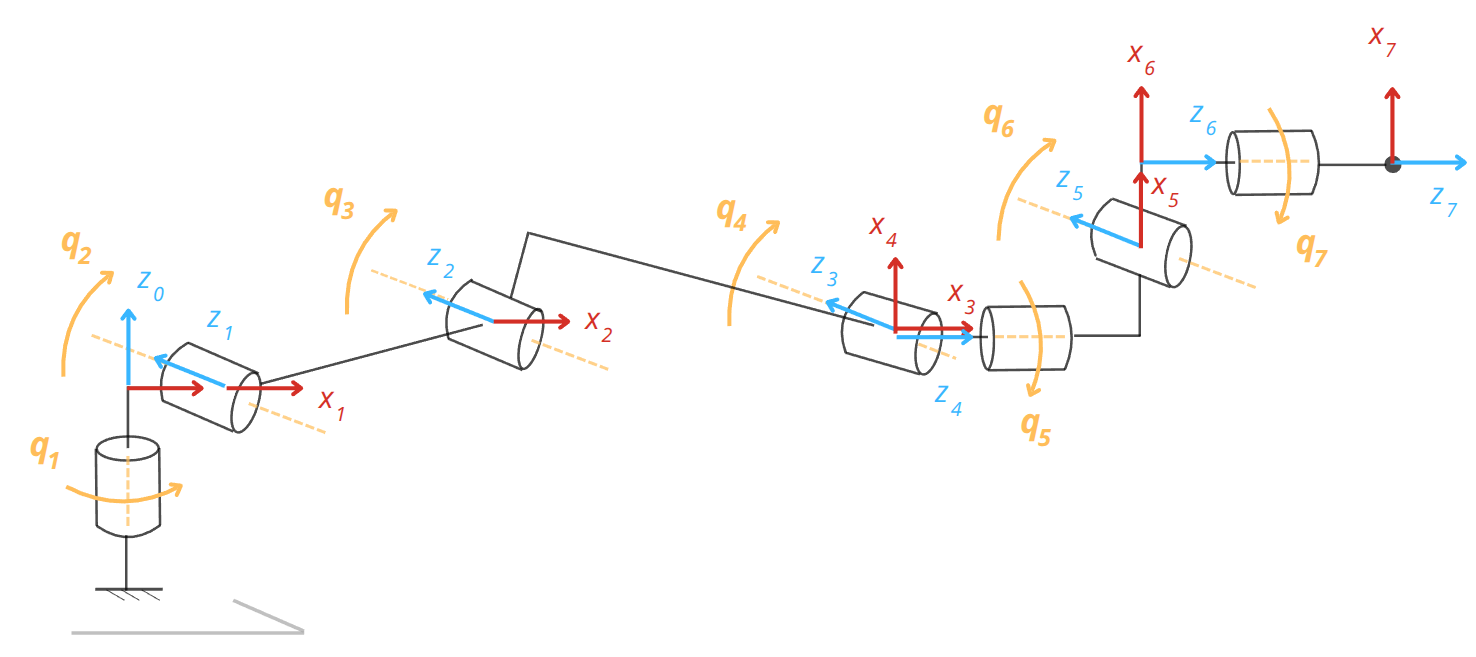
\includegraphics[width=0.8\textwidth]{Images/img_ch4/limbero_grieel_DH.png}
    \caption{LIMBERO-GRIEEL links and joints scheme with DH convention}
    \label{fig:limbero_grieel_DH}
\end{figure}

The overall LIMBERO-GRIEEL robot, composed of 4 limbs (LF,LH,RH,RF) with the structure described above, attached to a base, is reported in Fig.\ref{fig:LIMBERO_GRIEEL_robot} and Fig.\ref{fig:robot_LIMBERO_GRIEEL_GRIPPER_hw_front} below. 
\begin{figure}[H]
    \centering
    \subfloat[Gripper mode\label{fig:robot_LIMBERO_GRIEEL_GRIPPER_hw}]{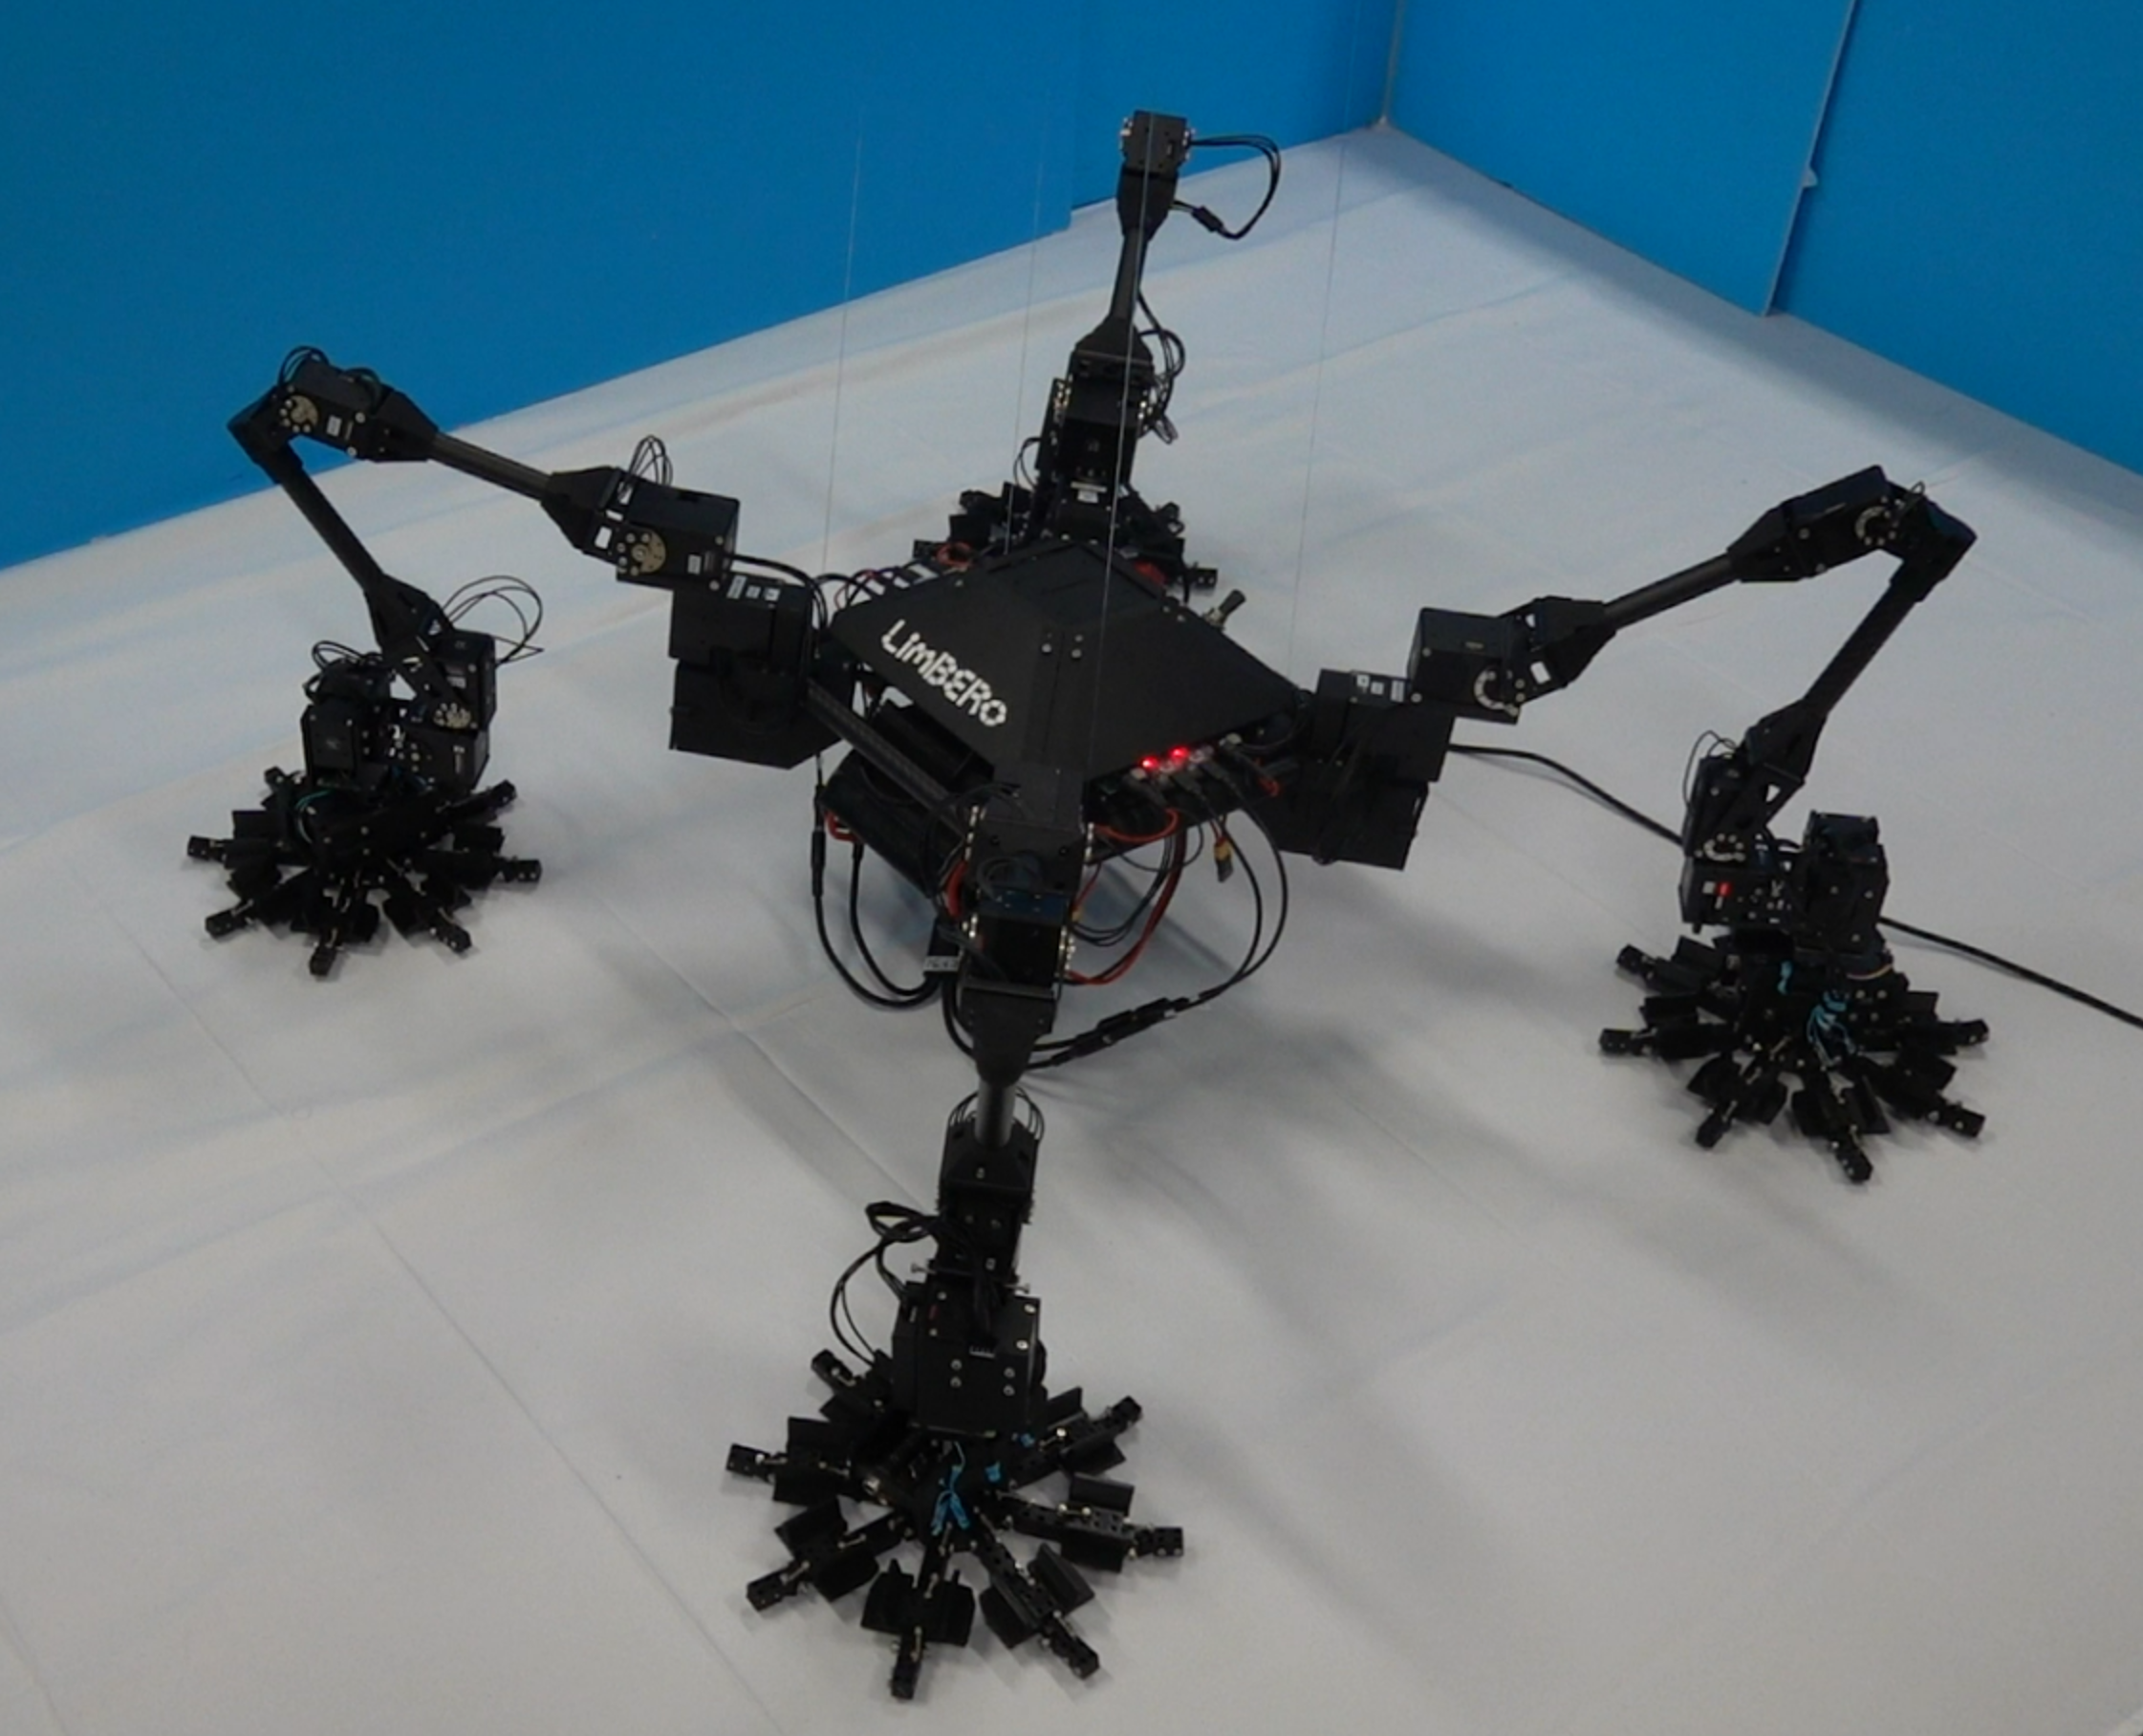
\includegraphics[width=0.35\textwidth]{Images/img_ch4/robot_LIMBERO_GRIEEL_GRIPPER_hw.png}} \quad 
    \subfloat[Wheel mode\label{fig:robot_LIMBERO_GRIEEL_WHEEL_hw}]{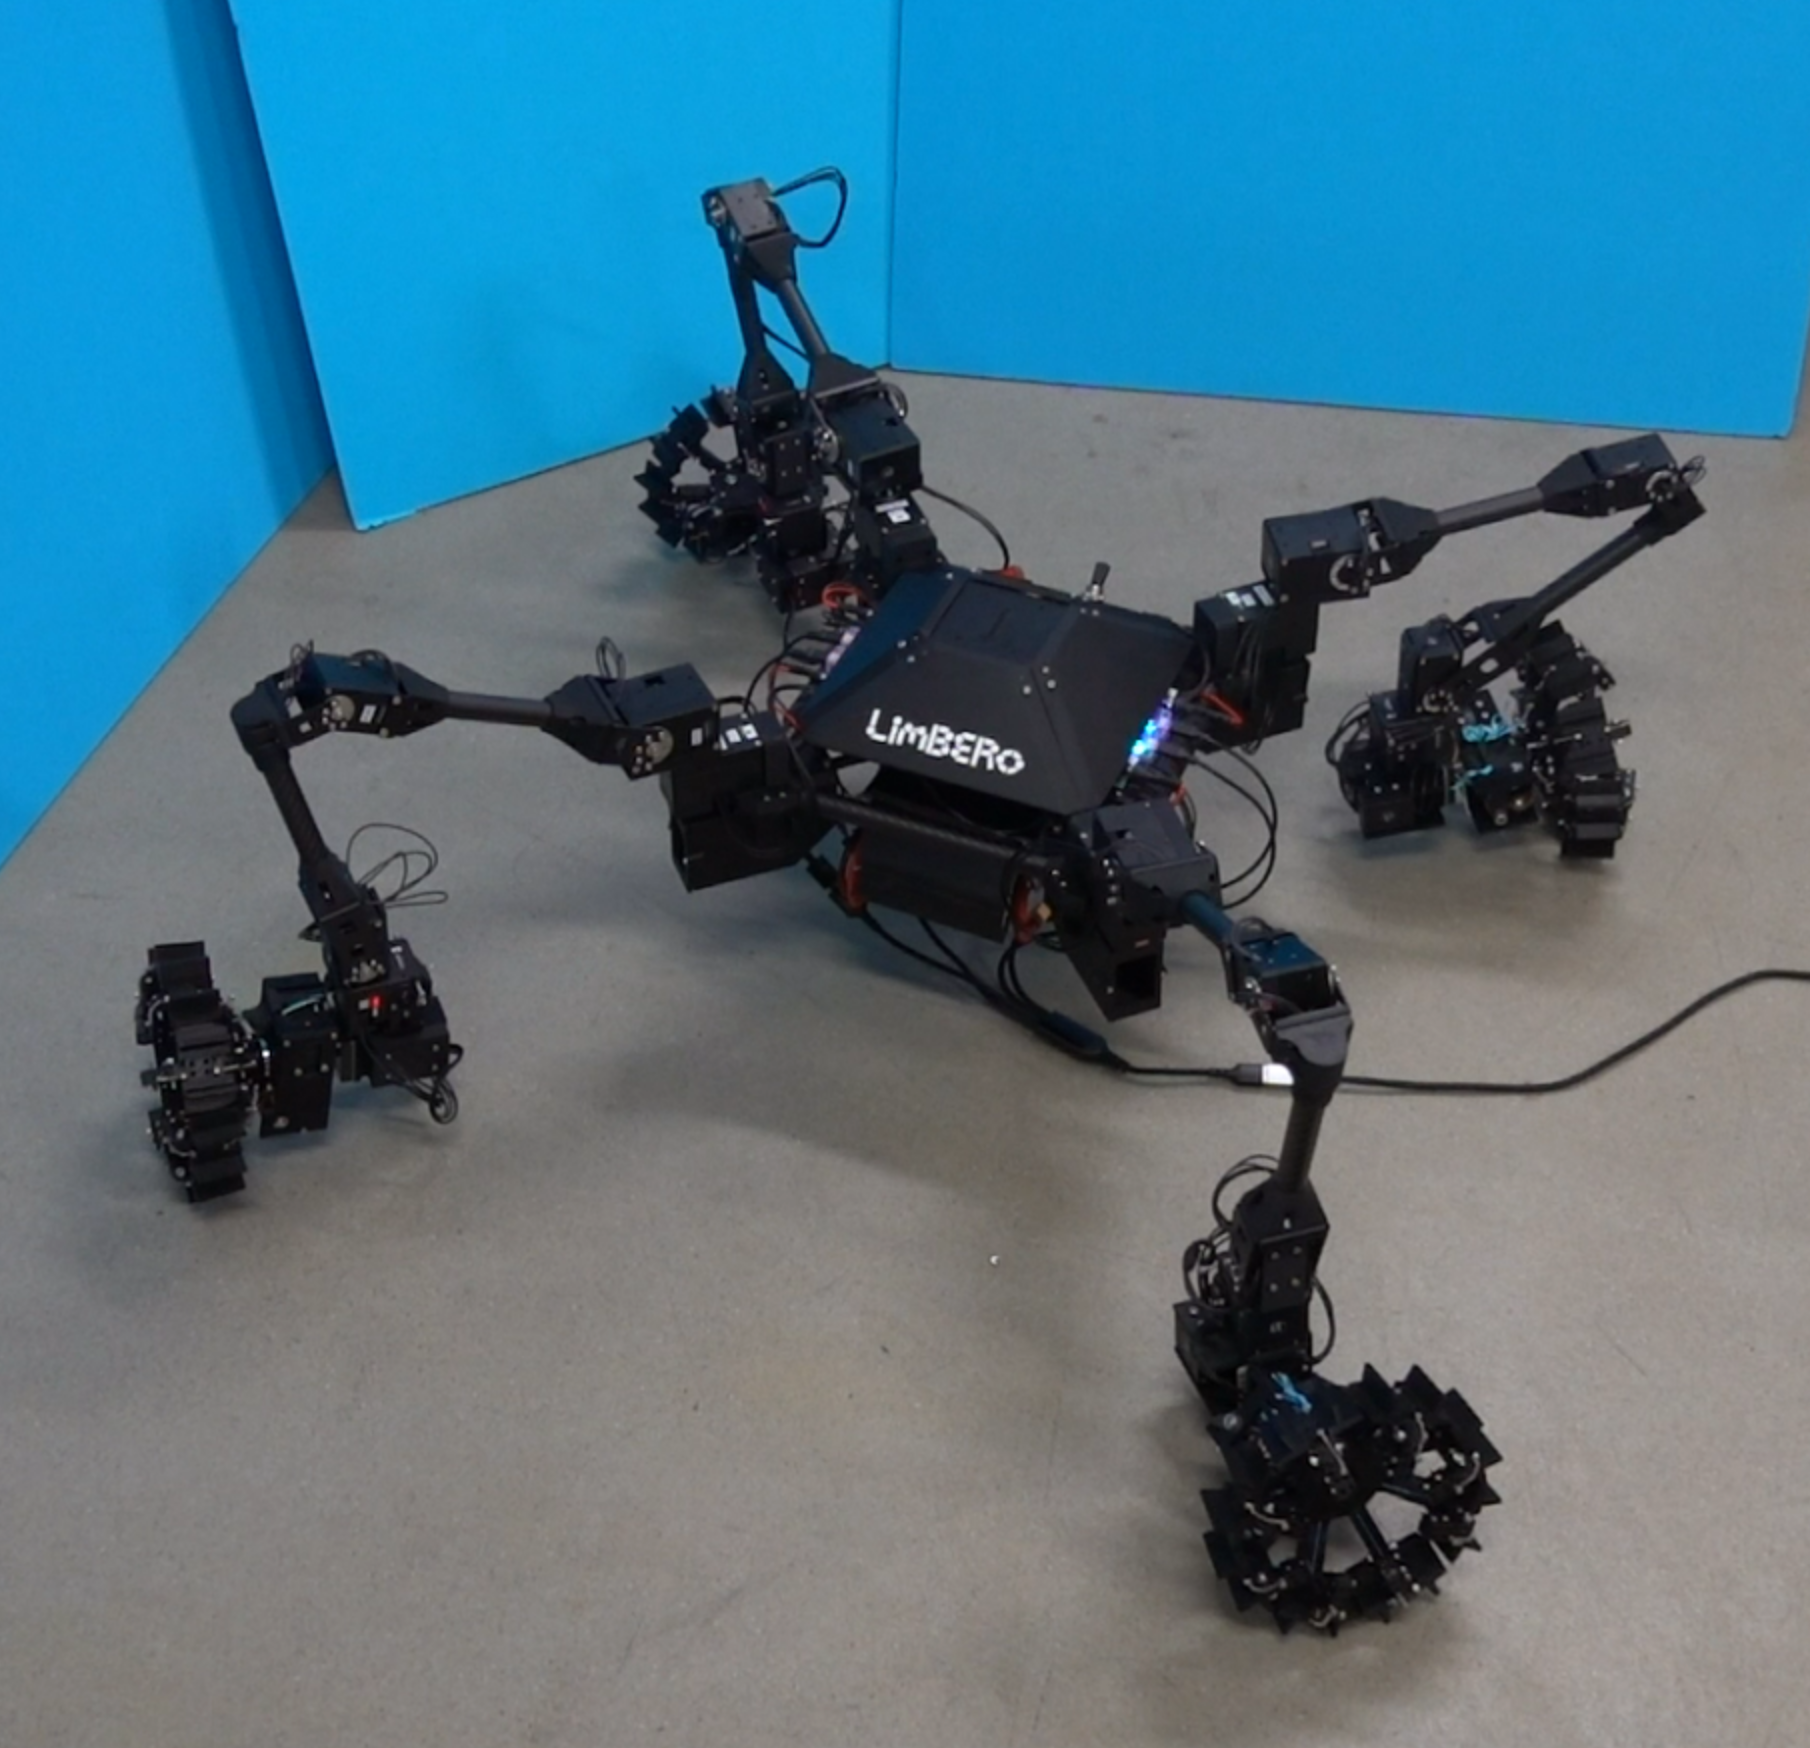
\includegraphics[width=0.3\textwidth]{Images/img_ch4/robot_LIMBERO_GRIEEL_WHEEL_hw.png}} 
    \caption[LIMBERO-GRIEEL robot]{LIMBERO-GRIEEL robot in wheel and gripper mode}
    \label{fig:LIMBERO_GRIEEL_robot}
\end{figure}

\begin{figure}[H]
    \centering
    \subfloat[Gripper mode front view \label{fig:robot_LIMBERO_GRIEEL_GRIPPER_hw_front}]{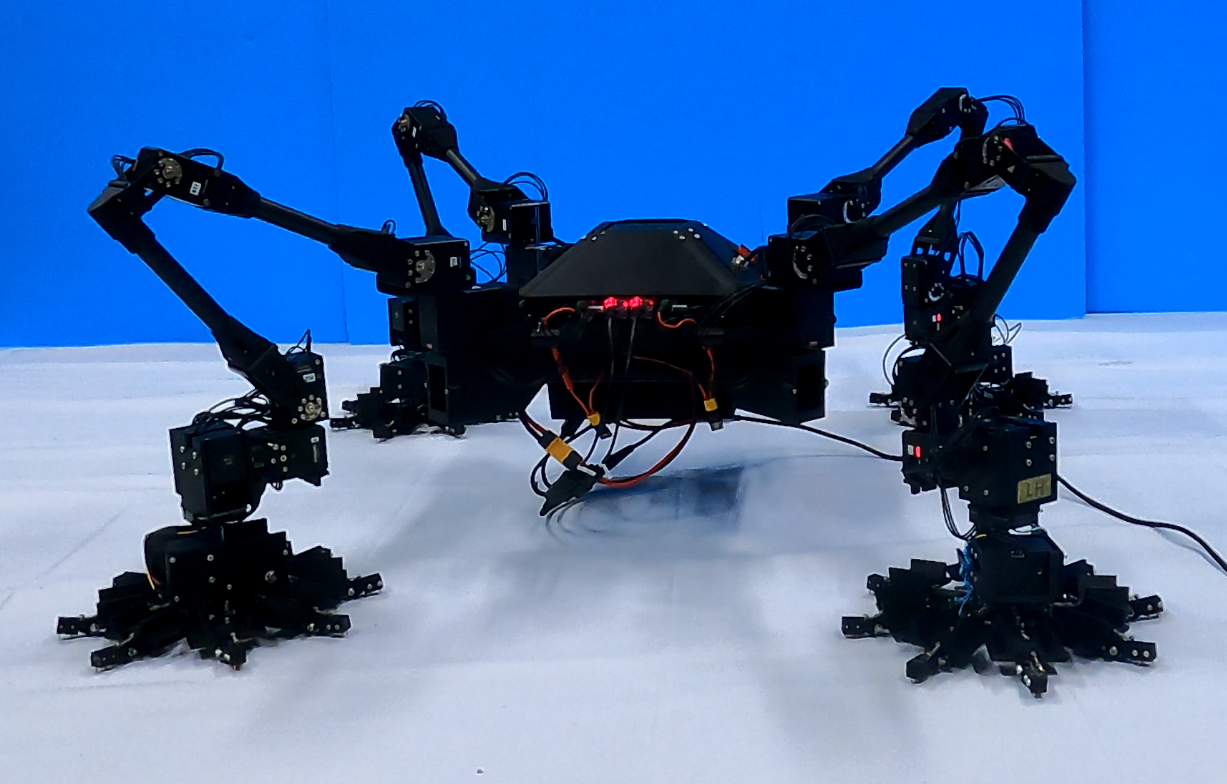
\includegraphics[width=0.35\textwidth]{Images/img_ch4/GripperMode_Front.png}} \quad 
    \subfloat[Wheel mode front view\label{fig:robot_LIMBERO_GRIEEL_WHEEL_hw_front}]{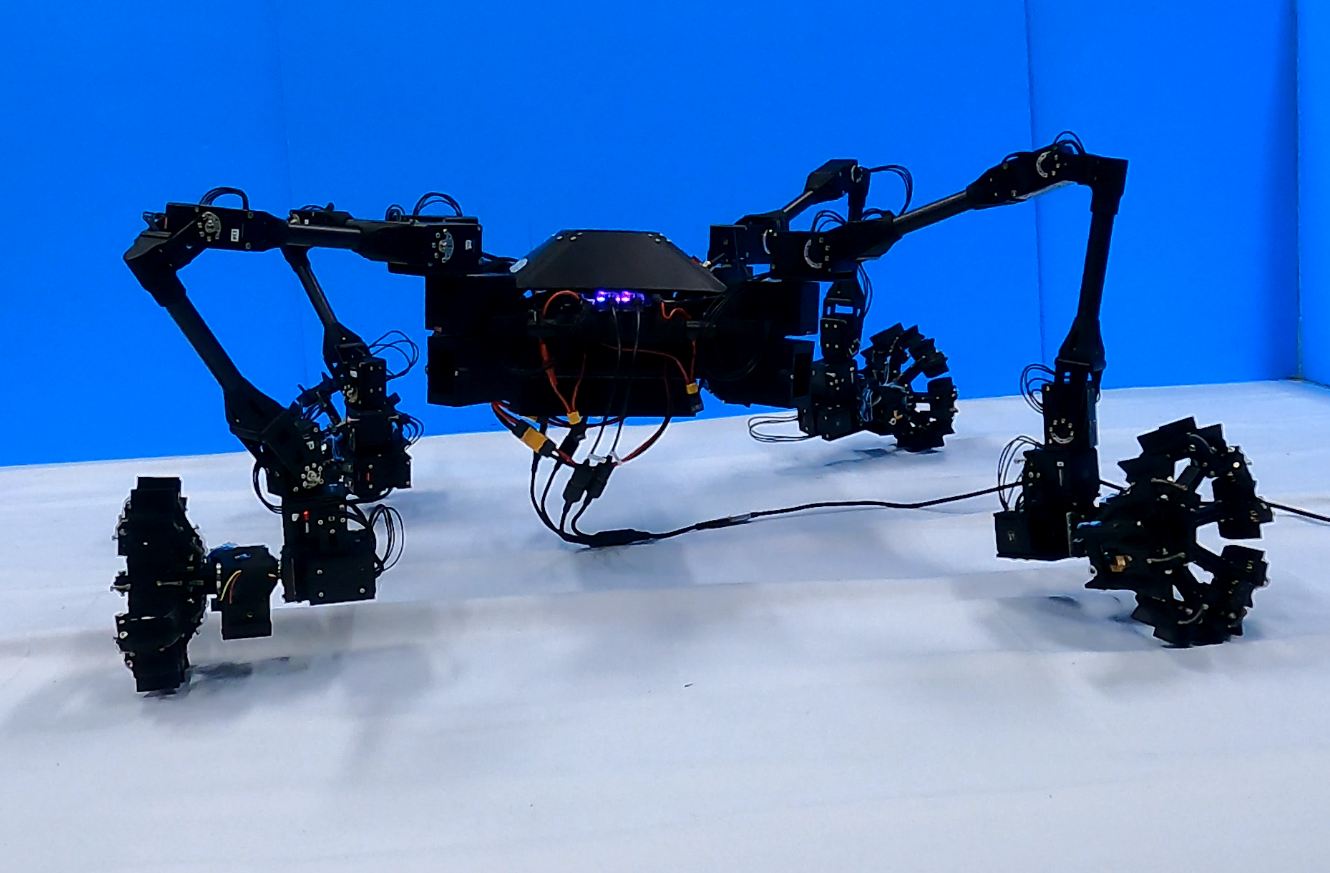
\includegraphics[width=0.35\textwidth]{Images/img_ch4/WheelMode_Front.png}} 

    \caption[LIMBERO-GRIEEL robot in wheel and gripper mode]{LIMBERO-GRIEEL robot in wheel and gripper mode}
    \label{fig:LIMBERO_GRIEEL_robot_front}
\end{figure}


This description of the limbs' joints and links neglects the DOFs used by the gripper-wheel mechanism for transformation, now considered as a single rigid body.
Next, the process of the transformation is briefly described, providing a complete model useful for simulation. 

\subsection{Gripper-Wheel Transformation}
\label{sec:gripper_wheel}

The final mechanism assembled and patented by M.Uda \cite{GrieelUda}\cite{GrieelUda} comes from the following design requirements:
\begin{enumerate}
    \setlength\itemsep{-0.7em} 
    \item Ability to switch between gripper and wheel at will.
    \item Ability to maintain sufficient grip on uneven terrain and steep slopes. 
    \item High driving performance. 
\end{enumerate}

The system is composed of eight fingers in an equally spaced radial disposition around a central "hand", each finger has four links, interconnected by passive rotational joints with springs and an internal tether. Each finger's tip has for claws for gripping capabilities, widely tested during prototyping.
As represented in Fig.\ref{fig:Gripper_Wheel}, the mechanism is in gripper mode when all fingers are opened, and in wheel mode when closed. The Transformation from gripper to wheel (G2W) is achieved by pulling all the tethers, which are connected to a single servo motor, with a locking function achieved using a worm gear. 
The opposite mode transformation (W2G) instead releases the tethers rotating the servo motor in the opposite direction and exploits the restoring force of the springs to open the fingers. A schematic view of the closing sequence for one finger is represented in Fig.\ref{fig:closing_finger}, while the real finger design and overall mechanism with the transforming servo motor is in Fig.\ref{fig:Gripper_Wheel_mechanism}.

The servo motor used to open and close the mechanism is not included in the joint space of the limb because it doesn't contribute to the positioning of the EE, but to the locomotion change. Considering a single finger, the palm is considered as part of the central hand link, denoting the links as {phalanx1, phalanx2, phalanx3}, and the passive joints as $\{H2P1,\; P12P2,\; P22P3\} = \{\theta_1, \theta_2, \theta_3\} $. The springs are chosen with a spring constant such that, the mimic behavior of the finger joints respects the following constraints:
\begin{equation}
    \label{eq:finger_contraint}
    \left\{
    \begin{aligned}
           \theta_2 = 2\cdot\theta_1  \\
            \theta_3 = 3\cdot\theta_1
    \end{aligned}
    \right.
\end{equation}
With those constraints, in closing finger configuration 
$\theta_1 = \frac{\pi}{6}\;,  \theta_2 = \frac{\pi}{3} \;, \theta_3 = \frac{\pi}{2}$, exactly as represented in Fig.\ref{fig:closing_finger}, and the connection of the eight tethers in the central mechanism guarantee the coordination of all fingers motion (imposing the additional constraint that each finger $\theta_1$ is equal. 

\begin{figure}[H]
    \centering
    \subfloat[\label{fig:closing_finger1}]{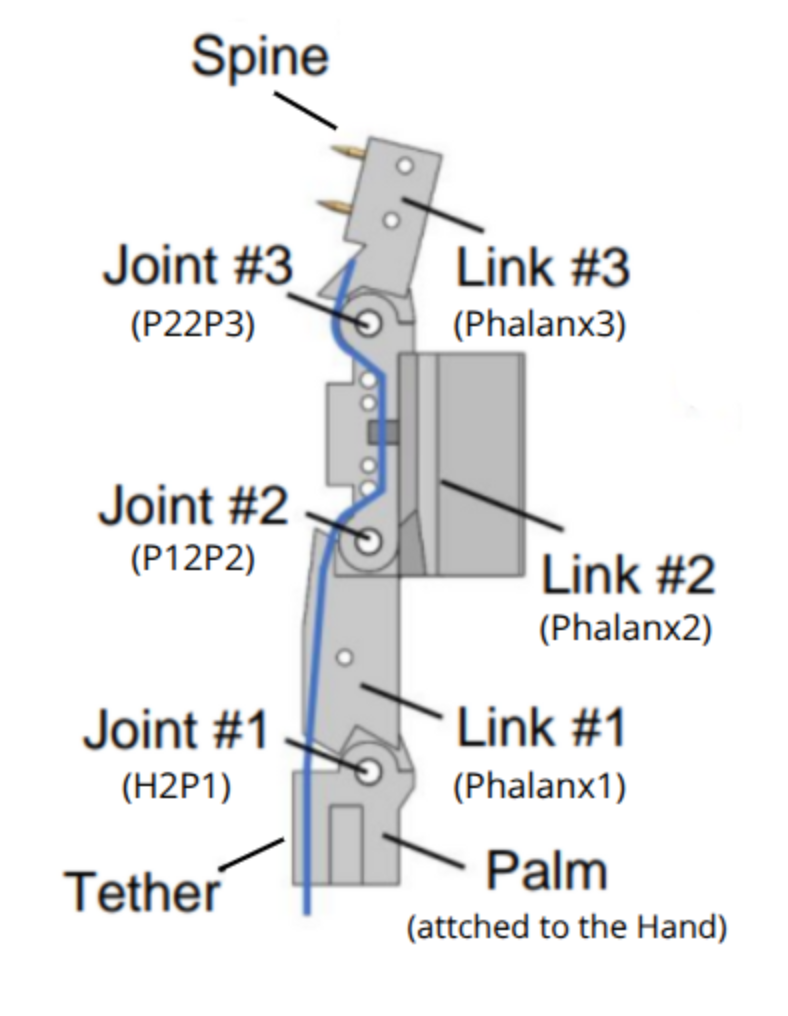
\includegraphics[scale=0.15]{Images/img_ch4/closing_finger1.png}}
    \subfloat[\label{fig:closing_finger2}]{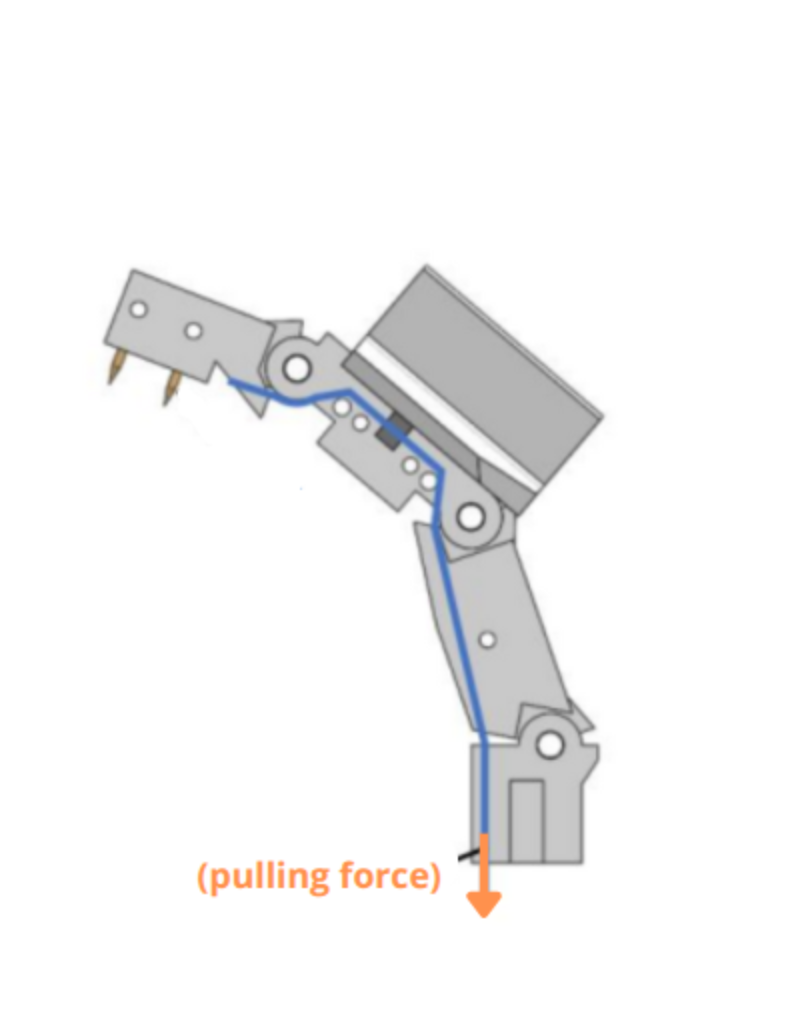
\includegraphics[scale=0.15]{Images/img_ch4/closing_finger2.png}}
    \subfloat[\label{fig:closing_finger3}]{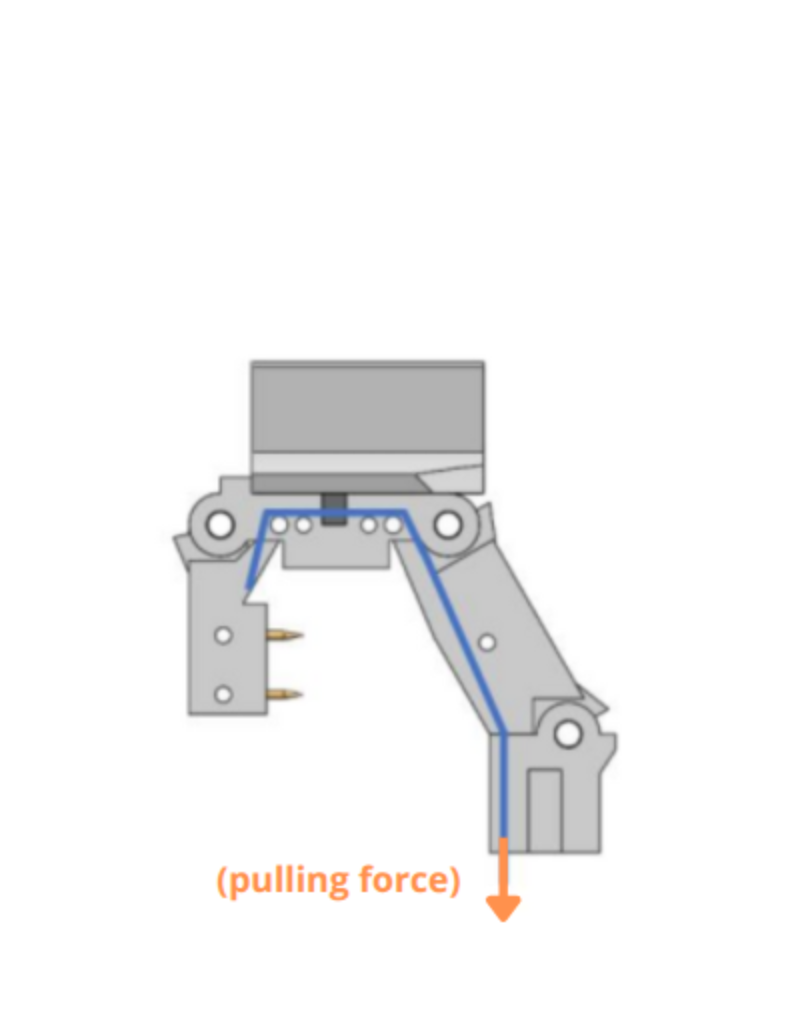
\includegraphics[scale=0.15]{Images/img_ch4/closing_finger3.png}}
    \caption[gripper-wheel mechanism G2W finger sequence]{\cite{GRIEELUdaThesis} representation of single finger closing sequence for G2W transformation: (a) open (Gripper),(b) in transition, (c) closed state (Wheel)}
    \label{fig:closing_finger}
\end{figure}
    

\begin{figure}[H]
    \centering
    \subfloat{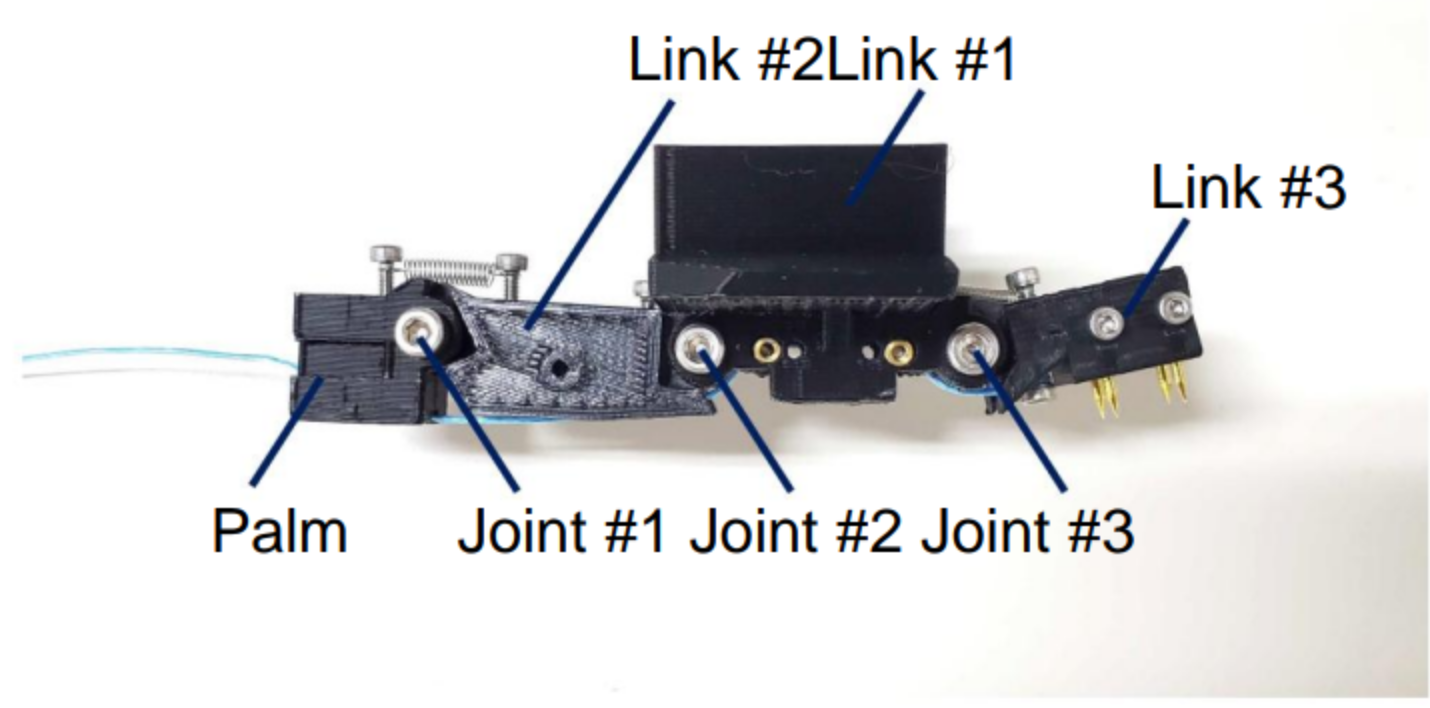
\includegraphics[width=0.4\textwidth]{Images/img_ch4/Gripper_Wheel_mechanism_finger.png}}\quad
    \subfloat{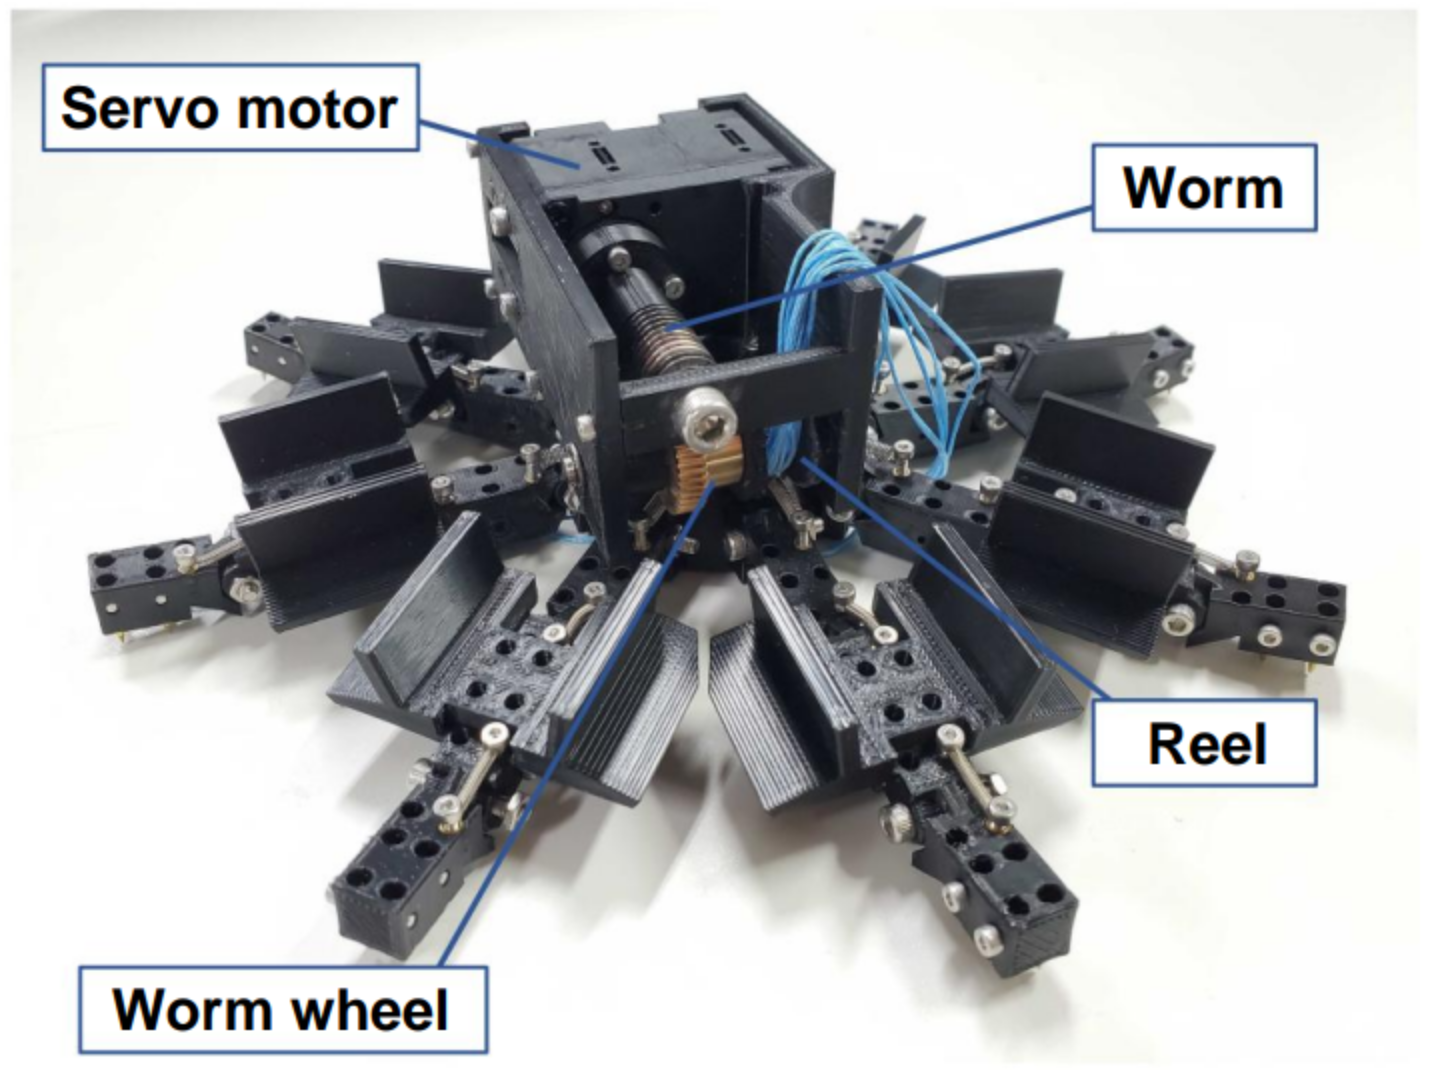
\includegraphics[width=0.4\textwidth]{Images/img_ch4/Gripper_Wheel_mechanism_all.png}}
    \caption[Single Finger and overall gripper-wheel mechanism]{\cite{GRIEELUdaThesis} Finger and overall gripper-wheel mechanism}
    \label{fig:Gripper_Wheel_mechanism}
\end{figure}

Expanding the notation to consider all the fingers of one mechanism,\\ the prefix $j\_Fk\_<link>$ is used to represent $j^{th}$ limb $k^{th}$ finger, and Fig.\ref{fig:TFTree_FINGERS} describes the mechanism links and passive joints interconnection tree, with the mimic constraint defined above. 

\begin{figure}[H]
    \centering
    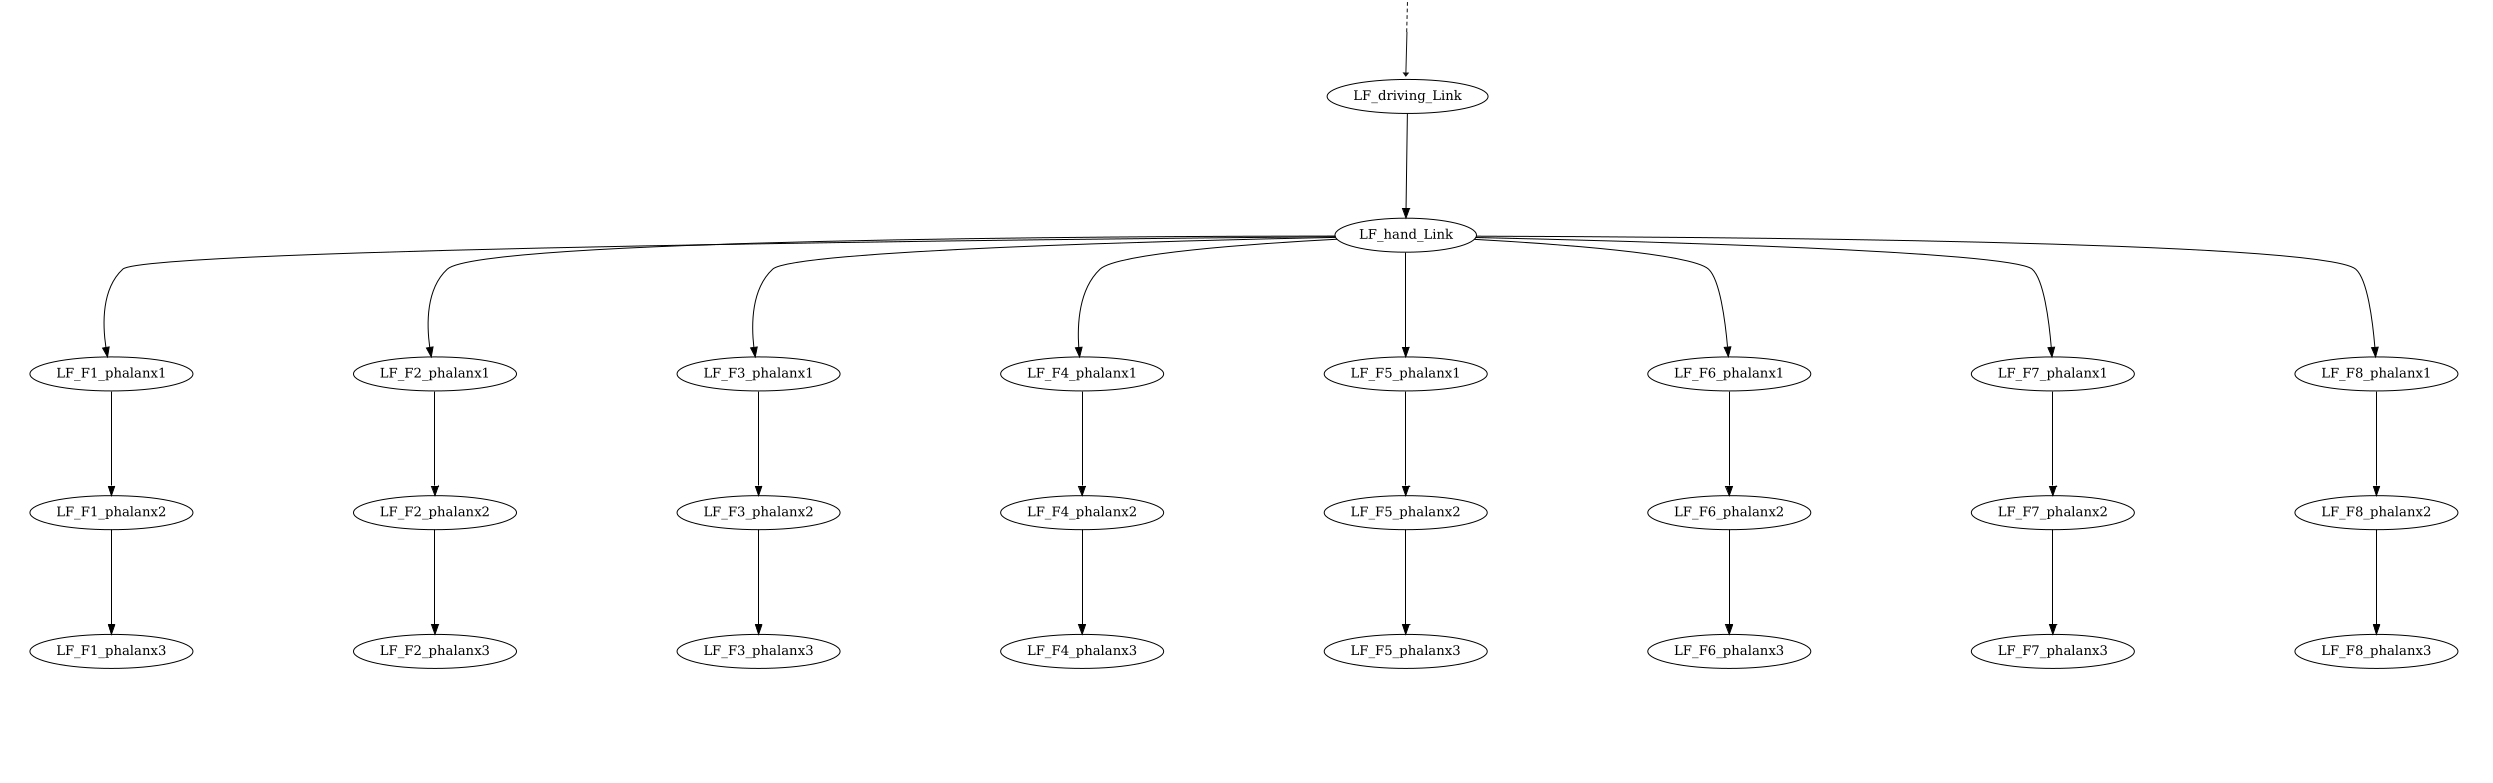
\includegraphics[width=1.0\textwidth]{Images/img_ch4/TFTree_FINGERS.png}
    \caption{Links structure of LF GRIEEL module joints, it is the expansion of LF\_gripper/wheel\_Link of Fig.\ref{fig:TFTree_NOFINGERS}, with a complete links-joints structure of the module, the same holds for LH,RH, and RF.}
    \label{fig:TFTree_FINGERS}
\end{figure}

During the design of GRIEEL, also the mounting mechanism has been developed with the specific purpose of transitioning efficiently between the two locomotion modes and driving the wheels.\\ 
The configuration transition and wheel rotation are achieved with the DOFs previously described, wristH and wristV joints for the first task, while driving joint for the second. Fig.\ref{fig:GRIEEL_GRIPPER_WHEEL} represents the standard configuration in the two modes:
\begin{itemize}
    \setlength\itemsep{-0.5em} 
    \item \textbf{Gripper mode}: $wristH = 0 \;, \; wristV = 0$
    \item \textbf{Wheel mode}: $wristH = \pi \;, \; wristV = \frac{\pi}{2}$
\end{itemize}

The W2G mode transition sequence is represented below in Fig.\ref{fig:GRIEEL_mode_transition}.
\begin{figure}[H]
    \centering
    \subfloat[Wheel mode \\($wristH = \pi, wristV = \pi/2$)\label{fig:W2G_1}]{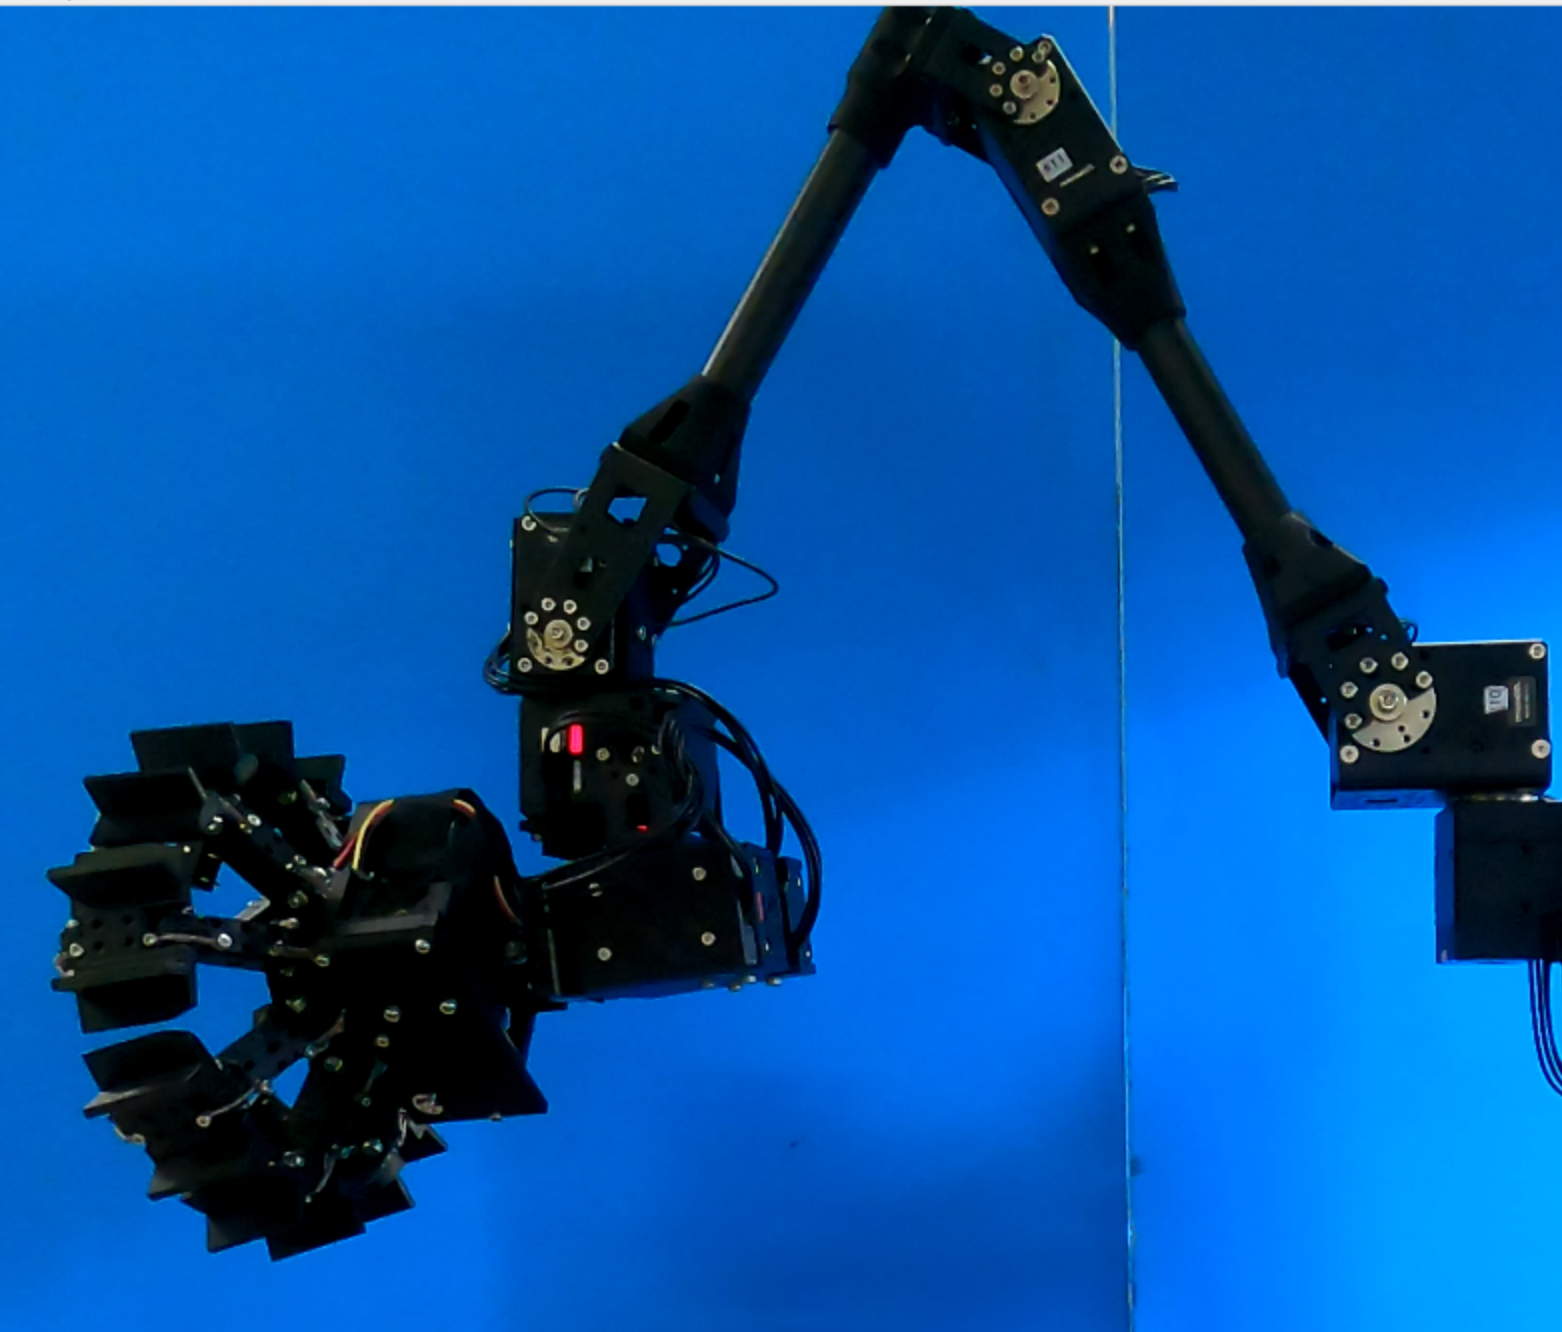
\includegraphics[width=0.3\textwidth]{Images/img_ch4/W2G_1.png}} \quad 
    \subfloat[Start transition of wrist\label{fig:W2G_2}]{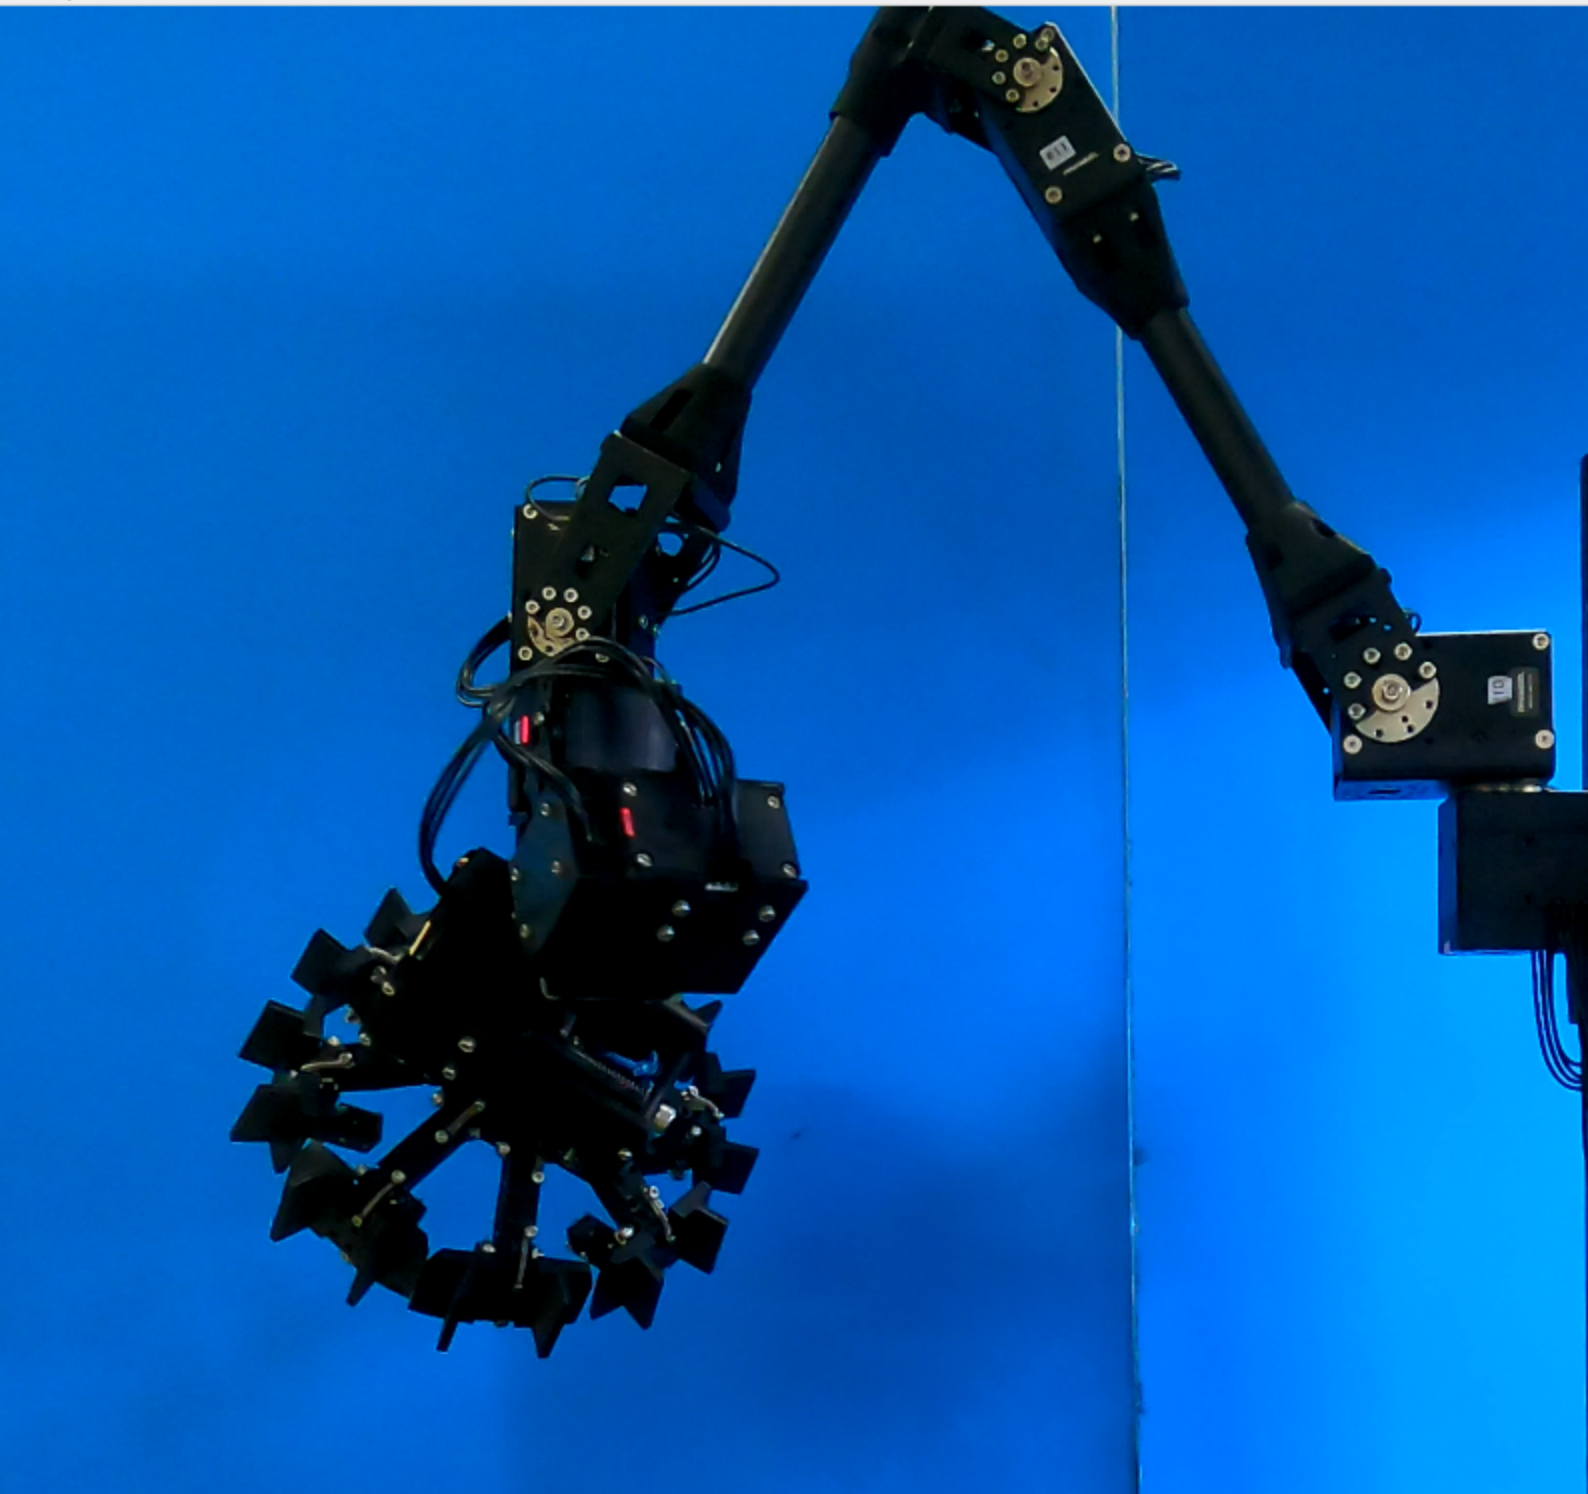
\includegraphics[width=0.3\textwidth]{Images/img_ch4/W2G_2.png}} \quad
    \subfloat[Reached wrist config.\label{fig:W2G_3}]{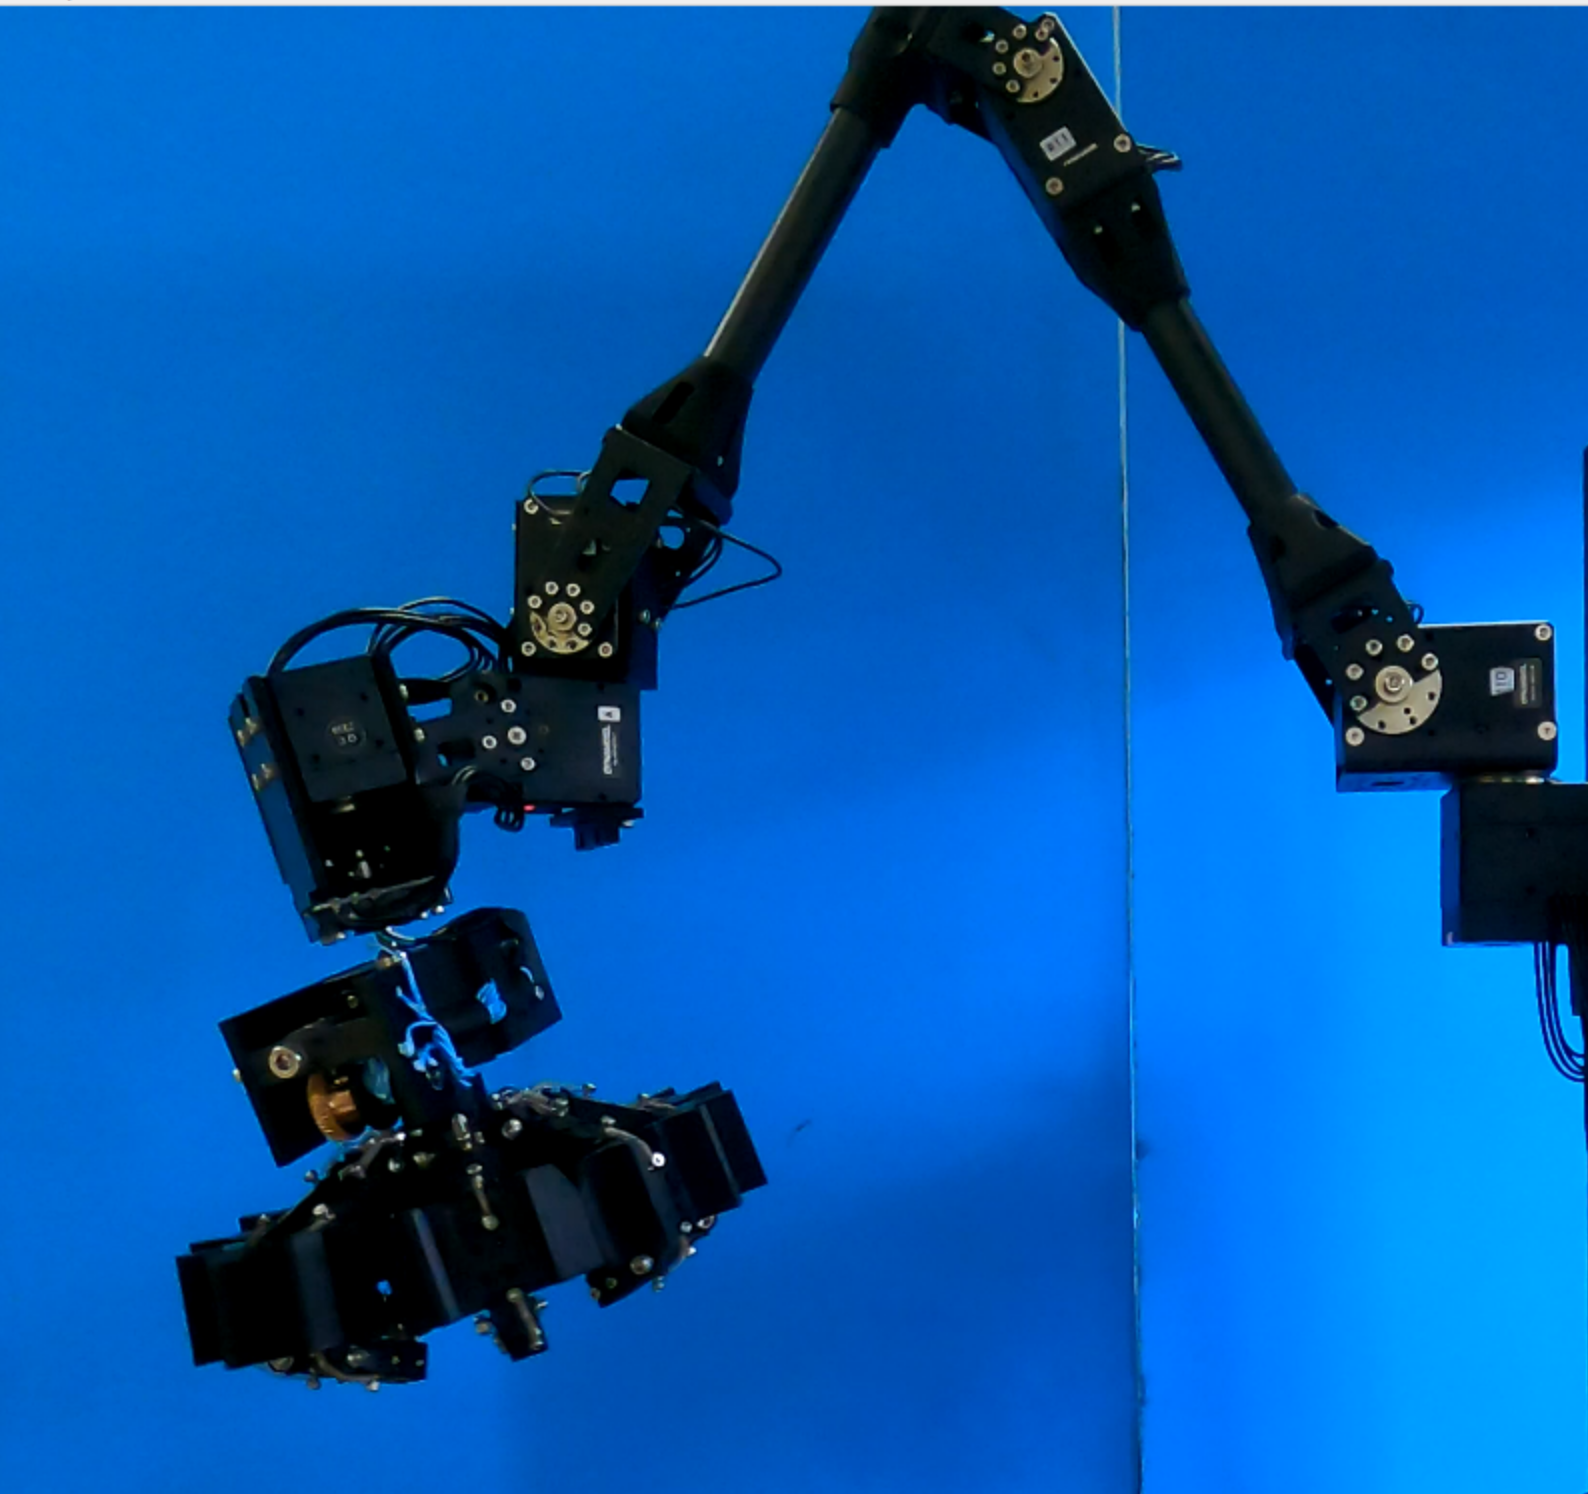
\includegraphics[width=0.3\textwidth]{Images/img_ch4/W2G_3.png}}   \quad
    \\
    \subfloat[Releasing the tethers\label{fig:W2G_4}]{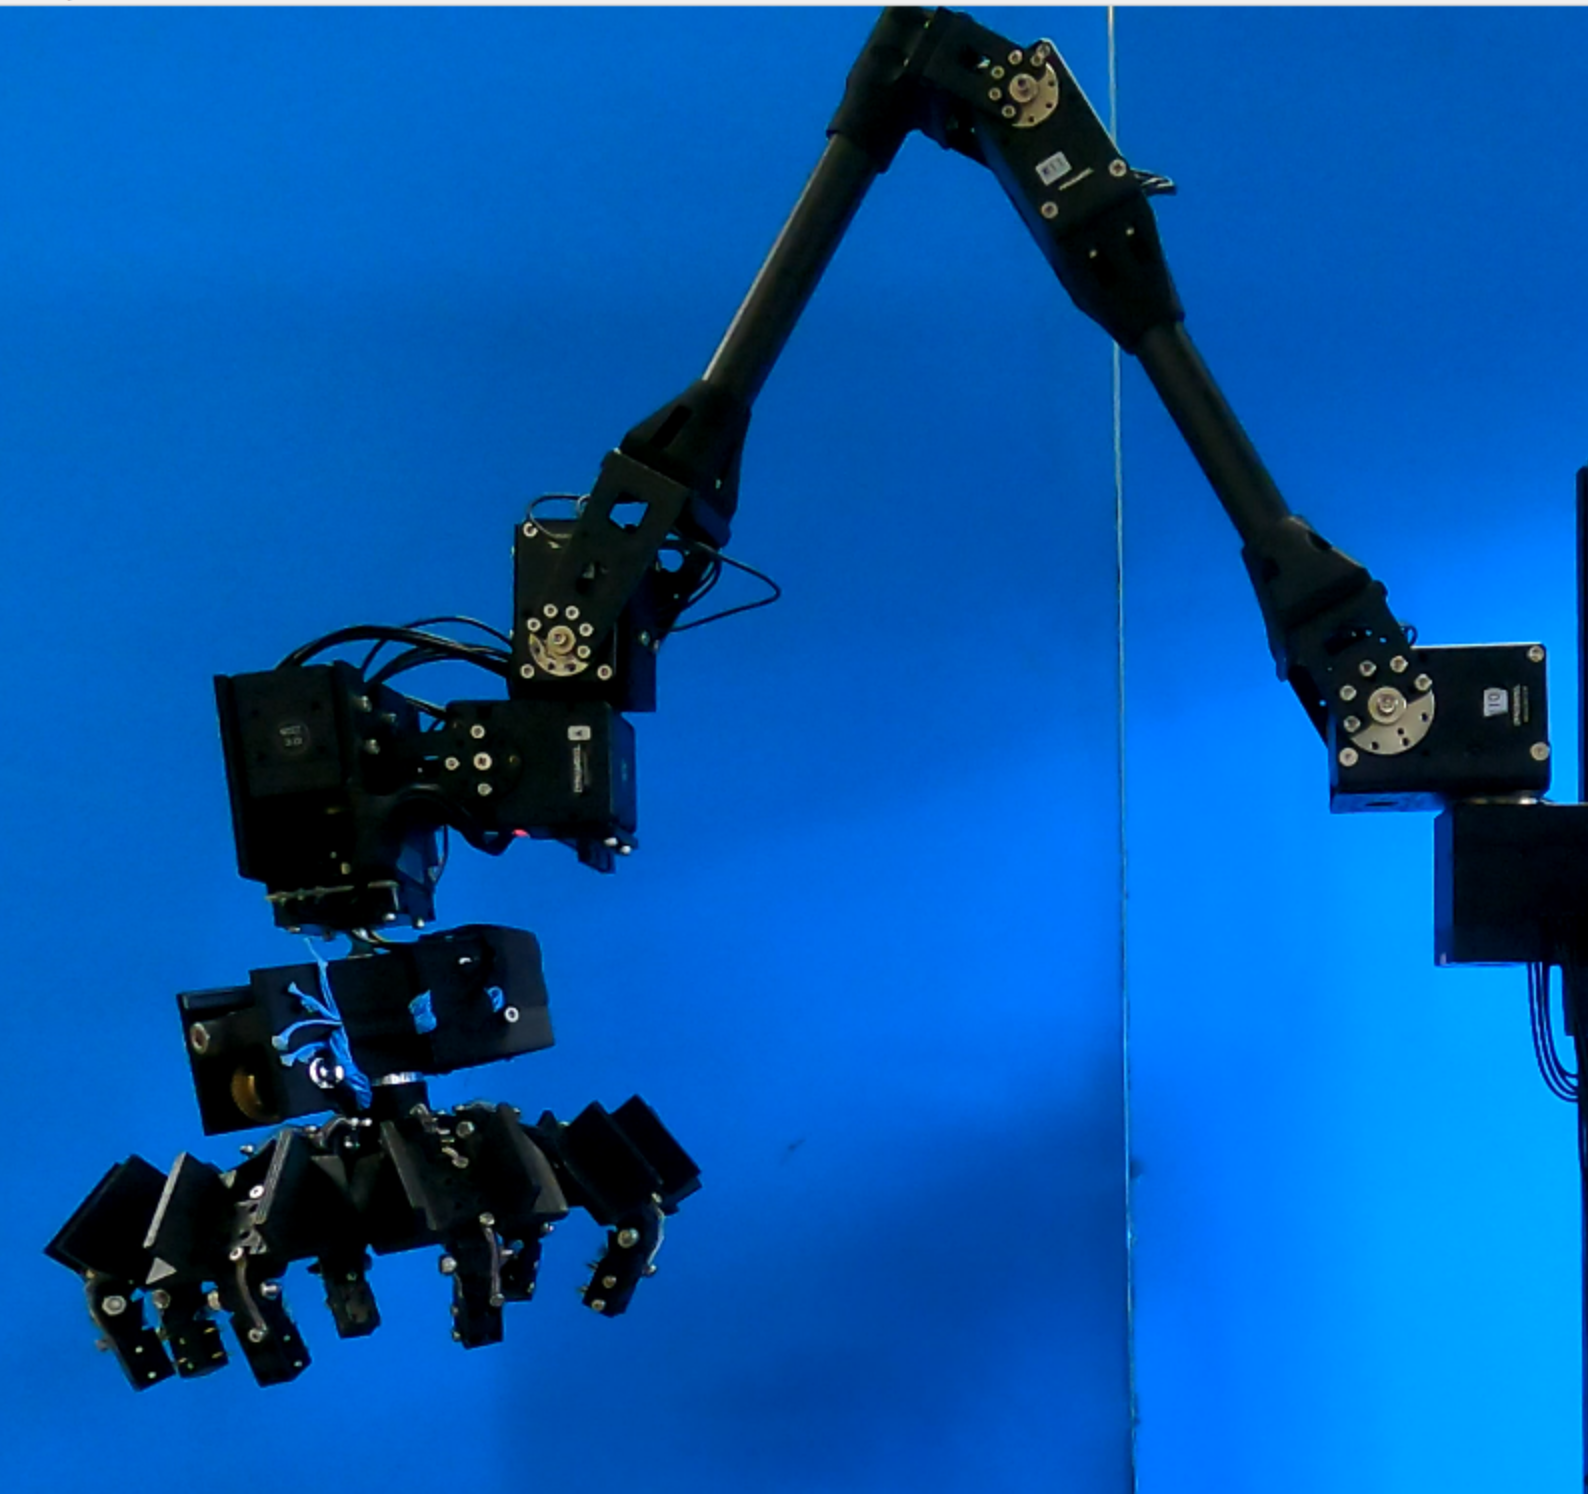
\includegraphics[width=0.3\textwidth]{Images/img_ch4/W2G_4.png}}\quad
    \subfloat[Gripper mode\\($wristH =0, wristV = 0$)\label{fig:W2G_5}]{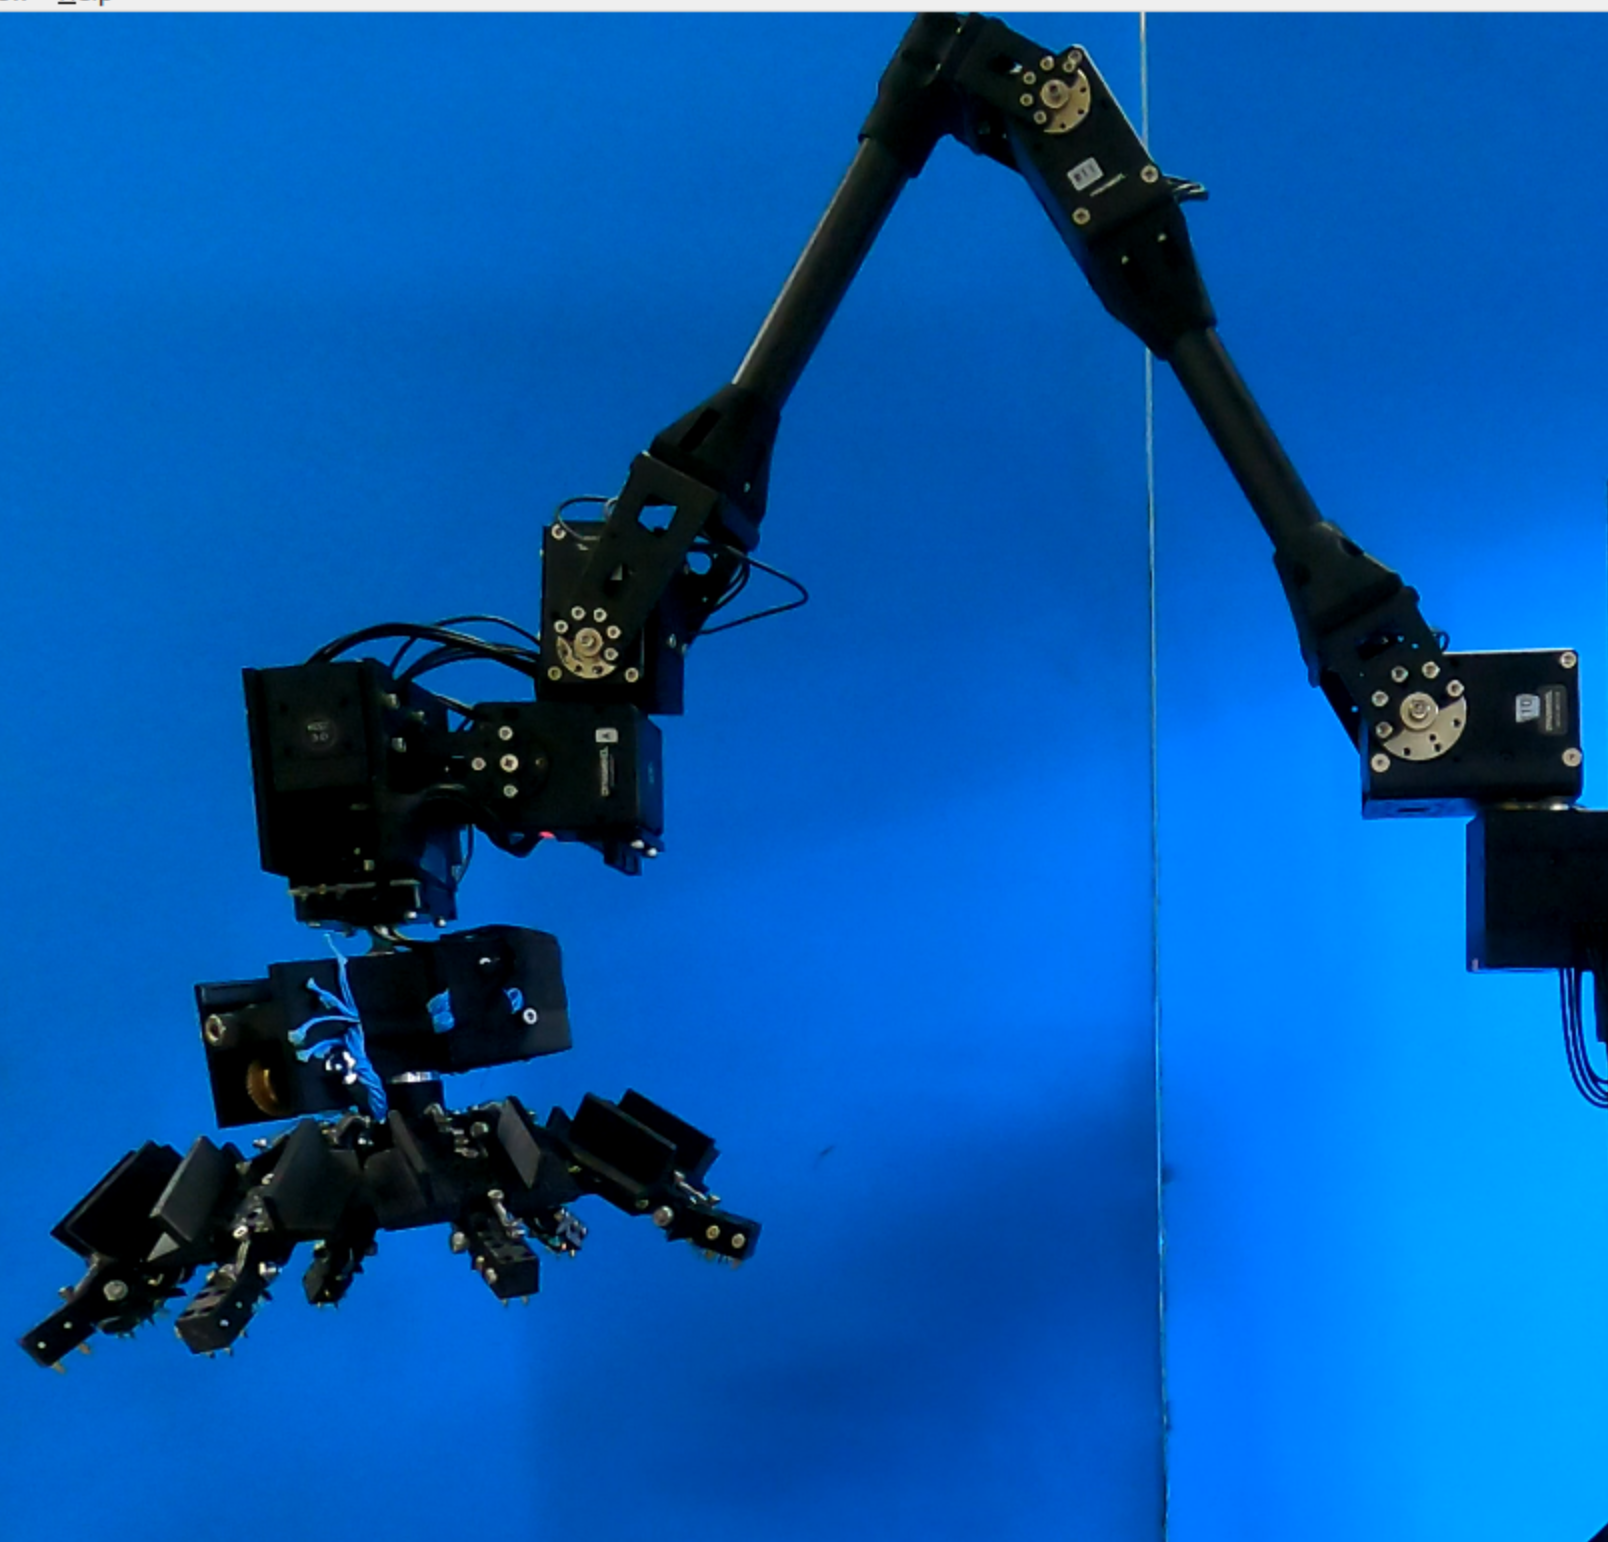
\includegraphics[width=0.3\textwidth]{Images/img_ch4/W2G_5.png}}
    
    \caption[W2G transition sequence]{W2G transition sequence}
    \label{fig:GRIEEL_mode_transition}
\end{figure}

\subsection{Kinematics}
\label{sec:kin}

FK and IK computations, required for motion control of the end-effector, are computed analytically from geometric considerations. The explicit expression is not reported here because not relevant to this research, instead, it is important to clarify the approximation used in those computations. 

As noticed in Chapter \ref{ch:chapter_two}, IK is complex to derive, and the 3 DOFs of GRIEEL (which are not in spherical wrist configuration\cite{Siciliano})  add further complexity. For this reason, the previously developed kinematics computations for LIMBERO's limb are used in the motion controller. This approach is possible if the overall GRIEEL mechanism as a whole is considered as the limb end effector. 

In using this kinematic approximation, the real positioned frame is the one on the link attached to LIMBERO's limb-end, controlled in position and pitch from the previous IK, using the first 4 DOFs. This means that GRIEEL's DOFs are used to control the W2G and G2W transformations and maintained on the desired mode configuration otherwise.  
The details of the implementation of this as part of the kinematics computation in the motion control software are not discussed here.

This choice can be justified by two reasons: 
\begin{enumerate}
   \setlength\itemsep{-0.7em} 
    \item After the first test with the original kinematics, it was noticed that for the tasks involved, there was no need to update the kinematic. 
    limb and base tasks in fact were completed correctly, and mode transition was possible with a decoupled control of wrist joints. 
    \item The design of GRIEEL used in this research is the original prototype, but a new one is under development, as discussed in the last chapter \ref{ch:chapter_nine}. For this reason, rather than defining low-level kinematics computations, more emphasis has been placed on defining high-level algorithms, easy to integrate with the novel system. 
\end{enumerate}

In conclusion, the limb is controlled with the first 4 DOFs in position and pitch angle (which correspond to the sum of $q2+q3+q4$), and mode transition or driving is achieved with a decoupled control of the additional 3 DOFs. However, some tests considering the overall limb structure with its 7 DOFs are conducted with the DH kinematic model defined in MATLAB.

\subsection{Driving, Walking (and Climbing)\\ Locomotion Configurations}
\label{sec:locomotion_configurations}

The potential locomotion capabilities of LIMBERO-GRIEEL are enforced by its redundant limbs, which allow for grasping almost unreachable points during walking or climbing. Even in driving mode, advanced limb configurations could be exploited to achieve better wheeled traversability than conventional rovers. 

the system is not yet ready for such functionality, and now the two main mechanical configurations that have been tested both in simulation and hardware experiments are described. 

\textbf{Walking/Climbing Mode}

The gait scheduler for LIMBERO-GRIEEL is under development, and advanced algorithms for foothold planning will be integrated \cite{LIMBEROTakadaThesis}. 
As discussed, the default walking/climbing configuration uses an insect leg configuration \cite{KentaroUnoPhD}\cite{Todd}, which is represented in Fig.\ref{fig:limbero_walking}.  

\begin{figure}[H]
    \centering
    \subfloat{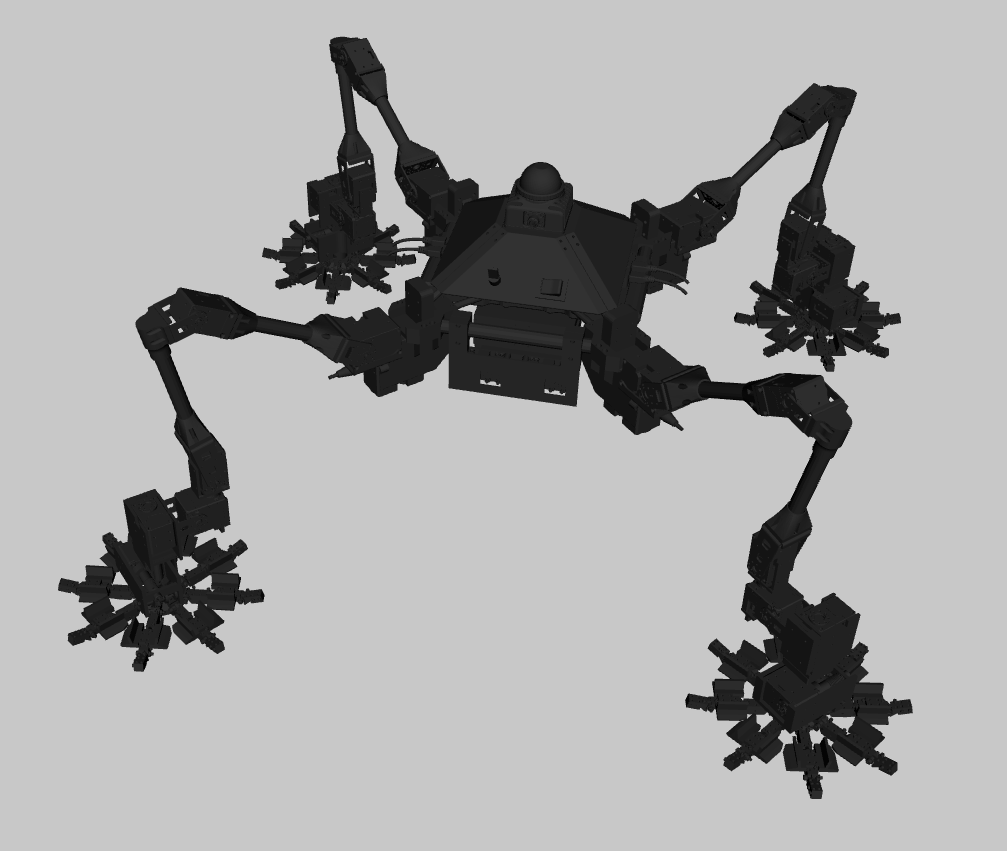
\includegraphics[width=0.45\textwidth]{Images/img_ch4/LIMBERO_GRIEEL_walking.png}}\quad
    \subfloat{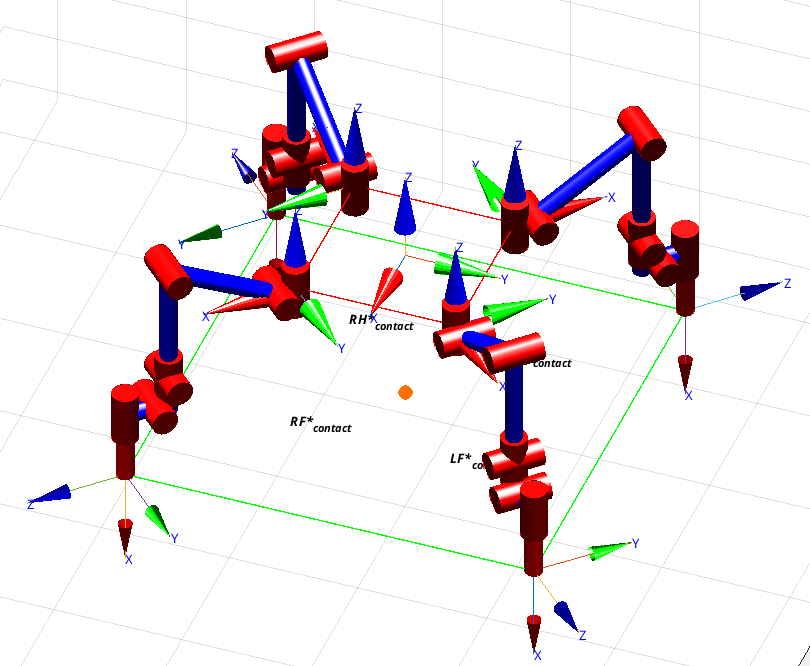
\includegraphics[width=0.45\textwidth]{Images/img_ch4/LIMBERO_GRIEEL_walking_model.png}}
    \caption[LIMBERO-GRIEEL model in wolking/climbing configuration]{LIMBERO-GRIEEL model in wolking/climbing configuration}
    \label{fig:limbero_walking}
\end{figure}

\textbf{Driving Mode}

In principle, $wristH$ joint can be used to perform omnidirectional drive capabilities\cite{Siciliano}. Even if at the current state, driving locomotion has not been designed, wheel rotation commands have been integrated into the limb control software during this research. With this command, it is possible to test the controller's performance when rotating the wheels and perform simple driving tests in simulation. 

To test wheeled locomotion, a simple driving limbs configuration has been considered with wheels facing forward, parallel to the base frame x direction. This configuration is represented in Fig.\ref{fig:limbero_driving} below.
\begin{figure}[H]
    \centering
    \subfloat{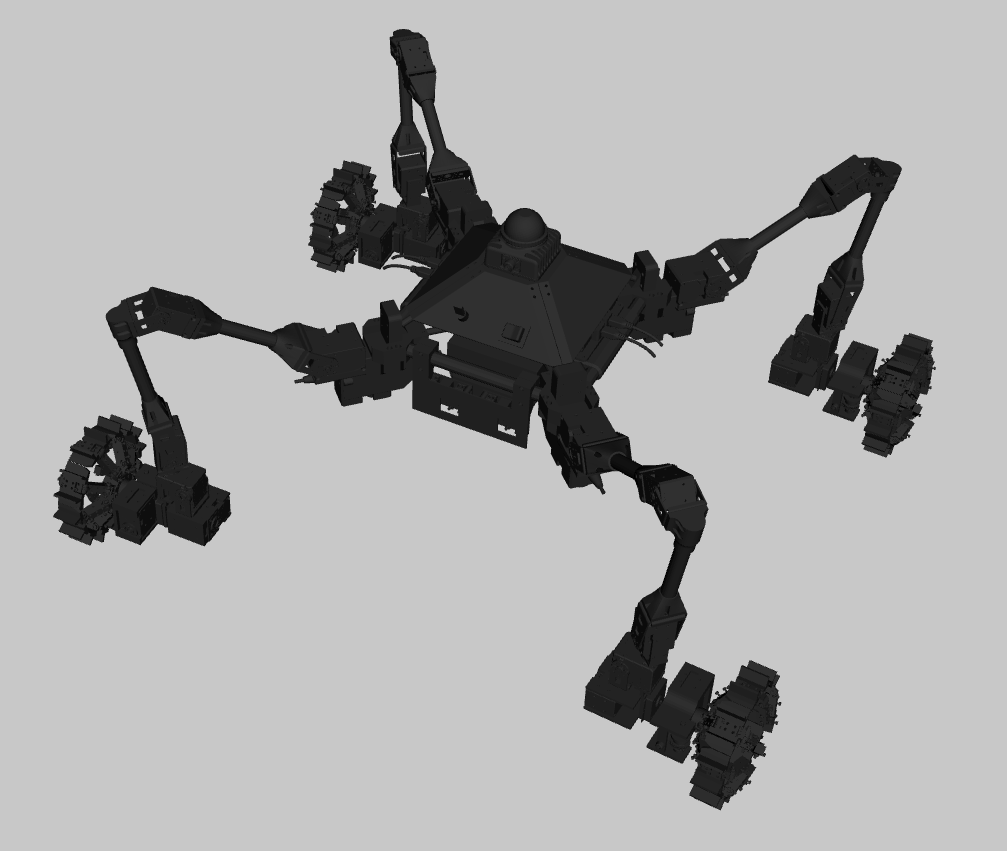
\includegraphics[width=0.45\textwidth]{Images/img_ch4/LIMBERO_GRIEEL_driving.png}}\quad
    \subfloat{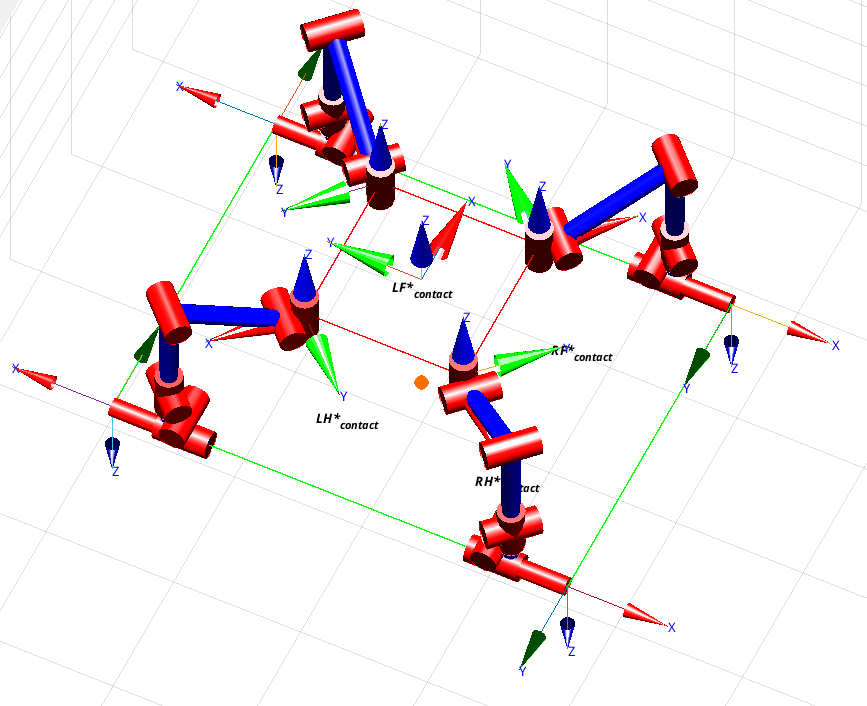
\includegraphics[width=0.45\textwidth]{Images/img_ch4/LIMBERO_GRIEELdriving_model.png}}
    \caption[LIMBERO-GRIEEL model in driving configuration]{LIMBERO-GRIEEL model in driving configuration}
    \label{fig:limbero_driving}
\end{figure}

In this standard driving configuration, it is possible to drive LIMBERO-GRIEEL forward/backward, using the limbs as rigid wheel attachments.

As is evidenced by much research on wheel-on-leg rovers, integrating active limb reconfigurations can equalize traction forces on wheels, ensuring narrow passageways and clamber over obstacles\cite{MAMMOTH}\cite{WheelLeggedStabilityOPT}\cite{WheleedLeggedLUNAR}\cite{WheeledLeggedAMAZONFOREST}. This will be integrated in the final driving controller.

\subsection{Electronics}
\label{sec:electronics}

The main brain of the robot is an NVIDIA Jatson Orin NX, running on board all the software components described in the next autonomously, or remotely operated connecting via SSH.
Several sensors to monitor the robot's state are integrated, Including an RT-USB-9axiIMU2 inertial measurement unit (IMU) and a Livox Mid-360 3D LiDAR \cite{LIMBEROTakadaThesis}.

The feedback of the joint state (fundamental for motion control) is measured by the encoders of the all-in-one servomotors used to control the joint angle, which integrate both incremental encoders and temperature sensors.
These actuators, used to control limb joints and wind the gripper-wheel tethers are DYNAMIXEL servo motors \cite{dynamixel}, all-in-one and smart actuators with many built-in functions, easy to integrate with the software that control the robot.
Tab.\ref{table:DYNAMIXEL} summarizes the servomotor used for each joint  (the tether winding is referred to as locking), with relevant information taken from the data sheet.

\begin{table}[H]
\centering 
    \caption{DYNAMIXEL servo motors of limbs joints}
    \label{table:DYNAMIXEL}
    \begin{tabular}{ c }
    \textbf{Limb Joints Motors}
    \end{tabular}
    \begin{tabular}{| c | c | c | c | c | c | c|}
    \hline
    \rowcolor{bluepoli!40}
%    \rowcolor{bluepoli!40}
     \textbf{Joint} &  DYNAMIXEL & $N_{gear}$ & \textbf{$\tau^*$} $[N m]$ & {$\omega^*$}  $[rad/s]$ & Control Mode \T\B \\
    \hline \hline
    \textbf{B2C} & XM540-W270-R & 272.5 & 3.18 & 3.37  & Position  \T\B\\
    \hline 
    \textbf{C2F} & XM540-W270-R & 272.5 & 3.18 & 3.37 & Position  \T\B\\
    \hline
    \textbf{F2T} & XM430-W350-R & 	353.5  & 1.23 & 3.88 & Position \T\B\\
    \hline
    \textbf{T2E} & XM430-W350-R & 	353.5 & 1,23 & 3.88 & Position \B\\
    \hline
    \textbf{wristH} & 2XL430-W250-T & 257.4 &  0.45 & 4.47 & Position \B\\
    \hline
    \textbf{wristV} & 2XL430-W250-T  & 257.4 &  0.45 & 4.47 & Position \B\\
    \hline
    \textbf{driving} & XM430-W350-R  & 353.5 &  1.23 & 3.88  & Velocity  \B\\
    \hline
    \end{tabular}
    \begin{tabular}{ c }
    \\
    \textbf{Gripper-Wheel Locking Motor}
    \end{tabular}
    \begin{tabular}{| c | c | c | c | c | c | c|}
    \hline
    \rowcolor{bluepoli!40}
    \textbf{Actuator} &  DYNAMIXEL & $N_{gear}$ & \textbf{$\tau^*$} $[N m]$ & {$\omega^*$}  $[rad/s]$ & Control Mode \T\B \\
    \hline\hline
    \textbf{locking} & XL430-W250-T & 258.5 &  0.42 & 4.47 & Velocity \B\\
    \hline
    \end{tabular}
\end{table}

Where $\tau^*$ is the rated torque, estimated as the $ 30\% $ of the stall torque $\tau_{stall}$ as $\tau^* = 0.3\cdot\tau_{stall}$, while $\omega^*$ is the rated speed estimated as $70\%$ the no load speed.
  
\section{Software Description, ROS2 Architecture}
\label{sec:software_ros2}

The control architecture of LIMBERO-GRIEEL is consistent with the multi-layered one described in section \ref{sec:leggedControl}, for this reason, a distributed system where multiple modules communicate in real-time is the obvious choice. The Robot Operating System (ROS2)\cite{ROS1_2009}\cite{ROS2_2022}\cite{ROS2_2023}, with new components written in C++, has been chosen as the software infrastructure for communication and control.
ROS2 uses a Data Distribution Service (DDS) for communication, where computational units (nodes) exchange information through named channels (topics) in a networked structure. But the real advantage of using ROS is that it is \textit{"a set of software libraries and tools for building robot applications. From drivers and state-of-the-art algorithms to powerful developer tools, ROS has the open-source tools you need for your next robotics project."}\cite{ROS2HumbleDocs}. This intrinsic nature allows the development of robotic systems without reinventing the wheels.  

When this thesis research started at the SRL, the software system was prepared for LIMBERO, but not for the overall LIMBERO-GRIEEL limb. For that reason, the first contribution of this work has been a software upgrade, to integrate the new joints and robot model in the ROS2 infrastructure. 

With reference to this multi-layered structure represented in Fig.\ref{fig:LeggedControlScheme}, the motion control of LIMBERO-GRIEEL is based on an IKJC (as discussed in section\ref{sec:leggedControl}), in synthesis, high-level tasks are converted to joint positions through IK computation, then, joint position controllers (JC) move the limbs to the desired configuration.  
The main functionalities that such control software needs are: 
\begin{enumerate}
    \setlength\itemsep{-0.7em} 
    \item Listen and process operator commands (or autonomous planning tasks)
    \item Keep track of the internal state of the robot
    \item Convert the received high-level tasks to limb commands 
    \item Control the limbs 
\end{enumerate}

Autonomous planning requires additional functionalities at a high level (such as path planning) and localization and mapping integration through exteroceptive sensors. Those aspects are not discussed here, since currently autonomy is in development, and the robot is operated from a PC or with a joystick. This research moves in the direction of full autonomy, with the intelligent GRIEEL transition algorithm discussed in the next chapter.   

For the four functionalities listed above, the software needs: teleoperation and Command Line Interface (CLI)(1), robot model representation(2,3),  FK and IK (2,3,4), motor control(4), and support pattern/polygon (SP) estimation(2).

Now the final software infrastructure is briefly discussed in its main components.

First, the model of the robot is represented with the Unified Robotic Descriptive Format (URDF), which is fundamental for controlling both the real system and the simulated one. This is a standard way to represent the robot as a set of links and joints, where each link has its reference frame, and ROS uses TransForm (TF) to update the internal state of the robot, computing homogenous transformation between frames at run time, using joints state.
The tree structure of LIMBERO-GRIEEL represented in Fig.\ref{fig:TFTree_NOFINGERS} and Fig.\ref{fig:TFTree_FINGERS} are derived from two different URDF, and computed directly with ROS2 TF tools. 

The multi-layered structure is represented with a simplified scheme in Fig.\ref{fig:ros2_simple_scheme}, where many of the exchange channels and important feedback have been condensed or neglected for clarity (the complete network visualized from ROS is big and entangled, reporting it here is neither easy nor informative).

Before describing the software components of the ROS-based system, it is important to explain how motion commands are represented. Motion messages are represented by custom \textbf{lbr\_msgs} interface, defining a framework easy to use and understand: 
\begin{itemize}
    \setlength\itemsep{-0.7em} 
    \item \textbf{Limb Motion Task} (LMT):\\ Stores information on limb motion regarding limb ID, duration, and displacement.
    \item \textbf{Base Motion Task} (BMT):\\ Stores information on base motion as duration and displacement.
    \item \textbf{Motion Task} (MT): \\Stores a base or limb motion task with the order of its execution.
    \item \textbf{Motion Package} (MP):\\ Collects an array of motion tasks.
    \item \textbf{Grieel Mode Change} (GMC): \\Stores information on GRIEEL mode transition as limb ID and new mode.
\end{itemize}
The limb ID is an integer number, between 0 and 3 (0 = LF, 1 = LH, 2 = RH, 3 = RF). 

Furthermore, two types of joint controllers have been tested in simulation, the first is a joint trajectory controller (JTC), based on the ros2\_control framework (which is a collection of ROS2 packages and functionalities to control robots). 
The second is a custom controller based on the IJC explained in \ref{sec:IndipendentJointControl}. Tuning in the simulation was then adjusted for DYNAMIXEL servos. 
Additional details on how these controllers are structured and their tuning approach are addressed in chapter \ref{ch:chapter_six}.

The infrastructure is implemented with the following components (“lbr” is an abbreviation for "limbero"), with functionalities of control, state estimation, and motion planning: 
\begin{itemize}
\item \textbf{lbr\_command\_interface} (CI):\\ 
    It processes the operator's input via keyboard or joypad, converting commands to motion tasks for the HLC or LLC.
\item \textbf{lbr\_sim}: \\
    It organized feedback and control signals from different limbs in unique data structures. 
    \begin{itemize}
    \setlength\itemsep{-0.7em} 
    \item[-] During simulation, it maps each limb state (contact and configuration) to a whole joint state, for easier management of it.
    \item[-] During real robot control, it collects into a single data structure the overall motors encoder state. \item[-] After storing the desired joint states from LC, it is responsible for communicating it to the JTC node.
    \end{itemize}
\item \textbf{lbr\_state\_estimator} (SE): \\
Based on the overall joint state (received from lbr\_sim), it has an estimation and debugging visualization purpose. 
    \begin{itemize}
        \setlength\itemsep{-0.7em} 
        \item[-] Publishes each limb EE motion command as marker information for Rviz2, a visualization tool used with ROS2.
        \item [-] Estimate the current state of the robot, such as position, posture, and contact state, based on sensor data.
        \item [-] Limb FK is used to estimate limb-tip 
        position.
        \item [-] Estimate support pattern from contact state and limb-tip position
    \end{itemize}
\item \textbf{lbr\_high\_level\_controller} (HLC):
\begin{itemize}
        \setlength\itemsep{-0.7em} 
        \item[-] Maps operator high level command tasks to LLC messages in terms of simple BMT, LMT, GMC, or complete MP. Examples of high level tasks are gait generation and the grieel transition algorithm explained in chapter \ref{ch:chapter_five}.
        \item [-] Responsible for other high-level functionalities, like checking static stability 
\end{itemize}
\item \textbf{lbr\_low\_level\_controller} (LLC): \\
map LLC tasks command to LC commands, as end effector position of each limb. So it stays in between HLC and LC to coordinate the limbs. 
    \begin{itemize}
    \setlength\itemsep{-0.7em} 
        \item [-] Received a BMT in terms of position and orientation, it is converted to the corresponding EE position, using geometrical computation, 
        \item [-] Received a LMT, it creates the EE sequence of positions. This end-effector trajectory is properly fitted using the initial pose, final, and middle pose (if defined), using a 7-order polynomial trajectory.
    \end{itemize}  
\item \textbf{lbr\_limb\_controller} (LC): \\
LC with LF, LH, RH, and RF namespace are initialized (four LC run simultaneously).  
It is the Middle-level part of the controller structure before the joint controllers and hardware actuation.
    \begin{itemize}
    \setlength\itemsep{-0.7em} 
        \item [-] Each LC controller, receives the EE trajectory step by step and uses IK to map that into the required joint states, needed for checking feasibility and actuating the motors. 
        \item [-] Each LC, uses FK to update at runtime the current EE pose, used to track the state of the task.
        \item [-] Each LC controller converts the corresponding Grieel commands received from LLC into grieel joints, such as mode transition and driving.   
    \end{itemize} 
\item \textbf{lbr\_indipendent\_joint\_controller} (IJC): \\
Currently used only in simulation as an alternative to the ros2\_control JTC.
IJC with LF, LH, RH, and RF namespace are initialized (four IJC run simultaneously). 
Implements the independent joint control decoupled PPI closed-loop control of limbs' joints.
Received the equivalent limb desired joint states and feedback, it processes that information and computes the control law.  
\item \textbf{joint\_trajectory\_controller} (JTC): \\
Currently used only in simulation, the hardware interface to connect it with DYNAMIXEL motors is under development.
It is taken from the ros2\_control framework and implements independent joint control based on closed-loop PID controllers.
Received all limb joints' desired joint trajectory, it processes that information and computes the control signal.  
\item \textbf{lbr\_dynamixel\_controller} (DYC): \\
DYC with LF, LH, RH, and RF namespace are initialized (four DYC run simultaneously).  
In principle, commands computed by JTC of ros2\_control can be mapped directly to the motors, but this requires the definition of a hardware interface. At the current state of the software, motor commands are sent by this additional node, responsible for writing each LC joint state to the correct port where the motor is attached, and reading the encoder state. 
This corresponds to the lowest level of the multi-layer infrastructure. 
\end{itemize}

\begin{figure}[H]
    \centering
    \hspace{-2cm}
    \includegraphics[width=1.1\textwidth]{Images/img_ch4/ros2_simple_scheme.pdf}
    \caption{Simplified ROS architecture}
    \label{fig:ros2_simple_scheme}
\end{figure}


\section{Simulation}
\label{sec:simulation_description}

Simulation is one of the first steps of any robotic system development, providing a virtual environment to test the system without damaging the real hardware \cite{RobotSimulation}\cite{RobotSimulation2}. 
The term \textit{sim to real reliability} is defined as a measure of how much the simulation environment is physically consistent with reality.
If the simulator has a satisfactory sim-to-real, it can be used for: 
\begin{itemize}
    \setlength\itemsep{-0.7em} 
    \item Prototyping the mechanical system without creating the real system, reducing cost. 
    \item Test the software infrastructure without risking damaging the robot.
    \item Test new complex algorithms in a simulated world, hard to reproduce in a real experiment. Such as navigation and mapping in hazardous or unreachable environments.  
    \item Train Robotics reinforcement learning models \cite{RL_overview}\cite{RobotSimulationRL}. 
\end{itemize}

Some of the characteristics that influence the choice of the "best" simulator are: the target environment (ground, underwater, sky), the robot's mechanical characteristics (how important is flexibility), and the target task (motion control, perception, navigation, human-robot collaboration) \cite{RobotSimulation1}.

For this research, two main simulation environments have been used, depending on the testing objective.  Gazebo, which is easy to integrate with ROS and has an integrated physics engine, has been used to test the robot's behavior during motion control. MATLAB-Simulink to tune joints' controllers and improve performances.

\subsection{Gazebo Simulation}
\label{sec:gazebo}

Gazebo is a "set of open source development libraries encapsulating all the essentials, such as common math data types, logging, 3D mesh management, and asynchronous message passing"\cite{gazebo}.

The first step to set up this simulation environment is the definition of the robot.
The robot model is represented with the URDF convention, taking care of defining realistic inertia parameters (CoM, Inertial tensor, masses) and dissipative force in the joints as in contact interactions, such as friction and dumping.
Furthermore, sensors or additional interaction forces can be integrated using plugins. 

For LIMBERO-Grieel simulation, the basic URDF with links, joints, collisions, and inertia is derived from the SolidWorks CAD, and dumping and friction have been derived with an iterative tuning procedure.

The world model is also based on an XML format as the URDF, the SDF(Simulation Description Format), where world elements visuals, collisions, and interaction characteristics are defined, together with additional information such as gravity and physics engine.   

With its open source nature, Gazebo gets continuously updated, not only in terms of bugs and functionalities but also in its infrastructure (as happened for ROS in the transition from ROS1 to ROS2).
For that reason, during this research, two versions of gazebo have been used, with a different joint control approach.
An older version (classic) has been used, with the URDF considering a single Grieel/Wheel link as in Fig.\ref{fig:TFTree_NOFINGERS}, and the JTC based on ros2\_control. 
A newer version, sim (Harmonic) has been used with the complete model integrating actuated Grieel fingers' joints(see Fig.\ref{fig:TFTree_FINGERS}), enabling mode transition during simulation. In Harmonic, the custom IJC to control joints has been implemented, and a ros2\_control gripper controller has been used to control Grieel G2W and W2G transformation. 
The newer gazebo distribution proves to be more stable in handling contact interactions and physics consistency, while in the older, unrealistic behaviors often occur, and tuning the simulation parameters has been harder.

Below some screenshots taken from the two simulators are reported (Classic in Fig.\ref{fig:sim_classic}, Harmonic in Fig.\ref{fig:sim_harmonic}).  

\begin{figure}[H]
    \centering
    \subfloat[Gripper mode \label{fig:sim_classic_a}]{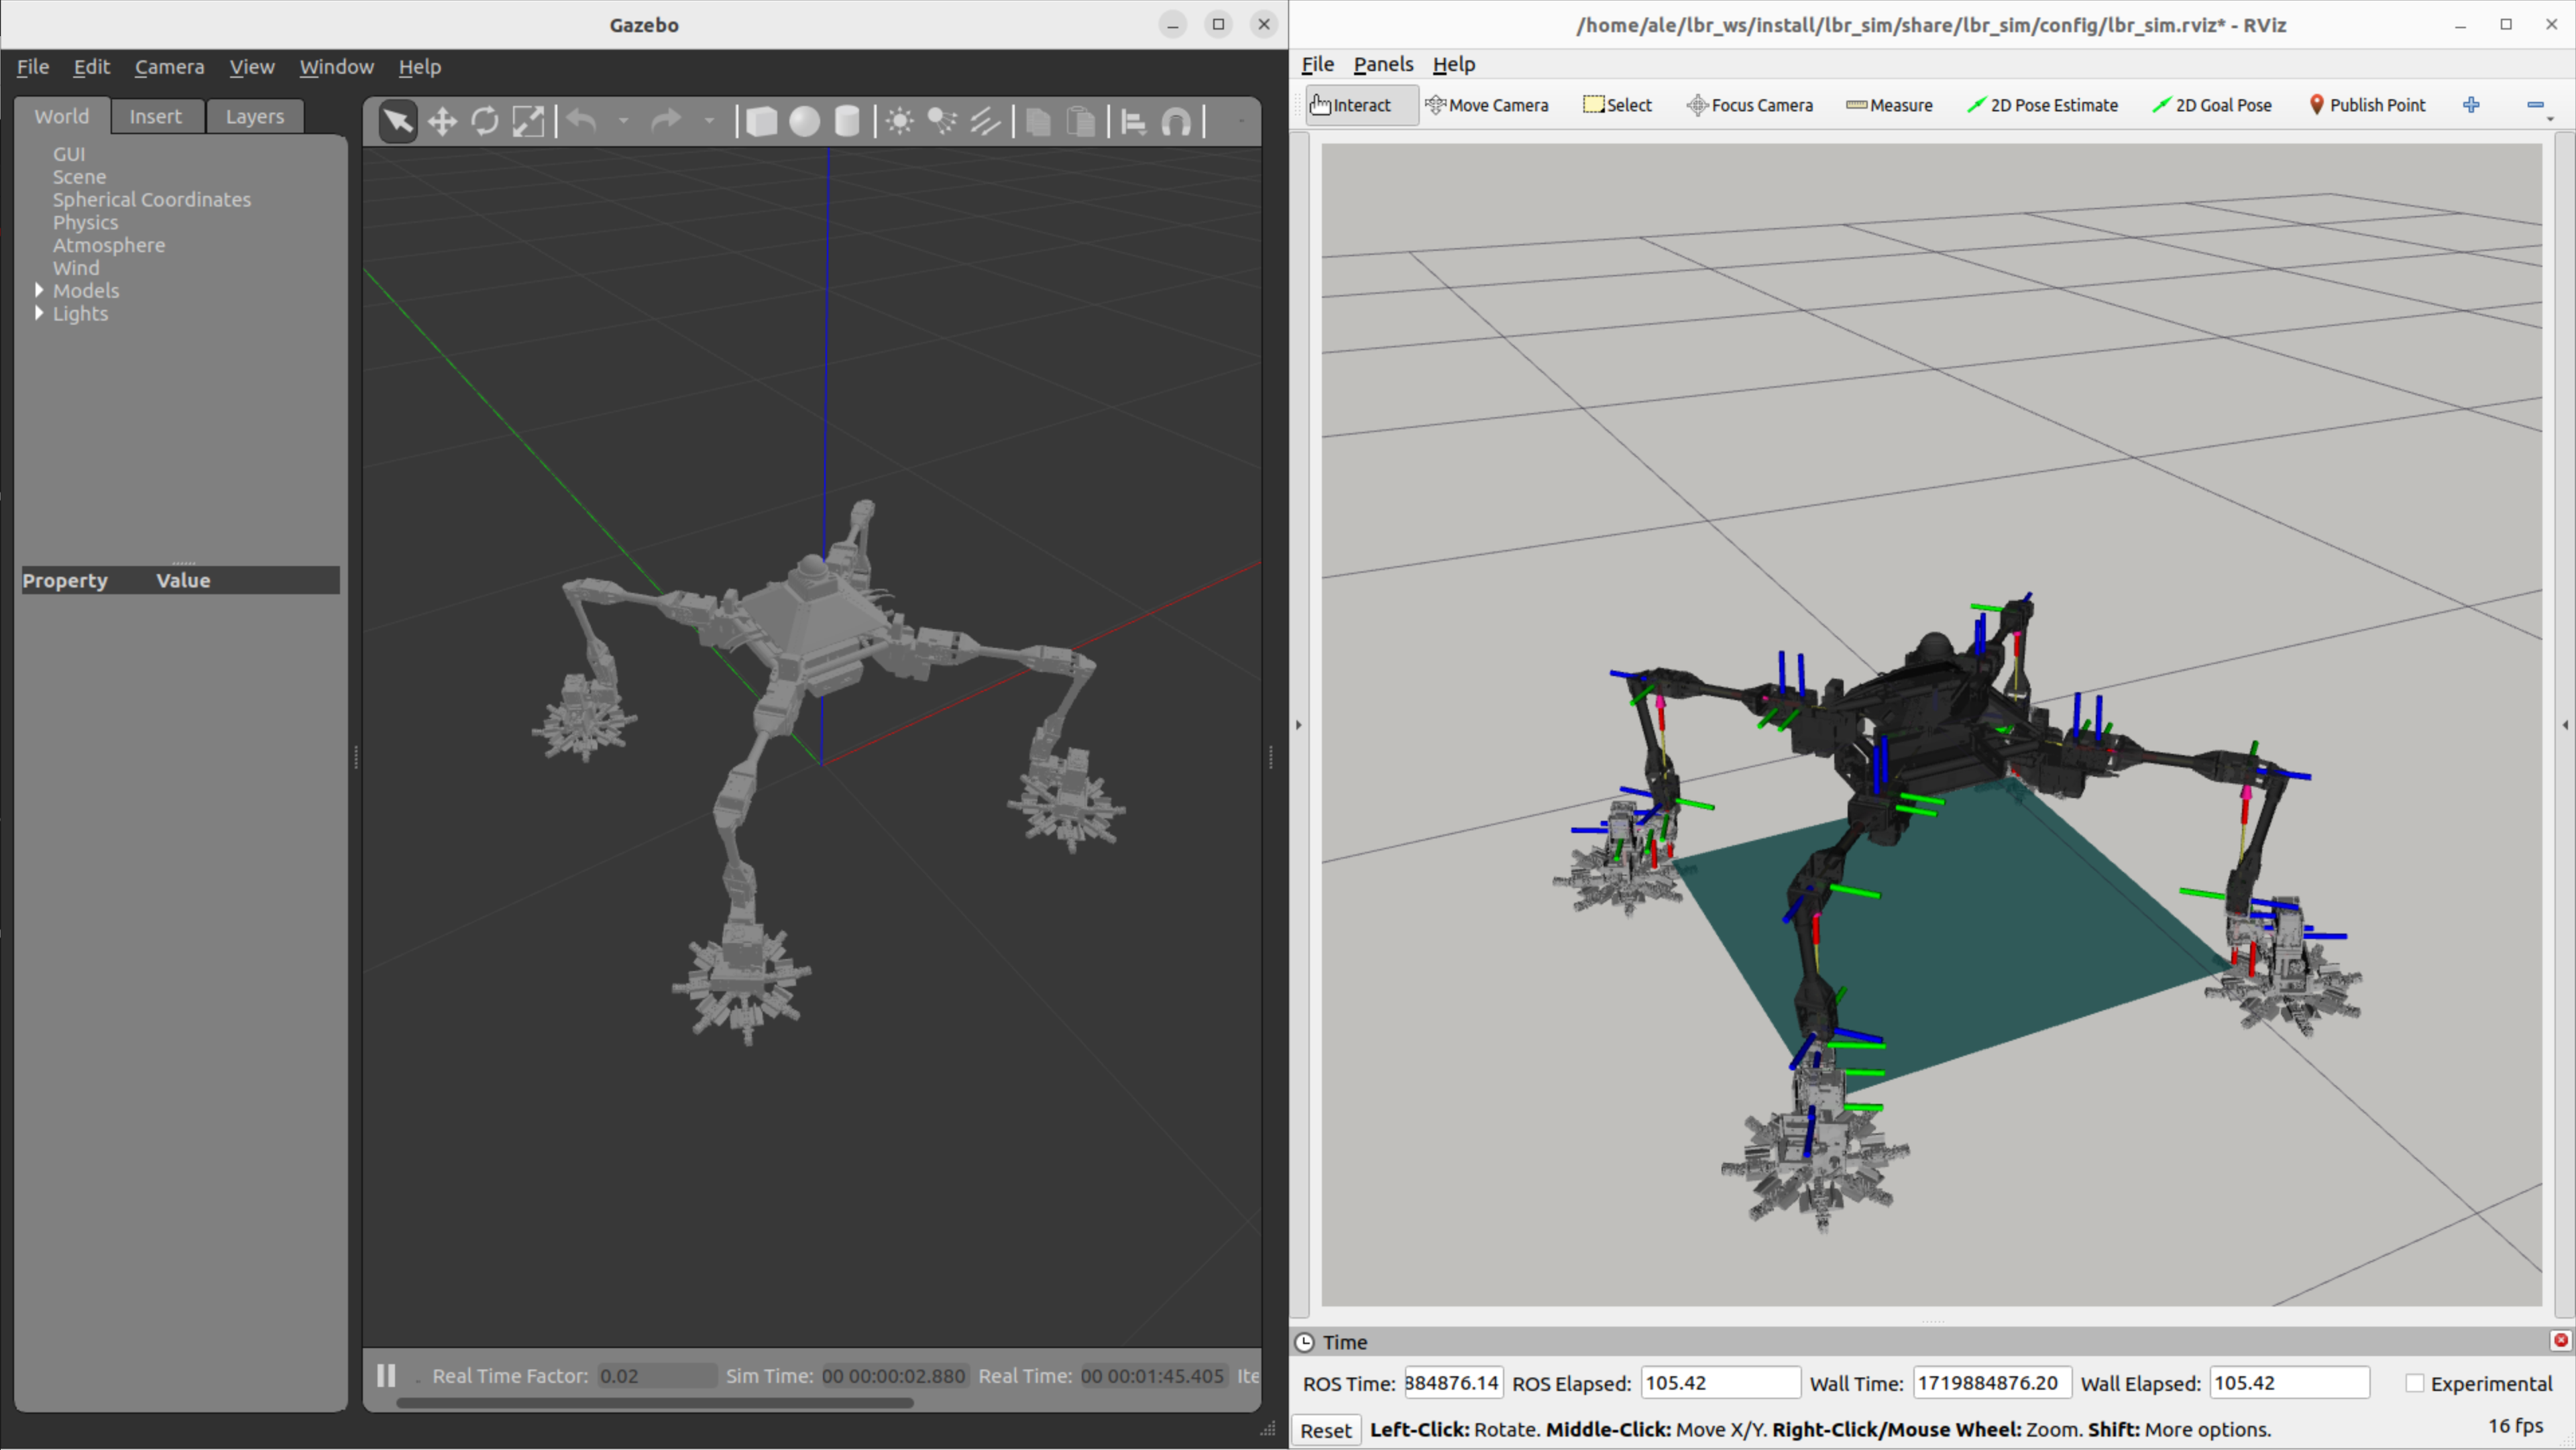
\includegraphics[width=0.4\textwidth]{Images/img_ch4/Classic_Gripper.png}}\quad
    \subfloat[Wheel mode\label{fig:sim_classic_b}]{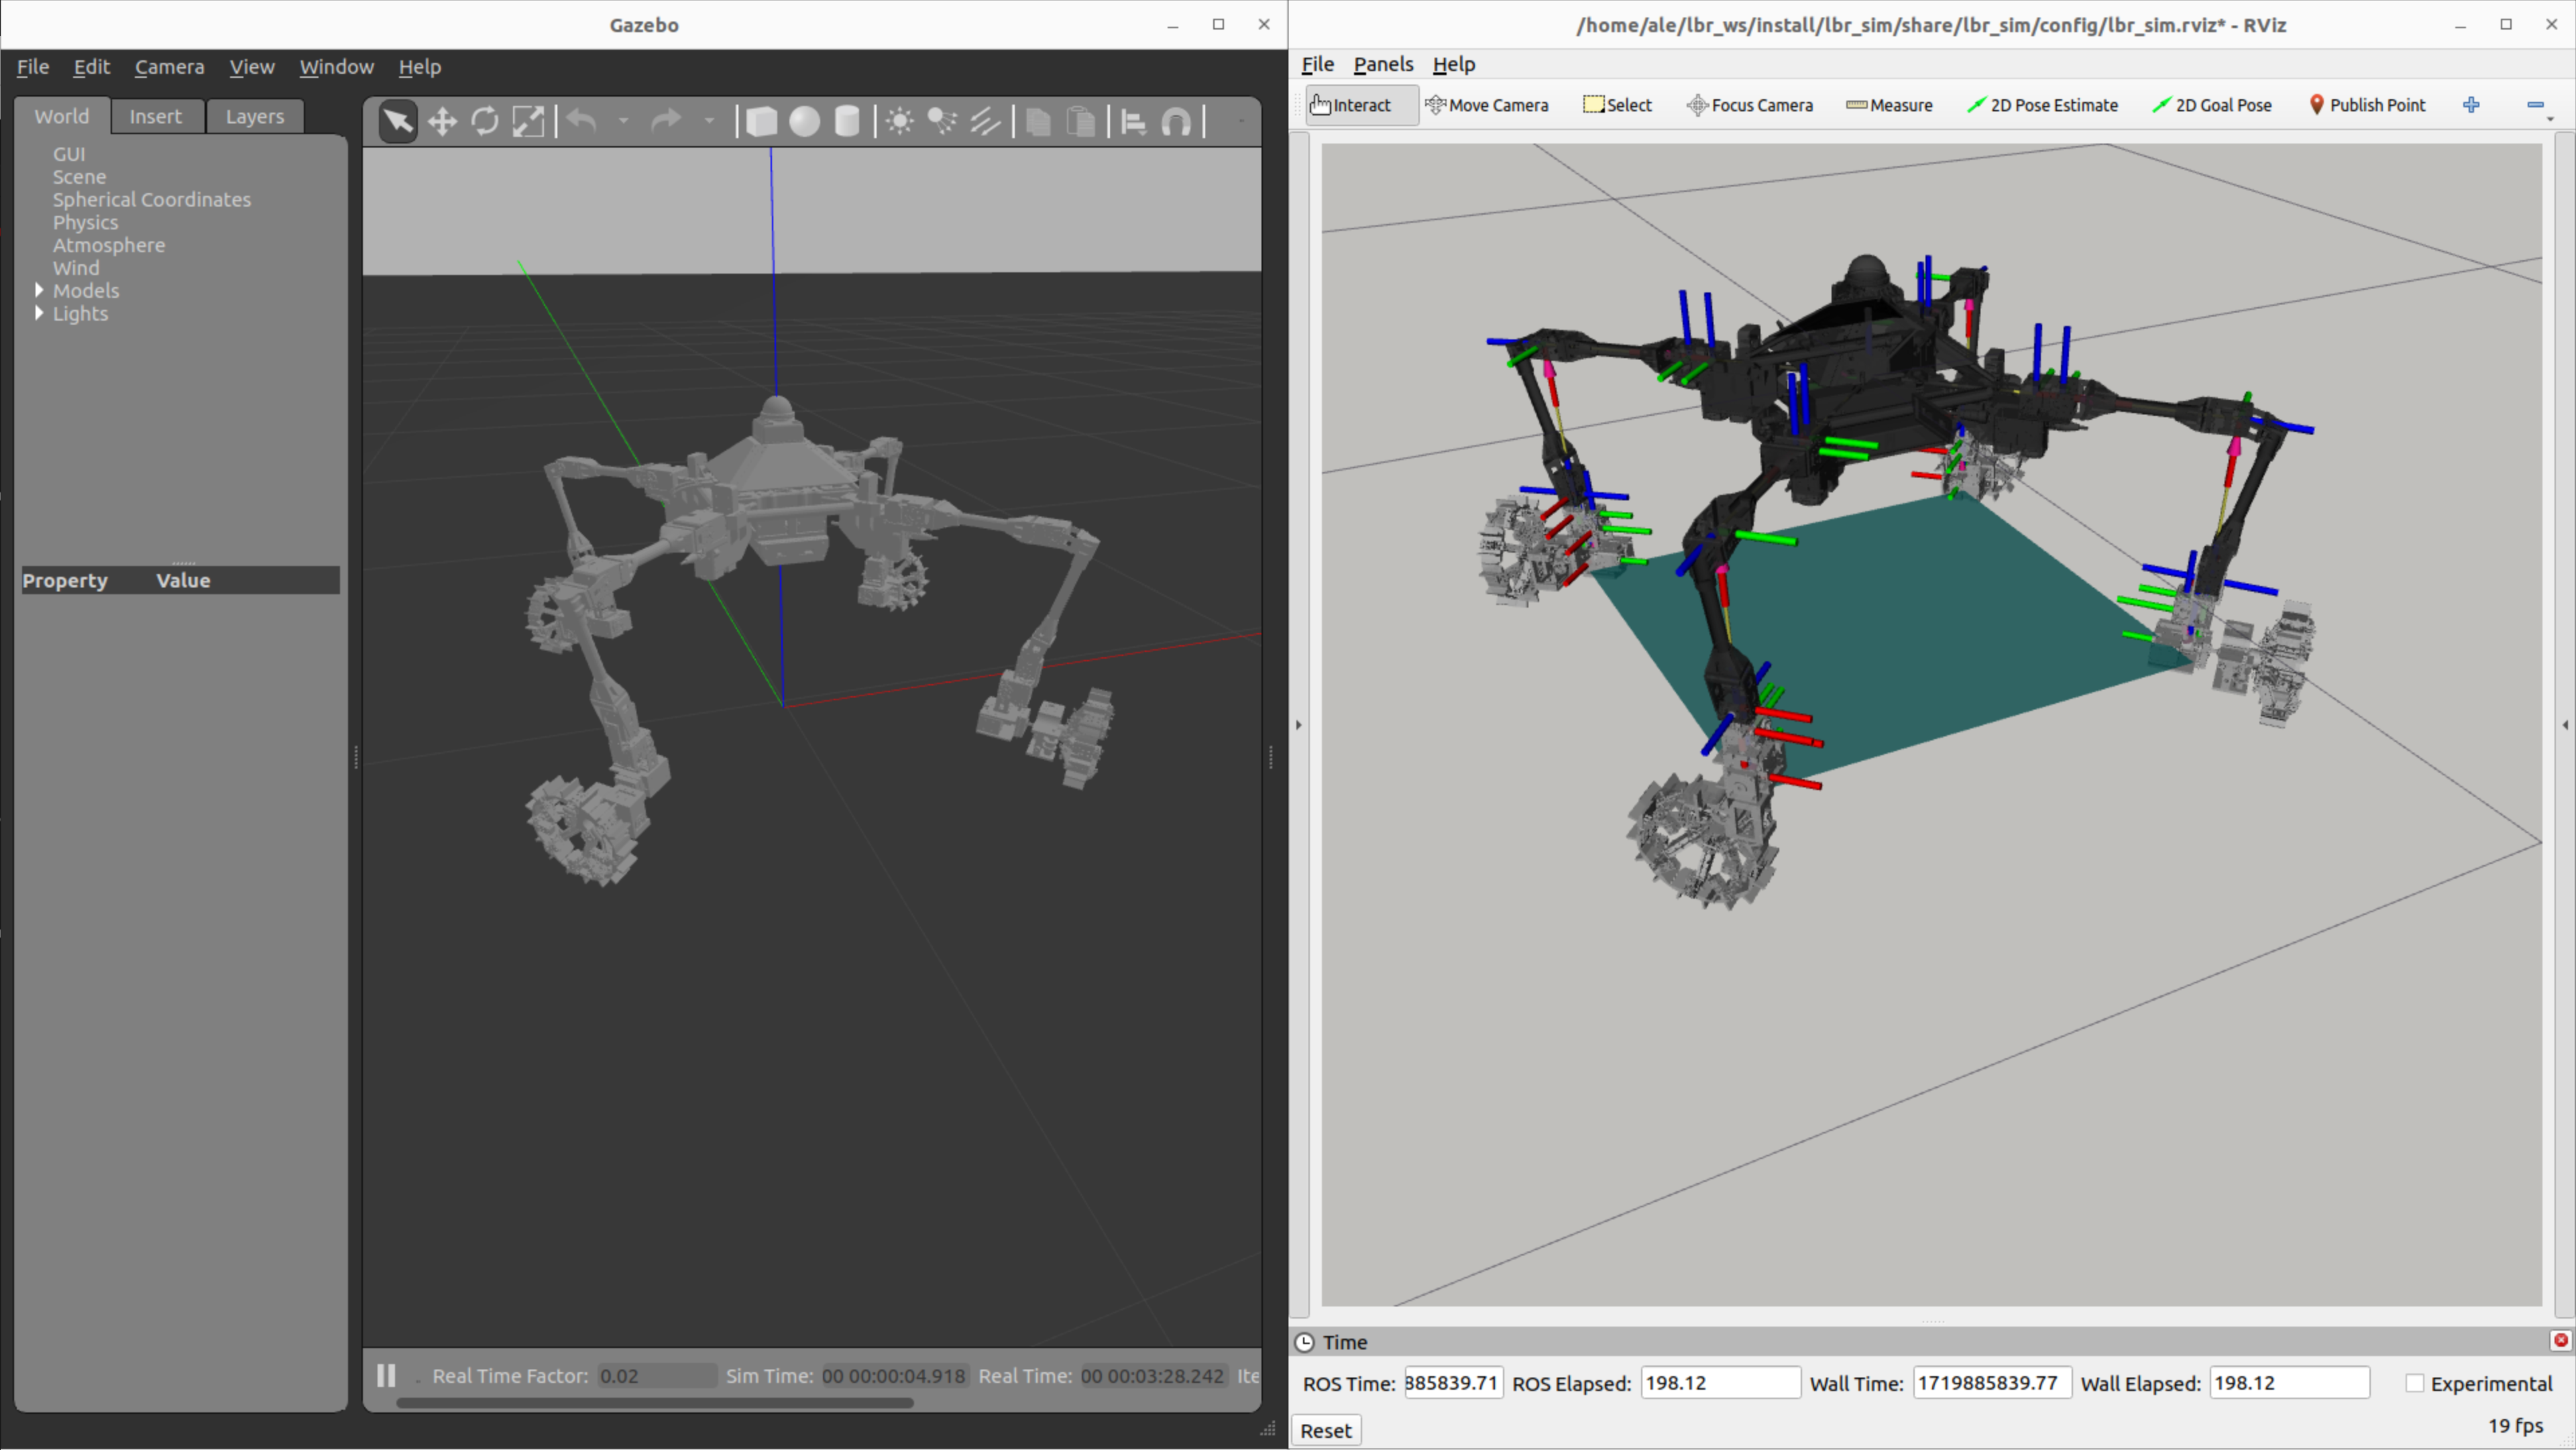
\includegraphics[width=0.4\textwidth]{Images/img_ch4/Classic_Wheel.png}}\\
    \subfloat[Mars environment\label{fig:sim_classic_c}]{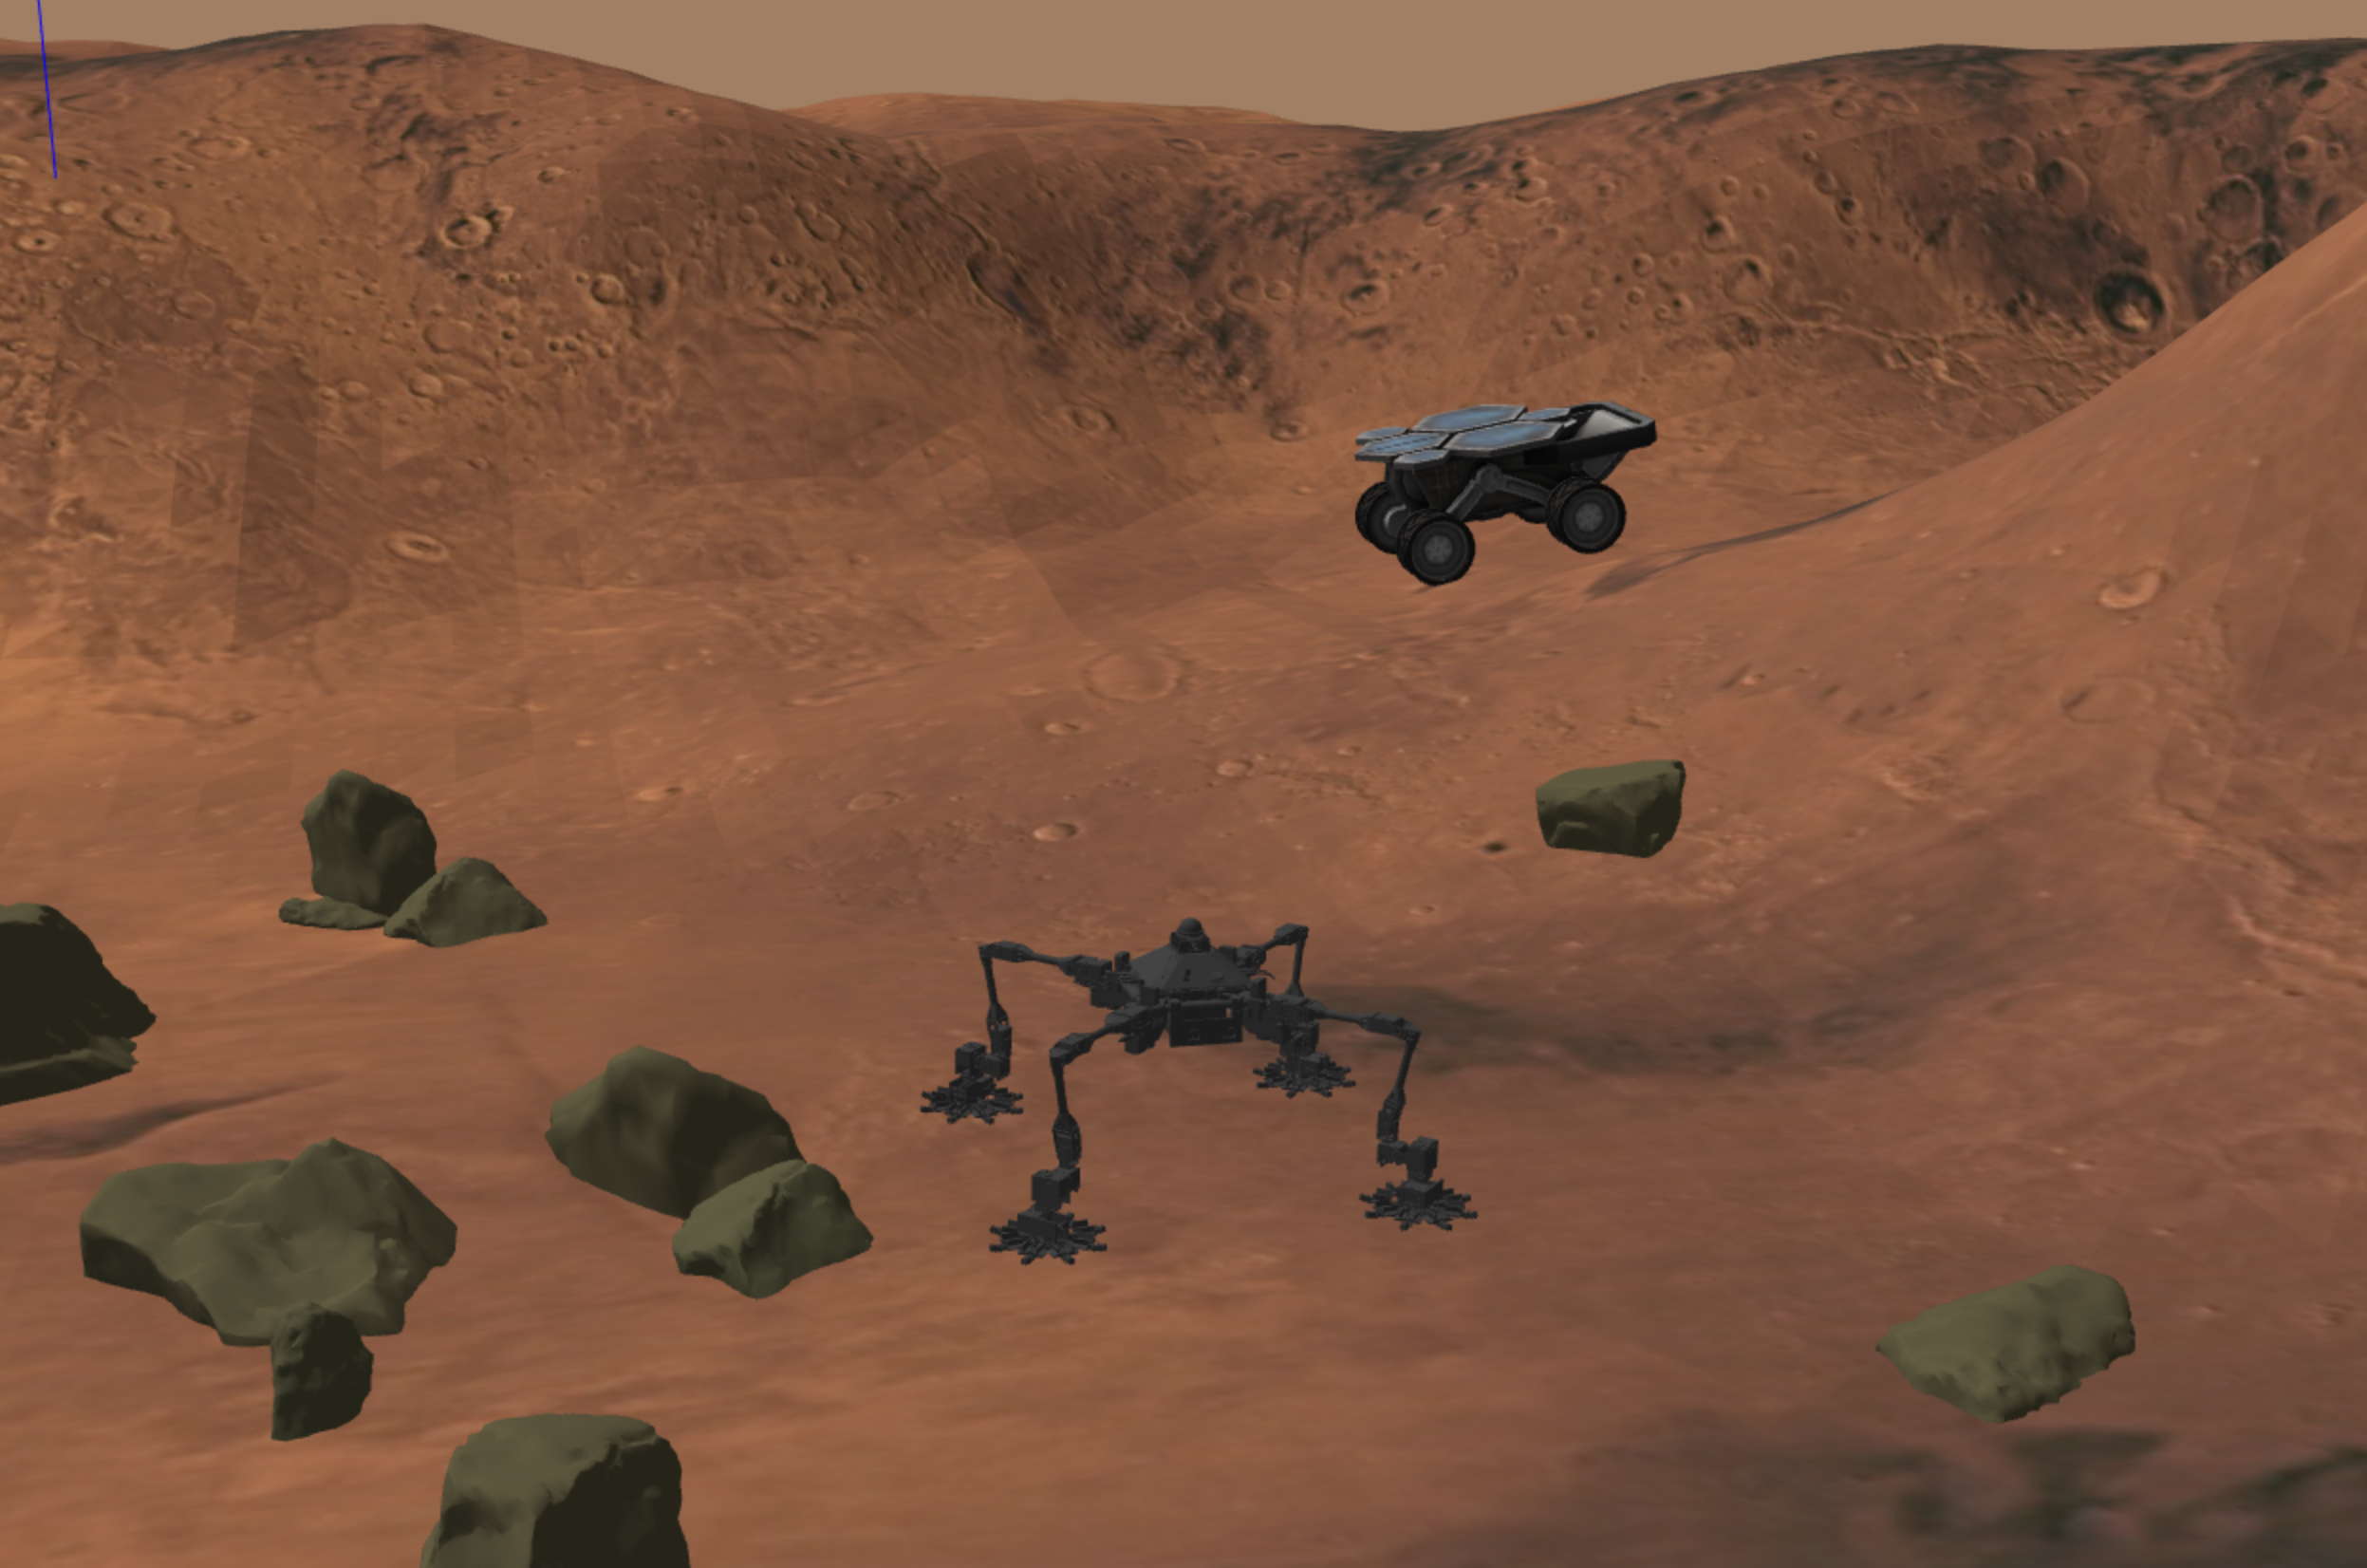
\includegraphics[width=0.8\textwidth]{Images/img_ch4/simulation_gz_classic_ex1.png}}
    
    \caption[Simulation in Gazebo Classic]{Simulation in Gazebo Classic}
    \label{fig:sim_classic}
\end{figure}

\begin{figure}[H]
    \centering
    \subfloat[Gripper mode\label{fig:sim_harmonic_a}]{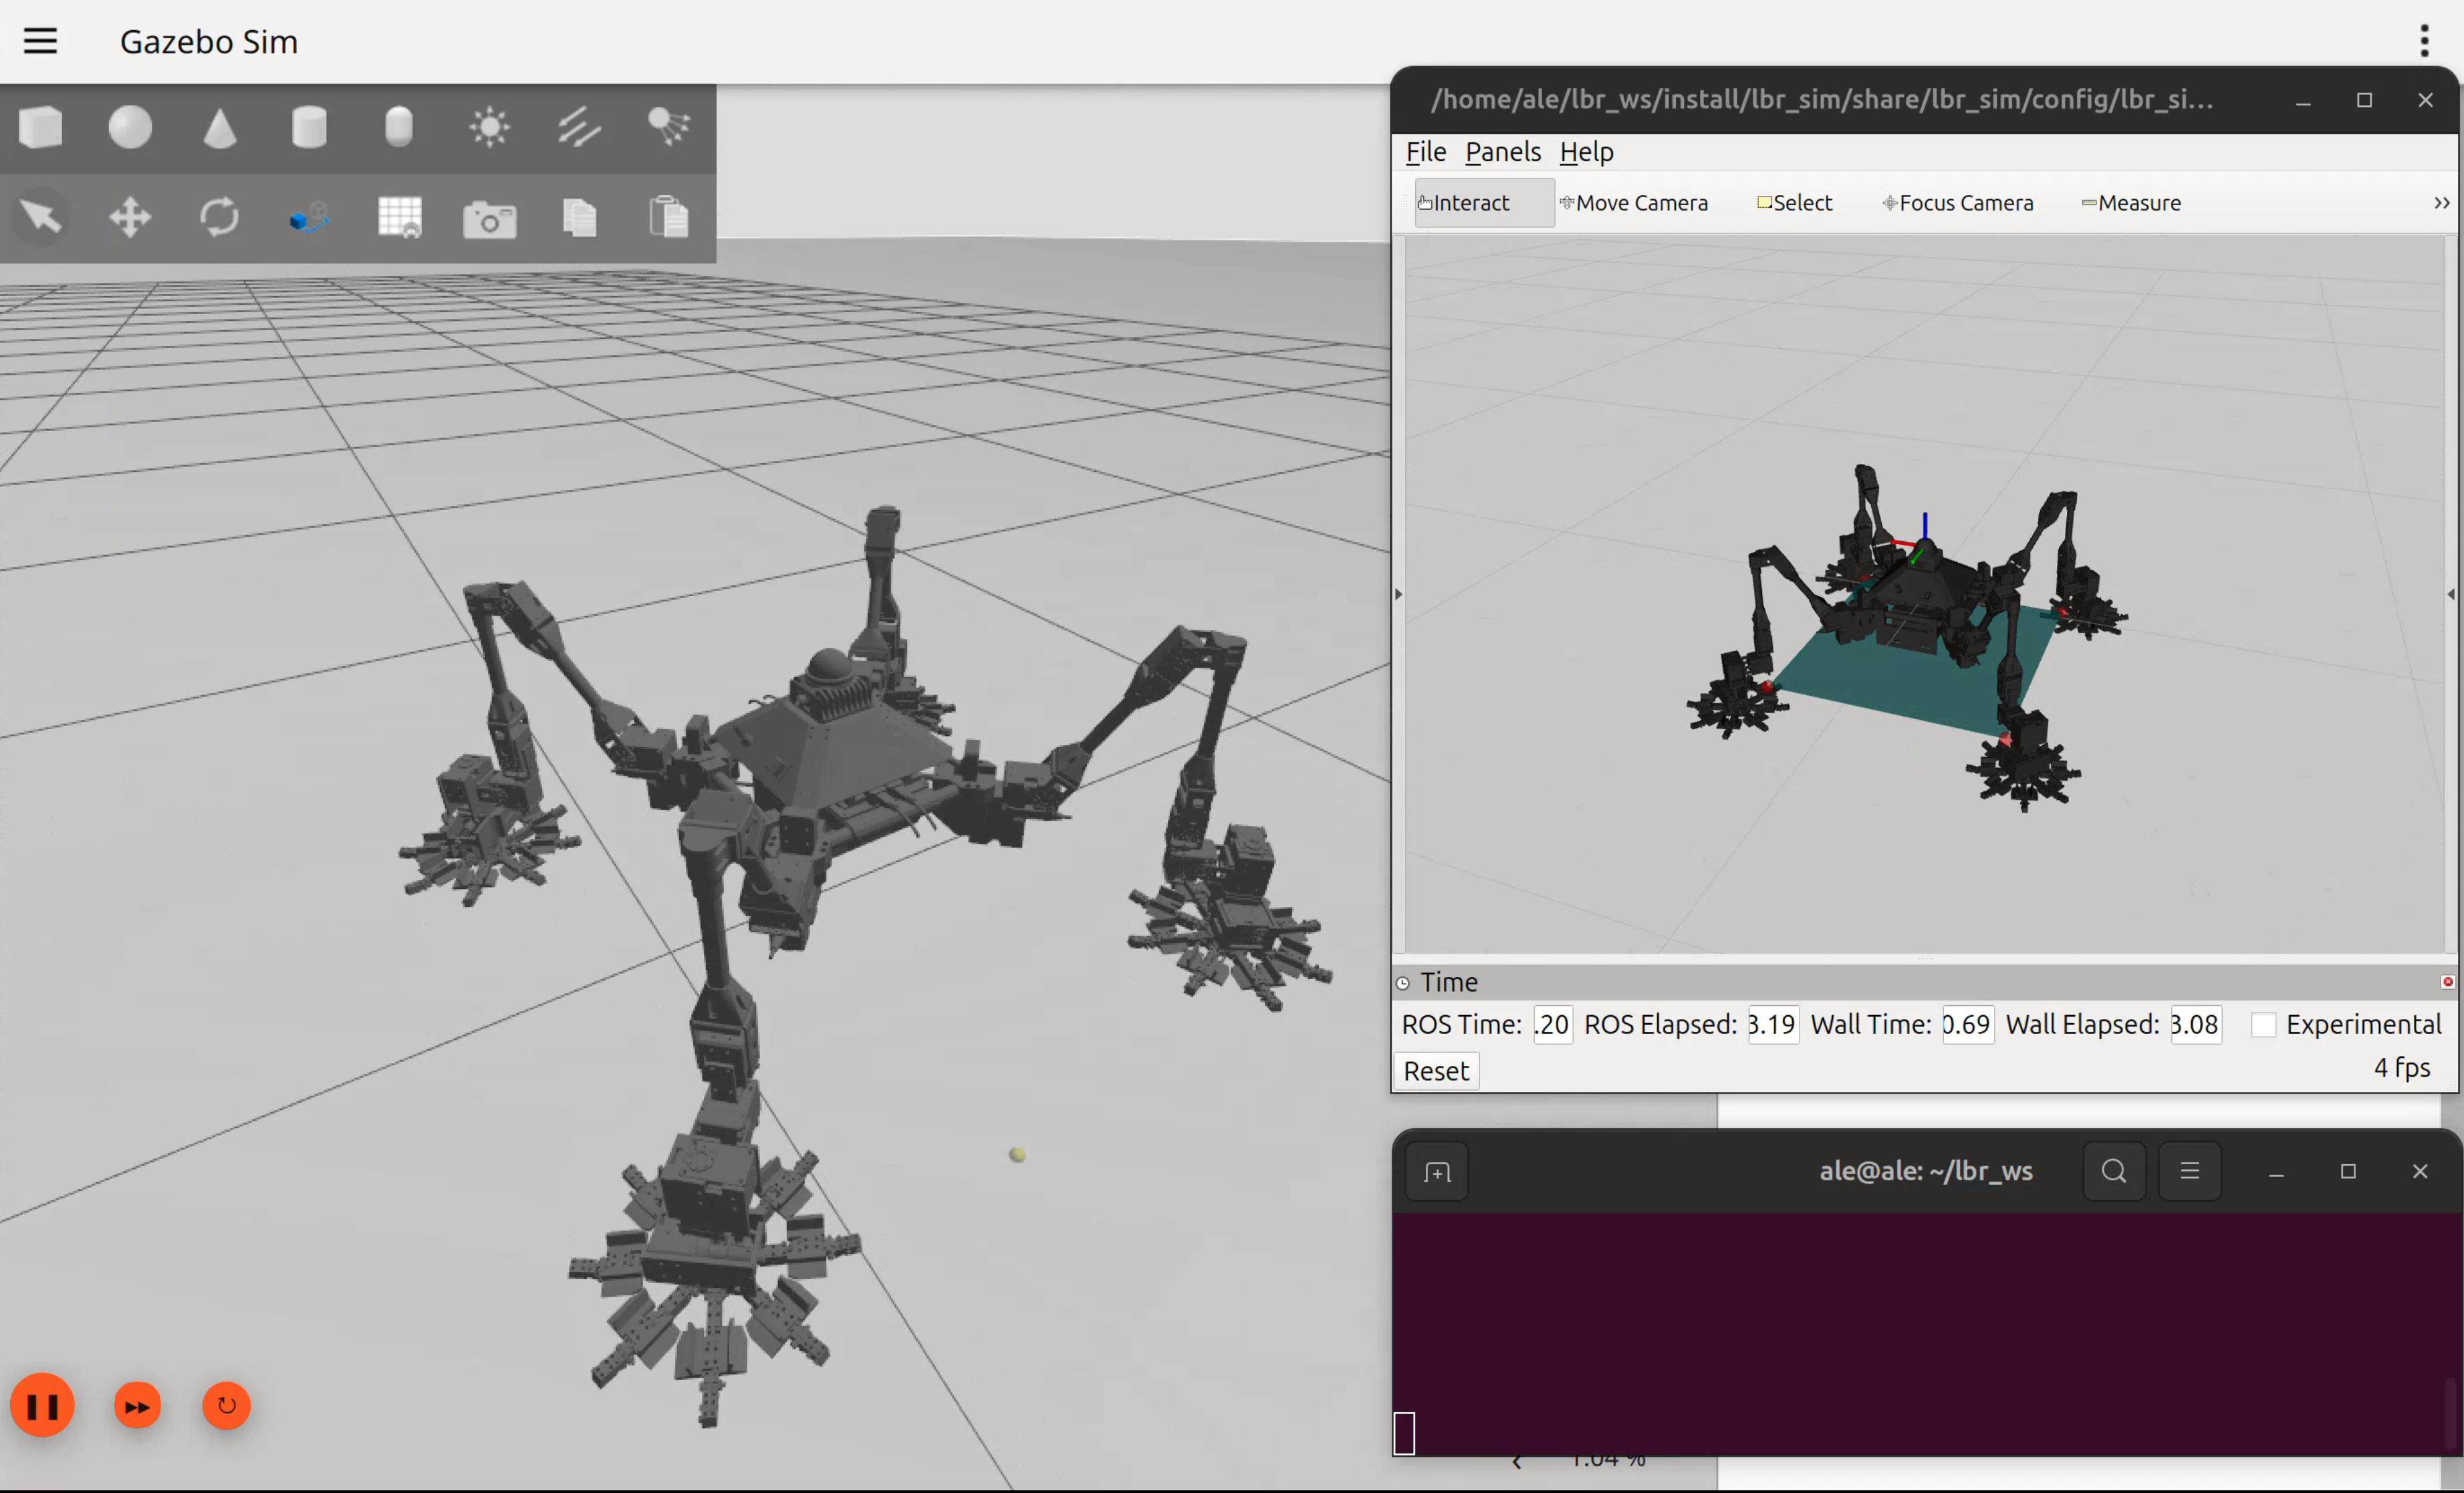
\includegraphics[width=0.40\textwidth]{Images/img_ch4/Harmonic_Gripper.png}}\quad
    \subfloat[Wheel mode\label{fig:sim_harmonic_b}]{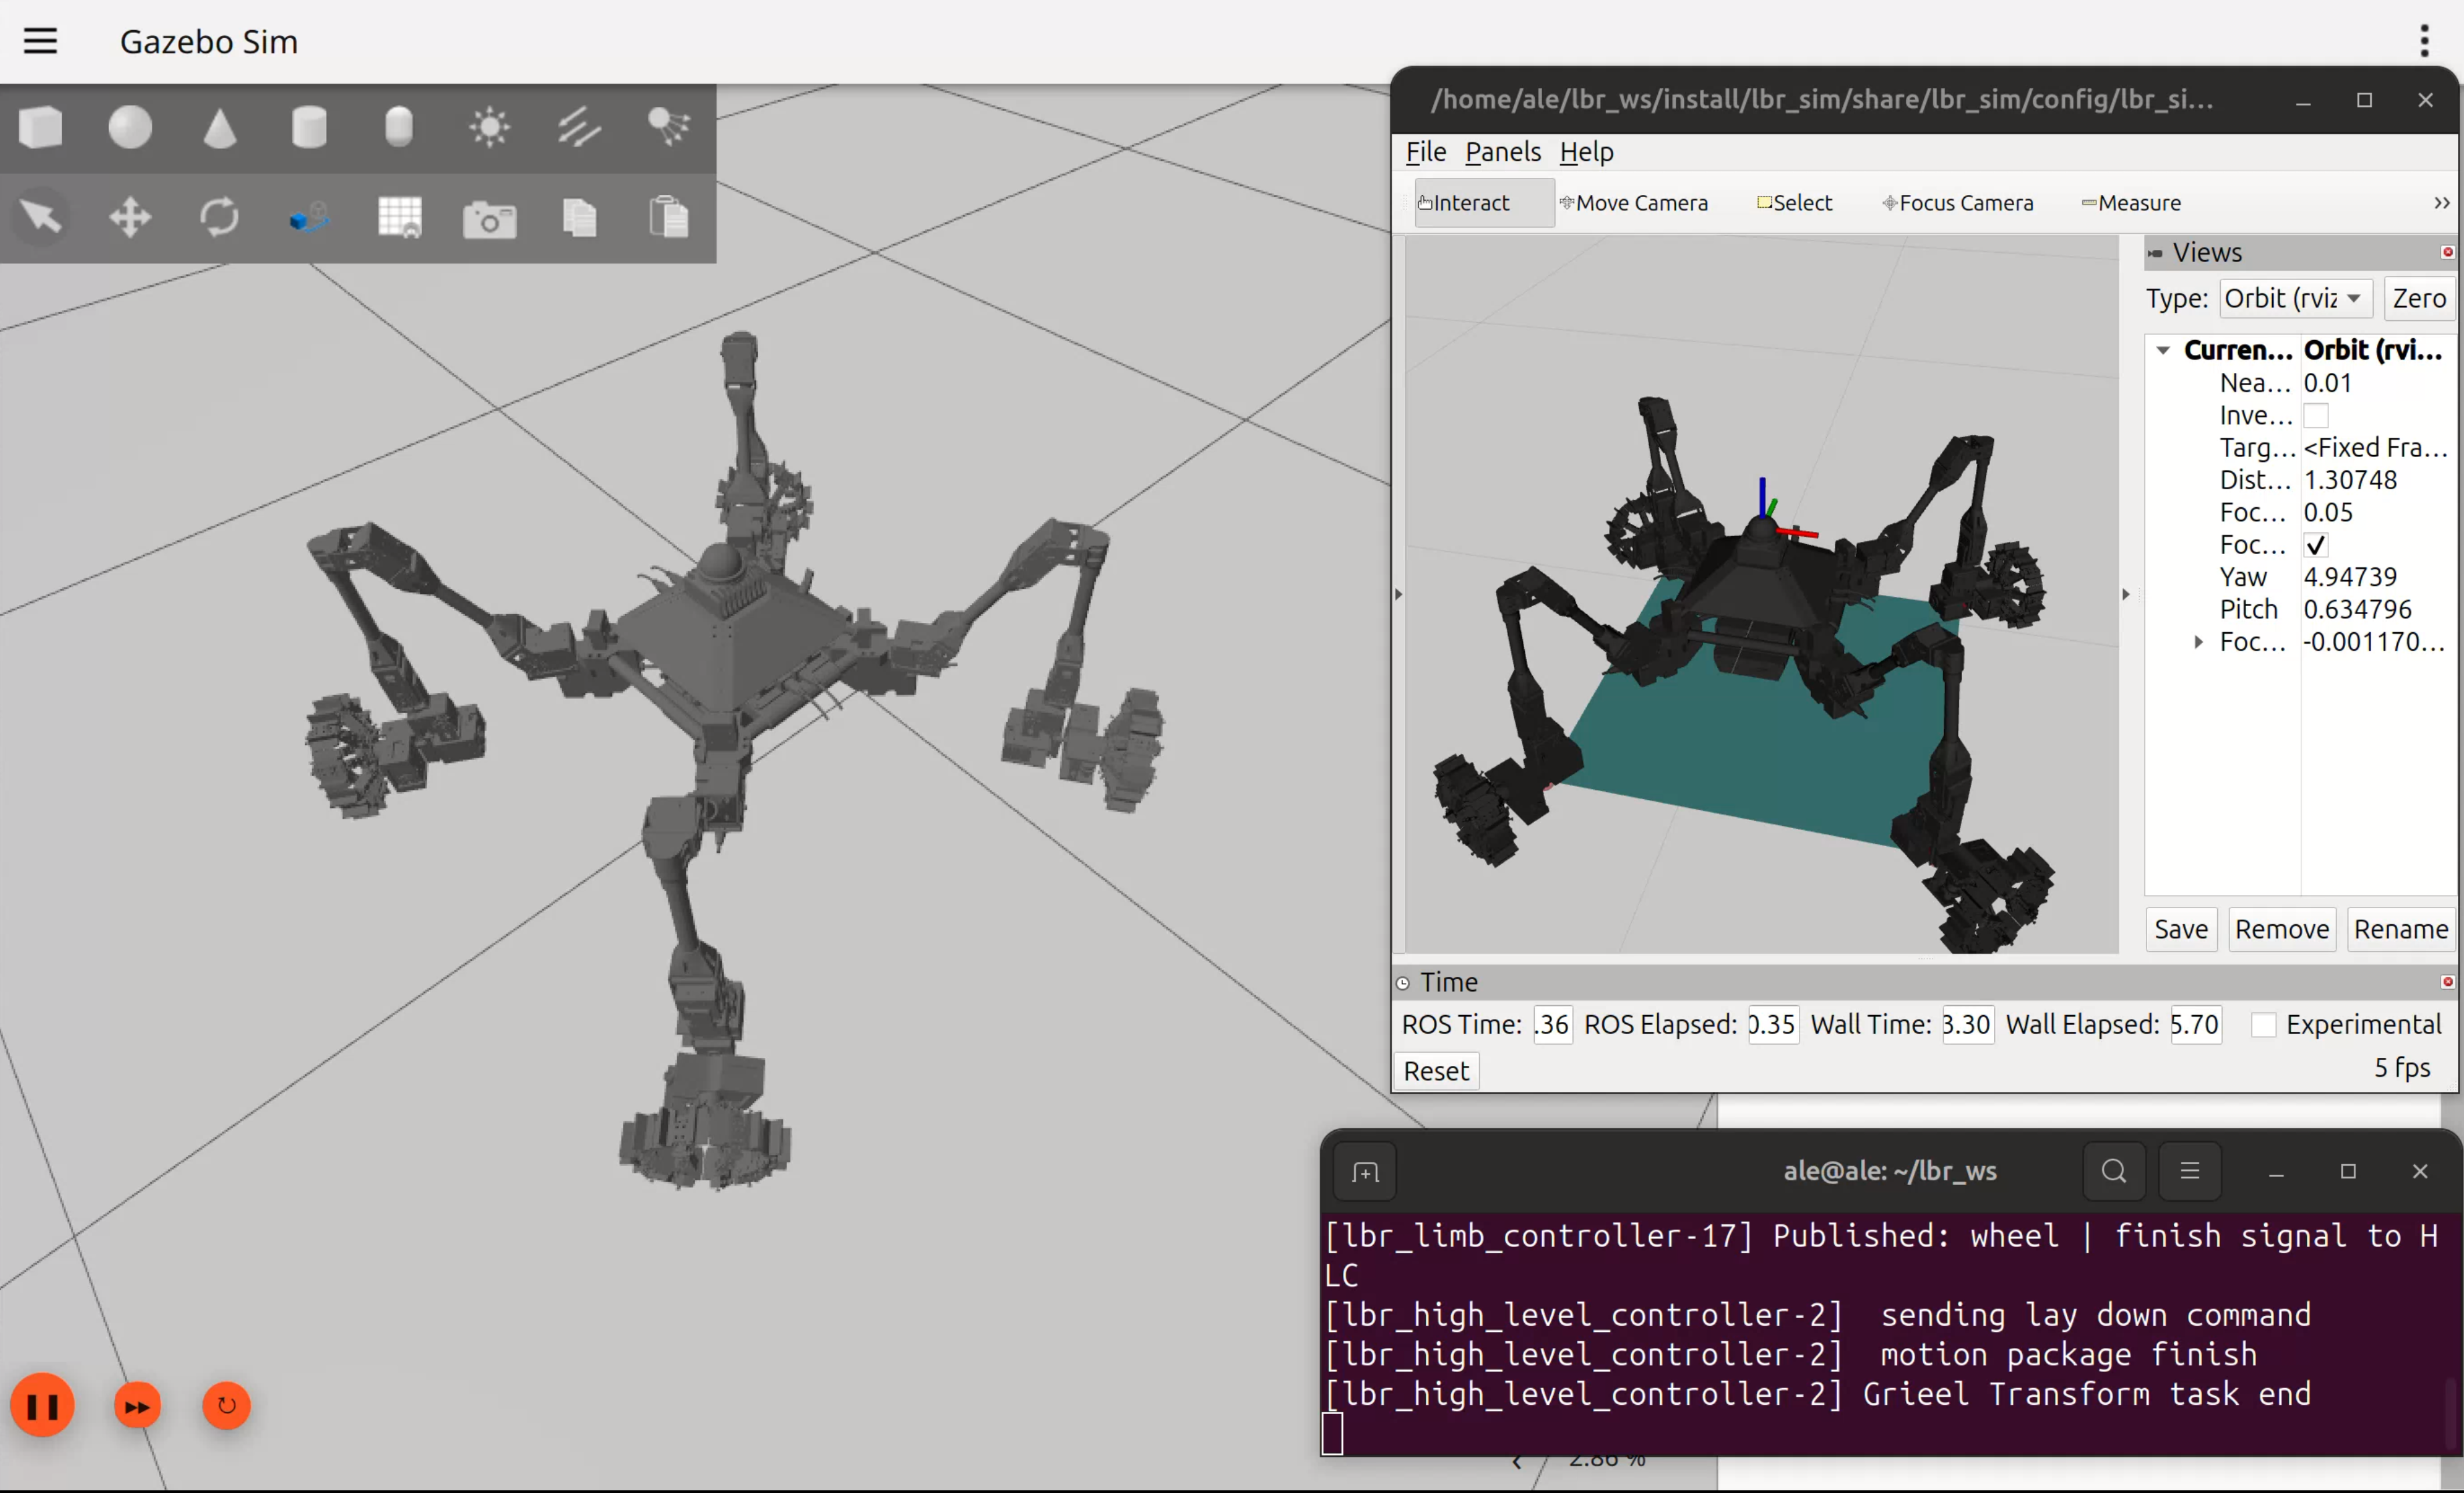
\includegraphics[width=0.40\textwidth]{Images/img_ch4/Harmonic_Wheel.png}}\\
    
    \subfloat[Mars environment\label{fig:sim_classic_c}]{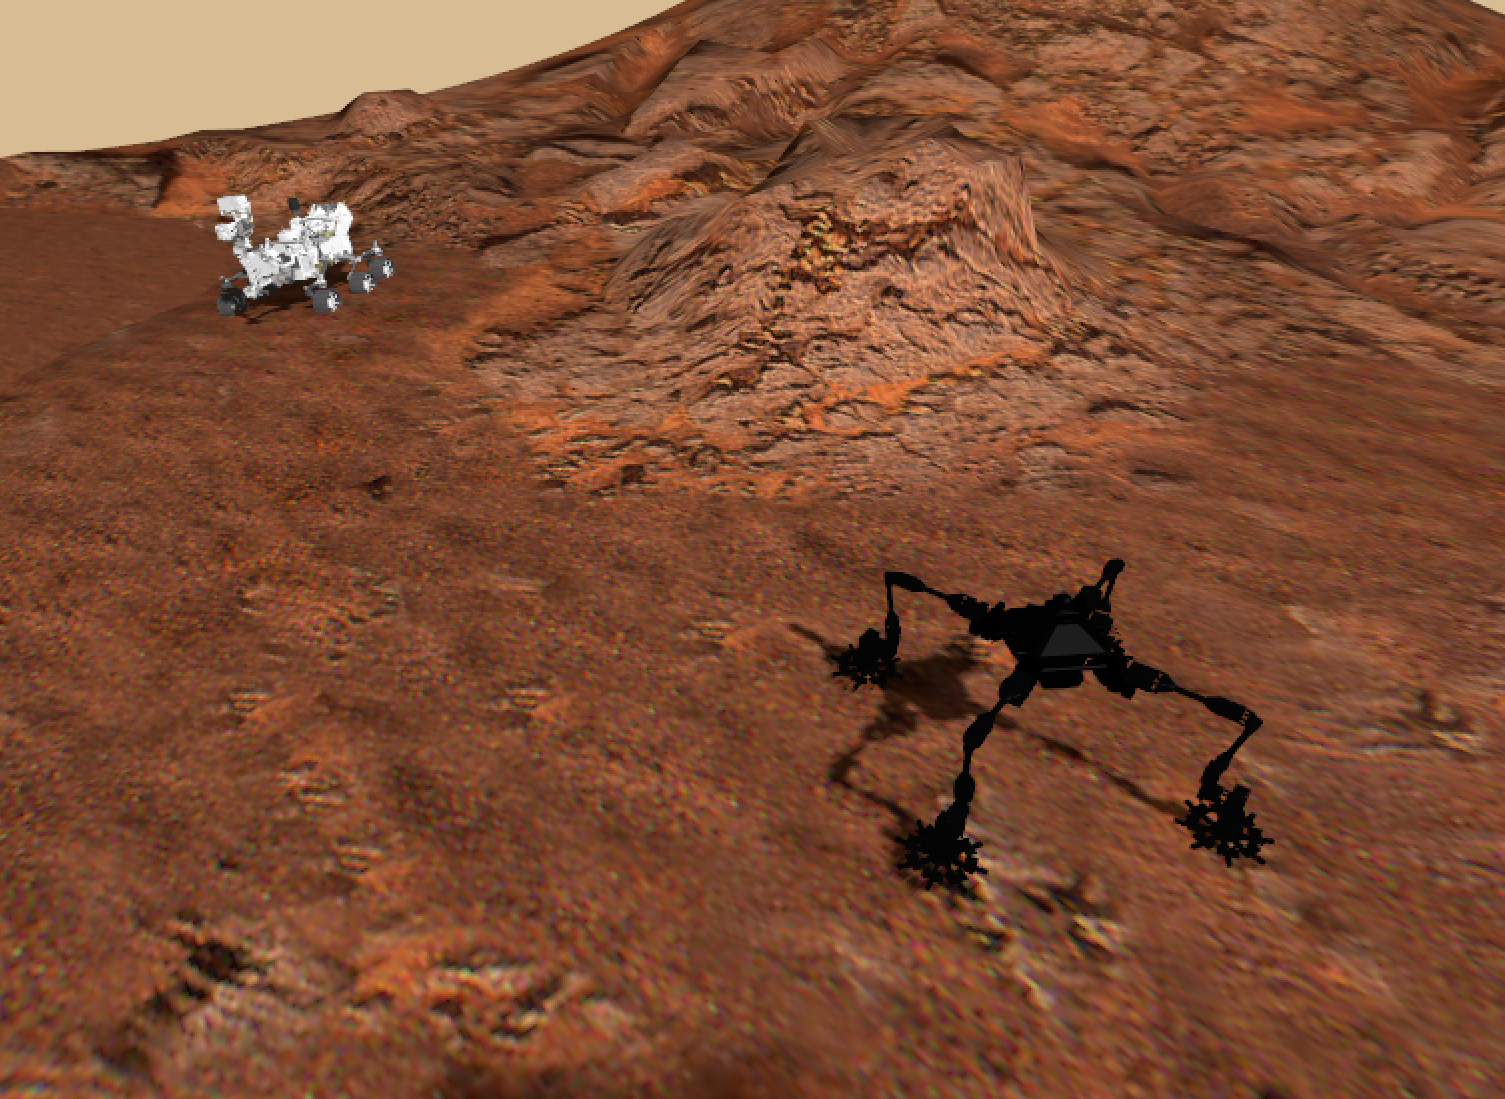
\includegraphics[width=0.8\textwidth]{Images/img_ch4/simulation_gz_sim_ex1.png}}
    
    \caption[Simulation in Gazebo Harmonic]{Simulation in Gazebo Harmonic}
    \label{fig:sim_harmonic}
\end{figure}

\subsection{MATLAB-Simulink Simulation}
\label{sec:matlab}

To improve the performance of joints' controllers, and test additional components on the controller, such as anti wind-up, filters, and feed-forward actions,  MATLAB provides the tools to perform analyses in the Laplace domain.
Simulink, a block diagram environment built on top of MATLAB, is a powerful tool for model-based control design and simulation. 

The first iterative tuning approach for the JTC, conducted in the Gazebo simulation environment (described in chapter \ref{sec:ros2_control}), was improved with a model-based approach in MATLAB-Simulink. Furthermore, the design of the IJC is based on the tests done in Simulink. 

To initialize the new simulator, the URDF model of the single LIMBERO-GRIEEL limb has been converted in DH format (reported in Fig\ref{fig:limbero_grieel_DH}), and represented as a robotic arm, with the convention used in the robotics toolbox by P.Corke\cite{CorkeMATLAB}.
% Some details on this convention transformation are described in Appendix\ref{ch:appendixA}, many tools to analyze serial links robotic structure exist, and this URDF to DH conversion has been an important aspect. 

After defining the limb model, it is possible to derive the dynamical matrices appearing in (\ref{eq:ManipulatorEoM}) and use it for model-based controller tuning.
Then, import the limb in Simulink and set up a block diagram for the motion control where testing its performance is simple. 

This approach considers only one limb and doesn't take into account the complex closed chain structure of LIMBERO-GRIEEL robot. 
Methods to implement a complex tree structure as a limbed robot and simulate it exist, with toolboxes such as the Robotic System Toolbox, based on Simscape Multibody.
Under the assumption of a high reduction ratio, the decoupled model described in section \ref{sec:DecoupledDyn} holds also for the multi-limbed structure. 
Nevertheless, because the limb behaves as a robotic arm that changes its fixed base:
\begin{itemize}
    \setlength\itemsep{-0.7em} 
    \item the limb root when not in contact
    \item the ground contact point if in contact
\end{itemize}
 a 2-state switching dynamic model has been considered for the limb. The dynamic properties change between the root-to-EE (raised) and the contact-to-root (in contact), and both models have been defined in MATLAB and tested. Further details on this aspect are given in the chapter \ref{sec:IJC} where the tuning approach is summarized.

The Simulink scheme used during control is reported in Fig.\ref{fig:Simulink} below, and the IJC is based on the scheme of Fig.\ref{fig:PPI_IJC}, with some additional components. 

\begin{figure}[H]
    \centering
    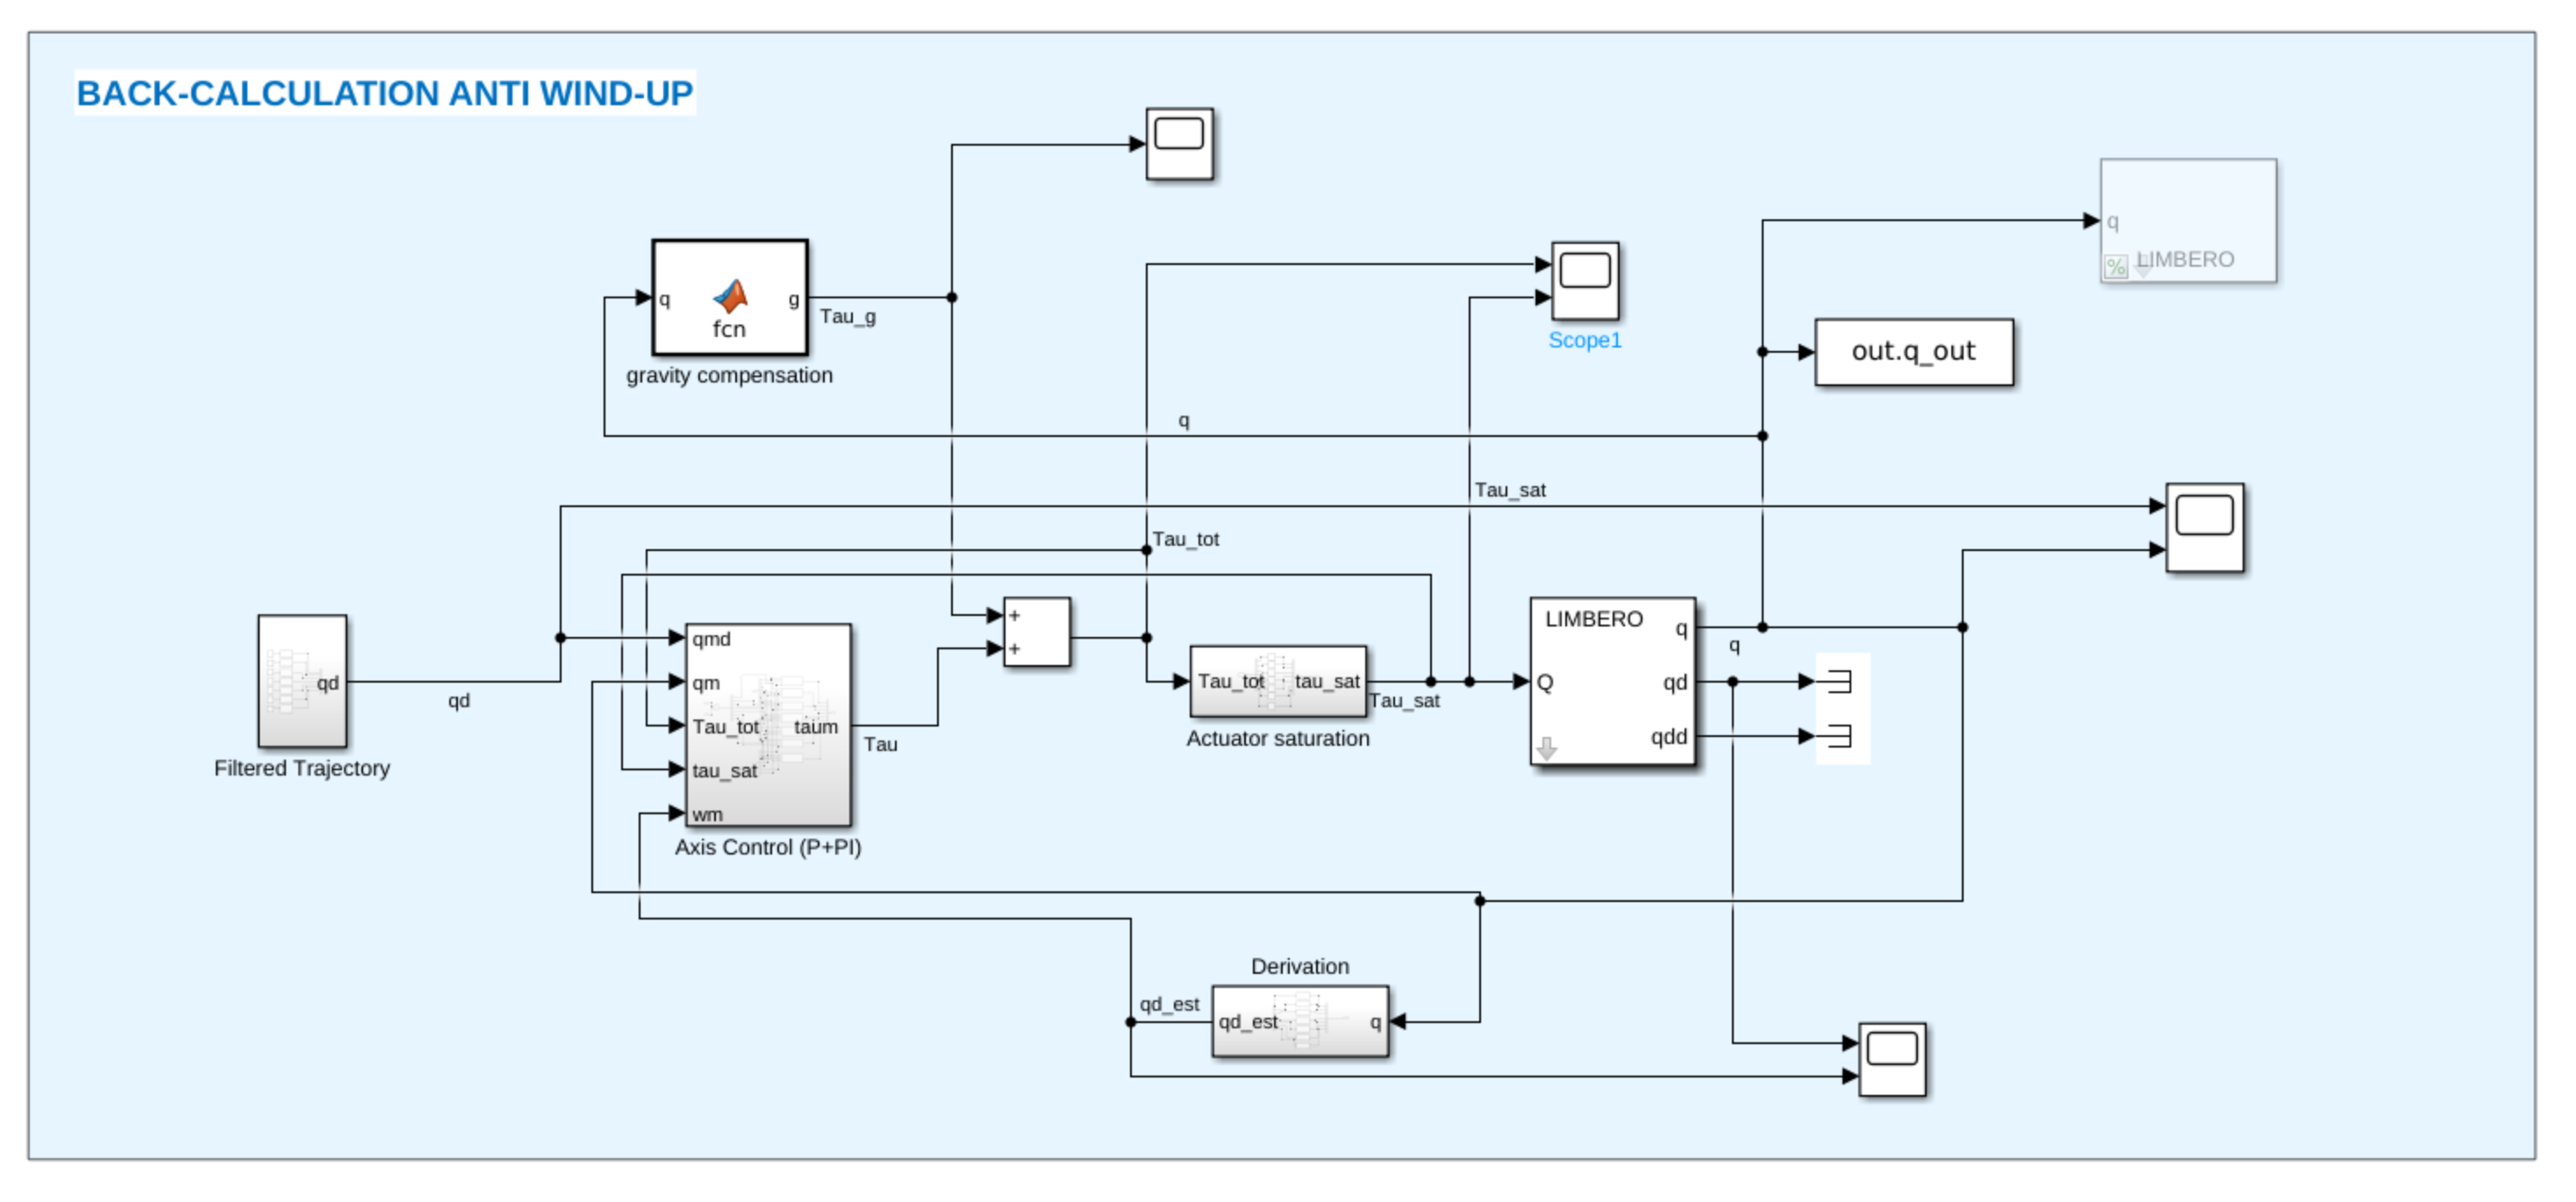
\includegraphics[width=1.1\textwidth]{Images/img_ch4/Simulink.png}
    \caption{Simulink scheme used to test single limb IJC performance}
    \label{fig:Simulink}
\end{figure}

Finally, MATLAB has been used to define a kinematic model of LIMBERO-GRIEEL and implement simple base task and limb tasks computation, used to test the BME theory derived in section \ref{sec:base_manipolability} and improve the transition algorithm described in the next section.




\clearpage
\thispagestyle{empty} % This removes the header/footer but keeps the numbering
\vspace*{\fill} % Pushes everything to the bottom
\newpage
\BlankPageTLGWthree
\chapter{GRIEEL Transition Algorithm}
\label{ch:chapter_five}%

This chapter introduced the principal contribution of this research, which has inspired the BME theory (discussed in \ref{sec:base_manipolability}). 
The tools to model, control, and analyze the performance of multi-limbed robots, and the description of LIMBERO-GRIEEL (L-G) are fundamental for defining an efficient transformation algorithm.

The multimodal locomotion capabilities of L-G require a seamless transition between two functional modes:  a wheeled locomotion system and a versatile gripper for manipulation and walking/climbing tasks.
Furthermore, hybrid configurations are considered, such as limbs in wheel mode used for driving and others in gripper mode to manipulate the environment and carry objects. 

The final objective is the definition of an efficient and stable algorithm to perform the transition of locomotion mode for L$-$G, in terms of motion planning and control. 

Additionally, the reusability and modularity of this procedure have been an additional requirement. 
In fact, GRIEEL's potential goes beyond its usage as LIMBERO's EE, making its design, control system, and related procedure adaptable for any limbed robotic system is the ultimate goal.   

First, the previous procedure used to perform this locomotion transition is described, and the limitations are discussed. 
Then, the new algorithm is defined, and the base motion sequence is analyzed using the novel BVME. 
Finally, the advantages of the proposed algorithm are highlighted. 
The higher-level components that decide when and what type of transition is needed goes behind this research, in any case, once developed are easy to integrate on the system. 

\section{Previous Transformation Procedure}
\label{sec:old_algorithm}

The procedure defined by M.Uda\cite{GRIEELUdaThesis} to perform locomotion mode transition is reported in Fig\ref{fig:GRIEEL_oldTransition}, with the relative timeline.
This motion sequence, responsible for the driving-to-walking locomotion transition, starts at $t=20s$ and ends at $t=120$, with the following steps: 
\begin{enumerate}
    \setlength\itemsep{-0.7em} 
    \item\label{item:old_1} Lay the base on the ground.
    \item\label{item:old_2} Complete W2G transition for all modules, releasing tethers tension. 
    \item\label{item:old_3} Raise all the limbs 
    \item\label{item:old_4} change wrist configuration. 
    \item\label{item:old_5} Stand up, maintaining the LF leg raised, ready for walking. 
\end{enumerate}
The opposite walking-to-driving transition is defined with a similar sequence, except for steps (\ref{item:old_3}) and (\ref{item:old_5}). In (\ref{item:old_3}) a different wrist configuration is defined in the case of module G2W transition.For step (\ref{item:old_5}), if driving is the upcoming locomotion mode, all limbs (in wheel mode) are kept in contact with the ground. 
\begin{figure}[H]
    \centering
    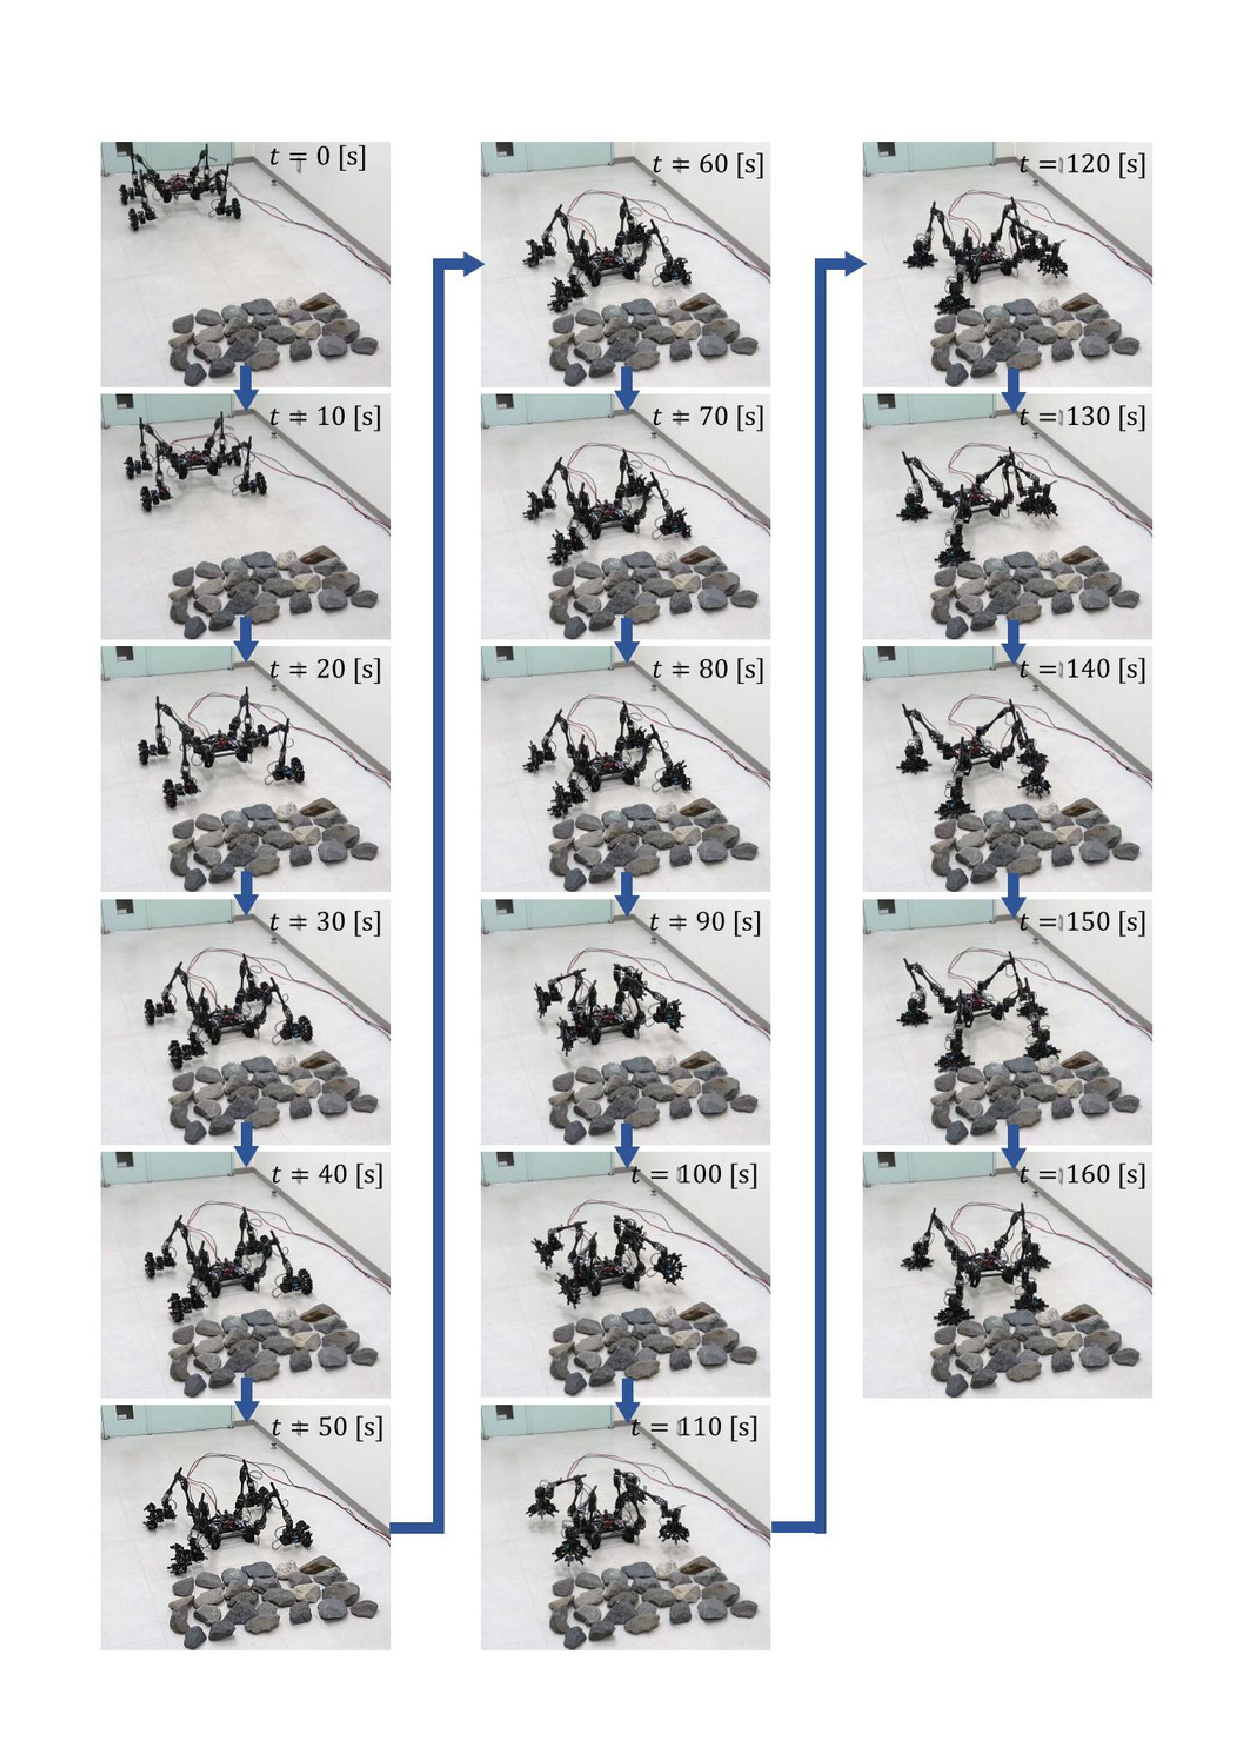
\includegraphics[width=0.65\textwidth]{Images/img_ch5/GRIEEL_oldTransition.pdf}
    \caption{\cite{GRIEELUdaThesis}Driving to walking locomotion transition with the previous algorithm (transformation of all limbs W2G).}
    \label{fig:GRIEEL_oldTransition}
\end{figure}
This sequence is completed in a small amount of time, with reduced energy consumption, and is easy to define. However, it has the following limitations:
\begin{itemize}
    \setlength\itemsep{-0.7em} 
    \item[\textbf{a)}] \label{item:problem_a} A horizontal support plane is required when laying down the base, to avoid any possible tumbling problems. Furthermore, unexpected rocks or small sharp obstacles could damage the bottom of the base, where batteries and other electronics are exposed (One possible solution to this could be a redesign of the robot base. However, this is against the reusability requirements described previously).   
    \item[\textbf{b)}] \label{item:problem_b} It is not the best sequence for a single-limb transformation. In a transition to a hybrid configuration, as changing from full driving locomotion (4-wheeled) to 3-wheeled with one manipulating gripper, this procedure is time-consuming and not always possible. 
    
    Another case when a single transformation is needed is transitioning during locomotion. This means that the gait scheduler is involved in the transition, instead of maintaining the same pose in space during mode transformation, it is completed while moving towards the objective. This is not discussed here, but some comments are made in the last section.  
\end{itemize}

The new motion sequence is now defined, to overcome those problems and guarantee the requirements listed before. 

\section{New Transformation Algorithm}
\label{sec:new_algorithm}

In defining a new transition sequence for GRIEEL, the requirements are: 
\begin{enumerate}
    \setlength\itemsep{-0.7em} 
    \item\label{item:stability} Stability of the system. 
    \item\label{item:rough} Enabling transition even in rough terrains\\(where laying down the base may be not possible). 
    \item\label{item:slopes} Enabling transition in small sloped terrains \\(where GRIEEL's spine gripping can be exploited).
    \item\label{item:reusability} Simple to be redefined and adapted for different conditions or robotic platforms. 
    \item\label{item:single} Possibility to complete single module transitions. 
    \item\label{item:dexterity} Avoid limb configurations where the robot base's dexterity and maneuverability are degraded. 
\end{enumerate}

If all of them are respected in the definition of a new procedure, problems \hyperref[item:problem_a]{(\textbf{a})} and \hyperref[item:problem_b]{(\textbf{b})} are overcome, and the additional desired goals listed in this chapter's introduction are met. 

In this analysis, it is assumed that, when a GRIEEL mode transition is required, the terrain is flat or with small slopes, but rocks and sharp obstacles on the ground can be present. Under this assumption, SP and ZMP criteria can be used to evaluate system stability. The last section of this chapter briefly discusses possible extensions, and how simple it is to integrate them.

The main idea behind the new algorithm comes from the configuration represented in Fig.\ref{fig:limbero_grieel_mars_stable}, as an obvious solution to problem \hyperref[item:problem_a]{(\textbf{a})}. Instead of laying down the base, it is kept above the ground and the limbs' modules are transformed one by one. If this sequence is properly implemented, the "one-by-one" aspect solves also problem \hyperref[item:problem_b]{(\textbf{b})}, enabling single transformation commands. 
\begin{figure}[H]
    \centering
    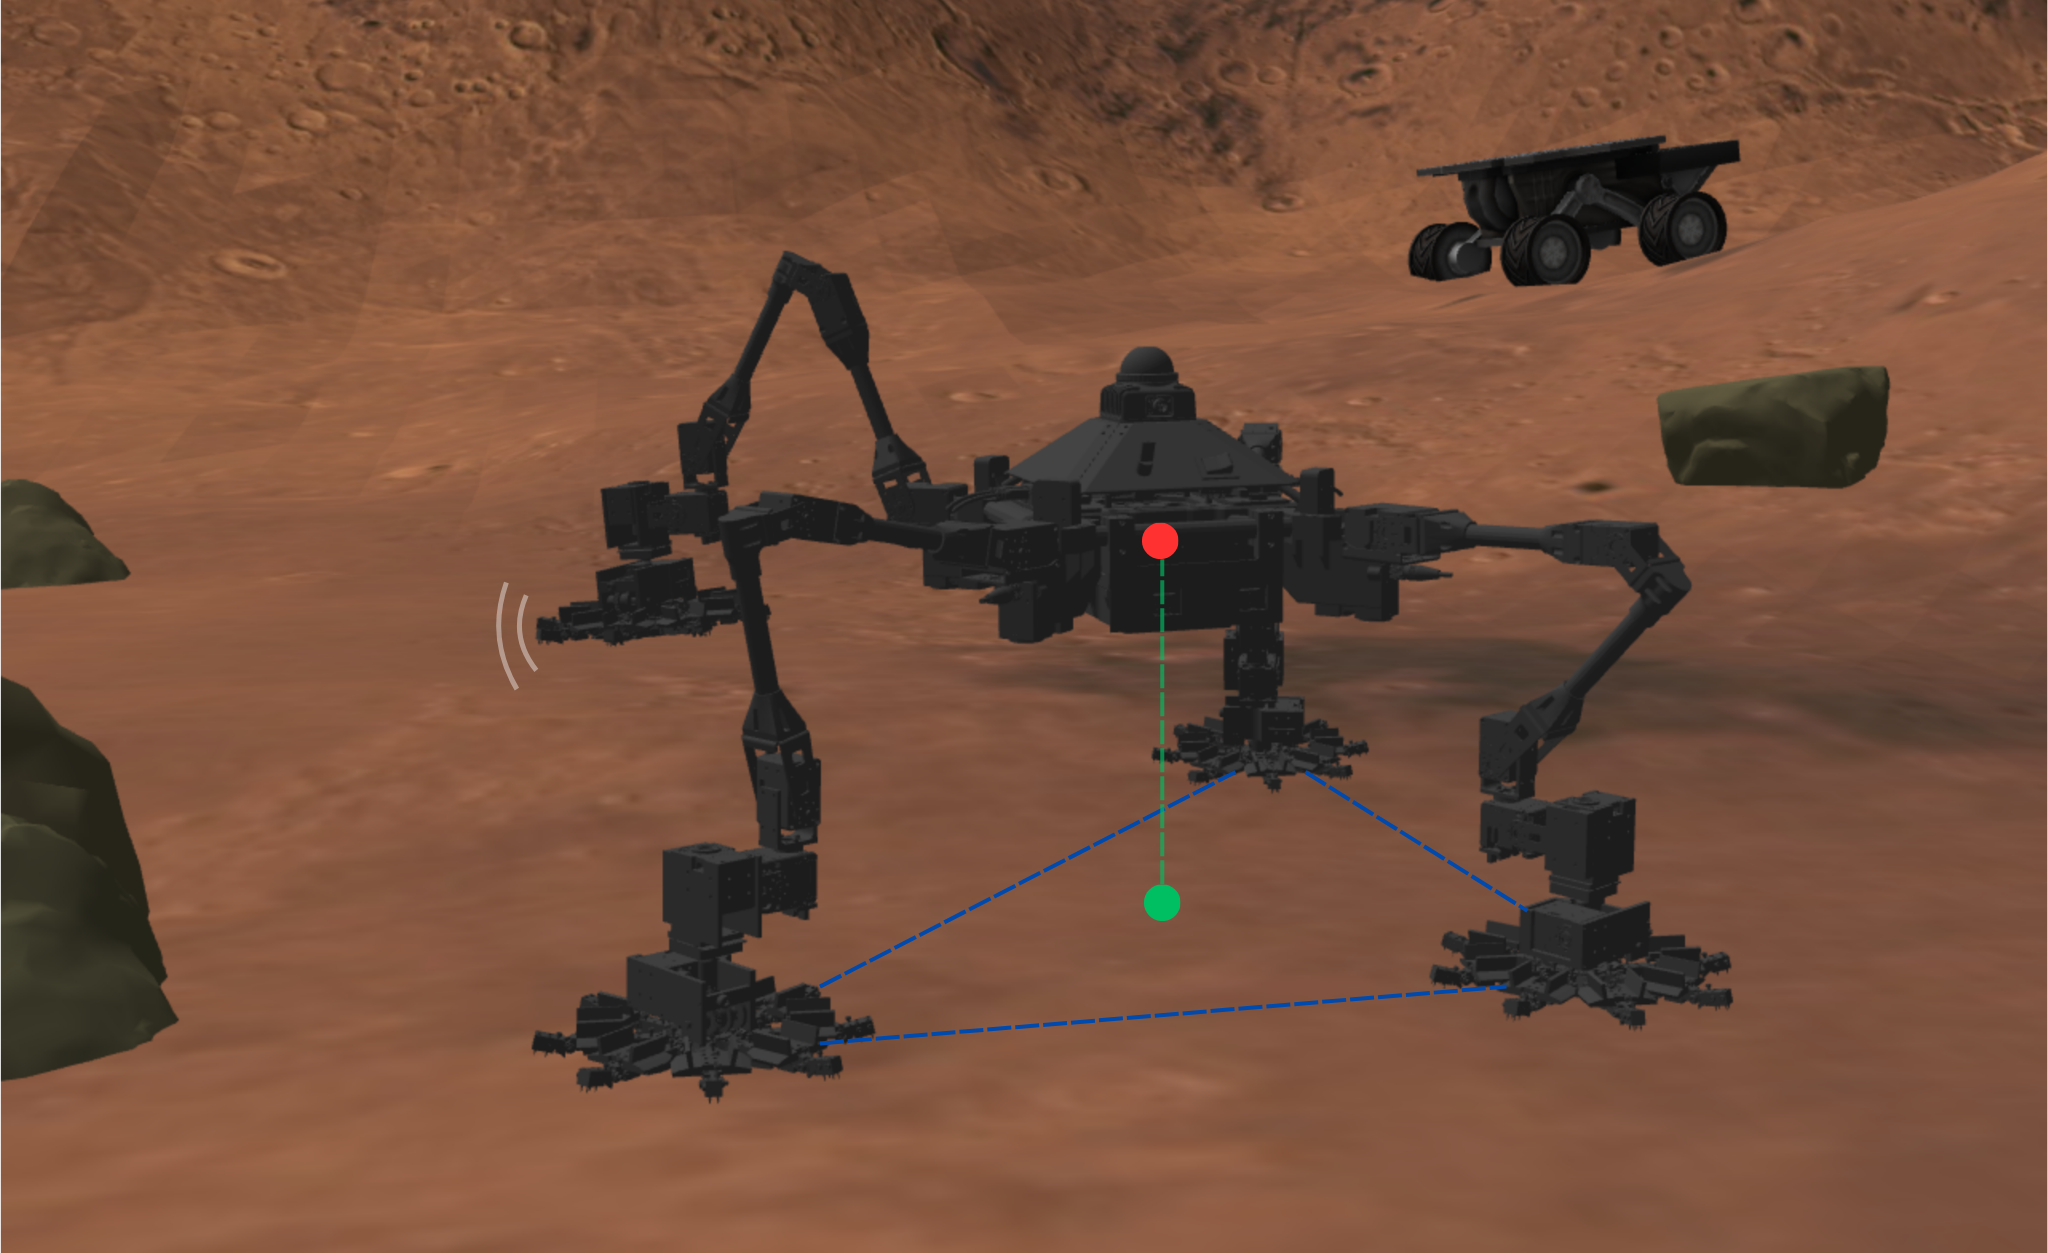
\includegraphics[width=0.5\textwidth]{Images/img_ch5/alg_idea.png}
    \caption{LIMBERO-GRIEEL in a stable configuration ready for single limb transition.}
    \label{fig:limbero_grieel_mars_stable}
\end{figure}
With this approach, the overall mode transformation is decomposed into single-limb problems, and addressing this involves multi-limbed robot stability. 
It is important to note that when GRIEEL goes under a W2G or G2W transition, in both cases ground contact is not admissible, because during the wrist's joints reconfiguration ground sliding may affect the overall structure or damage the module itself. For this reason, any module mode change involves rising up the corresponding limb and maintaining it for the whole transition time. 

For this reason, during a single module transition, LIMBERO-GRIEEL stands on the remaining three limbs, which are responsible for maintaining a stable configuration while the limb is not in contact.

From now on, the algorithm is described for the quadruped robot LIMBERO-GRIEEL used in this research, but some aspects of the extension for N-limbed robots are discussed in the last section. The notation and symbols introduced in the previous chapters are used with the same meaning. 

The type of problem discussed above is a common problem when planning a static gait\cite{McGhee}\cite{Todd}\cite{Raibert}\cite{HiroseDesignGate}, where a stable base CoM positioning is involved during each walking step 
(Dynamic gaits such as trotting\cite{Raibert} are faster but involve an unstable condition during walking locomotion, so they are not considered here).  

The motion sequence to transform limb $j \in J$ can be described at a high level in the following steps: 
\begin{enumerate}
    \setlength\itemsep{-0.7em} 
    \item\label{item:single_1} Select the limb to transform, $j$.  
    \item\label{item:single_2} move the base in a stable configuration for the upcoming limb lift.
    \item\label{item:single_3} lift limb $j$. 
    \item\label{item:single_4} Transform limb $j$ (G2W/W2G).
    \item\label{item:single_5} lay down limb $j$ in the new mode.
\end{enumerate}

The single transition sequence is simple, but step (\ref{item:single_2}) has to be properly defined to give motion commands to the robot, and the "stable base configuration" problem has infinite solutions. If the SSM criterion is used, according to theorem \ref{th:static_stability}, all the feasible configurations where the base CoM projects inside the SP (a continuous space) are fine. 

An approach similar to base positioning for static walking could be used, positioning the base CoM by maximizing the SSM (or an equivalent ZMP margin). This ensures robust stability, but as discussed when introducing the BME (see  chapter\ref{sec:base_manipolability}), it may cause not dexterous configuration, especially for multi-limbed robots that use their body to manipulate objects in the environment.
Another approach also used for gait generation is to ensure a positive SSM, without maximizing it. This gives a lot of freedom, and it is the approach used here and implemented with a simple rule of thumb. 

Multi-limbed robots are young robotic systems, where full autonomy is still under development and research, for this reason, techniques for optimal configurations with a multipurpose view do not exist.\\
A rule of thumb is used here in terms of stability, but it is clear that when LIMBERO-GRIEEL performs a single W2G transition, sample collecting may be the next task, so having the base ready to do it enables better maneuverability and efficiency. This reason gave birth to the BME.

\begin{figure}[H]
    \centering
    \subfloat[$j=LF$, Upcoming support polygon\label{fig:translation1_ex1}]{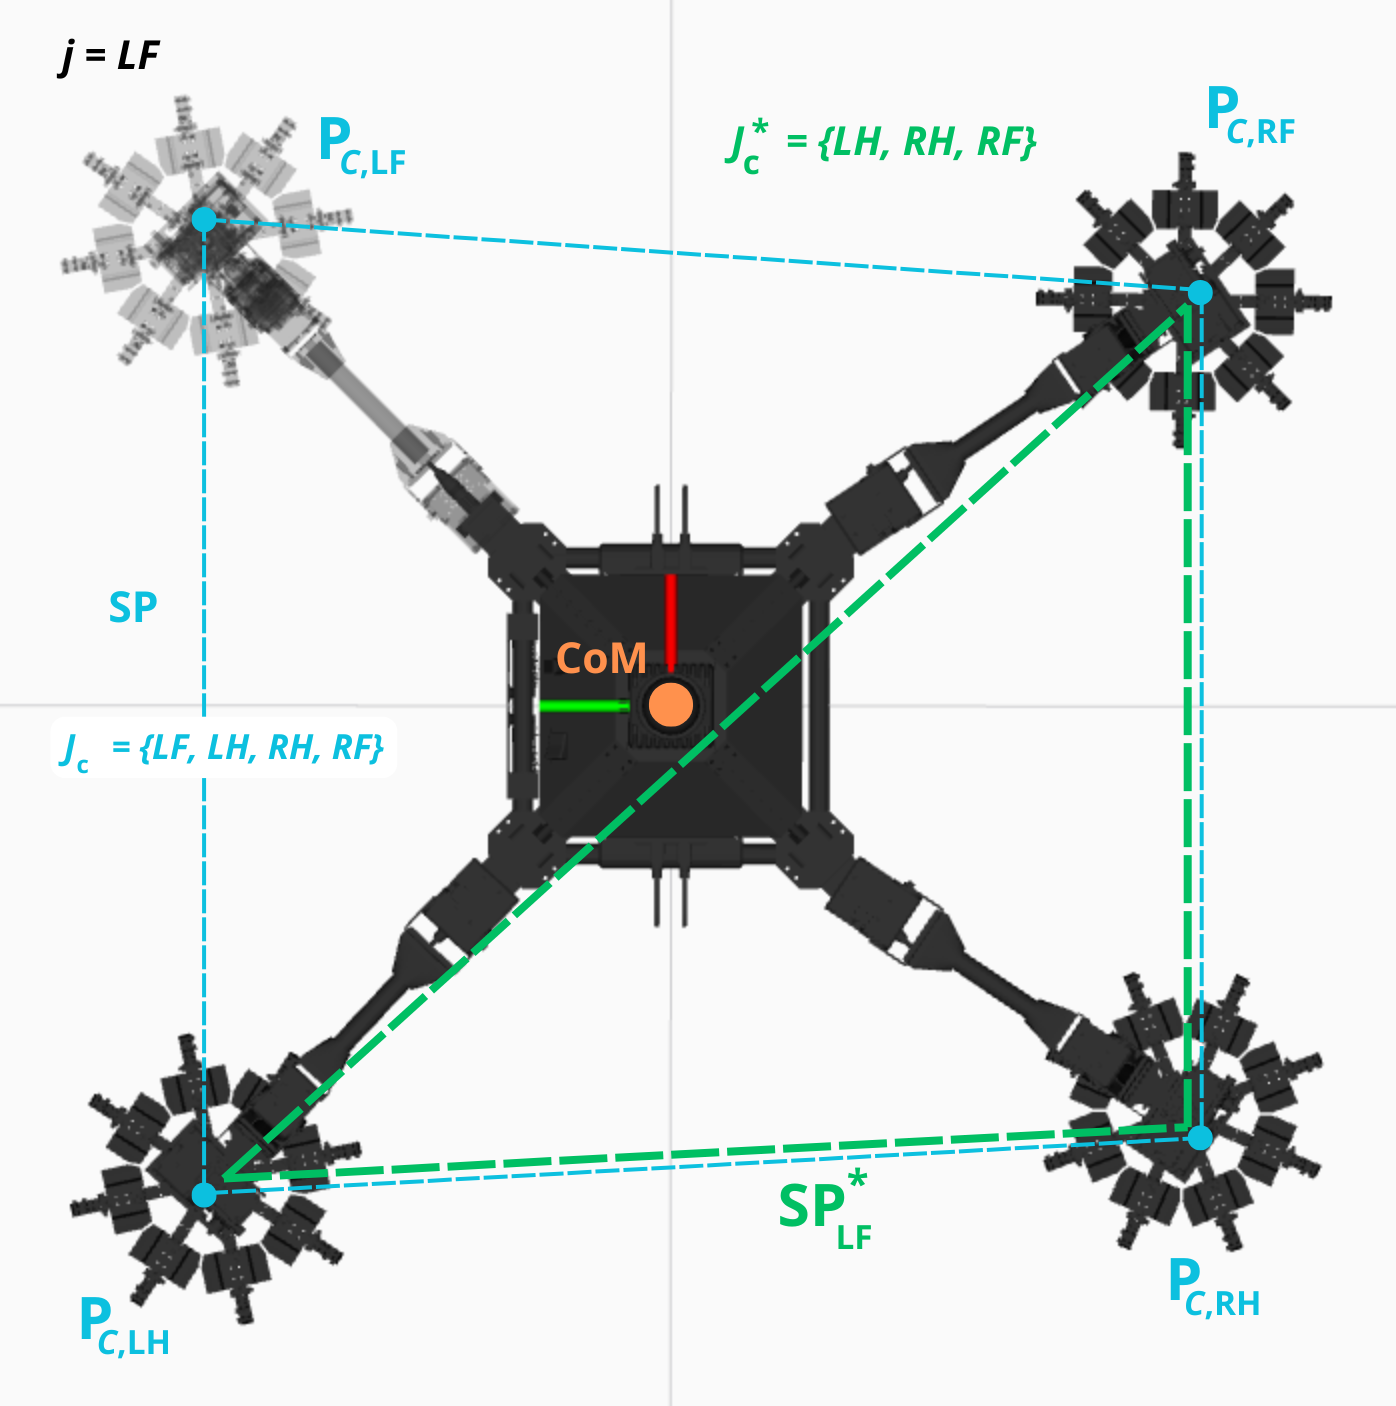
\includegraphics[width=0.3\textwidth]{Images/img_ch5/translation1_ex1.png}} \quad 
    \subfloat[Involved vectors\label{fig:translation2_ex1}]{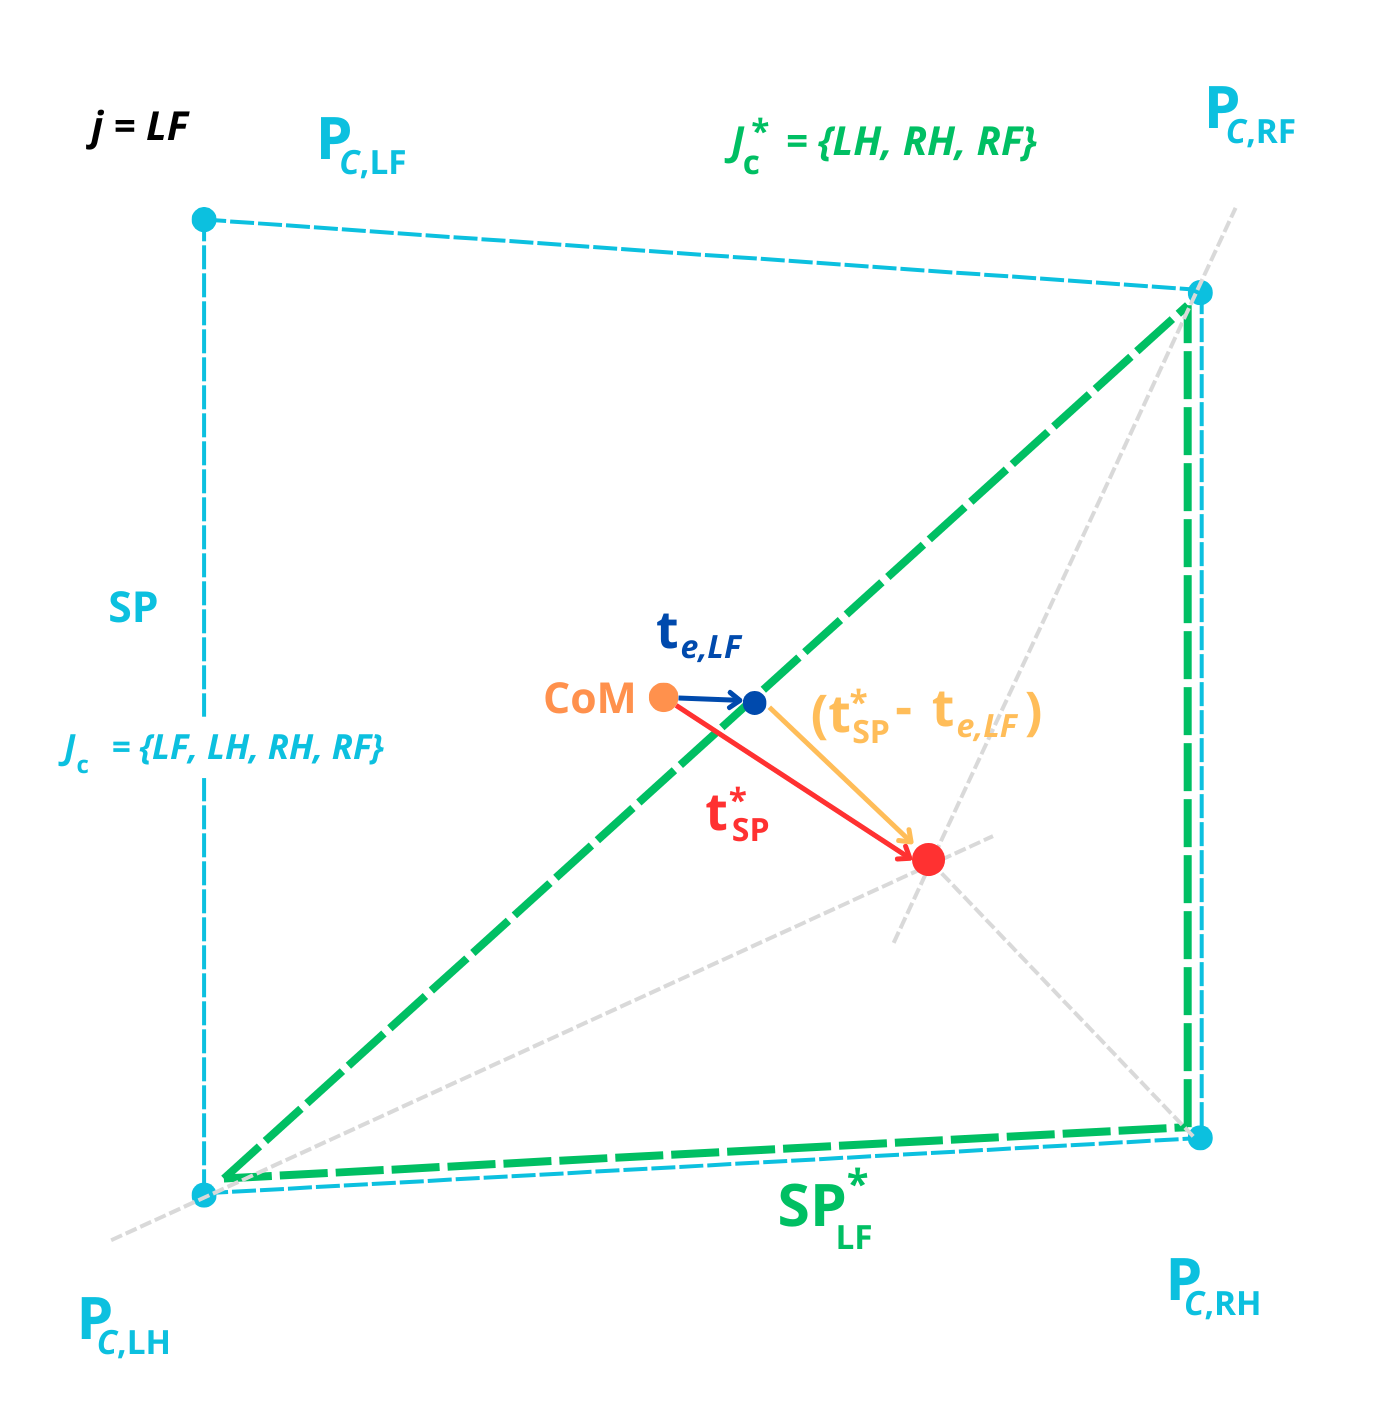
\includegraphics[width=0.3\textwidth]{Images/img_ch5/translation2_ex1.png}} \quad
    \subfloat[Final base translation\label{fig:translation3_ex1}]{\includegraphics[width=0.3\textwidth]{Images/img_ch5/translation3_ex1.png}}   \quad
    \\
    \subfloat[$j=RF$,Upcoming support polygon\label{fig:translation1_ex2}]{\includegraphics[width=0.3\textwidth]{Images/img_ch5/translation1_ex2.png}}\quad
    \subfloat[Involved vectors\label{fig:translation2_ex2}]{\includegraphics[width=0.3\textwidth]{Images/img_ch5/translation2_ex2.png}}\quad
    \subfloat[Final base translation\label{fig:translation3_ex2}]{\includegraphics[width=0.3\textwidth]{Images/img_ch5/translation3_ex2.png}}
    \caption[Schematic representation of base translation rule of thumb]{Schematic representation of base translation rule of thumb}
    \label{fig:base_rule_of_thumb}
\end{figure}

The rule of thumb used to position the base of LIMBERO-GRIEEL is schematized for different SP cases in Fig.\ref{fig:base_rule_of_thumb} above, and can be formalized mathematically. Considering all the vectors measured in a frame attached to $\overline{\mathbf{P}_{CoM}}$, and denoting with $\mathbf{t^*_b}_{,j}$ the required base motion when limb $j$ is the upcoming rising limb, $\mathbf{t^*_{SP}}$ the upcoming SP center, and $\mathbf{t_e}_{,j}$ the midpoint of the edge connecting the adjacent limbs (for example, the adjacent limbs of LF are LH and RF, while RH is the opposite), the base motion is computed as:   
\begin{equation}
    \label{eq:base_motion_rule_of_thumb}
    \mathbf{t^*_b}_{,j} = \mathbf{t_e}_{,j} +  \frac{(\mathbf{t^*_{SP}} - \mathbf{t_e}_{,j})}{3} 
\end{equation}
Simplified to 
\begin{equation}
    \label{eq:base_motion_rule_of_thumb_final}
    \mathbf{t^*_b}_{,j} = \frac{2}{3}\mathbf{t_e}_{,j} + \frac{1}{3}\mathbf{t^*_{SP}} 
\end{equation}

Denoting with $SP_j^*$ the upcoming support pattern ($SP^* \subset SP$) when limb $j$ is raised and all $k\not=j$ limbs' contact points $\mathbf{P}_{c,k}$ fixed, and with $J_c^* = J_c/j$ the upcoming set of contact points. Considering that before the transformation, if all limbs are in contact (included as an initial condition) $J_c = J$, it holds: 
\begin{equation}
    \label{eq:upcoming_SP}
    SP^* = Conv(J_c^*) 
\end{equation}
Where $Conv(\cdot)$ denotes the convex hull as defined in (\ref{eq:SP}).

In Equation \ref{eq:base_motion_rule_of_thumb} the meaning of that base translation is clear:\\
the final base position is such that the CoM will project in a point which is at $\frac{1}{3}$ of the length of the segment between the midpoint of the closest $SP^*$ edge and the center of $SP^*$. \\
So, in any condition, it holds $SSM^* = \frac{1}{3}max(SSM)$.

It is possible to compute $\mathbf{t^*_{SP}}$ and $\mathbf{t_e}_{,j}$ as:
\begin{equation}
    \label{eq:SP_center}
    \mathbf{t^*_{SP}} = \frac{\sum_{k\in J^*_c}\mathbf{P}_{c,k}}{3}
\end{equation}
\begin{equation}
    \label{eq:middle_vec}
    \mathbf{t_e}_{,j} = 
    \begin{cases}
    \frac{\mathbf{P}_{c,LF} + \mathbf{P}_{c,RH} }{2} \quad if \text{ } j\in \{LH,RF\}
    \\
    \frac{\mathbf{P}_{c,RF} + \mathbf{P}_{c,LH} }{2} \quad if \text{ } j \in \{LF,RH\}
    \end{cases}
\end{equation}

The definition of the $SP$ and $SP^*$ is fundamental to understanding the theory, but in principle, to compute the desired base translation, the set of contact points $\mathbf{P_c} = \{\mathbf{P}_{c,j} | j\in J_c\}$ is enough. 

So, based on equations (\ref{eq:base_motion_rule_of_thumb_final})(\ref{eq:SP_center})(\ref{eq:middle_vec}) it is possible to define a primitive procedure, that returns the desired base translation given the set of contact points and the limb to raise:
\begin{equation*}
    \textit{BaseTranslation}^*: (\mathbf{{P}_c}, j) \rightarrow \mathbf{t^*_b}_{,j}
\end{equation*}

Finally, all the elements to define the motion sequence for a single are formalized, and the complete procedure is formalized in  (\ref{alg:single_grieel_transition}), with the proper level of detail.
This computational sequence corresponds to the steps previously defined.
The details on limb height, wrist configuration, and grieel mode are neglected here, but implemented in the final software. A schematic representation of this together with the real system sequence is reported in Fig.\ref{fig:single_limb_transform}.

\begin{algorithm}[H]

    \caption{SingleGRIEEL\_Transformation($\mathbf{P_c}$, $j$)}
    \label{alg:single_grieel_transition}
    \begin{algorithmic}[1]
    \IF{$|\mathbf{P_c}| < 4$}
    \STATE{\textbf{return} FAIL "Not enough limbs in contact"}
    \ENDIF
    \STATE{$\mathbf{t^*_b}_{,j} \leftarrow \textit{BaseTranslation}^*$($\mathbf{P_c}$, $j$)}
    \STATE{Move the base by $\mathbf{t^*_b}_{,j}$ (base motion task)}
    \WHILE{base task \textbf{not} finsh}
    \STATE{check and wait}
    \ENDWHILE
    \STATE{Raise limb $j$ (limb motion task)}
    \WHILE{limb task \textbf{not} finish}
    \STATE{check and wait}
    \ENDWHILE
    \STATE{Send new joint set point $j\_wristH$, $j\_wristV$}
    \STATE{Send new open/closing command (GRIEEL change task)}
    \WHILE{grieel task \textbf{not} finish}
    \STATE{check and wait}
    \ENDWHILE
    \STATE{lay down limb $j$ (limb motion task)}  
    \STATE{\textbf{return} SUCCESS} 
    \end{algorithmic}
\end{algorithm} 


\begin{figure}[H]
    \centering
    \subfloat[Compute base translation\label{fig:single_1}]{\includegraphics[width=0.3\textwidth]{Images/img_ch5/robot_G2W_1.png}} \quad 
    \subfloat[Move the base\label{fig:single_2}]{\includegraphics[width=0.3\textwidth]{Images/img_ch5/robot_G2W_2.png}} \quad
    \subfloat[Raise the limb\label{fig:single_3}]{\includegraphics[width=0.3\textwidth]{Images/img_ch5/robot_G2W_3.png}}   \quad
    \\
    \subfloat[Change wrist joints\label{fig:single_4}]{\includegraphics[width=0.3\textwidth]{Images/img_ch5/robot_G2W_4.png}}\quad
    \subfloat[Transform GRIEEL \label{fig:single_5}]{\includegraphics[width=0.3\textwidth]{Images/img_ch5/robot_G2W_5.png}}\quad
    \subfloat[Lay down the limb\label{fig:single_6}]{\includegraphics[width=0.3\textwidth]{Images/img_ch5/robot_G2W_6.png}}
    \caption[Single limb transition sequence]{Single limb transition sequence}
    \label{fig:single_limb_transform}
\end{figure}

Then, exploiting the procedure defined above, a full locomotion transition is easy to define as a special case of multiple limb transition, where $J^* = J$, with $J^*$ as the ordered set of limbs to transform. Before defining it, an additional primitive procedure that returns the set of contact point positions is needed (on software, managed by state estimators):
\begin{equation*}
    \textit{CheckContact}: () \rightarrow \mathbf{P_c}
\end{equation*}
Finally, all the required elements are defined, the algorithm is reported below, and Fig.\ref{fig:complete_transition} summarizes it with a simple high-level diagram. 

\begin{algorithm}[H]
    \caption{MultipleGRIEEL\_Transformation($\mathbf{P_c}$, $J^*$)}
    \label{alg:multiple_grieel_transition}
    \begin{algorithmic}[1]
    \STATE{$N_{task} \leftarrow |J^*|$}
    \STATE{$first\_limb \leftarrow$ True}
    \STATE{$finish\_transform \leftarrow$ False}
    \IF{$|\mathbf{P_c}| < 4$}
    \STATE{\textbf{return} FAIL "Not enough limbs in contact"}
    \ENDIF
    \FOR{$l = 1,...,N_{task}$}
    \IF{$(first\_limb \textbf{ or } finish\_transform)$}
    \STATE{$\mathbf{P_c} \leftarrow \textit{CheckContact}$}
    \STATE{$\textit{result} \leftarrow SingleGRIEEL\_Transformation$ ($\mathbf{P_c}$, $l$)}
    \IF{$result = SUCCESS$}
        \STATE{$finish\_transform \leftarrow$ True} 
    \ELSE
        \STATE{\textbf{return} FAIL "Error during limb $l$ Transformation"}
    \ENDIF
    \ENDIF
    \ENDFOR
    \STATE{\textbf{return} SUCCESS} 
    \end{algorithmic}
\end{algorithm} 

\begin{figure}[H]
    \centering
    \includegraphics[width=1.1\textwidth]{Images/img_ch5/complete_transition.png}
    \caption{Schematic representation of the transformation algorithm}
    \label{fig:complete_transition}
\end{figure}


\section{Manipulability analysis with ATBVME and SSM}
\label{sec:base_ellipsoid_algorithm}

In the previous section, the autonomous and adaptable transformation algorithm has been formally defined and qualitatively analyzed. From that description, it can be identified as an anticipative planner, computing motion tasks based on the future robot configuration estimation, with the objective of optimizing stability and dexterity. 
The quantification of these performance requirements is now addressed with a kinematic analysis, using the ATBVME for dexterity and the SSM for stability. 

Furthermore, to derive a more general performance measure, a normalized percentage SSM has been defined as: 

\begin{equation}
    \label{eq:base_motion_rule_of_thumb_final}
    SSM_\% = \frac{SSM}{SSM_{max}}\cdot100
\end{equation}

With the SSM defined in Eq.\ref{eq:SSM_2} (considered null if negative), and the $SSM_{max}$ as maximum stability margin when all four limbs touch the ground in the standard walking configuration (reported in Fig.\ref{fig:limbero_walking}). 
This normalized index is useful to compare different multilimbed robotic systems, defining a measure independent from the robot dimension.  

The algorithm has been implemented in MATLAB with the DH kinematic model derived from the URDF description, and the results of some steps of a gripper-to-wheel transformation sequence are reported in Fig.\ref{fig:G2W_analysis_LF} and \ref{fig:G2W_analysis_RF} below. The transition sequence has been tested with $J^* = \{LF, LH, RH, RF\}$. The graphical elements are interpreted as defined in Chapter \ref{sec:ME_multi_limb_example}, with the additional \textbf{Upcoming Support Polygon}, identified by a blue discontinuous line perimeter, and the end effector represented by a red circle (Wheel or Gripper). 

The rule of thumb defined previously ensures a $SSM_{max}$ always above the $15\%$, and an ATBVME with preferred direction of motion parallel to the ground plane, in the base xy plane(cutting the ellipsoid with a plane on the xy plane o the base frame, it is a circle). This dexterity property ensures ease of base translation in the xy plane, and in case of unexpected disturbances, it guarantees a quick and effective response for base stabilization. 

Now, the performance above is compared with the redefined sequence, where the base motion task is computed maximizing the SSM on three contact limbs (moving in the upcoming support center): 
\begin{equation}
    \label{eq:base_motion_rule_centering}
    \mathbf{t^*_b}_{,j} = \mathbf{t^*_{SP}}
\end{equation}

With this redefinition, only stability is considered, and the results are reported in Fig.\ref{fig:G2W_optimal_analysis_LF} and \ref{fig:G2W_optimal_analysis_RF}. The increase in stability is proven by the fact that the $SSM_\%$ is maintained above 45\% during the transition. However, higher base displacements are involved in reaching the configuration with maximum stability.  
Comparing the ATBVME (as in Fig.\ref{fig:base_LF} and Fig.\ref{fig:base_LF_opt}, or Fig.\ref{fig:base_RF} and Fig.\ref{fig:base_RF_opt}), when the base task is computed as in (\ref{eq:base_motion_rule_centering}), the preferred direction of motion has a non-negligible rotation from the xy plane.

As discussed in Chapter\ref{ch:chapter_three}, the direction of the ellipsoid major axis is the relevant information to analyze dexterity, meaning that, the rotated ellipsoid is interpreted as a dexterity loss in the main direction of base stabilization. In conclusion, the rule of thumb is optimal in terms of manipulability, if stability is important, the next support center can be integrated in the transformation sequence.

Finally, the driving configuration after G2W transition is reported in Fig.\ref{fig:Driving_Manipulability}.

\begin{figure}[H]
    \centering
    \subfloat[Next support polygon estimation\label{fig:support_LF}]{\includegraphics[width=0.9\textwidth]{Images/img_ch5/step1_ruleofthumb.png}} 
    \\
    \subfloat[Base motion task\label{fig:base_LF}]{\includegraphics[width=0.9\textwidth]{Images/img_ch5/step2_ruleofthumb.png}} 
    \\
    \subfloat[Raise limb and GRIEEL transformation\label{fig:raise_LF}]{\includegraphics[width=0.9\textwidth]{Images/img_ch5/step3_ruleofthumb.png}} 
    \\
    \subfloat[Limb down\label{fig:down_LF}]{\includegraphics[width=0.9\textwidth]{Images/img_ch5/step4_ruleofthumb.png}} 
    \caption[First limb (LF) transition sequence, rule of thumb]{First limb (LF) transition sequence, with the rule of thumb base motion (perspective, xy, and xz view) }
    \label{fig:G2W_analysis_LF}
\end{figure}

\begin{figure}[H]
    \centering
    \subfloat[Next support polygon estimation\label{fig:support_RF}]{\includegraphics[width=0.9\textwidth]{Images/img_ch5/step5_ruleofthumb.png}} 
    \\
    \subfloat[Base motion task\label{fig:base_RF}]{\includegraphics[width=0.9\textwidth]{Images/img_ch5/step6_ruleofthumb.png}} 
    \\
    \subfloat[Raise limb and GRIEEL transformation\label{fig:raise_RF}]{\includegraphics[width=0.9\textwidth]{Images/img_ch5/step7_ruleofthumb.png}} 
    \\
    \subfloat[Limb down\label{fig:down_RF}]{\includegraphics[width=0.9\textwidth]{Images/img_ch5/step8_ruleofthumb.png}} 
    \caption[Final limb (RF) transition sequence, rule of thumb]{Final limb (RF) transition sequence, with the rule of thumb base motion (perspective, xy, and xz view)}
    \label{fig:G2W_analysis_RF}
\end{figure}


\begin{figure}[H]
    \centering
    \subfloat[Base motion task\label{fig:base_LF_opt}]{\includegraphics[width=0.9\textwidth]{Images/img_ch5/step2_centering.png}} 
    \\
    \subfloat[Raise limb and GRIEEL transformation\label{fig:raise_LF_opt}]{\includegraphics[width=0.9\textwidth]{Images/img_ch5/step3_centering.png}} 
    \\
    \subfloat[Limb down\label{fig:down_LF_opt}]{\includegraphics[width=0.9\textwidth]{Images/img_ch5/step4_centering.png}} 
    \caption[First limb (LF) transition sequence, base centering]{First limb (LF) transition sequence, with base centering (perspective, xy, and xz view)}
    \label{fig:G2W_optimal_analysis_LF}
\end{figure}

\begin{figure}[H]
    \centering
    \subfloat[Next support polygon estimation\label{fig:support_RF_opt}]{\includegraphics[width=0.9\textwidth]{Images/img_ch5/step5_centering.png}} 
    \\
    \subfloat[Base motion task\label{fig:base_RF_opt}]{\includegraphics[width=0.9\textwidth]{Images/img_ch5/step6_centering.png}} 
    \\
    \subfloat[Raise limb and GRIEEL transformation\label{fig:raise_RF_opt}]{\includegraphics[width=0.9\textwidth]{Images/img_ch5/step7_centering.png}} 
    \\
    \subfloat[Limb down\label{fig:down_RF_opt}]{\includegraphics[width=0.9\textwidth]{Images/img_ch5/step8_centering.png}} 
    \caption[Final limb (RF)transition sequence, base centering]{Final limb (RF) transition sequence, with base centering (perspective, xy, and xz view)}
    \label{fig:G2W_optimal_analysis_RF}
\end{figure}

\begin{figure}[H]
    \centering
    \includegraphics[width=0.9\textwidth]{Images/img_ch5/driving.png}
    \caption{SSM and ATBVME in driving configuration  after G2W transition (perspective, xy, and xz view)}
    \label{fig:Driving_Manipulability}
\end{figure}


\section{Final comments on the Proposed Algorithm}
\label{sec:comments}
In this chapter, a versatile and reliable algorithm to perform the transition of one, multiple, or all modules of LIMBERO-GRIEEL has been defined.
Now some of the comments previously anticipated are discussed, starting from a detailed comparison between the previous and the proposed algorithm


\subsection{Algorithms Comparison}
\label{sec:comparison}

The new algorithm's advantages have additional costs in terms of energy and time required.
The new motion sequence for each module transformation involves one base task (stabilize), two limb tasks (raise and lay down), and one GRIEEL change task (transform). Hence, if a complete locomotion transition is needed, the number of motion tasks involved is higher than that of the previous algorithm. On the other hand, single-limb transitions are faster and less demanding. 
Furthermore, the base motion tasks have been defined to be reliable in the sense of stability, and dexterous in the sense of not wasting motion and maintaining maneuverability, which can reduce the required time and the power consumed. 

Additional experiments and measurements should be done for a quantitative comparison of the two methods in terms of energy consumption. Laying down the base and raising it involves all limb motion, meaning that this qualitative analysis may be wrong. 

 In addition to time and energy considerations, it is important to notice that under some conditions which have been discussed in detail, the old algorithm may cause system failure or damage, in those cases, the proposed one is the clear choice.  

There is no "best" solution for all the conditions, it depends on the environment, the mission requirements, and the available resources. 
Exteroceptive and proprioceptive sensors and mission requirements can be used to infer the optimal choice, enabling multiple transition algorithms instead of prescribing only one possibility.

\subsection{Extensions}
\label{sec:extensions}

Section \ref{sec:new_algorithm} describes the transition sequence for a quadruped robot, moving in an environment where SP criteria and SSM are enough to ensure stability (flat and almost horizontal).

In the algorithm definition, the current locomotion capabilities have been considered, where the robot can walk, climb, or drive with the configurations described in (\ref{sec:locomotion_configurations}). The complex mechanical structure and redundancy of L-G's limbs allow complex locomotion capabilities, and it is interesting to analyze the possible future extensions of the transition algorithm. 

The transformation extensions are briefly discussed for the following cases: working in different terrain conditions, taking advantage of dynamic mode transition or in advanced configurations, and having more than 4 limbs.  

\subsubsection{Different Terrain Conditions}
\label{sec:different_conditions}

In most cases, the assumption of flat and almost horizontal terrain when mode transition occurs can be met, or even imposed, and it is possible to give an intuitive explanation of this. 
When a full locomotion transition occurs, these two cases are the most common: 
\begin{itemize}
    \setlength\itemsep{-0.7em} 
    \item \textbf{Walking to driving}: Locomotion mode transition is considered when moving from a rough terrain to a regular one. This transformation occurs when the terrain changes into a drivable condition, so terrain regularity and negligible slopes are needed. In those conditions, the transformation command is sent when the drivable ground is reached, where SSM is a reliable criterion.   
    \item \textbf{Driving to walking}: When the opposite occurs and motion from drivable to uneven terrain occurs, the transition W2G is enforced before entering the walking zone. 
\end{itemize}

If advanced locomotion and adaptive usage of limbs are considered, the following cases can extend the  transformation scenarios: 
\begin{itemize}
\setlength\itemsep{-0.7em} 
    \item \textbf{Driving on Slopes}: If satisfactory driving performances are met in wheel mode, in terms of traction and reduced slippage, driving on slopes is possible. In those sloped driving cases, the terrain is considered almost flat but not horizontal, then the SSM is not reliable, and the ZMP has to be considered.   
    \item \textbf{Driving exploiting limbs}: Furthermore, if complex limb configurations are considered and adapted to the terrain during driving, the flat ground constraint of wheeled locomotion is no longer necessary\cite{AnymalDocThesis}\cite{MAMMOTH}\cite{WheelLeggedStabilityOPT}. 
    \item \textbf{Dynamic transformation}: As discussed in the next section, complex robot configuration may occur during the transition when the full system's potential is exploited. 
    The terrain can be irregular, the inertial effect non-negligible, and the gripping forces relevant. 
\end{itemize} 

In those scenarios, the SSM is unreliable (as discussed in chapter \ref{ch:chapter_three}), and more advanced stability criteria like the ZMP, TSM, or GIA are better choices. 

Thanks to the modularity of the proposed transition algorithm, integrating different stability criteria is possible. After classifying the terrain condition and the contact points/forces, the base translation is defined accordingly, and stability can be ensured. 

\subsubsection{Hybrid locomotion and Dynamic Transition}
\label{sec:different_conditions}

Understanding what is and when hybrid locomotion is possible serves the purpose of introducing another possible condition where module transition may be exploited. 

Previously the term "hybrid configuration" has been used to indicate a configuration in which the robot has different types of EE during task execution. \textit{Hybrid locomotion} instead, indicates the type of locomotion where an EE built for a specific function is used differently. An example is walking with wheeled limbs (locking the driving joints in the meantime), and researchers at ETH proved with ANYmal on wheels\cite{AnymalDocThesis}that this is possible and enables new capabilities. 

While a multi-limbed robot with GRIEEL can transform the locomotion module, in most conventional robots either wheels or gripper/foot are mounted. The considerations of the different locomotion efficiency (behind the development of GRIEEL) explain why walking locomotion with wheeled legs has been studied \cite{AnymalDocThesis}\cite{WheelLegged}.

The main problem with wheeled walking locomotion is that some terrains are completely unfeasible to walk in using a wheel-shaped foot. In those contexts, GRIEEL multimodality surpasses every other system.
However, implementing a possible walking wheeled gait with GRIEEL can further increase the potentiality of the system, for example: 
\begin{itemize}
    \setlength\itemsep{-0.7em} 
    \item \textbf{Obstacles when driving while manipulating}: When LIMBERO-GRIEEL (or any quadruped limbed-robot using GRIEEL) is in a hybrid configuration, on three wheels and the last limb carrying an object, the global path to the goal location has to be planned considering only driving locomotion. If a locomotion transition is needed on a small portion of the path, and the base cannot be supported on the ground, the object has to be temporarily dropped to ensure three points of contact during limb transformation. If instead, the roughness of the terrain is such that walking wheeled can be considered in those critical points, mission time and effort are significantly reduced. 
    \item \textbf{Few obstacles on the driving path}: In conditions similar to the one listed above, where wheeled locomotion is feasible along the path, except for a small portion. When that portion allows hybrid locomotion, maintaining wheel mode is probably the most efficient solution.   
\end{itemize}

Those considerations require complex path planning and decision-making, based on terrain traversability analysis, global cost maps, and representative cost functions. The description of such algorithms and procedures is above the scope of this research, but it is a required capability to enable system autonomy to exploit its full potential.  

Considering also hybrid locomotion, it is possible to extend the possible module transition to dynamic conditions: 
\begin{itemize}
    \setlength\itemsep{-0.7em} 
    \item \textbf{Transition during locomotion}: In case the transition occurs during a path-following task, the transition sequence has been defined as a pause on the path execution. It is possible to redefine that single module transformation (\ref{alg:single_grieel_transition}) as part of a limb trajectory during a walking step. With this approach, when a full locomotion transition is needed, additional steps toward the final location can be completed during mode transformation.  \item \textbf{Hybrid locomotion recovery}: When hybrid locomotion is in execution, but criticality occurs because of inaccurate planning, a transition to gripper mode has to start
    \item  \textbf{Driving to climbing}: If a transition from driving to climbing locomotion is imminent, it is possible to perform motions to start climbing during transformation. For example, the front limbs are positioned closer to the climbing wall, and during W2G the grippers are directly attached to the wall instead of laying it back on the ground. 
\end{itemize}

The advanced tasks and possibilities described above are interesting aspects, which require a complex and adaptable control system. 
However,  in terms of the module transition, the reusability of the single transformation can be exploited, defining additional components that account for adaptable limb and base tasks. 

\subsubsection{N-limbed Robots}
\label{sec:N_limbed_extension}

GRIEEL has been tested and analyzed as an extension of LIMBERO's limbs, however, its final purpose is to become a reusable module to be integrated into different limbed robots. The mechanical design is already independent of the limb, but additional efforts will be necessary to make its control software modular and reusable.

The details on this reusability design requirements are out of this research scope. It is interesting to analyze the additional considerations and functionalities the transition algorithm should integrate when GRIEEL is attached to a robot with more than 4 limbs. 

Legged robots are commonly designed with an even number of legs (bipeds, quadrupeds, hexapods,\dots), because of symmetry and periodic gait scheduling. 
Having a transformable module enables additional functionalities, for example, a quadruped limbed robot with GRIEEL as EE can mount a supplemental lighter limb, this can be retracted above the body if properly designed, and extracted for object manipulation or additional driving/walking support in critical conditions. 

In a six-limbed robot (such as SCAR-E \cite{SCAR-E}), by attaching GRIEEL as EE it is possible to exploit the additional stability of more contact points (bigger SP) for manipulation tasks. 
The hybrid configuration previously discussed for L-G here is even more functional, four limbs can be used in driving mode, and two adjacent limbs in gripper mode, enabling cooperative manipulation with two "arm-like" limbs \cite{CooperativeManipulators}. 
Additionally, having 6 wheels provides higher traction force, with the possibility of driving in steeper terrains. 

In terms of the GRIEEL transition algorithm, it is clear that having six possible points of contact makes the single-limb transition much easier. The case of 6-wheeled to 4-wheeled + 2-gripper is easily managed by keeping the 4-wheeled limbs on the ground and raising the ones to transform (taking into consideration inertial and gravitational effects if affecting the system stability, for example when quick motions are involved or when the limbs are heavy). 

Fig.\ref{fig:sixlimbsGRIEEL} represent conceptually different configurations and functionalities for a robot with six limbs equipped with GRIEEL.


\begin{figure}[H]
    \centering
    \subfloat[hexapod LIMBERO-GRIEEL in Gazebo mars world .\label{fig:hexapod_mars}]{\includegraphics[width=0.7\textwidth]{Images/img_ch5/hexapod_mars.png}} \quad 
    \\
    \subfloat[Gripper mode\label{fig:hexapod_gripper}]{\includegraphics[width=0.38\textwidth]{Images/img_ch5/hexapod_gripper.png}}\quad
    \subfloat[Wheel mode\label{fig:hexapod_wheeled}]{\includegraphics[width=0.38\textwidth]{Images/img_ch5/hexapod_wheeled.png}}\quad
    \\
     \subfloat[Hybrid cooperative frontal  grippers\label{fig:hexapod_manipulate}]{\includegraphics[width=0.38\textwidth]{Images/img_ch5/hexapod_manipulate.png}}\quad
    \subfloat[Hybrid side grippers\label{fig:hexapod_manipulate_side}]{\includegraphics[width=0.38\textwidth]{Images/img_ch5/hexapod_manipulate_side.png}}\quad   
    \caption[Conceptual representation of hexapod LIMBERO-GRIEEL]{Hexapod LIMBERO-GRIEEL in different configurations}
    \label{fig:sixlimbsGRIEEL}
\end{figure}

\BlankPageTLGWfour

\chapter{ LIMBERO-GRIEEL, Controller Tuning}
\label{ch:chapter_six}

This chapter discusses the last step in setting up simulations and experiments on LIMBERO-GRIEEL. 
In chapter \ref{ch:chapter_four} the software infrastructure to control robot motion has been described, but details on the joint controllers' infrastructure have been skipped on purpose.

For different simulation environments and real hardware different configurations and types of controllers have been tested, so it is relevant to discuss it in detail.

First, the system-controller combinations analyzed are summarized, Then for each combination, the controller tuning procedure is explained.

\section{Summary of System-Controller Combinations}
\label{sec:system_controller}

The reason why during this research different set-ups have been used has been clarified in the research workflow (see Section \ref{sec:approach}).In addition, the importance of simulators in testing control architecture and high-level algorithms before any hardware experiments has been discussed in the simulator description \ref{sec:simulation_description}.

Now, the different system-controller setups are summarized. 
In this context, the term "system" refers to the robot as a dynamic mechanical system, while "controller" indicates the low-level component responsible for the joint control. so the controller is the strategy used to compute the control signal from the desired joint position.

The high/middle-level components (all the ROS2 software nodes except the JTC, DYCs, or IJCs) are not discussed here, since they remain the same in all the testing settings. 

The combinations can be summarized as follows: 
\begin{itemize}
    \setlength\itemsep{-0.7em} 
    \item \textbf{Gazebo Classic + JTC}: This is the set-up used at the SRL as the testing environment to implement and integrate the architecture responsible for controlling GRIEEL joints. In this case, the system is the robot URDF model, used by Gazebo Classic to simulate the dynamic system. The controller instead, is an independent joint controller, where each joint command is the joint torque, computed with a closed-loop PID control law from the joint position error. The computations of this controller are handled by ros2\_control.
    Gazebo Classic is not very stable, and the GRIEEL module transition was not possible. 
    
    \item \textbf{LIMBERO-GRIEEL + DYCs}: 
    Because the interface between ros2\_control and DYNAMIXELs motor was not ready during hardware experiments, the desired joint positions were sent directly to the servomotors. The system here is the real robot, while the controller is again an independent joint controller, this time implemented by the internal logic of the DYNAMIXEL servomotor.  

    \item \textbf{MATLAB-Simulink + IJCs}:
    For a model-based controller design and tuning, an approximated dynamic model is identified in MATLAB (the "system"). MATLAB is used because it provides better tools for system identification. Here the terms of the EoM are identified, and a closed-loop independent joint controller is designed with additional blocks such as filters and anti-wind up. 
    
    \item \textbf{Gazebo Harmonic + IJCs}:
    Without the real hardware available, the complete simulation environment is settled up in the more reliable Gazebo Harmonic simulator. The IJCs designed and tuned in MATLAB-Simulink are then implemented as nodes in the ros2 infrastructure, replacing the JTC. Additionally, GRIEEL finger joints are modeled and controlled to simulate a module transition.  
\end{itemize}
A summary of these combinations has been previously represented in Fig.\ref{fig:ros2_simple_scheme}

In all those cases, the joint controller used is based on the limbed-robot IKJC, as already commented in chapter \ref{sec:software_ros2}, and defined in chapter \ref{sec:leggedControl}.
Here the focus is on the relationship between joint position and the controller's action ( joint torque), irrespective of how the set points are computed. 

\section{ros2\_control, Joint Trajectory Controller}
\label{sec:ros2_control}

ros2\_control is a framework for real-time control of robots using ROS2, widely-used control theory implementations (e.g. PID). 
The joint\_trajectory\_controller (JTC) execute joint-space trajectories on a group of joints, 
mapping position + velocity trajectory to effort commands through a PID loop.

The JTC constitutes the low-level motion controller of L-G in Gazebo Classic, which is configured and tuned with an iterative tuning approach.  
The high reduction ratios of the joint motors (as reported in Tab.\ref{table:DYNAMIXEL}), justify a decoupling of the complex mechanical system (as explained in \ref{sec:DecoupledDyn}). For this reason, each joint PID gain can be tuned independently. 

Recalling the notation $q_{j,i}$, which denotes joint $i$ of limb $j$, denoting with $K_{j}$ the set of PID gains for limb $j$, $K_{j} = \{k_{(j,1)}, k_{(j,2)}, k_{(j,3)}, \dots, k_{(j,n_j)} \}$, where $k_{(j,i)} = \{ k_{P,(j,i)}, k_{I,(j,i)}, k_{D, (j,i)}\}$ are the PID gains, and enforcing the condition $n_j = n_h , \forall h\in J /j$ (same number of joints in each limb), the limbs tuning condition is: \\
$K_{h} = K_{j} \quad\ \forall h \in J/j$\\
This condition means that each limb has the same set of gains, and it is related to the symmetry of the mechanical system which requires a symmetric control of limbs. 

From now on, the $j$ index is implicit, because of the condition above.
In principle, the independent tuning approach doesn't impose a specific order, and each joint ($q_i$) controller can be tuned as a SISO system. 
However, to take into account the possible coupling effects neglected with this approach, an iterative adjusting idea is considered, denoted here as \textit{root2end-end2root}.

This idea is based on the classical approach used for empirical PID tuning, once the requirements in terms of settling time, oscillations, over(under)shoot, and steady-state error for each joint are defined, the following tuning steps are conducted: 
\begin{enumerate}
    \setlength\itemsep{-0.7em} 
    \item \textbf{gains initialization}:\\
    Initialize the gains as proportional control, with a meaningful value of $k$ ($k_{P,i} = k, k_{I,i} = 0, k_{D,i}=0 \quad i=1,...,n$ 
    \item \textbf{root2end}: \\
    Start from the limb root joint and proceed towards the serial link chain.\\
    $i = 1\rightarrow2\rightarrow\dots\rightarrow n$ ($i = B2C\rightarrow C2F\rightarrow\dots\rightarrow driving$)
    \begin{enumerate}
        \setlength\itemsep{-0.7em} 
        \item[1.1] Initialize $i=1$
        \item[1.2] Adjust $k_{P,i}$ until satisfied with the settling time 
        \item[1.3] Adjust $k_{D,i}$ to reduce oscillations and over(under)shoots
        \item[1.4] Adjust $k_{I,i}$ to reduce steady-state error
        \item[1.5] Iterate (1.2)-(1.4) until satisfied
        \item[1.6] Until $i < n$, $i = i+1$ and repeat from (1.2)
    \end{enumerate}
    \item \textbf{end2root}: \\
    Adjust the gains of the previous phase from the final serial link joint towards the root.\\
    $i = n\rightarrow n-1\rightarrow\dots\rightarrow 1$ ($i = driving\rightarrow wristV\rightarrow\dots\rightarrow B2C$)
    \begin{enumerate}
        \setlength\itemsep{-0.7em} 
        \item[2.1] Initialize $i=n$
        \item[2.2] Proceed as in (1.2)-(1.5), Adjusting the gains obtained in the root2end phase\\
        \dots
        \item[2.6] Until $i > 1$, $i = i-1$ and repeat from (2.2)
    \end{enumerate}
\end{enumerate}

To analyze the performance of the controllers and compare different tuning, a complete sequence of base and limb motion tasks is performed, and joint state tracking is recorded. 
First, simple motions of the base, and limbs up/down tasks are considered, then the full sequence of motion as defined in the transformation algorithm is evaluated. Tuning in these complex coupled motions ensures the robustness of the controllers. Joints tracking performance for this simulation setup are reported in the results (see Chapter \ref{ch:chapter_eigth}).

\section{DYNAMIXEL Motors}
\label{sec:dynamixel_motors}

When working with the hardware, the joints are controlled with DYNAMIXEL servomotors, those motors accept as input the reference joint position (velocity) and use a common control scheme of DC motors \cite{Siciliano}, with a cascade of position PID (velocity PI) (accordingly to the "control mode" as reported in Tab.\ref{table:DYNAMIXEL}), with additional reference smoothing, rate limiters, and anti-wind up. Furthermore, an internal current control and other controller logic are integrated to improve performance and safety. The control scheme for position (velocity) control is reported in Fig.\ref{fig:dynamixel_control}.
The software interface of the servomotors allows for the change of position (velocity) gains, while the current controller is not accessible. 
\begin{figure}[H]
    \centering
    \subfloat[Position controller in Position Control Mode\label{fig:}]{\includegraphics[width=0.6\textwidth]{Images/img_ch6/position_controller.jpg}} \quad 
    \subfloat[Velocity controller in Velocity Control Mode\label{fig:}]{\includegraphics[width=0.6\textwidth]{Images/img_ch6/velocity_controller.jpg}}  
    \caption[Block scheme of DYNAMIXEL's position and velocity control mode]{Block scheme of DYNAMIXEL's position and velocity control mode}
    \label{fig:dynamixel_control}
\end{figure}

The DYNAMIXEL's closed loop controllers substitute the JTC in achieving the desired motion of the limbs, receiving the same command that was used in the simulation. 

In the transition from simulation to real system, controller gains adjustments are necessary, due to unexpected disturbances and mismatches in the estimated dissipative terms (friction and dumping of the joints).
For this reason, PID gains have been adapted, using again the \textit{root2end-end2root} approach, starting from a gain initialization equal to the values used for the JTC. 

Those modifications have been conducted during the single-limb testing, performed to test and validate the software update to control GRIEEL joints (discussed in the next chapter (\ref{sec:single_limb})).
The interface used to tune DYNAMIXEL controllers is represented in Fig.\ref{fig:dynamixel_GUI}, while the tracking performances after the tuning are reported in Fig.\ref{fig:dynamixel_tracking}.
By default, only proportional control is used, with a quick response but non-negligible steady-state error and overshoots, with the proposed gains instead, the steady-state error is eliminated and overshoots reduced.  

\begin{figure}[H]
    \centering  \includegraphics[width=0.85\textwidth]{Images/img_ch6/DynamixelUI.png}
    \caption{Dynamixel Wizard user interface, a tool to manage DYNAMIXEL motors.}
    \label{fig:dynamixel_GUI}
\end{figure}

Furthermore, when the four limbs were assembled with LIMBERO-GRIEEL, additional couplings between the limbs required small gains corrections.
The final tracking performances of the whole robot, achieved during the transformation, sequence are presented and discussed as part of the conclusions in chapter \ref{ch:chapter_eigth}.

\begin{figure}[H]
    \centering
    \subfloat{\includegraphics[width=0.5\textwidth]{Images/img_ch6/B2C_dynamixel.png}} \subfloat{\includegraphics[width=0.5\textwidth]{Images/img_ch6/C2F_dynamixel.png}} \\
    \subfloat{\includegraphics[width=0.5\textwidth]{Images/img_ch6/F2T_dynamixel.png}} 
\subfloat{\includegraphics[width=0.5\textwidth]{Images/img_ch6/T2E_dynamixel.png}}  \\
    \subfloat{\includegraphics[width=0.5\textwidth]{Images/img_ch6/wristH_dynamixel.png}}  
    \subfloat{\includegraphics[width=0.5\textwidth]{Images/img_ch6/wristV_dynamixel.png}}  \\
    \caption[DYNAMIXELs joint trajectory tracking performance]{DYNAMIXELs joint trajectory tracking performance}
    \label{fig:dynamixel_tracking}
\end{figure}


\section{Indipendent Joint Controller}
\label{sec:IJC}

In the last phase of this research, without access to the hardware, it was necessary to set up a more reliable simulation environment where the transformation of the GRIEEL mechanism could be simulated. As discussed in section \ref{sec:simulation_description}, the choice has been a migration to the newer gazebo version. 
In this simulation environment, it has been possible to expose all joint torque signals and substitute the JTC with closed-loop independent joint controllers (IJCs), implemented from scratch. The new control scheme of each joint is represented in Fig.\ref{fig:IJC_scheme}, it uses a P+PI scheme as the one described in section \ref{sec:IndipendentJointControl}, with an additional reference pre-filter, and anti-wind up based on the back-calculation algorithm\cite{AntiWindUpBackCalculation1}\cite{AntiWindUpBackCalculation2}\cite{AntiWindUpBackCalculation3}\cite{AntiWindUpBackCalculation4}.
Furthermore, in the design of the independent joint controller for the driving motor, a switching controller gains is considered for the driving motor, which is controlled directly at velocity level with a PI controller. For this research, when in gripper mode, the driving motor is kept fixed by the transmission system and the servomotor internal controller, and the proportional and integral gain is set to 0 with a re-initialization of the integrator value. When transforming into wheel mode, instead,  the gains are set to a non-null value (and the integrator is re-initialized)( to control driving locomotion. 

\begin{figure}[H]
    \centering
    \includegraphics[width=0.95\textwidth]{Images/img_ch6/IJC_limbero.png}
    \caption{Block scheme of each joint's IJC, integrated into ROS2 architecture by discretization.}
    \label{fig:IJC_scheme}
\end{figure}

In this new environment, the tuning has been conducted on a single LIMBERO-GRIEEL limb, with a model-based approach instead of an empirical one. As introduced in section \ref{sec:matlab}, the model identification has been carried out in MATLAB. 

The final model is a decoupled joint dynamic, such as the one in \ref{sec:DecoupledDyn}, described by Equation \ref{eq:DecoupledManipulatorEoM}.
However, to take into account the dual nature of the limbs, both a swing and contact model have been defined, considering that when the limb touches the ground it "manipulates" the base (remember the multi-limbed duality with cooperative arms \ref{sec:multi_limb_coopmanipulators}), while if not in contact behave as a robot arm. With this dual, the decoupled dynamic inertia is considered an average of the two models, ensuring more reliability rather than modeling only a swing phase.

The steps of the model identification procedure are summarized here: 
\begin{enumerate}
    \setlength\itemsep{-0.7em} 
    \item Convert the limb simulation model (URDF) to a serial link DH model, referred to as \textbf{limb-DH}, through the required frame transformations. 
    \item Transform dynamic properties (inertia tensor and CoM) of the URDF in the new DH frames
    \item Define the dual model when in contact, by inverting the joint sequence, and considering the robot base as the "tool". 
    \item Identify each joint average inertia from the inertia matrix of the two models, considered in multiple feasible limb configurations.
    \item Derive the equivalent decoupled joint models for all limb joints, referred to as \textbf{limb-IJs}. Where reduction ratio and motor inertia are taken from the online data sheet of DYNAMIXELs. 
\end{enumerate}

From the steps above, both a complete limb model for simulation  (\textbf{limb-DH}) and decoupled joint models (\textbf{limb-IJs}) are available in Matlab.
Finally, limb-IJs are used for controller tuning, while limb-DH for testing the performance of the controllers in a more realistic dynamical system. 

Using the limb-IJs model, classical control theory approaches such as loop shaping are used to derive the gains of the P+PI controllers, ensuring the requirements defined in terms of position/velocity cut-off frequency \cite{ControlTheory}. 
Then limb-DH is imported in a Simulink scheme with a trajectory generator and the implementation of the IJCs, and possible gains correction are considered. 
Furthermore, when porting the controller implementation in ROS2 using Gazebo Harmonic, additional adjustments of those gains are necessary to counteract additional dissipative effects and simulation limitations. 

The final results are discussed as part of the simulation results \ref{sec:sim_result_harmonic}. 











\clearpage
\thispagestyle{empty} % This removes the header/footer but keeps the numbering
\vspace*{\fill} % Pushes everything to the bottom
\newpage
\BlankPageTLGWfive

\chapter{Simulations and Real Robot Experiments}
\label{ch:chapter_seven}%

The simulation environments and the robot hardware have been described in chapter \ref{ch:chapter_four}, and details on the different test environments were given in the previous chapter. 
The main focus of this research has been the implementation of the motion control system for GRIEEL joints, and the definition of the transformation algorithm (see chapter \ref{ch:chapter_five}). Here details on the validation setup are provided, both for simulation and for the real LIMBERO-GRIEEL robotic system. 

The performance verification workflow is described first for the simulation environment, then for the single limb, and Finally for the overall robot in the laboratory. 
The results are discussed in the next chapter, both quantitatively and qualitatively. 

Furthermore, some hardware limitations, identified during single limb tests and whole robot setup, are discussed in this chapter. 

\section{Simulations with Gazebo}
\label{sec:simulation}

The two simulation environments have been used in different stages of the research and for different purposes. Here, the tests performed and the main objectives are discussed. 

\subsection{Gazebo Classic}
\label{sec:gz_classic}

Gazebo Classic is used to test the extension of the multi-layer robot control software from the 4-DOF to the 7-DOF LIMBERO-GRIEEL robot. Here, the module transformation is not implemented (open/close the finger), and motion tasks for GRIEEL are tested in terms of wrist and driving joint control.

The importance of this initial simulation setup has been already discussed in this thesis. 
In synthesis it has been fundamental for: 
\begin{itemize}
    \setlength\itemsep{-0.7em} 
    \item \textbf{Software update}: testing the software to control GRIEEL's joints during the implementation.
    \item \textbf{Transformation algorithm implementation}: Developing the transition algorithm before real experiments.
    \item \textbf{Reliable physics computation}: Gazebo uses a physics engine that includes forces such as inertial effect, gravity, and friction, providing a realistic environment. In this way, even if a static stability criterion such as the SSM has been used to define base CoM positioning, it is possible to check stability under disturbances not considered. In particular, the GRIEEL joints' motion during the transition creates additional dynamical effects, that in principle can destabilize the robot. Using Gazebo it was possible to test this disturbances both for the transition algorithm and for the basic motion controller. 
\end{itemize}

The mistake that was made when setting up this simulator was an oversizing of the feasible joint effort (torque) from the real motor's rated torque. This aspect was a problem during the experiments and has been considered in the migration to the newer version of the simulator, to set up a more reliable real-to-sim environment.  

Furthermore, a big problem of Gazebo Classic is the setup of contact and dissipative forces parameters, small changes lead to unrealistic behavior, penetration of collision elements, and model "explosions". After some empirical comparison, it was noticed that using the newer version of Gazebo (Harmonic) ensures better physical stability, without excessive effort to update the software. 

\subsection{Gazebo Harmonic}
\label{sec:gz_harmonic}

As already mentioned, the need to set up a new simulator stems from the inability to access the robot hardware.
Here also finger joints are integrated and controlled, to perform complete transformation experiments and additional complex motion tasks.
In this new environment, the problem of feasible motors' torque has been considered, and complex motion sequences not possible with the real hardware (as discussed in the next) have been tested: 

\begin{itemize}
    \setlength\itemsep{-0.7em} 
    \item \textbf{IJCs implementation}: The new low-level control infrastructure implemented from scratch is tested.
    \item \textbf{Locomotion execution}: The ability to perform both a simple crawl gait walking and a driving forward locomotion is addressed and analyzed.
    \item \textbf{Locomotion transition}: The transformation of all GRIEEL modules from G2W and vice versa is further investigated.
    \item \textbf{Complex locomotion}: Locomotion in hybrid configuration (3 wheels -1 gripper) is tested. 
\end{itemize}

\section{Single Limb Test Bench}
\label{sec:single_limb}

The transition from simulation to the real system requires verification of the operation of the control software implemented for the new limb structure.
Reliability and performance are first tested on a single limb, then assembling the quadruped LIMBERO-GRIEEL is possible. 

The setup used to ensure the system operation is a single-limb test bench (represented in Fig.\ref{fig:limb_testbench}). 
The main components of this basic test bench are: 
\begin{itemize}
    \setlength\itemsep{-0.7em} 
    \item \textbf{Emergency stop switch}
    \item \textbf{Gripping surface}: to test ground gripper performance.
    \item \textbf{Vertical linear rail}: fixed with an aluminum frame to test swing motions or free to slide and weighted to test supporting abilities. 
\end{itemize}

\begin{figure}[H]
    \centering
    \includegraphics[width=0.45\textwidth]{Images/img_ch7/single_limb_testbench.png}
    \caption{Single Limb testbench}
    \label{fig:limb_testbench}
\end{figure}

In this safe environment, the following operations have been conducted before the final experiments: 
\begin{enumerate}
    \setlength\itemsep{-0.7em} 
    \item\label{item:limbtest_1} Configure DYNAMIXEL motors.
    \item\label{item:limbtest_2} Test single limb motion control
    \item\label{item:limbtest_3} Adjust servomotors gains (as discussed in \ref{sec:dynamixel_motors})
    \item\label{item:limbtest_4} Verify the ability of the motors to counteract GRIEEL weight.
    \item\label{item:limbtest_5} Integrate additional locking motors commands and timing to lbr\_dynamixel\_control, to open/close the gripper for transformation.
    \item\label{item:limbtest_6} Execute the complete sequence of tasks required for the transition algorithm, both as G2W and as W2G.
    \item\label{item:limbtest_7} Test driving motor operation in velocity control mode.
    \item\label{item:limbtest_8} Integrate a contact estimation technique at the software level.
\end{enumerate}

It is relevant to comment steps (\ref{item:limbtest_4}), (\ref{item:limbtest_5}), and (\ref{item:limbtest_8}).
Regarding weight counteracting tests (\ref{item:limbtest_4}), limitations on C2F (shoulder) and FT2 (elbow joint) have been evident, In configurations where GRIEEL's overall CoM is far from that joint, gravitational torque increases (due to a longer moment arm). 
This is also relevant when the limbs have to support the base, as discussed in the next section.

Some quantitative considerations of this aspect are discussed in the limitation section of the result chapter (\ref{sec:limitations}). For now, it is important to note that the design and motor sizing don't meet the requirements.

Another problem addressed during single-limb setup is the absence of important feedback information required for autonomous task execution. 
In particular, sensors to detect the state of GRIEEL mode (gripper/wheel) are not yet integrated, and neither are solutions to detect ground/environment contact of the limb EE. 

To estimate the state of the GRIEEL transformation module (\ref{item:limbtest_5}), both locking motor revolutions and timing with constant velocity commands have been tested, however, finger springs wear and fluctuations of motor velocity create uncertainties. Fine-tuning of opening/closing timed commands has been conducted to complete the experiments. 

As a final encountered limitation, the contact state estimation is crucial in the execution of the transition algorithm, due to the usage of contact points to estimate the support polygon. 
Different software solutions have been considered 
as a workaround, in particular, the works of A.De Luca for sensorless collision detection for safe human-robot cooperation have been analyzed for a possible extension\cite{AdeLuca_sensorlesscollision1}\cite{AdeLuca_sensorlesscollision2}\cite{AdeLuca_sensorlesscollision3}\cite{AdeLuca_sensorlesscollision4}\cite{AdeLuca_sensorlesscollision5}. 
Also proprioceptive sensor filtering, in the context of legged robot locomotion provides useful insights
\cite{LeggedRobotStateEstimator}
\cite{ProprioceptiveSensorFusion}
\cite{EKFcontact}. Many of the solutions considered account not only for contact detection but for a complete force contact estimation, which was out of this research scope and more than the experiment requirements(contact detection). 
For this reason, two approaches have been used, but the second one was the only "reliable" workaround to complete the transition sequence: 
\begin{enumerate}
    \setlength\itemsep{-0.7em} 
    \item\label{item:contact_1} \textbf{Current based estimation}: Looking at the condition represented in Fig.\ref{fig:contact_estimation}, when a limb is in contact, the torque at C2F joint has to be positive to support the base. This corresponds to a positive electric current, which can be monitored from DYNAMIXEL interface. Using a simple approach similar to \cite{ContactCurrent}, from the current feedback, a current threshold has been defined to identify contacts. 
    \item\label{item:contact_2} \textbf{limb command assumption}: This approach is reliable only for the simple support plane condition tested in the laboratory, and under the assumption that limb tasks are executed correctly. When a limb translation task with positive z is sent, the contact state is false, while true for the equivalent negative z translation.  
    The limitations of this approach for any unstructured environments or unexpected base translation are clear. However, During the testing of the transformation algorithm motions and environment states are known, then this can be considered a valid approach. 
\end{enumerate}

\begin{figure}[H]
    \centering
    \subfloat[Limb in contact state, positive current (torque)\label{fig:contact}]{\includegraphics[width=0.45\textwidth]{Images/img_ch7/contact_torque.png}} \quad 
    \subfloat[Limb in swing state, negative current (torque)\label{fig:not_contact}]{\includegraphics[width=0.45\textwidth]{Images/img_ch7/swing_torque.png}} 

    \caption[Schematic representation of current based contact estimation]{Schematic representation of current based contact estimation}
    \label{fig:contact_estimation}
\end{figure}

Multiple tests and implementations to integrate solution (\ref{item:contact_1}) has contact estimator has been done, but then on the whole robot often wrong estimations occur. For this reason, a simpler approach (\ref{item:contact_2}) has been implemented to complete the transformation algorithm.

It is evident that to test an adaptable autonomous motion sequence such as the one defined here, this simple approach is fine, but it is evident the necessity of integrating better contact estimations or even hardware solutions\cite{hapticcontact}\cite{WheelLeggedContact}.

Once the above limitations are solved in view of the experiments to be conducted on the LIMBERO-GREIEEL robot, and the reliability of limb control is ensured, the four limbs can be assembled into the robot base. 

\section{LIMBERO-GRIEEL Trasformation}
\label{sec:limbero_grieel_setup}

From the previous tests, The working condition of the single limbs has been proven, and the encountered limitations accounted for. First, the robot is assembled, and the following preliminary tests are conducted: 

\begin{enumerate}
    \setlength\itemsep{-0.7em} 
    \item\label{item:robot_test1} Test coordinated limb commands by supporting the base with an aluminum frame (as represented in Fig.\ref{fig:robot_testbench}). 
    \item\label{item:robot_test2} Verify the ability of four/three limbs to support the base without the aluminum frame, for different base heights and grieel modes.
    \item\label{item:robot_test4} Adjust DYNAMIXEL gains if needed. 
    \item\label{item:robot_test4} Perform additional tests on current-based contact state estimation. 
\end{enumerate} 

\begin{figure}[H]
    \centering  \includegraphics[width=0.5\textwidth]{Images/img_ch7/robot_testbench.jpg}
    \caption{Assembled LIMBERO-GRIEEL robot, supported for testing}
    \label{fig:robot_testbench}
\end{figure}


From these preliminary tests, especially (\ref{item:robot_test2}), the limitations on the shoulder (C2F) and elbow (F2T) joint's motor and design have been further proven. In addition, for some standing configurations, the $wristV$ joint is subjected to a big gravitational load, and the specification of the motor (as reported in \ref{table:DYNAMIXEL}) shows its limited rated torque. 
When subjected to excessive payload to hold joint position, DYNAMIXEL motors get overloaded/overheated, entering protection shutdown mode.

To solve the problem above, an empirical load compensation has been integrated into the testing environment. 
The lower gravity testbed \cite{climbing_testbench}\cite{LIMBEROTakadaThesis} used at the SRL was not available during the experiments, and an alternative solution has been employed. While the testbed includes an accurate counterweight gimbal mechanism to provide always a vertical force, here a simple but less accurate approach is used, attaching the frame of the robot base to a counterweight through a pulley, as schematized in Fig.\ref{fig:robot_testbench_counterweight}.
This system guarantees the base support but introduces additional disturbances that the motion control has to compensate for. 

\begin{figure}[H]
    \centering
    \subfloat[Vertical gravity compensation\label{fig:contact}]{\includegraphics[width=0.46\textwidth]{Images/img_ch7/Vertical.png}} \quad 
    \subfloat[Inaccurate compensation, causing disturbances\label{fig:not_contact}]{\includegraphics[width=0.4\textwidth]{Images/img_ch7/BadCounterweight.png}} 

    \caption[Empirical counterweight system for experiments]{Empirical counterweight system used in the experiments}
    \label{fig:robot_testbench_counterweight}
\end{figure}


Finally, when the limbs can support the base with the help of the counterweight solution described, the main experiments are carried out: 
\begin{enumerate}
    \setlength\itemsep{-0.7em} 
    \item\label{item:robot_exp1}\textbf{Motion tasks}: Verify that the motion control system executes single base and limb motion tasks with satisfactory performances. 
    \item\label{item:robot_exp2}\textbf{Single limb transformation}: Verify that single limb transformation can be completed with the motion sequence defined in Algorithm \ref{alg:single_grieel_transition}, ensuring stability margin. 
    \item\label{item:robot_exp3}\textbf{Locomotion transition}: Verify that the locomotion mode transformation algorithm (\ref{alg:multiple_grieel_transition}) is completed with satisfactory robot stability.  
\end{enumerate} 


\BlankPageTLGWsix

\chapter{Results and Discussion}
\label{ch:chapter_eigth}%

The results of the simulations and experiments presented in the previous chapter are reported and discussed in this chapter. 

 In the following, the order of presentation is coherent with the research workflow. First the simulation in Gazebo Classic, then the real robot experiments (the single limb tests have been discussed previously), and finally a complete overview of the simulation in Gazebo Harmonic. Then, The results of these different testing setups are discussed and integrated, and finally, the limitations are presented. 

\vspace{1.0cm}

\begin{tcolorbox}[
  colback=bluepoli!20,
  colframe=bluepoli!40, 
  title=Additional Results and Resources,
  sharp corners=south,
  fonttitle=\bfseries,
  coltitle=bluepoli!90!black,
]
As supplementary results, the hardware experiments and simulations have been documented in a set of videos available on \href{https://youtube.com/playlist?list=PLFgoOtxCJKTPv_dibdvSUT_YPGDJBc_5C&si=bgCxZ_qWpax2N8Xt}{YouTube}.
Furthermore, the MATLAB code used for limbed robot kinematic, dexterity analysis, algorithm evaluation, and the graphical results of the previous sections is on \href{https://github.com/AlePuglisi/limbed-robot-control}{GitHub}.
\end{tcolorbox}
 
\newpage
\section{Simulation Results, Gazebo Classic}
\label{sec:sim_result}

The first simulation environment has been configured mainly for control software development, algorithm verification, and communication testing. As discussed previously, the joint controller here is based on the ros2\_control framework, using a JTC for limbs motion. 

The motion sequence tested here is shown in Fig.\ref{fig:G2W_gazebo_classic}, first the transition algorithm is initialized, without GRIEEL actuation, and then the wrist actuation is verified with a transformation configuration command.  
The LF limb joint angle tracking performance is reported in Fig.\ref{fig:tracking_gz_classic}. 

\begin{figure}[H]
    \centering
    \includegraphics[width=0.95\textwidth]{Images/img_ch8/G2W_gazebo_classic.png}
    \caption{G2W motion sequence in Gazebo Classic}
    \label{fig:G2W_gazebo_classic}
\end{figure}

\begin{figure}[H]
    \centering
    \includegraphics[width=0.90\textwidth]{Images/img_ch8/LF_Joints_PID.png}
    \caption{Joint tracking performance for LF limb, with JTC in Gazebo Classic}
    \label{fig:tracking_gz_classic}
\end{figure}

\section{Experiments Results}
\label{sec:exp_result}

Several transformation experiments on the real system have been conducted, from different initial limb configurations and GRIEEL mode, here a LF, LH, RH Gripper-to-Wheel transformation (with the algorithm defined in Chapter \ref{ch:chapter_five}) is reported. 

In Fig.\ref{fig:exp_seq} the time-lapse is represented, and the corresponding joint state tracking performance for each limb is shown in Figs.\ref{fig:LF_exp} - \ref{fig:RF_exp}. 

The results on stability and dexterity measures are respectively in Fig.\ref{fig:SSM}, and Figs.\ref{fig:LF_manipulability},\ref{fig:LH_RH_manipulability}.

\begin{figure}[H]
    \centering
    \includegraphics[width=0.6\textwidth]{Images/img_ch8/experiment_sequence.png}
    \caption{G2W Experiment time-lapse (LF, LH, RH)}
    \label{fig:exp_seq}
\end{figure}

\begin{figure}[H]
    \centering
    \includegraphics[width=1.0\textwidth]{Images/img_ch8/LF_experiment.png}
    \caption{LF limb, Joint tracking performance during G2W experiment}
    \label{fig:LF_exp}
\end{figure}

\begin{figure}[H]
    \centering
    \includegraphics[width=1.0\textwidth]{Images/img_ch8/LH_experiment.png}
    \caption{LH limb, Joint tracking performance during G2W experiment}
    \label{fig:LH_exp}
\end{figure}

\begin{figure}[H]
    \centering
    \includegraphics[width=1.0\textwidth]{Images/img_ch8/RH_experiment.png}
    \caption{RH limb, Joint tracking performance during G2W experiment}
    \label{fig:RH_exp}
\end{figure}

\begin{figure}[H]
    \centering
    \includegraphics[width=1.0\textwidth]{Images/img_ch8/RF_experiment.png}
    \caption{RF limb, Joint tracking performance during G2W experiment}
    \label{fig:RF_exp}
\end{figure}

\begin{figure}[H]
    \centering
    \includegraphics[width=0.9\textwidth]{Images/img_ch8/SSM_experiment.png}
    \caption{SSM and normalized SSM during G2W transformation}
    \label{fig:SSM}
\end{figure}

\begin{figure}[H]
    \centering
    \subfloat[Initial configuration (t=20 s)\label{fig:step1}]{\includegraphics[width=0.55\textwidth]{Images/img_ch8/step1_exp.png}} 
    \subfloat[Base motion (t=30 s)\label{fig:step2}]{\includegraphics[width=0.55\textwidth]{Images/img_ch8/step2_exp.png}}\\ 

    \subfloat[LF Limb Raise (t=36 s)\label{fig:step3}]{\includegraphics[width=0.55\textwidth]{Images/img_ch8/step3_exp.png}} 
    \subfloat[LF GRIEEL transformed (t=76 s)\label{fig:step4}]{\includegraphics[width=0.55\textwidth]{Images/img_ch8/step4_exp.png}}\\ 
    
    \caption[Manipulability Ellipsoid during LF G2W transformation]{Manipulability Ellipsoid during LF G2W transformation}
    \label{fig:LF_manipulability}
\end{figure}

\begin{figure}[H]
    \centering
    \subfloat[LF Limb down (t=80 s)\label{fig:step5}]{\includegraphics[width=0.55\textwidth]{Images/img_ch8/step5_exp.png}} 
    \subfloat[Base motion (t=84 s)\label{fig:step6}]{\includegraphics[width=0.55\textwidth]{Images/img_ch8/step6_exp.png}}\\ 

    \subfloat[Base motion (t=136 s)\label{fig:step7}]{\includegraphics[width=0.55\textwidth]{Images/img_ch8/step7_exp.png}} 
    \subfloat[RH Limb down (t=192 s)\label{fig:step8}]{\includegraphics[width=0.55\textwidth]{Images/img_ch8/step8_exp.png}}\\ 
    
    \caption[Manipulability Ellipsoid during LH and RH G2W transformation]{Manipulability Ellipsoid during LH and RH G2W transformation}
    \label{fig:LH_RH_manipulability}
\end{figure}

\newpage
\section{Simulation Results, Gazebo Harmonic}
\label{sec:sim_result_harmonic}

Using a more reliable simulation environment, additional tests have been conducted. 
This section reports the results of walking-to-driving (G2W) locomotion transition, driving motion with four or three support wheels, and driving-to-walking mode transformation (W2G). In particular, joint state tracking, torque control actions, and static stability margins are reported here. The dexterity analysis is not shown for conciseness because its results are similar to the experimental one and to the dexterity analysis on the algorithm conducted in Chapter \ref{ch:chapter_five}.  

%% --- GRIPPER TO WHEEL ---
\subsection{Gripper to Wheel (G2W)}
\label{sec:gz_harmonic_G2W}

Some steps of the G2W transformation in the simulator are shown in Fig.\ref{fig:G2W_harmonic}. The joint state tracking for each limb is represented in Figs.\ref{fig:G2W_LF_harmonic_joint} - \ref{fig:G2W_RF_harmonic_joint}, while the control torque from the IJCs in Figs.\ref{fig:G2W_LF_harmonic_torque} - \ref{fig:G2W_RF_harmonic_torque}.
Finally, the stability margins during the motion sequence are reported in Fig.\ref{fig:G2W_SSM_harmonic}.

\begin{figure}[H]
    \centering
    \includegraphics[width=0.9\textwidth]{Images/img_ch8/G2W_steps_sim.png}
    \caption{G2W Transition sequence in Gazebo Harmonic}
    \label{fig:G2W_harmonic}
\end{figure}

\begin{figure}[H]
    \centering
    \includegraphics[width=1.0\textwidth]{Images/img_ch8/G2W_LF_joints.png}
    \caption{LF limb, Joint tracking during G2W}
    \label{fig:G2W_LF_harmonic_joint}
\end{figure}

\begin{figure}[H]
    \centering
    \includegraphics[width=1.0\textwidth]{Images/img_ch8/G2W_LF_torque.png}
    \caption{LF limb, Joint torques during G2W}
    \label{fig:G2W_LF_harmonic_torque}
\end{figure}

\begin{figure}[H]
    \centering
    \includegraphics[width=1.0\textwidth]{Images/img_ch8/G2W_LH_joints.png}
    \caption{LH limb, Joint tracking during G2W}
    \label{fig:G2W_LH_harmonic_joint}
\end{figure}

\begin{figure}[H]
    \centering
    \includegraphics[width=1.0\textwidth]{Images/img_ch8/G2W_LH_torque.png}
    \caption{LH limb, Joint torques during G2W}
    \label{fig:G2W_LF_harmonic_torque}
\end{figure}
\begin{figure}[H]
    \centering
    \includegraphics[width=1.0\textwidth]{Images/img_ch8/G2W_RH_joints.png}
    \caption{RH limb, Joint tracking during G2W}
    \label{fig:G2W_RH_harmonic_joint}
\end{figure}

\begin{figure}[H]
    \centering
    \includegraphics[width=1.0\textwidth]{Images/img_ch8/G2W_RH_torque.png}
    \caption{RH limb, Joint torques during G2W}
    \label{fig:G2W_RH_harmonic_torque}
\end{figure}

\begin{figure}[H]
    \centering
    \includegraphics[width=1.0\textwidth]{Images/img_ch8/G2W_RF_joints.png}
    \caption{RF limb, Joint tracking during G2W}
    \label{fig:G2W_RF_harmonic_joint}
\end{figure}

\begin{figure}[H]
    \centering
    \includegraphics[width=1.0\textwidth]{Images/img_ch8/G2W_RF_torque.png}
    \caption{RF limb, Joint torques during G2W}
    \label{fig:G2W_RF_harmonic_torque}
\end{figure}

\begin{figure}[H]
    \centering
    \includegraphics[width=0.9\textwidth]{Images/img_ch8/G2W_SSM.png}
    \caption{SSM and $SSM_\%$, during G2W}
    \label{fig:G2W_SSM_harmonic}
\end{figure}

\newpage
%% --- DRIVING ---
\subsection{Driving}
\label{sec:gz_harmonic_driving}

Some steps of the driving tests in the simulator are shown in Fig.\ref{fig:G2W_harmonic}. 
In particular, in this tests on wheel mode, the following locomotion sequence has been performed and analyzed: 
\begin{enumerate}
    \setlength\itemsep{-0.7em} 
    \item 4-wheeled forward driving for 3 seconds
    \item LF W2G transformation
    \item 3-wheeled forward driving
\end{enumerate}
a sequence of 4-wheeled driving locomotion for 3 seconds, followed by a transformation of the LF limb and then  
The driving joint rotation velocity and the driving control torque are shown in Fig.\ref{fig:driving_performance}.
- \ref{fig:G2W_RF_harmonic_joint}, while the control torque computed by the IJCs is represented in Figs.\ref{fig:driving_LF_harmonic_torque} - \ref{fig:driving_RF_harmonic_torque}.
In conclusion, Stability margins during the driving tests are reported in Fig.\ref{fig:driving_SSM_harmonic}. 

\begin{figure}[H]
    \centering
    \includegraphics[width=0.9\textwidth]{Images/img_ch8/driving_sim.png}
    \caption{driving with four or three support wheels in Gazebo Harmonic}
    \label{driving_harmonic}
\end{figure}

\begin{figure}[H]
    \centering
    \includegraphics[width=1.0\textwidth]{Images/img_ch8/driving_performance.png}
    \caption{Driving joint rotational velocity, during driving test}
    \label{fig:driving_performance}
\end{figure}

\begin{figure}[H]
    \centering
    \includegraphics[width=1.0\textwidth]{Images/img_ch8/driving_LF_torque.png}
    \caption{LF limb, Joint torques during driving test}
    \label{fig:driving_LF_harmonic_torque}
\end{figure}

\begin{figure}[H]
    \centering
    \includegraphics[width=1.0\textwidth]{Images/img_ch8/driving_LH_torque.png}
    \caption{LH limb, Joint torques during driving test}
    \label{fig:driving_LH_harmonic_torque}
\end{figure}

\begin{figure}[H]
    \centering
    \includegraphics[width=1.0\textwidth]{Images/img_ch8/driving_RH_torque.png}
    \caption{RH limb, Joint torques during driving test}
    \label{fig:driving_RH_harmonic_torque}
\end{figure}
\begin{figure}[H]
    \centering
    \includegraphics[width=1.0\textwidth]{Images/img_ch8/driving_RF_torque.png}
    \caption{RF limb, Joint torques during driving test}
    \label{fig:driving_RF_harmonic_torque}
\end{figure}
\begin{figure}[H]
    \centering
    \includegraphics[width=0.9\textwidth]{Images/img_ch8/driving_SSM.png}
    \caption{SSM and $SSM_\%$, during driving test}
    \label{fig:driving_SSM_harmonic}
\end{figure}

%---- WHEEL TO GRIPPER ---- 
\subsection{Wheel to Gripper (W2G)}
\label{sec:gz_harmonic_W2G}

Here, the results of the driving-to-walking locomotion transformation are reported in the same order as the G2W above. 
First, some steps of the W2G algorithm execution in the simulator are shown in Fig.\ref{fig:W2G_harmonic}. The joint state tracking for each limb is represented in Figs.\ref{fig:W2G_LF_harmonic_joint} - \ref{fig:W2G_RF_harmonic_joint}, while the control torque from the IJCs in Figs.\ref{fig:W2G_LF_harmonic_torque} - \ref{fig:W2G_RF_harmonic_torque}.
Finally, the stability margins during the motion sequence are reported in Fig.\ref{fig:W2G_SSM_harmonic}.

\begin{figure}[H]
    \centering
    \includegraphics[width=0.9\textwidth]{Images/img_ch8/W2G_steps_sim.png}
    \caption{W2G Transition in Gazebo Harmonic}
    \label{fig:W2G_harmonic}
\end{figure}

\begin{figure}[H]
    \centering
    \includegraphics[width=1.0\textwidth]{Images/img_ch8/W2G_LF_joints.png}
    \caption{LF limb, Joint tracking during W2G}
    \label{fig:W2G_LF_harmonic_joint}
\end{figure}

\begin{figure}[H]
    \centering
    \includegraphics[width=1.0\textwidth]{Images/img_ch8/W2G_LF_torque.png}
    \caption{LF limb, Joint torques during W2G}
    \label{fig:W2G_LF_harmonic_torque}
\end{figure}

\begin{figure}[H]
    \centering
    \includegraphics[width=1.0\textwidth]{Images/img_ch8/W2G_LH_joints.png}
    \caption{LH limb, Joint tracking during W2G}
    \label{fig:W2G_LH_harmonic_joint}
\end{figure}

\begin{figure}[H]
    \centering
    \includegraphics[width=1.0\textwidth]{Images/img_ch8/W2G_LH_torque.png}
    \caption{LH limb, Joint torques during W2G}
    \label{fig:W2G_LF_harmonic_torque}
\end{figure}
\begin{figure}[H]
    \centering
    \includegraphics[width=1.0\textwidth]{Images/img_ch8/W2G_RH_joints.png}
    \caption{RH limb, Joint tracking during W2G}
    \label{fig:W2G_RH_harmonic_joint}
\end{figure}

\begin{figure}[H]
    \centering
    \includegraphics[width=1.0\textwidth]{Images/img_ch8/W2G_RH_torque.png}
    \caption{RH limb, Joint torques during W2G}
    \label{fig:W2G_RH_harmonic_torque}
\end{figure}

\begin{figure}[H]
    \centering
    \includegraphics[width=1.0\textwidth]{Images/img_ch8/W2G_RF_joints.png}
    \caption{RF limb, Joint tracking during W2G}
    \label{fig:W2G_RF_harmonic_joint}
\end{figure}

\begin{figure}[H]
    \centering
    \includegraphics[width=1.0\textwidth]{Images/img_ch8/W2G_RF_torque.png}
    \caption{RF limb, Joint torques during W2G}
    \label{fig:W2G_RF_harmonic_torque}
\end{figure}

\begin{figure}[H]
    \centering
    \includegraphics[width=0.9\textwidth]{Images/img_ch8/W2G_SSM.png}
    \caption{SSM and $SSM_\%$, during W2G}
    \label{fig:W2G_SSM_harmonic}
\end{figure}

\section{Discussion}
\label{sec:discussion}

The results presented in the previous section are now commented on, analyzing the motion controller and the transformation algorithm. Additional considerations on the system performances and the designed algorithms have been already discussed in the previous chapters. 

Limb controllers ensure satisfactory performances in terms of steady-state error and settling time. The average joint tracking error is kept below 0.05 rad in the real system, and 0.007 rad in simulation. Furthermore, in simulation, the maximum tracking error is always below 0.06 rad, while in the real system, the motors' mechanical limitations slow down the response time, with error picks for high slope set points signals (almost steps), but negligible steady-state error.    
Base motion, limbs motion, and GRIEEL transition tasks, teleoperated or computed autonomously by high-level algorithms, are correctly completed. 

The defined transformation algorithm ensures a stable and efficient motion sequence, as proven by the SSM analysis, conducted in the different testing environments.
In terms of stability, in fact, both in the real experiments and in simulation, the $SSM_\%$ is always higher than 18\%. The dexterity and conservativeness of motion are derived from the manipulability ellipsoid, which is maintained with the major axis parallel to the desired base motion. 

Because of hardware limitations, discussed in the next section, driving-to-walking mode transition cannot be completed in the real system experiments, and wheeled locomotion was not possible. Nevertheless, the simulation results prove that the designed motion controller architecture ensures smooth mode transition and driving locomotion. 

From the analysis of the simulator and the real system performance, it is possible to infer combined results.

In the \textbf{simulator}, the transformation sequence is executed as in the nominal design, and a realistic torque control profile is required both for the G2W and W2G transition. A redefinition of the motion tasks with longer execution time can be considered to reduce the joint torque requirements, that currently use high values. 
The wheeled locomotion on 3-wheels is less stable as can be deduced from the high frequency switching joint torque in the driving test. This information is useful for the future development of advanced control logic in wheel mode. 

In the \textbf{real system}, initial configuration, counterweight reliability, and hardware limitations affect the experiments. Nevertheless, in the motion sequences without failures, as the one reported in the previous section, a satisfactory base and limb motion is performed with the designed control system and motion algorithms. 

The estimated average time to complete the transition is around $240s$, which is the double of the previous transition sequence required time. This limitation is mainly caused by the single module transition in each transition step, in fact, each GRIEEL transformation takes on average $35s$. Therefore, half of the total transformation time consists of module transformation, previously executed in parallel.   

In conclusion, from the two testing environments, the designed control system and transition algorithm guarantee the defined requirements. 

\section{Limitations}
\label{sec:limitations}

To conclude the analysis of the conducted tests, the main limitations of the system and the testing environment are discussed here. 

\subsection{Hardware Limitations}
\label{sec:HW_limitations}

\subsubsection{Motors}
During the experiments on the real system motor failures and missing feedback information limits the system performances and achievable tasks. 

To analyze torque requirements, first, only gravitational load on joints has been estimated both with a serial link model and with a simplified mechanical structure. The model used for the estimation of gravity compensation effort when the limb supports the base is represented in Fig.\ref{fig:contact_payload}.

\begin{figure}[H]
    \centering
    \includegraphics[width=0.65\textwidth]{Images/img_ch8/contact_payload.png}
    \caption{Limb model to estimate joints gravitational load}
    \label{fig:contact_payload}
\end{figure}

The results of this gravitational load analysis show that when supporting the base with $F2T = \pi/2 + \pi/6$ and $C2F = -\pi/6$ (the walking configuration), wristV motor is subject to a gravitational load of about $3Nm-4Nm$ in four/three limb support, and the same is for T2E and F2T (the other joints responsible for base support). 
Furthermore, when the limb is not in contact and the payload is considered the GRIEEL module, in the same configuration as before, the load is mostly on the F2T joint, around  $-2 Nm$ (holding torque is in the opposite direction).

Comparing these results with the motor datasheet (data reported on Tab.\ref{table:DYNAMIXEL}), it is evident that the current motors are not enough powerful to sustain the robot and complete motion tasks. This is further demonstrated by the laboratory experimental setup, which required the counterweight structure to avoid motor failures due to overload. 

\subsubsection{Sensors}

An additional system limitation is related to the available feedback information that can be used in the control architecture. 
In particular, the limb contact state and GRIEEL fingers' passive joint state have to be tracked to achieve autonomy.

One possible solution to retrieve this information is integrating sensors into the robot, and the lack of these has been a limiting factor during the experiments. 

\subsection{Controller Limitations}
\label{sec:control_limitations}

As will be discussed in detail in future work, the current limb controller can complete safe motion tasks only in nominal obstacle-free conditions. 

PID closed-loop joint control allows reaching the desired limb pose even in the presence of disturbances and additional inertial/gravitation load. However, when along the planned trajectory unexpected obstacles occur, compliance control and force-based motion controllers best fit these problems, which are common in unstructured environments.   

Even if the experiments have been conducted in a simple testing environment, when an unexpected base pose occurs, limb and base motion control loses accuracy and reliability. 

\subsection{Performance/Stability Index Limitations}
\label{sec:control_limitations}

In the evaluation of the robot's performance, stability and maneuverability with the new BME have been considered. 

The limitations of the BME have been already discussed, and are related to misleading satisfactory ellipsoid shapes in configurations not dexterous.
Moreover, the current stability evaluation based on the SSM is not reliable for such a complex system. From the experiments, it is not possible to derive the cause of some stability failure because motors limitation and unreliable counterweight also affects the results. Additional experiments and analysis are required to understand if the SSM-based transformation algorithm ensures stability also in the real system.


\subsection{Simulator Limitations}
\label{sec:control_limitations}

The configuration of the simulator involves a great effort to create a reliable Sim-to-real testing environment, but the complex gripper and wheel's grouser ground interaction is approximated and not 100\% accurate. The behavior from simulations is realistic, and a physics engine is integrated, but the approximation of real system behavior is involved. 
For those reasons, the results obtained from the simulation are important information for the system design and performance analysis, but unmodeled disturbances and dynamics create approximation errors. 
\BlankPageTLGWseven

\chapter{Conclusions and Future Developments}
\label{ch:chapter_nine}%

This final chapter presents the concluding remarks of this thesis, highlighting its contributions to autonomous multimodal motion control. Additionally, potential future work is discussed, focusing on necessary improvements in both hardware and decision/control algorithms.

\section{Research Contributions}
\label{sec:contribution}

This thesis's achievements contribute to establishing a research foundation on multilimbed robots. 
A formal definition of these robots, never provided in the literature, has been proposed, and a new research topic has been discussed. The base manipulability ellipsoid makes possible a comprehensive analysis of complex multilimbed systems configurations, and the definition of dexterity-aware motion tasks, as proved by the grasshopper analysis. 
Furthermore, this thesis contributes to the development of multimodal multilimbed robots, which is a promising field of research to achieve autonomy in unstructured environments. The transformable module analyzed here and the stable locomotion transition algorithm defined are enough modular to be extended for any multilimbed robotic system and terrain condition. 

Additionally, the work conducted in this thesis would be beneficial in future works on LIMBERO-GRIEEL at the SRL, and the transformation algorithm will be tested on a renewed version of the robot (described in the next section). The preliminary simulation experiments and the lessons learned from the simulator set-up are fundamental in the next research steps, and the same holds for the new simulation environment. In conclusion, the MATLAB code used for the kinematic analysis and manipulability analysis of multilimbed robots is \href{https://github.com/AlePuglisi/limbed-robot-control}{open source}, for any researcher to contribute on the extension of this theory. 

\section{Future Work}
\label{sec:future}

In previous chapters, when limitations and opportunities were evident in the analysis, insights on the required components and hardware improvements were presented. 
Here, the most relevant for generic multimodal robots and LIMBERO-GRIEEL are reported, and organized as: hardware, global planning, and local planning/controller design. The meaning of each of these components has been defined previously, and here it is briefly summarized at the beginning of each class summary. First, the novel base manipulability ellipsoid theory is discussed.  

\subsection{Novel Multi-Limbed Robots Manipulability Ellipsoid}
\label{sec:BME_future}
The BME theory introduced in this research is a powerful tool to define task-oriented dexterous posture for multilimbed robots, and also to analyze the mechanical structure performance in the design phase.

Currently, this index considers only kinematic, and as noticed in Chapter \ref{ch:chapter_three}, In some configurations, such as base at the limit vertical height, the results are not reliable. 

The misleading results in some non-dexterous configurations are related to how the overall contribution of the limbs is combined in the differential kinematic model. 
For this reason, additional scaling will be based on mechanical joint limits or constraints of the overall closed kinematic chain.   

Finally, future extensions similar to the one existing for robot manipulators will be considered, such as the Dynamic manipulability ellipsoid\cite{AsadaDynamicManipulability}\cite{Siciliano}, and Polytope space \cite{PolytopesManipulability}\cite{velocityWorkspacePolytope}. 

In conclusion, with this approach, the manipulability and dexterity are analyzed based on the robot's configuration, and integrating stability in a novel criterion can guarantee further improvements in the evaluation of multi-limb robot performances. 
For example, an interesting approach consist in the evaluation of a climbing robot's performance by combining the ellipsoid region with the stability polyhedron\cite{GIA_polyedron} by mapping those in the same space.


\subsection{Hardware}
\label{sec:Hardware}
This section considers all the aspects of the robot hardware, such as mechanical design, actuators, and sensors.

From the observations of Chapter \ref{ch:chapter_seven}, and the quantitative results and limitations described in Chapter \ref{ch:chapter_eigth}, the required hardware improvements of the systems are clear. 

The limitations of the hardware experiments motivate the SRL to improve the mechanical design of the LIMBERO-GRIEEL limb. 
In the new version, the following re-designs are integrated into the completely new version of the GRIEEL module, as represented in Fig.\ref{fig:newGrieel}:
\begin{itemize}
    \setlength\itemsep{-0.7em} 
    \item New \textbf{finger joint actuation} mechanism. This new design is based on the BMX bicycle gyro brake system, allowing the repositioning of the locking motor on the limb's root. This re-design reduces significantly the weight of GRIEEL, solving one of its main criticalities. Furthermore, transformation time is reduced, improving the performance of the proposed locomotion transition algorithm. 
    \item \textbf{Removed wristV} joint. The joint configuration described in Chapter\ref{ch:chapter_four} has 3 DOFs, with the wristV joint controlling the pitch angle. The same task-space variable of the EE was already controlled by the T2E joint. Furthermore, as noticed in the previous chapter, the gravitational load on that joint servomotor was critical, and torque overload often caused a failure. 
    For those reasons, the wirstV joint has been removed from the actuation system. 
    \item New \textbf{fingers structure}. To increase the contact area of the wheel for better performance and stability, the fingers have been redesigned with longer grousers and a different mechanical structure.  
    \item New \textbf{joint motors}. In the new version, more powerful DYNAMIXELs motors have been employed. 
\end{itemize}

\begin{figure}[H]
    \centering
    \includegraphics[width=0.5\textwidth]{Images/img_ch9/GRIEELv2.png}
    \caption{New GRIEEL mechanism, separate locking motor}
    \label{fig:newGrieel}
\end{figure}

LIMBERO's limb was originally designed for a lightweight spine gripper used for climbing, however, the employment of the transformable module makes the system multifunctional. 
As the experiments proved, a more reliable limb mechanical structure is required to account for higher EE payloads and inertial effects. 

In the new mechanical design of the limb, the femur has been completely remodeled with a closed kinematic chain mechanism and a more efficient transmission system. 
With this redesign, the limitations of the shoulder and elbow joints are accounted for, but additional kinematic complexity is integrated with the closed chain. 
The new limb is represented in Fig.\ref{fig:newLimb}, and the overall robot LIMBERO-GRIEELv2 in Fig.\ref{fig:newrobot}.

\begin{figure}[H]
    \centering
    \subfloat[Payload test in wheel mode\label{fig:contact}]{\includegraphics[width=0.35\textwidth]{Images/img_ch9/limb_hw.jpg}} \quad 
    \subfloat[New limb CAD\label{fig:not_contact}]{\includegraphics[width=0.45\textwidth]{Images/img_ch9/limb_scheme.png}} 
    \caption[New limb design]{New limb design}
    \label{fig:newLimb}
\end{figure}
\begin{figure}[H]
    \centering
    \subfloat[Gripper modes\label{fig:gripperv2}]{\includegraphics[width=0.4\textwidth]{Images/img_ch9/robot_gripper.png}} \quad 
    \subfloat[Wheel mode\label{fig:wheelv2}]{\includegraphics[width=0.4\textwidth]{Images/img_ch9/robot_wheel.png}} 
    \caption[LIMBERO-GRIEELv2]{LIMBERO-GRIEEL, new version}
    \label{fig:newrobot}
\end{figure}

In terms of \textbf{sensors}, some of the already available exteroceptive/proprioceptive sensors have not been used for this research, and are not discussed here. However, as already noticed, there is a need for feedback information on the GRIEEL finger's state, both for manipulation and transformation. Integrating a hardware solution such as a tether's tension sensor or some is a possible future development. Software solutions such as state estimators are not excluded. 

The contact state estimation is also an important aspect that will be considered in the future. During the experiments, the lack of limb-end contact feedback was a critical problem. To solve this issue, integrating sensors or state estimators is a fundamental next step for the full autonomy of the system, and for adapting the trajectory online.  

\subsection{Global Planning}
\label{sec:Decision}
The global planner is the higher-level component of the control architecture, and it is fundamental for enabling complete autonomy during robot missions.  
Also in semi-autonomous systems high-level planners are integrated, and an example is the Mars rover Perseverance. 

In classical mobile robots, this component is responsible for defining a feasible trajectory toward the goal for the navigation task. In manipulators instead, it computes an obstacle-free EE trajectory for the manipulation task.
When the trajectory is defined, a cost map of the environment is used, and the robot model can be integrated into a kinodynamic planning approach. 
Furthermore, when working with walking robots, a foothold has to be accurately chosen, and the same holds when climbing robots have to select grasping points, as discussed by K.Uno\cite{KentaroUnoPhD} and K.Takada\cite{LIMBEROTakadaThesis}.  

For a multimodal robot, as discussed in the final consideration of Chapter \ref{ch:chapter_five}, additional complexity is included in the high-level planning. The cost map has to be multilayered for the possible locomotion modality (walk, climb, drive), and the cost of transformation has to be included in the cost function. For this purpose, traversability analysis has to be integrated, and many alternative trajectories with different motion combinations will be compared.  

When object manipulation has to be performed, strategies used for manipulators will be integrated, and similar considerations hold in the autonomous grasping tasks during climbing, already under development. 

To conclude, the stable module transition algorithm defined previously is also part of a global planner, now some aspects already mentioned for future improvements are summarized.
\subsubsection{Transformation Algorithm Extension}

This research assumes that the module transition occurs in flat terrains and without relevant inertial effect (quasi-static motion). Under these assumptions, the stability is ensured by the SSM criterion. For this reason, the transformation algorithm discussed in chapter \ref{ch:chapter_five} adapts the motion sequence based on geometrical considerations only. As already mentioned, it is possible to integrate more reliable stability criteria for generic terrain characteristics, which are more common in unstructured environments. 

Therefore, considering the ZMP or GIA stability criterion to define the next base position, with the same approach of "look into future support state", is an interesting future development. However, with this extension, not only the future support polygon has to be estimated, but also the upcoming dynamical effect when the limb to transform is raised. 

\subsection{Local Planning}
\label{sec:Control}
Introduced in Chapter\ref{ch:chapter_two}, the local planner corresponds to the motion controller, so it is the component that defines the relationship from the desired state (and state feedback/estimation) to the control signal. 

In this research, most effort has been dedicated to the definition of a stable motion task in the autonomous adaptable transition algorithm, and a prototype controller has been implemented. When controlling the system with the IJC, a simple switching gain PI control is considered on the driving joint, and a unique cascade PPI for the other joints, with the tuning derived from an average model, but the multimodal aspect is not accounted for. 

In principle, the robustness of closed-loop PID control allows us to obtain satisfactory performances in both wheel and gripper modes when basic tasks are executed. 
However, when the potential of LIMBERO-GRIEEL is fully exploited, a fixed IKJC scheme for all the situations cannot ensure satisfactory performance. 
Now, some of the possible approaches are summarized, 

\subsubsection{Finite State Machine}
Similarly to the multimodal wheel-leg hexapod \cite{Hexapod_LegWheeled} represented in Fig.\ref{fig:hexapod_Legwheels}, to control and monitor the actual mode of
the robot, a finite state machine \textbf{for each limb} can be modeled, considering the states as: walking, climbing, driving, manipulating. Currently, only the wheel/gripper state is tracked, but additional internal knowledge is required to adapt the control logic. 

\subsubsection{Impedance control}
It is clear that in an unstructured environment, even if advanced vision systems are used, unexpected interactions with obstacles are inevitable, and the surface characteristic is not predictable. 
For this reason, controlling the limb tip position with the joint angles is unreliable. 

For this reason, integrating force-based control strategies is crucial to have a degree of adaptability to the terrain. 

The objective of impedance control is to establish a relationship between force and position, based on the desired apparent stiffness, dumping, or mass of the system\cite{ImpedanceControl}. This reduces the behavior to a mass-spring-dumper system with the desired dynamics, mitigating the effect of unexpected collisions and adapting to the ground reaction forces. 

An impedance control strategy is currently under development for LIMBERO, because of its importance when climbing motion is performed. Integrating this control strategy on LIMBERO-GRIEEL can enhance its performance both on wheel and gripper mode locomotion, enabling a control-based suspension behavior of the limbs. 

\subsubsection{Whole Body Controller and Extensions}
As the impedance control previously defined, this is a model-based strategy. 
While the impedance control is integrated into the system (after the task mapping to the desired state)  as part of the motion controller, the WBC defines a multilayered hierarchical structure. 
In particular, it is responsible for high-level planning, task-space mapping, optimization-based computation, and low-level control. This means that the impedance control can be part of a WBC, and an MPC is often integrated as an optimization component\cite{AnymalDocThesis}. 

The WBC control strategy is very promising, but it involves many modeling and optimization problems\cite{AnymalDocThesis}\cite{WBCFocchi}\cite{WBCQuadruped}. For this reason, its implementation on LIMBERO-GRIEEL is far in the future but considered as part of the next projects. 

 Extensions of the WBC strategies such as the one presented by O.Khatib \textit{et all} in \cite{KhatibConstrainedConsistentTaskOrientedWBC} integrate task and constraints with a system-oriented and natural solution, which is interesting for the future development of LIMBERO-GRIEEL. 

To conclude, in defining the optimization-based module of this hierarchical control strategy, integrating in the cost function the GIA for stability and the ATBVME for dexterity can enhance the system's performance. 

\subsubsection{Reinforcement Learning}
integrate
The research on Data-driven control algorithms is currently an active and evolving research area, and one of those control approaches is reinforcement learning\cite{RL_overview}\cite{InteligentControlMultiLegged}\cite{RobotSimulationRL}\cite{RL_wheelLegged}.   
With this control strategy, the robot learns how to achieve complex tasks by optimizing its behavior based on a training process, deriving at the end a probabilistic function that relates the desired task and current state to a control input. 

This approach is very promising for complex multidimensional systems such as LIMBERO-GRIEEL, and it is considered for future research to enable smooth locomotion in different modes and manipulation.



In conclusion, there are many approaches to control autonomous systems, especially for multimodal multifunctional robots like the one studied in this research. A possible future research project is the combination of different control solutions. 
For example, a finite state machine controller, where each state is a hierarchical controller, and the cost function of the optimization layer considers different performance indices according to the locomotion mode, including the dexterity index to use an ellipsoid tracking optimal approach\cite{EllipsoidTracking}. 

\subsection{Conclusion}
\label{sec:conclusion}

The potential of this cutting-edge robotic system has been commented on several times in this research, but also its complexity. 
Based on the preceding discussion, a potential roadmap toward full system autonomy is illustrated in Fig.\ref{fig:roadmap}. These components are interconnected in the multilayered structure, and their development requires expertise and novel solutions in robotics research.

\begin{figure}[H]
    \centering
    \includegraphics[width=0.65\textwidth]{Images/img_ch9/roadmap.png}
    \caption{Future development roadmap}
    \label{fig:roadmap}
\end{figure}



\BlankPageTLGWeight

%-------------------------------------------------------------------------
%	BIBLIOGRAPHY
%-------------------------------------------------------------------------

\addtocontents{toc}{\vspace{2em}} % Add a gap in the Contents, for aesthetics
\bibliography{Thesis} % The references information are stored in the file named "Thesis_bibliography.bib"

%-------------------------------------------------------------------------
%	APPENDICES
%-------------------------------------------------------------------------

\cleardoublepage
\addtocontents{toc}{\vspace{2em}} 
% Add a gap in the Contents, for aesthetics

% \appendix (left here just in case, but not included in the final version of the thesis)
% \input{appendixA.tex}
% \input{appendixB.tex}

% LIST OF FIGURES
\listoffigures

% LIST OF TABLES
\listoftables

\cleardoublepage

\end{document}
